% ==============================================================================
% CAPÍTULO 3: PROCESOS DE DESARROLLO DE SOFTWARE (Orquestador del Capítulo)
% ==============================================================================
% Estructura según el PUDS: definiciones iniciales (fase de Inicio), los cinco flujos de
% trabajo (Requisitos, Análisis, Diseño, Implementación y Pruebas) y las iteraciones.
% Los flujos de Requisitos, Análisis y Diseño reutilizan los archivos de secciones/ mediante
% las macros \wfa, \wfb, \wfc y \wn (ver config/paquetes.tex y main_v2.tex).
\preportadacapitulo{3}{Procesos de Desarrollo de Software}

\newpage
\section{Capítulo 3: Procesos de Desarrollo de Software}\label{cap:procesos_puds}

Este capítulo describe el proceso de desarrollo del sistema conforme al Proceso Unificado de Desarrollo de Software (PUDS). Se inicia con las definiciones iniciales de la fase de Inicio (sección 3.1), se desarrollan los flujos de trabajo de Captura de Requisitos (sección 3.2), Análisis (sección 3.3), Diseño (sección 3.4), Implementación (sección 3.5) y Pruebas (sección 3.6), y se detallan las iteraciones de desarrollo (secciones 3.7 a 3.9). Las pruebas sobre el producto terminado se desarrollan en el Capítulo 9.

% ==============================================================================
% 3.1 DEFINICIONES INICIALES (FASE DE INICIO, PUDS)
% ==============================================================================
% [PENDIENTE]: Se proponen tres iteraciones; ajustar número y alcance (casos de uso por
% paquete, ver sección 3.2) y asociarlas a las fases Elaboración, Construcción y Transición.
% En esta versión no se usan historias de usuario (Scrum): la unidad de trabajo es el caso de uso.

\subsection{3.1. Definiciones Iniciales (Fase de Inicio)}

\subsubsection{3.1.1. Definir el equipo de desarrollo}

% [PENDIENTE]: Redactar "Definir el equipo de desarrollo".

\subsubsection{3.1.2. Definir el objetivo del producto}

El objetivo del producto corresponde al objetivo general del proyecto, presentado en la sección 1.5.2.1.

\subsubsection{3.1.3. Identificar los requerimientos iniciales}

Los requerimientos iniciales se detallan en los requisitos funcionales y no funcionales de la sección 3.2.3.

\subsubsection{3.1.4. Definir la duración de las iteraciones}

% [PENDIENTE]: Redactar "Definir la duración de las iteraciones".

\subsubsection{3.1.5. Definir la infraestructura tecnológica (hardware y software)}

% [PENDIENTE]: Redactar "Definir la infraestructura tecnológica (hardware y software)".

\subsubsection{3.1.6. Flujo de trabajo inicial}

% [PENDIENTE]: Redactar "Flujo de trabajo inicial".

\subsubsection{3.1.7. Modelos iniciales}

\paragraph{3.1.7.1. Contexto.}

El contexto del sistema es la organización para la cual se desarrolla: la Dirección Universitaria de Bienestar Social y Salud (DUBSS) de la UAGRM. A continuación se describen su identidad, su estructura organizacional, su ubicación e infraestructura, su modelo de negocio y su flujo operativo.

% [PENDIENTE]: Diagrama de contexto del sistema (actores externos y servicios: Firebase, módulo de IA).

% ------------------------------------------------------------------------------
% 3.1. DIRECCIÓN UNIVERSITARIA DE BIENESTAR SOCIAL Y SALUD (DUBSS)
% ------------------------------------------------------------------------------
\dbsa{\wn{3.1}. Dirección Universitaria de Bienestar Social y Salud (DUBSS)}\label{sec:empresa_general}

La Dirección Universitaria de Bienestar Social y Salud (DUBSS) es la unidad operativa central dependiente de la Universidad Autónoma Gabriel René Moreno (UAGRM) encargada de planificar, programar, coordinar y ejecutar acciones orientadas a mejorar la calidad de vida de la comunidad universitaria. Como órgano ejecutor del bienestar social, la DUBSS administra los programas de incentivos socioeconómicos y de salud integral, entre los cuales destaca la gestión del Comedor Universitario y la asignación del beneficio de Beca Comedor para los estudiantes en situación de vulnerabilidad.

La Dirección Universitaria de Bienestar Social y Salud (DUBSS) fue creada como una respuesta a la necesidad histórica de brindar asistencia integral a la comunidad universitaria de la UAGRM. A lo largo de los años, se ha consolidado como el pilar fundamental para garantizar la permanencia y graduación de los estudiantes con escasos recursos socioeconómicos, implementando programas emblemáticos como el Comedor Universitario, las Becas Trabajo, la guardería universitaria y el apoyo médico-psicológico. En la actualidad, la DUBSS afronta el reto de modernizar y digitalizar sus procesos de postulación e intensificar la transparencia en la adjudicación de sus beneficios sociales.

\dbsb{\wn{3.1}.1. Nombre}\label{sec:empresa_nombre}

\begin{itemize}
    \item \textbf{Nombre de la Institución:} Dirección Universitaria de Bienestar Social y Salud (DUBSS).
    \item \textbf{Entidad Superior:} Universidad Autónoma Gabriel René Moreno (UAGRM).
\end{itemize}

\dbsb{\wn{3.1}.2. Misión}\label{sec:empresa_mision}

La Dirección Universitaria de Bienestar Social y Salud (D.U.B.S.S.) es una unidad que contribuye al bienestar social de la población de la UAGRM, siendo el órgano que planifica, programa y coordina acciones orientadas a promover el desarrollo físico, mental, psicoafectivo, cognoscitivo y social de los estudiantes, docentes y administrativos.

\dbsb{\wn{3.1}.3. Visión}\label{sec:empresa_vision}

Ser una dirección que brinde servicio de calidez a la comunidad universitaria velando por el bienestar social, académico, cultural y deportivo de la población universitaria, proyectándose como una de las mejores direcciones de la universidad.

\dbsb{\wn{3.1}.4. Imagen Corporativa / Marca}\label{sec:empresa_marca}

La identidad visual de la DUBSS se encuentra alineada a la imagen institucional de la Universidad Autónoma Gabriel René Moreno (UAGRM), caracterizada por:

\begin{itemize}
    \item \textbf{Logotipo Institucional:} Emblema circular con el acrónimo DUBSS, integrado en conjunto con el escudo y la tipografía oficial de la UAGRM.
    \item \textbf{Colores Corporativos:} Azul institucional (que transmite confianza, seguridad y respaldo académico) y Rojo (asociado a la identidad y dinamismo de la UAGRM).
    \item \textbf{Posicionamiento:} Identificada por la comunidad estudiantil como el canal oficial de apoyo social, becas e incentivos universitarios.
\end{itemize}

\begin{figure}[H]
\caption{Logotipo institucional de la Dirección Universitaria de Bienestar Social y Salud (D.U.B.S.S.) de la UAGRM}
\label{fig:logo_dubss}
\centering

\includegraphics[width=0.4\linewidth]{images/002_Logo_DUBSS.jpg}

\smallskip
\noindent\raggedright\textit{Nota.} Recuperado del sitio web oficial de la DUBSS, de \url{https://dubs.uagrm.edu.bo/}
\end{figure}

\dbsb{\wn{3.1}.5. Web, Contacto, Redes Sociales}\label{sec:empresa_contacto}

\textbf{Sitio Web Oficial:} \url{https://dubs.uagrm.edu.bo/}

\begin{figure}[H]
\caption{Sitio web oficial de la Dirección Universitaria de Bienestar Social y Salud (DUBSS)}
\label{fig:web_dubss}
\centering
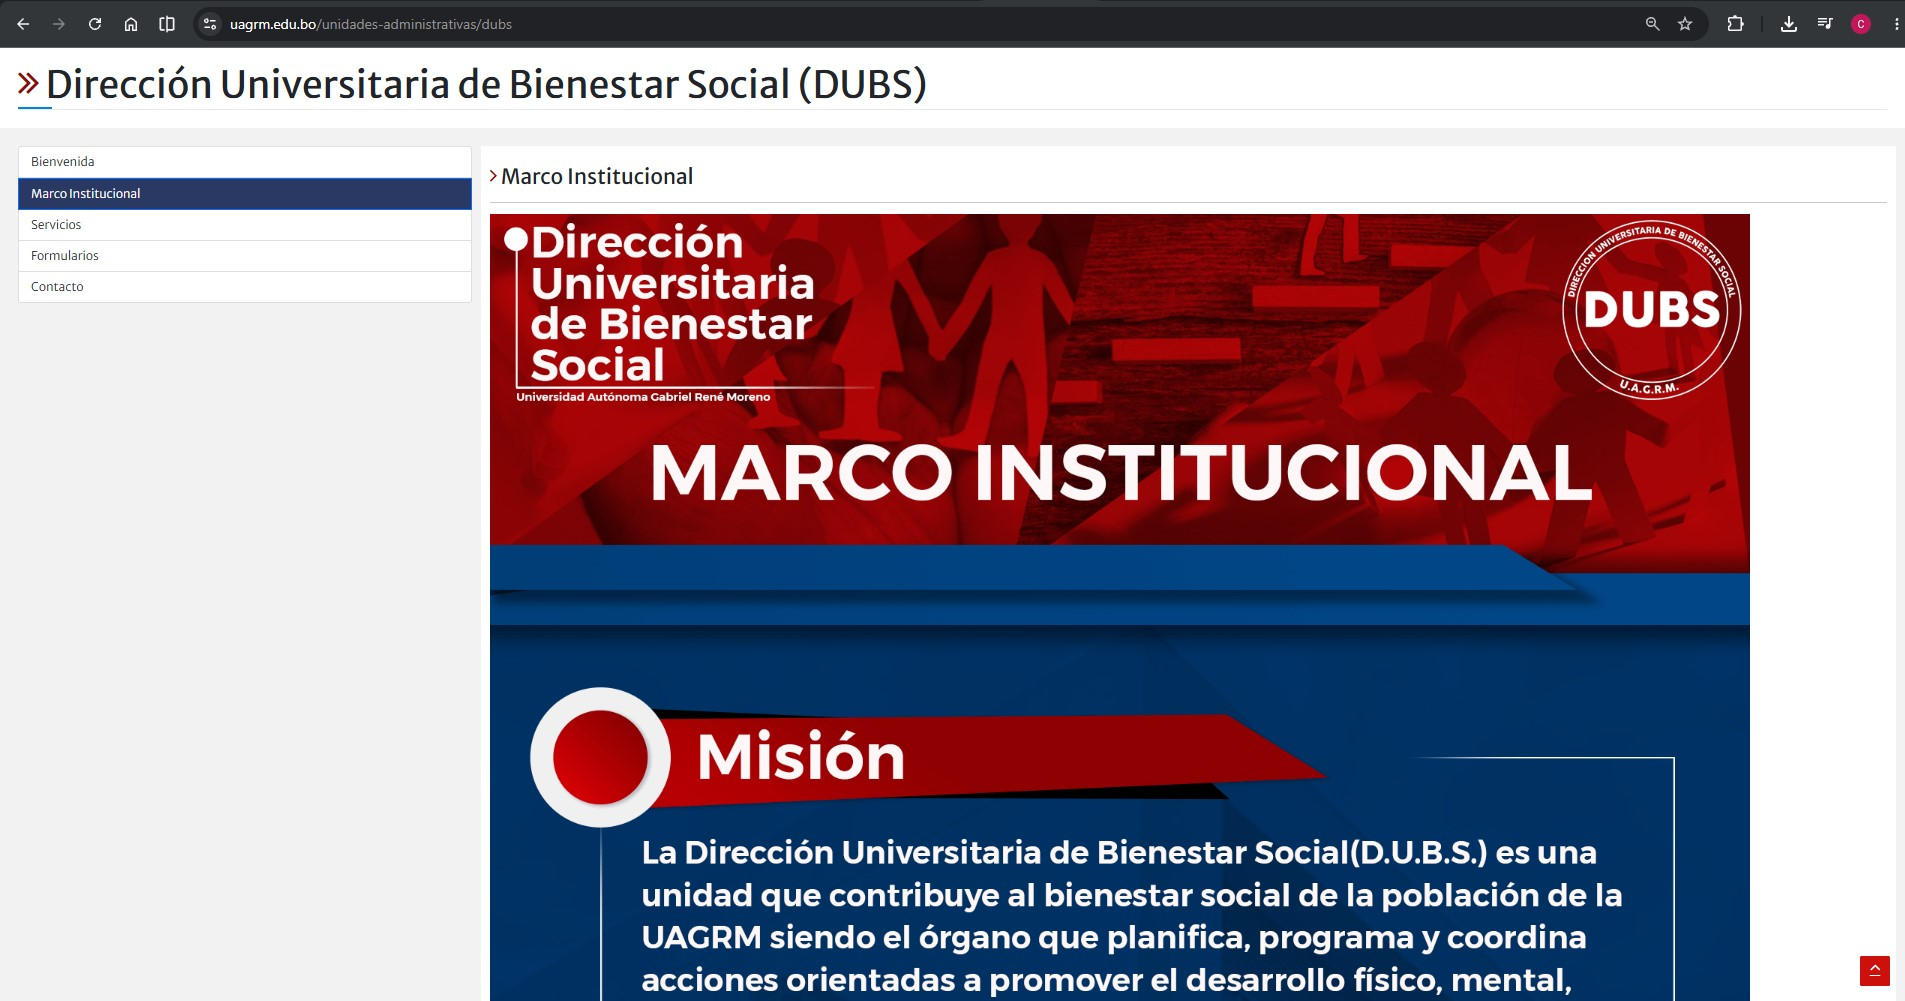
\includegraphics[width=0.85\linewidth]{images/010_PaginaWeb_DUBSS.jpg}

\smallskip
\noindent\raggedright\textit{Nota.} Captura de pantalla del sitio web institucional. Recuperado el 13 de septiembre de 2026, de \url{https://dubs.uagrm.edu.bo/}
\end{figure}

\textbf{Facebook:} \url{https://www.facebook.com/DireccionUniversitariaDeBienestarSocial}

\begin{figure}[H]
\caption{Página oficial de Facebook de la Dirección Universitaria de Bienestar Social y Salud (DUBSS)}
\label{fig:facebook_dubss}
\centering

\includegraphics[width=0.4\linewidth]{images/011_Facebook_DUBSS.jpg}

\smallskip
\noindent\raggedright\textit{Nota.} Captura de pantalla de la red social Facebook. Recuperado el 13 de septiembre de 2026, de \url{https://www.facebook.com/DireccionUniversitariaDeBienestarSocial}
\end{figure}

\textbf{Instagram:} \url{https://www.instagram.com/dubs_uagrm/}

\begin{figure}[H]
\caption{Perfil oficial de Instagram de la Dirección Universitaria de Bienestar Social y Salud (DUBSS)}
\label{fig:instagram_dubss}
\centering

\includegraphics[width=0.4\linewidth]{images/012_Instagram_DUBSS.jpg}

\smallskip
\noindent\raggedright\textit{Nota.} Captura de pantalla de la red social Instagram. Recuperado el 13 de septiembre de 2026, de \url{https://www.instagram.com/dubs_uagrm/}
\end{figure}


\textbf{Correo Electrónico:} dubs@uagrm.edu.bo

\textbf{Teléfono / WhatsApp de Atención:} +591 61537017


% ------------------------------------------------------------------------------
% 3.2. ESTRUCTURA ORGANIZACIONAL
% ------------------------------------------------------------------------------
\dbsa{\wn{3.2}. Estructura Organizacional}\label{sec:estructura_organizacional}
% [INSTRUCCIÓN]: Organigrama, roles, áreas funcionales y responsabilidades del equipo de trabajo.

\begin{figure}[H]
\caption{Organigrama de la Dirección Universitaria de Bienestar Social y Salud (DUBSS)}
\label{fig:organigrama_dubss}
\centering
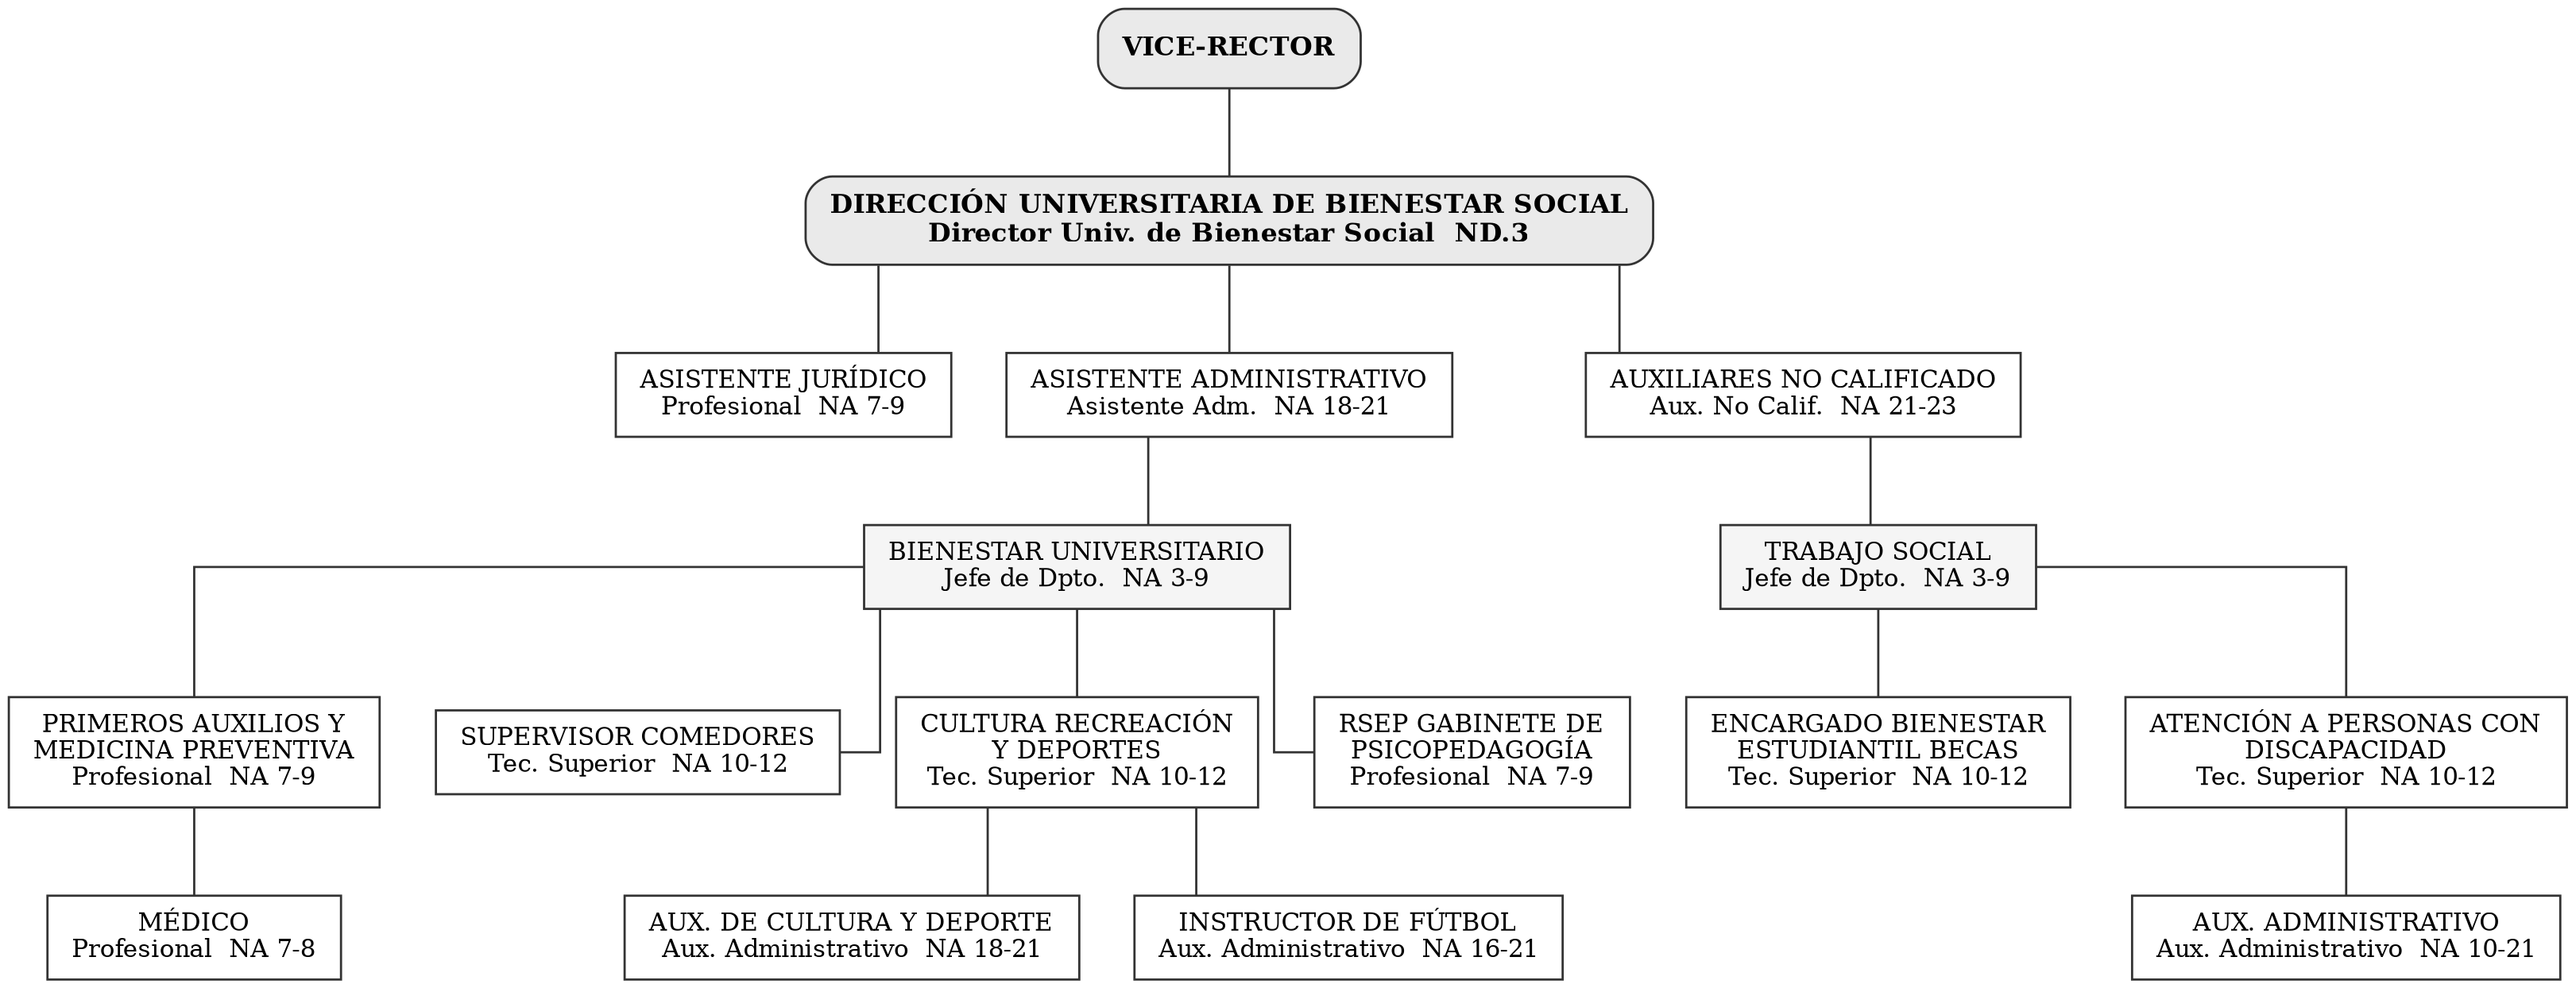
\includegraphics[width=\textwidth]{images/005_Organigrama_DUBSS.png}

\smallskip
\noindent\raggedright\textit{Nota.} Elaboración propia en base a los datos institucionales de la DUBSS.
\end{figure}

\clearpage
% ------------------------------------------------------------------------------
% 3.3. UBICACIÓN E INFRAESTRUCTURA
% ------------------------------------------------------------------------------
\dbsa{\wn{3.3}. Ubicación e Infraestructura}\label{sec:ubicacion_infraestructura}
% [INSTRUCCIÓN]: Ubicación geográfica de la sede operativa, centros de datos y facilidades técnicas.

\begin{figure}[H]
\caption{Comedor Universitario de la Universidad Autónoma Gabriel René Moreno}
\label{fig:comedor_universitario}
\centering
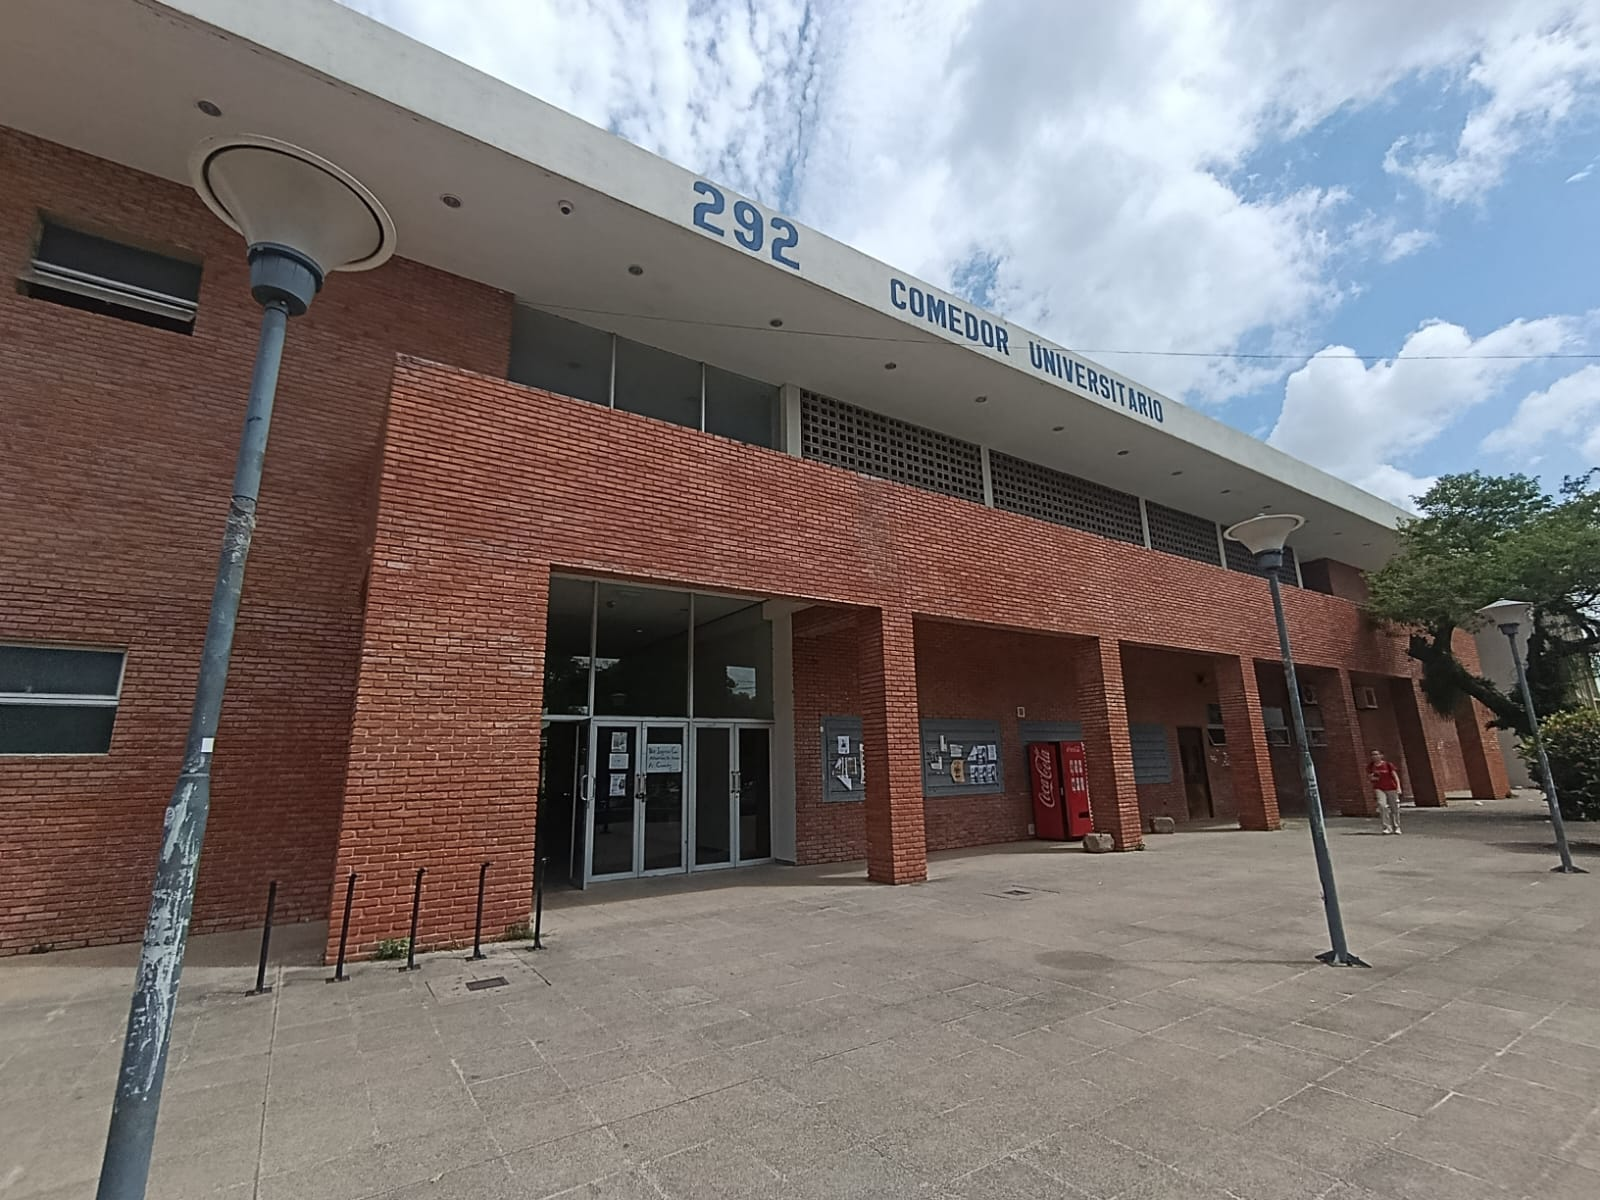
\includegraphics[width=0.5\textwidth]{images/006_Comedor_Universitario.jpeg}

\smallskip
\noindent\raggedright\textit{Nota.} Elaboración propia.
\end{figure}

\begin{figure}[H]
\caption{Oficinas de la Dirección Universitaria de Bienestar Social y Salud (DUBSS)}
\label{fig:oficinas_dubss}
\centering
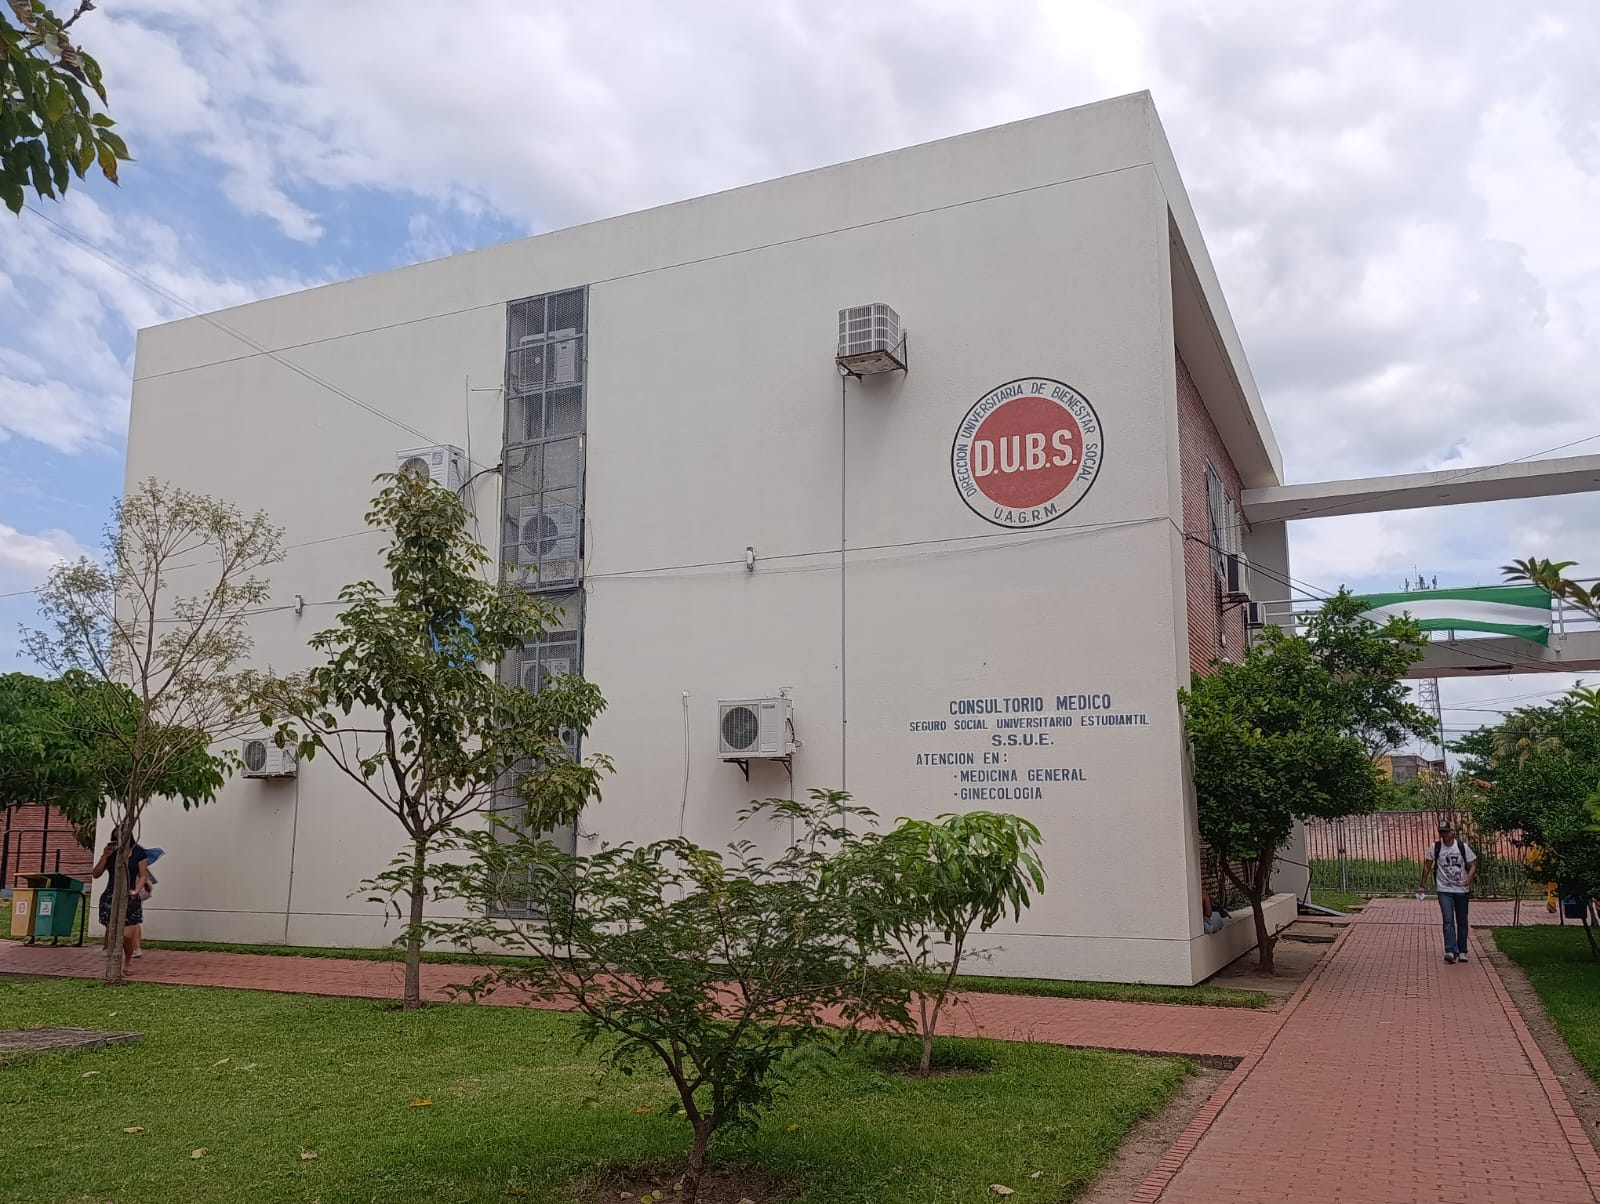
\includegraphics[width=0.5\textwidth]{images/007_Oficinas_DUBSS.jpeg}

\smallskip
\noindent\raggedright\textit{Nota.} Elaboración propia.
\end{figure}

\clearpage
\begin{figure}[H]
\caption{Ubicación de las instalaciones de la DUBSS en el campus universitario}
\label{fig:ubicacion_dubss}
\centering
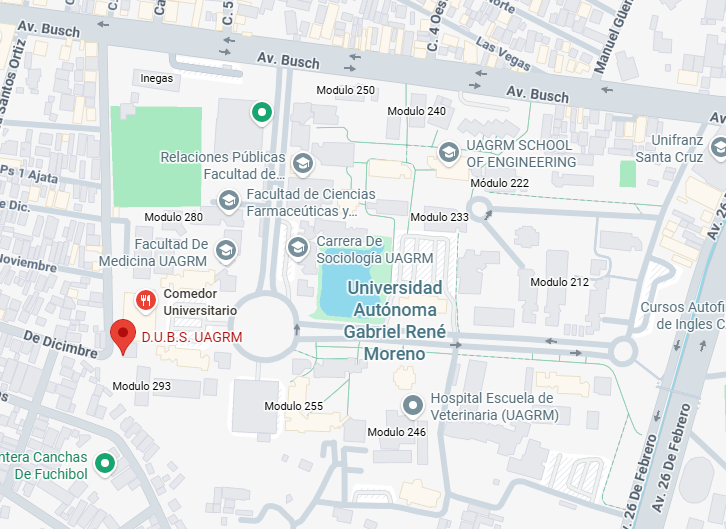
\includegraphics[width=\textwidth]{images/008_Ubicacion_DUBSS.png}

\smallskip
\noindent\raggedright\textit{Nota.} Elaboración propia a partir de una captura de Google Maps.
\end{figure}

% ------------------------------------------------------------------------------
% 3.4. MODELO DE NEGOCIO
% ------------------------------------------------------------------------------
\dbsa{\wn{3.4}. Modelo de Negocio}\label{sec:modelo_negocio}
% [INSTRUCCIÓN]: Propuesta de valor, segmentos de clientes, fuentes de ingresos y esquema de sostenibilidad (lienzo Canvas si aplica).

\begin{figure}[H]
\caption{Modelo de negocio propuesto para el Sistema de Información de la Beca Comedor}
\label{fig:modelo_negocio}
\centering
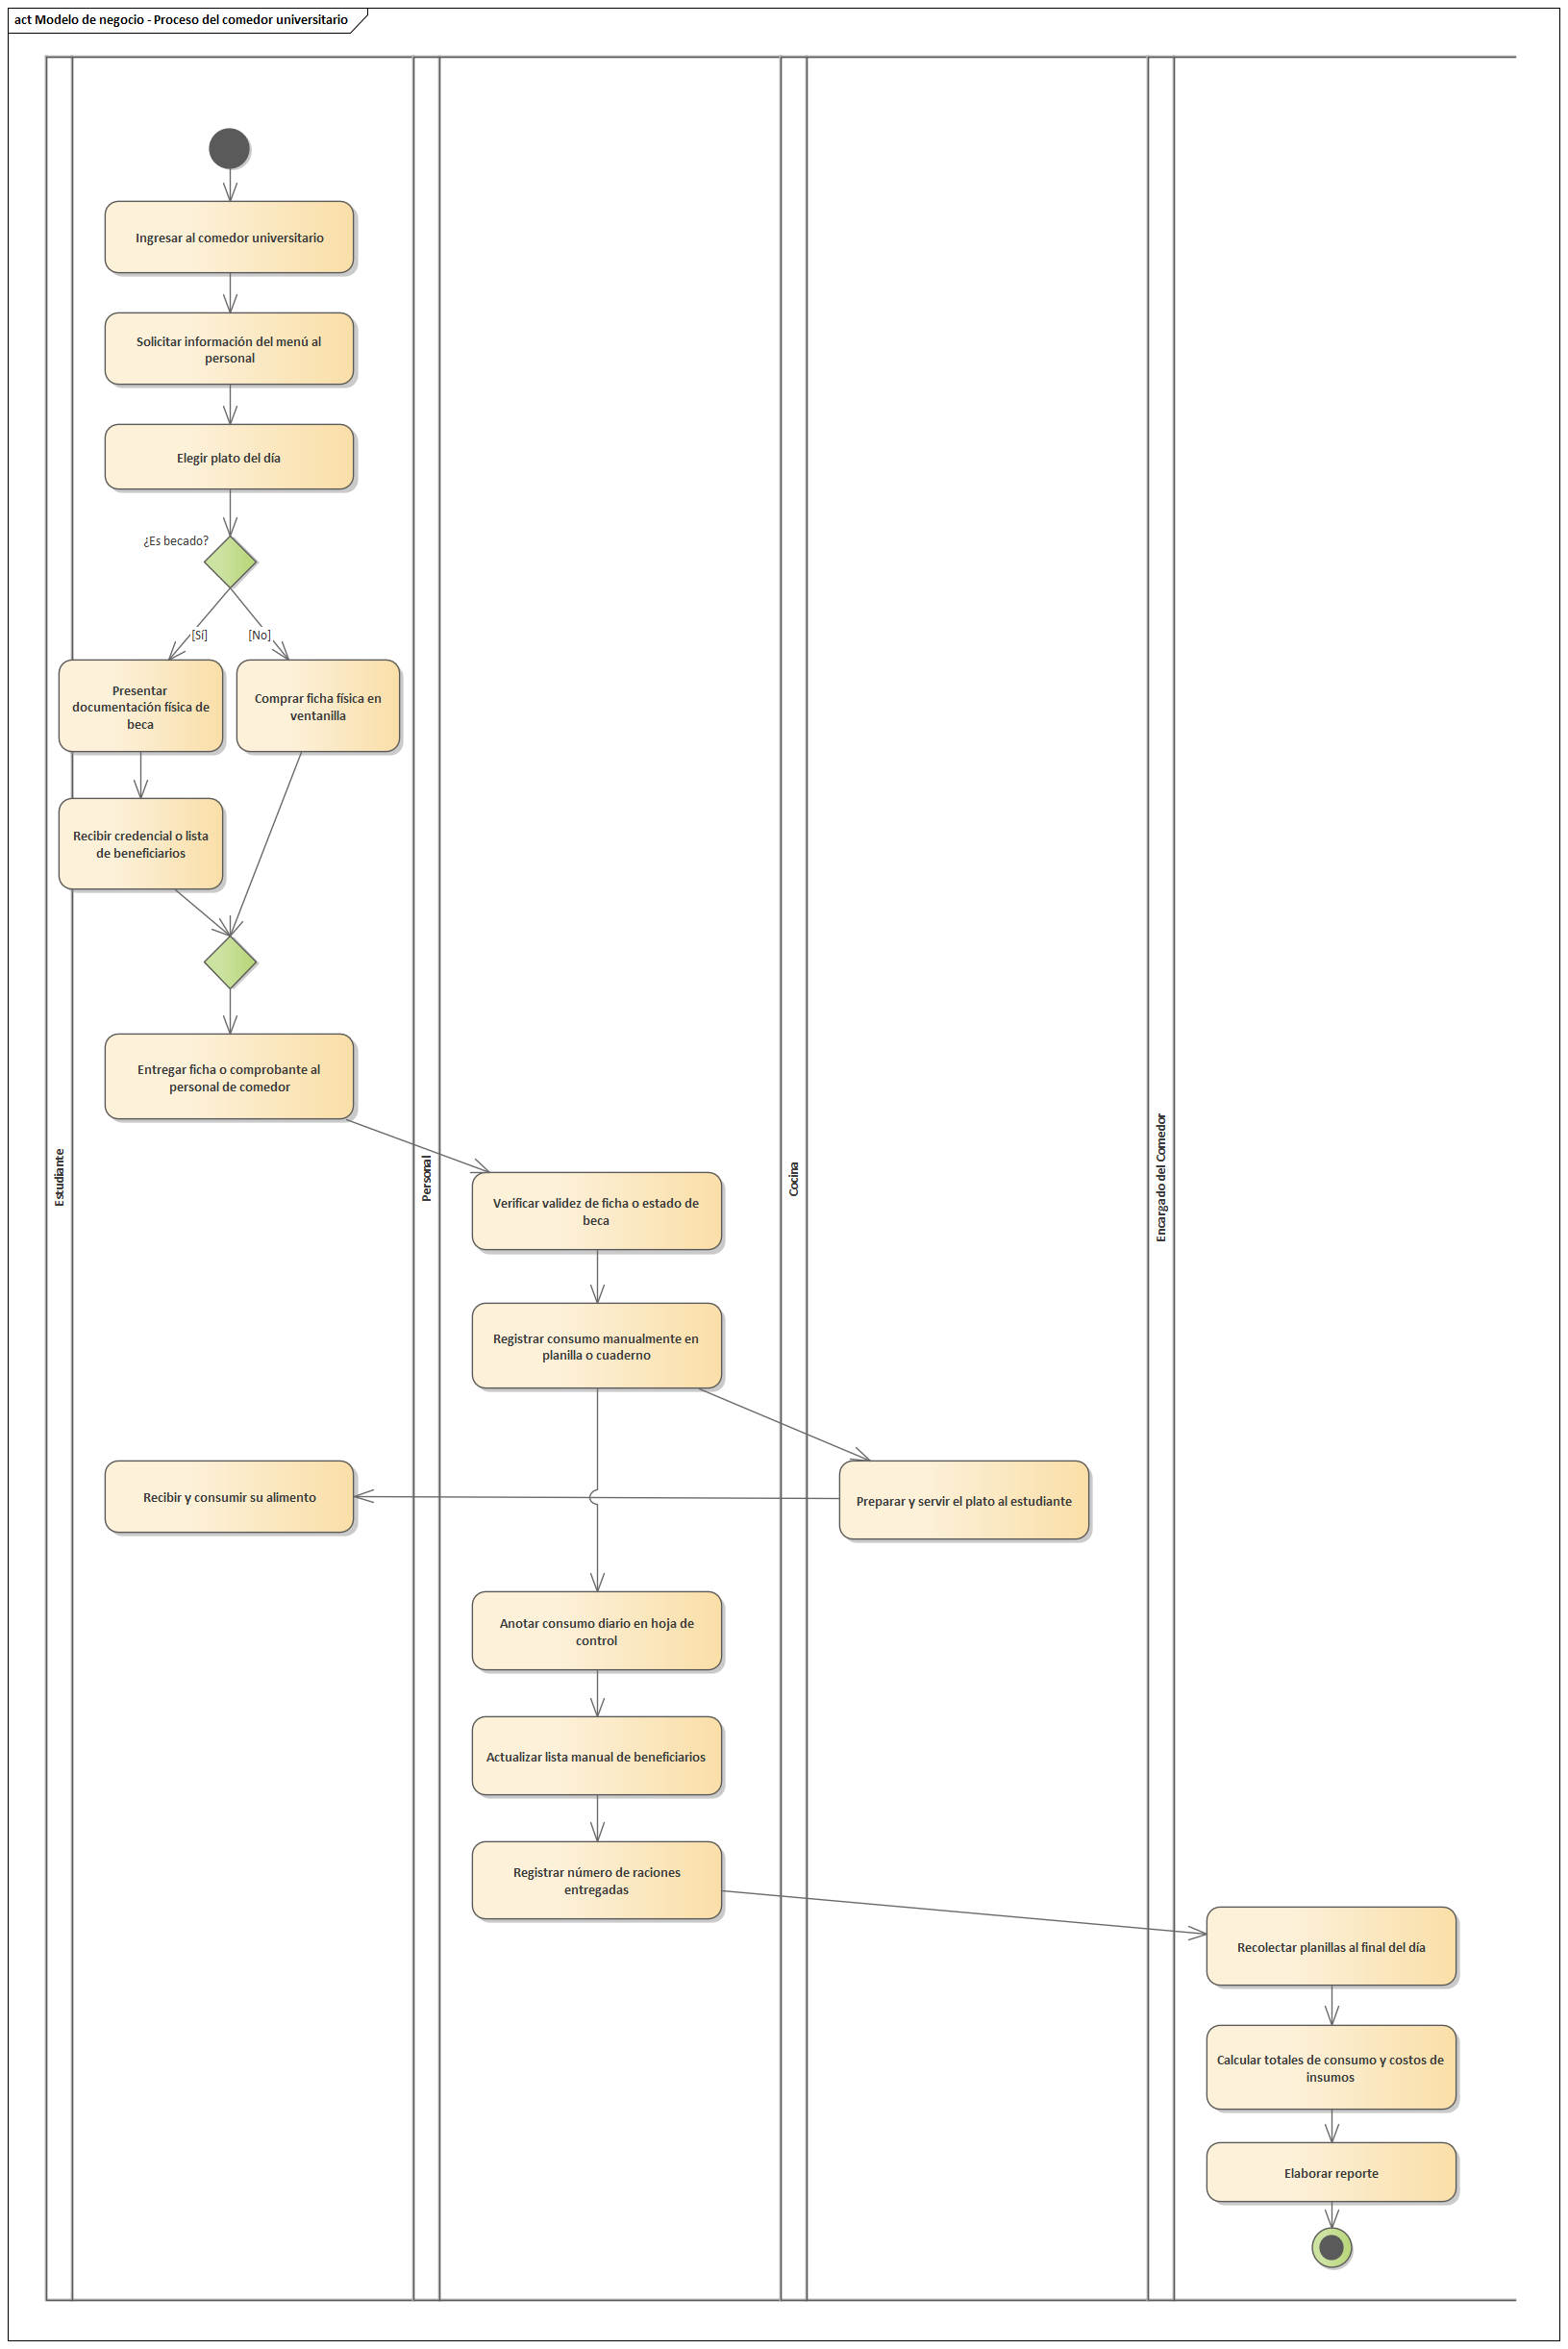
\includegraphics[width=\textwidth,height=0.78\textheight,keepaspectratio]{images/009_Modelo_Negocio.png}

\smallskip
\noindent\raggedright\textit{Nota.} Elaboración propia con información de la DUBSS.
\end{figure}

% ------------------------------------------------------------------------------
% 3.5. FLUJO OPERATIVO
% ------------------------------------------------------------------------------
\dbsa{\wn{3.5}. Flujo Operativo}\label{sec:flujo_operativo}

El flujo operativo describe cómo se desarrolla actualmente, en la Dirección Universitaria de Bienestar Social y Salud (DUBSS), el proceso de postulación y adjudicación de la Beca Comedor. En él intervienen el postulante, que presenta su carpeta con la documentación de respaldo; el personal de Trabajo Social, que revisa los documentos y califica la solicitud; y la Encargada de Sistemas, que incorpora el rendimiento académico y calcula el puntaje total que determina la adjudicación. La Figura~\ref{fig:postulacion_beca} representa las actividades de este proceso y las responsabilidades de cada actor.

\begin{figure}[H]
\caption{Diagrama de actividades del proceso de postulación a la Beca Comedor}
\label{fig:postulacion_beca}
\centering
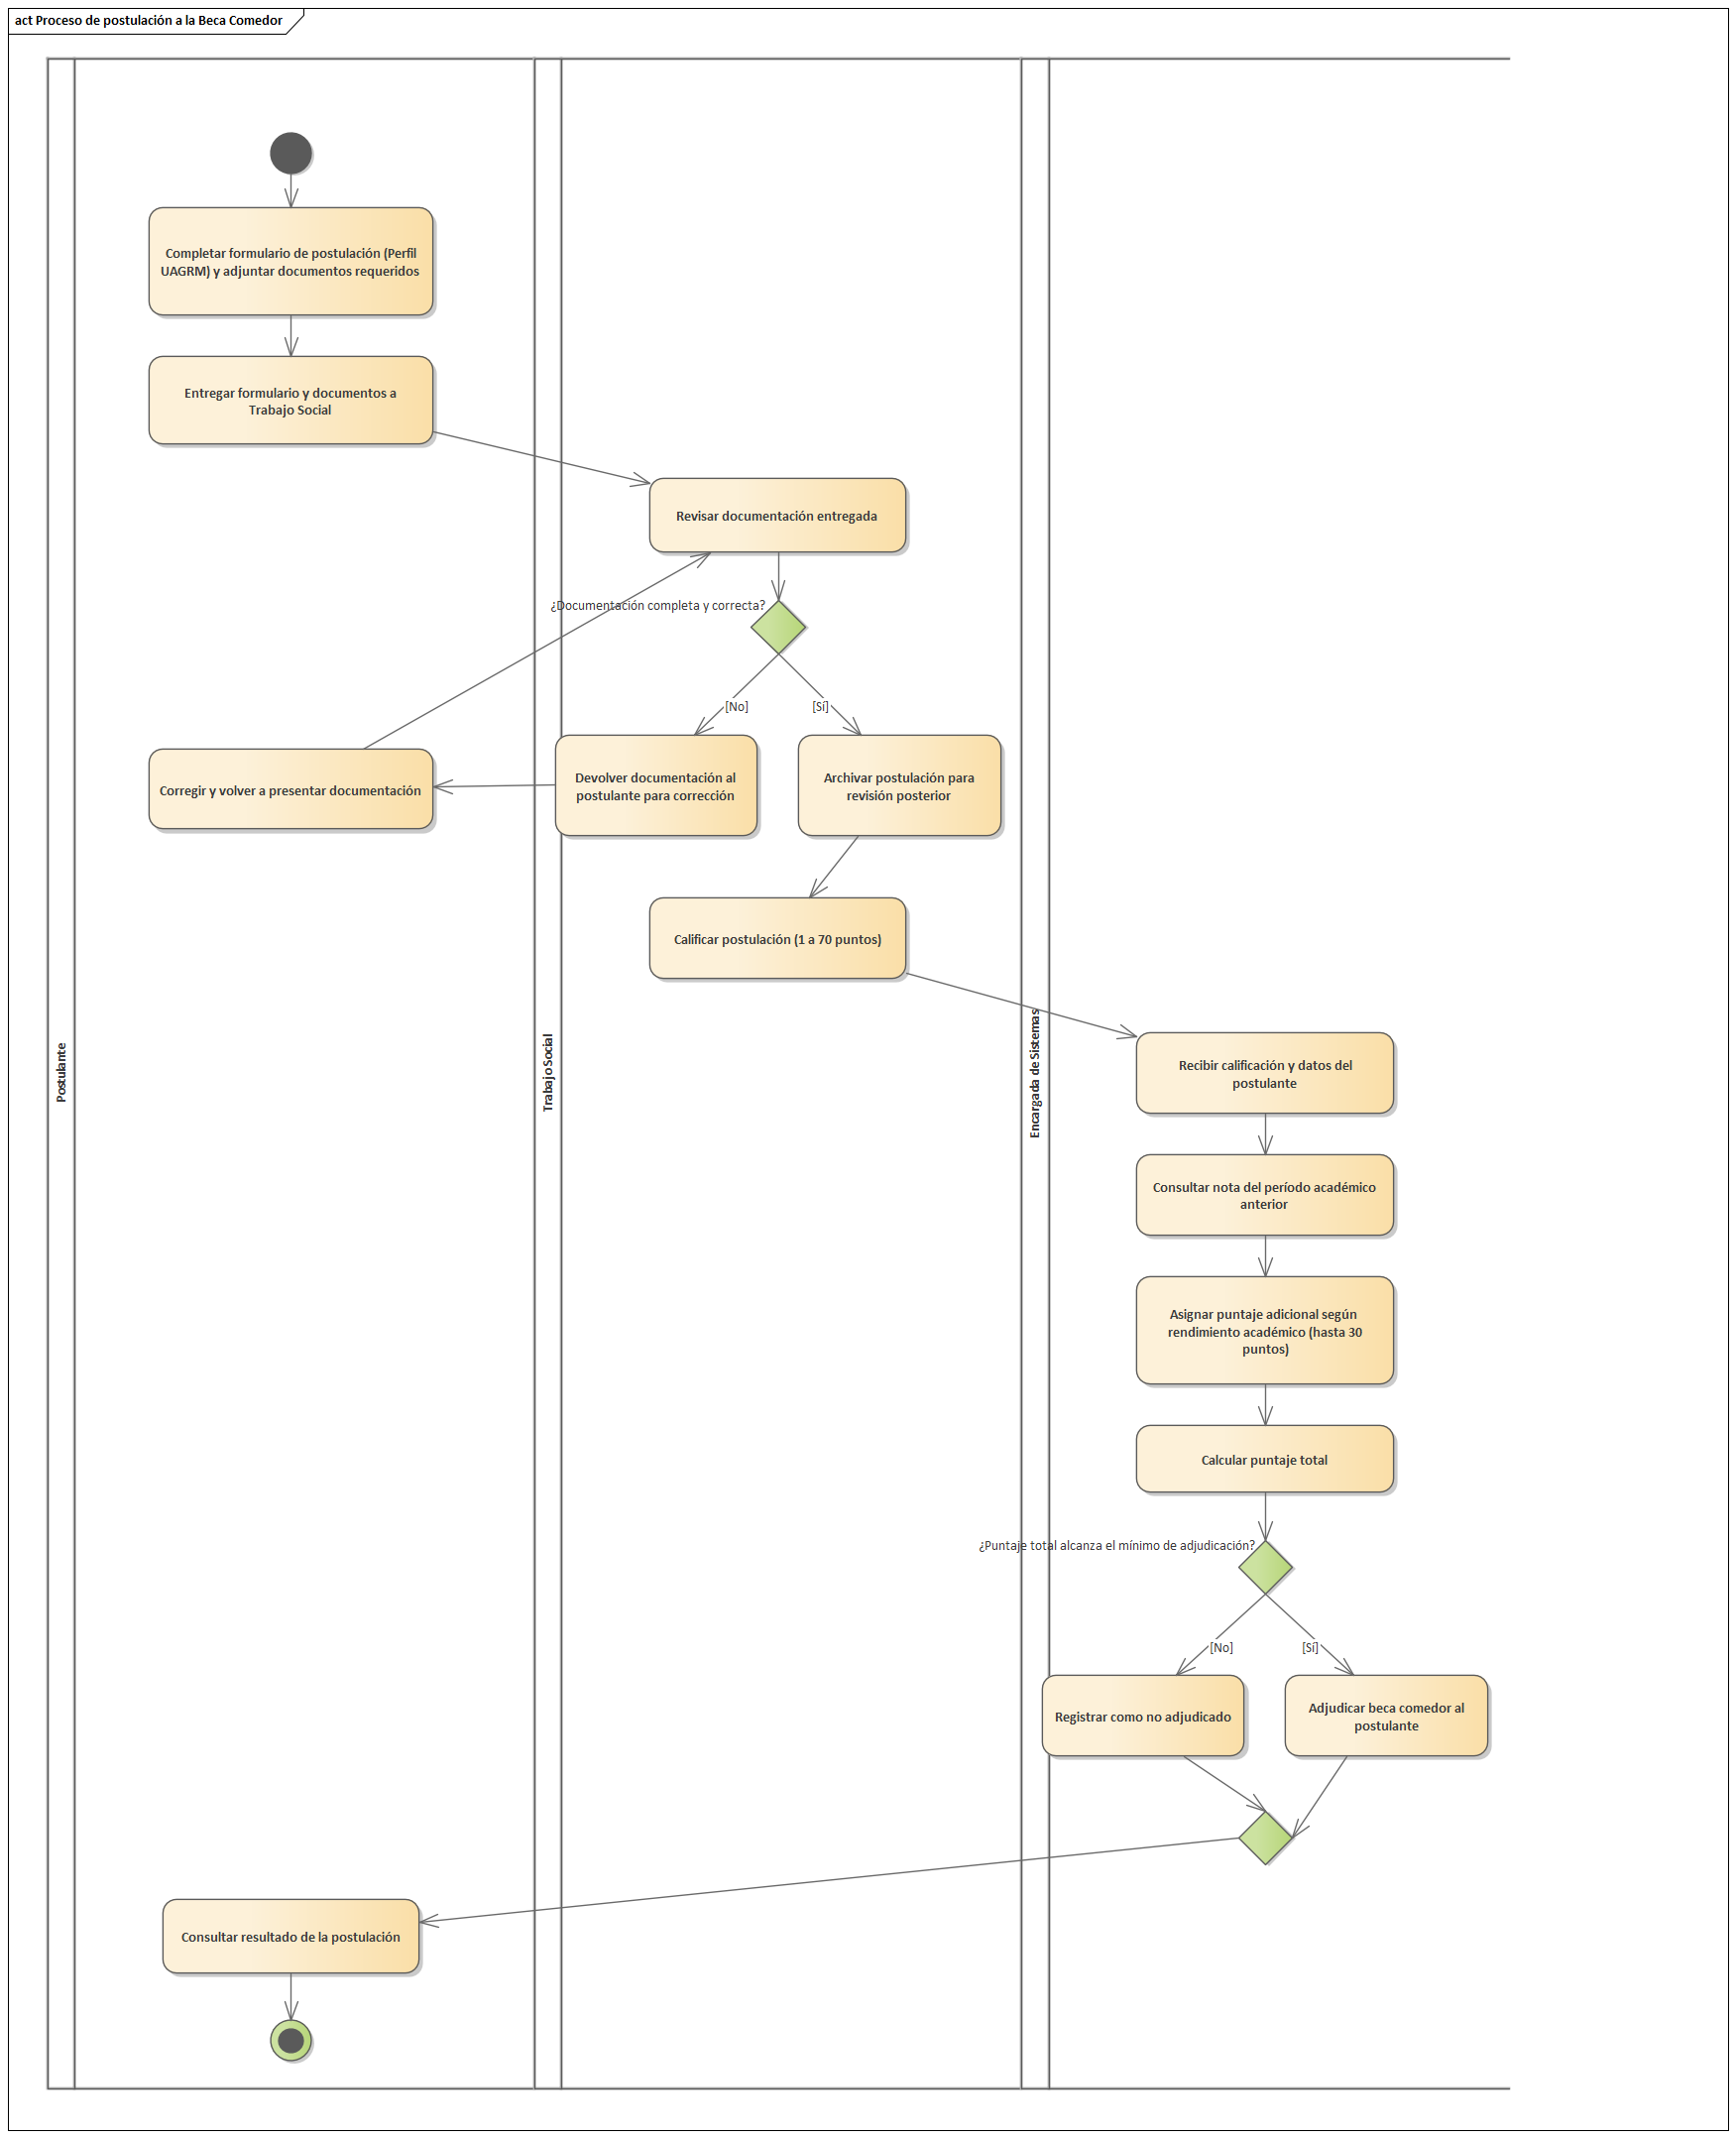
\includegraphics[width=\textwidth,height=0.8\textheight,keepaspectratio]{images/017_Postulacion_Beca.png}

\smallskip
\noindent\raggedright\textit{Nota.} Elaboración propia basado en la entrevista con el personal de la DUBSS.
\end{figure}


\paragraph{3.1.7.2. Datos.}

% [PENDIENTE]: Redactar "Datos".

\paragraph{3.1.7.3. Arquitectura.}

\subparagraph{3.1.7.3.1. Diagrama de despliegue.}

% [PENDIENTE]: Redactar "Diagrama de despliegue".

\subsubsection{3.1.8. Definición de criterios de calidad}

% [PENDIENTE]: Redactar "Definición de criterios de calidad".

\subsubsection{3.1.9. Lista priorizada de casos de uso}

La identificación, priorización y detalle de los casos de uso se desarrolla en las secciones 3.2.5 a 3.2.8.



% ==============================================================================
% 3.2 CAPTURA DE REQUISITOS (flujo de trabajo PUDS)
% Reutiliza el ERS (IEEE 830, cap. 4 de main.tex) y la captura de requisitos (cap. 5 de main.tex).
% ==============================================================================
\subsection{3.2. Captura de Requisitos}\label{sec:v2_captura_requisitos}

Este flujo de trabajo del PUDS identifica los requisitos del sistema. Las secciones 3.2.1 a 3.2.3 formalizan los requisitos según el estándar IEEE 830 (Especificación de Requisitos de Software) y las secciones 3.2.4 a 3.2.8 identifican los actores y los casos de uso, los priorizan, detallan cada uno y los integran en el diagrama general de casos de uso.

% ------------------------------------------------------------------------------
% 4.1. INTRODUCCIÓN
% ------------------------------------------------------------------------------
\wfa{\wn{4.1}. Introducción}\label{sec:ieee_introduccion}

\wfb{\wn{4.1}.1. Propósito}\label{sec:ieee_proposito}
% [INSTRUCCIÓN]: Definir el propósito específico del documento ERS y su audiencia objetivo.

El presente documento tiene como propósito definir, de manera clara, completa y sin ambigüedades, las funcionalidades y restricciones requeridas para el desarrollo del Sistema de Información Web y Móvil para la Postulación y Preselección Automatizada de la Beca Comedor mediante Inteligencia Artificial, con Reportes de Business Intelligence para la Dirección Universitaria de Bienestar Social y Salud (DUBSS) de la Universidad Autónoma Gabriel René Moreno. Esta Especificación de Requisitos del Software (ERS) está dirigida al equipo de desarrollo encargado de la construcción del sistema, al personal directivo y administrativo de la Dirección Universitaria de Bienestar Social y Salud (DUBSS) y a los docentes evaluadores del proyecto de grado, con el objetivo de establecer un acuerdo formal sobre el alcance, el comportamiento esperado y las restricciones del software antes de iniciar las etapas de diseño e implementación.

\wfb{\wn{4.1}.2. Ámbito del Sistema}\label{sec:ieee_ambito}
% [INSTRUCCIÓN]: Nombre del producto software, alcance operativo, beneficios y metas generales.

\textbf{Nombre del proyecto:} Sistema de Información Web y Móvil para la Postulación y Preselección Automatizada de la Beca Comedor mediante Inteligencia Artificial, con Reportes de Business Intelligence para la Dirección Universitaria de Bienestar Social y Salud (DUBSS) de la Universidad Autónoma Gabriel René Moreno.

El sistema comprenderá las siguientes funcionalidades principales:

\begin{itemize}
    \item Registro y autenticación de postulantes a través de las plataformas web y móvil.
    \item Postulación en línea a la Beca Comedor mediante el llenado de formularios socioeconómicos digitales.
    \item Preselección automatizada de solicitudes empleando un modelo de Inteligencia Artificial y Machine Learning que precalifica algorítmicamente el nivel de vulnerabilidad socioeconómica de cada postulante.
    \item Gestión administrativa de los expedientes finalistas, incluyendo la auditoría física de respaldos y el registro de los estudiantes efectivamente becados.
    \item Registro y control de la asistencia física y digital de los becarios al Comedor Universitario.
    \item Generación de reportes y dashboards de Business Intelligence con proyecciones predictivas que apoyen la toma de decisiones institucionales.
\end{itemize}

Entre los principales beneficios que otorgará el sistema a la DUBSS se encuentran la reducción drástica del tiempo y del personal destinado a la revisión manual de carpetas, la eliminación del cuello de botella administrativo generado por las 20,000 solicitudes recibidas por gestión, la incorporación de un criterio de selección objetivo, transparente y auditable, y la disposición de información oportuna y confiable para la planificación y rendición de cuentas institucional.

\wfb{\wn{4.1}.3. Definiciones, Acrónimos y Abreviaturas}\label{sec:ieee_definiciones}
% [INSTRUCCIÓN]: Glosario de términos técnicos, siglas y acrónimos necesarios para interpretar el documento.

La Tabla~\ref{tab:definiciones_abreviaturas} resume los principales términos, siglas y acrónimos empleados a lo largo del presente documento.

\begin{table}[H]
\caption{Definiciones, acrónimos y abreviaturas empleados en el documento}
\label{tab:definiciones_abreviaturas}
\begin{threeparttable}
\begin{tabular}{>{\raggedright\arraybackslash}p{3cm} >{\raggedright\arraybackslash}p{10cm}}
\toprule
Nombre & Descripción \\
\midrule
DUBSS & Dirección Universitaria de Bienestar Social y Salud, unidad de la UAGRM responsable de la Beca Comedor. \\
Administrador & Personal de la DUBSS que audita, valida y gestiona las postulaciones dentro del sistema. \\
Postulante & Estudiante de la UAGRM que solicita el beneficio de la Beca Comedor a través del sistema. \\
Usuario & Persona que interactúa con el software, ya sea en calidad de postulante o de administrador. \\
RF & Requerimiento funcional. \\
RNF & Requerimiento no funcional. \\
ERS & Especificación de Requisitos del Software. \\
PCN & Prueba de caja negra. \\
IA & Inteligencia Artificial. \\
ML & Machine Learning (aprendizaje automático). \\
PLN & Procesamiento de Lenguaje Natural. \\
API & Interfaz de Programación de Aplicaciones. \\
UI/UX & Interfaz de Usuario y Experiencia de Usuario. \\
JS & Lenguaje de programación JavaScript. \\
\bottomrule
\end{tabular}
\begin{tablenotes}
\item \textit{Nota.} Elaboración propia.
\end{tablenotes}
\end{threeparttable}
\end{table}

\wfb{\wn{4.1}.4. Referencias}\label{sec:ieee_referencias}
% [INSTRUCCIÓN]: Lista de documentos de referencia, normativas institucionales y estándares técnicos.

Los principales estándares, libros y artículos empleados para las definiciones y el desarrollo de este capítulo son los siguientes:

\begin{itemize}
    \item \textcite{ieee830_1998} y \textcite{iso29148_2011}.
    \item \textcite{pressman2010ingenieria}.
    \item \textcite{sommerville2011ingenieria}.
\end{itemize}

\wfb{\wn{4.1}.5. Visión General del Documento}\label{sec:ieee_vision_general}
% [INSTRUCCIÓN]: Breve descripción de la organización del resto de la especificación de requisitos.

El presente documento se compone de tres secciones (Introducción, Descripción General y Requisitos Específicos) que describen detalladamente el producto a desarrollarse. En primer lugar, la sección de Introducción establece el propósito, el ámbito, las definiciones y la visión general del documento. A continuación, la sección de Descripción General sitúa al sistema dentro de su contexto de uso, describiendo sus funciones principales, las características de sus usuarios y las restricciones y suposiciones bajo las cuales operará. Finalmente, la sección de Requisitos Específicos detalla de manera formal cada uno de los requisitos funcionales, no funcionales y de interfaz de usuario que deberá satisfacer el sistema.

% ------------------------------------------------------------------------------
% 4.2. DESCRIPCIÓN GENERAL
% ------------------------------------------------------------------------------
\subsection{4.2. Descripción General}\label{sec:ieee_descripcion_general}

\subsubsection{4.2.1. Perspectiva del Producto}\label{sec:ieee_perspectiva}
% [INSTRUCCIÓN]: Contexto del producto: sistema autónomo o módulo integrado en un entorno universitario mayor.

El Sistema de Información Web y Móvil para la Postulación y Preselección Automatizada de la Beca Comedor es un producto de software independiente y de nuevo desarrollo; no constituye un módulo dentro de una plataforma empresarial mayor ni reemplaza algún sistema institucional preexistente, dado que la DUBSS gestiona actualmente este proceso de forma manual. No obstante, el sistema sí se relaciona con dos actores externos a su núcleo funcional: por un lado, el punto de control de asistencia del Comedor Universitario, donde los postulantes seleccionados validan físicamente su condición de becados; y por otro, el personal directivo de la DUBSS, que consume los reportes y proyecciones de Business Intelligence generados por el sistema para la toma de decisiones institucionales.

\subsubsection{4.2.2. Funciones del Producto}\label{sec:ieee_funciones}
% [INSTRUCCIÓN]: Resumen ejecutivo de las capacidades y operaciones principales del software.

De manera general, el sistema permitirá a los postulantes registrarse y enviar su postulación a la Beca Comedor completando un formulario socioeconómico digital desde la web o la aplicación móvil. Asimismo, el sistema precalificará automáticamente cada solicitud mediante un modelo de inteligencia artificial que estima el nivel de vulnerabilidad socioeconómica del postulante, y notificará a los finalistas para que presenten su documentación física de respaldo. Por su parte, el personal de la DUBSS podrá auditar y validar dichos expedientes, administrar el registro de los estudiantes efectivamente becados y controlar su asistencia al Comedor Universitario. Finalmente, el sistema generará reportes y dashboards de Business Intelligence que resuman el comportamiento histórico de las postulaciones y proyecten tendencias futuras para apoyar la planificación institucional. La Figura~\ref{fig:diagrama_cu} representa gráficamente los actores del sistema y los casos de uso principales asociados a cada uno.

\begin{figure}[H]
\caption{Diagrama de casos de uso del Sistema Web y Móvil de Postulación y Preselección de la Beca Comedor}
\label{fig:diagrama_cu}
\centering
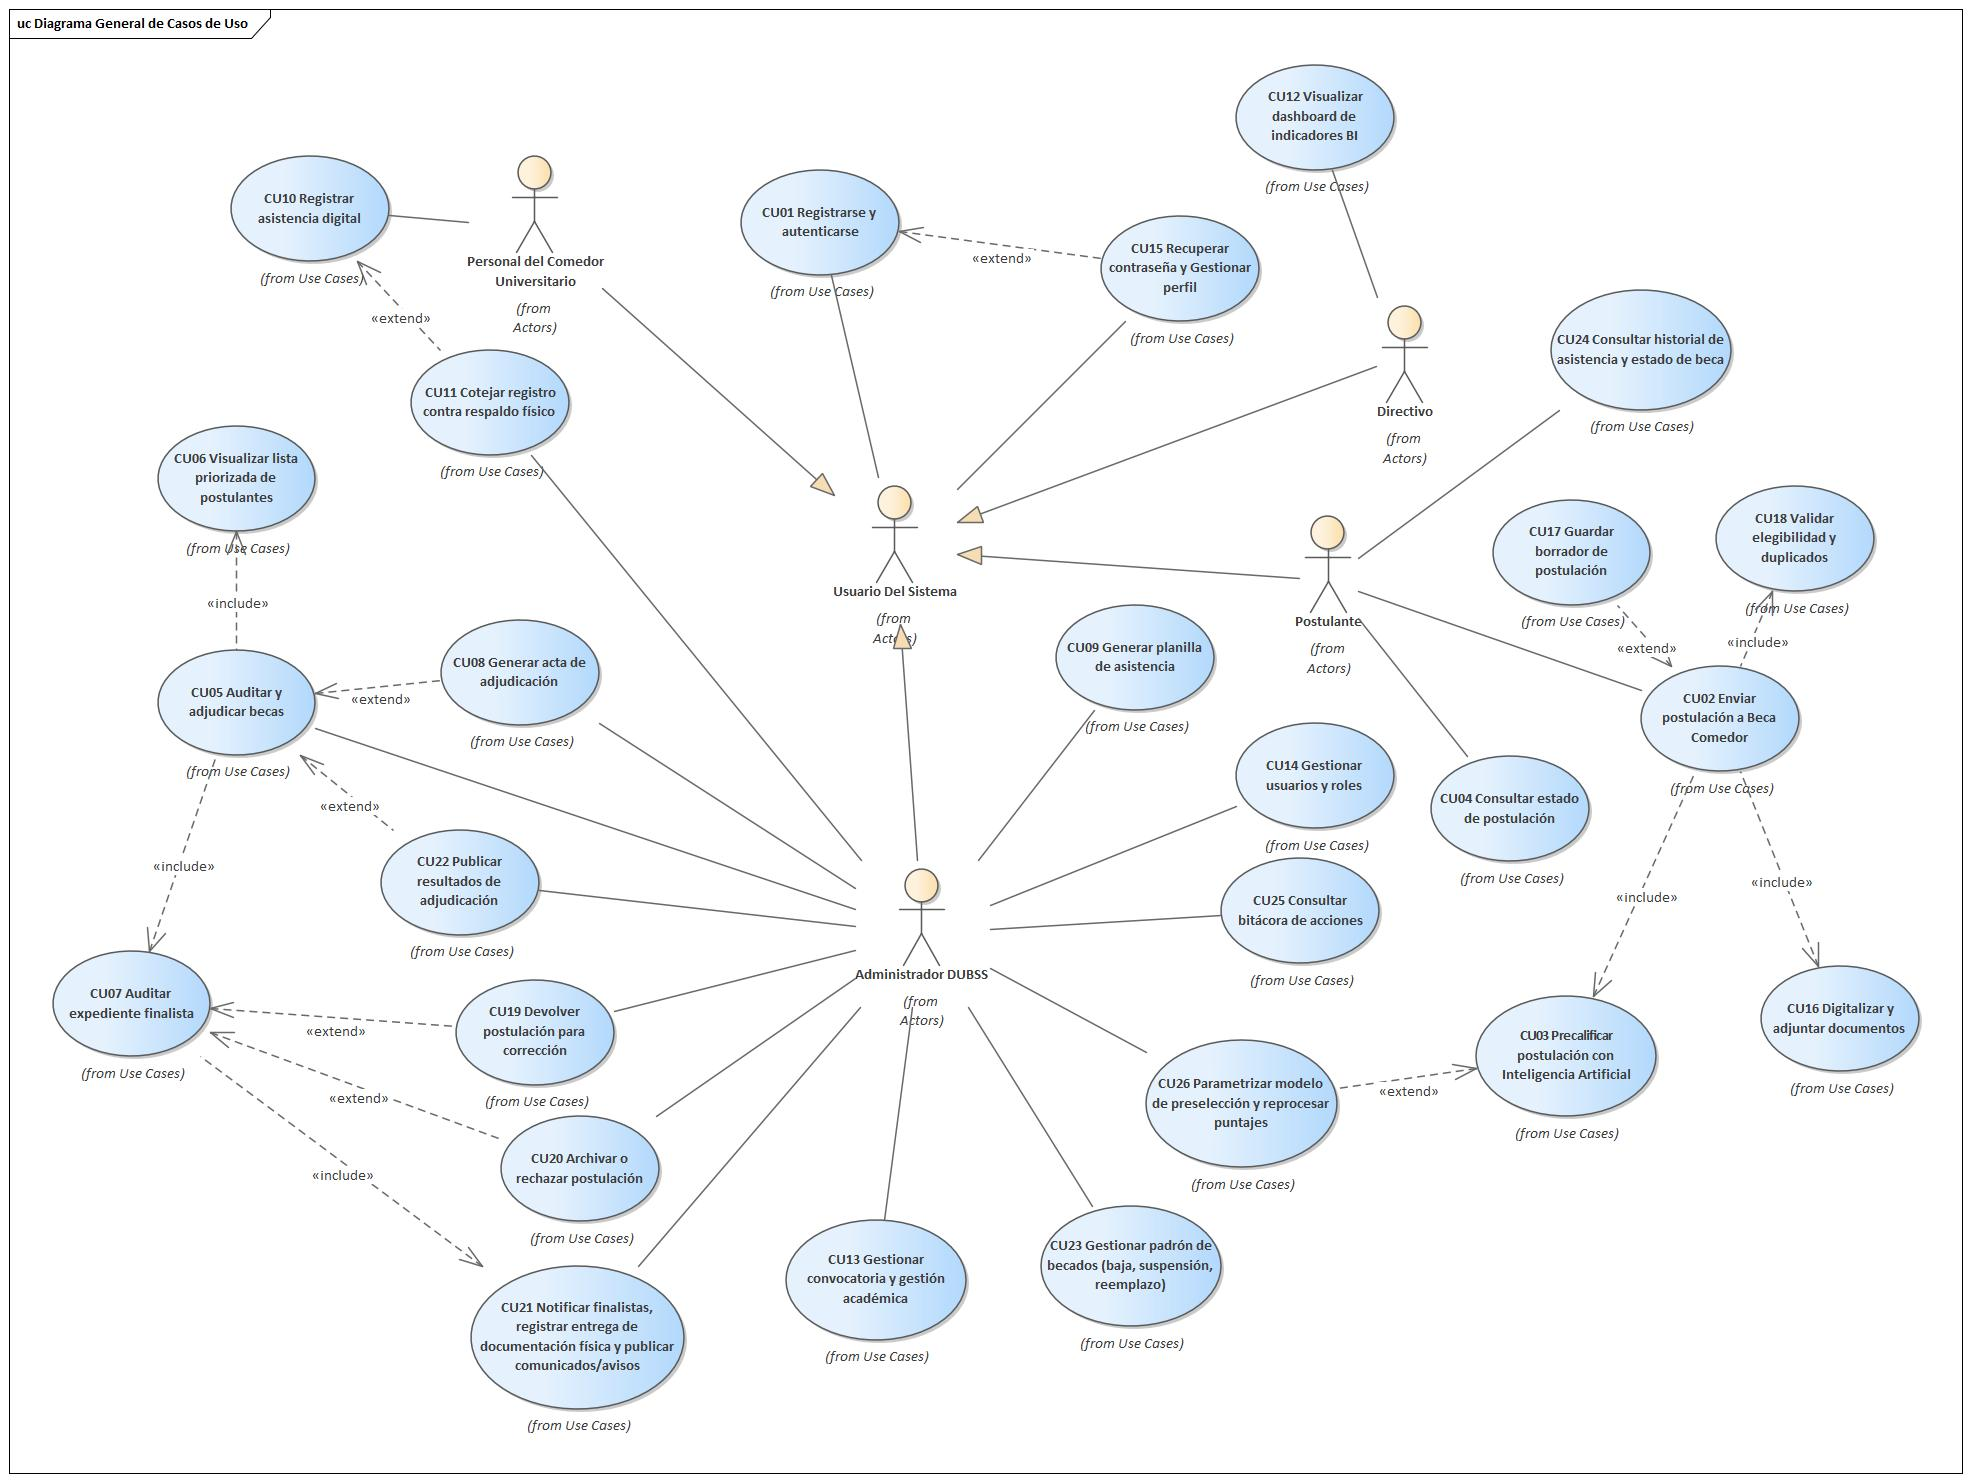
\includegraphics[width=\textwidth,height=0.85\textheight,keepaspectratio]{images/019_Diagrama_General_CU.jpg}

\smallskip
\noindent\raggedright\textit{Nota.} Elaboración propia.
\end{figure}

\subsubsection{4.2.3. Características de los Usuarios}\label{sec:ieee_caracteristicas_usuarios}
% [INSTRUCCIÓN]: Perfiles de usuario (estudiantes postulantes, administradores, personal de comedor, etc.).

La Tabla~\ref{tab:caracteristicas_usuarios} describe los tipos de usuario del sistema, sus responsabilidades y el nivel de conocimiento técnico requerido para su uso.

\begin{table}[H]
\caption{Tipos de usuario del sistema y sus características}
\label{tab:caracteristicas_usuarios}
\begin{threeparttable}
\begin{tabular}{>{\raggedright\arraybackslash}p{3cm} >{\raggedright\arraybackslash}p{6.5cm} >{\raggedright\arraybackslash}p{3.5cm}}
\toprule
Tipo de usuario & Descripción & Conocimiento técnico requerido \\
\midrule
Postulante & Estudiante de la UAGRM que se registra y postula a la Beca Comedor a través de la web o la aplicación móvil. & Básico: manejo elemental de aplicaciones web y móviles. \\
Administrador DUBSS & Personal administrativo que audita la documentación física de los finalistas y gestiona el proceso de selección dentro del sistema. & Básico: manejo de ofimática y de un panel web administrativo. \\
Directivo DUBSS (Gerente) & Personal directivo que visualiza el dashboard de reportes gráficos y proyecciones de Business Intelligence para la toma de decisiones. & Básico: interpretación de reportes y gráficos, sin necesidad de conocimientos de programación. \\
\bottomrule
\end{tabular}
\begin{tablenotes}
\item \textit{Nota.} Elaboración propia. Ningún tipo de usuario requiere conocimientos técnicos avanzados de programación; únicamente se requiere acceso a un dispositivo con conexión a internet.
\end{tablenotes}
\end{threeparttable}
\end{table}

\subsubsection{4.2.4. Restricciones Generales}\label{sec:ieee_restricciones}
% [INSTRUCCIÓN]: Políticas regulatorias, limitaciones de hardware, interfaces y protocolos de seguridad.

El desarrollo y funcionamiento del sistema está sujeto a las siguientes restricciones:

\begin{itemize}
    \item El sistema debe desplegarse sobre un servidor en la nube de Amazon Web Services (AWS), empleando PostgreSQL como motor de base de datos relacional.
    \item Los servicios de notificaciones push y almacenamiento de archivos deben integrarse a través de Firebase; la autenticación la resuelve el propio backend mediante tokens JWT.
    \item La aplicación móvil debe desarrollarse bajo el framework Flutter, priorizando su compatibilidad con dispositivos Android.
    \item El desarrollo del proyecto debe ejecutarse dentro del periodo comprendido entre el 24 de agosto y el 30 de noviembre de 2026, conforme al cronograma y al presupuesto estimado del proyecto (véase la Tabla~\ref{tab:presupuesto}).
    \item El sistema debe garantizar la confidencialidad y el resguardo de los datos socioeconómicos de los postulantes, en cumplimiento de las políticas institucionales de protección de datos personales de la UAGRM.
\end{itemize}

\subsubsection{4.2.5. Suposiciones y Dependencias}\label{sec:ieee_suposiciones}
% [INSTRUCCIÓN]: Factores asumidos cuya variación podría alterar los requisitos del sistema.

Se asume que los postulantes y el personal de la DUBSS contarán con acceso a un dispositivo (computadora o teléfono móvil) y con una conexión a internet estable durante el periodo de postulación y evaluación. El sistema depende de los servicios de Firebase para el envío de notificaciones push y el almacenamiento de archivos, así como de la disponibilidad del servidor AWS para su despliegue y funcionamiento continuo. Asimismo, se asume que la DUBSS proporcionará de manera oportuna los criterios institucionales de vulnerabilidad socioeconómica requeridos para entrenar y calibrar el modelo de preselección con inteligencia artificial. El flujo de actividades y las dependencias entre los actores que intervienen en el proceso de postulación se describen en la Figura~\ref{fig:postulacion_beca} de la Sección 3.5.

\subsubsection{4.2.6. Modelo de Dominio}\label{sec:ieee_modelo_dominio}

El modelo de dominio representa las entidades conceptuales involucradas en el proceso de postulación y adjudicación de la Beca Comedor, así como las relaciones estructurales que existen entre ellas, sin considerar aún su implementación técnica. La Figura~\ref{fig:modelo_dominio} presenta el diagrama conceptual correspondiente.

\begin{figure}[H]
\caption{Modelo de dominio del Sistema Web y Móvil de Postulación y Preselección de la Beca Comedor}
\label{fig:modelo_dominio}
\centering
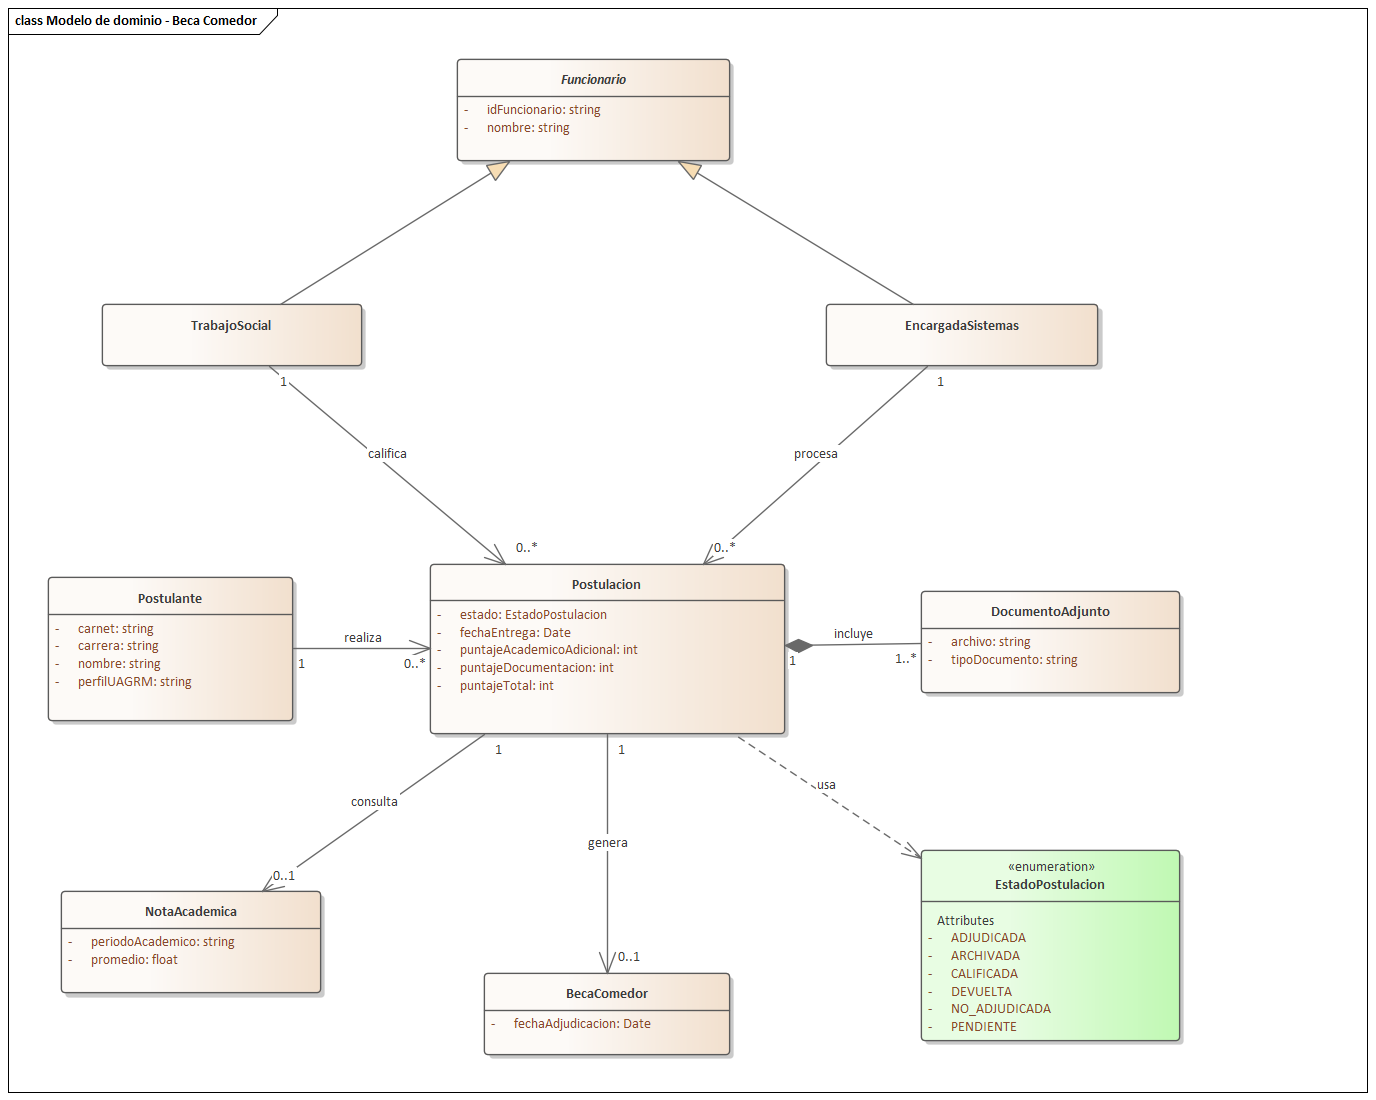
\includegraphics[width=0.9\textwidth,height=0.8\textheight,keepaspectratio]{images/018_Modelo_Dominio.png}

\smallskip
\noindent\raggedright\textit{Nota.} Elaboración propia.
\end{figure}

El proceso gira en torno a la clase \textit{Postulación}, que agrupa la información generada durante todo el trámite: la fecha de entrega de documentación, el puntaje asignado por la revisión documental (1 a 70 puntos), el puntaje adicional otorgado según el rendimiento académico (hasta 30 puntos), el puntaje total resultante, y su estado actual dentro del flujo. Este estado está formalmente restringido a un conjunto cerrado de valores —pendiente, devuelta, archivada, calificada, adjudicada o no adjudicada—, representados mediante la enumeración \textit{EstadoPostulacion}, lo que evita que el sistema admita estados no contemplados en el proceso.

Cada postulación es iniciada por un \textit{Postulante}, identificado por su nombre, carné de identidad, carrera y perfil institucional UAGRM. Un postulante puede generar más de una postulación a lo largo del tiempo —por ejemplo, si su documentación es devuelta y debe corregirla y volver a presentarla—, por lo que la relación entre ambas clases es de uno a muchos.

Toda postulación incluye, de manera obligatoria, uno o más \textit{DocumentoAdjunto}, cada uno caracterizado por su tipo y el archivo correspondiente. Esta relación se modela como una composición, ya que los documentos no tienen existencia ni sentido fuera de la postulación a la que pertenecen: si la postulación se elimina, sus documentos se eliminan con ella.

En el proceso intervienen dos roles de personal administrativo, representados como especializaciones de una clase abstracta común \textit{Funcionario}, que concentra los atributos compartidos de identificador y nombre. El primer rol, \textit{TrabajoSocial}, es responsable de revisar la documentación entregada y calificar la postulación; el segundo, \textit{EncargadaSistemas}, procesa esa calificación, consulta el rendimiento académico del postulante en \textit{NotaAcademica} —registro identificado por período académico y promedio— y calcula el puntaje total que determina la adjudicación.

Cuando el puntaje total alcanza el mínimo requerido, la postulación genera una \textit{BecaComedor}, entidad que registra la fecha de adjudicación. Esta relación es opcional desde la perspectiva de la postulación, ya que no toda postulación calificada llega a adjudicarse.

En conjunto, el modelo refleja que la postulación es el eje central del dominio: nace de un postulante, se sustenta en documentos que le pertenecen exclusivamente, es intervenida por dos roles funcionales distintos en etapas sucesivas del proceso, se apoya en un registro académico externo para el cálculo del puntaje, y —de cumplirse las condiciones— culmina en la adjudicación del beneficio.

% ------------------------------------------------------------------------------
% 4.3. REQUISITOS ESPECÍFICOS
% ------------------------------------------------------------------------------
\subsection{4.3. Requisitos Específicos}\label{sec:ieee_requisitos_especificos}

\subsubsection{4.3.1. Requisitos Funcionales}\label{sec:ieee_rf}
% [INSTRUCCIÓN]: Especificación formal de cada requisito funcional (RF-01, RF-02, etc.).

A continuación se detallan los requisitos funcionales identificados para el sistema, formulados bajo el esquema de historia de usuario (¿quién?, ¿qué? y ¿por qué?) y acompañados de sus respectivos criterios de aceptación. Las Tablas~\ref{tab:rf01} a~\ref{tab:rf21} presentan cada uno de estos requisitos.

% RF-01 no cabe en una página: se usa longtable (mismo encabezado manual que
% las tablas largas del Cap. 5) para que los criterios continúen en la siguiente.
\refstepcounter{table}\label{tab:rf01}
\addcontentsline{lot}{table}{\protect\numberline{\thetable}Requerimiento funcional RF-01: Registro y autenticación de usuarios}
\noindent\textbf{Tabla~\thetable}\par\nopagebreak
\noindent\textit{Requerimiento funcional RF-01: Registro y autenticación de usuarios}\par\nopagebreak
\begingroup
\setlength{\LTleft}{0pt}\setlength{\LTright}{\fill}
\begin{longtable}{>{\raggedright\arraybackslash}p{3.2cm} >{\raggedright\arraybackslash}p{9.3cm}}
\toprule
¿Quién? & Postulante, Administrador DUBSS, Directivo DUBSS y Personal del Comedor Universitario. \\
¿Qué? & Quiere registrarse (el Postulante), autenticarse y cerrar su sesión en el sistema desde el portal web o la aplicación móvil. \\
¿Por qué? & Para acceder de forma segura a las funcionalidades correspondientes a su rol, verificado por el propio sistema mediante un token de acceso firmado. \\
\midrule
\multicolumn{2}{l}{\textbf{Criterios de aceptación}} \\
\multicolumn{2}{p{\dimexpr12.5cm+2\tabcolsep\relax}}{
\begin{itemize}
    \item El sistema permite al Postulante crear una cuenta, y a todo usuario autenticarse y cerrar sesión, desde la web y desde la aplicación móvil. La cuenta creada por autorregistro siempre tiene el rol Postulante; las cuentas del personal las crea el Administrador DUBSS.
\end{itemize}
} \\
\multicolumn{2}{p{\dimexpr12.5cm+2\tabcolsep\relax}}{
\begin{itemize}
    \item El sistema exige que el CI, el registro universitario (9 dígitos numéricos, sin comenzar por 0) y el correo electrónico sean únicos, y que la contraseña tenga al menos 6 caracteres y coincida con su confirmación.
\end{itemize}
} \\
\multicolumn{2}{p{\dimexpr12.5cm+2\tabcolsep\relax}}{
\begin{itemize}
    \item El sistema identifica el rol del usuario autenticado (Postulante, Administrador DUBSS, Directivo o Personal del Comedor) y lo redirige al módulo correspondiente.
\end{itemize}
} \\
\multicolumn{2}{p{\dimexpr12.5cm+2\tabcolsep\relax}}{
\begin{itemize}
    \item El sistema rechaza credenciales inválidas con un mismo mensaje de error, sin revelar si el correo existe, y niega el acceso a las cuentas desactivadas.
\end{itemize}
} \\
\multicolumn{2}{p{\dimexpr12.5cm+2\tabcolsep\relax}}{
\begin{itemize}
    \item El sistema bloquea temporalmente el acceso tras varios intentos fallidos consecutivos (5 intentos y un primer bloqueo de 5 minutos, mayor si se continúa fallando); el bloqueo lo aplica el propio sistema y su escala exacta está por definir con la DUBSS.
\end{itemize}
} \\
\multicolumn{2}{p{\dimexpr12.5cm+2\tabcolsep\relax}}{
\begin{itemize}
    \item El sistema cierra la sesión únicamente en el dispositivo desde el que se solicita, sin afectar las sesiones abiertas en otros dispositivos, y no permite ver pantallas privadas hasta un nuevo inicio de sesión.
\end{itemize}
} \\
\multicolumn{2}{p{\dimexpr12.5cm+2\tabcolsep\relax}}{
\begin{itemize}
    \item El sistema almacena las contraseñas únicamente como hash (nunca en texto plano), no las escribe, junto con los tokens de sesión, en sus registros, y anota en la bitácora cada inicio de sesión exitoso.
\end{itemize}
} \\
\multicolumn{2}{p{\dimexpr12.5cm+2\tabcolsep\relax}}{
\begin{itemize}
    \item El sistema mantiene la sesión mediante un token de acceso de vida corta y un token de renovación por dispositivo, que se guarda solo como hash y se revoca al cerrar sesión.
\end{itemize}
} \\
\bottomrule
\end{longtable}
\endgroup
\addtocounter{table}{-1}
\vspace{-0.5\baselineskip}
\noindent\textit{Nota.} Elaboración propia.\par\medskip

\begin{table}[H]
\caption{Requerimiento funcional RF-02: Envío de postulación a la Beca Comedor}
\label{tab:rf02}
\begin{threeparttable}
\begin{tabular}{>{\raggedright\arraybackslash}p{3.2cm} >{\raggedright\arraybackslash}p{9.3cm}}
\toprule
¿Quién? & Postulante. \\
¿Qué? & Quiere completar un formulario socioeconómico digital y adjuntar la documentación de respaldo digitalizada, desde el portal web o la aplicación móvil. \\
¿Por qué? & Para iniciar formalmente su proceso de postulación a la Beca Comedor. \\
\midrule
\multicolumn{2}{l}{\textbf{Criterios de aceptación}} \\
\multicolumn{2}{p{12.5cm}}{
\begin{itemize}
    \item El Postulante puede completar la totalidad de los campos del formulario socioeconómico.
    \item El Postulante puede adjuntar uno o más archivos digitales como respaldo documental.
    \item El sistema no permite enviar la postulación si falta algún campo o documento obligatorio.
    \item El sistema confirma la recepción de la postulación y la asocia a la gestión académica vigente.
\end{itemize}
} \\
\bottomrule
\end{tabular}
\begin{tablenotes}
\item \textit{Nota.} Elaboración propia.
\end{tablenotes}
\end{threeparttable}
\end{table}

\begin{table}[H]
\caption{Requerimiento funcional RF-03: Preselección automatizada con Inteligencia Artificial}
\label{tab:rf03}
\begin{threeparttable}
\begin{tabular}{>{\raggedright\arraybackslash}p{3.2cm} >{\raggedright\arraybackslash}p{9.3cm}}
\toprule
¿Quién? & Sistema (módulo de preselección con Inteligencia Artificial). \\
¿Qué? & Quiere precalificar automáticamente cada postulación recibida mediante un modelo de inteligencia artificial que evalúe las variables socioeconómicas y académicas declaradas. \\
¿Por qué? & Para generar un puntaje de vulnerabilidad que permita ordenar objetivamente a los postulantes según su nivel de necesidad, sin intervención manual sobre el total de solicitudes recibidas (hasta 20,000 o más por gestión). \\
\midrule
\multicolumn{2}{l}{\textbf{Criterios de aceptación}} \\
\multicolumn{2}{p{12.5cm}}{
\begin{itemize}
    \item El sistema calcula un puntaje de vulnerabilidad para cada postulación dentro de un tiempo razonable tras su envío.
    \item El sistema procesa automáticamente la totalidad de las postulaciones recibidas, sin requerir revisión manual previa.
    \item El sistema registra el puntaje obtenido y la fecha de cálculo, permitiendo su trazabilidad posterior.
\end{itemize}
} \\
\bottomrule
\end{tabular}
\begin{tablenotes}
\item \textit{Nota.} Elaboración propia.
\end{tablenotes}
\end{threeparttable}
\end{table}

\begin{table}[H]
\caption{Requerimiento funcional RF-04: Panel de monitoreo y toma de decisiones (auditoría y adjudicación)}
\label{tab:rf04}
\begin{threeparttable}
\begin{tabular}{>{\raggedright\arraybackslash}p{3.2cm} >{\raggedright\arraybackslash}p{9.3cm}}
\toprule
¿Quién? & Administrador DUBSS. \\
¿Qué? & Quiere visualizar la lista priorizada de postulantes según su puntaje de vulnerabilidad, auditar los expedientes finalistas y aprobar o rechazar la adjudicación de la beca. \\
¿Por qué? & Para validar los expedientes físicos de los finalistas y generar las actas o comprobantes correspondientes a los beneficiarios aprobados. \\
\midrule
\multicolumn{2}{l}{\textbf{Criterios de aceptación}} \\
\multicolumn{2}{p{12.5cm}}{
\begin{itemize}
    \item El Administrador visualiza la lista de postulantes ordenada de mayor a menor puntaje de vulnerabilidad.
    \item El Administrador puede marcar un expediente como auditado o validado tras revisar el respaldo físico.
    \item El Administrador puede aprobar o rechazar la adjudicación de la beca para cada postulante auditado.
    \item El sistema genera un acta o comprobante digital de adjudicación para cada beneficiario aprobado.
\end{itemize}
} \\
\bottomrule
\end{tabular}
\begin{tablenotes}
\item \textit{Nota.} Elaboración propia.
\end{tablenotes}
\end{threeparttable}
\end{table}

\begin{table}[H]
\caption{Requerimiento funcional RF-05: Registro e impresión de planillas de asistencia}
\label{tab:rf05}
\begin{threeparttable}
\begin{tabular}{>{\raggedright\arraybackslash}p{3.2cm} >{\raggedright\arraybackslash}p{9.3cm}}
\toprule
¿Quién? & Administrador DUBSS y personal del Comedor Universitario. \\
¿Qué? & Quiere generar planillas de asistencia física y digital para su firma y fotocopia de carnet, y registrar digitalmente la asistencia diaria ya verificada de los becados. \\
¿Por qué? & Para mantener un respaldo cruzable frente a las auditorías externas, sin que el sistema dependa de ningún dispositivo de identificación biométrica propio, dado que dicha verificación física es responsabilidad de la empresa concesionaria. \\
\midrule
\multicolumn{2}{l}{\textbf{Criterios de aceptación}} \\
\multicolumn{2}{p{12.5cm}}{
\begin{itemize}
    \item El sistema genera planillas de asistencia imprimibles, listas para firma física y fotocopia de carnet.
    \item El sistema permite registrar digitalmente la asistencia diaria de cada becario, una vez verificada su identidad por el personal del comedor.
    \item El sistema permite cotejar el registro digital de asistencia contra el respaldo físico (planilla firmada) durante una auditoría.
    \item El sistema no depende de ningún dispositivo de identificación biométrica propio; esa verificación es externa al sistema.
\end{itemize}
} \\
\bottomrule
\end{tabular}
\begin{tablenotes}
\item \textit{Nota.} Elaboración propia.
\end{tablenotes}
\end{threeparttable}
\end{table}

\begin{table}[H]
\caption{Requerimiento funcional RF-06: Consultas y notificaciones al postulante}
\label{tab:rf06}
\begin{threeparttable}
\begin{tabular}{>{\raggedright\arraybackslash}p{3.2cm} >{\raggedright\arraybackslash}p{9.3cm}}
\toprule
¿Quién? & Postulante. \\
¿Qué? & Quiere realizar seguimiento en tiempo real del estado de su postulación (recibida, en evaluación, finalista, adjudicada, rechazada) y recibir notificaciones push sobre eventos relevantes. \\
¿Por qué? & Para mantenerse informado del avance y del resultado de su beneficio sin necesidad de acudir presencialmente a la DUBSS. \\
\midrule
\multicolumn{2}{l}{\textbf{Criterios de aceptación}} \\
\multicolumn{2}{p{12.5cm}}{
\begin{itemize}
    \item El Postulante puede consultar en todo momento el estado actual de su postulación.
    \item El sistema notifica automáticamente al Postulante cuando su estado cambia (por ejemplo, al ser seleccionado como finalista o al adjudicársele la beca).
\end{itemize}
} \\
\bottomrule
\end{tabular}
\begin{tablenotes}
\item \textit{Nota.} Elaboración propia.
\end{tablenotes}
\end{threeparttable}
\end{table}

\begin{table}[H]
\caption{Requerimiento funcional RF-07: Dashboard de indicadores de Business Intelligence}
\label{tab:rf07}
\begin{threeparttable}
\begin{tabular}{>{\raggedright\arraybackslash}p{3.2cm} >{\raggedright\arraybackslash}p{9.3cm}}
\toprule
¿Quién? & Directivo DUBSS. \\
¿Qué? & Quiere visualizar un dashboard interactivo de Business Intelligence con indicadores clave del comportamiento histórico de las postulaciones y del uso del beneficio. \\
¿Por qué? & Para apoyar la planificación institucional y la rendición de cuentas con información consolidada de cada gestión. \\
\midrule
\multicolumn{2}{l}{\textbf{Criterios de aceptación}} \\
\multicolumn{2}{p{12.5cm}}{
\begin{itemize}
    \item El Directivo puede visualizar indicadores clave (postulaciones recibidas, becas adjudicadas, asistencia) en un dashboard interactivo.
    \item El sistema permite filtrar los indicadores por gestión académica.
\end{itemize}
} \\
\bottomrule
\end{tabular}
\begin{tablenotes}
\item \textit{Nota.} Elaboración propia.
\end{tablenotes}
\end{threeparttable}
\end{table}

\begin{table}[H]
\caption{Requerimiento funcional RF-08: Gestión de convocatorias y gestiones académicas}
\label{tab:rf08}
\begin{threeparttable}
\begin{tabular}{>{\raggedright\arraybackslash}p{3.2cm} >{\raggedright\arraybackslash}p{9.3cm}}
\toprule
¿Quién? & Administrador DUBSS. \\
¿Qué? & Quiere crear, editar, abrir y cerrar convocatorias de la Beca Comedor, definiendo la gestión académica, las fechas, el número de cupos y los documentos requeridos. \\
¿Por qué? & Para controlar el periodo en que se reciben postulaciones y asociar cada postulación a la gestión vigente. \\
\midrule
\multicolumn{2}{l}{\textbf{Criterios de aceptación}} \\
\multicolumn{2}{p{12.5cm}}{
\begin{itemize}
    \item El Administrador puede registrar una convocatoria con gestión académica, fecha de apertura, fecha de cierre y cupos (por definir con la DUBSS).
    \item El Administrador puede definir la lista de documentos obligatorios de cada convocatoria.
    \item El sistema solo permite enviar postulaciones mientras la convocatoria esté abierta.
    \item Solo puede existir una convocatoria vigente por gestión académica.
\end{itemize}
} \\
\bottomrule
\end{tabular}
\begin{tablenotes}
\item \textit{Nota.} Elaboración propia.
\end{tablenotes}
\end{threeparttable}
\end{table}

\begin{table}[H]
\caption{Requerimiento funcional RF-09: Gestión de usuarios y roles}
\label{tab:rf09}
\begin{threeparttable}
\begin{tabular}{>{\raggedright\arraybackslash}p{3.2cm} >{\raggedright\arraybackslash}p{9.3cm}}
\toprule
¿Quién? & Administrador DUBSS. \\
¿Qué? & Quiere crear, editar, desactivar y asignar roles (Administrador, Directivo y Personal del Comedor) a las cuentas del personal. \\
¿Por qué? & Para garantizar que cada persona acceda únicamente a las funciones de su rol, conforme al control de acceso exigido por el sistema. \\
\midrule
\multicolumn{2}{l}{\textbf{Criterios de aceptación}} \\
\multicolumn{2}{p{12.5cm}}{
\begin{itemize}
    \item El Administrador puede crear y desactivar cuentas de personal y asignarles un rol.
    \item El sistema impide que un usuario acceda a funciones de un rol distinto al asignado.
    \item El sistema conserva el registro de los cambios de rol realizados.
    \item El sistema rechaza el alta de una cuenta con CI o correo electrónico ya registrados.
\end{itemize}
} \\
\bottomrule
\end{tabular}
\begin{tablenotes}
\item \textit{Nota.} Elaboración propia.
\end{tablenotes}
\end{threeparttable}
\end{table}

\begin{table}[H]
\caption{Requerimiento funcional RF-10: Recuperación de contraseña y gestión de perfil}
\label{tab:rf10}
\begin{threeparttable}
\begin{tabular}{>{\raggedright\arraybackslash}p{3.2cm} >{\raggedright\arraybackslash}p{9.3cm}}
\toprule
¿Quién? & Postulante, Administrador DUBSS, Directivo DUBSS y Personal del Comedor Universitario. \\
¿Qué? & Quiere recuperar su contraseña en caso de olvido y actualizar sus datos de contacto desde su perfil. \\
¿Por qué? & Para recuperar el acceso a su cuenta sin intervención del personal y mantener actualizados los datos con que se le notifica. \\
\midrule
\multicolumn{2}{l}{\textbf{Criterios de aceptación}} \\
\multicolumn{2}{p{12.5cm}}{
\begin{itemize}
    \item El usuario puede solicitar el restablecimiento de contraseña mediante un enlace enviado a su correo registrado, gestionado por el propio sistema.
    \item El usuario puede modificar sus datos de contacto y su contraseña desde el perfil.
    \item El sistema no permite modificar el CI desde el perfil.
\end{itemize}
} \\
\bottomrule
\end{tabular}
\begin{tablenotes}
\item \textit{Nota.} Elaboración propia.
\end{tablenotes}
\end{threeparttable}
\end{table}

\begin{table}[H]
\caption{Requerimiento funcional RF-11: Digitalización y carga de documentos de respaldo}
\label{tab:rf11}
\begin{threeparttable}
\begin{tabular}{>{\raggedright\arraybackslash}p{3.2cm} >{\raggedright\arraybackslash}p{9.3cm}}
\toprule
¿Quién? & Postulante. \\
¿Qué? & Quiere digitalizar sus documentos con la cámara del teléfono, o cargarlos desde un archivo en la web, y asociarlos a su postulación. \\
¿Por qué? & Para respaldar los datos declarados en el formulario socioeconómico sin presentar carpetas físicas en la etapa inicial. \\
\midrule
\multicolumn{2}{l}{\textbf{Criterios de aceptación}} \\
\multicolumn{2}{p{12.5cm}}{
\begin{itemize}
    \item El Postulante puede capturar un documento con la cámara del dispositivo móvil o adjuntar un archivo desde la web.
    \item El sistema valida el formato y el tamaño del archivo (formatos y tamaño máximo por definir con la DUBSS) y rechaza los no permitidos con un mensaje de error.
    \item El sistema muestra una vista previa y permite reemplazar o eliminar un documento antes de enviar la postulación.
    \item El sistema almacena los archivos en Firebase Storage asociados a la postulación.
\end{itemize}
} \\
\bottomrule
\end{tabular}
\begin{tablenotes}
\item \textit{Nota.} Elaboración propia.
\end{tablenotes}
\end{threeparttable}
\end{table}

\begin{table}[H]
\caption{Requerimiento funcional RF-12: Guardado de borrador de postulación}
\label{tab:rf12}
\begin{threeparttable}
\begin{tabular}{>{\raggedright\arraybackslash}p{3.2cm} >{\raggedright\arraybackslash}p{9.3cm}}
\toprule
¿Quién? & Postulante. \\
¿Qué? & Quiere guardar su postulación incompleta como borrador y retomarla después. \\
¿Por qué? & Para completar el formulario socioeconómico y reunir los documentos sin perder lo ya ingresado. \\
\midrule
\multicolumn{2}{l}{\textbf{Criterios de aceptación}} \\
\multicolumn{2}{p{12.5cm}}{
\begin{itemize}
    \item El Postulante puede guardar el formulario con campos obligatorios sin completar.
    \item El Postulante puede retomar y editar el borrador mientras la convocatoria esté abierta.
    \item Un borrador no se considera enviado ni es procesado por el módulo de preselección.
    \item El sistema descarta o bloquea los borradores no enviados al cerrar la convocatoria.
\end{itemize}
} \\
\bottomrule
\end{tabular}
\begin{tablenotes}
\item \textit{Nota.} Elaboración propia.
\end{tablenotes}
\end{threeparttable}
\end{table}

\begin{table}[H]
\caption{Requerimiento funcional RF-13: Validación de elegibilidad y unicidad de postulaciones}
\label{tab:rf13}
\begin{threeparttable}
\begin{tabular}{>{\raggedright\arraybackslash}p{3.2cm} >{\raggedright\arraybackslash}p{9.3cm}}
\toprule
¿Quién? & Sistema. \\
¿Qué? & Quiere verificar, al recibir una postulación, que el postulante cumple las condiciones de elegibilidad y que no existe otra postulación suya en la misma gestión. \\
¿Por qué? & Para evitar registros duplicados o inválidos que distorsionen la priorización y la adjudicación. \\
\midrule
\multicolumn{2}{l}{\textbf{Criterios de aceptación}} \\
\multicolumn{2}{p{12.5cm}}{
\begin{itemize}
    \item El sistema impide enviar más de una postulación vigente por postulante y por convocatoria.
    \item El sistema verifica las condiciones de elegibilidad (por definir con la DUBSS) antes de aceptar el envío.
    \item El sistema informa al Postulante el motivo cuando su postulación es rechazada por esta validación.
    \item Una postulación devuelta (RF-14) y reenviada no se considera duplicada.
\end{itemize}
} \\
\bottomrule
\end{tabular}
\begin{tablenotes}
\item \textit{Nota.} Elaboración propia.
\end{tablenotes}
\end{threeparttable}
\end{table}

\begin{table}[H]
\caption{Requerimiento funcional RF-14: Devolución de postulación para corrección}
\label{tab:rf14}
\begin{threeparttable}
\begin{tabular}{>{\raggedright\arraybackslash}p{3.2cm} >{\raggedright\arraybackslash}p{9.3cm}}
\toprule
¿Quién? & Administrador DUBSS (y Postulante, como receptor). \\
¿Qué? & Quiere devolver una postulación con observaciones para que el Postulante corrija o complete su documentación y la reenvíe. \\
¿Por qué? & Para evitar descartar postulaciones por defectos subsanables y mantener la trazabilidad de las correcciones. \\
\midrule
\multicolumn{2}{l}{\textbf{Criterios de aceptación}} \\
\multicolumn{2}{p{12.5cm}}{
\begin{itemize}
    \item El Administrador puede devolver una postulación registrando las observaciones.
    \item La postulación cambia al estado devuelta y el Postulante es notificado.
    \item El Postulante puede corregir y reenviar dentro de un plazo (por definir con la DUBSS).
    \item El sistema conserva el historial de devoluciones y reenvíos de la postulación.
\end{itemize}
} \\
\bottomrule
\end{tabular}
\begin{tablenotes}
\item \textit{Nota.} Elaboración propia.
\end{tablenotes}
\end{threeparttable}
\end{table}

\begin{table}[H]
\caption{Requerimiento funcional RF-15: Archivo o rechazo de postulación}
\label{tab:rf15}
\begin{threeparttable}
\begin{tabular}{>{\raggedright\arraybackslash}p{3.2cm} >{\raggedright\arraybackslash}p{9.3cm}}
\toprule
¿Quién? & Administrador DUBSS. \\
¿Qué? & Quiere archivar o rechazar una postulación indicando el motivo. \\
¿Por qué? & Para cerrar formalmente los expedientes que no proceden y dejar constancia de la decisión. \\
\midrule
\multicolumn{2}{l}{\textbf{Criterios de aceptación}} \\
\multicolumn{2}{p{12.5cm}}{
\begin{itemize}
    \item El Administrador debe registrar un motivo para archivar o rechazar.
    \item La postulación pasa al estado correspondiente (archivada o no adjudicada) y deja de aparecer en la lista priorizada activa.
    \item El Postulante puede ver el estado y el motivo registrado.
    \item El sistema conserva la postulación archivada para consulta histórica y reportes.
\end{itemize}
} \\
\bottomrule
\end{tabular}
\begin{tablenotes}
\item \textit{Nota.} Elaboración propia.
\end{tablenotes}
\end{threeparttable}
\end{table}

\begin{table}[H]
\caption{Requerimiento funcional RF-16: Notificación a finalistas, entrega de documentación física y comunicados}
\label{tab:rf16}
\begin{threeparttable}
\begin{tabular}{>{\raggedright\arraybackslash}p{3.2cm} >{\raggedright\arraybackslash}p{9.3cm}}
\toprule
¿Quién? & Administrador DUBSS (y Postulante, como receptor). \\
¿Qué? & Quiere notificar a los finalistas para que presenten su documentación física, registrar la fecha en que se recibe, y publicar comunicados y avisos generales dirigidos a postulantes. \\
¿Por qué? & Para coordinar la auditoría física de los finalistas, dejar constancia de su entrega y mantener informada a la población postulante. \\
\midrule
\multicolumn{2}{l}{\textbf{Criterios de aceptación}} \\
\multicolumn{2}{p{12.5cm}}{
\begin{itemize}
    \item El sistema envía una notificación push a cada finalista indicando el plazo y los documentos que debe presentar.
    \item El Administrador puede registrar la recepción de la documentación física de un finalista con su fecha.
    \item El Administrador puede publicar un comunicado dirigido a todos los postulantes o a un grupo (por ejemplo, los finalistas).
    \item Los comunicados se notifican mediante push y quedan consultables desde la aplicación.
\end{itemize}
} \\
\bottomrule
\end{tabular}
\begin{tablenotes}
\item \textit{Nota.} Elaboración propia.
\end{tablenotes}
\end{threeparttable}
\end{table}

\begin{table}[H]
\caption{Requerimiento funcional RF-17: Publicación de resultados de adjudicación}
\label{tab:rf17}
\begin{threeparttable}
\begin{tabular}{>{\raggedright\arraybackslash}p{3.2cm} >{\raggedright\arraybackslash}p{9.3cm}}
\toprule
¿Quién? & Administrador DUBSS. \\
¿Qué? & Quiere publicar la lista oficial de adjudicados de la gestión. \\
¿Por qué? & Para dar a conocer los resultados de forma transparente y oficial y poner fin al proceso de selección. \\
\midrule
\multicolumn{2}{l}{\textbf{Criterios de aceptación}} \\
\multicolumn{2}{p{12.5cm}}{
\begin{itemize}
    \item El Administrador puede publicar los resultados solo cuando todas las adjudicaciones estén decididas.
    \item La lista publicada incluye a los adjudicados de la gestión y es consultable por los postulantes.
    \item Al publicar, el sistema notifica a cada postulante su resultado.
    \item Una vez publicada, la lista no se modifica sin dejar registro en la bitácora (RF-20).
\end{itemize}
} \\
\bottomrule
\end{tabular}
\begin{tablenotes}
\item \textit{Nota.} Elaboración propia.
\end{tablenotes}
\end{threeparttable}
\end{table}

\begin{table}[H]
\caption{Requerimiento funcional RF-18: Gestión del padrón de becados}
\label{tab:rf18}
\begin{threeparttable}
\begin{tabular}{>{\raggedright\arraybackslash}p{3.2cm} >{\raggedright\arraybackslash}p{9.3cm}}
\toprule
¿Quién? & Administrador DUBSS. \\
¿Qué? & Quiere mantener el padrón de becados vigentes, registrando bajas, suspensiones y reemplazos durante la gestión. \\
¿Por qué? & Para mantener actualizada la lista de beneficiarios activos, de la cual dependen las planillas de asistencia, y reasignar los cupos liberados. \\
\midrule
\multicolumn{2}{l}{\textbf{Criterios de aceptación}} \\
\multicolumn{2}{p{12.5cm}}{
\begin{itemize}
    \item El Administrador puede consultar el padrón de becados vigentes de la gestión.
    \item El Administrador puede dar de baja o suspender a un becado registrando el motivo.
    \item El Administrador puede reemplazar un cupo liberado con el siguiente postulante priorizado.
    \item Los cambios en el padrón se reflejan en las planillas de asistencia generadas posteriormente.
\end{itemize}
} \\
\bottomrule
\end{tabular}
\begin{tablenotes}
\item \textit{Nota.} Elaboración propia.
\end{tablenotes}
\end{threeparttable}
\end{table}

\begin{table}[H]
\caption{Requerimiento funcional RF-19: Historial de asistencia y estado de la beca}
\label{tab:rf19}
\begin{threeparttable}
\begin{tabular}{>{\raggedright\arraybackslash}p{3.2cm} >{\raggedright\arraybackslash}p{9.3cm}}
\toprule
¿Quién? & Becado (Postulante adjudicado). \\
¿Qué? & Quiere consultar su historial de asistencia al comedor y el estado vigente de su beca. \\
¿Por qué? & Para verificar su cumplimiento de los requisitos de asistencia y conservar su beneficio. \\
\midrule
\multicolumn{2}{l}{\textbf{Criterios de aceptación}} \\
\multicolumn{2}{p{12.5cm}}{
\begin{itemize}
    \item El Becado visualiza las fechas de asistencia registradas en la gestión vigente.
    \item El Becado visualiza el estado de su beca (vigente, suspendida o dada de baja) y el motivo, si corresponde.
    \item El Becado solo accede a su propia información.
\end{itemize}
} \\
\bottomrule
\end{tabular}
\begin{tablenotes}
\item \textit{Nota.} Elaboración propia.
\end{tablenotes}
\end{threeparttable}
\end{table}

\begin{table}[H]
\caption{Requerimiento funcional RF-20: Bitácora de acciones}
\label{tab:rf20}
\begin{threeparttable}
\begin{tabular}{>{\raggedright\arraybackslash}p{3.2cm} >{\raggedright\arraybackslash}p{9.3cm}}
\toprule
¿Quién? & Administrador DUBSS. \\
¿Qué? & Quiere consultar un registro de las acciones relevantes realizadas en el sistema (auditoría, devolución, adjudicación, cambios en el padrón y cambios de roles). \\
¿Por qué? & Para garantizar la trazabilidad de las decisiones y facilitar las auditorías sobre el proceso. \\
\midrule
\multicolumn{2}{l}{\textbf{Criterios de aceptación}} \\
\multicolumn{2}{p{12.5cm}}{
\begin{itemize}
    \item El sistema registra automáticamente usuario, acción, expediente afectado, fecha y hora.
    \item El Administrador puede filtrar la bitácora por usuario, tipo de acción y rango de fechas.
    \item Los registros de la bitácora no pueden ser editados ni eliminados desde la interfaz.
\end{itemize}
} \\
\bottomrule
\end{tabular}
\begin{tablenotes}
\item \textit{Nota.} Elaboración propia.
\end{tablenotes}
\end{threeparttable}
\end{table}

\begin{table}[H]
\caption{Requerimiento funcional RF-21: Parametrización del modelo de preselección y reprocesamiento}
\label{tab:rf21}
\begin{threeparttable}
\begin{tabular}{>{\raggedright\arraybackslash}p{3.2cm} >{\raggedright\arraybackslash}p{9.3cm}}
\toprule
¿Quién? & Administrador DUBSS. \\
¿Qué? & Quiere ajustar los criterios y ponderaciones que usa el modelo de preselección y reprocesar los puntajes de las postulaciones de una convocatoria. \\
¿Por qué? & Para calibrar la priorización según los criterios institucionales de vulnerabilidad y corregir puntajes cuando estos cambien. \\
\midrule
\multicolumn{2}{l}{\textbf{Criterios de aceptación}} \\
\multicolumn{2}{p{12.5cm}}{
\begin{itemize}
    \item El Administrador puede consultar y modificar los criterios y ponderaciones del modelo (por definir con la DUBSS).
    \item El Administrador puede solicitar el reprocesamiento de los puntajes de una convocatoria.
    \item El sistema registra la fecha de cada recálculo y conserva el puntaje anterior para trazabilidad (ver RF-03).
    \item El sistema muestra la lista priorizada actualizada tras el reprocesamiento.
\end{itemize}
} \\
\bottomrule
\end{tabular}
\begin{tablenotes}
\item \textit{Nota.} Elaboración propia.
\end{tablenotes}
\end{threeparttable}
\end{table}

\subsubsection{4.3.2. Requisitos No Funcionales}\label{sec:ieee_rnf}
% [INSTRUCCIÓN]: Rendimiento, seguridad, disponibilidad, mantenibilidad y fiabilidad (RNF-01, etc.).

A continuación se detallan los requisitos no funcionales identificados para el sistema, describiendo los atributos de calidad exigidos y sus respectivos criterios de aceptación. Las Tablas~\ref{tab:rnf01} a~\ref{tab:rnf05} presentan cada uno de estos requisitos.

\begin{table}[H]
\caption{Requerimiento no funcional RNF-01: Seguridad y protección de datos personales}
\label{tab:rnf01}
\begin{threeparttable}
\begin{tabular}{>{\raggedright\arraybackslash}p{3.2cm} >{\raggedright\arraybackslash}p{9.3cm}}
\toprule
\multicolumn{2}{l}{\textbf{Descripción}} \\
\multicolumn{2}{p{12.5cm}}{El sistema debe garantizar la confidencialidad, integridad y protección de los datos socioeconómicos y personales de los postulantes, aplicando control de acceso basado en roles y cifrado de la información sensible almacenada y transmitida, en cumplimiento de las políticas institucionales de protección de datos personales de la UAGRM.} \\
\midrule
\multicolumn{2}{l}{\textbf{Criterios de aceptación}} \\
\multicolumn{2}{p{12.5cm}}{
\begin{itemize}
    \item El acceso a los expedientes socioeconómicos está restringido según el rol del usuario autenticado.
    \item La información sensible se transmite y almacena de forma cifrada.
    \item El sistema mantiene un registro (log) de los accesos realizados a cada expediente.
\end{itemize}
} \\
\bottomrule
\end{tabular}
\begin{tablenotes}
\item \textit{Nota.} Elaboración propia.
\end{tablenotes}
\end{threeparttable}
\end{table}

\begin{table}[H]
\caption{Requerimiento no funcional RNF-02: Disponibilidad del servicio}
\label{tab:rnf02}
\begin{threeparttable}
\begin{tabular}{>{\raggedright\arraybackslash}p{3.2cm} >{\raggedright\arraybackslash}p{9.3cm}}
\toprule
\multicolumn{2}{l}{\textbf{Descripción}} \\
\multicolumn{2}{p{12.5cm}}{El sistema debe mantenerse operativo y accesible durante los periodos de alta demanda, particularmente durante las fechas de apertura y cierre de la convocatoria de postulación, minimizando el riesgo de interrupciones del servicio desplegado en AWS.} \\
\midrule
\multicolumn{2}{l}{\textbf{Criterios de aceptación}} \\
\multicolumn{2}{p{12.5cm}}{
\begin{itemize}
    \item El portal web y la aplicación móvil permanecen disponibles durante los picos de postulación.
    \item El sistema cuenta con un mecanismo de recuperación ante caídas del servidor.
\end{itemize}
} \\
\bottomrule
\end{tabular}
\begin{tablenotes}
\item \textit{Nota.} Elaboración propia.
\end{tablenotes}
\end{threeparttable}
\end{table}

\begin{table}[H]
\caption{Requerimiento no funcional RNF-03: Tiempo de respuesta y concurrencia}
\label{tab:rnf03}
\begin{threeparttable}
\begin{tabular}{>{\raggedright\arraybackslash}p{3.2cm} >{\raggedright\arraybackslash}p{9.3cm}}
\toprule
\multicolumn{2}{l}{\textbf{Descripción}} \\
\multicolumn{2}{p{12.5cm}}{El sistema debe procesar la precalificación automática y las operaciones de consulta dentro de tiempos de respuesta aceptables, incluso bajo condiciones de alta concurrencia, considerando el volumen de hasta 20,000 postulaciones por gestión y la revisión masiva simultánea por parte de los auditores.} \\
\midrule
\multicolumn{2}{l}{\textbf{Criterios de aceptación}} \\
\multicolumn{2}{p{12.5cm}}{
\begin{itemize}
    \item El algoritmo de precalificación procesa el total de postulaciones dentro de un tiempo máximo a definir mediante pruebas de carga.
    \item El sistema atiende solicitudes concurrentes de múltiples usuarios sin degradar significativamente su rendimiento.
    \item El sistema maneja correctamente peticiones HTTP duplicadas durante la revisión masiva de carpetas, evitando registros o acciones repetidas (idempotencia).
\end{itemize}
} \\
\bottomrule
\end{tabular}
\begin{tablenotes}
\item \textit{Nota.} Elaboración propia.
\end{tablenotes}
\end{threeparttable}
\end{table}

\begin{table}[H]
\caption{Requerimiento no funcional RNF-04: Usabilidad}
\label{tab:rnf04}
\begin{threeparttable}
\begin{tabular}{>{\raggedright\arraybackslash}p{3.2cm} >{\raggedright\arraybackslash}p{9.3cm}}
\toprule
\multicolumn{2}{l}{\textbf{Descripción}} \\
\multicolumn{2}{p{12.5cm}}{El sistema debe ofrecer interfaces simples e intuitivas, acordes al nivel de conocimiento técnico básico de sus usuarios (Postulante, Administrador y Directivo), sin requerir conocimientos de programación para su uso.} \\
\midrule
\multicolumn{2}{l}{\textbf{Criterios de aceptación}} \\
\multicolumn{2}{p{12.5cm}}{
\begin{itemize}
    \item Un usuario sin experiencia previa en el sistema puede completar el flujo de postulación sin asistencia externa.
    \item El panel de reportes del Directivo se interpreta sin necesidad de conocimientos técnicos.
\end{itemize}
} \\
\bottomrule
\end{tabular}
\begin{tablenotes}
\item \textit{Nota.} Elaboración propia.
\end{tablenotes}
\end{threeparttable}
\end{table}

\begin{table}[H]
\caption{Requerimiento no funcional RNF-05: Compatibilidad y restricciones tecnológicas}
\label{tab:rnf05}
\begin{threeparttable}
\begin{tabular}{>{\raggedright\arraybackslash}p{3.2cm} >{\raggedright\arraybackslash}p{9.3cm}}
\toprule
\multicolumn{2}{l}{\textbf{Descripción}} \\
\multicolumn{2}{p{12.5cm}}{El sistema debe cumplir con las restricciones tecnológicas ya definidas para el proyecto: despliegue en un servidor en la nube de AWS, motor de base de datos PostgreSQL, autenticación propia mediante tokens JWT, notificaciones push y almacenamiento de archivos a través de Firebase, y aplicación móvil desarrollada en Flutter con prioridad de compatibilidad para dispositivos Android.} \\
\midrule
\multicolumn{2}{l}{\textbf{Criterios de aceptación}} \\
\multicolumn{2}{p{12.5cm}}{
\begin{itemize}
    \item El backend del sistema se despliega correctamente sobre AWS utilizando PostgreSQL.
    \item La autenticación la resuelve el propio backend mediante tokens JWT, y las notificaciones push y el almacenamiento de archivos operan a través de Firebase.
    \item La aplicación móvil funciona correctamente en dispositivos Android.
\end{itemize}
} \\
\bottomrule
\end{tabular}
\begin{tablenotes}
\item \textit{Nota.} Elaboración propia.
\end{tablenotes}
\end{threeparttable}
\end{table}

\subsubsection{4.3.3. Requisitos de Interfaz}\label{sec:ieee_interfaces}
% [INSTRUCCIÓN]: Directrices de diseño responsivo, accesibilidad y prototipos de pantalla principales.

Los requisitos de interfaz definen cómo el sistema interactúa con sus usuarios, con el hardware disponible y con otros componentes de software, y se organizan en cuatro categorías.

\begin{itemize}
    \item \textbf{Interfaz de usuario:} el portal web debe desarrollarse con React y TypeScript, y la aplicación móvil con Flutter, ambos bajo un diseño responsivo que se adapte a distintos tamaños de pantalla. La interfaz gráfica de la aplicación móvil debe seguir las directrices de \textit{Material Design}, propias del framework Flutter, garantizando coherencia visual y accesibilidad básica (contraste adecuado, tamaños de fuente legibles) para usuarios sin experiencia técnica previa.
    \item \textbf{Interfaz de hardware:} la aplicación móvil debe ser compatible con dispositivos Android de gama media, como los equipos utilizados para las pruebas del proyecto (Redmi Note 14 Pro y Honor X8), y debe permitir el uso de la cámara del dispositivo para la digitalización de documentos de respaldo.
    \item \textbf{Interfaz de software:} el sistema debe exponer e integrar servicios mediante una API REST desarrollada en Spring Boot, que comunique al frontend web y a la aplicación móvil con la base de datos PostgreSQL y con el módulo de preselección desarrollado en Python. Asimismo, debe integrarse con los servicios de Firebase para el almacenamiento de archivos y el envío de notificaciones push.
    \item \textbf{Interfaz de comunicación:} toda transmisión de datos entre los clientes (web y móvil) y el servidor debe realizarse mediante el protocolo HTTPS, y la autenticación de las peticiones debe validarse mediante el token de acceso (JWT) que emite el propio servidor y que este verifica en cada petición, a fin de proteger la información socioeconómica sensible de los postulantes durante su transmisión.
\end{itemize}

\subsubsection{4.3.4. Requisitos de Base de Datos}\label{sec:ieee_requisitos_bd}
% [INSTRUCCIÓN]: Entidades principales, integridad referencial, respaldos y políticas de retención de datos.

Los requisitos de base de datos definen la estructura y las reglas de gestión de los datos del sistema, sin entrar en el diseño detallado de las tablas, el cual corresponde a una etapa posterior del proyecto.

\begin{itemize}
    \item El sistema debe almacenar los registros de usuarios, postulaciones, expedientes, calificaciones de vulnerabilidad y asistencia en una base de datos relacional PostgreSQL.
    \item El campo correspondiente al carnet de identidad (CI) y al correo electrónico debe ser único dentro de la tabla de usuarios, impidiendo el registro de cuentas duplicadas.
    \item Las tablas de postulaciones, expedientes y asistencia deben mantener integridad referencial mediante claves foráneas hacia la tabla de usuarios, evitando registros huérfanos.
    \item La base de datos debe tener capacidad para almacenar, como mínimo, los registros correspondientes a las 20,000 postulaciones recibidas por gestión académica, conservando el histórico de gestiones anteriores para su explotación en los reportes de Business Intelligence.
\end{itemize}

\subsubsection{4.3.5. Restricciones de Diseño}\label{sec:ieee_restricciones_diseno}
% [INSTRUCCIÓN]: Estándares, lenguajes, herramientas o patrones de arquitectura obligatorios para el diseño del sistema.

El diseño e implementación del sistema está sujeto a las siguientes restricciones técnicas y normativas:

\begin{itemize}
    \item El backend debe desarrollarse en el lenguaje Java utilizando el framework Spring Boot, bajo una arquitectura de servicios RESTful.
    \item El frontend web debe desarrollarse con React y TypeScript, y la aplicación móvil con Flutter y el lenguaje Dart.
    \item El módulo de preselección con Inteligencia Artificial debe desarrollarse en Python, como un componente independiente del backend principal, consumido a través de una API.
    \item El control de versiones del código fuente debe llevarse a cabo en GitHub, y los entornos de desarrollo deben estandarizarse mediante contenedores Docker.
    \item El diseño de la Especificación de Requisitos del Software debe ajustarse al estándar IEEE 830, y el manejo de los datos socioeconómicos de los postulantes debe cumplir con las políticas institucionales de protección de datos personales de la UAGRM.
\end{itemize}

\subsubsection{4.3.6. Requisitos de Rendimiento}\label{sec:ieee_requisitos_rendimiento}
% [INSTRUCCIÓN]: Tiempos de respuesta, capacidad de procesamiento, concurrencia y escalabilidad esperados.

\paragraph{4.3.6.1. Tiempo de respuesta.}

\begin{itemize}
    \item La interfaz principal del portal web y de la aplicación móvil no debe tardar más de 3 segundos en cargar bajo condiciones normales de operación.
    \item El sistema debe mostrar la lista priorizada de postulantes al Administrador DUBSS en un tiempo no mayor a 3 segundos.
    \item El cálculo del puntaje de vulnerabilidad de una postulación individual no debe exceder los 5 segundos desde su envío.
\end{itemize}

\paragraph{4.3.6.2. Capacidad y carga máxima.}

\begin{itemize}
    \item El sistema debe procesar la totalidad de las postulaciones recibidas por gestión (hasta 20,000) sin degradar su rendimiento.
    \item El sistema debe soportar al menos 50 usuarios administrativos concurrentes durante la fase de auditoría de expedientes, sin afectar el tiempo de respuesta.
\end{itemize}

\paragraph{4.3.6.3. Uso de recursos (CPU, memoria y ancho de banda).}

\begin{itemize}
    \item El servidor desplegado en AWS no debe superar el 80\% de uso de CPU ni de memoria durante los picos de carga esperados (apertura y cierre de la convocatoria).
    \item El consumo de ancho de banda de un usuario concurrente no debe degradar de forma perceptible la experiencia de otros usuarios conectados simultáneamente.
\end{itemize}

\paragraph{4.3.6.4. Disponibilidad y tiempo de actividad (\textit{uptime}).}

\begin{itemize}
    \item El sistema debe garantizar una disponibilidad mínima del 99\% durante los periodos de postulación y evaluación de cada gestión académica.
    \item Los mantenimientos o actualizaciones programadas deben realizarse fuera del horario de atención administrativa de la DUBSS.
\end{itemize}

\paragraph{4.3.6.5. Escalabilidad.}

\begin{itemize}
    \item La arquitectura del sistema debe permitir el incremento del volumen de postulaciones en gestiones futuras sin requerir un rediseño estructural.
    \item El backend debe poder escalar mediante la incorporación de instancias adicionales en AWS conforme crezca la demanda del servicio.
\end{itemize}

\paragraph{4.3.6.6. Procesamiento en lote o en tiempo real.}

\begin{itemize}
    \item La autenticación, el envío de postulaciones y la consulta del estado de la beca deben procesarse en tiempo real.
    \item La generación de los reportes y dashboards de Business Intelligence puede procesarse en lotes programados (por ejemplo, de forma diaria o al cierre de la gestión), sin requerir actualización instantánea.
\end{itemize}

% ------------------------------------------------------------------------------
% 5.1. IDENTIFICACIÓN DE ACTORES
% ------------------------------------------------------------------------------
\wfa{\wn{5.1}. Identificación de Actores}\label{sec:cap5_actores}

La Figura~\ref{fig:identificacion_actores} presenta los actores que interactúan con el Sistema de Información Web y Móvil para la Postulación y Preselección Automatizada de la Beca Comedor, según el rol que desempeñan dentro del proceso de postulación, adjudicación y control de la Beca Comedor.

\begin{figure}[H]
\caption{Identificación de actores}
\label{fig:identificacion_actores}
\centering
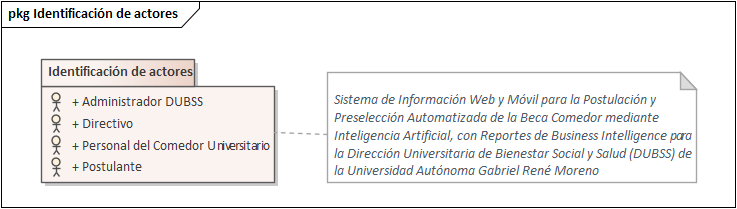
\includegraphics[width=\textwidth,height=0.85\textheight,keepaspectratio]{images/029_Identificacion_de_Actores.png}

\smallskip
\noindent\raggedright\textit{Nota.} Elaboración propia.
\end{figure}

A continuación, se describe el rol de cada actor identificado en la Figura~\ref{fig:identificacion_actores}:

\begin{itemize}
    \item \textbf{Postulante:} estudiante de la UAGRM encargado de registrarse en el sistema, completar el formulario socioeconómico, digitalizar y adjuntar su documentación, enviar su postulación a la Beca Comedor y consultar su estado. Una vez adjudicado, consulta su historial de asistencia y el estado de su beca.
    \item \textbf{Administrador DUBSS:} usuario de la Dirección Universitaria de Bienestar Social y Salud con acceso a las funcionalidades de gestión del sistema. Gestiona las convocatorias, los usuarios y roles, audita los expedientes de los finalistas, devuelve, archiva o adjudica postulaciones, publica los resultados, administra el padrón de becados, genera las planillas de asistencia, consulta la bitácora y parametriza el modelo de preselección.
    \item \textbf{Directivo:} usuario encargado de la toma de decisiones institucionales que consulta el dashboard de indicadores de Business Intelligence sobre postulaciones, adjudicaciones y asistencia.
    \item \textbf{Personal del Comedor Universitario:} usuario encargado de registrar diariamente la asistencia digital de los estudiantes becados que acuden al comedor.
\end{itemize}

La Figura~\ref{fig:descripcion_actores} resume el rol de cada actor mediante un diagrama de actores con su descripción.

\begin{figure}[H]
\caption{Descripción de actores}
\label{fig:descripcion_actores}
\centering
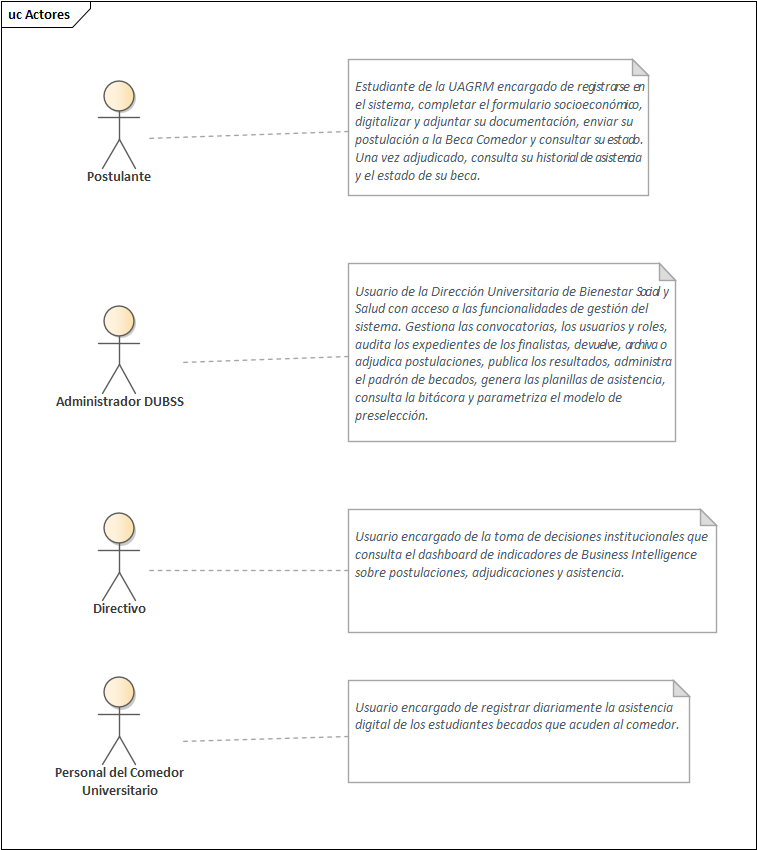
\includegraphics[width=\textwidth,height=0.85\textheight,keepaspectratio]{images/030_Descripcion_de_Actores.png}

\smallskip
\noindent\raggedright\textit{Nota.} Elaboración propia.
\end{figure}

% ------------------------------------------------------------------------------
% 5.2. IDENTIFICACIÓN DE CASOS DE USO
% ------------------------------------------------------------------------------
\wfa{\wn{5.2}. Identificación de Casos de Uso}\label{sec:cap5_identificacion_cu}

A partir de los actores identificados en la Sección~\wn{5.1} y de los requisitos funcionales especificados en \wfref{4}, se identificaron veintiséis casos de uso que cubren el ciclo completo de la Beca Comedor. La Tabla~\ref{tab:identificacion_cu} presenta cada caso de uso con su actor principal y el requisito funcional que lo respalda.

\refstepcounter{table}\label{tab:identificacion_cu}
\addcontentsline{lot}{table}{\protect\numberline{\thetable}Identificación de casos de uso del sistema}
\noindent\textbf{Tabla~\thetable}\par\nopagebreak
\noindent\textit{Identificación de casos de uso del sistema}\par\nopagebreak
\begin{longtable}{>{\raggedright\arraybackslash}p{1.4cm} >{\raggedright\arraybackslash}p{6.4cm} >{\raggedright\arraybackslash}p{3.2cm} >{\raggedright\arraybackslash}p{1.5cm}}
\toprule
ID & Caso de uso & Actor principal & RF \\
\midrule
\endfirsthead
\toprule
ID & Caso de uso & Actor principal & RF \\
\midrule
\endhead
\midrule
\multicolumn{4}{r}{\textit{Continúa en la siguiente página}} \
\endfoot
\bottomrule
\multicolumn{4}{l}{\textit{Nota.} Elaboración propia.} \
\endlastfoot
CU-01 & Registrarse y autenticarse & Usuario del Sistema & RF-01 \\
CU-02 & Enviar postulación a Beca Comedor & Postulante & RF-02 \\
CU-03 & Precalificar postulación con Inteligencia Artificial & Sistema (Módulo IA) & RF-03 \\
CU-04 & Consultar estado de postulación & Postulante & RF-06 \\
CU-05 & Auditar y adjudicar becas & Administrador DUBSS & RF-04 \\
CU-06 & Visualizar lista priorizada de postulantes & Administrador DUBSS & RF-04 \\
CU-07 & Auditar expediente finalista & Administrador DUBSS & RF-04 \\
CU-08 & Generar acta de adjudicación & Administrador DUBSS & RF-04 \\
CU-09 & Generar planilla de asistencia & Administrador DUBSS & RF-05 \\
CU-10 & Registrar asistencia digital & Personal del Comedor & RF-05 \\
CU-11 & Cotejar registro contra respaldo físico & Administrador DUBSS & RF-05 \\
CU-12 & Visualizar dashboard de indicadores BI & Directivo & RF-07 \\
CU-13 & Gestionar convocatoria y gestión académica & Administrador DUBSS & RF-08 \\
CU-14 & Gestionar usuarios y roles & Administrador DUBSS & RF-09 \\
CU-15 & Recuperar contraseña / gestionar perfil & Usuario del Sistema & RF-10 \\
CU-16 & Digitalizar y adjuntar documentos & Postulante & RF-11 \\
CU-17 & Guardar borrador de postulación & Postulante & RF-12 \\
CU-18 & Validar elegibilidad y duplicados & Sistema (Módulo IA) & RF-13 \\
CU-19 & Devolver postulación para corrección & Administrador DUBSS & RF-14 \\
CU-20 & Archivar o rechazar postulación & Administrador DUBSS & RF-15 \\
CU-21 & Notificar finalistas, registrar entrega de documentación física y publicar comunicados/avisos & Administrador DUBSS & RF-16 \\
CU-22 & Publicar resultados de adjudicación & Administrador DUBSS & RF-17 \\
CU-23 & Gestionar padrón de becados (baja, suspensión, reemplazo) & Administrador DUBSS & RF-18 \\
CU-24 & Consultar historial de asistencia y estado de beca & Postulante (becado) & RF-19 \\
CU-25 & Consultar bitácora de acciones & Administrador DUBSS & RF-20 \\
CU-26 & Parametrizar modelo de preselección y reprocesar puntajes & Administrador DUBSS & RF-21 \\
\end{longtable}
\addtocounter{table}{-1}

% ------------------------------------------------------------------------------
% 5.3. PRIORIZACIÓN DE CASOS DE USO
% ------------------------------------------------------------------------------
\wfa{\wn{5.3}. Priorización de Casos de Uso}\label{sec:cap5_priorizacion_cu}

La priorización de los casos de uso se realizó según su aporte al objetivo del proyecto y sus dependencias, y se clasificó en tres niveles:

\begin{itemize}
    \item \textbf{Alta:} caso de uso indispensable; sin él el sistema no cumple su función.
    \item \textbf{Media:} caso de uso necesario para que el sistema opere de forma completa.
    \item \textbf{Baja:} caso de uso complementario, cuya ausencia no bloquea el flujo principal.
\end{itemize}

Además, dentro de cada nivel se definió un orden de implementación sugerido que respeta las dependencias entre casos de uso, indicadas en la columna «Depende de». Del total de veintiséis casos de uso, dieciséis tienen prioridad alta, siete media y tres baja. Las Tablas~\ref{tab:prioridad_alta}, \ref{tab:prioridad_media} y~\ref{tab:prioridad_baja} presentan los casos de uso de cada nivel.

\refstepcounter{table}\label{tab:prioridad_alta}
\addcontentsline{lot}{table}{\protect\numberline{\thetable}Casos de uso de prioridad alta}
\noindent\textbf{Tabla~\thetable}\par\nopagebreak
\noindent\textit{Casos de uso de prioridad alta}\par\nopagebreak
\begin{longtable}{>{\raggedright\arraybackslash}p{1.2cm} >{\raggedright\arraybackslash}p{1.4cm} >{\raggedright\arraybackslash}p{4.4cm} >{\raggedright\arraybackslash}p{1.9cm} >{\raggedright\arraybackslash}p{3.8cm}}
\toprule
Orden & ID & Caso de uso & Depende de & Justificación \\
\midrule
\endfirsthead
\toprule
Orden & ID & Caso de uso & Depende de & Justificación \\
\midrule
\endhead
\midrule
\multicolumn{5}{r}{\textit{Continúa en la siguiente página}} \\
\endfoot
\bottomrule
\multicolumn{5}{l}{\textit{Nota.} Elaboración propia.} \\
\endlastfoot
1 & CU-01 & Registrarse y autenticarse & --- & Base de seguridad y roles de todo el sistema. \\
2 & CU-14 & Gestionar usuarios y roles & CU-01 & Habilita las cuentas del personal de la DUBSS. \\
3 & CU-13 & Gestionar convocatoria y gestión académica & CU-14 & Sin convocatoria abierta no hay postulaciones. \\
4 & CU-16 & Digitalizar y adjuntar documentos & CU-01 & Parte esencial de la postulación. \\
5 & CU-18 & Validar elegibilidad y duplicados & CU-13 & Garantiza la integridad de las postulaciones. \\
6 & CU-02 & Enviar postulación a Beca Comedor & CU-13, CU-16, CU-18 & Entrada principal de datos del sistema. \\
7 & CU-03 & Precalificar postulación con Inteligencia Artificial & CU-02 & Núcleo diferenciador del proyecto. \\
8 & CU-04 & Consultar estado de postulación & CU-02 & Transparencia para el postulante. \\
9 & CU-06 & Visualizar lista priorizada de postulantes & CU-03 & Resuelve la revisión al azar de expedientes. \\
10 & CU-05 & Auditar y adjudicar becas & CU-06 & Decisión final del proceso. \\
11 & CU-07 & Auditar expediente finalista & CU-06 & Validación física de los finalistas. \\
12 & CU-19 & Devolver postulación para corrección & CU-07 & Evita descartar expedientes subsanables. \\
13 & CU-20 & Archivar o rechazar postulación & CU-07 & Cierra formalmente los expedientes. \\
14 & CU-21 & Notificar finalistas y registrar entrega de documentación física & CU-07 & Coordina la auditoría física. \\
15 & CU-22 & Publicar resultados de adjudicación & CU-05 & Cierra el proceso de selección. \\
16 & CU-12 & Visualizar dashboard de indicadores BI & CU-02, CU-05, CU-10 & Objetivo del proyecto; requiere datos acumulados. \\
\end{longtable}
\addtocounter{table}{-1}

\refstepcounter{table}\label{tab:prioridad_media}
\addcontentsline{lot}{table}{\protect\numberline{\thetable}Casos de uso de prioridad media}
\noindent\textbf{Tabla~\thetable}\par\nopagebreak
\noindent\textit{Casos de uso de prioridad media}\par\nopagebreak
\begin{longtable}{>{\raggedright\arraybackslash}p{1.2cm} >{\raggedright\arraybackslash}p{1.4cm} >{\raggedright\arraybackslash}p{4.4cm} >{\raggedright\arraybackslash}p{1.9cm} >{\raggedright\arraybackslash}p{3.8cm}}
\toprule
Orden & ID & Caso de uso & Depende de & Justificación \\
\midrule
\endfirsthead
\toprule
Orden & ID & Caso de uso & Depende de & Justificación \\
\midrule
\endhead
\midrule
\multicolumn{5}{r}{\textit{Continúa en la siguiente página}} \\
\endfoot
\bottomrule
\multicolumn{5}{l}{\textit{Nota.} Elaboración propia.} \\
\endlastfoot
1 & CU-23 & Gestionar padrón de becados & CU-05 & Base del control de asistencia. \\
2 & CU-09 & Generar planilla de asistencia & CU-23 & Exigida por las auditorías externas. \\
3 & CU-10 & Registrar asistencia digital & CU-23 & Registra la asistencia diaria de los becados. \\
4 & CU-24 & Consultar historial de asistencia y estado de beca & CU-10 & Vista de seguimiento para el becado. \\
5 & CU-08 & Generar acta de adjudicación & CU-05 & Formaliza el resultado de la adjudicación. \\
6 & CU-11 & Cotejar registro contra respaldo físico & CU-10 & Contrasta el registro digital con las planillas físicas. \\
7 & CU-25 & Consultar bitácora de acciones & CU-01 & Trazabilidad transversal del sistema. \\
\end{longtable}
\addtocounter{table}{-1}

\refstepcounter{table}\label{tab:prioridad_baja}
\addcontentsline{lot}{table}{\protect\numberline{\thetable}Casos de uso de prioridad baja}
\noindent\textbf{Tabla~\thetable}\par\nopagebreak
\noindent\textit{Casos de uso de prioridad baja}\par\nopagebreak
\begin{longtable}{>{\raggedright\arraybackslash}p{1.2cm} >{\raggedright\arraybackslash}p{1.4cm} >{\raggedright\arraybackslash}p{4.4cm} >{\raggedright\arraybackslash}p{1.9cm} >{\raggedright\arraybackslash}p{3.8cm}}
\toprule
Orden & ID & Caso de uso & Depende de & Justificación \\
\midrule
\endfirsthead
\toprule
Orden & ID & Caso de uso & Depende de & Justificación \\
\midrule
\endhead
\midrule
\multicolumn{5}{r}{\textit{Continúa en la siguiente página}} \\
\endfoot
\bottomrule
\multicolumn{5}{l}{\textit{Nota.} Elaboración propia.} \\
\endlastfoot
1 & CU-15 & Recuperar contraseña / gestionar perfil & CU-01 & Comodidad; no bloquea el flujo principal. \\
2 & CU-17 & Guardar borrador de postulación & CU-02 & Facilita completar la postulación en varias sesiones. \\
3 & CU-26 & Parametrizar modelo de preselección y reprocesar puntajes & CU-03 & Ajuste fino posterior al modelo. \\
\end{longtable}
\addtocounter{table}{-1}

% ------------------------------------------------------------------------------
% 5.4. DETALLE DE CASOS DE USO
% Cada CU: (1) diagrama de contexto [pendiente de insertar] y (2) tabla de detalle.
% ------------------------------------------------------------------------------
% Listas compactas para las celdas de las tablas de detalle.
\newenvironment{cupasos}{\begin{enumerate}\setlength{\itemsep}{1pt}\setlength{\topsep}{2pt}\setlength{\parsep}{0pt}\setlength{\parskip}{0pt}\setlength{\leftmargin}{1.5em}}{\end{enumerate}}
\newenvironment{cuvin}{\begin{itemize}\setlength{\itemsep}{1pt}\setlength{\topsep}{2pt}\setlength{\parsep}{0pt}\setlength{\parskip}{0pt}\setlength{\leftmargin}{1.2em}}{\end{itemize}}

\subsection{5.4. Detalle de Casos de Uso}\label{sec:cap5_detalle_cu}

\subsubsection{5.4.1. CU-01 Registrarse y autenticarse}\label{sec:cap5_cu01}

\begin{figure}[H]
\caption{Diagrama de contexto del CU-01}
\label{fig:ctx_cu01}
\centering
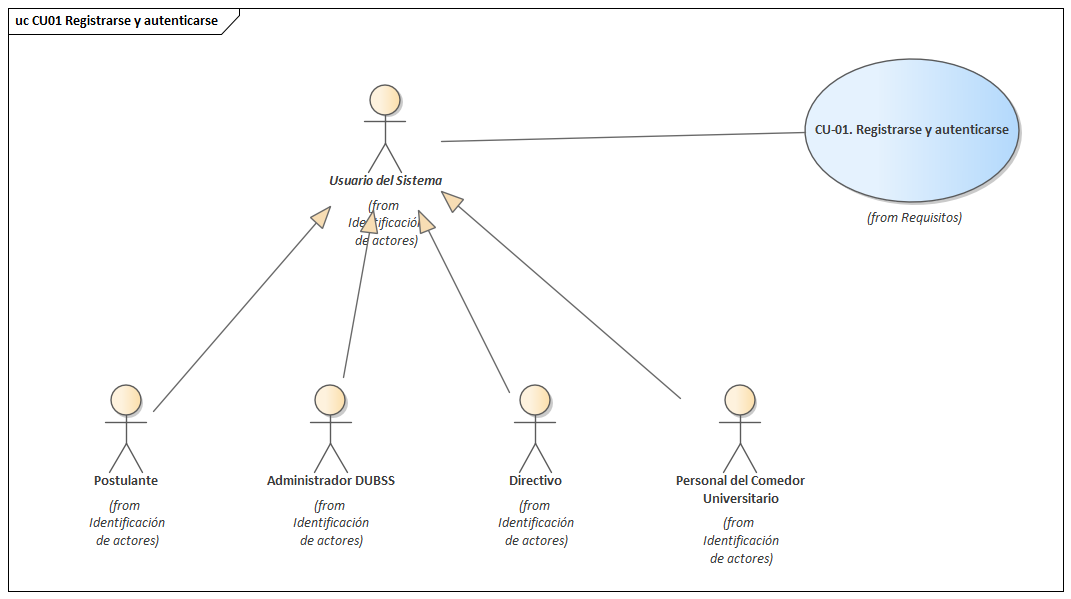
\includegraphics[width=0.8\textwidth,height=0.4\textheight,keepaspectratio]{images/038_CU01_Registrarse_Autenticarse.png}

\smallskip
\noindent\raggedright\textit{Nota.} Elaboración propia.
\end{figure}

\refstepcounter{table}\label{tab:detalle_cu01}
\addcontentsline{lot}{table}{\protect\numberline{\thetable}Detalle del CU-01: Registrarse y autenticarse}
\noindent\textbf{Tabla~\thetable}\par\nopagebreak
\noindent\textit{Detalle del CU-01: Registrarse y autenticarse}\par\nopagebreak
\begingroup\small\linespread{1}\selectfont
\begin{longtable}{>{\raggedright\arraybackslash}p{2.9cm} >{\raggedright\arraybackslash}p{12.6cm}}
\toprule
\textbf{Caso de Uso} & \textbf{CU-01. Registrarse y autenticarse} \\
\midrule
\endfirsthead
\toprule
\textbf{Caso de Uso} & \textbf{CU-01. Registrarse y autenticarse} \\
\midrule
\endhead
\endfoot
\bottomrule
\multicolumn{2}{l}{\textit{Nota.} Elaboración propia.} \\
\endlastfoot
\textbf{Propósito} & Permitir que el Postulante cree su cuenta y que cualquier usuario del sistema inicie y cierre sesión para acceder, de forma segura, solo a las funcionalidades correspondientes a su rol, desde el portal web o la aplicación móvil. \\
\midrule
\textbf{Descripción} & Este caso de uso describe tres flujos: el registro de un Postulante, el inicio de sesión de cualquier usuario del sistema (Postulante, Administrador DUBSS, Directivo o Personal del Comedor Universitario) con su correo electrónico y contraseña, y el cierre de sesión. La autenticación la resuelve el propio sistema (RF-01): el backend guarda la contraseña únicamente como hash, verifica las credenciales, emite un token de acceso de vida corta y un token de renovación por dispositivo, y comprueba el token de acceso en cada petición. Una vez autenticado, el sistema identifica el rol del usuario y lo redirige al módulo que le corresponde. Las cuentas del personal (Administrador DUBSS, Directivo y Personal del Comedor) no se autorregistran: son creadas por el Administrador DUBSS en el CU-14. El cierre de sesión se documenta dentro de este caso de uso y no constituye un caso de uso independiente. El CU-15 extiende este caso de uso para la recuperación de contraseña. Respalda el RF-01. \\
\midrule
\textbf{Actores} & Usuario del Sistema (actor abstracto generalizado por Postulante, Administrador DUBSS, Directivo y Personal del Comedor Universitario). \\
\midrule
\textbf{Actor Iniciador} & Usuario del Sistema. \\
\midrule
\textbf{Precondición} & \vspace{-\baselineskip}\begin{cuvin}
    \item El usuario dispone de acceso al portal web o a la aplicación móvil y de conexión a Internet.
    \item Para el registro: no existe una cuenta asociada al CI, al registro universitario ni al correo electrónico del postulante.
    \item Para el inicio de sesión: el usuario cuenta con una cuenta registrada y activa (creada por autorregistro si es Postulante, o por el Administrador DUBSS en el CU-14 si es personal).
    \item Para el cierre de sesión: el usuario tiene una sesión abierta.
\end{cuvin} \\
\midrule
\textbf{Proceso} & \textbf{Flujo principal A: registro de un Postulante.}
\begin{cupasos}
    \item El usuario selecciona la opción «Crear cuenta» en la pantalla de acceso.
    \item El sistema muestra el formulario de registro (nombres, apellidos, CI, registro universitario, carrera, teléfono, correo electrónico, contraseña y confirmación de contraseña).
    \item El usuario completa los datos y confirma el registro.
    \item El sistema valida que los campos obligatorios estén completos, que su formato sea correcto (el registro universitario tiene 9 dígitos numéricos y no empieza por 0), que la contraseña cumpla la política (al menos 6 caracteres, sin obligación de mayúsculas, números ni símbolos) y coincida con su confirmación, y que el CI, el registro universitario y el correo electrónico no existan en el sistema.
    \item El sistema registra en la base de datos al usuario con el rol Postulante y activo, guardando la contraseña únicamente como hash, junto con su perfil de postulante, y anota el registro en la bitácora.
    \item El sistema informa que el registro fue exitoso, inicia la sesión del usuario y lo redirige al módulo del Postulante.
\end{cupasos} \\
 & \textbf{Flujo principal B: inicio de sesión.}
\begin{cupasos}
    \item El usuario accede a la pantalla de inicio de sesión del portal web o de la aplicación móvil.
    \item El usuario ingresa su correo electrónico y su contraseña.
    \item El sistema verifica las credenciales comparando la contraseña ingresada con el hash almacenado.
    \item El sistema comprueba que la cuenta esté activa y no bloqueada, y obtiene el rol del usuario.
    \item El sistema abre la sesión (emite el token de acceso y el token de renovación del dispositivo) y registra el acceso en la bitácora.
    \item El sistema redirige al usuario según su rol: el Postulante a su módulo de postulación, el Administrador DUBSS al panel de gestión, el Directivo al dashboard de indicadores y el Personal del Comedor al registro de asistencia.
\end{cupasos} \\
 & \textbf{Flujo principal C: cierre de sesión.}
\begin{cupasos}
    \item El usuario selecciona la opción «Cerrar sesión» en el menú de su cuenta.
    \item El sistema revoca la sesión del usuario en ese dispositivo y deja de reconocerla.
    \item El sistema redirige al usuario a la pantalla de acceso.
\end{cupasos} \\
 & \textbf{Flujos alternativos.}
\begin{cuvin}
    \item A1 (flujo A, paso 4): si el CI, el registro universitario o el correo electrónico ya están registrados, el sistema rechaza el registro, indica el campo en conflicto y no crea la cuenta.
    \item A2 (flujo A, paso 4): si faltan campos obligatorios, el formato es inválido, la contraseña no cumple la política o no coincide con su confirmación, el sistema marca los campos con error y permite corregirlos, sin crear la cuenta.
    \item A3 (flujo B, paso 3): si el correo no existe o la contraseña es incorrecta, el sistema muestra el mismo mensaje de error en ambos casos (sin revelar cuál dato falló) y permite reintentar.
    \item A4 (flujo B, paso 4): si la cuenta está desactivada, el sistema niega el acceso, indica que debe comunicarse con la DUBSS y no abre sesión.
    \item A5 (flujo B, paso 2): si el usuario selecciona «¿Olvidó su contraseña?», se ejecuta el CU-15.
    \item A6 (flujo B, paso 3): tras varios intentos fallidos consecutivos, el sistema bloquea temporalmente el acceso de esa cuenta y lo niega aunque la contraseña sea correcta. El sistema bloquea a los 5 intentos, por 5 minutos la primera vez y por un lapso mayor si el usuario continúa fallando (hoy: 5 minutos, 15 minutos, 1 hora y 24 horas); la escala exacta está por definir con la DUBSS. Un inicio de sesión correcto reinicia el contador.
    \item A7 (flujo A, paso 4): si la petición de registro llega repetida (doble envío o reintento), el sistema la procesa de forma idempotente y no crea dos cuentas.
    \item A8 (flujo B, pasos 5 y 6): si el token de acceso venció, el sistema lo renueva automáticamente con el token de renovación del dispositivo, que se reemplaza por uno nuevo en cada uso; si la sesión ya no es válida (expiró o fue revocada), el sistema redirige al usuario a la pantalla de inicio de sesión.
    \item A9 (cualquier paso): si falla la conexión con el servidor o con un servicio del que depende, el sistema informa el error con un mensaje claro, no crea ni modifica datos y permite reintentar.
    \item A10 (flujo C, paso 2): si la sesión ya había expirado o se había cerrado antes de solicitar el cierre, el sistema igualmente redirige al usuario a la pantalla de acceso, sin mostrar error.
\end{cuvin} \\
\midrule
\textbf{Postcondición} & \vspace{-\baselineskip}\begin{cuvin}
    \item Registro: la cuenta del Postulante queda creada, activa y con el rol Postulante, y el usuario tiene una sesión abierta.
    \item Inicio de sesión: el usuario tiene una sesión activa con los permisos de su rol, se encuentra en el módulo que le corresponde y su acceso queda registrado en la bitácora (consultable en el CU-25).
    \item Cierre de sesión: el dispositivo ya no tiene sesión abierta y cualquier pantalla privada lleva a la pantalla de acceso; las sesiones en otros dispositivos no se ven afectadas.
\end{cuvin} \\
\midrule
\textbf{Excepciones} & \vspace{-\baselineskip}\begin{cuvin}
    \item Credenciales inválidas o cuenta inexistente.
    \item Cuenta desactivada o bloqueada temporalmente.
    \item Sesión inválida o expirada.
    \item Error de conexión con el servidor o con la base de datos.
    \item Petición de registro duplicada (se procesa de forma idempotente, sin crear dos cuentas).
\end{cuvin} \\
\end{longtable}
\endgroup
\addtocounter{table}{-1}

\subsubsection{5.4.2. CU-02 Enviar postulación a Beca Comedor}\label{sec:cap5_cu02}

\begin{figure}[H]
\caption{Diagrama de contexto del CU-02}
\label{fig:ctx_cu02}
\centering
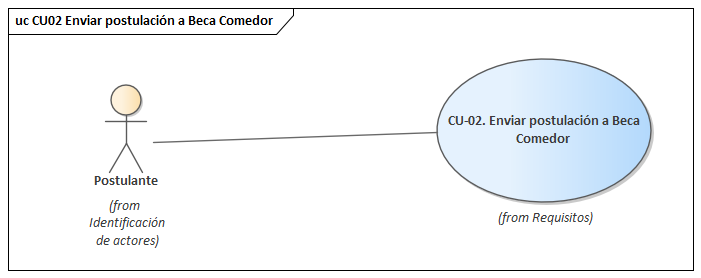
\includegraphics[width=0.8\textwidth,height=0.4\textheight,keepaspectratio]{images/039_CU02_Enviar_Postulacion_Beca_Comedor.png}

\smallskip
\noindent\raggedright\textit{Nota.} Elaboración propia.
\end{figure}

\refstepcounter{table}\label{tab:detalle_cu02}
\addcontentsline{lot}{table}{\protect\numberline{\thetable}Detalle del CU-02: Enviar postulación a Beca Comedor}
\noindent\textbf{Tabla~\thetable}\par\nopagebreak
\noindent\textit{Detalle del CU-02: Enviar postulación a Beca Comedor}\par\nopagebreak
\begingroup\small\linespread{1}\selectfont
\begin{longtable}{>{\raggedright\arraybackslash}p{2.9cm} >{\raggedright\arraybackslash}p{12.6cm}}
\toprule
\textbf{Caso de Uso} & \textbf{CU-02. Enviar postulación a Beca Comedor} \\
\midrule
\endfirsthead
\toprule
\textbf{Caso de Uso} & \textbf{CU-02. Enviar postulación a Beca Comedor} \\
\midrule
\endhead
\endfoot
\bottomrule
\multicolumn{2}{l}{\textit{Nota.} Elaboración propia.} \\
\endlastfoot
\textbf{Propósito} & Permitir al Postulante completar el formulario socioeconómico, adjuntar su documentación digitalizada y enviar formalmente su postulación a la Beca Comedor de la convocatoria vigente. \\
\midrule
\textbf{Descripción} & Este caso de uso describe cómo el Postulante registra su postulación desde el portal web o la aplicación móvil. Incluye la digitalización y carga de documentos (CU-16), la validación de elegibilidad y duplicados (CU-18) y la precalificación automática con Inteligencia Artificial (CU-03). El CU-17 lo extiende para guardar la postulación como borrador. Respalda el RF-02. \\
\midrule
\textbf{Actores} & Postulante. \\
\midrule
\textbf{Actor Iniciador} & Postulante. \\
\midrule
\textbf{Precondición} & \vspace{-\baselineskip}\begin{cuvin}
    \item El Postulante está autenticado en el sistema (CU-01).
    \item Existe una convocatoria abierta (CU-13) para la gestión académica vigente.
    \item El Postulante no tiene otra postulación vigente en la misma gestión, salvo que la suya haya sido devuelta para corrección (CU-19).
    \item El Postulante dispone de los documentos obligatorios definidos en la convocatoria.
\end{cuvin} \\
\midrule
\textbf{Proceso} & \textbf{Flujo principal.}
\begin{cupasos}
    \item El Postulante selecciona la opción «Nueva postulación».
    \item El sistema verifica que exista una convocatoria abierta y muestra el formulario socioeconómico con los datos del perfil precargados (nombre, CI y carrera).
    \item El Postulante completa las variables socioeconómicas: ingresos familiares, número de dependientes, procedencia, patrimonio, estado de vulnerabilidad y promedio académico.
    \item El Postulante digitaliza o adjunta los documentos de respaldo requeridos (se incluye el CU-16).
    \item El Postulante selecciona «Enviar postulación».
    \item El sistema verifica que no falte ningún campo ni documento obligatorio y que los datos tengan un formato válido.
    \item El sistema valida la elegibilidad del Postulante y la inexistencia de duplicados (se incluye el CU-18).
    \item El sistema registra la postulación con estado «pendiente», asociándola a la convocatoria y gestión académica vigentes, con su fecha y hora de envío.
    \item El sistema solicita la precalificación de la postulación (se incluye el CU-03).
    \item El sistema confirma la recepción de la postulación y muestra al Postulante un comprobante con su código de postulación.
\end{cupasos} \\
 & \textbf{Flujos alternativos.}
\begin{cuvin}
    \item A1 (paso 1): si no existe una convocatoria abierta, el sistema impide iniciar la postulación e informa las fechas de la próxima convocatoria, si están definidas.
    \item A2 (pasos 3 y 4): si el Postulante desea continuar más tarde, puede guardar su avance como borrador (CU-17).
    \item A3 (paso 6): si faltan campos o documentos obligatorios, el sistema resalta lo faltante y no permite enviar la postulación.
    \item A4 (paso 7): si el Postulante no es elegible o ya tiene una postulación vigente en la gestión, el sistema rechaza el envío e informa el motivo.
    \item A5 (paso 1): si el Postulante tiene una postulación en estado «devuelta», el sistema le permite abrirla, corregirla y reenviarla; esta no se considera duplicada y se conserva el historial de devoluciones y reenvíos.
    \item A6 (paso 5): si el Postulante presiona repetidamente el botón de envío o la petición llega duplicada, el sistema la procesa una sola vez (idempotencia).
    \item A7 (paso 9): si el módulo de IA no responde, la postulación queda registrada con estado «pendiente» y la precalificación se reintenta automáticamente; el Postulante no pierde su envío.
    \item A8 (pasos 2 a 5): si la convocatoria se cierra mientras el Postulante completa el formulario, el sistema no acepta el envío e informa que el plazo finalizó.
\end{cuvin} \\
\midrule
\textbf{Postcondición} & \vspace{-\baselineskip}\begin{cuvin}
    \item La postulación queda almacenada con estado «pendiente» (o «calificada» una vez ejecutado el CU-03), asociada al Postulante, a la convocatoria y a la gestión académica.
    \item Los documentos adjuntos quedan almacenados en MinIO y vinculados a la postulación.
    \item El Postulante puede consultar el estado de su postulación (CU-04).
\end{cuvin} \\
\midrule
\textbf{Excepciones} & \vspace{-\baselineskip}\begin{cuvin}
    \item Autenticación inválida o sesión expirada.
    \item Falta de permisos suficientes (el usuario no tiene el rol Postulante).
    \item Datos ingresados no válidos o campos obligatorios incompletos.
    \item Convocatoria cerrada o inexistente.
    \item Postulación duplicada o Postulante no elegible.
    \item Error al almacenar los archivos en MinIO.
    \item Error de conexión con el servidor o la base de datos durante el envío.
\end{cuvin} \\
\end{longtable}
\endgroup
\addtocounter{table}{-1}

\subsubsection{5.4.3. CU-03 Precalificar postulación con Inteligencia Artificial}\label{sec:cap5_cu03}

\begin{figure}[H]
\caption{Diagrama de contexto del CU-03}
\label{fig:ctx_cu03}
\centering
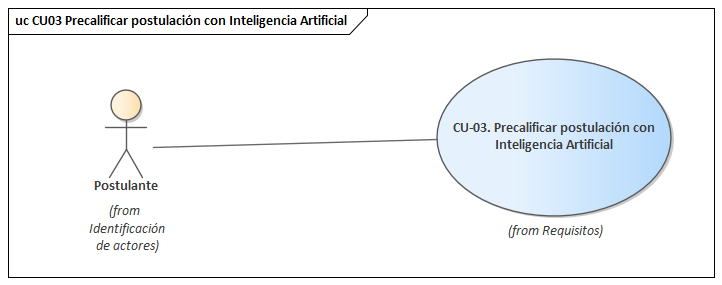
\includegraphics[width=0.8\textwidth,height=0.4\textheight,keepaspectratio]{images/040_CU03_Precalificar_Postulacion_IA.png}

\smallskip
\noindent\raggedright\textit{Nota.} Elaboración propia.
\end{figure}

\refstepcounter{table}\label{tab:detalle_cu03}
\addcontentsline{lot}{table}{\protect\numberline{\thetable}Detalle del CU-03: Precalificar postulación con Inteligencia Artificial}
\noindent\textbf{Tabla~\thetable}\par\nopagebreak
\noindent\textit{Detalle del CU-03: Precalificar postulación con Inteligencia Artificial}\par\nopagebreak
\begingroup\small\linespread{1}\selectfont
\begin{longtable}{>{\raggedright\arraybackslash}p{2.9cm} >{\raggedright\arraybackslash}p{12.6cm}}
\toprule
\textbf{Caso de Uso} & \textbf{CU-03. Precalificar postulación con Inteligencia Artificial} \\
\midrule
\endfirsthead
\toprule
\textbf{Caso de Uso} & \textbf{CU-03. Precalificar postulación con Inteligencia Artificial} \\
\midrule
\endhead
\endfoot
\bottomrule
\multicolumn{2}{l}{\textit{Nota.} Elaboración propia.} \\
\endlastfoot
\textbf{Propósito} & Calcular automáticamente, mediante un modelo de Inteligencia Artificial, el puntaje de vulnerabilidad de cada postulación recibida, para ordenar objetivamente a los postulantes según su nivel de necesidad. \\
\midrule
\textbf{Descripción} & Este caso de uso describe cómo el sistema precalifica cada postulación enviada, enviando sus variables socioeconómicas y académicas al módulo de IA (desarrollado en Python y consumido mediante API) y registrando el puntaje obtenido junto con su fecha de cálculo. El puntaje permite construir la lista priorizada que usa el Administrador DUBSS para auditar únicamente a los finalistas (CU-06). Es incluido por el CU-02 y extendido por el CU-26, que permite reprocesar los puntajes. Respalda el RF-03. \\
\midrule
\textbf{Actores} & Postulante. \\
\midrule
\textbf{Actor Iniciador} & Postulante (a través del CU-02, al enviar su postulación; el sistema ejecuta la precalificación mediante el módulo de IA). \\
\midrule
\textbf{Precondición} & \vspace{-\baselineskip}\begin{cuvin}
    \item La postulación fue enviada, superó la validación de elegibilidad y duplicados (CU-18) y se encuentra en estado «pendiente».
    \item El módulo de IA está disponible y tiene cargados los parámetros vigentes del modelo (criterios y ponderaciones por definir con la DUBSS).
    \item La postulación contiene las variables requeridas por el modelo: ingresos familiares, dependientes, procedencia, carrera, patrimonio, estado de vulnerabilidad y promedio académico.
\end{cuvin} \\
\midrule
\textbf{Proceso} & \textbf{Flujo principal.}
\begin{cupasos}
    \item El sistema (backend) detecta una postulación pendiente de precalificar y prepara el conjunto de variables socioeconómicas y académicas declaradas.
    \item El sistema envía la solicitud de cálculo al módulo de IA mediante la API.
    \item El módulo de IA valida que los datos recibidos estén completos y sean consistentes.
    \item El módulo de IA aplica el modelo con los parámetros vigentes y calcula el puntaje de vulnerabilidad.
    \item El módulo de IA devuelve el puntaje al sistema.
    \item El sistema registra el puntaje junto con la fecha y hora de cálculo y la versión de los parámetros utilizados, conservando los puntajes anteriores si existieran.
    \item El sistema actualiza el estado de la postulación a «calificada» e incorpora la postulación a la lista priorizada.
\end{cupasos} \\
 & \textbf{Flujos alternativos.}
\begin{cuvin}
    \item A1 (paso 3): si los datos están incompletos o son inconsistentes, el módulo de IA no calcula el puntaje; el sistema registra el error y deja la postulación marcada para revisión.
    \item A2 (paso 2): si el módulo de IA no está disponible o excede el tiempo de espera, el sistema registra el fallo, mantiene la postulación en estado «pendiente» y reintenta el cálculo automáticamente.
    \item A3 (paso 1): si la solicitud proviene del reprocesamiento (CU-26), el sistema calcula un nuevo puntaje con los parámetros actualizados y conserva el puntaje anterior para trazabilidad.
    \item A4 (paso 1): si se recibe una solicitud duplicada para la misma postulación y la misma versión de parámetros, el sistema no genera un segundo puntaje (idempotencia).
    \item A5 (paso 1): ante picos de envíos (por ejemplo, al cierre de la convocatoria), el sistema encola las solicitudes y las procesa en orden, de modo que la totalidad de las postulaciones (hasta 20,000 por gestión) sea procesada sin intervención manual.
\end{cuvin} \\
\midrule
\textbf{Postcondición} & \vspace{-\baselineskip}\begin{cuvin}
    \item Cada postulación procesada tiene un puntaje de vulnerabilidad registrado con su fecha de cálculo, lo que permite su trazabilidad.
    \item La postulación queda en estado «calificada» y disponible en la lista priorizada (CU-06).
\end{cuvin} \\
\midrule
\textbf{Excepciones} & \vspace{-\baselineskip}\begin{cuvin}
    \item Módulo de IA no disponible o tiempo de espera agotado (el cálculo individual debe completarse en un máximo de 5 segundos en condiciones normales).
    \item Datos de la postulación incompletos o inconsistentes.
    \item Error en la comunicación entre el backend y el módulo de IA.
    \item Error de conexión con la base de datos al registrar el puntaje.
\end{cuvin} \\
\end{longtable}
\endgroup
\addtocounter{table}{-1}

\subsubsection{5.4.4. CU-04 Consultar estado de postulación}\label{sec:cap5_cu04}

\begin{figure}[H]
\caption{Diagrama de contexto del CU-04}
\label{fig:ctx_cu04}
\centering
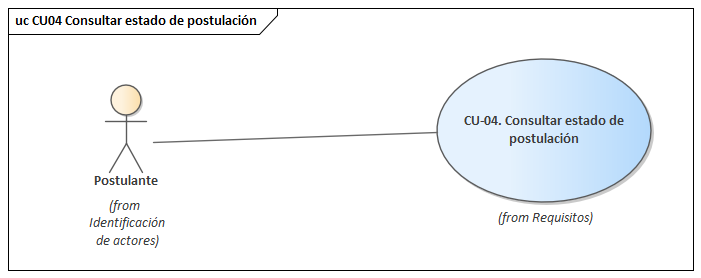
\includegraphics[width=0.8\textwidth,height=0.4\textheight,keepaspectratio]{images/041_CU04_Consultar_Estado_Postulacion.png}

\smallskip
\noindent\raggedright\textit{Nota.} Elaboración propia.
\end{figure}

\refstepcounter{table}\label{tab:detalle_cu04}
\addcontentsline{lot}{table}{\protect\numberline{\thetable}Detalle del CU-04: Consultar estado de postulación}
\noindent\textbf{Tabla~\thetable}\par\nopagebreak
\noindent\textit{Detalle del CU-04: Consultar estado de postulación}\par\nopagebreak
\begingroup\small\linespread{1}\selectfont
\begin{longtable}{>{\raggedright\arraybackslash}p{2.9cm} >{\raggedright\arraybackslash}p{12.6cm}}
\toprule
\textbf{Caso de Uso} & \textbf{CU-04. Consultar estado de postulación} \\
\midrule
\endfirsthead
\toprule
\textbf{Caso de Uso} & \textbf{CU-04. Consultar estado de postulación} \\
\midrule
\endhead
\endfoot
\bottomrule
\multicolumn{2}{l}{\textit{Nota.} Elaboración propia.} \\
\endlastfoot
\textbf{Propósito} & Permitir al Postulante realizar el seguimiento del estado de su postulación sin necesidad de acudir presencialmente a la DUBSS. \\
\midrule
\textbf{Descripción} & Este caso de uso describe cómo el Postulante consulta, desde el portal web o la aplicación móvil, el estado visible de sus postulaciones enviadas, la línea de tiempo de cambios (con los pasos pendientes) y, según corresponda, las observaciones de devolución, el motivo de archivo o rechazo, la información de finalista y el resultado de la adjudicación. La decisión final de adjudicar o no adjudicar solo se muestra después de publicar los resultados (CU-22); antes se ve «calificada». Cuando el estado cambia, el sistema avisa al Postulante y el aviso abre directamente el detalle de su postulación. Es una consulta de solo lectura. Respalda el RF-06. \\
\midrule
\textbf{Actores} & Postulante. \\
\midrule
\textbf{Actor Iniciador} & Postulante. \\
\midrule
\textbf{Precondición} & \vspace{-\baselineskip}\begin{cuvin}
    \item El Postulante está autenticado en el sistema (CU-01) con el rol Postulante.
    \item Para ver una postulación, el Postulante ya la envió (CU-02); sin postulaciones enviadas la opción igual se puede abrir.
\end{cuvin} \\
\midrule
\textbf{Proceso} & \textbf{Flujo principal.}
\begin{cupasos}
    \item El Postulante accede a la opción «Mis postulaciones».
    \item El sistema muestra la lista de sus postulaciones enviadas, de la más reciente a la más antigua, con la gestión académica, la fecha de envío y el estado visible.
    \item El Postulante selecciona una postulación.
    \item El sistema muestra el detalle: convocatoria, fecha de envío, estado visible (pendiente, devuelta, archivada, calificada, adjudicada o no adjudicada), línea de tiempo con la fecha y hora de cada cambio y los pasos que aún faltan como pendientes, y la información asociada al estado.
    \item El Postulante revisa la información y, si lo desea, regresa a la lista.
\end{cupasos} \\
 & \textbf{Flujos alternativos.}
\begin{cuvin}
    \item A1 (paso 2): si el Postulante no tiene postulaciones, el sistema muestra un mensaje informativo e invita a postular si existe una convocatoria abierta.
    \item A2 (paso 2): si el Postulante tiene postulaciones de varias gestiones, el sistema permite filtrarlas por gestión académica.
    \item A3 (paso 4): si la postulación está «devuelta», el sistema muestra las observaciones registradas por el Administrador (el motivo del historial de la devolución, CU-19) y ofrece la opción de corregir y reenviar (CU-02); el plazo para corregir está por definir con la DUBSS.
    \item A4 (paso 4): si la postulación está «archivada» o «no adjudicada» por rechazo, el sistema muestra el motivo registrado (CU-20); si fue «no adjudicada» por decisión final (CU-05), no se muestra motivo.
    \item A5 (paso 4): si el Postulante es finalista, el sistema muestra el plazo de entrega, los documentos físicos que debe presentar y si la documentación ya fue recibida (CU-21); si los resultados fueron publicados y hay decisión, muestra su resultado y el acceso a los resultados de la convocatoria (CU-22).
    \item A6 (paso 1): si el Postulante accede desde un aviso (push o bandeja), el sistema abre directamente el detalle de la postulación afectada.
    \item A7 (paso 3): si la postulación no existe o es de otra persona, el sistema responde 404 sin revelar si existe.
\end{cuvin} \\
\midrule
\textbf{Postcondición} & \vspace{-\baselineskip}\begin{cuvin}
    \item El Postulante visualiza el estado actualizado de su postulación; la consulta no modifica ningún dato del sistema.
\end{cuvin} \\
\midrule
\textbf{Excepciones} & \vspace{-\baselineskip}\begin{cuvin}
    \item Autenticación inválida o sesión expirada.
    \item Falta de permisos suficientes (el Postulante solo puede consultar sus propias postulaciones).
    \item Error de conexión con el servidor o la base de datos.
\end{cuvin} \\
\end{longtable}
\endgroup
\addtocounter{table}{-1}

\subsubsection{5.4.5. CU-05 Auditar y adjudicar becas}\label{sec:cap5_cu05}

\begin{figure}[H]
\caption{Diagrama de contexto del CU-05}
\label{fig:ctx_cu05}
\centering
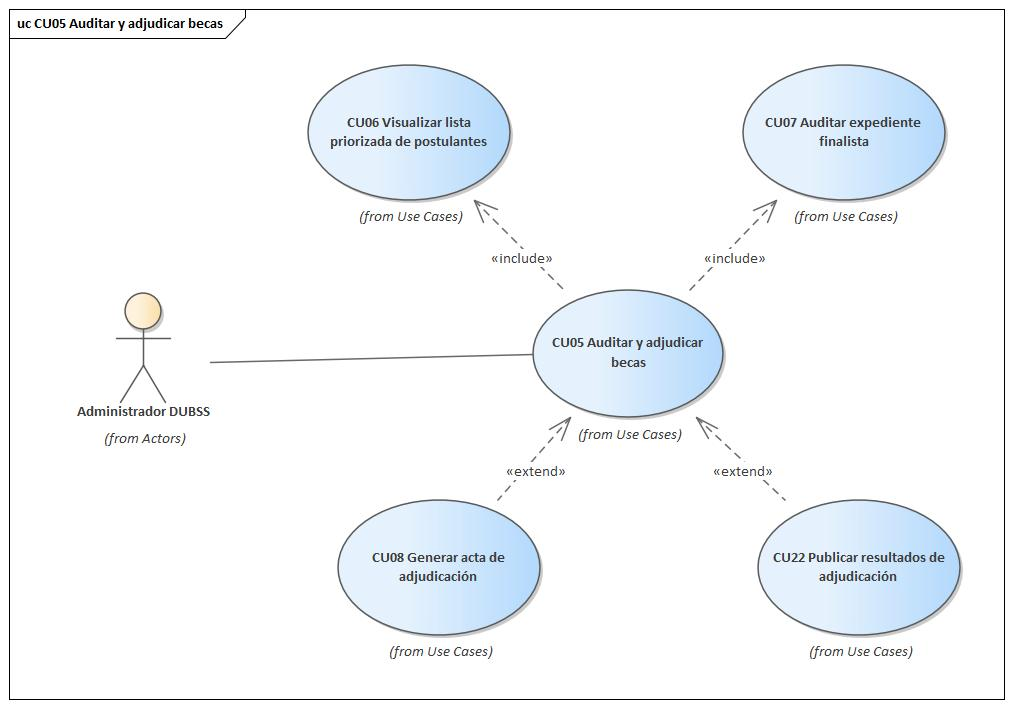
\includegraphics[width=0.8\textwidth,height=0.4\textheight,keepaspectratio]{images/064_CU05_Auditar_Adjudicar_Becas.jpg}

\smallskip
\noindent\raggedright\textit{Nota.} Elaboración propia.
\end{figure}

\refstepcounter{table}\label{tab:detalle_cu05}
\addcontentsline{lot}{table}{\protect\numberline{\thetable}Detalle del CU-05: Auditar y adjudicar becas}
\noindent\textbf{Tabla~\thetable}\par\nopagebreak
\noindent\textit{Detalle del CU-05: Auditar y adjudicar becas}\par\nopagebreak
\begingroup\small\linespread{1}\selectfont
\begin{longtable}{>{\raggedright\arraybackslash}p{2.9cm} >{\raggedright\arraybackslash}p{12.6cm}}
\toprule
\textbf{Caso de Uso} & \textbf{CU-05. Auditar y adjudicar becas} \\
\midrule
\endfirsthead
\toprule
\textbf{Caso de Uso} & \textbf{CU-05. Auditar y adjudicar becas} \\
\midrule
\endhead
\endfoot
\bottomrule
\multicolumn{2}{l}{\textit{Nota.} Elaboración propia.} \\
\endlastfoot
\textbf{Propósito} & Permitir al Administrador DUBSS conducir el proceso de selección de los beneficiarios: identificar a los finalistas mejor puntuados, auditar sus expedientes y registrar la decisión de adjudicar o no adjudicar la Beca Comedor a cada uno de ellos. \\
\midrule
\textbf{Descripción} & Este caso de uso describe el proceso completo de auditoría y adjudicación de una convocatoria. A partir de la lista priorizada por el puntaje de vulnerabilidad (se incluye el CU-06), el Administrador DUBSS selecciona a los finalistas, audita el expediente de cada uno (se incluye el CU-07) y registra la decisión de adjudicación, que queda asociada a la postulación junto con el puntaje total (puntaje de la IA más el puntaje académico de la última auditoría), el usuario que decide y la fecha de adjudicación. El CU-08 lo extiende para generar el acta de adjudicación y el CU-22 para publicar los resultados. Respalda el RF-04. \\
\midrule
\textbf{Actores} & Administrador DUBSS. \\
\midrule
\textbf{Actor Iniciador} & Administrador DUBSS. \\
\midrule
\textbf{Precondición} & \vspace{-\baselineskip}\begin{cuvin}
    \item El Administrador DUBSS está autenticado en el sistema (CU-01) con el rol Administrador DUBSS.
    \item La convocatoria de la gestión académica vigente se encuentra cerrada a la recepción de postulaciones (CU-13).
    \item Existen postulaciones en estado «calificada», con puntaje de vulnerabilidad vigente (CU-03).
    \item La convocatoria tiene registrados el número de cupos y el puntaje mínimo requerido (valores por definir con la DUBSS) y, opcionalmente, la cantidad de finalistas, que solo ve el Administrador DUBSS (CU-13).
\end{cuvin} \\
\midrule
\textbf{Proceso} & \textbf{Flujo principal.}
\begin{cupasos}
    \item El Administrador DUBSS selecciona la opción «Auditoría y adjudicación» y la convocatoria a procesar.
    \item El sistema muestra el panel de la convocatoria (cupos, adjudicados, no adjudicados, cupos disponibles y puntaje mínimo) y su lista priorizada de postulantes (se incluye el CU-06).
    \item El Administrador DUBSS selecciona como finalistas a los postulantes mejor puntuados. El sistema propone la cantidad de finalistas configurada en la convocatoria y el Administrador puede ajustarla antes de confirmar.
    \item El sistema registra a cada finalista con la posición que ocupa en la lista priorizada completa, sin repetir a los ya seleccionados.
    \item El Administrador DUBSS audita el expediente de cada finalista (se incluye el CU-07).
    \item El sistema muestra la lista de finalistas con el resultado de su auditoría y el número de cupos disponibles.
    \item El Administrador DUBSS abre el expediente de un finalista auditado y registra su decisión: adjudicar o no adjudicar la beca. Si no adjudica, debe escribir un motivo (hasta 500 caracteres) y confirmar en una ventana que muestra el nombre, el puntaje total y los cupos disponibles.
    \item El sistema valida la decisión y registra la adjudicación con su resultado, el puntaje total de la postulación (puntaje de la IA más el puntaje académico de la última auditoría), el usuario que decide y la fecha de adjudicación.
    \item El sistema actualiza el estado de la postulación a «adjudicada» o «no adjudicada», registra el cambio en el historial de la postulación (con el motivo, si no adjudica) y en la bitácora, y actualiza el número de cupos disponibles, todo en una misma operación. No avisa al postulante: este se entera al publicar los resultados (CU-22).
    \item Los pasos 7 a 9 se repiten hasta decidir sobre todos los finalistas.
\end{cupasos} \\
 & \textbf{Flujos alternativos.}
\begin{cuvin}
    \item A1 (paso 2): si la convocatoria no tiene postulaciones calificadas, el sistema informa que no existen postulaciones para auditar.
    \item A2 (paso 7): si el finalista no tiene ninguna auditoría, el sistema no permite ninguna decisión (409, ERR\_ADJ\_02); si la última auditoría no es «validado», no permite adjudicarle la beca (409, ERR\_ADJ\_02) pero sí no adjudicar.
    \item A3 (paso 7): si el puntaje total de la postulación (IA más académico de la última auditoría) no alcanza el puntaje mínimo requerido, el sistema no permite adjudicarle la beca (409, ERR\_ADJ\_03).
    \item A4 (paso 7): si los cupos de la convocatoria están agotados, el sistema no permite registrar nuevas adjudicaciones (409, ERR\_ADJ\_04) y solo admite la decisión de no adjudicar.
    \item A5 (paso 10): una vez decididas todas las adjudicaciones, el Administrador DUBSS puede publicar los resultados (CU-22) y, una vez publicados, generar el acta de adjudicación (CU-08).
    \item A6 (paso 7): si los resultados de la convocatoria ya fueron publicados (CU-22) o la postulación ya no está «calificada», el sistema no registra ni modifica decisiones (409, ERR\_ADJ\_01).
    \item A7 (paso 8): si la petición llega duplicada (doble clic o reintento), solo se registra una decisión; la segunda recibe el 409 ERR\_ADJ\_01, sin clave de idempotencia.
    \item A8 (pasos 1 y 7): si la convocatoria no está cerrada o no tiene cupos o puntaje mínimo definidos, el sistema no permite seleccionar finalistas ni decidir (409, ERR\_ADJ\_05).
\end{cuvin} \\
\midrule
\textbf{Postcondición} & \vspace{-\baselineskip}\begin{cuvin}
    \item Cada finalista decidido tiene una adjudicación registrada con su resultado, puntaje final, responsable y fecha de adjudicación.
    \item La postulación queda en estado «adjudicada» o «no adjudicada» y el cambio queda registrado en el historial de la postulación y en la bitácora.
\end{cuvin} \\
\midrule
\textbf{Excepciones} & \vspace{-\baselineskip}\begin{cuvin}
    \item Autenticación inválida o sesión expirada.
    \item Falta de permisos suficientes (el usuario no tiene el rol Administrador DUBSS).
    \item Cupos de la convocatoria agotados.
    \item Error de conexión con el servidor o la base de datos al registrar la adjudicación.
\end{cuvin} \\
\end{longtable}
\endgroup
\addtocounter{table}{-1}

\subsubsection{5.4.6. CU-06 Visualizar lista priorizada de postulantes}\label{sec:cap5_cu06}

\begin{figure}[H]
\caption{Diagrama de contexto del CU-06}
\label{fig:ctx_cu06}
\centering
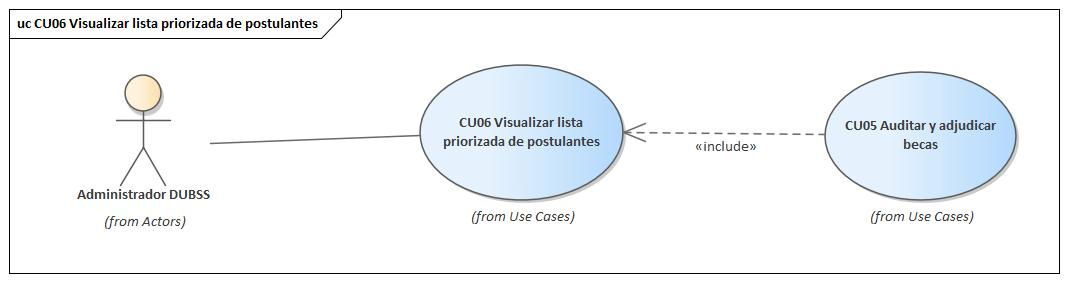
\includegraphics[width=0.8\textwidth,height=0.4\textheight,keepaspectratio]{images/065_CU06_Visualizar_Lista_Priorizada_Postulantes.jpg}

\smallskip
\noindent\raggedright\textit{Nota.} Elaboración propia.
\end{figure}

\refstepcounter{table}\label{tab:detalle_cu06}
\addcontentsline{lot}{table}{\protect\numberline{\thetable}Detalle del CU-06: Visualizar lista priorizada de postulantes}
\noindent\textbf{Tabla~\thetable}\par\nopagebreak
\noindent\textit{Detalle del CU-06: Visualizar lista priorizada de postulantes}\par\nopagebreak
\begingroup\small\linespread{1}\selectfont
\begin{longtable}{>{\raggedright\arraybackslash}p{2.9cm} >{\raggedright\arraybackslash}p{12.6cm}}
\toprule
\textbf{Caso de Uso} & \textbf{CU-06. Visualizar lista priorizada de postulantes} \\
\midrule
\endfirsthead
\toprule
\textbf{Caso de Uso} & \textbf{CU-06. Visualizar lista priorizada de postulantes} \\
\midrule
\endhead
\endfoot
\bottomrule
\multicolumn{2}{l}{\textit{Nota.} Elaboración propia.} \\
\endlastfoot
\textbf{Propósito} & Presentar al Administrador DUBSS las postulaciones de una convocatoria ordenadas de mayor a menor puntaje de vulnerabilidad, para que la auditoría se concentre únicamente en los postulantes mejor puntuados. \\
\midrule
\textbf{Descripción} & Este caso de uso describe cómo el sistema construye y muestra la lista priorizada de postulantes de una convocatoria a partir de las postulaciones en estado «calificada» y de su puntaje vigente calculado por el módulo de IA (CU-03). La lista no se almacena como tal: se obtiene mediante una consulta ordenada y paginada, por lo que siempre refleja el último puntaje calculado. Es incluido por el CU-05. Respalda el RF-04. \\
\midrule
\textbf{Actores} & Administrador DUBSS. \\
\midrule
\textbf{Actor Iniciador} & Administrador DUBSS. \\
\midrule
\textbf{Precondición} & \vspace{-\baselineskip}\begin{cuvin}
    \item El Administrador DUBSS está autenticado en el sistema (CU-01) con el rol Administrador DUBSS.
    \item Existe al menos una convocatoria registrada (CU-13).
    \item Las postulaciones de la convocatoria fueron precalificadas por el módulo de IA (CU-03).
\end{cuvin} \\
\midrule
\textbf{Proceso} & \textbf{Flujo principal.}
\begin{cupasos}
    \item El Administrador DUBSS selecciona la opción «Lista priorizada» (o accede a ella desde el CU-05).
    \item El sistema muestra las convocatorias disponibles.
    \item El Administrador DUBSS selecciona una convocatoria.
    \item El sistema obtiene las postulaciones de la convocatoria en estado «calificada» y su puntaje de vulnerabilidad vigente.
    \item El sistema ordena las postulaciones de mayor a menor puntaje y muestra la lista paginada con: posición, código de postulación, nombre, CI y carrera del postulante, puntaje y fecha de cálculo.
    \item El Administrador DUBSS revisa la lista y, si lo desea, selecciona una postulación para continuar con su auditoría (CU-05).
\end{cupasos} \\
 & \textbf{Flujos alternativos.}
\begin{cuvin}
    \item A1 (paso 4): si la convocatoria no tiene postulaciones calificadas, el sistema muestra un mensaje informativo.
    \item A2 (paso 6): si el Administrador DUBSS aplica un filtro o criterio de ordenamiento (por ejemplo, por carrera), el sistema vuelve a consultar las postulaciones y los puntajes y muestra la lista resultante.
    \item A3 (paso 5): si dos o más postulaciones tienen el mismo puntaje, el sistema aplica el criterio de desempate vigente (por definir con la DUBSS).
    \item A4 (paso 4): las postulaciones en estado «pendiente», «devuelta», «archivada», «adjudicada» o «no adjudicada» no forman parte de la lista priorizada activa; el sistema informa cuántas postulaciones siguen pendientes de precalificación.
    \item A5 (paso 6): si el Administrador DUBSS solicita exportar la lista, el sistema genera un documento PDF con la lista priorizada de la convocatoria (respetando el filtro u orden aplicado), registra la exportación en la bitácora (CU-25) y ofrece la descarga del archivo.
\end{cuvin} \\
\midrule
\textbf{Postcondición} & \vspace{-\baselineskip}\begin{cuvin}
    \item El Administrador DUBSS visualiza la lista priorizada de la convocatoria; la consulta no modifica ningún dato de las postulaciones ni de los puntajes.
    \item Si exportó la lista a PDF (A5), queda un registro de la exportación en la bitácora.
\end{cuvin} \\
\midrule
\textbf{Excepciones} & \vspace{-\baselineskip}\begin{cuvin}
    \item Autenticación inválida o sesión expirada.
    \item Falta de permisos suficientes (el usuario no tiene el rol Administrador DUBSS).
    \item Error de conexión con el servidor o la base de datos.
    \item Tiempo de respuesta excedido al consultar un volumen alto de postulaciones (hasta 20,000 por gestión).
\end{cuvin} \\
\end{longtable}
\endgroup
\addtocounter{table}{-1}

\subsubsection{5.4.7. CU-07 Auditar expediente finalista}\label{sec:cap5_cu07}

\begin{figure}[H]
\caption{Diagrama de contexto del CU-07}
\label{fig:ctx_cu07}
\centering
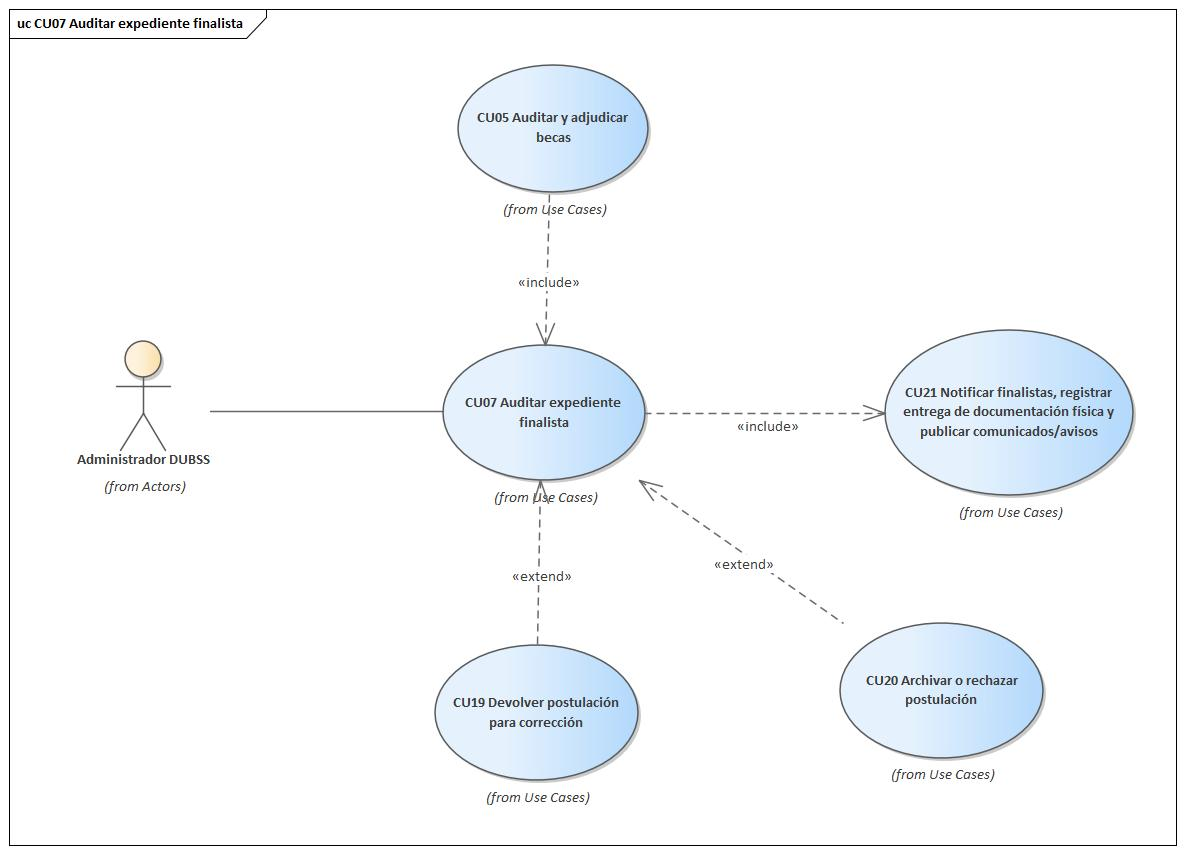
\includegraphics[width=0.8\textwidth,height=0.4\textheight,keepaspectratio]{images/066_CU07_Auditar_Expediente_Finalista.jpg}

\smallskip
\noindent\raggedright\textit{Nota.} Elaboración propia.
\end{figure}

\refstepcounter{table}\label{tab:detalle_cu07}
\addcontentsline{lot}{table}{\protect\numberline{\thetable}Detalle del CU-07: Auditar expediente finalista}
\noindent\textbf{Tabla~\thetable}\par\nopagebreak
\noindent\textit{Detalle del CU-07: Auditar expediente finalista}\par\nopagebreak
\begingroup\small\linespread{1}\selectfont
\begin{longtable}{>{\raggedright\arraybackslash}p{2.9cm} >{\raggedright\arraybackslash}p{12.6cm}}
\toprule
\textbf{Caso de Uso} & \textbf{CU-07. Auditar expediente finalista} \\
\midrule
\endfirsthead
\toprule
\textbf{Caso de Uso} & \textbf{CU-07. Auditar expediente finalista} \\
\midrule
\endhead
\endfoot
\bottomrule
\multicolumn{2}{l}{\textit{Nota.} Elaboración propia.} \\
\endlastfoot
\textbf{Propósito} & Permitir al Administrador DUBSS revisar el expediente de un finalista, cotejar su documentación física con la digital y registrar el resultado de la auditoría junto con su puntaje de rendimiento académico. \\
\midrule
\textbf{Descripción} & Este caso de uso describe cómo el Administrador DUBSS audita el expediente de un postulante seleccionado como finalista. El sistema presenta los datos de la postulación, las respuestas socioeconómicas, los documentos digitales adjuntos y el puntaje de la inteligencia artificial (hasta 70 puntos); el Administrador coteja esa información con la documentación física entregada por el finalista y registra el resultado de la auditoría (validado, observado o no válido) con sus observaciones (hasta 500 caracteres) y, si es validado, el puntaje de rendimiento académico (0 a 30), con lo que el sistema muestra el total (hasta 100). El finalista se elige desde la lista de finalistas del CU-21 (columna «Auditoría») y solo se audita si su entrega física está registrada y su postulación sigue «calificada». Al registrar la auditoría se avisa al postulante. Incluye la notificación al finalista y el registro de la entrega de su documentación física (CU-21). El CU-19 lo extiende para devolver la postulación y el CU-20 para archivarla o rechazarla. Es incluido por el CU-05. Respalda el RF-04. \\
\midrule
\textbf{Actores} & Administrador DUBSS. \\
\midrule
\textbf{Actor Iniciador} & Administrador DUBSS. \\
\midrule
\textbf{Precondición} & \vspace{-\baselineskip}\begin{cuvin}
    \item El Administrador DUBSS está autenticado en el sistema (CU-01) con el rol Administrador DUBSS.
    \item La postulación fue seleccionada como finalista en el CU-05 y se encuentra en estado «calificada».
    \item Los documentos digitales de la postulación están almacenados en MinIO (CU-16).
    \item La entrega de la documentación física del finalista está registrada (CU-21).
\end{cuvin} \\
\midrule
\textbf{Proceso} & \textbf{Flujo principal.}
\begin{cupasos}
    \item El Administrador DUBSS selecciona un finalista de la lista de finalistas de la convocatoria.
    \item El sistema muestra el expediente del finalista: datos del postulante, respuestas socioeconómicas, documentos digitales adjuntos, puntaje de vulnerabilidad de la IA con su desglose y estado de la entrega de la documentación física.
    \item El sistema notifica al finalista el plazo y los documentos físicos que debe presentar y registra la recepción de dicha documentación (se incluye el CU-21).
    \item El Administrador DUBSS coteja la documentación física entregada con los documentos digitales y los datos declarados.
    \item El Administrador DUBSS registra el resultado de la auditoría (validado, observado o no válido), sus observaciones (hasta 500 caracteres) y, si el resultado es «validado», el puntaje de rendimiento académico (0 a 30).
    \item El sistema valida los datos, registra la auditoría con su resultado, observaciones, puntaje académico, auditor y fecha, y deja constancia en la bitácora.
    \item El sistema avisa al postulante el resultado de la auditoría y muestra el expediente como auditado con el puntaje de la IA, el puntaje académico y el total; si el resultado es «validado», el finalista queda habilitado para la decisión de adjudicación (CU-05).
\end{cupasos} \\
 & \textbf{Flujos alternativos.}
\begin{cuvin}
    \item A1 (paso 3): si el finalista no entrega la documentación física dentro del plazo (por definir con la DUBSS), el Administrador DUBSS puede archivar la postulación (CU-20).
    \item A2 (paso 5): si el expediente presenta defectos subsanables, el Administrador DUBSS puede devolver la postulación para su corrección (CU-19).
    \item A3 (paso 5): si la documentación no es válida o la postulación no procede, el Administrador DUBSS puede archivarla o rechazarla (CU-20).
    \item A4 (paso 2): si un documento digital no puede recuperarse del almacenamiento de archivos, el sistema informa el error y permite reintentar la descarga.
    \item A5 (paso 6): si el expediente ya tenía una auditoría (por ejemplo, después de una devolución), el sistema registra la nueva auditoría y conserva las anteriores; una postulación devuelta y reenviada recorre de nuevo el flujo finalista, entrega física y auditoría.
    \item A6 (paso 1): si la entrega física del finalista no está registrada, el sistema rechaza la auditoría (conflicto) e indica registrar primero la entrega (CU-21).
    \item A7 (paso 6): si la postulación ya no está en estado «calificada» (por ejemplo, otro administrador la devolvió o archivó), el sistema rechaza la auditoría (conflicto).
    \item A8 (paso 6): si los datos son inválidos (observaciones de más de 500 caracteres, falta el puntaje académico en un resultado «validado» o puntaje fuera del rango de 0 a 30), el sistema informa el error y no registra la auditoría.
    \item A9 (paso 6): si la misma petición se repite (doble clic o reintento), el sistema la trata de forma idempotente y no duplica la auditoría.
\end{cuvin} \\
\midrule
\textbf{Postcondición} & \vspace{-\baselineskip}\begin{cuvin}
    \item El expediente del finalista tiene registrada una auditoría con su resultado, observaciones, puntaje académico (si es validado), auditor y fecha.
    \item El postulante recibe el aviso del resultado de la auditoría.
    \item La acción queda registrada en la bitácora.
\end{cuvin} \\
\midrule
\textbf{Excepciones} & \vspace{-\baselineskip}\begin{cuvin}
    \item Autenticación inválida o sesión expirada.
    \item Falta de permisos suficientes (el usuario no tiene el rol Administrador DUBSS).
    \item Error al recuperar los documentos desde MinIO.
    \item Entrega física no registrada o postulación que ya no está calificada (conflicto de estado).
    \item Error de conexión con el servidor o la base de datos al registrar la auditoría.
\end{cuvin} \\
\end{longtable}
\endgroup
\addtocounter{table}{-1}

\subsubsection{5.4.8. CU-08 Generar acta de adjudicación}\label{sec:cap5_cu08}

\begin{figure}[H]
\caption{Diagrama de contexto del CU-08}
\label{fig:ctx_cu08}
\centering
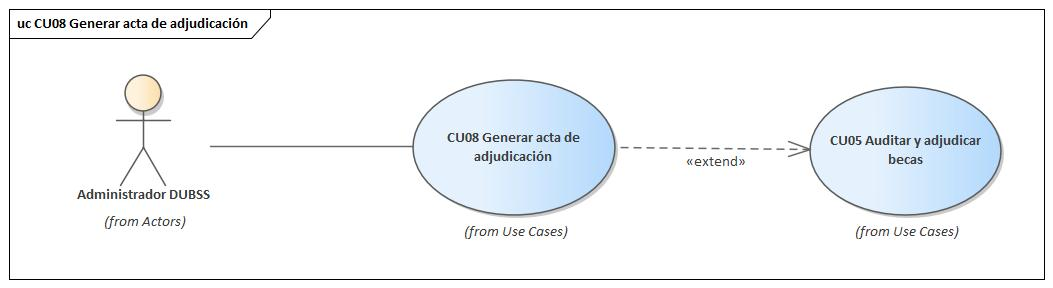
\includegraphics[width=0.8\textwidth,height=0.4\textheight,keepaspectratio]{images/067_CU08_Generar_Acta_Adjudicacion.jpg}

\smallskip
\noindent\raggedright\textit{Nota.} Elaboración propia.
\end{figure}

\refstepcounter{table}\label{tab:detalle_cu08}
\addcontentsline{lot}{table}{\protect\numberline{\thetable}Detalle del CU-08: Generar acta de adjudicación}
\noindent\textbf{Tabla~\thetable}\par\nopagebreak
\noindent\textit{Detalle del CU-08: Generar acta de adjudicación}\par\nopagebreak
\begingroup\small\linespread{1}\selectfont
\begin{longtable}{>{\raggedright\arraybackslash}p{2.9cm} >{\raggedright\arraybackslash}p{12.6cm}}
\toprule
\textbf{Caso de Uso} & \textbf{CU-08. Generar acta de adjudicación} \\
\midrule
\endfirsthead
\toprule
\textbf{Caso de Uso} & \textbf{CU-08. Generar acta de adjudicación} \\
\midrule
\endhead
\endfoot
\bottomrule
\multicolumn{2}{l}{\textit{Nota.} Elaboración propia.} \\
\endlastfoot
\textbf{Propósito} & Generar el acta oficial que deja constancia de los resultados de la adjudicación de la Beca Comedor de una convocatoria. \\
\midrule
\textbf{Descripción} & Este caso de uso describe cómo el Administrador DUBSS genera, una vez publicados los resultados de una convocatoria (CU-22), el acta de adjudicación en formato PDF con la lista de beneficiarios adjudicados y su puntaje final. Antes de generarla puede ver una vista previa con el número «borrador». El acta se almacena en MinIO, se registra con un número único automático, es definitiva (una sola por convocatoria, no se regenera ni se elimina) y puede consultarse y descargarse después mediante una dirección temporal firmada. El formato y el contenido oficial del acta están por definir con la DUBSS. Extiende el CU-05. Respalda el RF-04. \\
\midrule
\textbf{Actores} & Administrador DUBSS. \\
\midrule
\textbf{Actor Iniciador} & Administrador DUBSS. \\
\midrule
\textbf{Precondición} & \vspace{-\baselineskip}\begin{cuvin}
    \item El Administrador DUBSS está autenticado en el sistema (CU-01) con el rol Administrador DUBSS.
    \item Los resultados de la convocatoria ya fueron publicados (CU-22) y la convocatoria está «publicada».
    \item Para generar, la convocatoria aún no tiene acta; para consultar o descargar, ya la tiene.
\end{cuvin} \\
\midrule
\textbf{Proceso} & \textbf{Flujo principal A: generar el acta.}
\begin{cupasos}
    \item El Administrador DUBSS entra a «Actas», elige una convocatoria con resultados publicados y sin acta y, si lo desea, pulsa «Vista previa».
    \item El Administrador DUBSS pulsa «Generar PDF» y confirma en una ventana que avisa que el acta es definitiva.
    \item El sistema verifica que la convocatoria exista, que sus resultados estén publicados y que no tenga acta.
    \item El sistema obtiene los adjudicados de la convocatoria con nombre y apellido, CI, carrera y puntaje final, y asigna el número de acta.
    \item El sistema genera el PDF con el número, la fecha, los datos de la convocatoria y de la gestión académica y la lista de adjudicados, y lo almacena en MinIO.
    \item El sistema registra el acta con su número, la ruta del archivo, el usuario que la genera y la fecha de generación, y deja constancia en la bitácora, en una misma operación.
    \item El sistema muestra el acta generada y permite descargarla e imprimirla.
\end{cupasos} \\
 & \textbf{Flujo principal B: consultar el acta.}
\begin{cupasos}
    \item El Administrador DUBSS entra a «Actas» y pulsa «Descargar» en el acta que desea (o elige una convocatoria que ya la tiene).
    \item El sistema obtiene el acta registrada y comprueba que el archivo esté disponible.
    \item El sistema anota la descarga en la bitácora y entrega una dirección temporal firmada (vigente 5 minutos) para abrir el PDF.
\end{cupasos} \\
 & \textbf{Flujos alternativos.}
\begin{cuvin}
    \item A1 (flujo A, paso 3): si los resultados de la convocatoria no están publicados, el sistema no genera el acta (409, ERR\_ACT\_01) e indica que primero hay que publicarlos (CU-22).
    \item A2 (flujo A, paso 3): si la convocatoria ya tiene acta, el sistema no genera otra (409, ERR\_ACT\_02) y muestra la existente; un doble clic recibe el mismo 409.
    \item A3 (flujo A, paso 5): si falla la generación del PDF o el guardado en MinIO, el sistema no registra el acta ni la bitácora y permite reintentar.
    \item A4 (flujo B, paso 2): si la convocatoria aún no tiene acta, el sistema lo informa (404, ERR\_ACT\_03); si el acta está registrada pero su archivo no está en el almacenamiento, informa que hay que avisar a soporte (404, ERR\_ACT\_04).
\end{cuvin} \\
\midrule
\textbf{Postcondición} & \vspace{-\baselineskip}\begin{cuvin}
    \item El acta de adjudicación de la convocatoria queda almacenada en MinIO y registrada con su número, responsable y fecha de generación; es definitiva y no se regenera.
    \item La generación del acta queda registrada en la bitácora.
\end{cuvin} \\
\midrule
\textbf{Excepciones} & \vspace{-\baselineskip}\begin{cuvin}
    \item Autenticación inválida o sesión expirada.
    \item Falta de permisos suficientes (el usuario no tiene el rol Administrador DUBSS).
    \item Error al generar el documento PDF.
    \item Error al almacenar el archivo en MinIO.
    \item Error de conexión con el servidor o la base de datos.
\end{cuvin} \\
\end{longtable}
\endgroup
\addtocounter{table}{-1}

\subsubsection{5.4.9. CU-09 Generar planilla de asistencia}\label{sec:cap5_cu09}

\begin{figure}[H]
\caption{Diagrama de contexto del CU-09}
\label{fig:ctx_cu09}
\centering
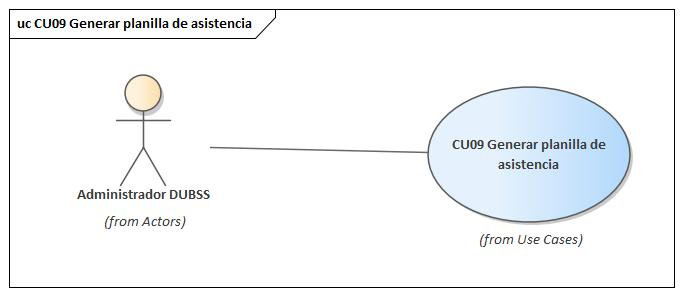
\includegraphics[width=0.8\textwidth,height=0.4\textheight,keepaspectratio]{images/068_CU09_Generar_Planilla_Asistencia.jpg}

\smallskip
\noindent\raggedright\textit{Nota.} Elaboración propia.
\end{figure}

\refstepcounter{table}\label{tab:detalle_cu09}
\addcontentsline{lot}{table}{\protect\numberline{\thetable}Detalle del CU-09: Generar planilla de asistencia}
\noindent\textbf{Tabla~\thetable}\par\nopagebreak
\noindent\textit{Detalle del CU-09: Generar planilla de asistencia}\par\nopagebreak
\begingroup\small\linespread{1}\selectfont
\begin{longtable}{>{\raggedright\arraybackslash}p{2.9cm} >{\raggedright\arraybackslash}p{12.6cm}}
\toprule
\textbf{Caso de Uso} & \textbf{CU-09. Generar planilla de asistencia} \\
\midrule
\endfirsthead
\toprule
\textbf{Caso de Uso} & \textbf{CU-09. Generar planilla de asistencia} \\
\midrule
\endhead
\endfoot
\bottomrule
\multicolumn{2}{l}{\textit{Nota.} Elaboración propia.} \\
\endlastfoot
\textbf{Propósito} & Generar planillas de asistencia imprimibles, a partir del padrón de becados vigente, que sirvan como respaldo físico del uso del beneficio ante las auditorías. \\
\midrule
\textbf{Descripción} & Este caso de uso describe cómo el Administrador DUBSS genera, para un periodo determinado, la planilla de asistencia de los becados vigentes de la convocatoria. La planilla se genera en formato PDF, lista para su impresión, con los espacios para la firma de cada becado y la fotocopia de su carnet, tal como lo exigen las auditorías; se almacena en MinIO y queda disponible para su consulta y para el cotejo con el registro digital (CU-11). Respalda el RF-05. \\
\midrule
\textbf{Actores} & Administrador DUBSS. \\
\midrule
\textbf{Actor Iniciador} & Administrador DUBSS. \\
\midrule
\textbf{Precondición} & \vspace{-\baselineskip}\begin{cuvin}
    \item El Administrador DUBSS está autenticado en el sistema (CU-01) con el rol Administrador DUBSS.
    \item Existe un padrón de becados vigentes para la convocatoria (CU-23).
\end{cuvin} \\
\midrule
\textbf{Proceso} & \textbf{Flujo principal A: generar una planilla.}
\begin{cupasos}
    \item El Administrador DUBSS selecciona la opción «Planillas de asistencia» y la convocatoria correspondiente.
    \item El sistema solicita el periodo de la planilla (fecha desde y fecha hasta).
    \item El Administrador DUBSS ingresa el periodo y confirma la generación.
    \item El sistema valida que la fecha final no sea anterior a la inicial y que el periodo esté comprendido en la gestión académica.
    \item El sistema obtiene las becas en estado vigente de la convocatoria.
    \item El sistema genera la planilla en formato PDF con la lista de becados (nombre, CI y carrera) y los espacios para la firma y la fotocopia del carnet de cada uno (formato por definir con la DUBSS).
    \item El sistema almacena el PDF en MinIO y registra la planilla con su periodo, la ruta del archivo, el usuario que la genera y la fecha de generación.
    \item El sistema muestra la planilla generada para su descarga e impresión.
\end{cupasos} \\
 & \textbf{Flujo principal B: consultar planillas.}
\begin{cupasos}
    \item El Administrador DUBSS selecciona la opción «Consultar planillas» de la convocatoria.
    \item El sistema muestra la lista de planillas generadas con su periodo y fecha de generación, y permite descargar cualquiera de ellas.
\end{cupasos} \\
 & \textbf{Flujos alternativos.}
\begin{cuvin}
    \item A1 (flujo A, paso 4): si el periodo es inválido, el sistema lo indica y permite corregirlo.
    \item A2 (flujo A, paso 5): si la convocatoria no tiene becas vigentes, el sistema no genera la planilla e informa el motivo.
    \item A3 (flujo A, paso 7): si ocurre un error al almacenar el PDF, el sistema no registra la planilla y permite reintentar.
    \item A4 (flujo A, paso 5): la planilla refleja el padrón vigente al momento de su generación; los cambios posteriores en el padrón (CU-23) se reflejan en las planillas que se generen después.
\end{cuvin} \\
\midrule
\textbf{Postcondición} & \vspace{-\baselineskip}\begin{cuvin}
    \item La planilla de asistencia queda almacenada en MinIO y registrada con su periodo, responsable y fecha de generación.
    \item La planilla queda disponible para su impresión y para el cotejo con el registro digital (CU-11).
\end{cuvin} \\
\midrule
\textbf{Excepciones} & \vspace{-\baselineskip}\begin{cuvin}
    \item Autenticación inválida o sesión expirada.
    \item Falta de permisos suficientes (el usuario no tiene el rol Administrador DUBSS).
    \item Error al generar el documento PDF.
    \item Error al almacenar el archivo en MinIO.
    \item Error de conexión con el servidor o la base de datos.
\end{cuvin} \\
\end{longtable}
\endgroup
\addtocounter{table}{-1}

\subsubsection{5.4.10. CU-10 Registrar asistencia digital}\label{sec:cap5_cu10}

\begin{figure}[H]
\caption{Diagrama de contexto del CU-10}
\label{fig:ctx_cu10}
\centering
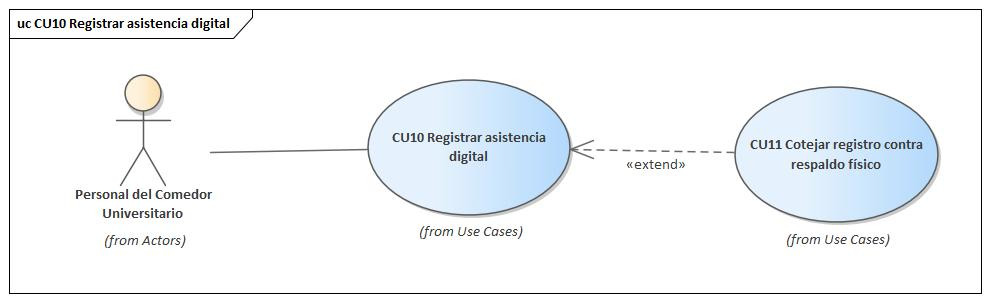
\includegraphics[width=0.8\textwidth,height=0.4\textheight,keepaspectratio]{images/069_CU10_Registrar_Asistencia_Digital.jpg}

\smallskip
\noindent\raggedright\textit{Nota.} Elaboración propia.
\end{figure}

\refstepcounter{table}\label{tab:detalle_cu10}
\addcontentsline{lot}{table}{\protect\numberline{\thetable}Detalle del CU-10: Registrar asistencia digital}
\noindent\textbf{Tabla~\thetable}\par\nopagebreak
\noindent\textit{Detalle del CU-10: Registrar asistencia digital}\par\nopagebreak
\begingroup\small\linespread{1}\selectfont
\begin{longtable}{>{\raggedright\arraybackslash}p{2.9cm} >{\raggedright\arraybackslash}p{12.6cm}}
\toprule
\textbf{Caso de Uso} & \textbf{CU-10. Registrar asistencia digital} \\
\midrule
\endfirsthead
\toprule
\textbf{Caso de Uso} & \textbf{CU-10. Registrar asistencia digital} \\
\midrule
\endhead
\endfoot
\bottomrule
\multicolumn{2}{l}{\textit{Nota.} Elaboración propia.} \\
\endlastfoot
\textbf{Propósito} & Registrar digitalmente la asistencia diaria de cada becado al Comedor Universitario, una vez verificada su identidad por el personal del comedor. \\
\midrule
\textbf{Descripción} & Este caso de uso describe cómo el Personal del Comedor Universitario registra, desde la aplicación móvil, la asistencia diaria de un becado. El sistema no cuenta con un mecanismo biométrico propio: la verificación de identidad la realiza el comedor por sus propios medios y el sistema solo registra su resultado. Se admite un único registro por becado y por día, de modo que las peticiones duplicadas no generan registros adicionales. El CU-11 lo extiende para cotejar el registro digital contra el respaldo físico. Respalda el RF-05. \\
\midrule
\textbf{Actores} & Personal del Comedor Universitario. \\
\midrule
\textbf{Actor Iniciador} & Personal del Comedor Universitario. \\
\midrule
\textbf{Precondición} & \vspace{-\baselineskip}\begin{cuvin}
    \item El Personal del Comedor Universitario está autenticado en la aplicación móvil (CU-01) con el rol Personal del Comedor Universitario.
    \item Existe un padrón de becados vigentes (CU-23).
    \item El personal del comedor verificó la identidad del becado por los medios propios del comedor.
\end{cuvin} \\
\midrule
\textbf{Proceso} & \textbf{Flujo principal.}
\begin{cupasos}
    \item El Personal del Comedor Universitario selecciona la opción «Registrar asistencia» en la aplicación móvil.
    \item El sistema muestra la fecha actual y solicita el CI del becado.
    \item El Personal del Comedor Universitario ingresa el CI del becado.
    \item El sistema busca la beca asociada al CI y verifica que se encuentre en estado vigente.
    \item El sistema muestra los datos del becado: nombre, CI, carrera y estado de la beca.
    \item El Personal del Comedor Universitario confirma el registro de la asistencia.
    \item El sistema verifica que no exista un registro de asistencia de esa beca en la fecha actual.
    \item El sistema registra la asistencia con la fecha, la hora de registro y el usuario que la registra.
    \item El sistema confirma el registro y queda listo para el siguiente becado.
\end{cupasos} \\
 & \textbf{Flujos alternativos.}
\begin{cuvin}
    \item A1 (paso 4): si el CI no corresponde a ningún becado, el sistema informa que el estudiante no figura en el padrón de becados.
    \item A2 (paso 4): si la beca se encuentra suspendida o dada de baja, el sistema no permite el registro e informa el estado de la beca.
    \item A3 (paso 7): si la asistencia del día ya fue registrada, el sistema no crea un nuevo registro e informa la hora del registro existente (idempotencia).
    \item A4 (paso 9): durante una auditoría, el Administrador DUBSS puede cotejar los registros digitales contra la planilla física firmada (CU-11).
\end{cuvin} \\
\midrule
\textbf{Postcondición} & \vspace{-\baselineskip}\begin{cuvin}
    \item La asistencia del becado queda registrada una sola vez para la fecha, con la hora y el usuario que la registró.
    \item El registro queda disponible para la consulta del becado (CU-24), el cotejo (CU-11) y los indicadores de BI (CU-12).
\end{cuvin} \\
\midrule
\textbf{Excepciones} & \vspace{-\baselineskip}\begin{cuvin}
    \item Autenticación inválida o sesión expirada.
    \item Falta de permisos suficientes (el usuario no tiene el rol Personal del Comedor Universitario).
    \item Becado inexistente o beca no vigente.
    \item Error de conexión con el servidor o la base de datos (la asistencia no se registra y debe reintentarse).
\end{cuvin} \\
\end{longtable}
\endgroup
\addtocounter{table}{-1}

\subsubsection{5.4.11. CU-11 Cotejar registro contra respaldo físico}\label{sec:cap5_cu11}

\begin{figure}[H]
\caption{Diagrama de contexto del CU-11}
\label{fig:ctx_cu11}
\centering
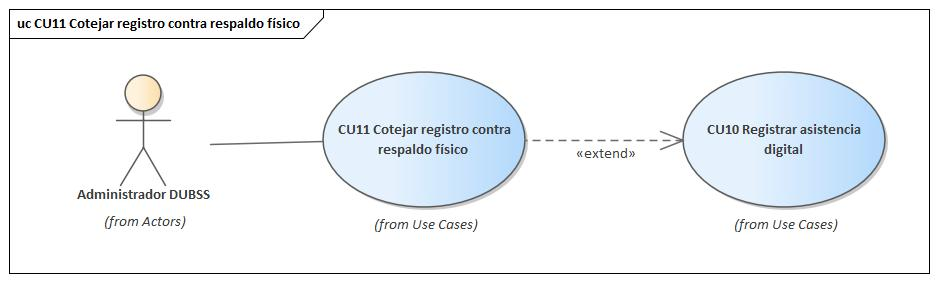
\includegraphics[width=0.8\textwidth,height=0.4\textheight,keepaspectratio]{images/070_CU11_Cotejar_Registro_Respaldo_Fisico.jpg}

\smallskip
\noindent\raggedright\textit{Nota.} Elaboración propia.
\end{figure}

\refstepcounter{table}\label{tab:detalle_cu11}
\addcontentsline{lot}{table}{\protect\numberline{\thetable}Detalle del CU-11: Cotejar registro contra respaldo físico}
\noindent\textbf{Tabla~\thetable}\par\nopagebreak
\noindent\textit{Detalle del CU-11: Cotejar registro contra respaldo físico}\par\nopagebreak
\begingroup\small\linespread{1}\selectfont
\begin{longtable}{>{\raggedright\arraybackslash}p{2.9cm} >{\raggedright\arraybackslash}p{12.6cm}}
\toprule
\textbf{Caso de Uso} & \textbf{CU-11. Cotejar registro contra respaldo físico} \\
\midrule
\endfirsthead
\toprule
\textbf{Caso de Uso} & \textbf{CU-11. Cotejar registro contra respaldo físico} \\
\midrule
\endhead
\endfoot
\bottomrule
\multicolumn{2}{l}{\textit{Nota.} Elaboración propia.} \\
\endlastfoot
\textbf{Propósito} & Permitir al Administrador DUBSS comparar el registro digital de asistencia con la planilla física firmada, para dejar constancia de su coincidencia ante las auditorías. \\
\midrule
\textbf{Descripción} & Este caso de uso describe cómo el Administrador DUBSS, durante una auditoría, selecciona una planilla de asistencia generada (CU-09), consulta los registros digitales de asistencia del mismo periodo (CU-10) y los compara con la planilla física firmada por los becados. El resultado del cotejo (número de registros, coincidencias, discrepancias, observaciones y resultado) queda registrado. El cotejo no modifica los registros de asistencia. Extiende el CU-10. Respalda el RF-05. \\
\midrule
\textbf{Actores} & Administrador DUBSS. \\
\midrule
\textbf{Actor Iniciador} & Administrador DUBSS. \\
\midrule
\textbf{Precondición} & \vspace{-\baselineskip}\begin{cuvin}
    \item El Administrador DUBSS está autenticado en el sistema (CU-01) con el rol Administrador DUBSS.
    \item Existe una planilla de asistencia generada para el periodo a cotejar (CU-09).
    \item El Administrador DUBSS dispone de la planilla física firmada correspondiente.
\end{cuvin} \\
\midrule
\textbf{Proceso} & \textbf{Flujo principal.}
\begin{cupasos}
    \item El Administrador DUBSS selecciona la opción «Cotejo de asistencia» y la planilla a cotejar.
    \item El sistema obtiene la planilla y los registros digitales de asistencia de los becados en el periodo de la planilla.
    \item El sistema muestra, por becado y por día, los registros digitales de asistencia junto con la estructura de la planilla.
    \item El Administrador DUBSS compara los registros digitales con las firmas de la planilla física.
    \item El Administrador DUBSS registra el resultado del cotejo: total de registros, coincidencias, discrepancias, observaciones y resultado (conforme o con discrepancias).
    \item El sistema registra el cotejo con el usuario que lo realiza y la fecha, y deja constancia en la bitácora.
    \item El sistema confirma el registro del cotejo.
\end{cupasos} \\
 & \textbf{Flujos alternativos.}
\begin{cuvin}
    \item A1 (paso 2): si no existen registros digitales en el periodo de la planilla, el sistema lo informa.
    \item A2 (paso 5): si el resultado es «con discrepancias», el sistema exige registrar observaciones.
    \item A3 (paso 6): si la planilla ya fue cotejada, el sistema registra el nuevo cotejo y conserva los anteriores.
\end{cuvin} \\
\midrule
\textbf{Postcondición} & \vspace{-\baselineskip}\begin{cuvin}
    \item El cotejo queda registrado con su resultado, responsable y fecha, y la acción queda en la bitácora.
    \item Los registros de asistencia digital no se modifican.
\end{cuvin} \\
\midrule
\textbf{Excepciones} & \vspace{-\baselineskip}\begin{cuvin}
    \item Autenticación inválida o sesión expirada.
    \item Falta de permisos suficientes (el usuario no tiene el rol Administrador DUBSS).
    \item Datos del cotejo incompletos o inválidos.
    \item Error de conexión con el servidor o la base de datos.
\end{cuvin} \\
\end{longtable}
\endgroup
\addtocounter{table}{-1}

\subsubsection{5.4.12. CU-12 Visualizar dashboard de indicadores BI}\label{sec:cap5_cu12}

\begin{figure}[H]
\caption{Diagrama de contexto del CU-12}
\label{fig:ctx_cu12}
\centering
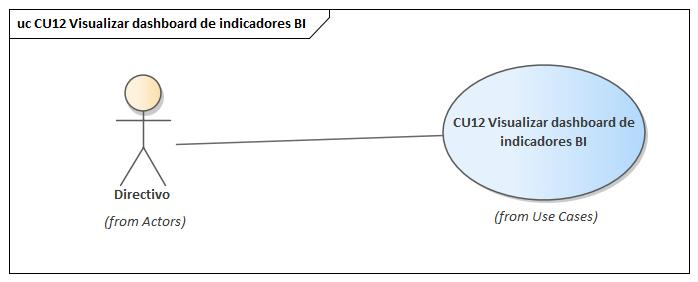
\includegraphics[width=0.8\textwidth,height=0.4\textheight,keepaspectratio]{images/071_CU12_Visualizar_Dashboard_Indicadores_BI.jpg}

\smallskip
\noindent\raggedright\textit{Nota.} Elaboración propia.
\end{figure}

\refstepcounter{table}\label{tab:detalle_cu12}
\addcontentsline{lot}{table}{\protect\numberline{\thetable}Detalle del CU-12: Visualizar dashboard de indicadores BI}
\noindent\textbf{Tabla~\thetable}\par\nopagebreak
\noindent\textit{Detalle del CU-12: Visualizar dashboard de indicadores BI}\par\nopagebreak
\begingroup\small\linespread{1}\selectfont
\begin{longtable}{>{\raggedright\arraybackslash}p{2.9cm} >{\raggedright\arraybackslash}p{12.6cm}}
\toprule
\textbf{Caso de Uso} & \textbf{CU-12. Visualizar dashboard de indicadores BI} \\
\midrule
\endfirsthead
\toprule
\textbf{Caso de Uso} & \textbf{CU-12. Visualizar dashboard de indicadores BI} \\
\midrule
\endhead
\endfoot
\bottomrule
\multicolumn{2}{l}{\textit{Nota.} Elaboración propia.} \\
\endlastfoot
\textbf{Propósito} & Brindar al Directivo un dashboard interactivo de Business Intelligence con los indicadores clave del proceso de la Beca Comedor, como apoyo a la toma de decisiones. \\
\midrule
\textbf{Descripción} & Este caso de uso describe cómo el Directivo consulta el dashboard de indicadores: postulaciones recibidas, finalistas, becas adjudicadas y asistencia promedio, con gráficos por mes de postulaciones y de asistencia, filtrados por gestión académica y, opcionalmente, por convocatoria. Los indicadores se obtienen de una vista materializada que se refresca por lotes de forma nocturna, de modo que la consulta no afecta el rendimiento de las operaciones transaccionales, y se muestra la fecha de la última actualización. El Directivo puede descargar lo que está viendo como un PDF. Es una consulta de solo lectura. Respalda el RF-07. \\
\midrule
\textbf{Actores} & Directivo. \\
\midrule
\textbf{Actor Iniciador} & Directivo. \\
\midrule
\textbf{Precondición} & \vspace{-\baselineskip}\begin{cuvin}
    \item El Directivo está autenticado en el sistema (CU-01) con el rol Directivo.
    \item Los indicadores fueron calculados en el último proceso por lotes.
\end{cuvin} \\
\midrule
\textbf{Proceso} & \textbf{Flujo principal.}
\begin{cupasos}
    \item El Directivo selecciona la opción «Dashboard de indicadores».
    \item El sistema consulta los indicadores precalculados de la gestión académica vigente, con todas sus convocatorias.
    \item El sistema muestra los cuatro indicadores (postulaciones recibidas, finalistas, becas adjudicadas y asistencia promedio), los gráficos de postulaciones y de asistencia por mes, y la fecha de su última actualización.
    \item El Directivo selecciona otra gestión académica o una convocatoria y pulsa «Aplicar».
    \item El sistema consulta los indicadores de esa selección y actualiza el dashboard.
    \item Si lo desea, el Directivo pulsa «Descargar PDF» y el sistema genera un documento con lo que está viendo y lo descarga.
\end{cupasos} \\
 & \textbf{Flujos alternativos.}
\begin{cuvin}
    \item A1 (pasos 2 y 5): si no existen datos para la gestión o la convocatoria consultada, el sistema muestra un mensaje informativo con los indicadores en cero.
    \item A2 (paso 3): si el proceso por lotes aún no se ha ejecutado, el sistema muestra los últimos indicadores disponibles con su fecha de actualización; si nunca se ejecutó, lo indica.
    \item A3 (paso 4): si la gestión o la convocatoria no existe, o la convocatoria no pertenece a la gestión, el sistema responde 404 (ERR\_DAS\_01) y conserva la última selección válida.
    \item A4 (paso 6): si no hay datos que exportar, el sistema responde 400 (ERR\_DAS\_02) y no genera el PDF.
\end{cuvin} \\
\midrule
\textbf{Postcondición} & \vspace{-\baselineskip}\begin{cuvin}
    \item El Directivo visualiza los indicadores; la consulta no modifica ningún dato del sistema.
\end{cuvin} \\
\midrule
\textbf{Excepciones} & \vspace{-\baselineskip}\begin{cuvin}
    \item Autenticación inválida o sesión expirada.
    \item Falta de permisos suficientes (el usuario no tiene el rol Directivo).
    \item Error de conexión con el servidor o la base de datos.
\end{cuvin} \\
\end{longtable}
\endgroup
\addtocounter{table}{-1}

\subsubsection{5.4.13. CU-13 Gestionar convocatoria y gestión académica}\label{sec:cap5_cu13}

\begin{figure}[H]
\caption{Diagrama de contexto del CU-13}
\label{fig:ctx_cu13}
\centering
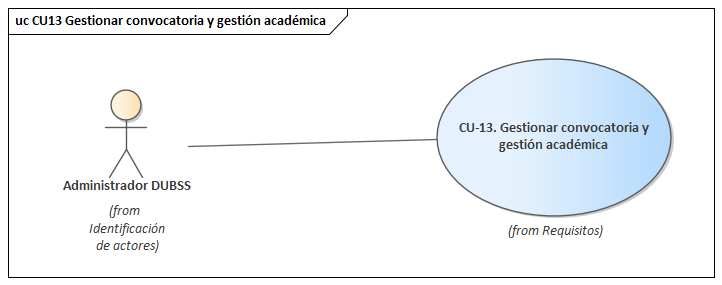
\includegraphics[width=0.8\textwidth,height=0.4\textheight,keepaspectratio]{images/042_CU13_Gestionar_Convocatoria_Gestion_Academica.png}

\smallskip
\noindent\raggedright\textit{Nota.} Elaboración propia.
\end{figure}

\refstepcounter{table}\label{tab:detalle_cu13}
\addcontentsline{lot}{table}{\protect\numberline{\thetable}Detalle del CU-13: Gestionar convocatoria y gestión académica}
\noindent\textbf{Tabla~\thetable}\par\nopagebreak
\noindent\textit{Detalle del CU-13: Gestionar convocatoria y gestión académica}\par\nopagebreak
\begingroup\small\linespread{1}\selectfont
\begin{longtable}{>{\raggedright\arraybackslash}p{2.9cm} >{\raggedright\arraybackslash}p{12.6cm}}
\toprule
\textbf{Caso de Uso} & \textbf{CU-13. Gestionar convocatoria y gestión académica} \\
\midrule
\endfirsthead
\toprule
\textbf{Caso de Uso} & \textbf{CU-13. Gestionar convocatoria y gestión académica} \\
\midrule
\endhead
\endfoot
\bottomrule
\multicolumn{2}{l}{\textit{Nota.} Elaboración propia.} \\
\endlastfoot
\textbf{Propósito} & Permitir al Administrador DUBSS crear, editar, abrir y cerrar las convocatorias de la Beca Comedor, controlando el periodo en que se reciben postulaciones. \\
\midrule
\textbf{Descripción} & Este caso de uso describe cómo el Administrador DUBSS gestiona las convocatorias y las gestiones académicas, definiendo las fechas de apertura y cierre, el número de cupos y la lista de documentos obligatorios. Solo puede recibirse una postulación (CU-02) mientras la convocatoria esté abierta, y cada postulación queda asociada a la gestión vigente. Respalda el RF-08. \\
\midrule
\textbf{Actores} & Administrador DUBSS. \\
\midrule
\textbf{Actor Iniciador} & Administrador DUBSS. \\
\midrule
\textbf{Precondición} & \vspace{-\baselineskip}\begin{cuvin}
    \item El Administrador DUBSS está autenticado en el sistema (CU-01).
    \item El Administrador cuenta con privilegios de administración.
\end{cuvin} \\
\midrule
\textbf{Proceso} & \textbf{Flujo principal.}
\begin{cupasos}
    \item El Administrador accede a la opción «Convocatorias».
    \item El sistema muestra la lista de convocatorias con su gestión académica, fechas, cupos y estado (programada, abierta o cerrada).
    \item El Administrador selecciona la acción deseada: crear, editar, abrir, cerrar o consultar una convocatoria.
    \item Para crear o editar, el Administrador ingresa la gestión académica, la fecha de apertura, la fecha de cierre, el número de cupos (por definir con la DUBSS) y la lista de documentos obligatorios (nombre, tipo y formatos permitidos).
    \item El sistema valida que la fecha de cierre sea posterior a la de apertura, que no exista otra convocatoria vigente para la misma gestión académica y que se haya definido al menos un documento obligatorio.
    \item El Administrador confirma la operación.
    \item El sistema guarda la convocatoria, actualiza su estado y registra la acción en la bitácora (CU-25).
    \item El sistema confirma la operación y muestra la lista actualizada.
\end{cupasos} \\
 & \textbf{Flujos alternativos.}
\begin{cuvin}
    \item A1 (paso 5): si ya existe una convocatoria vigente para la misma gestión académica, el sistema rechaza la operación e informa del conflicto.
    \item A2 (paso 5): si las fechas son incoherentes (cierre anterior o igual a la apertura) o hay datos obligatorios vacíos, el sistema indica los errores y permite corregirlos.
    \item A3 (paso 3): al abrir una convocatoria, el sistema cambia su estado a «abierta» y habilita el envío de postulaciones desde esa fecha.
    \item A4 (paso 3): al cerrar una convocatoria, el sistema cambia su estado a «cerrada», bloquea el envío de nuevas postulaciones y descarta o bloquea los borradores no enviados (CU-17).
    \item A5 (paso 3): si la fecha de cierre se cumple, el sistema cierra la convocatoria automáticamente.
    \item A6 (paso 4): si la convocatoria ya tiene postulaciones recibidas, el sistema restringe la edición de los documentos obligatorios y de las fechas de apertura (alcance por definir con la DUBSS) para no afectar las postulaciones existentes.
    \item A7 (paso 3): el sistema no permite eliminar una convocatoria con postulaciones asociadas; solo permite cerrarla.
\end{cuvin} \\
\midrule
\textbf{Postcondición} & \vspace{-\baselineskip}\begin{cuvin}
    \item La convocatoria queda registrada o actualizada con su gestión, fechas, cupos y documentos requeridos.
    \item El estado de la convocatoria determina si el sistema acepta o no nuevas postulaciones.
    \item La operación queda registrada en la bitácora.
\end{cuvin} \\
\midrule
\textbf{Excepciones} & \vspace{-\baselineskip}\begin{cuvin}
    \item Autenticación inválida o sesión expirada.
    \item Falta de permisos suficientes (el usuario no tiene el rol Administrador DUBSS).
    \item Datos ingresados no válidos o convocatoria duplicada para la gestión.
    \item Intento de eliminar una convocatoria con postulaciones asociadas.
    \item Error de conexión con el servidor o la base de datos.
\end{cuvin} \\
\end{longtable}
\endgroup
\addtocounter{table}{-1}

\subsubsection{5.4.14. CU-14 Gestionar usuarios y roles}\label{sec:cap5_cu14}

\begin{figure}[H]
\caption{Diagrama de contexto del CU-14}
\label{fig:ctx_cu14}
\centering
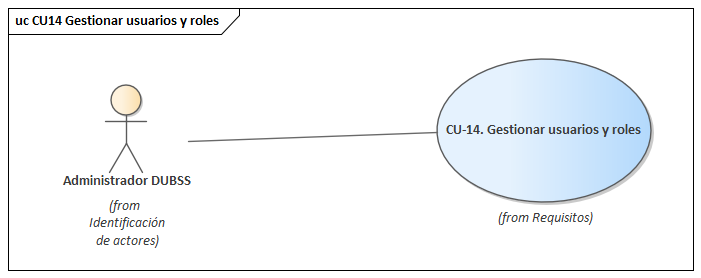
\includegraphics[width=0.8\textwidth,height=0.4\textheight,keepaspectratio]{images/043_CU14_Gestionar_Usuarios_Roles.png}

\smallskip
\noindent\raggedright\textit{Nota.} Elaboración propia.
\end{figure}

\refstepcounter{table}\label{tab:detalle_cu14}
\addcontentsline{lot}{table}{\protect\numberline{\thetable}Detalle del CU-14: Gestionar usuarios y roles}
\noindent\textbf{Tabla~\thetable}\par\nopagebreak
\noindent\textit{Detalle del CU-14: Gestionar usuarios y roles}\par\nopagebreak
\begingroup\small\linespread{1}\selectfont
\begin{longtable}{>{\raggedright\arraybackslash}p{2.9cm} >{\raggedright\arraybackslash}p{12.6cm}}
\toprule
\textbf{Caso de Uso} & \textbf{CU-14. Gestionar usuarios y roles} \\
\midrule
\endfirsthead
\toprule
\textbf{Caso de Uso} & \textbf{CU-14. Gestionar usuarios y roles} \\
\midrule
\endhead
\endfoot
\bottomrule
\multicolumn{2}{l}{\textit{Nota.} Elaboración propia.} \\
\endlastfoot
\textbf{Propósito} & Permitir al Administrador DUBSS gestionar las cuentas del personal y asignarles roles, de modo que cada persona acceda únicamente a las funciones que le corresponden. \\
\midrule
\textbf{Descripción} & Este caso de uso describe cómo el Administrador DUBSS crea, edita, desactiva y reactiva las cuentas del personal y les asigna uno de los roles del sistema (Administrador, Directivo o Personal del Comedor). Los Postulantes no se gestionan aquí, pues se registran por sí mismos (CU-01). Cada cuenta nueva recibe una contraseña temporal que se muestra una sola vez al Administrador, y cada operación (alta, edición, cambio de rol, baja y reactivación) queda en la bitácora (CU-25). Respalda el RF-09. \\
\midrule
\textbf{Actores} & Administrador DUBSS. \\
\midrule
\textbf{Actor Iniciador} & Administrador DUBSS. \\
\midrule
\textbf{Precondición} & \vspace{-\baselineskip}\begin{cuvin}
    \item El Administrador DUBSS está autenticado en el sistema (CU-01) y su cuenta está activa.
    \item El usuario autenticado tiene el rol Administrador DUBSS.
\end{cuvin} \\
\midrule
\textbf{Proceso} & \textbf{Flujo principal.}
\begin{cupasos}
    \item El Administrador accede a la opción «Usuarios y roles»; el menú ofrece una vista por rol (Administradores DUBSS, Directivos y Personal del Comedor), que es la misma lista filtrada por ese rol.
    \item El sistema muestra la lista paginada de cuentas del personal con su nombre, CI, correo, rol y estado (activa o desactivada), con filtros por rol, estado y búsqueda por CI o nombre.
    \item El Administrador selecciona la acción deseada: crear, editar, cambiar rol, desactivar o reactivar una cuenta.
    \item Para crear una cuenta, el Administrador ingresa los datos del funcionario (nombres, apellidos, CI, correo electrónico y rol).
    \item El sistema valida que los datos sean correctos, que el rol sea uno de los tres del personal y que el CI y el correo electrónico no estén registrados.
    \item El Administrador confirma la operación.
    \item El sistema crea la cuenta activa con el rol indicado y una contraseña temporal, que se muestra una sola vez al Administrador para que la entregue al funcionario (este la cambia desde su perfil, CU-15); para editar, cambiar el rol, desactivar o reactivar, actualiza la cuenta. Al cambiar el rol o desactivar, cierra las sesiones activas de esa cuenta.
    \item El sistema registra la acción (usuario, cambio realizado, fecha y hora) en la bitácora y muestra la lista actualizada.
\end{cupasos} \\
 & \textbf{Flujos alternativos.}
\begin{cuvin}
    \item A1 (paso 5): si el CI o el correo electrónico ya están registrados, el sistema rechaza el alta (409), indica el campo en conflicto y no crea la cuenta.
    \item A2 (paso 5): si faltan datos obligatorios o su formato es inválido (incluido un rol que no es del personal), el sistema responde 400, marca los errores y permite corregirlos.
    \item A3 (paso 3): si se cambia el rol de una cuenta, el sistema aplica los nuevos permisos desde su siguiente inicio de sesión y conserva el registro del cambio (rol anterior, rol nuevo, fecha y responsable).
    \item A4 (paso 3): al desactivar una cuenta, el sistema impide su acceso e invalida sus sesiones activas; la cuenta no se elimina, de modo que se preserve la trazabilidad de sus acciones.
    \item A5 (paso 3): el sistema impide que el Administrador desactive o cambie el rol de su propia cuenta o de la del último Administrador activo (403) y muestra un aviso.
    \item A6 (paso 3): el Administrador puede reactivar una cuenta desactivada, que recupera su rol anterior.
    \item A7 (paso 3): si la cuenta no existe o es la de un Postulante, el sistema responde 404; si ya está en el estado pedido (desactivar una desactivada, reactivar una activa), responde 409 e informa el estado actual.
\end{cuvin} \\
\midrule
\textbf{Postcondición} & \vspace{-\baselineskip}\begin{cuvin}
    \item La cuenta queda creada, modificada, desactivada o reactivada, y el sistema refleja el cambio de rol en los permisos del usuario.
    \item El cambio queda registrado en la bitácora.
\end{cuvin} \\
\midrule
\textbf{Excepciones} & \vspace{-\baselineskip}\begin{cuvin}
    \item Autenticación inválida o sesión expirada.
    \item Falta de permisos suficientes (el usuario no tiene el rol Administrador DUBSS).
    \item Datos ingresados no válidos o CI/correo duplicados.
    \item Error de conexión con el servidor o la base de datos.
\end{cuvin} \\
\end{longtable}
\endgroup
\addtocounter{table}{-1}

\subsubsection{5.4.15. CU-15 Recuperar contraseña / gestionar perfil}\label{sec:cap5_cu15}

\begin{figure}[H]
\caption{Diagrama de contexto del CU-15}
\label{fig:ctx_cu15}
\centering
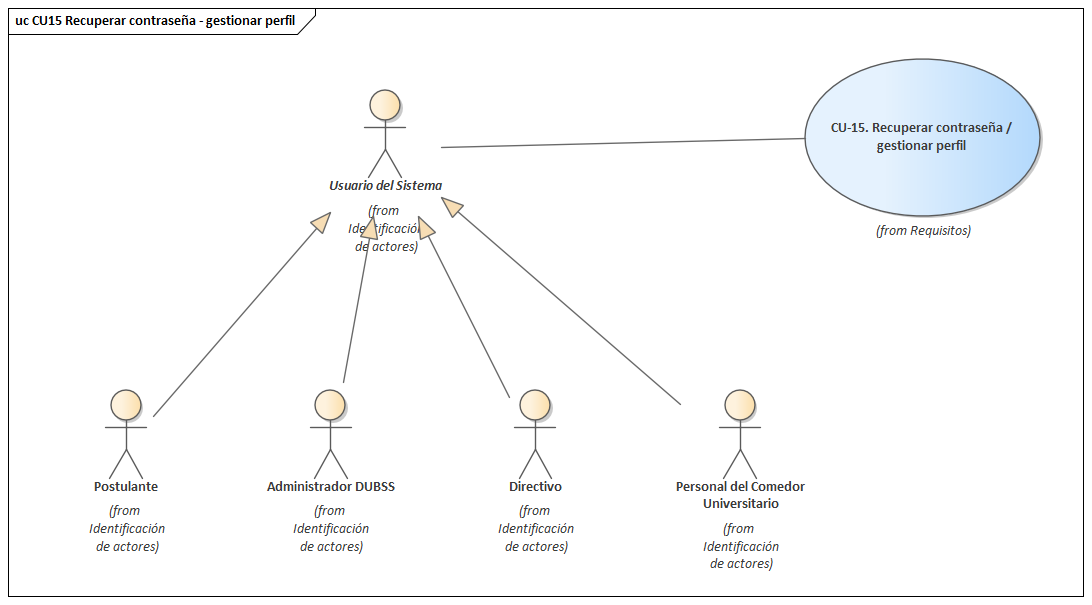
\includegraphics[width=0.8\textwidth,height=0.4\textheight,keepaspectratio]{images/044_CU15_Recuperar_Contrasena_Gestionar_Perfil.png}

\smallskip
\noindent\raggedright\textit{Nota.} Elaboración propia.
\end{figure}

\refstepcounter{table}\label{tab:detalle_cu15}
\addcontentsline{lot}{table}{\protect\numberline{\thetable}Detalle del CU-15: Recuperar contraseña / gestionar perfil}
\noindent\textbf{Tabla~\thetable}\par\nopagebreak
\noindent\textit{Detalle del CU-15: Recuperar contraseña / gestionar perfil}\par\nopagebreak
\begingroup\small\linespread{1}\selectfont
\begin{longtable}{>{\raggedright\arraybackslash}p{2.9cm} >{\raggedright\arraybackslash}p{12.6cm}}
\toprule
\textbf{Caso de Uso} & \textbf{CU-15. Recuperar contraseña / gestionar perfil} \\
\midrule
\endfirsthead
\toprule
\textbf{Caso de Uso} & \textbf{CU-15. Recuperar contraseña / gestionar perfil} \\
\midrule
\endhead
\endfoot
\bottomrule
\multicolumn{2}{l}{\textit{Nota.} Elaboración propia.} \\
\endlastfoot
\textbf{Propósito} & Permitir a los usuarios recuperar el acceso a su cuenta cuando olvidan su contraseña y mantener actualizados sus datos de contacto y su contraseña desde su perfil. \\
\midrule
\textbf{Descripción} & Este caso de uso describe dos funciones: la recuperación de contraseña mediante un enlace enviado al correo registrado (generado por el backend) y la gestión del perfil, donde el usuario autenticado actualiza sus datos de contacto y su contraseña. El CI no puede modificarse desde el perfil. Extiende al CU-01. Respalda el RF-10. \\
\midrule
\textbf{Actores} & Usuario del Sistema (Postulante, Administrador DUBSS, Directivo, Personal del Comedor Universitario); Servicio de Correo Electrónico (actor secundario, entrega el enlace). \\
\midrule
\textbf{Actor Iniciador} & Usuario del Sistema. \\
\midrule
\textbf{Precondición} & \vspace{-\baselineskip}\begin{cuvin}
    \item Recuperar contraseña: el usuario tiene una cuenta registrada con un correo electrónico al que puede acceder.
    \item Gestionar perfil: el usuario está autenticado en el sistema (CU-01).
\end{cuvin} \\
\midrule
\textbf{Proceso} & \textbf{Flujo principal A: recuperar contraseña.}
\begin{cupasos}
    \item En la pantalla de inicio de sesión, el usuario selecciona «¿Olvidó su contraseña?».
    \item El sistema solicita el correo electrónico de la cuenta.
    \item El usuario ingresa su correo y confirma la solicitud.
    \item El sistema genera un token de restablecimiento de un solo uso con tiempo de validez limitado, lo envía en un enlace al correo registrado y muestra un mensaje informando que, si el correo está registrado, recibirá las instrucciones.
    \item El usuario abre el enlace recibido y define una nueva contraseña que cumpla la política de seguridad.
    \item El sistema guarda la nueva contraseña, invalida el enlace, desbloquea la cuenta si estaba bloqueada, cierra todas las sesiones abiertas de la cuenta y permite al usuario iniciar sesión con la nueva contraseña.
\end{cupasos} \\
 & \textbf{Flujo principal B: gestionar perfil.}
\begin{cupasos}
    \item El usuario autenticado accede a la opción «Mi perfil».
    \item El sistema muestra sus datos personales y de contacto; el CI se muestra solo de lectura.
    \item El usuario modifica sus datos de contacto (el correo electrónico y, si es Postulante, el teléfono) y/o solicita cambiar su contraseña ingresando la contraseña actual y la nueva.
    \item El sistema valida los datos, comprueba la unicidad del correo y la política de contraseña.
    \item El sistema guarda los cambios, registra la acción en la bitácora y confirma la actualización; si cambió la contraseña, cierra las sesiones de los demás dispositivos y mantiene la actual.
\end{cupasos} \\
 & \textbf{Flujos alternativos.}
\begin{cuvin}
    \item A1 (flujo A, paso 4): si el correo no está registrado, el sistema muestra el mismo mensaje neutro, para no revelar qué correos existen en el sistema.
    \item A2 (flujo A, paso 5): si el enlace expiró o ya fue utilizado, el sistema informa del hecho y permite solicitar uno nuevo.
    \item A3 (flujo A, paso 5): si la nueva contraseña no cumple la política de seguridad, el sistema muestra los requisitos y permite reintentar.
    \item A4 (flujo B, paso 3): si el usuario intenta modificar su CI, el sistema no lo permite (campo bloqueado).
    \item A5 (flujo B, paso 4): si el nuevo correo electrónico ya pertenece a otra cuenta, el sistema rechaza el cambio.
    \item A6 (flujo B, paso 4): si la contraseña actual ingresada es incorrecta, el sistema rechaza el cambio de contraseña.
    \item A7 (flujo B, paso 5): si se cambia el correo electrónico, el sistema exige la contraseña actual (reautenticación) antes de guardarlo.
\end{cuvin} \\
\midrule
\textbf{Postcondición} & \vspace{-\baselineskip}\begin{cuvin}
    \item Recuperar contraseña: la cuenta queda con una nueva contraseña y el usuario puede autenticarse.
    \item Gestionar perfil: los datos de contacto y/o la contraseña quedan actualizados y se utilizarán en las notificaciones al usuario.
\end{cuvin} \\
\midrule
\textbf{Excepciones} & \vspace{-\baselineskip}\begin{cuvin}
    \item Autenticación inválida o sesión expirada (en la gestión de perfil).
    \item Datos ingresados no válidos.
    \item Enlace de restablecimiento inválido o expirado.
    \item Servicio de envío de correo electrónico no disponible.
    \item Error de conexión con el servidor o la base de datos.
\end{cuvin} \\
\end{longtable}
\endgroup
\addtocounter{table}{-1}

\subsubsection{5.4.16. CU-16 Digitalizar y adjuntar documentos}\label{sec:cap5_cu16}

\begin{figure}[H]
\caption{Diagrama de contexto del CU-16}
\label{fig:ctx_cu16}
\centering
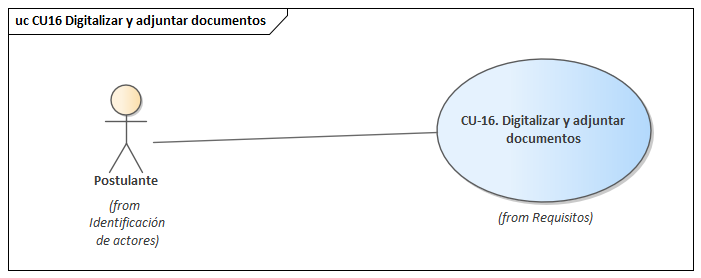
\includegraphics[width=0.8\textwidth,height=0.4\textheight,keepaspectratio]{images/045_CU16_Digitalizar_Adjuntar_Documentos.png}

\smallskip
\noindent\raggedright\textit{Nota.} Elaboración propia.
\end{figure}

\refstepcounter{table}\label{tab:detalle_cu16}
\addcontentsline{lot}{table}{\protect\numberline{\thetable}Detalle del CU-16: Digitalizar y adjuntar documentos}
\noindent\textbf{Tabla~\thetable}\par\nopagebreak
\noindent\textit{Detalle del CU-16: Digitalizar y adjuntar documentos}\par\nopagebreak
\begingroup\small\linespread{1}\selectfont
\begin{longtable}{>{\raggedright\arraybackslash}p{2.9cm} >{\raggedright\arraybackslash}p{12.6cm}}
\toprule
\textbf{Caso de Uso} & \textbf{CU-16. Digitalizar y adjuntar documentos} \\
\midrule
\endfirsthead
\toprule
\textbf{Caso de Uso} & \textbf{CU-16. Digitalizar y adjuntar documentos} \\
\midrule
\endhead
\endfoot
\bottomrule
\multicolumn{2}{l}{\textit{Nota.} Elaboración propia.} \\
\endlastfoot
\textbf{Propósito} & Permitir al Postulante digitalizar sus documentos con la cámara del teléfono, o cargarlos desde un archivo en la web, y asociarlos a su postulación como respaldo de los datos declarados. \\
\midrule
\textbf{Descripción} & Este caso de uso describe cómo el Postulante captura o adjunta cada documento requerido por la convocatoria, valida su formato y tamaño, revisa una vista previa y lo asocia a su postulación, almacenándolo en MinIO. Es incluido por el CU-02 y también se utiliza al completar un borrador (CU-17). Permite evitar la presentación de carpetas físicas en la etapa inicial. Respalda el RF-11. \\
\midrule
\textbf{Actores} & Postulante. \\
\midrule
\textbf{Actor Iniciador} & Postulante. \\
\midrule
\textbf{Precondición} & \vspace{-\baselineskip}\begin{cuvin}
    \item El Postulante está autenticado en el sistema (CU-01).
    \item El Postulante se encuentra completando una postulación o un borrador, con la convocatoria abierta.
    \item La convocatoria tiene definida la lista de documentos requeridos.
    \item En la aplicación móvil, el Postulante otorgó el permiso de uso de la cámara.
\end{cuvin} \\
\midrule
\textbf{Proceso} & \textbf{Flujo principal.}
\begin{cupasos}
    \item El sistema muestra la lista de documentos requeridos por la convocatoria, indicando cuáles están pendientes y cuáles ya fueron adjuntados.
    \item El Postulante selecciona el documento que desea adjuntar.
    \item En la aplicación móvil, el Postulante captura el documento con la cámara del dispositivo; en el portal web, selecciona un archivo de su equipo.
    \item El sistema valida el formato y el tamaño del archivo (formatos y tamaño máximo por definir con la DUBSS).
    \item El sistema muestra una vista previa del documento.
    \item El Postulante confirma el documento, o bien lo reemplaza, lo vuelve a capturar o lo elimina.
    \item El sistema almacena el archivo en MinIO y registra el documento adjunto (tipo y archivo) asociado a la postulación.
    \item El sistema actualiza la lista de documentos con el estado «adjuntado».
\end{cupasos} \\
 & \textbf{Flujos alternativos.}
\begin{cuvin}
    \item A1 (paso 3): si el Postulante no otorga el permiso de la cámara, el sistema le ofrece seleccionar el documento desde la galería o los archivos del dispositivo.
    \item A2 (paso 4): si el formato no es permitido o el tamaño excede el máximo, el sistema rechaza el archivo y muestra un mensaje de error.
    \item A3 (paso 6): el Postulante puede reemplazar o eliminar un documento ya adjuntado, siempre que la postulación no haya sido enviada o se encuentre devuelta (CU-19).
    \item A4 (paso 7): si falla la carga por problemas de conexión, el sistema permite reintentar sin perder los demás documentos ya adjuntados.
    \item A5 (paso 3): el Postulante puede adjuntar más de un archivo o página para un mismo documento (cantidad máxima por definir).
    \item A6 (general): si al enviar la postulación faltan documentos obligatorios, el CU-02 no permite el envío e indica los documentos faltantes.
\end{cuvin} \\
\midrule
\textbf{Postcondición} & \vspace{-\baselineskip}\begin{cuvin}
    \item Los documentos adjuntados quedan almacenados en MinIO y vinculados a la postulación (o al borrador).
    \item La lista de documentos requeridos refleja cuáles fueron cargados y cuáles faltan.
\end{cuvin} \\
\midrule
\textbf{Excepciones} & \vspace{-\baselineskip}\begin{cuvin}
    \item Autenticación inválida o sesión expirada.
    \item Permiso de cámara denegado.
    \item Formato o tamaño de archivo no permitido.
    \item Error al almacenar el archivo en MinIO.
    \item Convocatoria cerrada durante la carga de documentos.
    \item Error de conexión con el servidor.
\end{cuvin} \\
\end{longtable}
\endgroup
\addtocounter{table}{-1}

\subsubsection{5.4.17. CU-17 Guardar borrador de postulación}\label{sec:cap5_cu17}

\begin{figure}[H]
\caption{Diagrama de contexto del CU-17}
\label{fig:ctx_cu17}
\centering
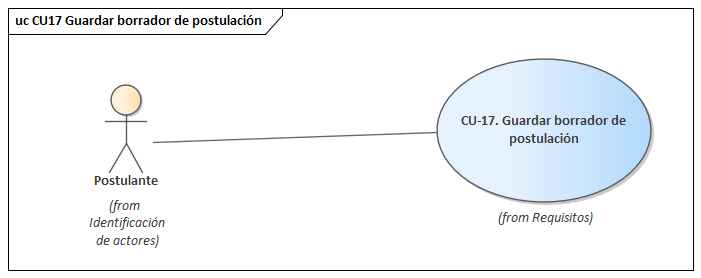
\includegraphics[width=0.8\textwidth,height=0.4\textheight,keepaspectratio]{images/046_CU17_Guardar_Borrador_Postulacion.png}

\smallskip
\noindent\raggedright\textit{Nota.} Elaboración propia.
\end{figure}

\refstepcounter{table}\label{tab:detalle_cu17}
\addcontentsline{lot}{table}{\protect\numberline{\thetable}Detalle del CU-17: Guardar borrador de postulación}
\noindent\textbf{Tabla~\thetable}\par\nopagebreak
\noindent\textit{Detalle del CU-17: Guardar borrador de postulación}\par\nopagebreak
\begingroup\small\linespread{1}\selectfont
\begin{longtable}{>{\raggedright\arraybackslash}p{2.9cm} >{\raggedright\arraybackslash}p{12.6cm}}
\toprule
\textbf{Caso de Uso} & \textbf{CU-17. Guardar borrador de postulación} \\
\midrule
\endfirsthead
\toprule
\textbf{Caso de Uso} & \textbf{CU-17. Guardar borrador de postulación} \\
\midrule
\endhead
\endfoot
\bottomrule
\multicolumn{2}{l}{\textit{Nota.} Elaboración propia.} \\
\endlastfoot
\textbf{Propósito} & Permitir al Postulante guardar su postulación incompleta como borrador y retomarla posteriormente sin perder lo ya ingresado. \\
\midrule
\textbf{Descripción} & Este caso de uso describe cómo el Postulante guarda el avance del formulario socioeconómico y de los documentos adjuntos, sin necesidad de completar los campos obligatorios, y cómo lo retoma después para completarlo y enviarlo. Un borrador no es una postulación enviada, por lo que no se procesa con el módulo de IA ni cuenta como postulación vigente. Extiende al CU-02. Respalda el RF-12. \\
\midrule
\textbf{Actores} & Postulante. \\
\midrule
\textbf{Actor Iniciador} & Postulante. \\
\midrule
\textbf{Precondición} & \vspace{-\baselineskip}\begin{cuvin}
    \item El Postulante está autenticado en el sistema (CU-01).
    \item Existe una convocatoria abierta (CU-13).
    \item El Postulante no tiene una postulación vigente ya enviada en la misma gestión.
\end{cuvin} \\
\midrule
\textbf{Proceso} & \textbf{Flujo principal A: guardar borrador.}
\begin{cupasos}
    \item Durante el llenado del formulario (CU-02), el Postulante selecciona «Guardar borrador».
    \item El sistema verifica que la convocatoria continúe abierta.
    \item El sistema guarda los datos ingresados hasta ese momento y las referencias a los documentos ya adjuntados, sin exigir los campos ni documentos obligatorios.
    \item El sistema registra la fecha y hora del último guardado.
    \item El sistema confirma que el borrador fue guardado.
\end{cupasos} \\
 & \textbf{Flujo principal B: retomar borrador.}
\begin{cupasos}
    \item El Postulante accede a la opción «Mi borrador» o «Nueva postulación».
    \item El sistema detecta el borrador y lo muestra con los datos y documentos previamente guardados.
    \item El Postulante continúa completando el formulario y puede guardar el borrador nuevamente o enviar la postulación (CU-02).
\end{cupasos} \\
 & \textbf{Flujos alternativos.}
\begin{cuvin}
    \item A1 (flujo A, paso 2): si la convocatoria ya está cerrada, el sistema no permite guardar ni editar el borrador e informa que el plazo finalizó.
    \item A2 (flujo A, paso 3): si algún campo contiene un valor con formato inválido (por ejemplo, texto en un campo numérico), el sistema lo señala y no guarda ese valor.
    \item A3 (flujo A, paso 3): si falla la conexión, el sistema informa que no se guardó el borrador y permite reintentar.
    \item A4 (flujo B, paso 2): si no existe un borrador, el sistema inicia una postulación nueva.
    \item A5 (flujo B, paso 3): al enviarse la postulación, el borrador se convierte en postulación y deja de existir como borrador.
    \item A6 (general): al cerrar la convocatoria, el sistema descarta o bloquea los borradores no enviados (CU-13).
\end{cuvin} \\
\midrule
\textbf{Postcondición} & \vspace{-\baselineskip}\begin{cuvin}
    \item El borrador queda guardado con su fecha de último guardado y puede retomarse mientras la convocatoria esté abierta.
    \item El borrador no se considera enviado, no se procesa con el módulo de IA y no modifica el estado de ninguna postulación.
\end{cuvin} \\
\midrule
\textbf{Excepciones} & \vspace{-\baselineskip}\begin{cuvin}
    \item Autenticación inválida o sesión expirada.
    \item Convocatoria cerrada.
    \item Datos con formato inválido.
    \item Error de conexión con el servidor o la base de datos.
\end{cuvin} \\
\end{longtable}
\endgroup
\addtocounter{table}{-1}

\subsubsection{5.4.18. CU-18 Validar elegibilidad y duplicados}\label{sec:cap5_cu18}

\begin{figure}[H]
\caption{Diagrama de contexto del CU-18}
\label{fig:ctx_cu18}
\centering
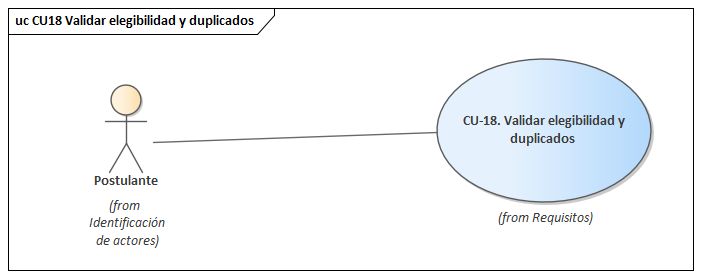
\includegraphics[width=0.8\textwidth,height=0.4\textheight,keepaspectratio]{images/047_CU18_Validar_Elegibilidad_Duplicados.png}

\smallskip
\noindent\raggedright\textit{Nota.} Elaboración propia.
\end{figure}

\refstepcounter{table}\label{tab:detalle_cu18}
\addcontentsline{lot}{table}{\protect\numberline{\thetable}Detalle del CU-18: Validar elegibilidad y duplicados}
\noindent\textbf{Tabla~\thetable}\par\nopagebreak
\noindent\textit{Detalle del CU-18: Validar elegibilidad y duplicados}\par\nopagebreak
\begingroup\small\linespread{1}\selectfont
\begin{longtable}{>{\raggedright\arraybackslash}p{2.9cm} >{\raggedright\arraybackslash}p{12.6cm}}
\toprule
\textbf{Caso de Uso} & \textbf{CU-18. Validar elegibilidad y duplicados} \\
\midrule
\endfirsthead
\toprule
\textbf{Caso de Uso} & \textbf{CU-18. Validar elegibilidad y duplicados} \\
\midrule
\endhead
\endfoot
\bottomrule
\multicolumn{2}{l}{\textit{Nota.} Elaboración propia.} \\
\endlastfoot
\textbf{Propósito} & Verificar, al momento de recibir una postulación, que el postulante cumple las condiciones de elegibilidad y que no existe otra postulación vigente suya en la misma gestión. \\
\midrule
\textbf{Descripción} & Este caso de uso describe la validación automática que ejecuta el sistema cuando el Postulante envía su postulación: comprueba las condiciones de elegibilidad definidas por la DUBSS y la unicidad de la postulación por postulante y gestión. Evita registros duplicados o inválidos que distorsionen la priorización y la adjudicación. Es incluido por el CU-02. Respalda el RF-13. \\
\midrule
\textbf{Actores} & Postulante. \\
\midrule
\textbf{Actor Iniciador} & Postulante (a través del CU-02, al enviar su postulación; el sistema ejecuta la validación). \\
\midrule
\textbf{Precondición} & \vspace{-\baselineskip}\begin{cuvin}
    \item El Postulante envió su postulación con los campos y documentos obligatorios completos (CU-02).
    \item Existe una convocatoria abierta a la que se asocia la postulación.
    \item Las condiciones de elegibilidad están configuradas en el sistema (por definir con la DUBSS).
\end{cuvin} \\
\midrule
\textbf{Proceso} & \textbf{Flujo principal.}
\begin{cupasos}
    \item El sistema recibe la solicitud de validación con la identidad del Postulante y la convocatoria de destino.
    \item El sistema consulta las postulaciones existentes del Postulante en la misma gestión académica.
    \item El sistema verifica que no exista otra postulación vigente del Postulante en la convocatoria.
    \item El sistema verifica las condiciones de elegibilidad (por ejemplo, la condición de estudiante de la UAGRM según su CI y perfil; reglas por definir con la DUBSS).
    \item El sistema devuelve al CU-02 el resultado «válida».
    \item El CU-02 continúa con el registro de la postulación.
\end{cupasos} \\
 & \textbf{Flujos alternativos.}
\begin{cuvin}
    \item A1 (paso 3): si ya existe otra postulación vigente del Postulante en la gestión, el sistema devuelve el resultado «duplicada» y el CU-02 rechaza el envío e informa el motivo.
    \item A2 (paso 4): si el Postulante no cumple alguna condición de elegibilidad, el sistema devuelve el resultado «no elegible» con el motivo específico, y el CU-02 rechaza el envío.
    \item A3 (paso 3): si se trata del reenvío de una postulación devuelta (CU-19), el sistema no la considera duplicada y la vincula con la postulación original, conservando el historial.
    \item A4 (paso 3): si se recibe una solicitud duplicada, el sistema devuelve el mismo resultado sin generar registros adicionales (idempotencia).
    \item A5 (paso 2): si el servicio de validación no está disponible, el sistema no acepta la postulación e informa al Postulante que reintente.
\end{cuvin} \\
\midrule
\textbf{Postcondición} & \vspace{-\baselineskip}\begin{cuvin}
    \item El sistema determina si la postulación es válida y, en caso afirmativo, el CU-02 puede registrarla.
    \item Si la postulación es rechazada, no se crea ningún registro y el Postulante recibe el motivo del rechazo.
\end{cuvin} \\
\midrule
\textbf{Excepciones} & \vspace{-\baselineskip}\begin{cuvin}
    \item Postulación duplicada en la misma gestión.
    \item Postulante no elegible según las condiciones establecidas.
    \item Servicio de validación no disponible.
    \item Error de conexión con el servidor o la base de datos.
\end{cuvin} \\
\end{longtable}
\endgroup
\addtocounter{table}{-1}

\subsubsection{5.4.19. CU-19 Devolver postulación para corrección}\label{sec:cap5_cu19}

\begin{figure}[H]
\caption{Diagrama de contexto del CU-19}
\label{fig:ctx_cu19}
\centering
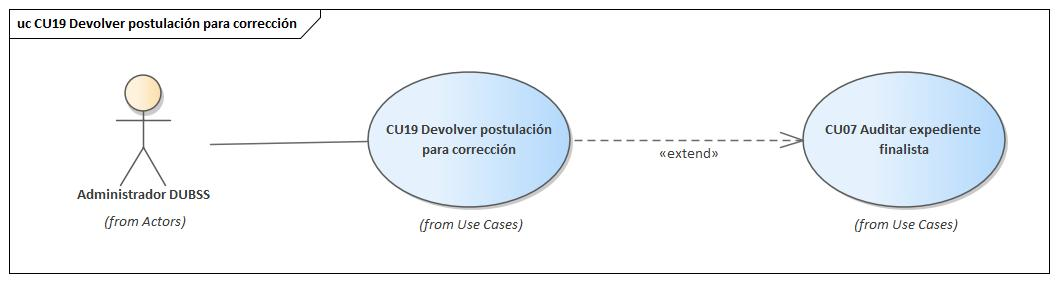
\includegraphics[width=0.8\textwidth,height=0.4\textheight,keepaspectratio]{images/072_CU19_Devolver_Postulacion_Correccion.jpg}

\smallskip
\noindent\raggedright\textit{Nota.} Elaboración propia.
\end{figure}

\refstepcounter{table}\label{tab:detalle_cu19}
\addcontentsline{lot}{table}{\protect\numberline{\thetable}Detalle del CU-19: Devolver postulación para corrección}
\noindent\textbf{Tabla~\thetable}\par\nopagebreak
\noindent\textit{Detalle del CU-19: Devolver postulación para corrección}\par\nopagebreak
\begingroup\small\linespread{1}\selectfont
\begin{longtable}{>{\raggedright\arraybackslash}p{2.9cm} >{\raggedright\arraybackslash}p{12.6cm}}
\toprule
\textbf{Caso de Uso} & \textbf{CU-19. Devolver postulación para corrección} \\
\midrule
\endfirsthead
\toprule
\textbf{Caso de Uso} & \textbf{CU-19. Devolver postulación para corrección} \\
\midrule
\endhead
\endfoot
\bottomrule
\multicolumn{2}{l}{\textit{Nota.} Elaboración propia.} \\
\endlastfoot
\textbf{Propósito} & Permitir al Administrador DUBSS devolver una postulación con observaciones para que el Postulante corrija o complete su documentación y la reenvíe, evitando descartarla por defectos subsanables. \\
\midrule
\textbf{Descripción} & Este caso de uso describe cómo el Administrador DUBSS, durante la auditoría de un expediente finalista, devuelve la postulación al Postulante desde el expediente del finalista, registrando un motivo de hasta 500 caracteres con las observaciones que debe subsanar. La postulación cambia al estado «devuelta», el cambio queda en el historial de la postulación y en la bitácora, y el Postulante recibe siempre el aviso por bandeja, push y correo. No hay plazo de reenvío ni límite de devoluciones: el Postulante puede corregir y reenviar la postulación cuando quiera mediante el CU-02. Extiende el CU-07. Respalda el RF-14. \\
\midrule
\textbf{Actores} & Administrador DUBSS. \\
\midrule
\textbf{Actor Iniciador} & Administrador DUBSS. \\
\midrule
\textbf{Precondición} & \vspace{-\baselineskip}\begin{cuvin}
    \item El Administrador DUBSS está autenticado en el sistema (CU-01) con el rol Administrador DUBSS.
    \item El Administrador DUBSS se encuentra auditando el expediente de un finalista (CU-07).
    \item La postulación se encuentra en estado «calificada».
    \item El finalista tiene al menos una auditoría registrada después de su última devolución; no se exige entrega física.
\end{cuvin} \\
\midrule
\textbf{Proceso} & \textbf{Flujo principal.}
\begin{cupasos}
    \item El Administrador DUBSS selecciona la opción «Devolver para corrección» en el expediente.
    \item El sistema solicita el motivo de la devolución (máximo 500 caracteres).
    \item El Administrador DUBSS registra el motivo y confirma la devolución.
    \item El sistema valida que el motivo no esté vacío ni supere los 500 caracteres, que la postulación siga en estado «calificada» y que exista una auditoría posterior a la última devolución.
    \item El sistema actualiza el estado de la postulación a «devuelta».
    \item El sistema registra, en una sola operación, el cambio en el historial de la postulación (estado anterior, estado nuevo, usuario y motivo) y en la bitácora.
    \item El sistema crea la notificación para el Postulante y se la envía siempre por bandeja, push y correo, con las observaciones.
    \item El sistema confirma la devolución al Administrador DUBSS.
\end{cupasos} \\
 & \textbf{Flujos alternativos.}
\begin{cuvin}
    \item A1 (paso 4): si el motivo está vacío o supera los 500 caracteres, el sistema no permite devolver la postulación.
    \item A5 (paso 4): si el finalista no existe, el sistema informa que no se encontró.
    \item A6 (paso 4): si la postulación ya no está «calificada» (incluye a dos administradores actuando a la vez), el sistema rechaza la devolución por conflicto de estado.
    \item A7 (paso 4): si no hay una auditoría registrada después de la última devolución, el sistema rechaza la devolución por conflicto.
    \item A8 (paso 5): si la petición se repite por doble clic, la segunda se rechaza por estado inválido; el botón se deshabilita al enviar.
    \item A2 (paso 3): si el Administrador DUBSS cancela la operación, la postulación conserva su estado.
    \item A3 (paso 7): si falla el envío del push, la notificación queda en la bandeja del Postulante y el servicio de notificaciones la reintenta; el Postulante también puede verla al consultar su postulación (CU-04).
    \item A4 (posterior al paso 8): el reenvío es del CU-02; cuando el Postulante corrige y reenvía la postulación, esta vuelve al estado «pendiente», se incrementa su número de envíos, se conserva el historial de devoluciones y reenvíos, y sigue el mismo flujo del CU-07 (nueva entrega física si hace falta y nueva auditoría; las anteriores se conservan).
\end{cuvin} \\
\midrule
\textbf{Postcondición} & \vspace{-\baselineskip}\begin{cuvin}
    \item La postulación queda en estado «devuelta» con las observaciones registradas en su historial.
    \item El Postulante es notificado y puede consultar las observaciones (CU-04).
\end{cuvin} \\
\midrule
\textbf{Excepciones} & \vspace{-\baselineskip}\begin{cuvin}
    \item Autenticación inválida o sesión expirada.
    \item Falta de permisos suficientes (el usuario no tiene el rol Administrador DUBSS).
    \item La postulación no se encuentra en un estado que permita su devolución (conflicto de estado).
    \item El finalista indicado no existe.
    \item Error al enviar la notificación push mediante Firebase Cloud Messaging.
    \item Error de conexión con el servidor o la base de datos.
\end{cuvin} \\
\end{longtable}
\endgroup
\addtocounter{table}{-1}

\subsubsection{5.4.20. CU-20 Archivar o rechazar postulación}\label{sec:cap5_cu20}

\begin{figure}[H]
\caption{Diagrama de contexto del CU-20}
\label{fig:ctx_cu20}
\centering
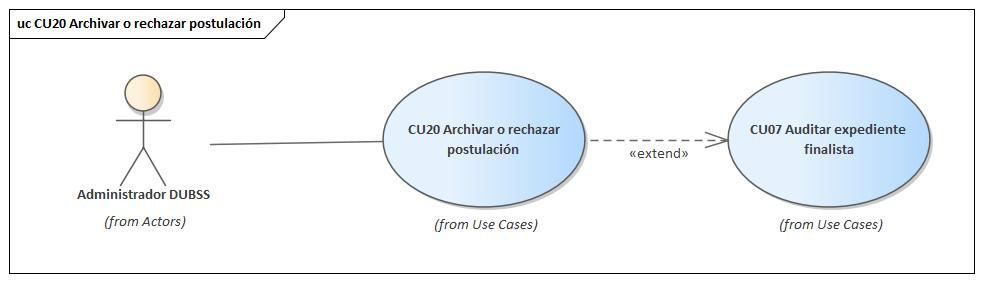
\includegraphics[width=0.8\textwidth,height=0.4\textheight,keepaspectratio]{images/073_CU20_Archivar_Rechazar_Postulacion.jpg}

\smallskip
\noindent\raggedright\textit{Nota.} Elaboración propia.
\end{figure}

\refstepcounter{table}\label{tab:detalle_cu20}
\addcontentsline{lot}{table}{\protect\numberline{\thetable}Detalle del CU-20: Archivar o rechazar postulación}
\noindent\textbf{Tabla~\thetable}\par\nopagebreak
\noindent\textit{Detalle del CU-20: Archivar o rechazar postulación}\par\nopagebreak
\begingroup\small\linespread{1}\selectfont
\begin{longtable}{>{\raggedright\arraybackslash}p{2.9cm} >{\raggedright\arraybackslash}p{12.6cm}}
\toprule
\textbf{Caso de Uso} & \textbf{CU-20. Archivar o rechazar postulación} \\
\midrule
\endfirsthead
\toprule
\textbf{Caso de Uso} & \textbf{CU-20. Archivar o rechazar postulación} \\
\midrule
\endhead
\endfoot
\bottomrule
\multicolumn{2}{l}{\textit{Nota.} Elaboración propia.} \\
\endlastfoot
\textbf{Propósito} & Permitir al Administrador DUBSS cerrar formalmente una postulación que no procede, archivándola o rechazándola, y dejar constancia del motivo de la decisión. \\
\midrule
\textbf{Descripción} & Este caso de uso describe cómo el Administrador DUBSS, durante la auditoría de un expediente finalista, archiva o rechaza una postulación registrando el motivo. Al archivarla, la postulación pasa al estado «archivada»; al rechazarla, pasa al estado «no adjudicada». En ambos casos deja de aparecer en la lista priorizada activa, el cambio queda en el historial de la postulación y esta se conserva para consulta histórica y reportes. Extiende el CU-07. Respalda el RF-15. \\
\midrule
\textbf{Actores} & Administrador DUBSS. \\
\midrule
\textbf{Actor Iniciador} & Administrador DUBSS. \\
\midrule
\textbf{Precondición} & \vspace{-\baselineskip}\begin{cuvin}
    \item El Administrador DUBSS está autenticado en el sistema (CU-01) con el rol Administrador DUBSS.
    \item El Administrador DUBSS se encuentra auditando el expediente de un finalista (CU-07).
    \item La postulación se encuentra en estado «calificada».
\end{cuvin} \\
\midrule
\textbf{Proceso} & \textbf{Flujo principal A: archivar la postulación.}
\begin{cupasos}
    \item El Administrador DUBSS selecciona la opción «Archivar» en el expediente.
    \item El sistema solicita el motivo del archivo.
    \item El Administrador DUBSS registra el motivo y confirma.
    \item El sistema valida que el motivo no esté vacío.
    \item El sistema actualiza el estado de la postulación a «archivada» y la retira de la lista priorizada activa.
    \item El sistema registra el cambio en el historial de la postulación (estado anterior, estado nuevo, usuario y motivo) y en la bitácora, y confirma la operación.
\end{cupasos} \\
 & \textbf{Flujo principal B: rechazar la postulación.}
\begin{cupasos}
    \item El Administrador DUBSS selecciona la opción «Rechazar» en el expediente.
    \item El sistema solicita el motivo del rechazo.
    \item El Administrador DUBSS registra el motivo y confirma.
    \item El sistema valida que el motivo no esté vacío.
    \item El sistema actualiza el estado de la postulación a «no adjudicada» y la retira de la lista priorizada activa.
    \item El sistema registra el cambio en el historial de la postulación (estado anterior, estado nuevo, usuario y motivo) y en la bitácora, y confirma la operación.
\end{cupasos} \\
 & \textbf{Flujos alternativos.}
\begin{cuvin}
    \item A1 (flujos A y B, paso 4): si no se registra el motivo, el sistema no permite completar la operación.
    \item A2 (flujos A y B, paso 3): si el Administrador DUBSS cancela la operación, la postulación conserva su estado.
    \item A3 (flujos A y B, paso 1): si la postulación ya se encuentra en un estado final («archivada», «adjudicada» o «no adjudicada») o los resultados de la convocatoria fueron publicados (CU-22), el sistema no permite la operación.
\end{cuvin} \\
\midrule
\textbf{Postcondición} & \vspace{-\baselineskip}\begin{cuvin}
    \item La postulación queda en estado «archivada» o «no adjudicada», con el motivo registrado en su historial, y se conserva para consulta histórica y reportes.
    \item El Postulante puede consultar el estado y el motivo registrado (CU-04).
\end{cuvin} \\
\midrule
\textbf{Excepciones} & \vspace{-\baselineskip}\begin{cuvin}
    \item Autenticación inválida o sesión expirada.
    \item Falta de permisos suficientes (el usuario no tiene el rol Administrador DUBSS).
    \item La postulación no se encuentra en un estado que permita archivarla o rechazarla.
    \item Error de conexión con el servidor o la base de datos.
\end{cuvin} \\
\end{longtable}
\endgroup
\addtocounter{table}{-1}

\subsubsection{5.4.21. CU-21 Notificar finalistas, registrar entrega de documentación física y publicar comunicados/avisos}\label{sec:cap5_cu21}

\begin{figure}[H]
\caption{Diagrama de contexto del CU-21}
\label{fig:ctx_cu21}
\centering
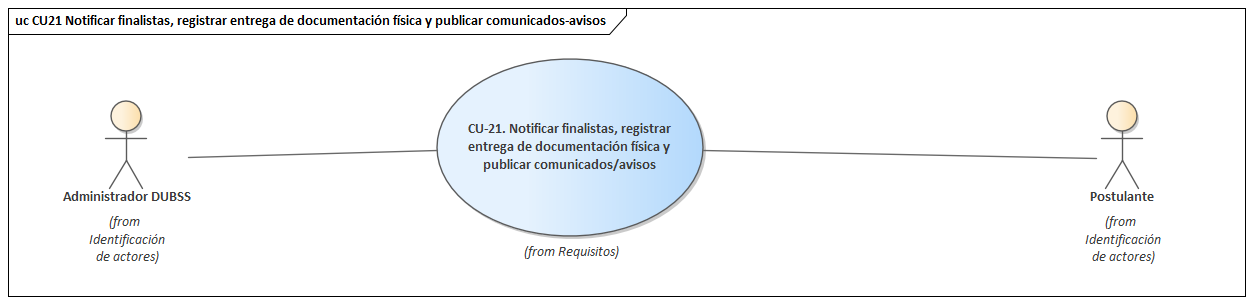
\includegraphics[width=0.8\textwidth,height=0.4\textheight,keepaspectratio]{images/048_CU21_Notificar_Finalistas_Publicar_Avisos.png}

\smallskip
\noindent\raggedright\textit{Nota.} Elaboración propia.
\end{figure}

\refstepcounter{table}\label{tab:detalle_cu21}
\addcontentsline{lot}{table}{\protect\numberline{\thetable}Detalle del CU-21: Notificar finalistas, registrar entrega de documentación física y publicar comunicados/avisos}
\noindent\textbf{Tabla~\thetable}\par\nopagebreak
\noindent\textit{Detalle del CU-21: Notificar finalistas, registrar entrega de documentación física y publicar comunicados/avisos}\par\nopagebreak
\begingroup\small\linespread{1}\selectfont
\begin{longtable}{>{\raggedright\arraybackslash}p{2.9cm} >{\raggedright\arraybackslash}p{12.6cm}}
\toprule
\textbf{Caso de Uso} & \textbf{CU-21. Notificar finalistas, registrar entrega de documentación física y publicar comunicados/avisos} \\
\midrule
\endfirsthead
\toprule
\textbf{Caso de Uso} & \textbf{CU-21. Notificar finalistas, registrar entrega de documentación física y publicar comunicados/avisos} \\
\midrule
\endhead
\endfoot
\bottomrule
\multicolumn{2}{l}{\textit{Nota.} Elaboración propia.} \\
\endlastfoot
\textbf{Propósito} & Permitir al Administrador DUBSS notificar a los finalistas para que presenten su documentación física, registrar su recepción y publicar comunicados y avisos dirigidos a los postulantes. \\
\midrule
\textbf{Descripción} & Este caso de uso agrupa tres funciones que coordinan la auditoría física: notificar a los finalistas el plazo y los documentos que deben presentar, registrar la fecha en que se recibe la documentación física de cada uno y publicar comunicados o avisos generales. Cada aviso a un finalista se guarda en su bandeja y se envía por notificación push (Firebase Cloud Messaging) y por correo; los comunicados llegan a la bandeja y por push, y el postulante los consulta en la web o en la aplicación. La pantalla de finalistas muestra además la última auditoría de cada uno, la insignia «Devuelta» cuando la postulación fue devuelta y la acción «Auditar» (CU-07); todo aviso se envía por el servicio de notificaciones. Es incluido por el CU-07 (Auditar expediente finalista). Respalda el RF-16. \\
\midrule
\textbf{Actores} & Administrador DUBSS; Postulante (receptor de las notificaciones). \\
\midrule
\textbf{Actor Iniciador} & Administrador DUBSS. \\
\midrule
\textbf{Precondición} & \vspace{-\baselineskip}\begin{cuvin}
    \item El Administrador DUBSS está autenticado en el sistema (CU-01) con el rol Administrador DUBSS y su cuenta está activa.
    \item Para notificar finalistas y registrar entregas: la convocatoria tiene finalistas seleccionados (CU-05), en el marco de la auditoría (CU-07).
    \item Para publicar comunicados: existe al menos un grupo de destinatarios (todos los postulantes o los finalistas).
\end{cuvin} \\
\midrule
\textbf{Proceso} & \textbf{Flujo principal A: notificar a los finalistas.}
\begin{cupasos}
    \item El Administrador accede a «Finalistas» (o llega desde la auditoría de expedientes, CU-07) y elige la convocatoria; el sistema deja seleccionada la más reciente.
    \item El sistema muestra los finalistas con su posición, nombre, puntaje, estado de la notificación («Sin enviar», «Enviada» o «Fallida») y estado de la documentación física («Pendiente» o «Recibida»), con búsqueda por nombre o CI.
    \item El Administrador selecciona los finalistas a notificar (todos o un subconjunto) y define el plazo de entrega, el lugar y horario (por definir con la DUBSS) y los documentos físicos que deben presentar.
    \item El Administrador confirma el envío.
    \item El sistema guarda el aviso en la bandeja de cada finalista seleccionado, le envía push y correo y lo marca como notificado.
    \item El sistema registra el envío (destinatarios, fecha y hora) en la bitácora (CU-25) y muestra cuántos avisos se enviaron y cuántos fallaron.
\end{cupasos} \\
 & \textbf{Flujo principal B: registrar la entrega de documentación física.}
\begin{cupasos}
    \item El Administrador busca al finalista por CI o nombre.
    \item El sistema muestra el expediente del finalista y el estado de su entrega (pendiente o recibida).
    \item El Administrador marca la documentación como recibida, indicando la fecha de recepción (por defecto, la fecha actual; no puede ser futura) y, opcionalmente, observaciones.
    \item El sistema guarda el registro, lo anota en la bitácora y habilita la continuación de la auditoría del expediente (CU-07).
\end{cupasos} \\
 & \textbf{Flujo principal C: publicar comunicados y avisos.}
\begin{cupasos}
    \item El Administrador selecciona «Nuevo comunicado».
    \item El Administrador ingresa el título y el contenido, y elige los destinatarios (todos los postulantes o los finalistas).
    \item El sistema muestra una vista previa y solicita confirmación.
    \item El Administrador confirma la publicación.
    \item El sistema publica el comunicado, lo envía como aviso a cada destinatario (bandeja y push), lo anota en la bitácora y muestra a cuántos llegó.
\end{cupasos} \\
 & \textbf{Flujo principal D: el postulante consulta sus avisos.}
\begin{cupasos}
    \item El Postulante abre su bandeja de notificaciones y ve el aviso de finalista o el comunicado, con su fecha, y lo marca como leído.
\end{cupasos} \\
 & \textbf{Flujos alternativos.}
\begin{cuvin}
    \item A1 (flujo A, paso 5): si un finalista no tiene un dispositivo registrado para push, el aviso queda en su bandeja y se le envía por correo; no es un error.
    \item A2 (flujo A, paso 5): si el envío falla para algún finalista, el sistema lo marca como «Fallida» y permite volver a notificar solo a esos finalistas; el resto no recibe el aviso dos veces.
    \item A3 (flujo B, paso 3): si el finalista entrega la documentación de forma incompleta, el Administrador registra la observación y puede devolver la postulación (CU-19).
    \item A4 (flujo B, paso 3): si vence el plazo sin que el finalista entregue la documentación, el Administrador puede archivar o rechazar la postulación (CU-20).
    \item A5 (flujo B, paso 3): si el Administrador corrige una fecha de recepción ya registrada, el sistema conserva el valor anterior en la bitácora.
    \item A6 (flujos A y C): si faltan datos obligatorios (plazo, lugar y horario, documentos, título, contenido, destinatarios o ningún finalista seleccionado), el sistema no envía ni publica nada e indica los campos faltantes (400).
    \item A7 (flujo B, paso 3): si la fecha de recepción es futura, el sistema responde 400 y no la guarda.
    \item A8 (flujo C, paso 2): si el comunicado se dirige a un grupo sin destinatarios, el sistema lo informa y no publica.
    \item A9 (flujo A, paso 2): si la convocatoria no tiene finalistas, el sistema informa «Todavía no hay finalistas en esta convocatoria» y no muestra la tabla; si la convocatoria elegida no existe, responde 404.
    \item A10 (flujos A y C): si Firebase o el correo no están disponibles, los avisos quedan guardados en la bandeja y el servicio de notificaciones (CU-EXTRA-01) reintenta el envío.
\end{cuvin} \\
\midrule
\textbf{Postcondición} & \vspace{-\baselineskip}\begin{cuvin}
    \item Los finalistas notificados reciben el aviso con el plazo y los documentos requeridos (bandeja, push y correo).
    \item La recepción de la documentación física queda registrada con su fecha.
    \item Los comunicados publicados quedan consultables por los destinatarios desde la aplicación.
    \item Las acciones quedan registradas en la bitácora; esta funcionalidad no modifica el estado de la postulación.
\end{cuvin} \\
\midrule
\textbf{Excepciones} & \vspace{-\baselineskip}\begin{cuvin}
    \item Autenticación inválida o sesión expirada.
    \item Falta de permisos suficientes (el usuario no tiene el rol Administrador DUBSS).
    \item Datos ingresados no válidos o incompletos.
    \item Servicio de Firebase Cloud Messaging o de correo no disponible (el aviso queda en la bandeja).
    \item Error de conexión con el servidor o la base de datos.
\end{cuvin} \\
\end{longtable}
\endgroup
\addtocounter{table}{-1}

\subsubsection{5.4.22. CU-22 Publicar resultados de adjudicación}\label{sec:cap5_cu22}

\begin{figure}[H]
\caption{Diagrama de contexto del CU-22}
\label{fig:ctx_cu22}
\centering
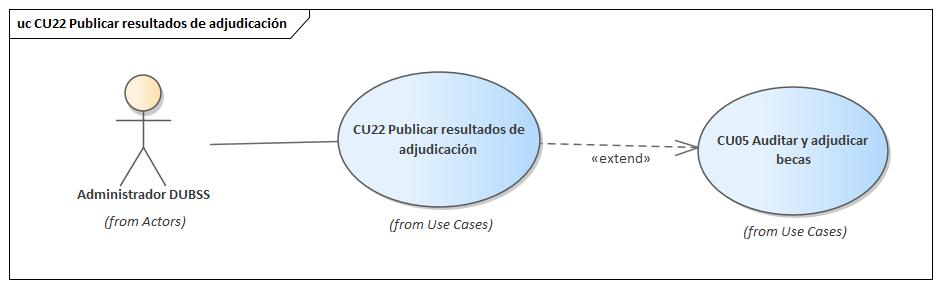
\includegraphics[width=0.8\textwidth,height=0.4\textheight,keepaspectratio]{images/074_CU22_Publicar_Resultados_Adjudicacion.jpg}

\smallskip
\noindent\raggedright\textit{Nota.} Elaboración propia.
\end{figure}

\refstepcounter{table}\label{tab:detalle_cu22}
\addcontentsline{lot}{table}{\protect\numberline{\thetable}Detalle del CU-22: Publicar resultados de adjudicación}
\noindent\textbf{Tabla~\thetable}\par\nopagebreak
\noindent\textit{Detalle del CU-22: Publicar resultados de adjudicación}\par\nopagebreak
\begingroup\small\linespread{1}\selectfont
\begin{longtable}{>{\raggedright\arraybackslash}p{2.9cm} >{\raggedright\arraybackslash}p{12.6cm}}
\toprule
\textbf{Caso de Uso} & \textbf{CU-22. Publicar resultados de adjudicación} \\
\midrule
\endfirsthead
\toprule
\textbf{Caso de Uso} & \textbf{CU-22. Publicar resultados de adjudicación} \\
\midrule
\endhead
\endfoot
\bottomrule
\multicolumn{2}{l}{\textit{Nota.} Elaboración propia.} \\
\endlastfoot
\textbf{Propósito} & Dar a conocer de forma oficial y transparente los resultados de la adjudicación de la Beca Comedor de una convocatoria y poner fin al proceso de selección. \\
\midrule
\textbf{Descripción} & Este caso de uso describe cómo el Administrador DUBSS, una vez decididas todas las adjudicaciones, publica los resultados de la convocatoria. Al publicar, el sistema registra la publicación, pasa la convocatoria a «publicada», la anota en la bitácora y avisa a cada finalista con decisión su resultado por bandeja, notificación push y correo (CU-EXTRA-01). La publicación no se puede deshacer, no exige el acta (que se genera después, CU-08) y desde ese momento no se registran ni modifican decisiones. Los postulantes consultan la lista de adjudicados y su propio resultado. Extiende el CU-05. Respalda el RF-17. \\
\midrule
\textbf{Actores} & Administrador DUBSS. \\
\midrule
\textbf{Actor Iniciador} & Administrador DUBSS. \\
\midrule
\textbf{Precondición} & \vspace{-\baselineskip}\begin{cuvin}
    \item El Administrador DUBSS está autenticado en el sistema (CU-01) con el rol Administrador DUBSS.
    \item La convocatoria está cerrada y ningún finalista queda en estado «calificada»: cada uno está adjudicado, no adjudicado, archivado o devuelto (CU-05).
    \item Los resultados de la convocatoria no han sido publicados previamente.
\end{cuvin} \\
\midrule
\textbf{Proceso} & \textbf{Flujo principal.}
\begin{cupasos}
    \item El Administrador DUBSS selecciona la opción «Publicar resultados» y elige la convocatoria.
    \item El sistema muestra el resumen: adjudicados y no adjudicados con el puntaje final de cada finalista.
    \item El Administrador DUBSS revisa los resultados, pulsa «Publicar» y confirma en una ventana que avisa que la publicación no se puede deshacer.
    \item El sistema verifica que la convocatoria exista y esté cerrada, que no esté publicada y que no queden finalistas en estado «calificada».
    \item El sistema registra la publicación con el usuario que la realiza y la fecha, la anota en la bitácora y pasa la convocatoria a «publicada», en una misma operación.
    \item El sistema crea un aviso para cada finalista con decisión y se lo envía por bandeja, notificación push y correo.
    \item El sistema confirma la publicación; la lista de adjudicados queda consultable por los postulantes (CU-04).
\end{cupasos} \\
 & \textbf{Flujos alternativos.}
\begin{cuvin}
    \item A1 (paso 4): si quedan finalistas en estado «calificada», el sistema no permite publicar e indica cuántos faltan (409, ERR\_PUB\_01).
    \item A2 (pasos 1 y 4): si los resultados ya fueron publicados, el sistema no registra otra publicación y muestra la existente (409, ERR\_PUB\_02); un doble clic recibe el mismo 409.
    \item A3 (paso 4): si la convocatoria no existe (404, ERR\_PRI\_01) o no está cerrada (409, ERR\_PUB\_03), el sistema vuelve a la lista de convocatorias.
    \item A4 (paso 6): si falla el envío de un aviso, la publicación queda registrada, el aviso queda en la bandeja y se reintenta el push y el correo; un fallo de envío nunca deshace la publicación.
    \item A5 (paso 3): si el Administrador DUBSS cancela la operación, no se publica ningún resultado.
\end{cuvin} \\
\midrule
\textbf{Postcondición} & \vspace{-\baselineskip}\begin{cuvin}
    \item Los resultados de la convocatoria quedan publicados y registrados con su responsable y fecha.
    \item Cada finalista con decisión recibe un aviso con su resultado; los adjudicados son el punto de partida del padrón de becados (CU-23).
    \item No se registran ni modifican decisiones de la convocatoria, y la publicación queda anotada en la bitácora (CU-25).
\end{cuvin} \\
\midrule
\textbf{Excepciones} & \vspace{-\baselineskip}\begin{cuvin}
    \item Autenticación inválida o sesión expirada.
    \item Falta de permisos suficientes (el usuario no tiene el rol Administrador DUBSS).
    \item Finalistas pendientes de decisión.
    \item Error al enviar el push o el correo (no deshace la publicación).
    \item Error de conexión con el servidor o la base de datos.
\end{cuvin} \\
\end{longtable}
\endgroup
\addtocounter{table}{-1}

\subsubsection{5.4.23. CU-23 Gestionar padrón de becados (baja, suspensión, reemplazo)}\label{sec:cap5_cu23}

\begin{figure}[H]
\caption{Diagrama de contexto del CU-23}
\label{fig:ctx_cu23}
\centering
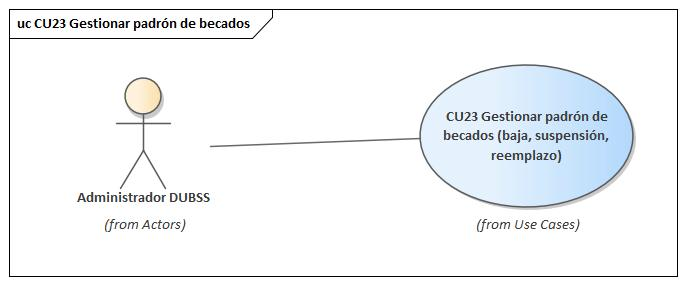
\includegraphics[width=0.8\textwidth,height=0.4\textheight,keepaspectratio]{images/075_CU23_Gestionar_Padron_Becados.jpg}

\smallskip
\noindent\raggedright\textit{Nota.} Elaboración propia.
\end{figure}

\refstepcounter{table}\label{tab:detalle_cu23}
\addcontentsline{lot}{table}{\protect\numberline{\thetable}Detalle del CU-23: Gestionar padrón de becados (baja, suspensión, reemplazo)}
\noindent\textbf{Tabla~\thetable}\par\nopagebreak
\noindent\textit{Detalle del CU-23: Gestionar padrón de becados (baja, suspensión, reemplazo)}\par\nopagebreak
\begingroup\small\linespread{1}\selectfont
\begin{longtable}{>{\raggedright\arraybackslash}p{2.9cm} >{\raggedright\arraybackslash}p{12.6cm}}
\toprule
\textbf{Caso de Uso} & \textbf{CU-23. Gestionar padrón de becados (baja, suspensión, reemplazo)} \\
\midrule
\endfirsthead
\toprule
\textbf{Caso de Uso} & \textbf{CU-23. Gestionar padrón de becados (baja, suspensión, reemplazo)} \\
\midrule
\endhead
\endfoot
\bottomrule
\multicolumn{2}{l}{\textit{Nota.} Elaboración propia.} \\
\endlastfoot
\textbf{Propósito} & Mantener actualizado el padrón de becados vigentes de la gestión, registrando bajas, suspensiones y reemplazos, del cual dependen las planillas de asistencia. \\
\midrule
\textbf{Descripción} & Este caso de uso describe cómo el Administrador DUBSS consulta el padrón de becados de una convocatoria y registra sobre él las bajas, suspensiones y reemplazos que ocurren durante la gestión. Cada cambio actualiza el estado de la beca y queda registrado como un movimiento con su motivo, responsable y fecha. En un reemplazo, el cupo liberado se asigna al siguiente postulante priorizado. Los cambios se reflejan en las planillas de asistencia generadas posteriormente (CU-09). Respalda el RF-18. \\
\midrule
\textbf{Actores} & Administrador DUBSS. \\
\midrule
\textbf{Actor Iniciador} & Administrador DUBSS. \\
\midrule
\textbf{Precondición} & \vspace{-\baselineskip}\begin{cuvin}
    \item El Administrador DUBSS está autenticado en el sistema (CU-01) con el rol Administrador DUBSS.
    \item Los resultados de adjudicación de la convocatoria fueron publicados (CU-22) y existen becas registradas.
\end{cuvin} \\
\midrule
\textbf{Proceso} & \textbf{Flujo principal A: consultar el padrón.}
\begin{cupasos}
    \item El Administrador DUBSS selecciona la opción «Padrón de becados» y la convocatoria.
    \item El sistema muestra las becas de la convocatoria con el nombre, CI y carrera del becado y el estado de la beca (vigente, suspendida o baja).
\end{cupasos} \\
 & \textbf{Flujo principal B: dar de baja o suspender una beca.}
\begin{cupasos}
    \item El Administrador DUBSS selecciona una beca vigente y la opción «Dar de baja» o «Suspender».
    \item El sistema solicita el motivo.
    \item El Administrador DUBSS registra el motivo y confirma.
    \item El sistema actualiza el estado de la beca a «baja» o «suspendida», según corresponda.
    \item El sistema registra el movimiento (tipo, motivo, usuario y fecha) y deja constancia en la bitácora.
\end{cupasos} \\
 & \textbf{Flujo principal C: reemplazar un cupo liberado.}
\begin{cupasos}
    \item El Administrador DUBSS selecciona una beca dada de baja y la opción «Reemplazar».
    \item El sistema muestra al siguiente postulante de la lista priorizada disponible para ocupar el cupo.
    \item El Administrador DUBSS confirma el reemplazo.
    \item El sistema crea una nueva beca vigente para el postulante reemplazante.
    \item El sistema registra el movimiento de reemplazo, vinculando la beca liberada con la beca reemplazante, y deja constancia en la bitácora.
\end{cupasos} \\
 & \textbf{Flujos alternativos.}
\begin{cuvin}
    \item A1 (flujo B, paso 3): si no se registra el motivo, el sistema no permite completar la operación.
    \item A2 (flujo B, paso 1): si la beca no está vigente, el sistema no permite darla de baja ni suspenderla.
    \item A3 (flujo C, paso 1): si la beca seleccionada no ha sido dada de baja, el sistema no permite el reemplazo.
    \item A4 (flujo C, paso 2): si no existe un postulante disponible para ocupar el cupo, el sistema lo informa y no realiza el reemplazo.
    \item A5 (flujos B y C): si el Administrador DUBSS cancela la operación, el padrón no se modifica.
\end{cuvin} \\
\midrule
\textbf{Postcondición} & \vspace{-\baselineskip}\begin{cuvin}
    \item El padrón refleja el estado actualizado de cada beca y cada cambio queda registrado como movimiento y en la bitácora.
    \item Las planillas de asistencia que se generen posteriormente (CU-09) consideran solo las becas vigentes.
\end{cuvin} \\
\midrule
\textbf{Excepciones} & \vspace{-\baselineskip}\begin{cuvin}
    \item Autenticación inválida o sesión expirada.
    \item Falta de permisos suficientes (el usuario no tiene el rol Administrador DUBSS).
    \item Operación no permitida para el estado actual de la beca.
    \item Error de conexión con el servidor o la base de datos.
\end{cuvin} \\
\end{longtable}
\endgroup
\addtocounter{table}{-1}

\subsubsection{5.4.24. CU-24 Consultar historial de asistencia y estado de beca}\label{sec:cap5_cu24}

\begin{figure}[H]
\caption{Diagrama de contexto del CU-24}
\label{fig:ctx_cu24}
\centering
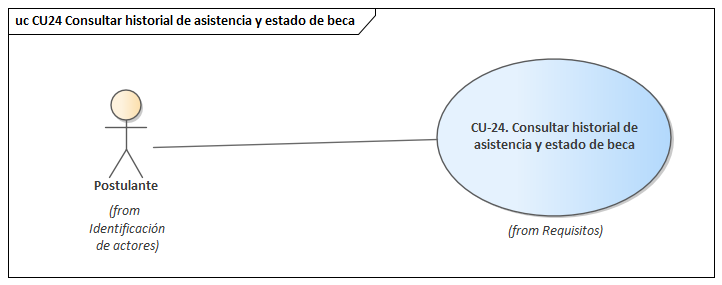
\includegraphics[width=0.8\textwidth,height=0.4\textheight,keepaspectratio]{images/049_CU24_Consultar_Historial_Asistencia_Beca.png}

\smallskip
\noindent\raggedright\textit{Nota.} Elaboración propia.
\end{figure}

\refstepcounter{table}\label{tab:detalle_cu24}
\addcontentsline{lot}{table}{\protect\numberline{\thetable}Detalle del CU-24: Consultar historial de asistencia y estado de beca}
\noindent\textbf{Tabla~\thetable}\par\nopagebreak
\noindent\textit{Detalle del CU-24: Consultar historial de asistencia y estado de beca}\par\nopagebreak
\begingroup\small\linespread{1}\selectfont
\begin{longtable}{>{\raggedright\arraybackslash}p{2.9cm} >{\raggedright\arraybackslash}p{12.6cm}}
\toprule
\textbf{Caso de Uso} & \textbf{CU-24. Consultar historial de asistencia y estado de beca} \\
\midrule
\endfirsthead
\toprule
\textbf{Caso de Uso} & \textbf{CU-24. Consultar historial de asistencia y estado de beca} \\
\midrule
\endhead
\endfoot
\bottomrule
\multicolumn{2}{l}{\textit{Nota.} Elaboración propia.} \\
\endlastfoot
\textbf{Propósito} & Permitir al Postulante adjudicado (becado) consultar su historial de asistencia al comedor y el estado vigente de su beca. \\
\midrule
\textbf{Descripción} & Este caso de uso describe cómo el becado consulta, desde el portal web o la aplicación móvil, las fechas de asistencia registradas en la gestión vigente y el estado de su beca (vigente, suspendida o dada de baja) con su motivo, de modo que pueda verificar el cumplimiento de los requisitos de asistencia y conservar su beneficio. Es una consulta de solo lectura que utiliza los datos registrados en el CU-10 y en el padrón de becados (CU-23). Respalda el RF-19. \\
\midrule
\textbf{Actores} & Postulante (becado, es decir, Postulante adjudicado). \\
\midrule
\textbf{Actor Iniciador} & Postulante (becado). \\
\midrule
\textbf{Precondición} & \vspace{-\baselineskip}\begin{cuvin}
    \item El Postulante está autenticado en el sistema (CU-01).
    \item La postulación del Postulante fue adjudicada y figura en el padrón de becados.
\end{cuvin} \\
\midrule
\textbf{Proceso} & \textbf{Flujo principal.}
\begin{cupasos}
    \item El becado accede a la opción «Mi beca».
    \item El sistema verifica que el usuario figure en el padrón de becados de la gestión.
    \item El sistema muestra el estado de la beca (vigente, suspendida o dada de baja), la gestión académica y la fecha de adjudicación.
    \item El sistema muestra el historial de asistencia de la gestión vigente: las fechas de asistencia registradas en el comedor y el total acumulado.
    \item El becado revisa la información y, opcionalmente, filtra el historial por rango de fechas.
\end{cupasos} \\
 & \textbf{Flujos alternativos.}
\begin{cuvin}
    \item A1 (paso 2): si el usuario no figura como becado, el sistema informa que no cuenta con una beca vigente y lo redirige a la consulta del estado de su postulación (CU-04).
    \item A2 (paso 4): si aún no existen asistencias registradas, el sistema muestra un mensaje informativo.
    \item A3 (paso 3): si la beca está suspendida o dada de baja, el sistema muestra el estado y el motivo registrado por el Administrador (CU-23); el historial de asistencia se conserva y sigue siendo consultable.
    \item A4 (paso 1): si el usuario intenta acceder a la información de otro becado, el sistema deniega el acceso.
\end{cuvin} \\
\midrule
\textbf{Postcondición} & \vspace{-\baselineskip}\begin{cuvin}
    \item El becado visualiza su historial de asistencia y el estado de su beca; la consulta no modifica ningún dato del sistema.
\end{cuvin} \\
\midrule
\textbf{Excepciones} & \vspace{-\baselineskip}\begin{cuvin}
    \item Autenticación inválida o sesión expirada.
    \item Falta de permisos suficientes (el usuario solo puede acceder a su propia información).
    \item Usuario sin beca adjudicada.
    \item Error de conexión con el servidor o la base de datos.
\end{cuvin} \\
\end{longtable}
\endgroup
\addtocounter{table}{-1}

\subsubsection{5.4.25. CU-25 Consultar bitácora de acciones}\label{sec:cap5_cu25}

\begin{figure}[H]
\caption{Diagrama de contexto del CU-25}
\label{fig:ctx_cu25}
\centering
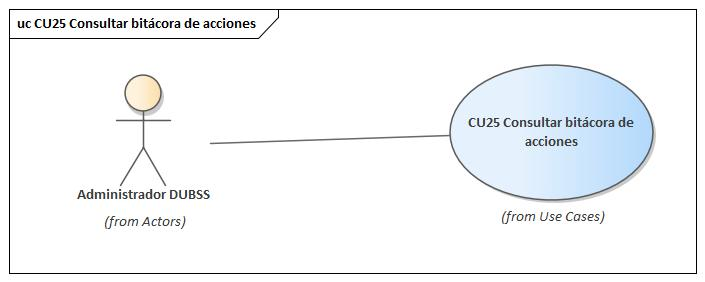
\includegraphics[width=0.8\textwidth,height=0.4\textheight,keepaspectratio]{images/076_CU25_Consultar_Bitacora_Acciones.jpg}

\smallskip
\noindent\raggedright\textit{Nota.} Elaboración propia.
\end{figure}

\refstepcounter{table}\label{tab:detalle_cu25}
\addcontentsline{lot}{table}{\protect\numberline{\thetable}Detalle del CU-25: Consultar bitácora de acciones}
\noindent\textbf{Tabla~\thetable}\par\nopagebreak
\noindent\textit{Detalle del CU-25: Consultar bitácora de acciones}\par\nopagebreak
\begingroup\small\linespread{1}\selectfont
\begin{longtable}{>{\raggedright\arraybackslash}p{2.9cm} >{\raggedright\arraybackslash}p{12.6cm}}
\toprule
\textbf{Caso de Uso} & \textbf{CU-25. Consultar bitácora de acciones} \\
\midrule
\endfirsthead
\toprule
\textbf{Caso de Uso} & \textbf{CU-25. Consultar bitácora de acciones} \\
\midrule
\endhead
\endfoot
\bottomrule
\multicolumn{2}{l}{\textit{Nota.} Elaboración propia.} \\
\endlastfoot
\textbf{Propósito} & Permitir al Administrador DUBSS consultar el registro de las acciones relevantes realizadas en el sistema, para garantizar la trazabilidad de las decisiones y facilitar las auditorías. \\
\midrule
\textbf{Descripción} & Este caso de uso describe cómo el Administrador DUBSS consulta la bitácora del sistema, en la que se registran automáticamente las acciones relevantes (auditoría, devolución, adjudicación, publicación, cambios en el padrón y cambios de roles) con el usuario, la acción, la entidad o expediente afectado, la fecha y la hora. La bitácora puede filtrarse por usuario, tipo de acción y rango de fechas. Es una consulta de solo lectura: los registros no pueden editarse ni eliminarse. Respalda el RF-20. \\
\midrule
\textbf{Actores} & Administrador DUBSS. \\
\midrule
\textbf{Actor Iniciador} & Administrador DUBSS. \\
\midrule
\textbf{Precondición} & \vspace{-\baselineskip}\begin{cuvin}
    \item El Administrador DUBSS está autenticado en el sistema (CU-01) con el rol Administrador DUBSS.
\end{cuvin} \\
\midrule
\textbf{Proceso} & \textbf{Flujo principal.}
\begin{cupasos}
    \item El Administrador DUBSS selecciona la opción «Bitácora de acciones».
    \item El sistema muestra los registros de la bitácora ordenados del más reciente al más antiguo y paginados, con la fecha y hora, el usuario, la acción, la entidad o expediente afectado y el detalle de cada registro.
    \item El Administrador DUBSS ingresa los filtros de búsqueda: usuario, tipo de acción y rango de fechas.
    \item El sistema muestra los registros que cumplen los filtros.
\end{cupasos} \\
 & \textbf{Flujos alternativos.}
\begin{cuvin}
    \item A1 (paso 4): si ningún registro cumple los filtros, el sistema muestra un mensaje informativo.
    \item A2 (paso 3): si la fecha final del rango es anterior a la inicial, el sistema lo indica y permite corregirla.
    \item A3 (paso 2): las acciones ejecutadas por el sistema o por el módulo de IA se muestran sin usuario asociado.
\end{cuvin} \\
\midrule
\textbf{Postcondición} & \vspace{-\baselineskip}\begin{cuvin}
    \item El Administrador DUBSS visualiza los registros de la bitácora; la consulta no modifica ningún dato del sistema.
\end{cuvin} \\
\midrule
\textbf{Excepciones} & \vspace{-\baselineskip}\begin{cuvin}
    \item Autenticación inválida o sesión expirada.
    \item Falta de permisos suficientes (el usuario no tiene el rol Administrador DUBSS).
    \item Error de conexión con el servidor o la base de datos.
\end{cuvin} \\
\end{longtable}
\endgroup
\addtocounter{table}{-1}

\subsubsection{5.4.26. CU-26 Parametrizar modelo de preselección y reprocesar puntajes}\label{sec:cap5_cu26}

\begin{figure}[H]
\caption{Diagrama de contexto del CU-26}
\label{fig:ctx_cu26}
\centering
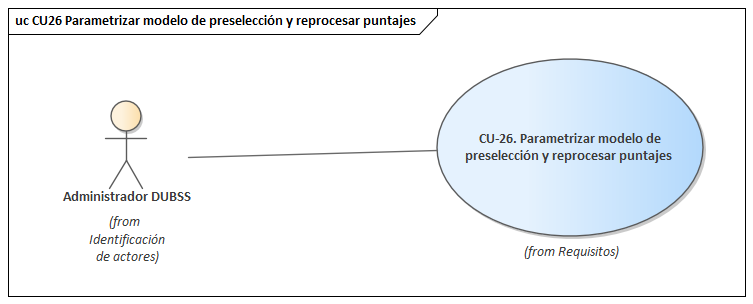
\includegraphics[width=0.8\textwidth,height=0.4\textheight,keepaspectratio]{images/050_CU26_Parametrizar_Modelo_Preseleccion.png}

\smallskip
\noindent\raggedright\textit{Nota.} Elaboración propia.
\end{figure}

\refstepcounter{table}\label{tab:detalle_cu26}
\addcontentsline{lot}{table}{\protect\numberline{\thetable}Detalle del CU-26: Parametrizar modelo de preselección y reprocesar puntajes}
\noindent\textbf{Tabla~\thetable}\par\nopagebreak
\noindent\textit{Detalle del CU-26: Parametrizar modelo de preselección y reprocesar puntajes}\par\nopagebreak
\begingroup\small\linespread{1}\selectfont
\begin{longtable}{>{\raggedright\arraybackslash}p{2.9cm} >{\raggedright\arraybackslash}p{12.6cm}}
\toprule
\textbf{Caso de Uso} & \textbf{CU-26. Parametrizar modelo de preselección y reprocesar puntajes} \\
\midrule
\endfirsthead
\toprule
\textbf{Caso de Uso} & \textbf{CU-26. Parametrizar modelo de preselección y reprocesar puntajes} \\
\midrule
\endhead
\endfoot
\bottomrule
\multicolumn{2}{l}{\textit{Nota.} Elaboración propia.} \\
\endlastfoot
\textbf{Propósito} & Permitir al Administrador DUBSS ajustar los criterios y ponderaciones del modelo de preselección y reprocesar los puntajes de las postulaciones de una convocatoria. \\
\midrule
\textbf{Descripción} & Este caso de uso describe cómo el Administrador DUBSS consulta y modifica los parámetros del modelo de IA (criterios y ponderaciones de las variables socioeconómicas y académicas), los guarda como una nueva versión y, si lo decide, reprocesa los puntajes de una convocatoria. Cada recálculo conserva el puntaje anterior para fines de trazabilidad. Extiende al CU-03. Respalda el RF-21. \\
\midrule
\textbf{Actores} & Administrador DUBSS. \\
\midrule
\textbf{Actor Iniciador} & Administrador DUBSS. \\
\midrule
\textbf{Precondición} & \vspace{-\baselineskip}\begin{cuvin}
    \item El Administrador DUBSS está autenticado en el sistema (CU-01) y cuenta con privilegios de administración.
    \item El módulo de IA está disponible.
    \item Para reprocesar: la convocatoria seleccionada tiene postulaciones precalificadas (CU-03).
\end{cuvin} \\
\midrule
\textbf{Proceso} & \textbf{Flujo principal.}
\begin{cupasos}
    \item El Administrador accede a la opción «Parámetros del modelo».
    \item El sistema muestra los criterios y ponderaciones vigentes (variables: ingresos familiares, dependientes, procedencia, carrera, patrimonio, estado de vulnerabilidad y promedio académico), con su versión y fecha de vigencia.
    \item El Administrador modifica los criterios o ponderaciones necesarios (valores y rangos por definir con la DUBSS).
    \item El sistema valida los valores ingresados (rangos permitidos y consistencia entre ponderaciones).
    \item El Administrador guarda los cambios y el sistema crea una nueva versión de los parámetros, conservando las versiones anteriores.
    \item El Administrador selecciona la convocatoria y solicita «Reprocesar puntajes».
    \item El sistema muestra el resumen del reprocesamiento (convocatoria y cantidad de postulaciones afectadas) y solicita confirmación.
    \item El Administrador confirma.
    \item El sistema ejecuta el reprocesamiento en lote, invocando el cálculo del CU-03 para cada postulación, y muestra el avance.
    \item El sistema registra la fecha de cada recálculo y conserva el puntaje anterior de cada postulación.
    \item El sistema muestra la lista priorizada actualizada (CU-06) y registra la acción en la bitácora (CU-25).
\end{cupasos} \\
 & \textbf{Flujos alternativos.}
\begin{cuvin}
    \item A1 (paso 4): si los valores están fuera de rango o son inconsistentes, el sistema indica los errores y no guarda los parámetros.
    \item A2 (paso 5): si el Administrador guarda los parámetros sin reprocesar, la nueva versión se aplica únicamente a las postulaciones que se precalifiquen a partir de ese momento.
    \item A3 (paso 6): si ya se publicaron resultados de adjudicación en la convocatoria (CU-22), el sistema advierte o bloquea el reprocesamiento (regla por definir con la DUBSS).
    \item A4 (paso 6): si hay un reprocesamiento en curso para la misma convocatoria, el sistema impide lanzar otro de forma simultánea.
    \item A5 (paso 9): si el cálculo falla para algunas postulaciones, el sistema continúa con las demás, lista las fallidas y permite reintentarlas.
    \item A6 (paso 7): el Administrador puede cancelar el reprocesamiento antes de confirmarlo, sin que se modifique ningún puntaje.
\end{cuvin} \\
\midrule
\textbf{Postcondición} & \vspace{-\baselineskip}\begin{cuvin}
    \item Los nuevos parámetros quedan guardados como una versión vigente, y las versiones anteriores se conservan.
    \item Los puntajes reprocesados quedan registrados con su fecha de recálculo y el puntaje anterior se conserva; la lista priorizada refleja el nuevo orden.
    \item La acción queda registrada en la bitácora.
\end{cuvin} \\
\midrule
\textbf{Excepciones} & \vspace{-\baselineskip}\begin{cuvin}
    \item Autenticación inválida o sesión expirada.
    \item Falta de permisos suficientes (el usuario no tiene el rol Administrador DUBSS).
    \item Parámetros ingresados no válidos.
    \item Módulo de IA no disponible durante el reprocesamiento.
    \item Error de conexión con el servidor o la base de datos.
\end{cuvin} \\
\end{longtable}
\endgroup
\addtocounter{table}{-1}

% ------------------------------------------------------------------------------
% 5.5. DIAGRAMA GENERAL DE CASOS DE USO
% ------------------------------------------------------------------------------
\wfa{\wn{5.5}. Diagrama General de Casos de Uso}\label{sec:cap5_diagrama_general}

La Figura~\ref{fig:diagrama_general_cu} presenta el diagrama general de casos de uso del sistema, que integra los actores identificados y los casos de uso priorizados y detallados en las secciones anteriores.

\begin{figure}[H]
\caption{Diagrama general de casos de uso del Sistema Web y Móvil de Postulación y Preselección de la Beca Comedor}
\label{fig:diagrama_general_cu}
\centering
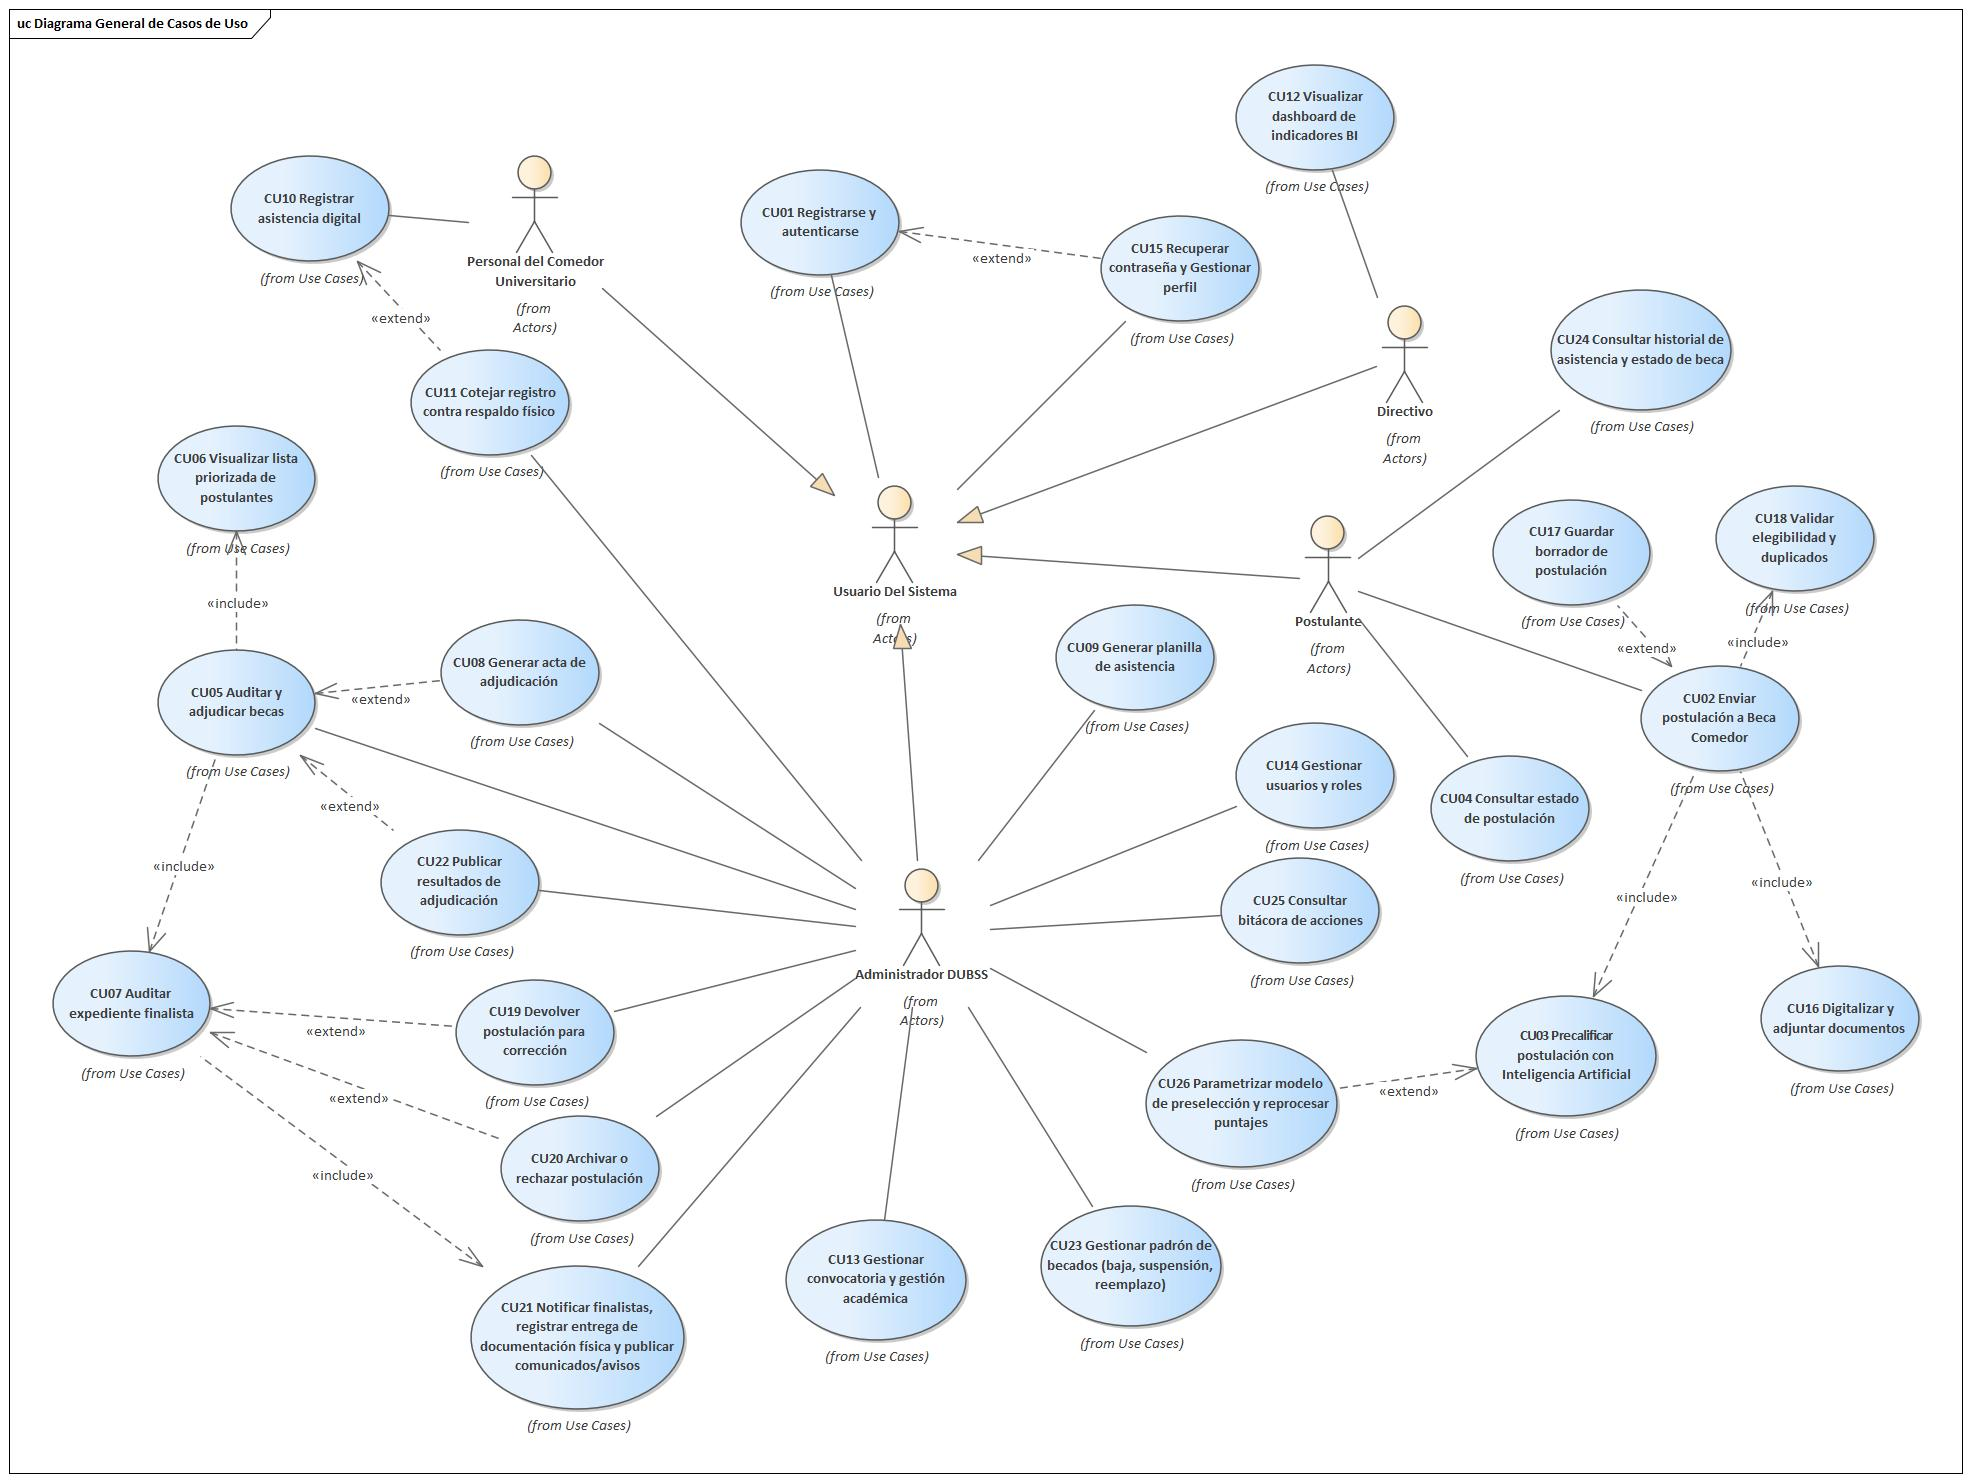
\includegraphics[width=\textwidth,height=0.85\textheight,keepaspectratio]{images/019_Diagrama_General_CU.jpg}

\smallskip
\noindent\raggedright\textit{Nota.} Elaboración propia.
\end{figure}



% ==============================================================================
% 3.3 ANÁLISIS (flujo de trabajo PUDS)
% Reutiliza el cap. 6 de main.tex.
% ==============================================================================
\subsection{3.3. Análisis}\label{sec:v2_analisis}

Este flujo de trabajo del PUDS define la arquitectura de análisis en paquetes, analiza cada caso de uso y analiza cada paquete.

% ------------------------------------------------------------------------------
% 6.1. ANÁLISIS DE LA ARQUITECTURA
% ------------------------------------------------------------------------------
\wfa{\wn{6}.1. Análisis de la Arquitectura}\label{sec:cap6_arquitectura}

% [PENDIENTE]: Redactar el análisis de la arquitectura.

\wfb{\wn{6}.1.1. Identificación de Paquetes}\label{sec:cap6_identificacion_paquetes}

Con el fin de organizar los veintiséis casos de uso del sistema, se agruparon por afinidad funcional en seis paquetes de análisis, de modo que cada uno concentre las responsabilidades de un área del proceso de la Beca Comedor. La Figura~\ref{fig:identificacion_paquetes} presenta los paquetes identificados.

\begin{figure}[H]
\caption{Identificación de paquetes}
\label{fig:identificacion_paquetes}
\centering
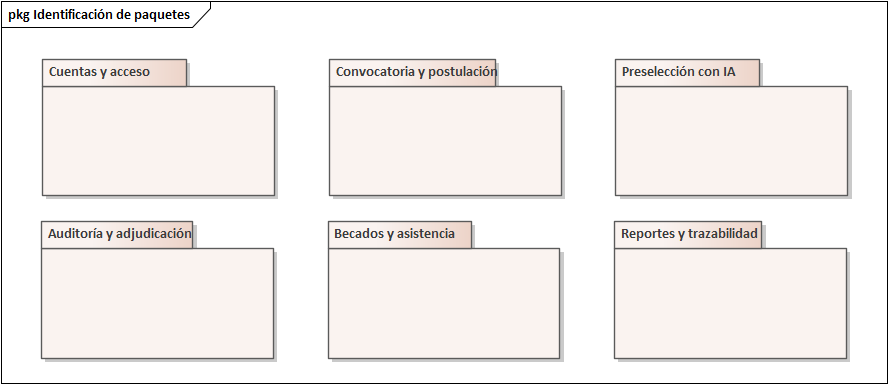
\includegraphics[width=\textwidth,height=0.85\textheight,keepaspectratio]{images/031_Identificacion_de_Paquetes.png}

\smallskip
\noindent\raggedright\textit{Nota.} Elaboración propia.
\end{figure}

Los paquetes identificados se describen a continuación:

\begin{itemize}
    \item \textbf{Cuentas y acceso:} reúne el registro, la autenticación, la recuperación de contraseña, la gestión de perfil y la administración de usuarios y roles.
    \item \textbf{Convocatoria y postulación:} comprende la gestión de convocatorias y el proceso que realiza el postulante: envío de la postulación, digitalización de documentos, validación de elegibilidad, guardado de borradores y consulta del estado.
    \item \textbf{Preselección con IA:} contiene la precalificación automática de las postulaciones mediante Inteligencia Artificial y la parametrización del modelo.
    \item \textbf{Auditoría y adjudicación:} agrupa la lista priorizada de postulantes, la auditoría de expedientes finalistas, la devolución o archivo de postulaciones, la notificación a finalistas y la adjudicación con publicación de resultados.
    \item \textbf{Becados y asistencia:} abarca la gestión del padrón de becados, la generación de planillas, el registro y cotejo de la asistencia y la consulta del historial por el becado.
    \item \textbf{Reportes y trazabilidad:} incluye el dashboard de indicadores de Business Intelligence y la consulta de la bitácora de acciones.
\end{itemize}

\wfb{\wn{6}.1.2. Relación de Paquetes}\label{sec:cap6_relacion_paquetes}

Una vez identificados los paquetes, se establece la relación de cada uno con los casos de uso que contiene. Las Figuras~\ref{fig:rel_cuentas}, \ref{fig:rel_convocatoria}, \ref{fig:rel_preseleccion}, \ref{fig:rel_auditoria}, \ref{fig:rel_becados} y~\ref{fig:rel_reportes} muestran, para cada paquete, sus casos de uso asociados mediante dependencias de trazabilidad («trace») y las relaciones de inclusión («include») y extensión («extend») entre ellos.

El paquete Cuentas y Acceso se relaciona, mediante dependencias de trazabilidad, con los casos de uso CU-01, CU-14 y CU-15; además, CU-15 extiende a CU-01, como se muestra en la Figura~\ref{fig:rel_cuentas}.

\begin{figure}[H]
\caption{Relación del paquete Cuentas y Acceso}
\label{fig:rel_cuentas}
\centering
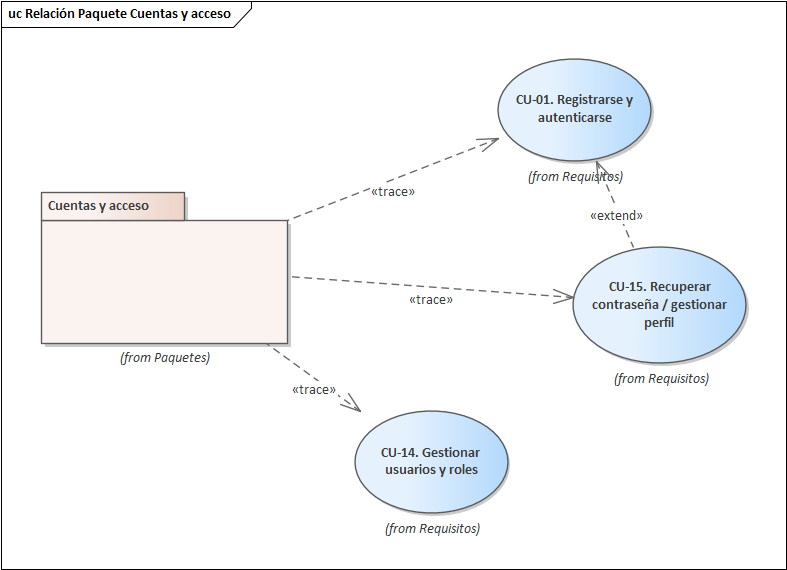
\includegraphics[width=\textwidth,height=0.85\textheight,keepaspectratio]{images/032_Relacion_Cuentas_Acceso.png}

\smallskip
\noindent\raggedright\textit{Nota.} Elaboración propia.
\end{figure}

El paquete Convocatoria y Postulación se relaciona con los casos de uso CU-02, CU-04, CU-13, CU-16, CU-17 y CU-18. En este paquete, CU-02 incluye a CU-16, CU-18 y CU-03 (este último perteneciente al paquete Preselección con IA), y CU-17 extiende a CU-02, como se muestra en la Figura~\ref{fig:rel_convocatoria}.

\begin{figure}[H]
\caption{Relación del paquete Convocatoria y Postulación}
\label{fig:rel_convocatoria}
\centering
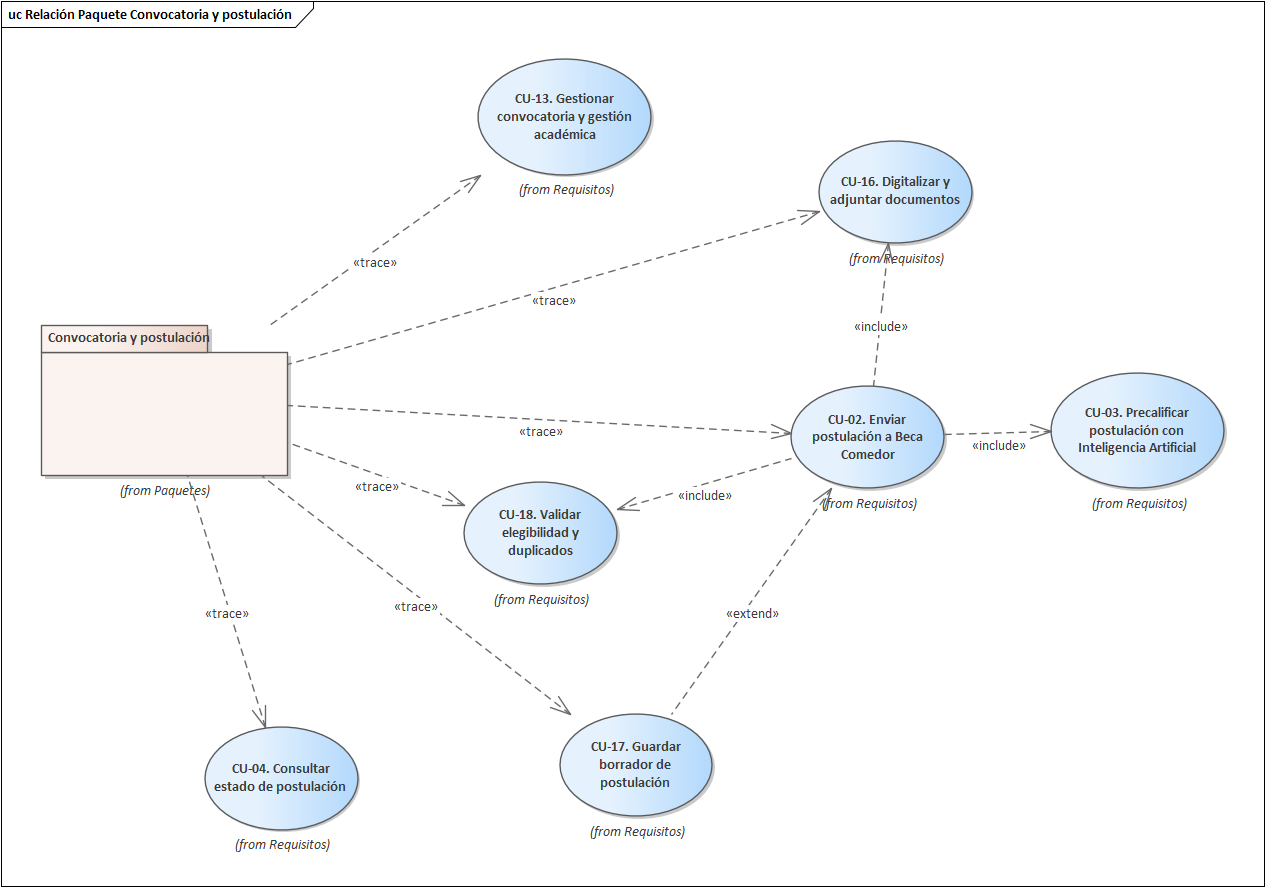
\includegraphics[width=\textwidth,height=0.85\textheight,keepaspectratio]{images/033_Relacion_Convocatoria_Postulacion.png}

\smallskip
\noindent\raggedright\textit{Nota.} Elaboración propia.
\end{figure}

El paquete Preselección con IA se relaciona con los casos de uso CU-03 y CU-26, donde CU-26 extiende a CU-03, como se muestra en la Figura~\ref{fig:rel_preseleccion}.

\begin{figure}[H]
\caption{Relación del paquete Preselección con IA}
\label{fig:rel_preseleccion}
\centering
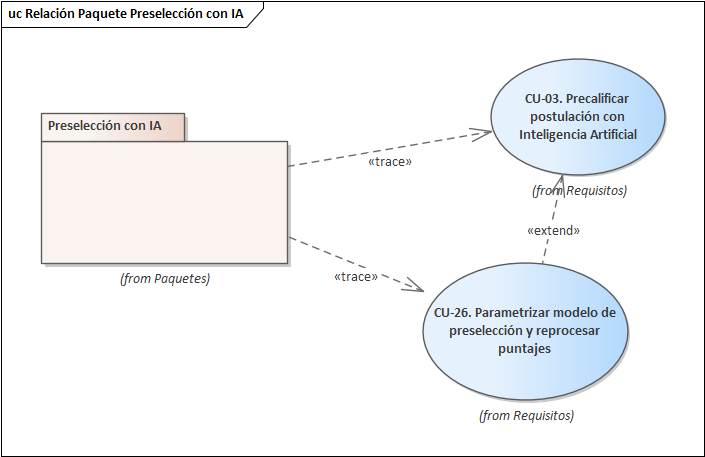
\includegraphics[width=\textwidth,height=0.85\textheight,keepaspectratio]{images/034_Relacion_Preseleccion_IA.png}

\smallskip
\noindent\raggedright\textit{Nota.} Elaboración propia.
\end{figure}

El paquete Auditoría y Adjudicación se relaciona con los casos de uso CU-05, CU-06, CU-07, CU-08, CU-19, CU-20, CU-21 y CU-22. CU-05 incluye a CU-06 y CU-07; CU-07 incluye a CU-21; CU-19 y CU-20 extienden a CU-07; y CU-08 y CU-22 extienden a CU-05, como se muestra en la Figura~\ref{fig:rel_auditoria}.

\begin{figure}[H]
\caption{Relación del paquete Auditoría y Adjudicación}
\label{fig:rel_auditoria}
\centering
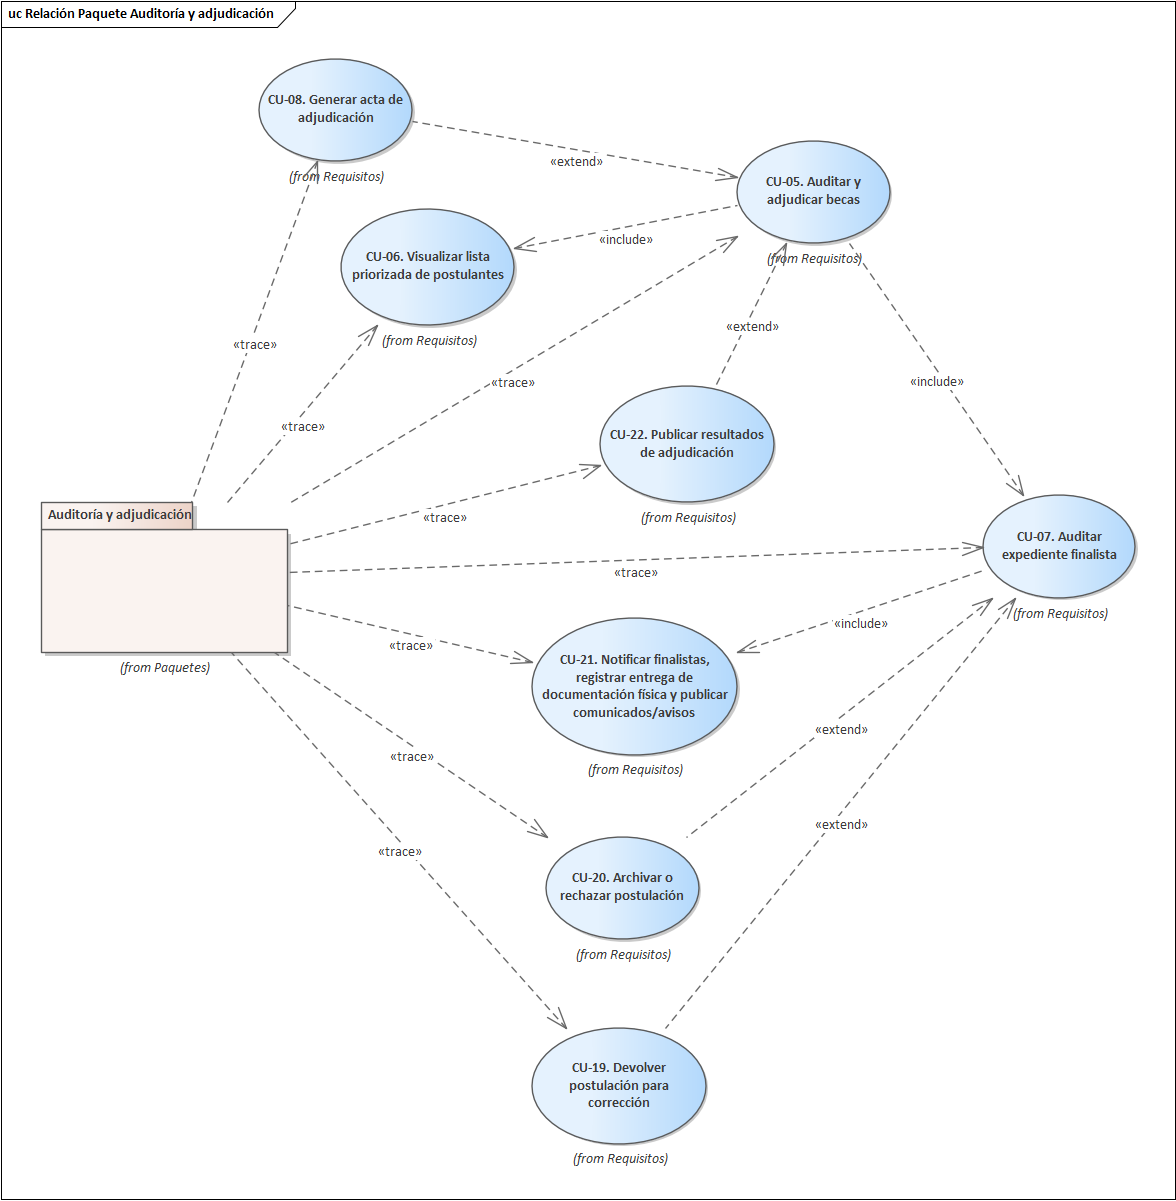
\includegraphics[width=\textwidth,height=0.85\textheight,keepaspectratio]{images/035_Relacion_Auditoria_Adjudicacion.png}

\smallskip
\noindent\raggedright\textit{Nota.} Elaboración propia.
\end{figure}

El paquete Becados y Asistencia se relaciona con los casos de uso CU-09, CU-10, CU-11, CU-23 y CU-24, donde CU-11 extiende a CU-10, como se muestra en la Figura~\ref{fig:rel_becados}.

\begin{figure}[H]
\caption{Relación del paquete Becados y Asistencia}
\label{fig:rel_becados}
\centering
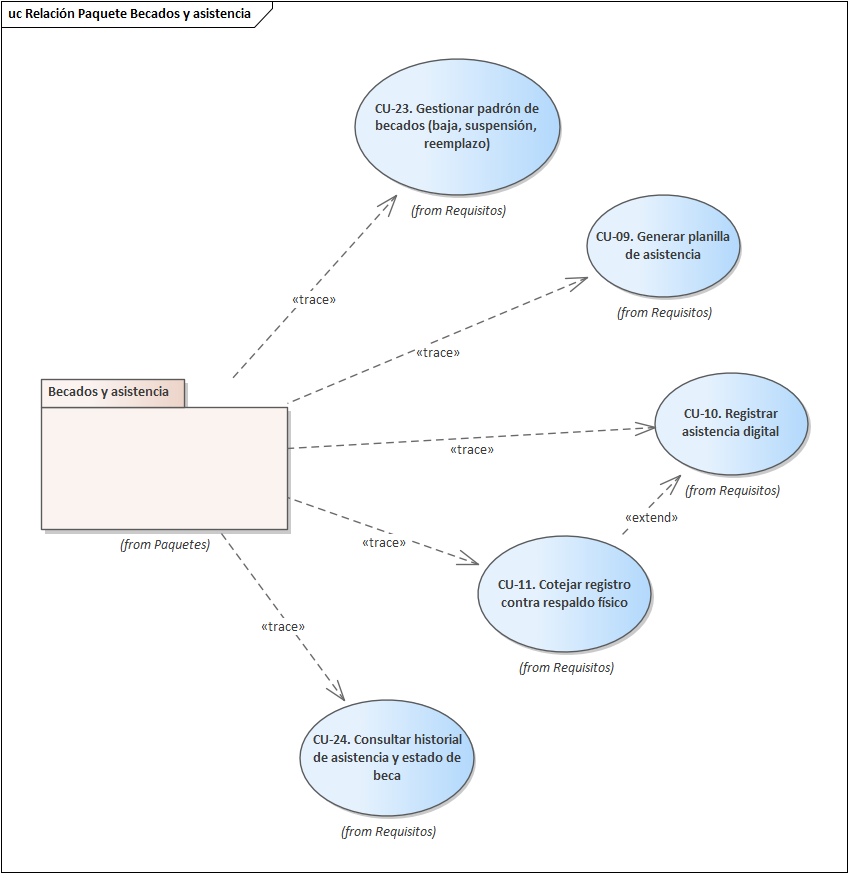
\includegraphics[width=\textwidth,height=0.85\textheight,keepaspectratio]{images/036_Relacion_Becados_Asistencia.png}

\smallskip
\noindent\raggedright\textit{Nota.} Elaboración propia.
\end{figure}

El paquete Reportes y Trazabilidad se relaciona con los casos de uso CU-12 y CU-25, como se muestra en la Figura~\ref{fig:rel_reportes}.

\begin{figure}[H]
\caption{Relación del paquete Reportes y Trazabilidad}
\label{fig:rel_reportes}
\centering
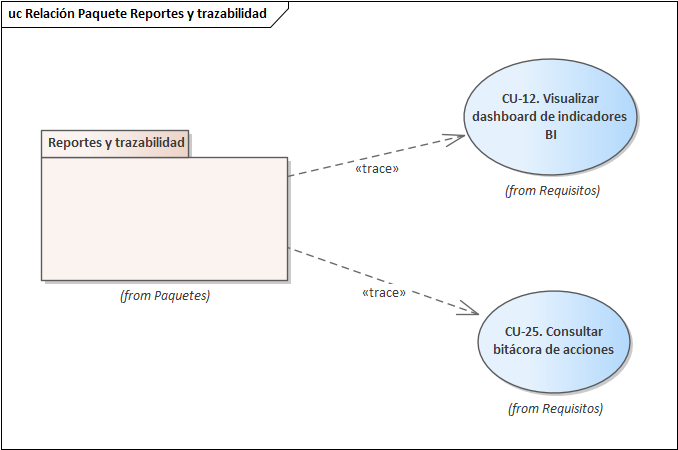
\includegraphics[width=\textwidth,height=0.85\textheight,keepaspectratio]{images/037_Relacion_Reportes_Trazabilidad.png}

\smallskip
\noindent\raggedright\textit{Nota.} Elaboración propia.
\end{figure}

\wfb{\wn{6}.1.3. Encapsulamiento de Casos de Uso por Paquetes}\label{sec:cap6_encapsulamiento_cu}

% [PENDIENTE]: Redactar la introducción del encapsulamiento (criterio de agrupación de los casos de uso).

Las Figuras~\ref{fig:enc_cuentas}, \ref{fig:enc_convocatoria}, \ref{fig:enc_preseleccion}, \ref{fig:enc_auditoria}, \ref{fig:enc_becados} y~\ref{fig:enc_reportes} muestran el encapsulamiento de los casos de uso en cada uno de los seis paquetes de análisis del sistema.

El paquete Cuentas y Acceso encapsula los casos de uso CU-01, CU-14 y CU-15, como se muestra en la Figura~\ref{fig:enc_cuentas}.

\begin{figure}[H]
\caption{Encapsulamiento de casos de uso del paquete Cuentas y Acceso}
\label{fig:enc_cuentas}
\centering
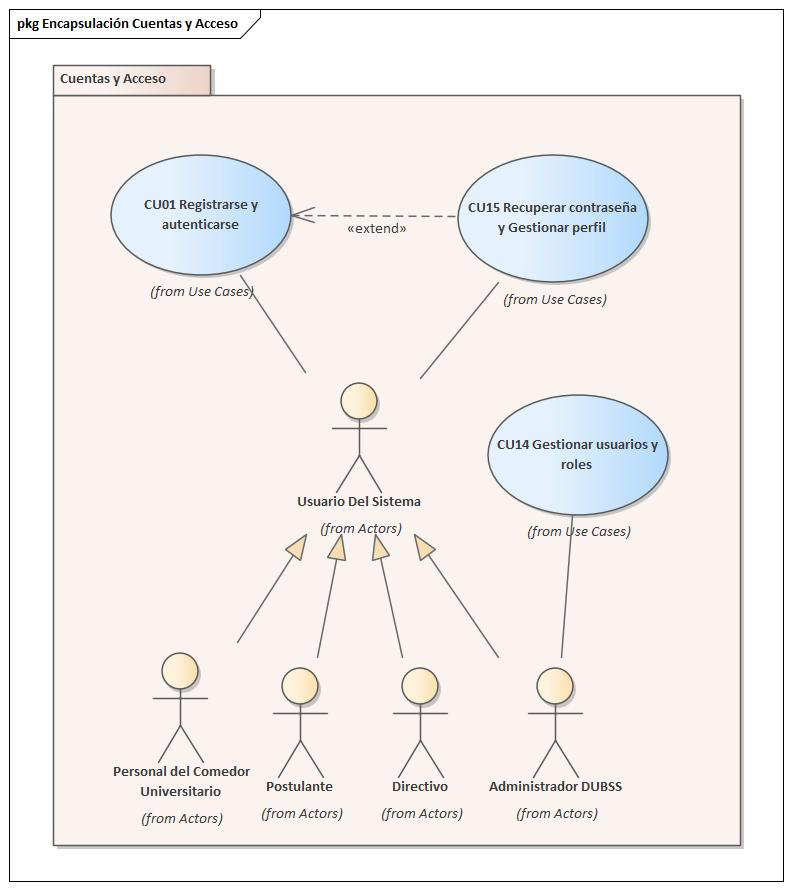
\includegraphics[width=\textwidth,height=0.85\textheight,keepaspectratio]{images/022_Encapsulamiento_Cuentas_Acceso.jpg}

\smallskip
\noindent\raggedright\textit{Nota.} Elaboración propia.
\end{figure}

El paquete Convocatoria y Postulación encapsula los casos de uso CU-02, CU-04, CU-13, CU-16, CU-17 y CU-18, como se muestra en la Figura~\ref{fig:enc_convocatoria}.

\begin{figure}[H]
\caption{Encapsulamiento de casos de uso del paquete Convocatoria y Postulación}
\label{fig:enc_convocatoria}
\centering
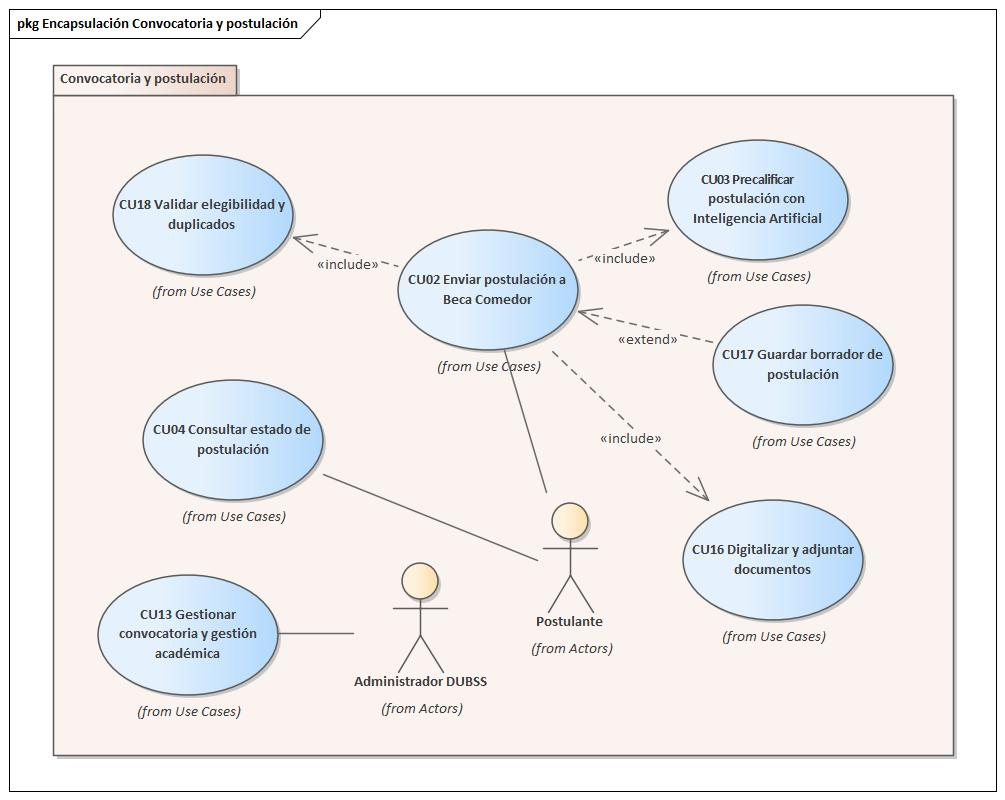
\includegraphics[width=\textwidth,height=0.85\textheight,keepaspectratio]{images/023_Encapsulamiento_Convocatoria_Postulacion.jpg}

\smallskip
\noindent\raggedright\textit{Nota.} Elaboración propia.
\end{figure}

El paquete Preselección con IA encapsula los casos de uso CU-03 y CU-26, como se muestra en la Figura~\ref{fig:enc_preseleccion}.

\begin{figure}[H]
\caption{Encapsulamiento de casos de uso del paquete Preselección con IA}
\label{fig:enc_preseleccion}
\centering
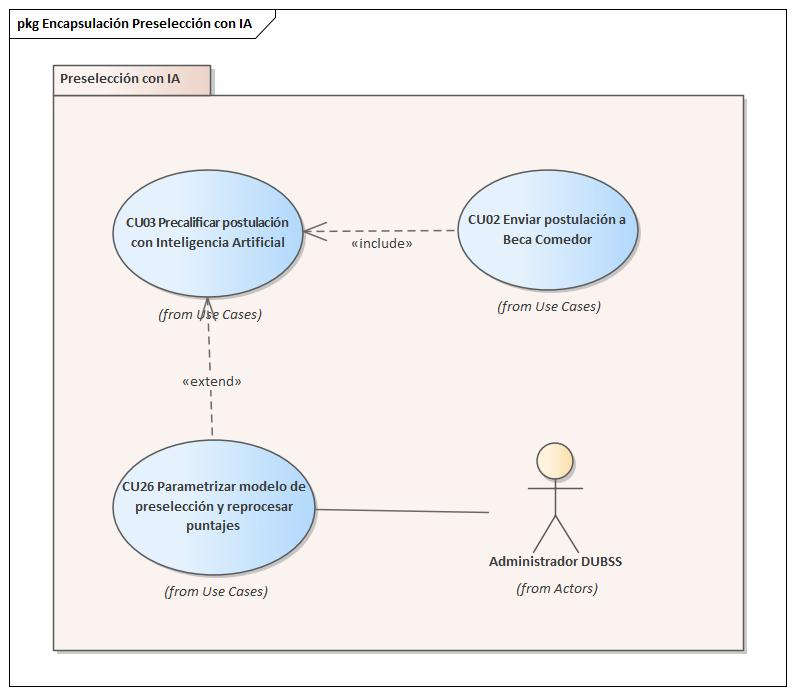
\includegraphics[width=\textwidth,height=0.85\textheight,keepaspectratio]{images/024_Encapsulamiento_Preseleccion_IA.jpg}

\smallskip
\noindent\raggedright\textit{Nota.} Elaboración propia.
\end{figure}

El paquete Auditoría y Adjudicación encapsula los casos de uso CU-05, CU-06, CU-07, CU-08, CU-19, CU-20, CU-21 y CU-22, como se muestra en la Figura~\ref{fig:enc_auditoria}.

\begin{figure}[H]
\caption{Encapsulamiento de casos de uso del paquete Auditoría y Adjudicación}
\label{fig:enc_auditoria}
\centering
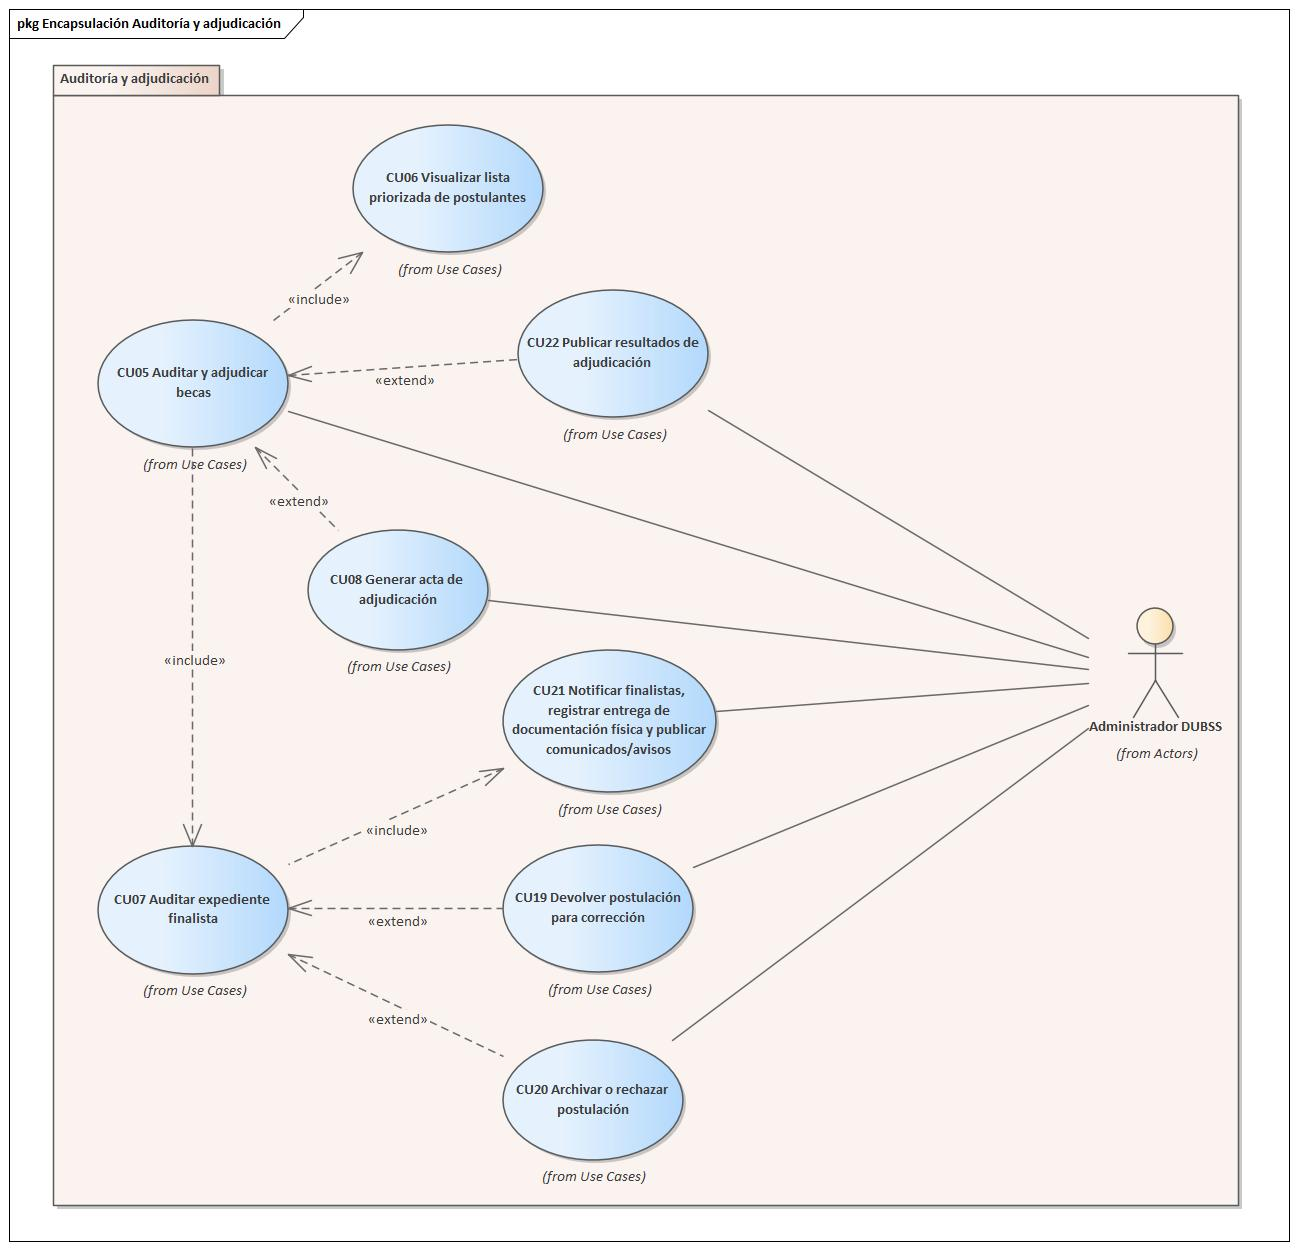
\includegraphics[width=\textwidth,height=0.85\textheight,keepaspectratio]{images/025_Encapsulamiento_Auditoria_Adjudicacion.jpg}

\smallskip
\noindent\raggedright\textit{Nota.} Elaboración propia.
\end{figure}

El paquete Becados y Asistencia encapsula los casos de uso CU-09, CU-10, CU-11, CU-23 y CU-24, como se muestra en la Figura~\ref{fig:enc_becados}.

\begin{figure}[H]
\caption{Encapsulamiento de casos de uso del paquete Becados y Asistencia}
\label{fig:enc_becados}
\centering
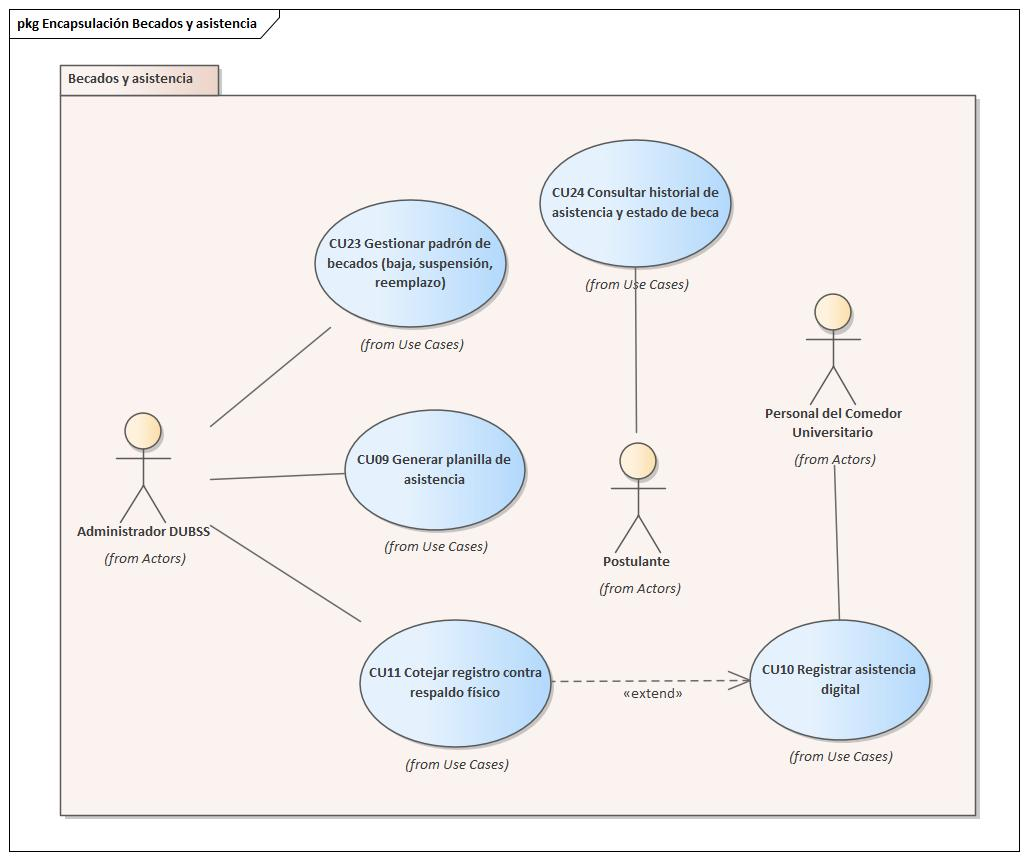
\includegraphics[width=\textwidth,height=0.85\textheight,keepaspectratio]{images/026_Encapsulamiento_Becados_Asistencia.jpg}

\smallskip
\noindent\raggedright\textit{Nota.} Elaboración propia.
\end{figure}

El paquete Reportes y Trazabilidad encapsula los casos de uso CU-12 y CU-25, como se muestra en la Figura~\ref{fig:enc_reportes}.

\begin{figure}[H]
\caption{Encapsulamiento de casos de uso del paquete Reportes y Trazabilidad}
\label{fig:enc_reportes}
\centering
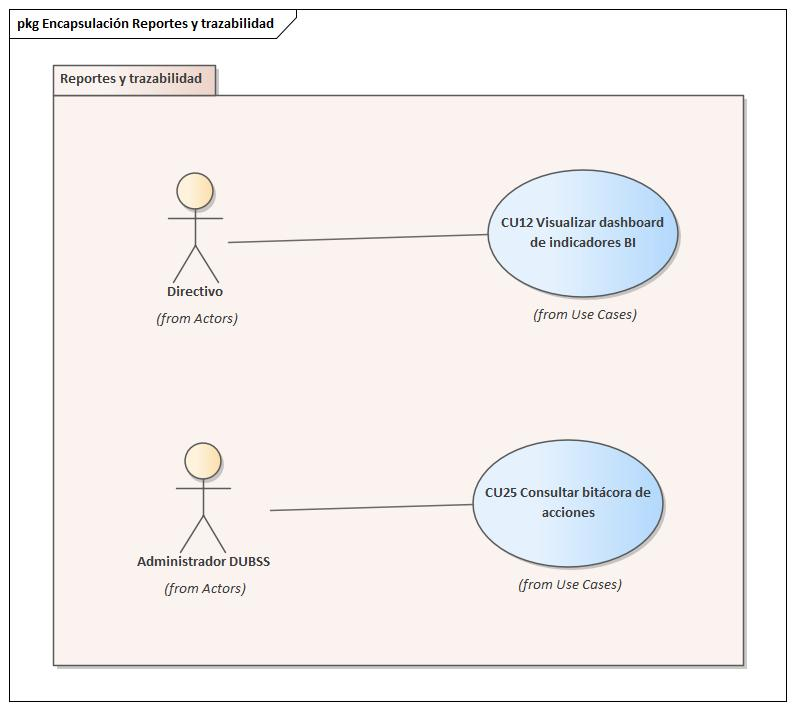
\includegraphics[width=\textwidth,height=0.85\textheight,keepaspectratio]{images/027_Encapsulamiento_Reportes_Trazabilidad.jpg}

\smallskip
\noindent\raggedright\textit{Nota.} Elaboración propia.
\end{figure}

% ------------------------------------------------------------------------------
% 6.2. ANÁLISIS DE CASOS DE USO
% ------------------------------------------------------------------------------
\subsection{6.2. Análisis de Casos de Uso}\label{sec:cap6_analisis_cu}

El análisis de cada caso de uso se realizó mediante diagramas de colaboración que representan las clases de análisis que intervienen y los mensajes que intercambian. Siguiendo el Proceso Unificado de Desarrollo de Software, el modelo de análisis distingue tres tipos de clases: las clases de interfaz (\textit{boundary}), que modelan la interacción del actor con el sistema; las clases de control (\textit{control}), que coordinan la lógica de cada caso de uso; y las clases de entidad (\textit{entity}), que representan la información persistente del dominio \parencite{jacobson1999unified}. Estos diagramas se expresan en el Lenguaje Unificado de Modelado \parencite{booch2005uml}.

En todos los diagramas, el actor se comunica con la interfaz (clase terminada en \textit{View}), esta con el controlador (clase terminada en \textit{Controller}) y el controlador con las entidades; no existe comunicación directa entre el actor y el controlador ni entre la interfaz y las entidades. Los mensajes se numeran jerárquicamente: el número entero corresponde a la operación que solicita el actor, y los subniveles (1.1, 1.2, etc.) a los mensajes que se derivan de ella hacia el controlador y las entidades. Las flechas se diferencian por color según el tipo de operación. Los nombres de las entidades se corresponden con las tablas del modelo de datos del sistema.

A continuación se presenta el análisis de los veintiséis casos de uso del sistema, en el orden de su numeración (CU-01 a CU-26).

\subsubsection{6.2.1. Analizar CU-01 Registrarse y autenticarse}\label{sec:cap6_analisis_cu01}

En el análisis del CU-01 participa el actor Usuario del Sistema, generalizado por los cuatro roles del sistema (Postulante, Administrador DUBSS, Directivo y Personal del Comedor Universitario), de modo que cualquiera de ellos puede iniciar y cerrar sesión (el registro corresponde únicamente al Postulante). El actor interactúa con la interfaz \textit{AuthView}, que delega las solicitudes en el controlador \textit{AuthController}, y este accede a las entidades \textit{Usuario}, \textit{Postulante}, \textit{Sesion} y \textit{Bitacora}. La verificación de las credenciales, la emisión de los tokens y el bloqueo por intentos fallidos los resuelve el propio sistema. La Figura~\ref{fig:analisis_cu01} presenta el diagrama de análisis.

\begin{figure}[H]
\caption{Análisis del CU-01 Registrarse y autenticarse}
\label{fig:analisis_cu01}
\centering
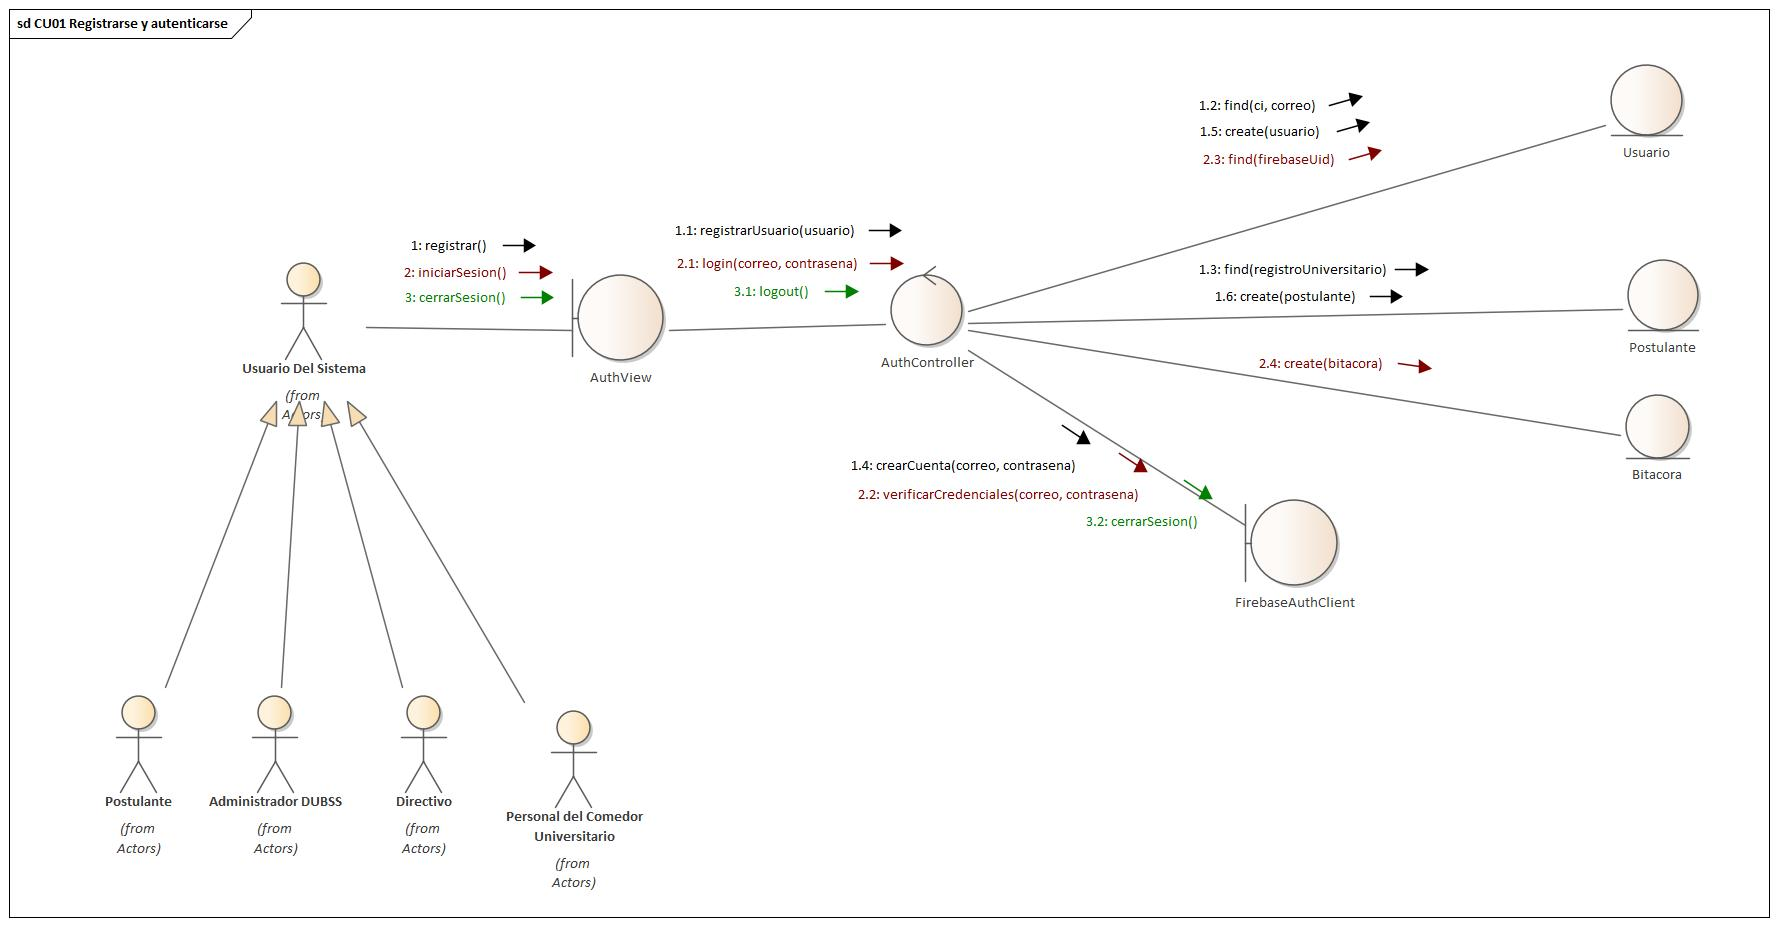
\includegraphics[width=\textwidth,height=0.5\textheight,keepaspectratio]{images/051_Analisis_CU01_Registrarse_Autenticarse.jpg}

\smallskip
\noindent\raggedright\textit{Nota.} Elaboración propia.
\end{figure}

El registro (mensaje 1) verifica que el CI, el registro universitario y el correo electrónico no existan (1.2 y 1.3), crea el usuario con la contraseña almacenada como hash (1.4) y, para el rol Postulante, su perfil (1.5), abre la sesión (1.6) y anota el registro en la bitácora (1.7). El inicio de sesión (mensaje 2) consulta al usuario por su correo electrónico (2.2) y verifica la contraseña; si es incorrecta, actualiza el contador de intentos fallidos y, de ser necesario, el bloqueo (2.3); si es correcta, crea la sesión (2.4) y anota el acceso en la bitácora (2.5). La renovación de la sesión (mensaje 3) busca la sesión por el hash de su token (3.2), la revoca (3.3) y crea una nueva (3.4), de modo que el token de renovación se reemplaza en cada uso. El cierre de sesión (mensaje 4) revoca la sesión del dispositivo desde el que se solicita (4.2). La consulta del usuario actual (mensaje 5) busca al usuario por su código público (5.2). De este modo, la contraseña y el token de renovación se almacenan solo como hash, nunca en texto plano.


\subsubsection{6.2.2. Analizar CU-02 Enviar postulación a Beca Comedor}\label{sec:cap6_analisis_cu02}

El CU-02 es iniciado por el Postulante a través de \textit{PostulacionView}, que se comunica con \textit{PostulacionController}. Este controlador utiliza las entidades \textit{Convocatoria}, \textit{Postulacion} y \textit{RespuestaSocioeconomica}. La digitalización de documentos, la validación de elegibilidad y la precalificación se resuelven en los casos de uso incluidos (CU-16, CU-18 y CU-03), por lo que no se repiten en este diagrama. La Figura~\ref{fig:analisis_cu02} presenta el diagrama de análisis.

\begin{figure}[H]
\caption{Análisis del CU-02 Enviar postulación a Beca Comedor}
\label{fig:analisis_cu02}
\centering
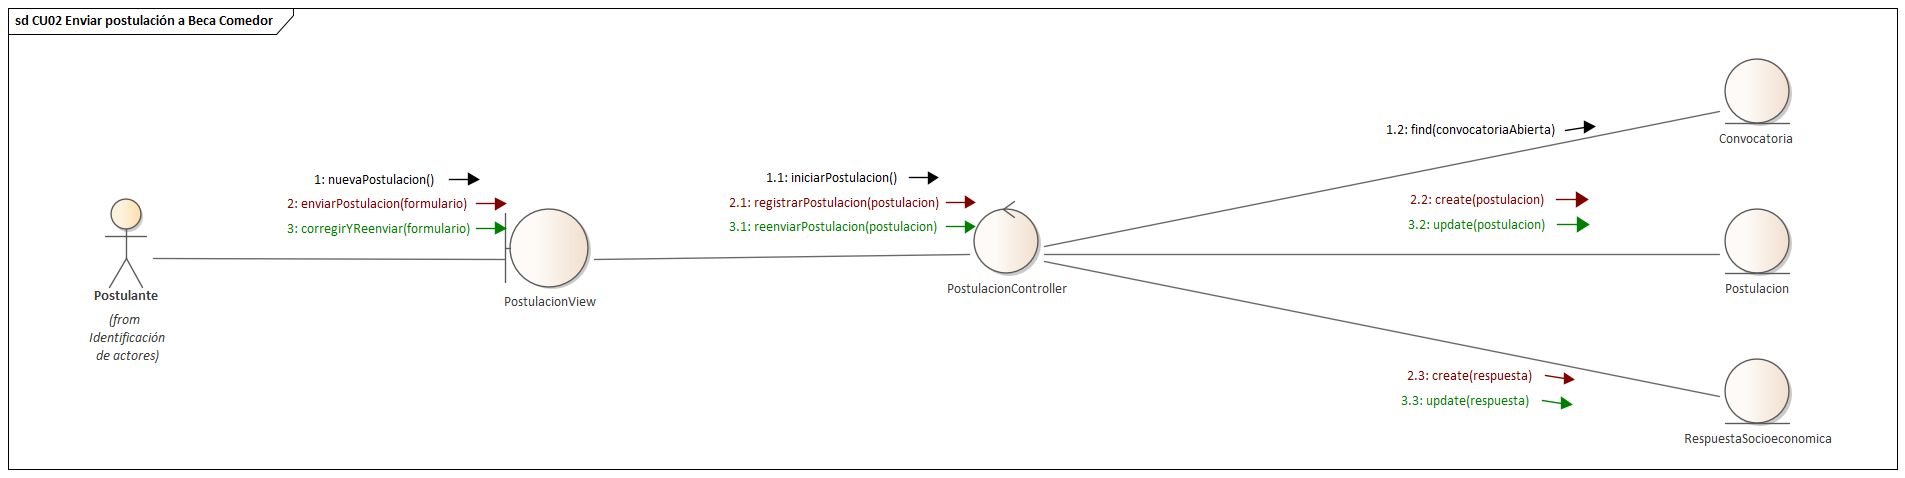
\includegraphics[width=\textwidth,height=0.5\textheight,keepaspectratio]{images/052_Analisis_CU02_Enviar_Postulacion_Beca_Comedor.png}

\smallskip
\noindent\raggedright\textit{Nota.} Elaboración propia.
\end{figure}

Al iniciar una nueva postulación (mensaje 1), el controlador consulta la convocatoria abierta (1.2). Al enviar el formulario (mensaje 2), crea la postulación (2.2) y su respuesta socioeconómica (2.3). Si la postulación fue devuelta para corrección, el Postulante la corrige y la reenvía (mensaje 3), con lo cual se actualizan la postulación (3.2) y la respuesta socioeconómica (3.3) sobre los mismos registros.


\subsubsection{6.2.3. Analizar CU-03 Precalificar postulación con Inteligencia Artificial}\label{sec:cap6_analisis_cu03}

El CU-03 se dispara cuando el Postulante envía su postulación desde \textit{PostulacionView}. El controlador \textit{PrecalificacionController} recibe la solicitud de precalificación y colabora con las entidades \textit{Postulacion}, \textit{ModeloPreseleccion}, \textit{ParametroModelo} y \textit{PuntajePostulacion}. El módulo de Inteligencia Artificial no se representa como objeto independiente: su ejecución se modela como el mensaje 1.5 del propio controlador. La Figura~\ref{fig:analisis_cu03} presenta el diagrama de análisis.

\begin{figure}[H]
\caption{Análisis del CU-03 Precalificar postulación con Inteligencia Artificial}
\label{fig:analisis_cu03}
\centering
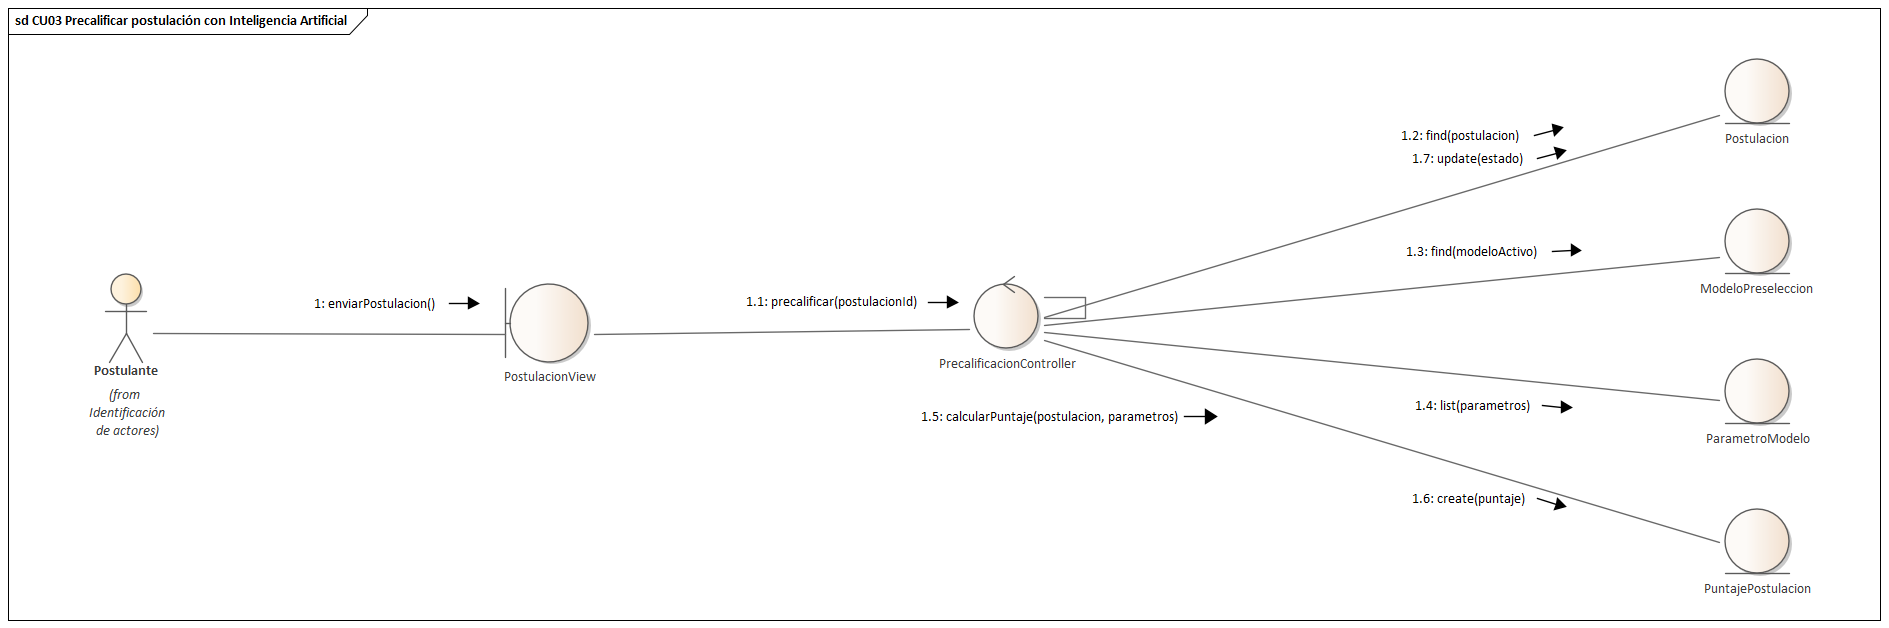
\includegraphics[width=\textwidth,height=0.5\textheight,keepaspectratio]{images/053_Analisis_CU03_Precalificar_Postulacion_IA.png}

\smallskip
\noindent\raggedright\textit{Nota.} Elaboración propia.
\end{figure}

El controlador obtiene la postulación (1.2), el modelo de preselección activo (1.3) y sus parámetros (1.4); calcula el puntaje de vulnerabilidad (1.5); registra el puntaje con su fecha de cálculo (1.6) y actualiza el estado de la postulación (1.7), lo que permite conservar la trazabilidad de cada cálculo.


\subsubsection{6.2.4. Analizar CU-04 Consultar estado de postulación}\label{sec:cap6_analisis_cu04}

En el CU-04, el Postulante consulta sus postulaciones mediante \textit{EstadoPostulacionView}, que se apoya en \textit{EstadoPostulacionController}. Las entidades involucradas son \textit{Postulacion} y \textit{PostulacionHistorial}. La Figura~\ref{fig:analisis_cu04} presenta el diagrama de análisis.

\begin{figure}[H]
\caption{Análisis del CU-04 Consultar estado de postulación}
\label{fig:analisis_cu04}
\centering
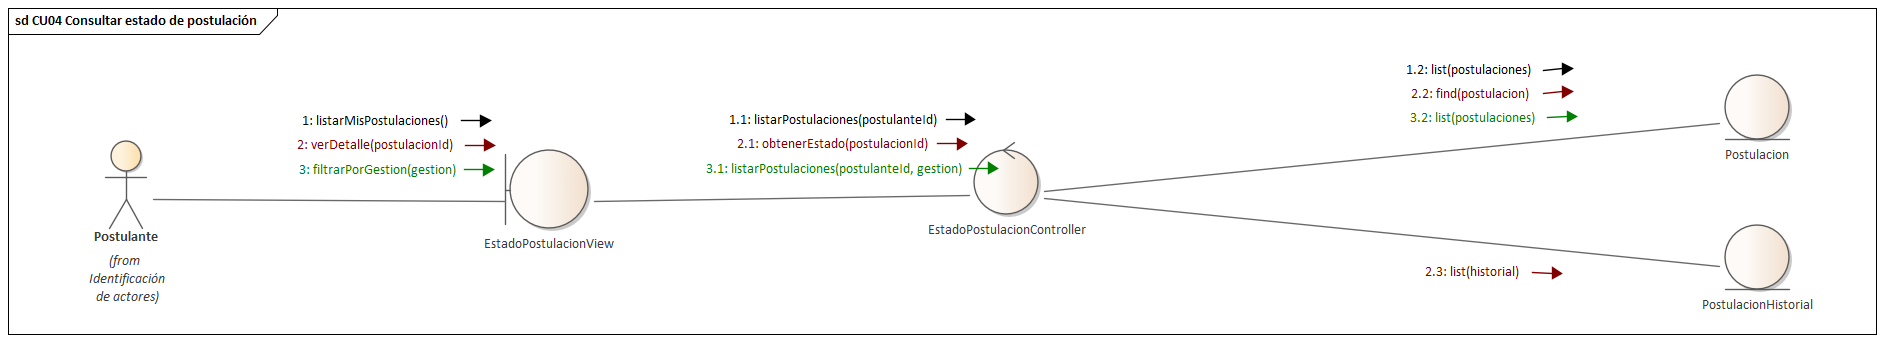
\includegraphics[width=\textwidth,height=0.5\textheight,keepaspectratio]{images/054_Analisis_CU04_Consultar_Estado_Postulacion.png}

\smallskip
\noindent\raggedright\textit{Nota.} Elaboración propia.
\end{figure}

El actor puede listar sus postulaciones (mensaje 1), ver el detalle de una de ellas (mensaje 2), lo que implica obtener la postulación (2.2) y su historial de cambios de estado (2.3), y filtrar las postulaciones por gestión académica (mensaje 3). Se trata de operaciones de solo lectura.


\subsubsection{6.2.5. Analizar CU-05 Auditar y adjudicar becas}\label{sec:cap6_analisis_cu05}

En el CU-05, el Administrador DUBSS conduce la adjudicación mediante \textit{AdjudicacionView}, que delega en \textit{AdjudicacionController}. Este controlador trabaja con las entidades \textit{Finalista}, \textit{Postulacion}, \textit{Adjudicacion} y \textit{PostulacionHistorial}: consulta los totales para el panel, selecciona finalistas según el orden de la lista priorizada y, al decidir, cambia el estado de la postulación, crea la adjudicación y deja la fila en el historial. La visualización de la lista priorizada y la auditoría de cada expediente se resuelven en los casos de uso incluidos (CU-06 y CU-07), por lo que no se repiten en este diagrama. La Figura~\ref{fig:analisis_cu05} presenta el diagrama de análisis.

\begin{figure}[H]
\caption{Análisis del CU-05 Auditar y adjudicar becas}
\label{fig:analisis_cu05}
\centering
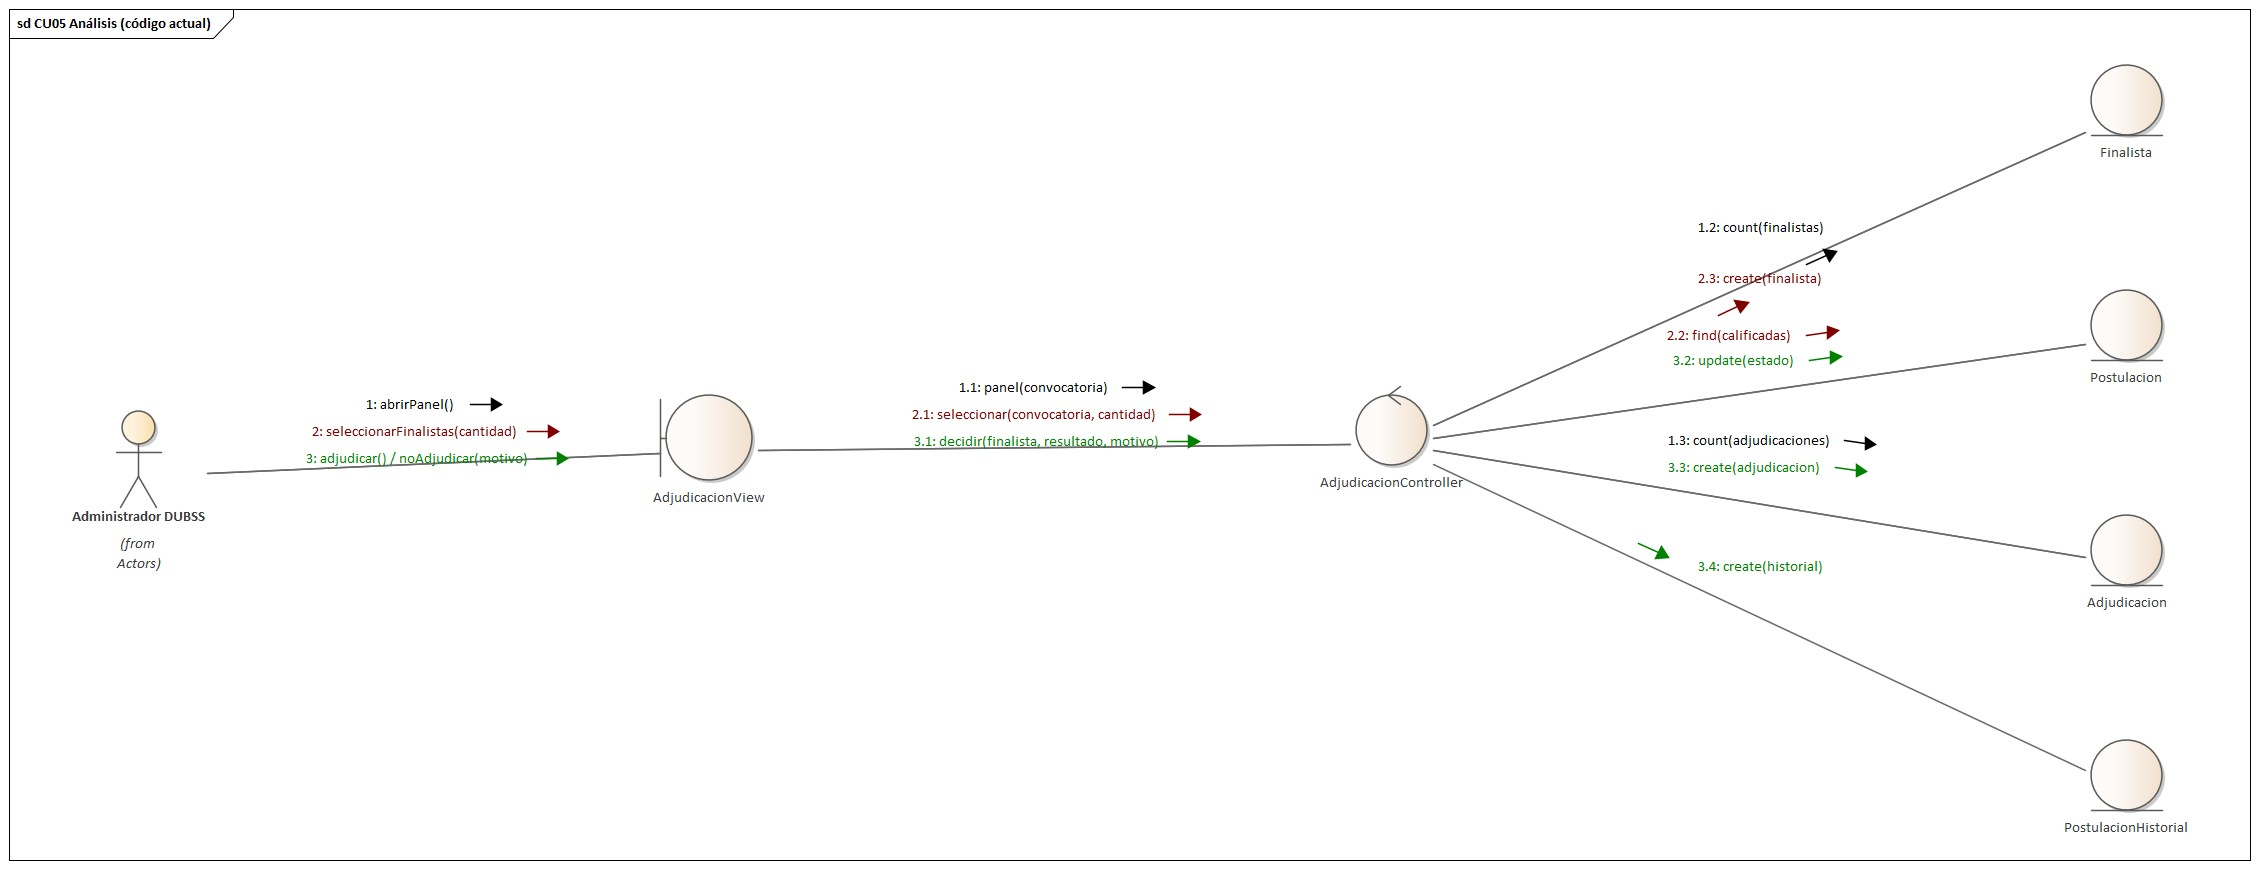
\includegraphics[width=\textwidth,height=0.5\textheight,keepaspectratio]{images/077_Analisis_CU05_Auditar_Adjudicar_Becas.jpg}

\smallskip
\noindent\raggedright\textit{Nota.} Elaboración propia.
\end{figure}

El Administrador puede listar los finalistas de la convocatoria (mensaje 1), con lo que el controlador obtiene los finalistas registrados (1.2). Al adjudicar una beca (mensaje 2), el controlador registra la decisión (2.1), crea la adjudicación con su resultado (2.2) y actualiza el estado de la postulación a «adjudicada» o «no adjudicada» (2.3).


\subsubsection{6.2.6. Analizar CU-06 Visualizar lista priorizada de postulantes}\label{sec:cap6_analisis_cu06}

En el CU-06, el Administrador DUBSS consulta la lista priorizada mediante \textit{ListaPriorizadaView}, que se comunica con \textit{PriorizacionController}. Las entidades involucradas son \textit{Postulacion} y \textit{PuntajePostulacion}; la lista no se almacena, sino que se obtiene a partir de ambas. Para la exportación a PDF interviene además \textit{Bitacora}, donde se registra la acción. La Figura~\ref{fig:analisis_cu06} presenta el diagrama de análisis.

\begin{figure}[H]
\caption{Análisis del CU-06 Visualizar lista priorizada de postulantes}
\label{fig:analisis_cu06}
\centering
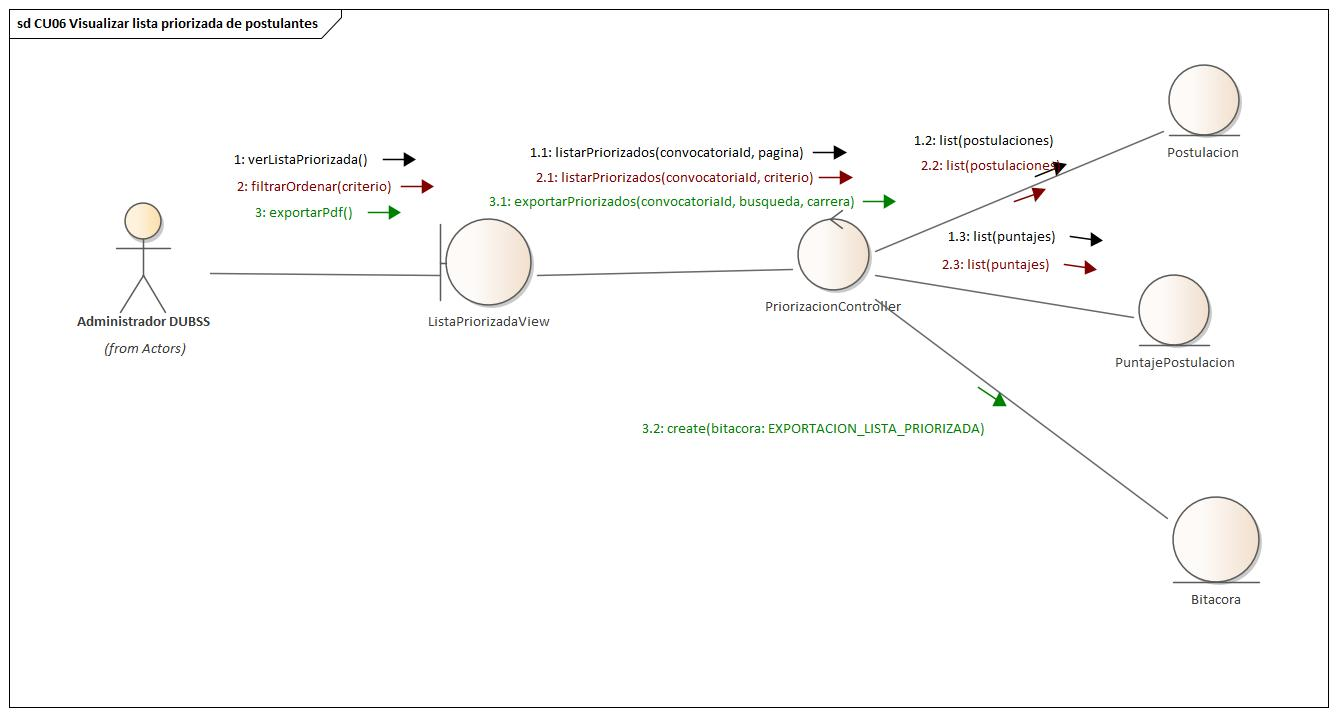
\includegraphics[width=\textwidth,height=0.5\textheight,keepaspectratio]{images/078_Analisis_CU06_Visualizar_Lista_Priorizada_Postulantes.jpg}

\smallskip
\noindent\raggedright\textit{Nota.} Elaboración propia.
\end{figure}

Al ver la lista priorizada (mensaje 1), el controlador solicita la página correspondiente de la convocatoria (1.1), obtiene las postulaciones calificadas (1.2) y sus puntajes vigentes (1.3), y las ordena de mayor a menor puntaje. Al filtrar u ordenar la lista (mensaje 2), se repite la consulta con el criterio indicado (2.1 a 2.3). Ambas operaciones son de solo lectura. Al exportar la lista (mensaje 3), el controlador recibe la solicitud con la convocatoria y los criterios de búsqueda y carrera vigentes (3.1), genera el documento PDF y registra la exportación en la bitácora con la acción EXPORTACION\_LISTA\_PRIORIZADA (3.2).


\subsubsection{6.2.7. Analizar CU-07 Auditar expediente finalista}\label{sec:cap6_analisis_cu07}

En el CU-07, el Administrador DUBSS revisa el expediente de un finalista mediante \textit{ExpedienteView} y \textit{ExpedienteController}, que colaboran con las entidades \textit{Finalista}, \textit{DocumentoAdjunto}, \textit{PuntajePostulacion}, \textit{AuditoriaExpediente}, \textit{Bitacora} y \textit{Notificacion}. La notificación al finalista y el registro de la entrega física se resuelven en el CU-21, incluido por este caso de uso. La Figura~\ref{fig:analisis_cu07} presenta el diagrama de análisis.

\begin{figure}[H]
\caption{Análisis del CU-07 Auditar expediente finalista}
\label{fig:analisis_cu07}
\centering
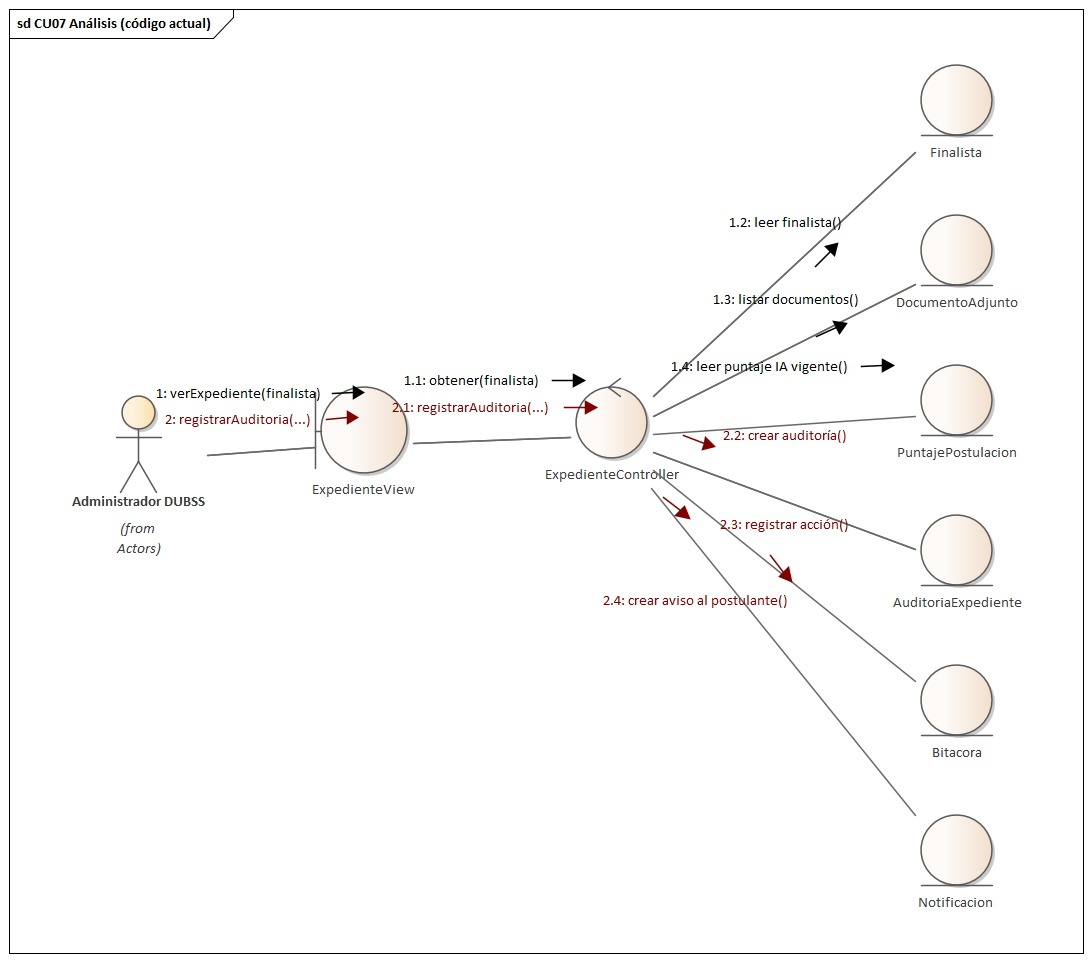
\includegraphics[width=\textwidth,height=0.5\textheight,keepaspectratio]{images/079_Analisis_CU07_Auditar_Expediente_Finalista.jpg}

\smallskip
\noindent\raggedright\textit{Nota.} Elaboración propia.
\end{figure}

Al ver el expediente (mensaje 1), el controlador obtiene el finalista (1.2) y la lista de sus documentos adjuntos (1.3) y el puntaje vigente de la inteligencia artificial para mostrar el total. Al registrar la auditoría (mensaje 2), el controlador recibe el resultado, las observaciones (hasta 500 caracteres) y el puntaje académico (0 a 30), y crea el registro de auditoría conservando las auditorías anteriores del expediente; luego deja constancia en la bitácora y crea la notificación que avisa el resultado al postulante.


\subsubsection{6.2.8. Analizar CU-08 Generar acta de adjudicación}\label{sec:cap6_analisis_cu08}

En el CU-08, el Administrador DUBSS genera el acta mediante \textit{ActaView} y \textit{ActaController}, que utiliza las entidades \textit{Adjudicacion} y \textit{ActaAdjudicacion}. La generación del documento PDF se modela como un mensaje del propio controlador (1.3). La Figura~\ref{fig:analisis_cu08} presenta el diagrama de análisis.

\begin{figure}[H]
\caption{Análisis del CU-08 Generar acta de adjudicación}
\label{fig:analisis_cu08}
\centering
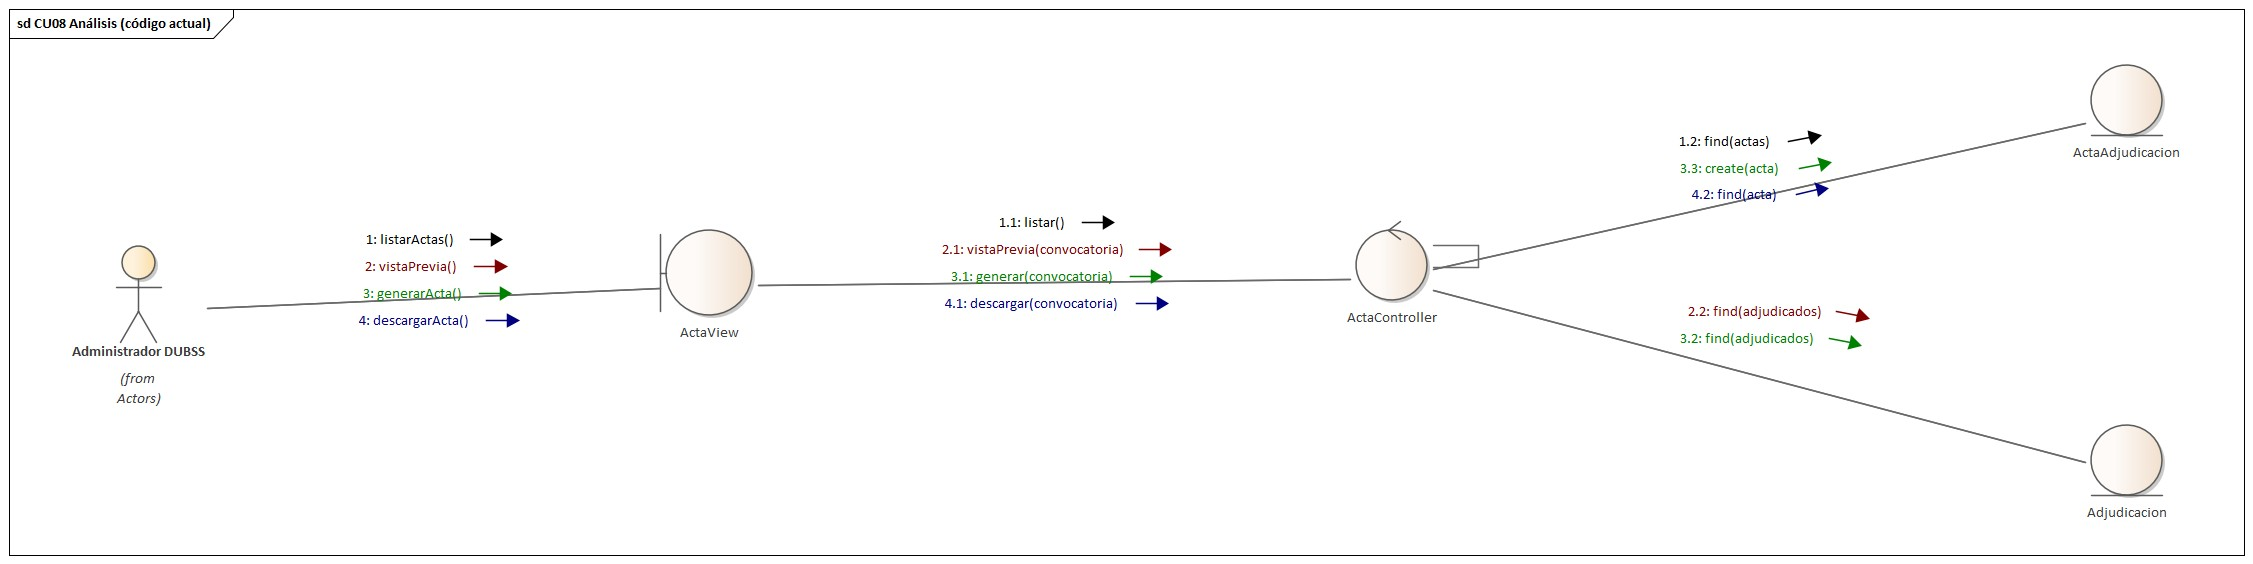
\includegraphics[width=\textwidth,height=0.5\textheight,keepaspectratio]{images/080_Analisis_CU08_Generar_Acta_Adjudicacion.jpg}

\smallskip
\noindent\raggedright\textit{Nota.} Elaboración propia.
\end{figure}

Al generar el acta (mensaje 1), el controlador obtiene las adjudicaciones de la convocatoria (1.2), genera el documento PDF (1.3) y crea el registro del acta (1.4). Al consultar el acta (mensaje 2), el controlador obtiene el acta registrada de la convocatoria (2.2).


\subsubsection{6.2.9. Analizar CU-09 Generar planilla de asistencia}\label{sec:cap6_analisis_cu09}

En el CU-09, el Administrador DUBSS genera las planillas mediante \textit{PlanillaView} y \textit{PlanillaController}, que trabajan con las entidades \textit{Beca} y \textit{PlanillaAsistencia}. La generación del documento PDF imprimible se modela como un mensaje del propio controlador (1.3). La Figura~\ref{fig:analisis_cu09} presenta el diagrama de análisis.

\begin{figure}[H]
\caption{Análisis del CU-09 Generar planilla de asistencia}
\label{fig:analisis_cu09}
\centering
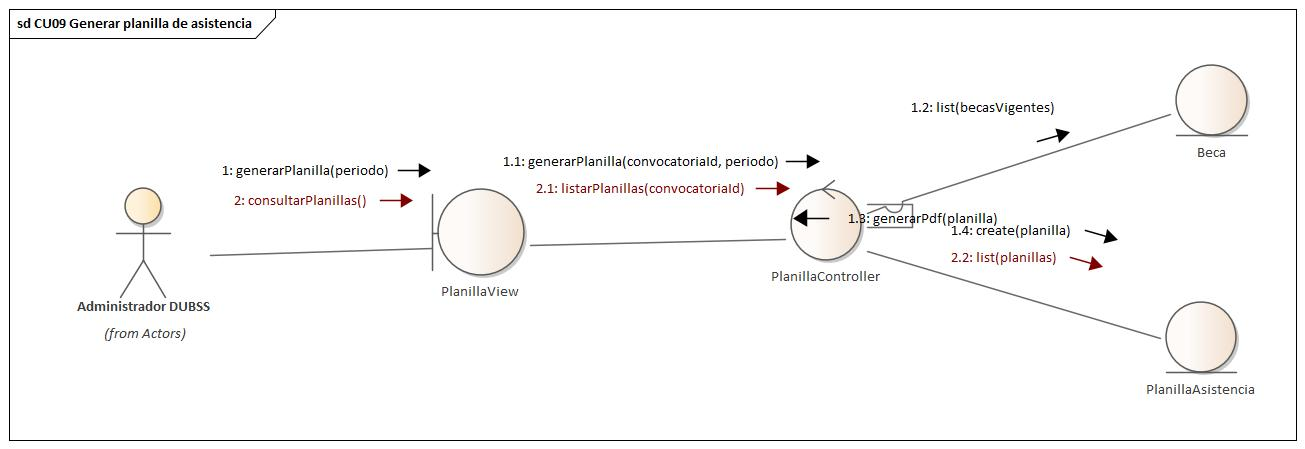
\includegraphics[width=\textwidth,height=0.5\textheight,keepaspectratio]{images/081_Analisis_CU09_Generar_Planilla_Asistencia.jpg}

\smallskip
\noindent\raggedright\textit{Nota.} Elaboración propia.
\end{figure}

Al generar una planilla para un periodo (mensaje 1), el controlador obtiene las becas vigentes de la convocatoria (1.2), genera el PDF con los espacios de firma y fotocopia de carnet (1.3) y crea el registro de la planilla (1.4). Al consultar las planillas (mensaje 2), el controlador lista las planillas generadas para la convocatoria (2.2).


\subsubsection{6.2.10. Analizar CU-10 Registrar asistencia digital}\label{sec:cap6_analisis_cu10}

En el CU-10, el Personal del Comedor Universitario registra la asistencia desde la aplicación móvil mediante \textit{RegistrarAsistenciaView}, que delega en \textit{AsistenciaControllerMobile}. Las entidades involucradas son \textit{Beca} y \textit{Asistencia}. La Figura~\ref{fig:analisis_cu10} presenta el diagrama de análisis.

\begin{figure}[H]
\caption{Análisis del CU-10 Registrar asistencia digital}
\label{fig:analisis_cu10}
\centering
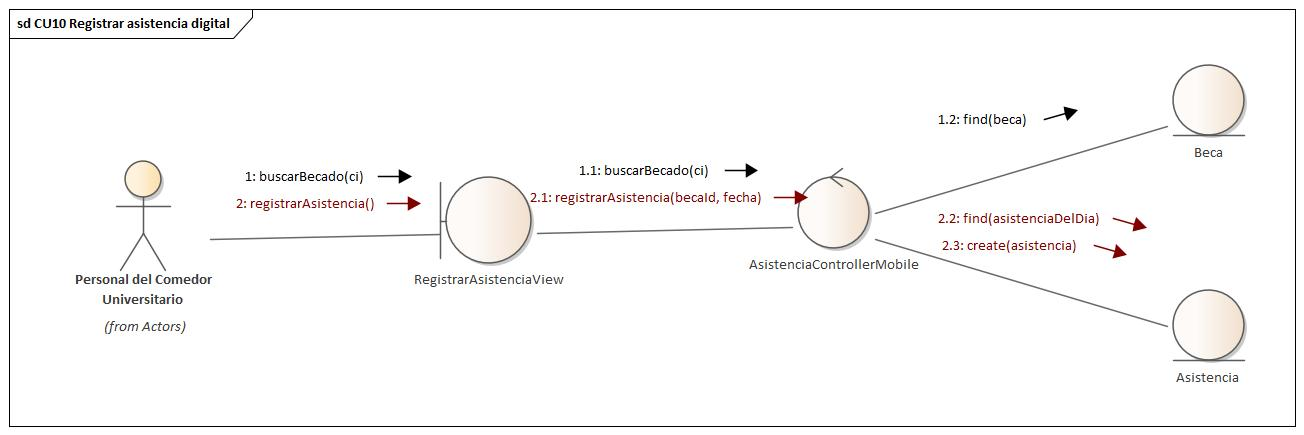
\includegraphics[width=\textwidth,height=0.5\textheight,keepaspectratio]{images/082_Analisis_CU10_Registrar_Asistencia_Digital.jpg}

\smallskip
\noindent\raggedright\textit{Nota.} Elaboración propia.
\end{figure}

Al buscar al becado por su CI (mensaje 1), el controlador obtiene su beca (1.2) para verificar que esté vigente. Al registrar la asistencia (mensaje 2), el controlador verifica si ya existe una asistencia de esa beca en el día (2.2) y, si no existe, crea el registro de asistencia (2.3); de este modo, una petición duplicada no genera un segundo registro.


\subsubsection{6.2.11. Analizar CU-11 Cotejar registro contra respaldo físico}\label{sec:cap6_analisis_cu11}

En el CU-11, el Administrador DUBSS realiza el cotejo mediante \textit{CotejoView} y \textit{CotejoController}, que colaboran con las entidades \textit{PlanillaAsistencia}, \textit{Asistencia} y \textit{CotejoAsistencia}. La Figura~\ref{fig:analisis_cu11} presenta el diagrama de análisis.

\begin{figure}[H]
\caption{Análisis del CU-11 Cotejar registro contra respaldo físico}
\label{fig:analisis_cu11}
\centering
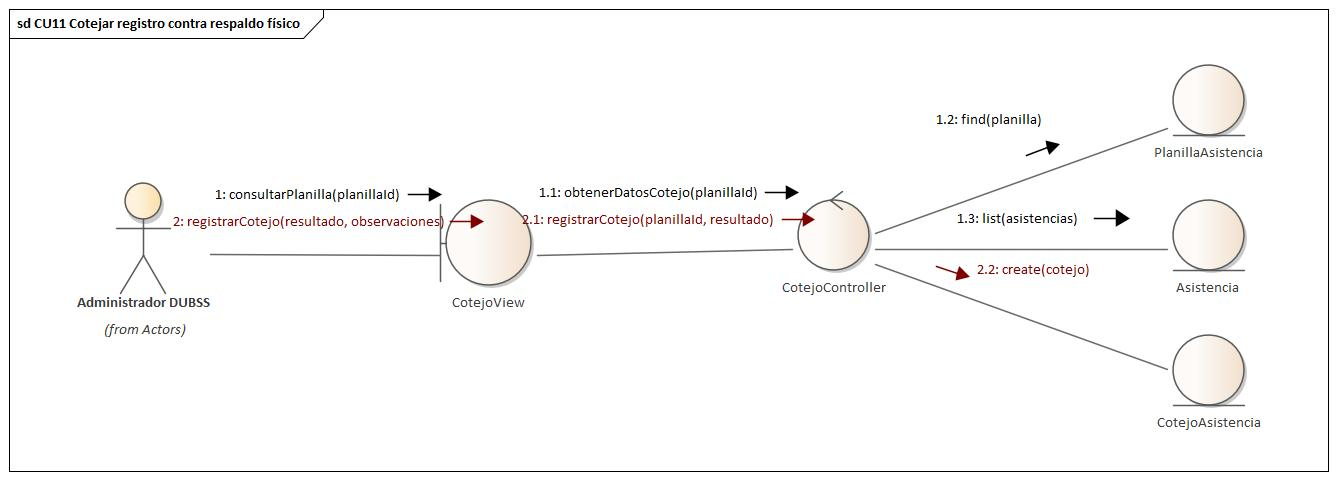
\includegraphics[width=\textwidth,height=0.5\textheight,keepaspectratio]{images/083_Analisis_CU11_Cotejar_Registro_Respaldo_Fisico.jpg}

\smallskip
\noindent\raggedright\textit{Nota.} Elaboración propia.
\end{figure}

Al consultar una planilla (mensaje 1), el controlador obtiene la planilla (1.2) y la lista de asistencias registradas en su periodo (1.3). Al registrar el cotejo (mensaje 2), el controlador recibe el resultado (2.1) y crea el registro del cotejo (2.2), sin modificar los registros de asistencia.


\subsubsection{6.2.12. Analizar CU-12 Visualizar dashboard de indicadores BI}\label{sec:cap6_analisis_cu12}

En el CU-12, el Directivo consulta el dashboard mediante \textit{DashboardView} y \textit{DashboardController}. La única entidad involucrada es \textit{IndicadoresConvocatoria}, que representa los indicadores precalculados por lotes a partir de las postulaciones, adjudicaciones, becas y asistencias. La Figura~\ref{fig:analisis_cu12} presenta el diagrama de análisis.

\begin{figure}[H]
\caption{Análisis del CU-12 Visualizar dashboard de indicadores BI}
\label{fig:analisis_cu12}
\centering
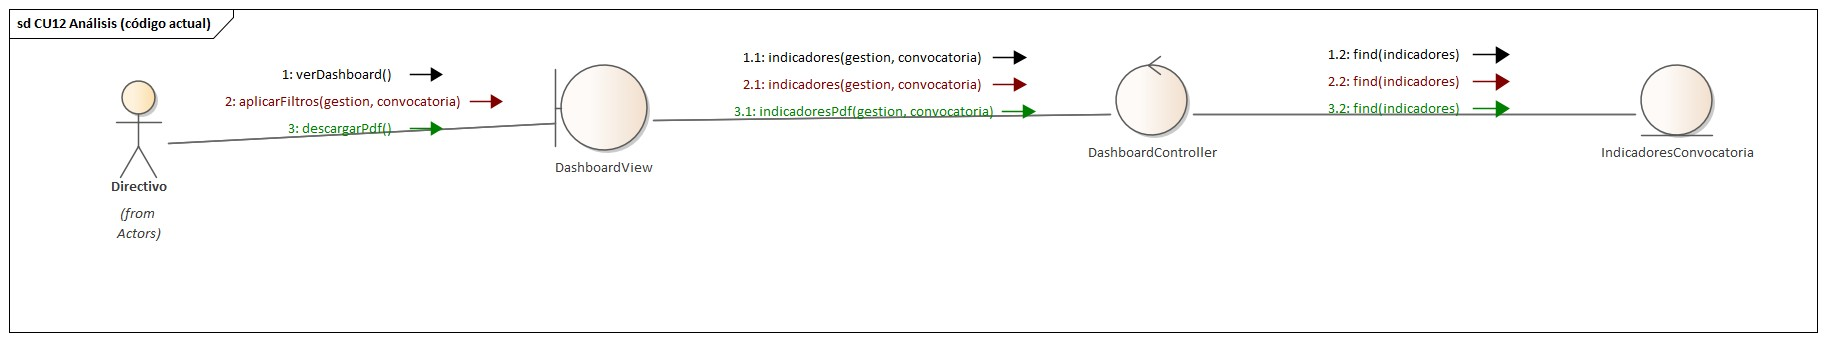
\includegraphics[width=\textwidth,height=0.5\textheight,keepaspectratio]{images/084_Analisis_CU12_Visualizar_Dashboard_Indicadores_BI.jpg}

\smallskip
\noindent\raggedright\textit{Nota.} Elaboración propia.
\end{figure}

Al ver los indicadores (mensaje 1), el controlador los consulta para la gestión académica vigente (1.1) y obtiene la lista de indicadores (1.2). Al filtrar por gestión (mensaje 2), se repite la consulta con la gestión y los filtros seleccionados (2.1 y 2.2). Ambas operaciones son de solo lectura.


\subsubsection{6.2.13. Analizar CU-13 Gestionar convocatoria y gestión académica}\label{sec:cap6_analisis_cu13}

En el CU-13, el Administrador DUBSS gestiona las convocatorias mediante \textit{ConvocatoriaView} y \textit{ConvocatoriaController}, que trabajan con las entidades \textit{Convocatoria}, \textit{GestionAcademica} y \textit{ConvocatoriaDocumento}. La Figura~\ref{fig:analisis_cu13} presenta el diagrama de análisis.

\begin{figure}[H]
\caption{Análisis del CU-13 Gestionar convocatoria y gestión académica}
\label{fig:analisis_cu13}
\centering
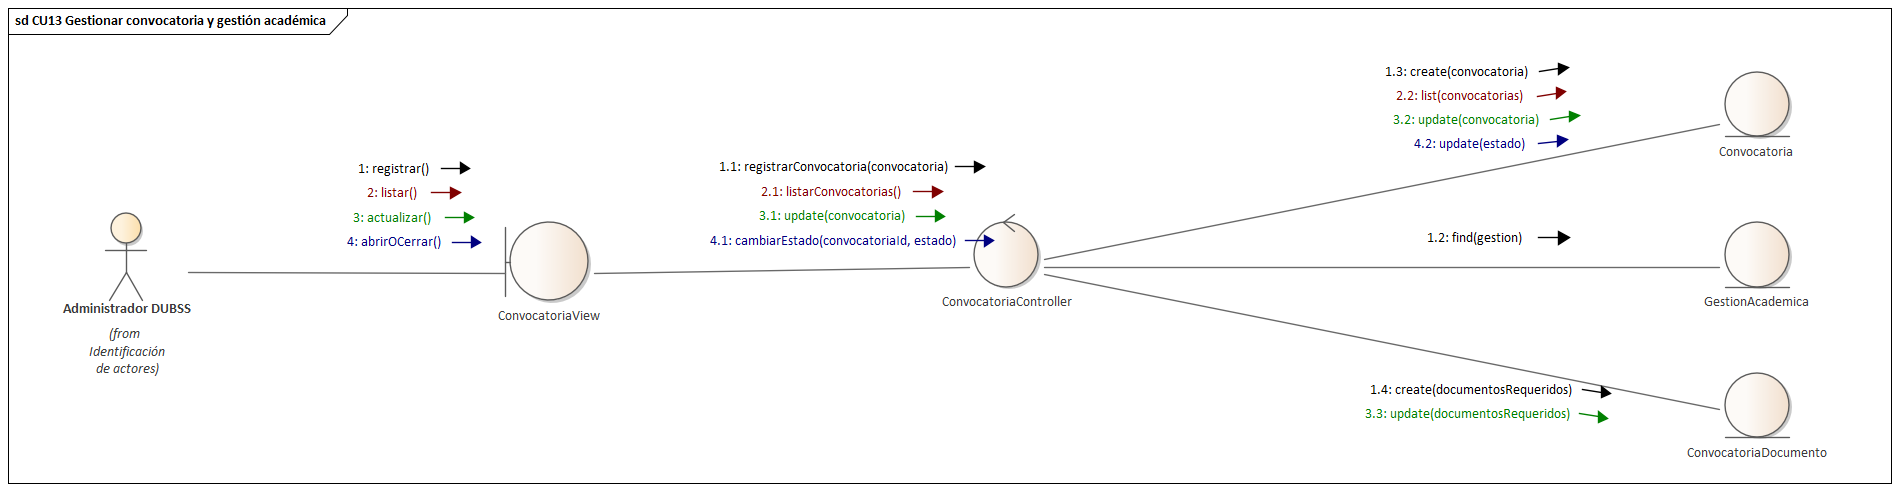
\includegraphics[width=\textwidth,height=0.5\textheight,keepaspectratio]{images/055_Analisis_CU13_Gestionar_Convocatoria_Gestion_Academica.png}

\smallskip
\noindent\raggedright\textit{Nota.} Elaboración propia.
\end{figure}

El registro de una convocatoria (mensaje 1) consulta la gestión académica (1.2), crea la convocatoria (1.3) y crea la lista de documentos requeridos (1.4). El listado (mensaje 2) recupera las convocatorias (2.2). La actualización (mensaje 3) modifica la convocatoria (3.2) y sus documentos requeridos (3.3). Finalmente, abrir o cerrar una convocatoria (mensaje 4) actualiza su estado (4.2). No se incluye una operación de eliminación, pues una convocatoria con postulaciones asociadas solo puede cerrarse.


\subsubsection{6.2.14. Analizar CU-14 Gestionar usuarios y roles}\label{sec:cap6_analisis_cu14}

En el CU-14, el Administrador DUBSS administra las cuentas del personal mediante \textit{UsuarioView} y \textit{UsuarioController}, que utilizan las entidades \textit{Usuario} y \textit{Rol}. La Figura~\ref{fig:analisis_cu14} presenta el diagrama de análisis.

\begin{figure}[H]
\caption{Análisis del CU-14 Gestionar usuarios y roles}
\label{fig:analisis_cu14}
\centering
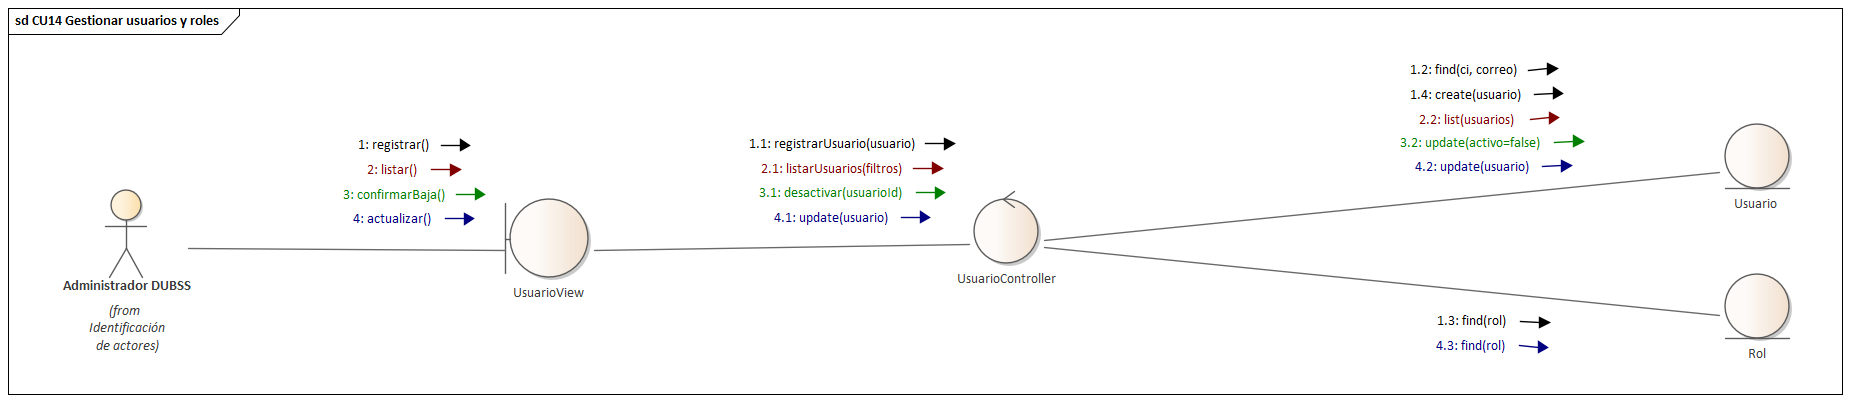
\includegraphics[width=\textwidth,height=0.5\textheight,keepaspectratio]{images/056_Analisis_CU14_Gestionar_Usuarios_Roles.png}

\smallskip
\noindent\raggedright\textit{Nota.} Elaboración propia.
\end{figure}

Para registrar una cuenta (mensaje 1), el controlador verifica que el CI y el correo no existan (1.2), consulta el rol asignado (1.3) y crea el usuario (1.4). El listado (mensaje 2) recupera los usuarios según los filtros indicados (2.2). La baja (mensaje 3) desactiva la cuenta mediante la actualización del campo de actividad (3.2), sin eliminar el registro, de modo que se preserve la trazabilidad. La actualización (mensaje 4) modifica los datos del usuario (4.2) y su rol (4.3).


\subsubsection{6.2.15. Analizar CU-15 Recuperar contraseña / gestionar perfil}\label{sec:cap6_analisis_cu15}

En el CU-15 participa el actor Usuario del Sistema, generalizado por los cuatro roles, quien interactúa con las vistas \textit{RecuperarContrasenaView} y \textit{PerfilView}. El controlador \textit{AuthController} atiende la recuperación, el restablecimiento y el cambio de contraseña, y \textit{PerfilController} la consulta y actualización del perfil; ambos colaboran con las entidades \textit{Usuario}, \textit{Postulante}, \textit{Sesion} y \textit{Bitacora}, y el envío del enlace pasa por la interfaz \textit{ServicioCorreo}. El enlace de restablecimiento no es una entidad aparte: su hash y su vencimiento se guardan en \textit{Usuario}, con un solo enlace vigente por cuenta. La Figura~\ref{fig:analisis_cu15} presenta el diagrama de análisis.

\begin{figure}[H]
\caption{Análisis del CU-15 Recuperar contraseña / gestionar perfil}
\label{fig:analisis_cu15}
\centering
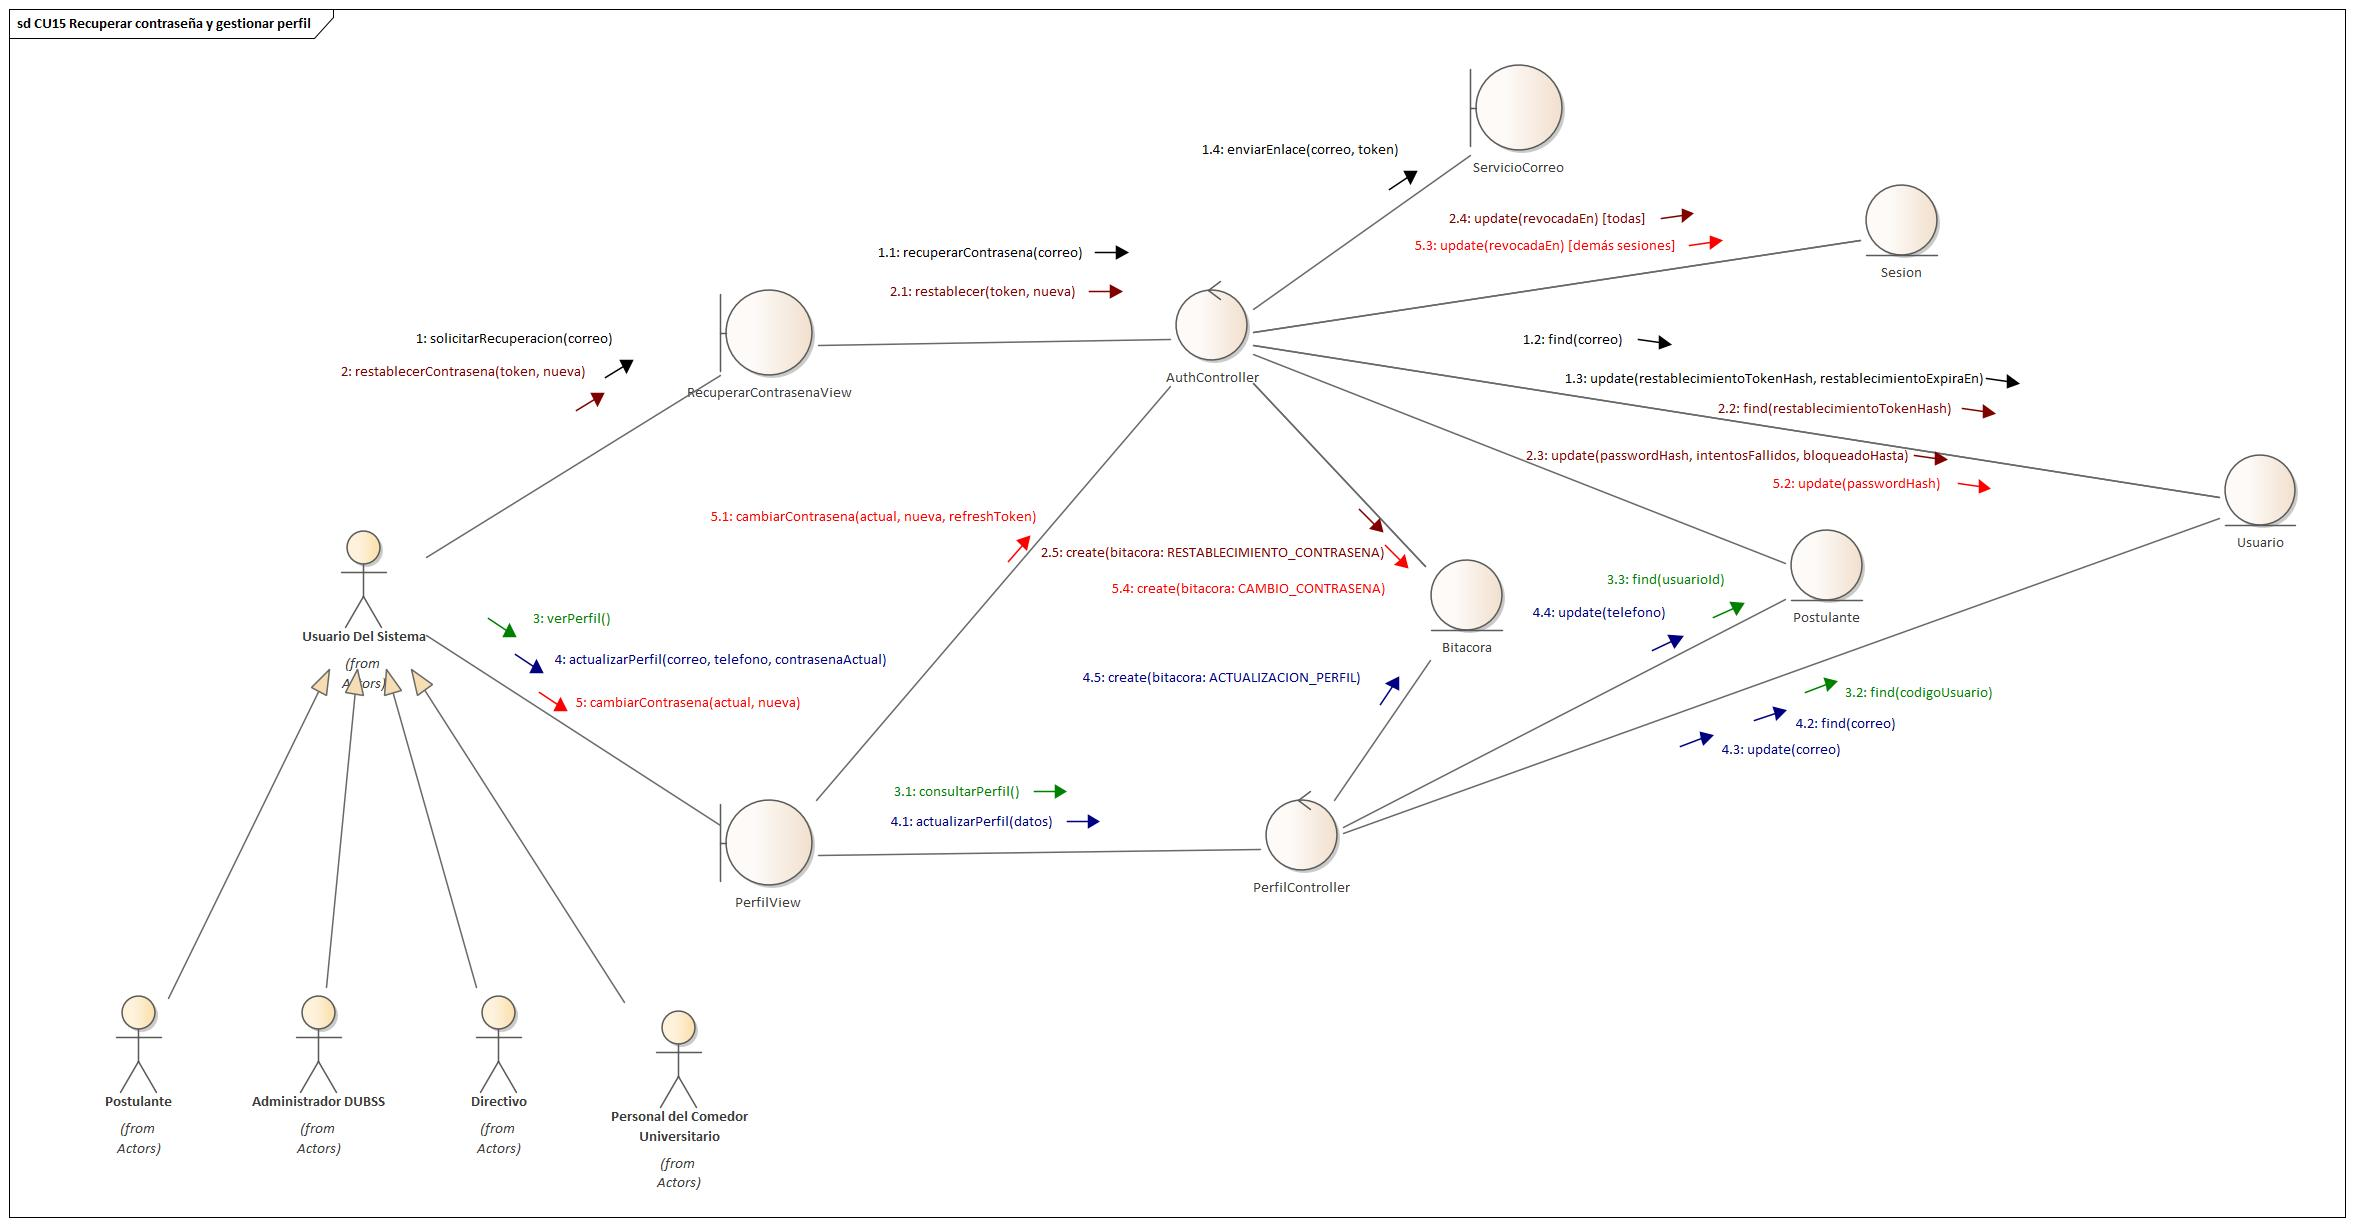
\includegraphics[width=\textwidth,height=0.5\textheight,keepaspectratio]{images/057_Analisis_CU15_Recuperar_Contrasena_Gestionar_Perfil.png}

\smallskip
\noindent\raggedright\textit{Nota.} Elaboración propia.
\end{figure}

La solicitud de recuperación (mensaje 1) consulta al usuario por su correo (1.2), guarda en él el hash del token de un solo uso y su vencimiento (1.3) y envía el enlace por correo (1.4); la respuesta es siempre el mismo mensaje neutro. El restablecimiento (mensaje 2) busca la cuenta por el hash del token (2.2), guarda la nueva contraseña y desbloquea la cuenta (2.3), revoca todas sus sesiones (2.4) y lo registra en la bitácora (2.5). La consulta del perfil (mensaje 3) obtiene los datos del usuario (3.2) y, si es Postulante, los suyos (3.3). La actualización (mensaje 4) verifica que el correo nuevo no pertenezca a otra cuenta (4.2), actualiza el correo (4.3) y el teléfono del postulante (4.4) y lo registra en la bitácora (4.5). El cambio de contraseña (mensaje 5) actualiza la contraseña (5.2), revoca las sesiones de los demás dispositivos (5.3) y lo registra en la bitácora (5.4).


\subsubsection{6.2.16. Analizar CU-16 Digitalizar y adjuntar documentos}\label{sec:cap6_analisis_cu16}

En el CU-16, el Postulante adjunta los documentos de respaldo mediante \textit{DocumentoView} y \textit{DocumentoController}, que utilizan las entidades \textit{ConvocatoriaDocumento} y \textit{DocumentoAdjunto}. La Figura~\ref{fig:analisis_cu16} presenta el diagrama de análisis.

\begin{figure}[H]
\caption{Análisis del CU-16 Digitalizar y adjuntar documentos}
\label{fig:analisis_cu16}
\centering
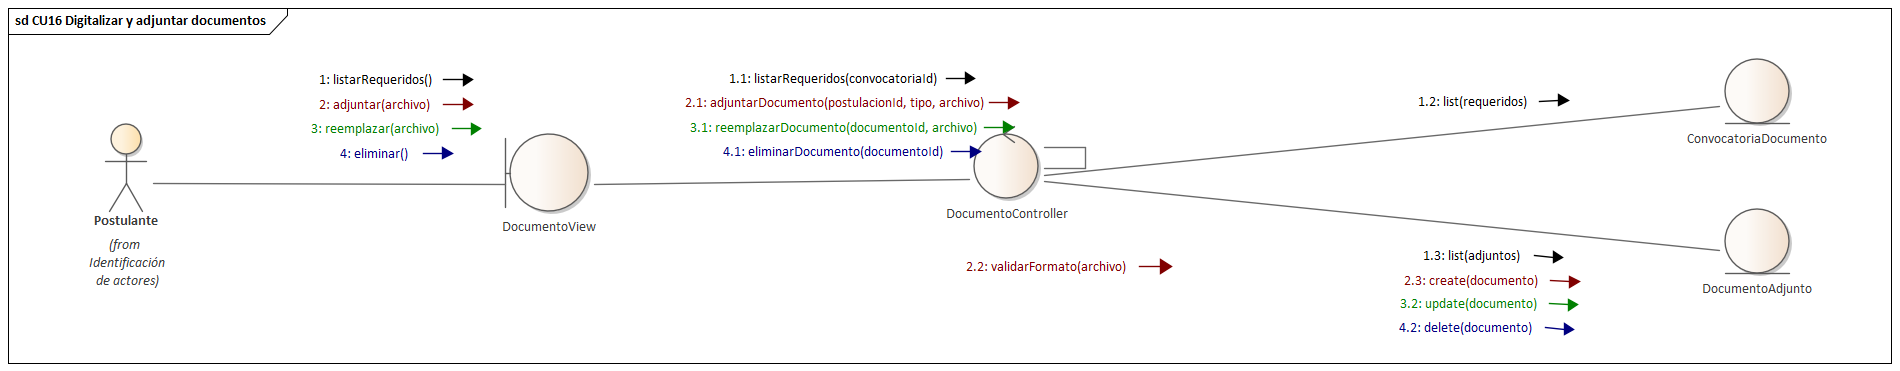
\includegraphics[width=\textwidth,height=0.5\textheight,keepaspectratio]{images/058_Analisis_CU16_Digitalizar_Adjuntar_Documentos.png}

\smallskip
\noindent\raggedright\textit{Nota.} Elaboración propia.
\end{figure}

Primero se listan los documentos requeridos por la convocatoria y los ya adjuntados (mensaje 1, con los pasos 1.2 y 1.3). Al adjuntar un archivo (mensaje 2), el controlador valida su formato (2.2) y crea el documento adjunto (2.3). El reemplazo (mensaje 3) actualiza el documento (3.2) y la eliminación (mensaje 4) lo elimina (4.2), operaciones permitidas antes del envío de la postulación o cuando esta fue devuelta.


\subsubsection{6.2.17. Analizar CU-17 Guardar borrador de postulación}\label{sec:cap6_analisis_cu17}

En el CU-17, el Postulante guarda y retoma su postulación incompleta mediante \textit{BorradorView} y \textit{BorradorController}, que trabajan con las entidades \textit{Convocatoria}, \textit{Postulacion} y \textit{RespuestaSocioeconomica}. La Figura~\ref{fig:analisis_cu17} presenta el diagrama de análisis.

\begin{figure}[H]
\caption{Análisis del CU-17 Guardar borrador de postulación}
\label{fig:analisis_cu17}
\centering
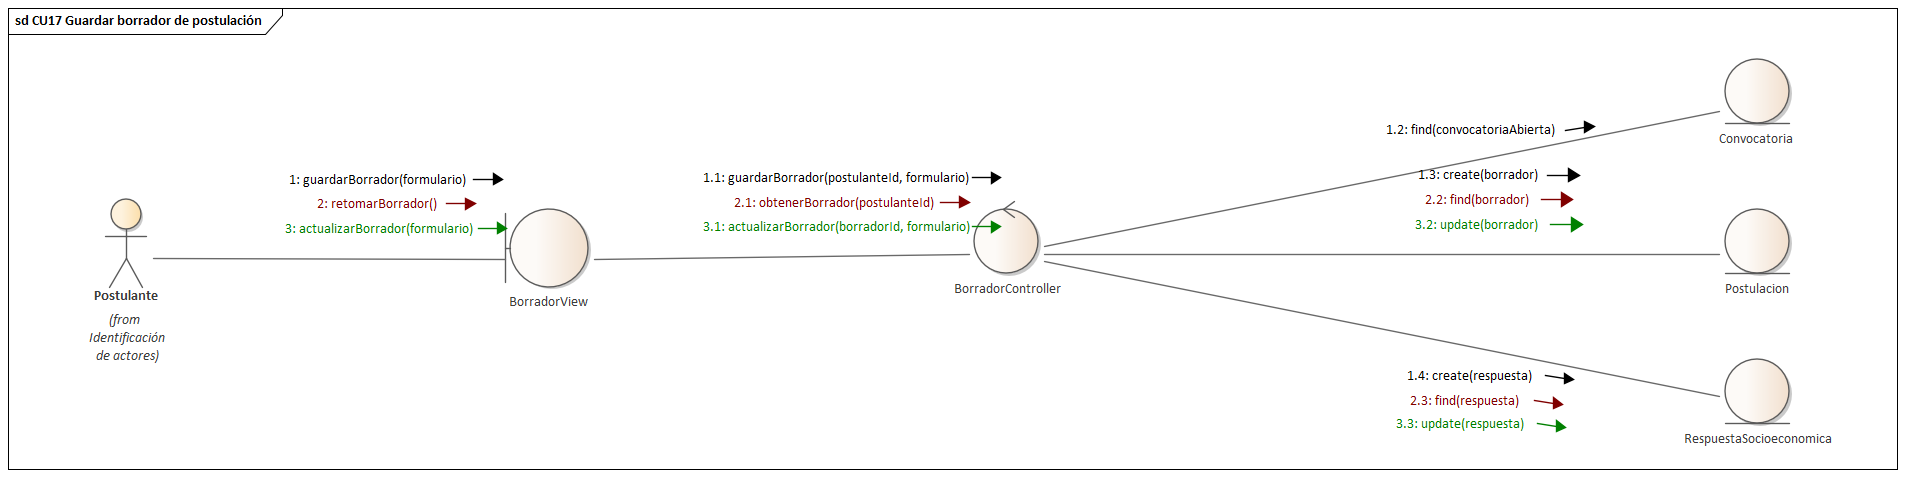
\includegraphics[width=\textwidth,height=0.5\textheight,keepaspectratio]{images/059_Analisis_CU17_Guardar_Borrador_Postulacion.png}

\smallskip
\noindent\raggedright\textit{Nota.} Elaboración propia.
\end{figure}

Al guardar el borrador (mensaje 1), el controlador verifica que la convocatoria esté abierta (1.2) y crea la postulación en estado de borrador (1.3) con las respuestas ingresadas (1.4), sin exigir los campos obligatorios. Al retomarlo (mensaje 2) se recuperan el borrador (2.2) y sus respuestas (2.3), y al continuar editándolo (mensaje 3) se actualizan ambos (3.2 y 3.3). El borrador no se envía al módulo de precalificación.


\subsubsection{6.2.18. Analizar CU-18 Validar elegibilidad y duplicados}\label{sec:cap6_analisis_cu18}

El CU-18 es incluido por el CU-02: se ejecuta cuando el Postulante envía su postulación a través de \textit{PostulacionView}. El controlador \textit{ValidacionController} colabora con las entidades \textit{Postulante}, \textit{Convocatoria} y \textit{Postulacion}. La Figura~\ref{fig:analisis_cu18} presenta el diagrama de análisis.

\begin{figure}[H]
\caption{Análisis del CU-18 Validar elegibilidad y duplicados}
\label{fig:analisis_cu18}
\centering
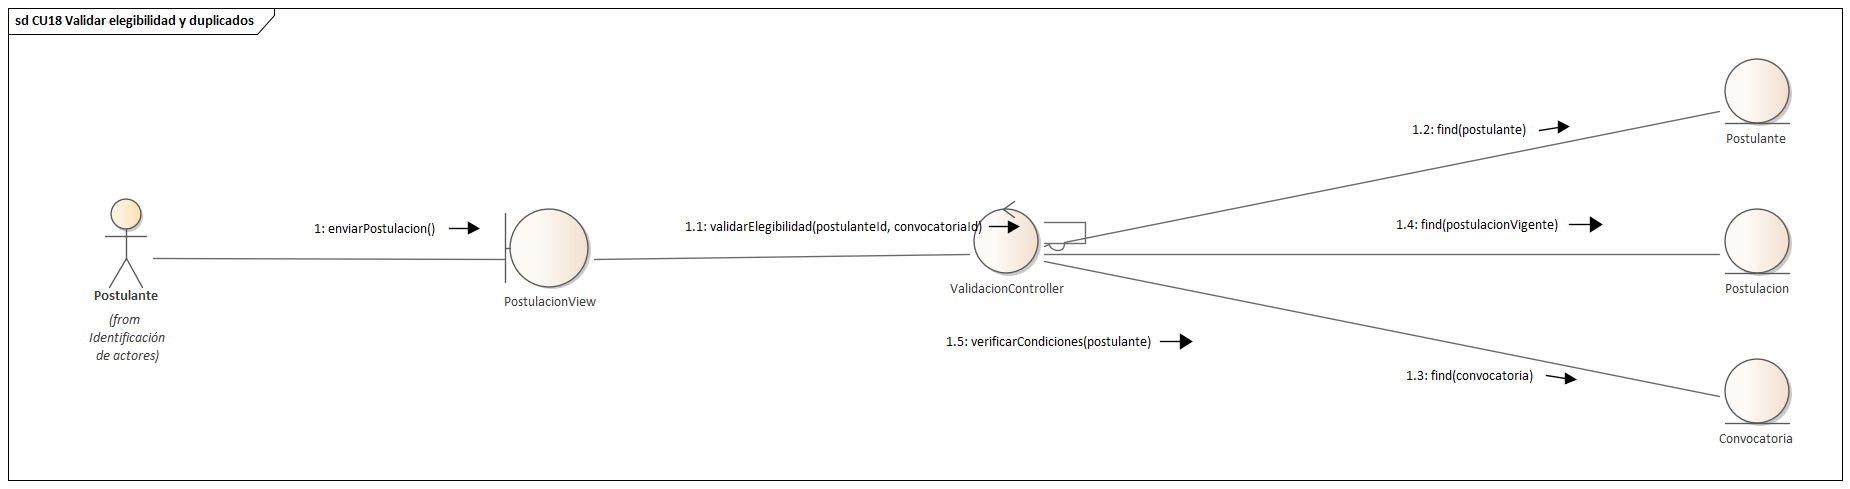
\includegraphics[width=\textwidth,height=0.5\textheight,keepaspectratio]{images/060_Analisis_CU18_Validar_Elegibilidad_Duplicados.png}

\smallskip
\noindent\raggedright\textit{Nota.} Elaboración propia.
\end{figure}

Con la solicitud de validación (mensaje 1.1), el controlador consulta al postulante (1.2), la convocatoria (1.3) y la postulación vigente del postulante en la misma gestión (1.4), y verifica las condiciones de elegibilidad (1.5). El resultado determina si el CU-02 puede registrar la postulación o debe rechazarla indicando el motivo.


\subsubsection{6.2.19. Analizar CU-19 Devolver postulación para corrección}\label{sec:cap6_analisis_cu19}

En el CU-19, el Administrador DUBSS devuelve una postulación mediante \textit{DevolverPostulacionView} y \textit{DevolucionController}, que utiliza las entidades \textit{Finalista}, \textit{Postulacion}, \textit{PostulacionHistorial}, \textit{Bitacora} y \textit{Notificacion}. La Figura~\ref{fig:analisis_cu19} presenta el diagrama de análisis.

\begin{figure}[H]
\caption{Análisis del CU-19 Devolver postulación para corrección}
\label{fig:analisis_cu19}
\centering
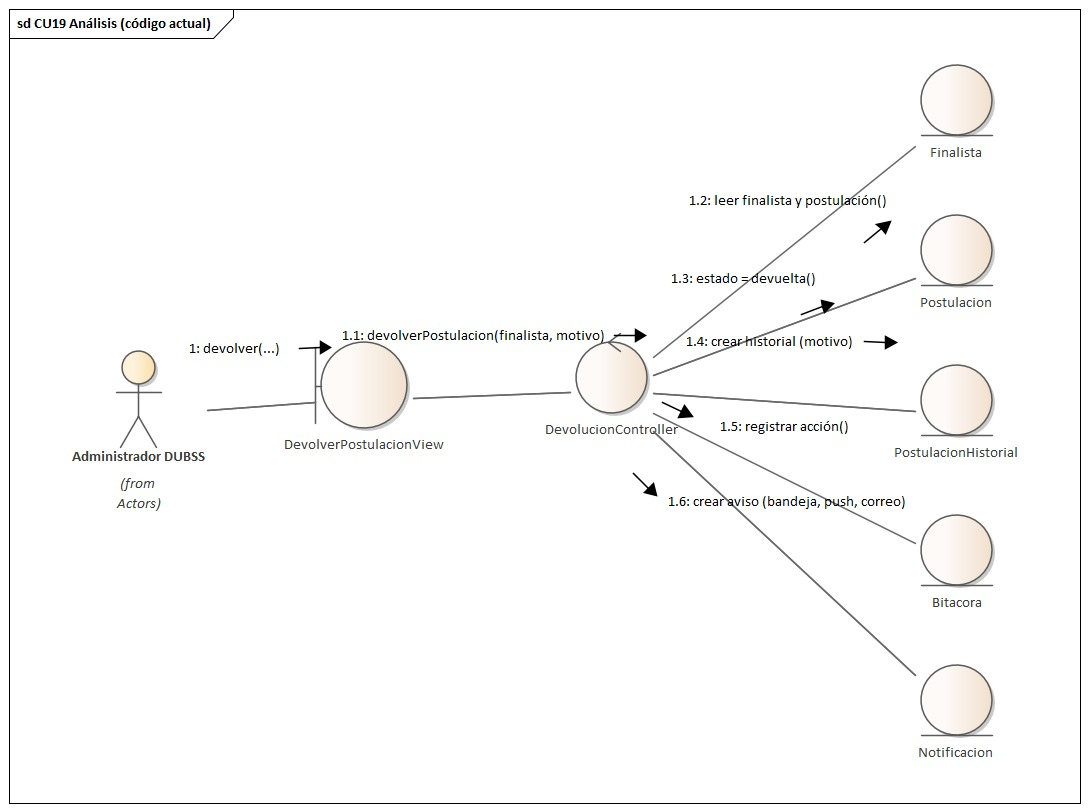
\includegraphics[width=\textwidth,height=0.5\textheight,keepaspectratio]{images/085_Analisis_CU19_Devolver_Postulacion_Correccion.jpg}

\smallskip
\noindent\raggedright\textit{Nota.} Elaboración propia.
\end{figure}

Al devolver la postulación con su motivo (mensaje 1), el controlador entra por el código del finalista, lee el finalista y su postulación y valida que siga «calificada»; a continuación actualiza su estado a «devuelta», crea el registro del cambio en el historial de la postulación con el motivo (hasta 500 caracteres), registra la acción en la bitácora y crea la notificación dirigida al Postulante, que se envía por bandeja, push y correo.


\subsubsection{6.2.20. Analizar CU-20 Archivar o rechazar postulación}\label{sec:cap6_analisis_cu20}

En el CU-20, el Administrador DUBSS cierra una postulación mediante \textit{ArchivarPostulacionView} y \textit{ArchivoController}, que trabajan con las entidades \textit{Postulacion} y \textit{PostulacionHistorial}. La Figura~\ref{fig:analisis_cu20} presenta el diagrama de análisis.

\begin{figure}[H]
\caption{Análisis del CU-20 Archivar o rechazar postulación}
\label{fig:analisis_cu20}
\centering
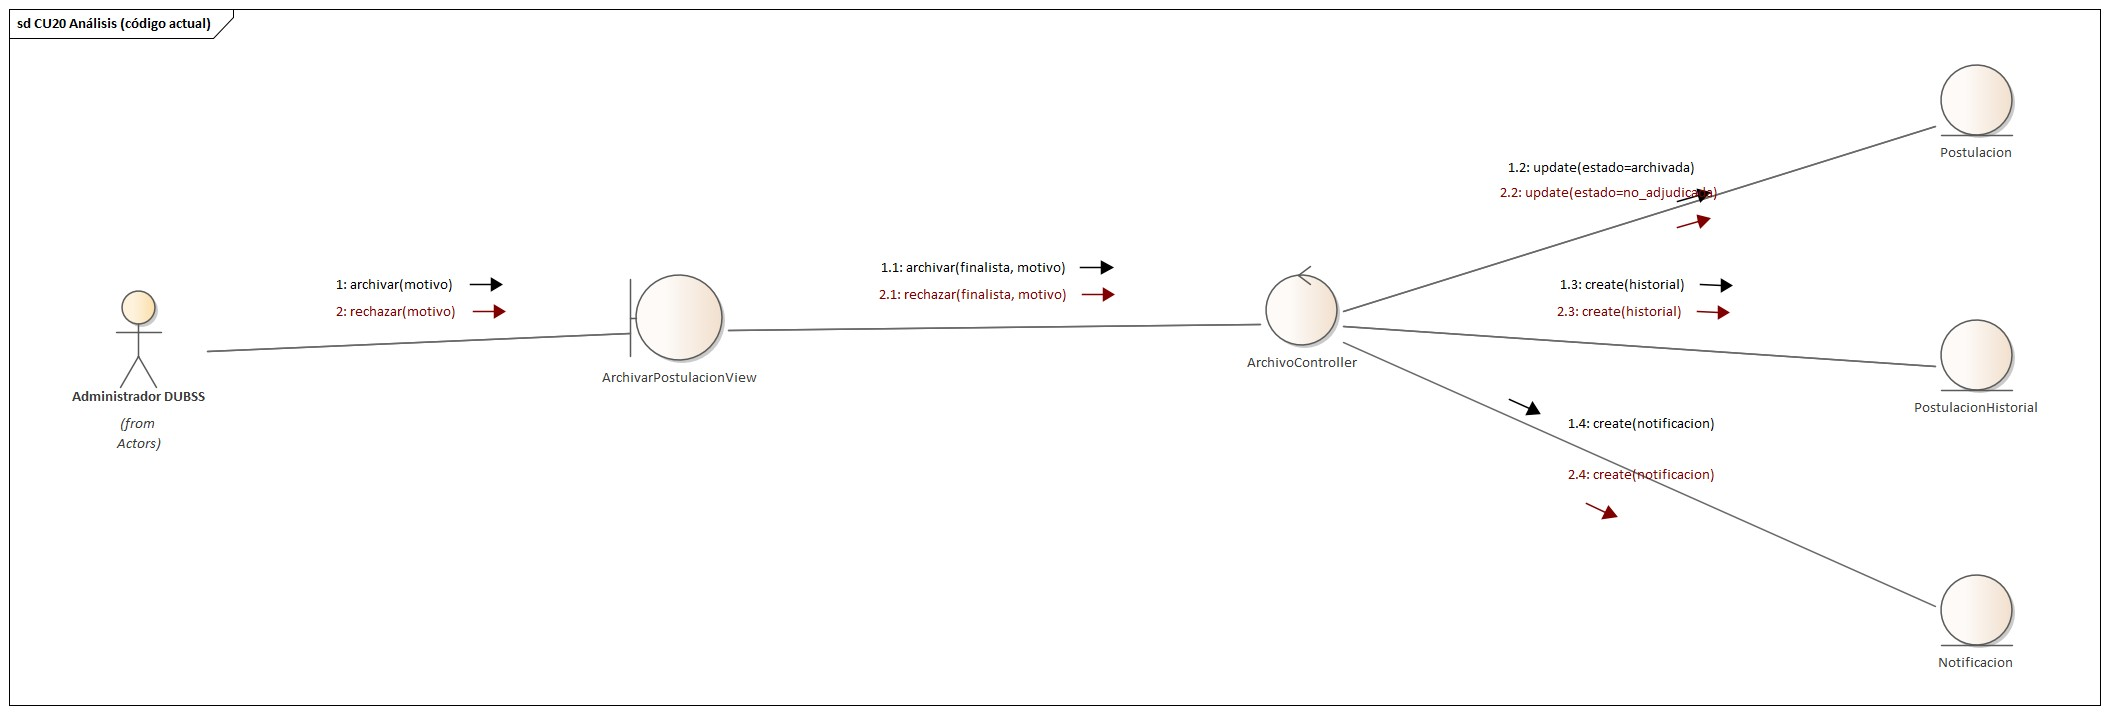
\includegraphics[width=\textwidth,height=0.5\textheight,keepaspectratio]{images/086_Analisis_CU20_Archivar_Rechazar_Postulacion.jpg}

\smallskip
\noindent\raggedright\textit{Nota.} Elaboración propia.
\end{figure}

Al archivar la postulación (mensaje 1), el controlador actualiza su estado a «archivada» (1.2) y registra el cambio con su motivo en el historial (1.3). Al rechazarla (mensaje 2), el controlador actualiza su estado a «no adjudicada» (2.2) y registra igualmente el cambio en el historial (2.3).


\subsubsection{6.2.21. Analizar CU-21 Notificar finalistas, registrar entrega de documentación física y publicar comunicados/avisos}\label{sec:cap6_analisis_cu21}

En el CU-21 participan dos actores: el Administrador DUBSS, que gestiona a los finalistas mediante \textit{FinalistaView}, y el Postulante, que recibe los avisos mediante \textit{AvisoView}. Ambas interfaces se comunican con un único controlador, \textit{NotificacionController}, que utiliza las entidades \textit{Finalista}, \textit{Notificacion} y \textit{Comunicado}. El envío de la notificación push se modela como un mensaje del propio controlador (2.4 y 4.4). La Figura~\ref{fig:analisis_cu21} presenta el diagrama de análisis.

\begin{figure}[H]
\caption{Análisis del CU-21 Notificar finalistas, registrar entrega de documentación física y publicar comunicados/avisos}
\label{fig:analisis_cu21}
\centering
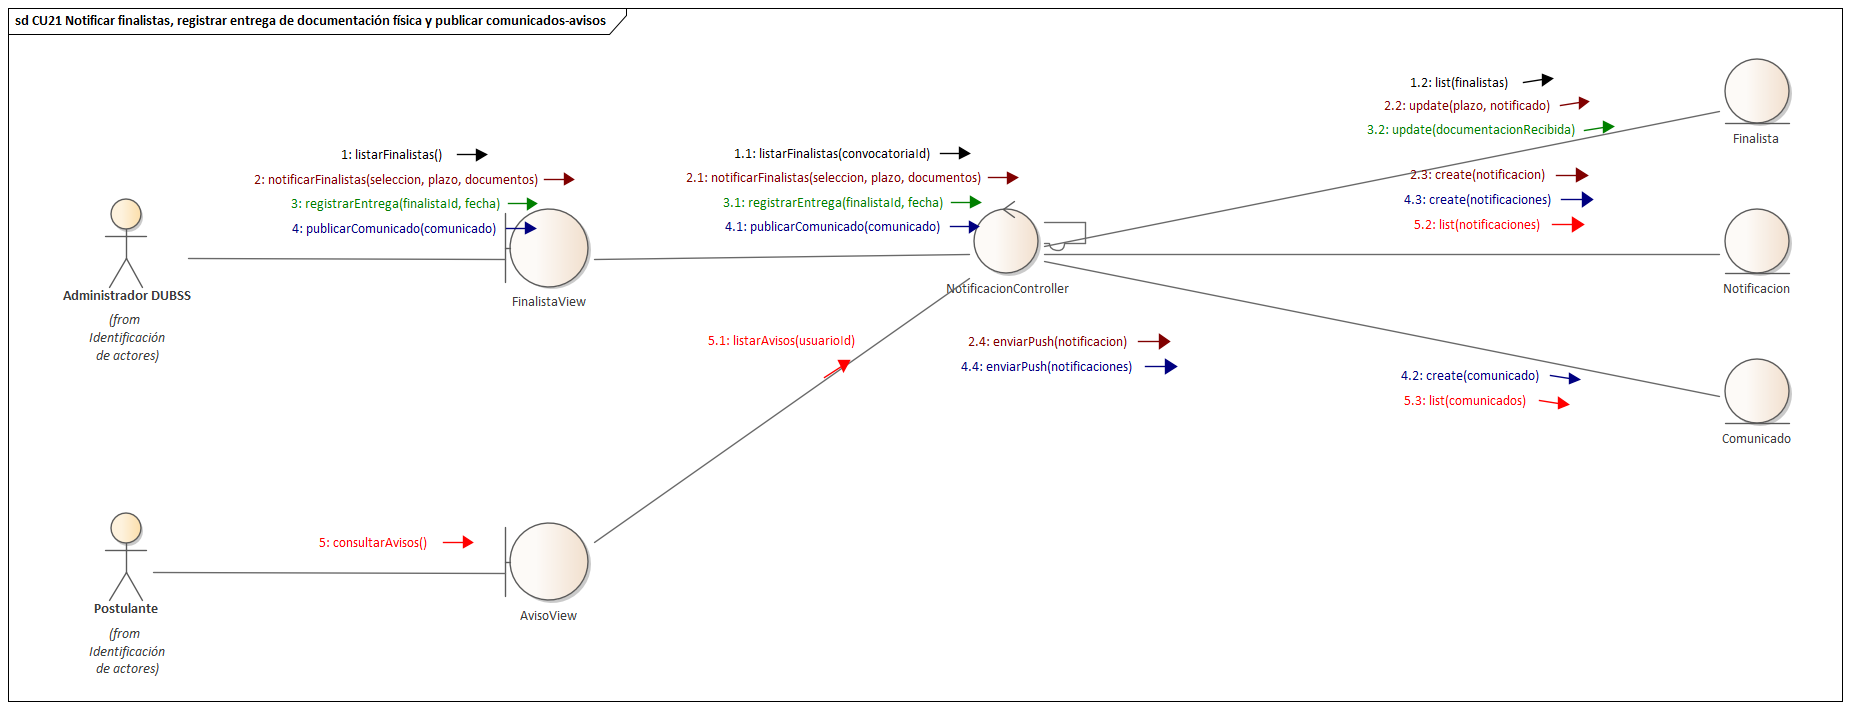
\includegraphics[width=\textwidth,height=0.5\textheight,keepaspectratio]{images/061_Analisis_CU21_Notificar_Finalistas_Publicar_Avisos.png}

\smallskip
\noindent\raggedright\textit{Nota.} Elaboración propia.
\end{figure}

El Administrador puede listar los finalistas (mensaje 1), notificarlos con el plazo y los documentos que deben presentar (mensaje 2), lo que actualiza al finalista (2.2) y crea la notificación (2.3); registrar la entrega de la documentación física (mensaje 3), que actualiza al finalista (3.2); y publicar un comunicado (mensaje 4), que crea el comunicado (4.2) y las notificaciones correspondientes (4.3). El Postulante consulta sus avisos (mensaje 5), con lo que se listan sus notificaciones (5.2) y los comunicados (5.3).


\subsubsection{6.2.22. Analizar CU-22 Publicar resultados de adjudicación}\label{sec:cap6_analisis_cu22}

En el CU-22, el Administrador DUBSS publica los resultados mediante \textit{PublicarResultadosView} y \textit{ResultadosController}, que colaboran con las entidades \textit{Adjudicacion}, \textit{PublicacionResultado} y \textit{Notificacion}. El envío de las notificaciones push se modela como un mensaje del propio controlador (2.4). La Figura~\ref{fig:analisis_cu22} presenta el diagrama de análisis.

\begin{figure}[H]
\caption{Análisis del CU-22 Publicar resultados de adjudicación}
\label{fig:analisis_cu22}
\centering
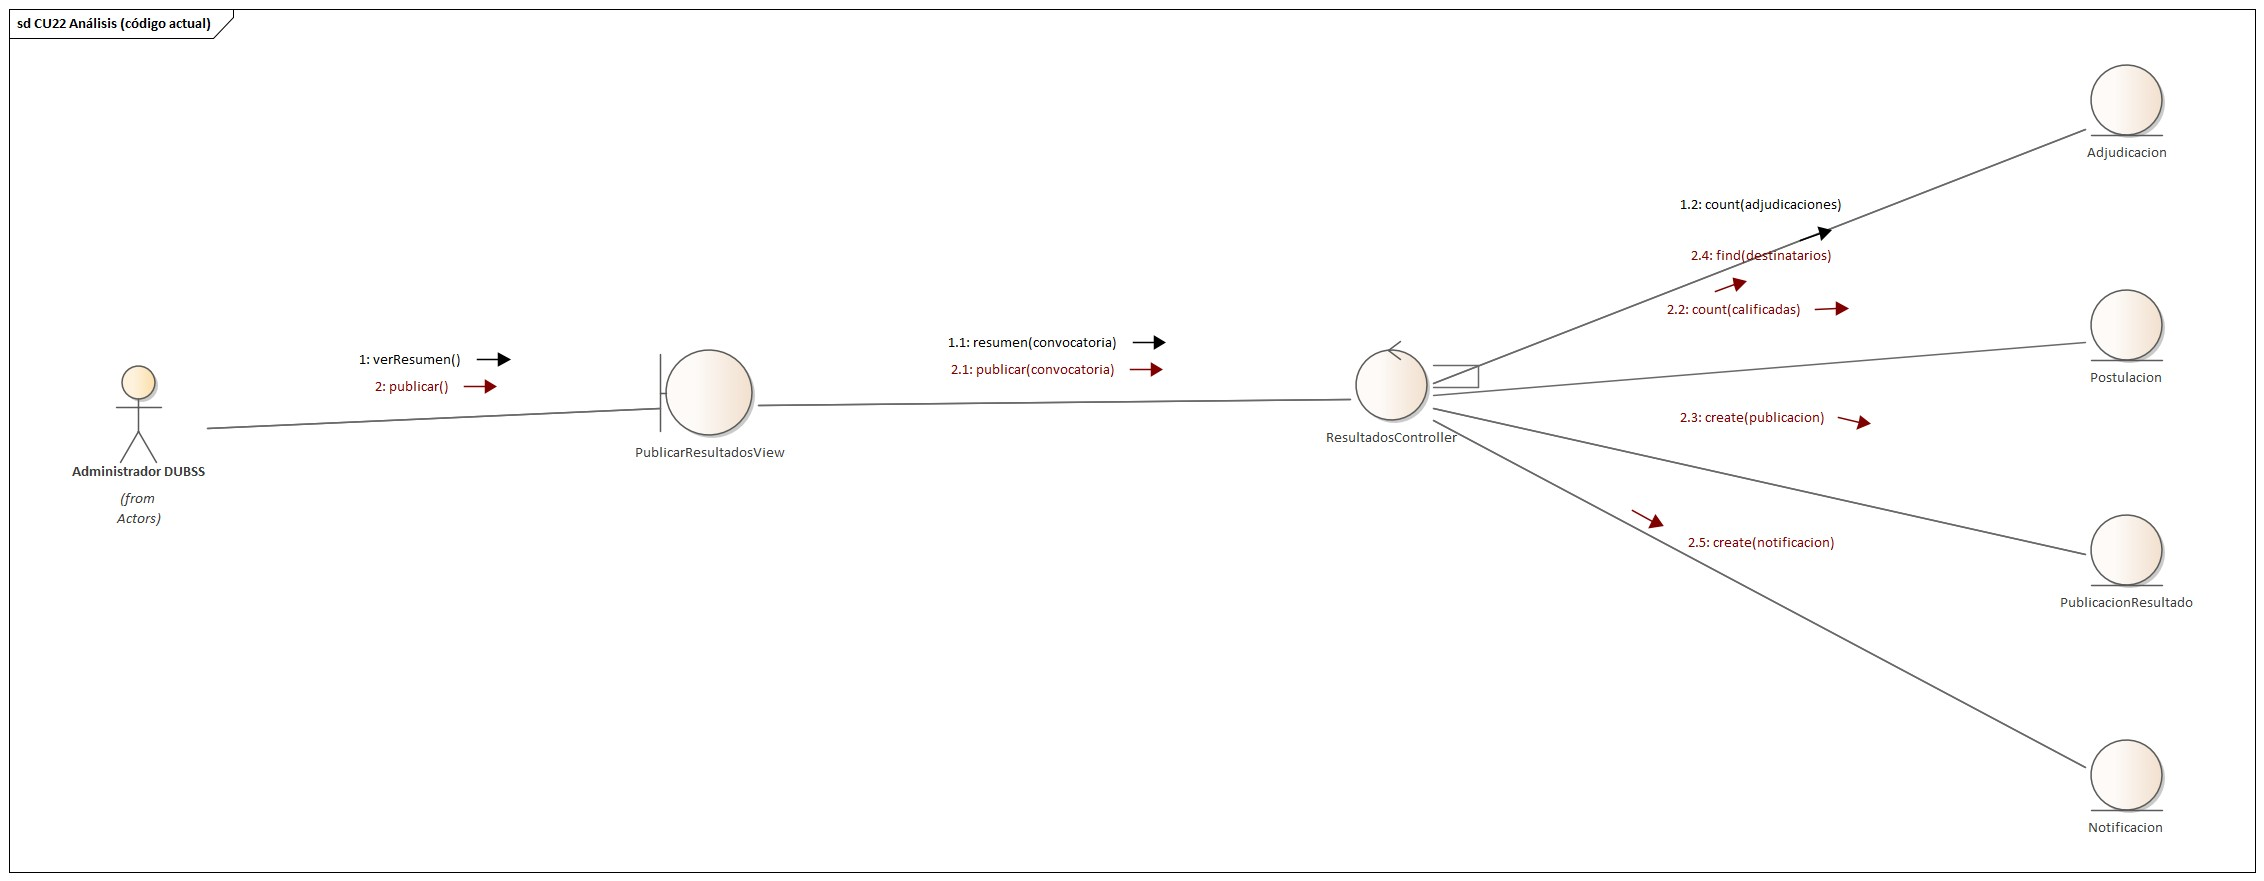
\includegraphics[width=\textwidth,height=0.5\textheight,keepaspectratio]{images/087_Analisis_CU22_Publicar_Resultados_Adjudicacion.jpg}

\smallskip
\noindent\raggedright\textit{Nota.} Elaboración propia.
\end{figure}

Al ver los resultados (mensaje 1), el controlador lista las adjudicaciones de la convocatoria (1.2). Al publicarlos (mensaje 2), el controlador crea el registro de la publicación (2.2), crea las notificaciones dirigidas a los postulantes (2.3) y las envía como notificaciones push (2.4).


\subsubsection{6.2.23. Analizar CU-23 Gestionar padrón de becados (baja, suspensión, reemplazo)}\label{sec:cap6_analisis_cu23}

En el CU-23, el Administrador DUBSS gestiona el padrón mediante \textit{PadronView} y \textit{PadronController}, que utilizan las entidades \textit{Beca} y \textit{MovimientoBeca}. La Figura~\ref{fig:analisis_cu23} presenta el diagrama de análisis.

\begin{figure}[H]
\caption{Análisis del CU-23 Gestionar padrón de becados (baja, suspensión, reemplazo)}
\label{fig:analisis_cu23}
\centering
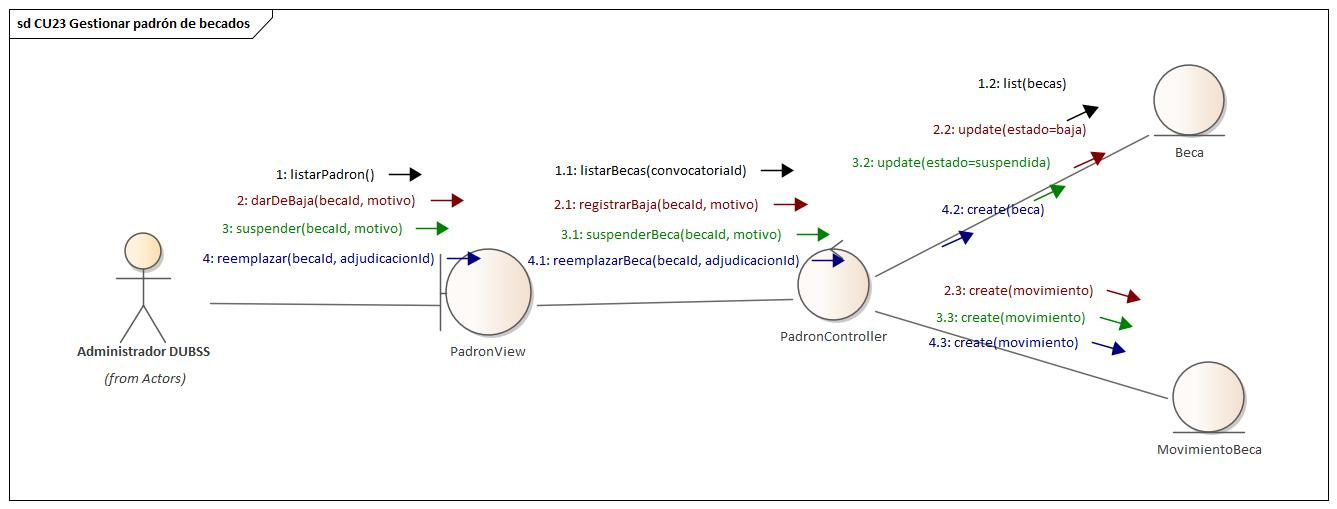
\includegraphics[width=\textwidth,height=0.5\textheight,keepaspectratio]{images/088_Analisis_CU23_Gestionar_Padron_Becados.jpg}

\smallskip
\noindent\raggedright\textit{Nota.} Elaboración propia.
\end{figure}

Al listar el padrón (mensaje 1), el controlador obtiene las becas de la convocatoria (1.2). Al dar de baja una beca (mensaje 2), actualiza su estado a «baja» (2.2) y crea el movimiento correspondiente (2.3). Al suspenderla (mensaje 3), actualiza su estado a «suspendida» (3.2) y crea el movimiento (3.3). Al reemplazar un cupo liberado (mensaje 4), crea una nueva beca para el postulante reemplazante (4.2) y registra el movimiento de reemplazo (4.3).


\subsubsection{6.2.24. Analizar CU-24 Consultar historial de asistencia y estado de beca}\label{sec:cap6_analisis_cu24}

En el CU-24, el Postulante adjudicado (becado) consulta su beca mediante \textit{MiBecaView}, que se apoya en \textit{MiBecaController}. Las entidades involucradas son \textit{Beca}, \textit{MovimientoBeca} y \textit{Asistencia}. La Figura~\ref{fig:analisis_cu24} presenta el diagrama de análisis.

\begin{figure}[H]
\caption{Análisis del CU-24 Consultar historial de asistencia y estado de beca}
\label{fig:analisis_cu24}
\centering
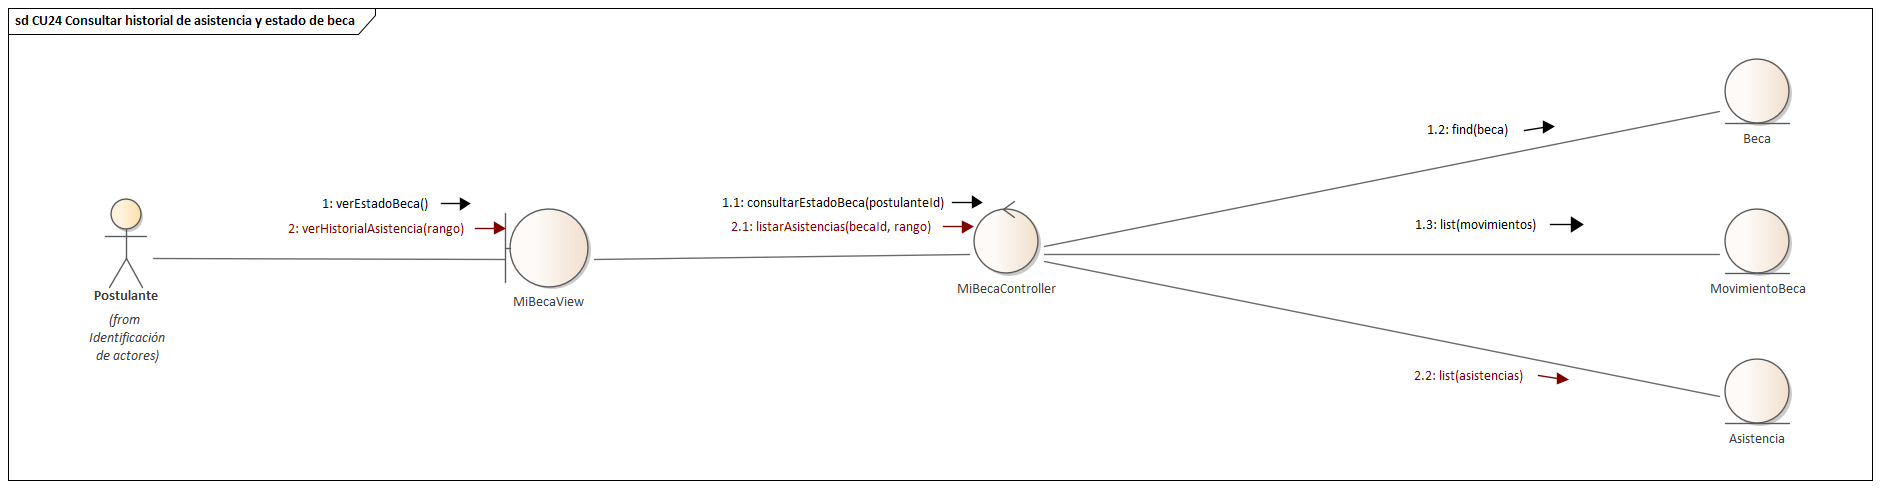
\includegraphics[width=\textwidth,height=0.5\textheight,keepaspectratio]{images/062_Analisis_CU24_Consultar_Historial_Asistencia_Beca.png}

\smallskip
\noindent\raggedright\textit{Nota.} Elaboración propia.
\end{figure}

Para ver el estado de su beca (mensaje 1), el controlador obtiene la beca del postulante (1.2) y sus movimientos de baja, suspensión o reemplazo (1.3). Para ver el historial de asistencia (mensaje 2), lista las asistencias de la beca dentro del rango indicado (2.2). Ambas operaciones son de solo lectura y el becado accede únicamente a su propia información.


\subsubsection{6.2.25. Analizar CU-25 Consultar bitácora de acciones}\label{sec:cap6_analisis_cu25}

En el CU-25, el Administrador DUBSS consulta la bitácora mediante \textit{BitacoraView} y \textit{BitacoraController}. La única entidad involucrada es \textit{Bitacora}, que almacena los registros de las acciones relevantes del sistema. La Figura~\ref{fig:analisis_cu25} presenta el diagrama de análisis.

\begin{figure}[H]
\caption{Análisis del CU-25 Consultar bitácora de acciones}
\label{fig:analisis_cu25}
\centering
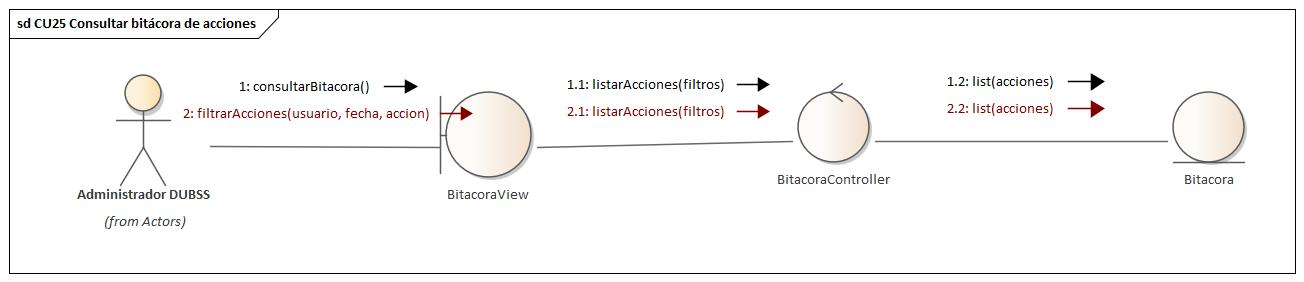
\includegraphics[width=\textwidth,height=0.5\textheight,keepaspectratio]{images/089_Analisis_CU25_Consultar_Bitacora_Acciones.jpg}

\smallskip
\noindent\raggedright\textit{Nota.} Elaboración propia.
\end{figure}

Al consultar la bitácora (mensaje 1), el controlador lista las acciones registradas (1.2). Al filtrar las acciones por usuario, fecha y tipo de acción (mensaje 2), el controlador repite la consulta con los filtros indicados (2.2). Ambas operaciones son de solo lectura y no permiten modificar los registros.


\subsubsection{6.2.26. Analizar CU-26 Parametrizar modelo de preselección y reprocesar puntajes}\label{sec:cap6_analisis_cu26}

En el CU-26, el Administrador DUBSS ajusta el modelo de preselección mediante \textit{ModeloPreseleccionView} y \textit{ModeloPreseleccionController}, que colaboran con las entidades \textit{ModeloPreseleccion}, \textit{ParametroModelo}, \textit{LoteReprocesamiento} y \textit{PuntajePostulacion}. El recálculo de puntajes se modela como el mensaje 3.3 del propio controlador. La Figura~\ref{fig:analisis_cu26} presenta el diagrama de análisis.

\begin{figure}[H]
\caption{Análisis del CU-26 Parametrizar modelo de preselección y reprocesar puntajes}
\label{fig:analisis_cu26}
\centering
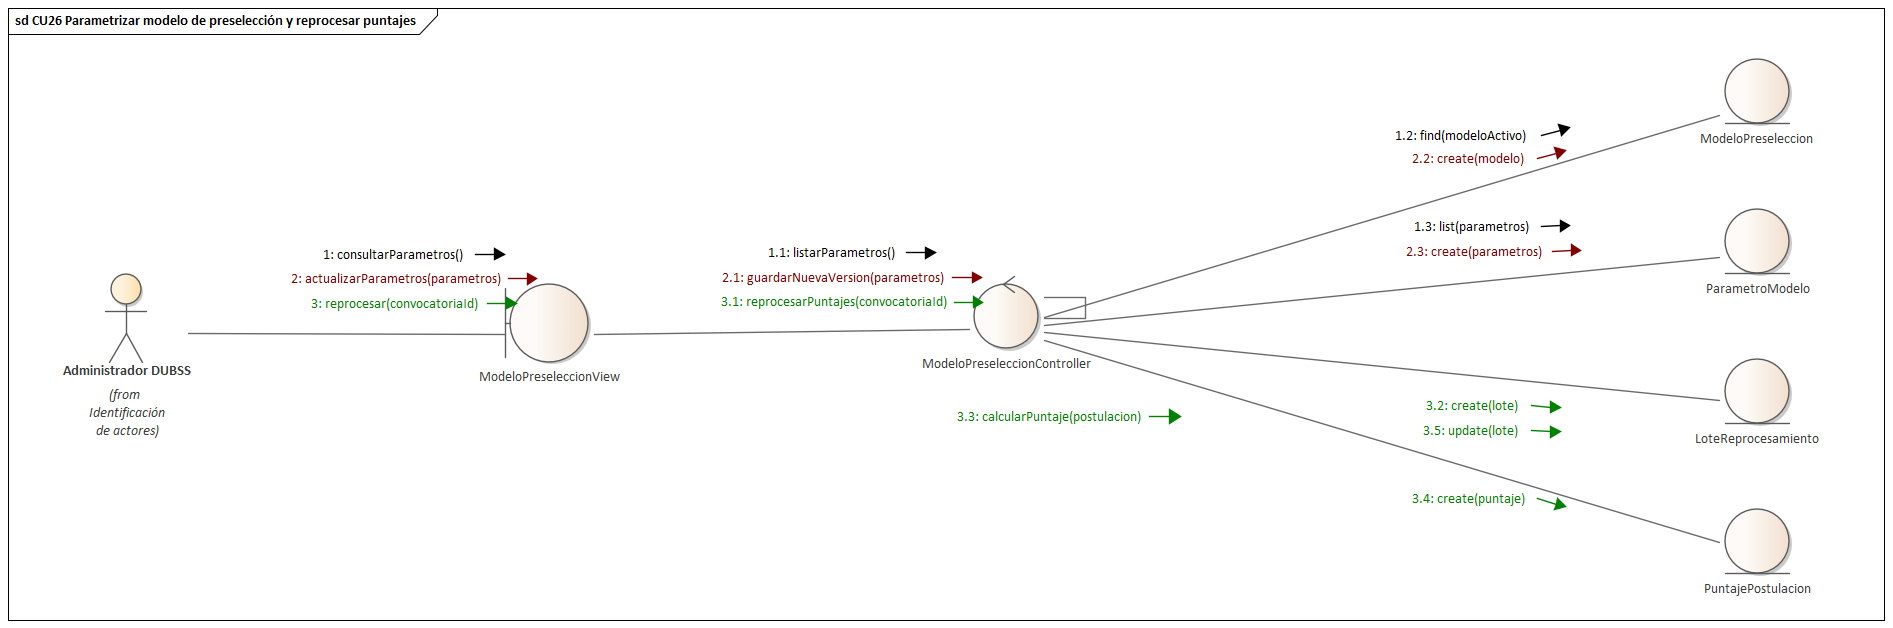
\includegraphics[width=\textwidth,height=0.5\textheight,keepaspectratio]{images/063_Analisis_CU26_Parametrizar_Modelo_Preseleccion.png}

\smallskip
\noindent\raggedright\textit{Nota.} Elaboración propia.
\end{figure}

La consulta de parámetros (mensaje 1) obtiene el modelo activo (1.2) y sus parámetros (1.3). Al actualizarlos (mensaje 2), se crea una nueva versión del modelo (2.2) con sus parámetros (2.3), conservando las versiones anteriores. El reprocesamiento (mensaje 3) crea un lote (3.2), recalcula el puntaje de las postulaciones (3.3), registra los nuevos puntajes (3.4), conservando los anteriores, y actualiza el estado del lote (3.5).


% ------------------------------------------------------------------------------
% 6.3. ANÁLISIS DE PAQUETES
% ------------------------------------------------------------------------------
\wfa{\wn{6}.3. Análisis de Paquetes}\label{sec:cap6_analisis_paquetes}

% [PENDIENTE]: Realizar el análisis de cada paquete identificado.

La Figura~\ref{fig:analisis_paquetes} presenta el diagrama de análisis de paquetes del sistema y las dependencias entre los seis paquetes identificados.

\begin{figure}[H]
\caption{Diagrama de análisis de paquetes del Sistema Web y Móvil de Postulación y Preselección de la Beca Comedor}
\label{fig:analisis_paquetes}
\centering
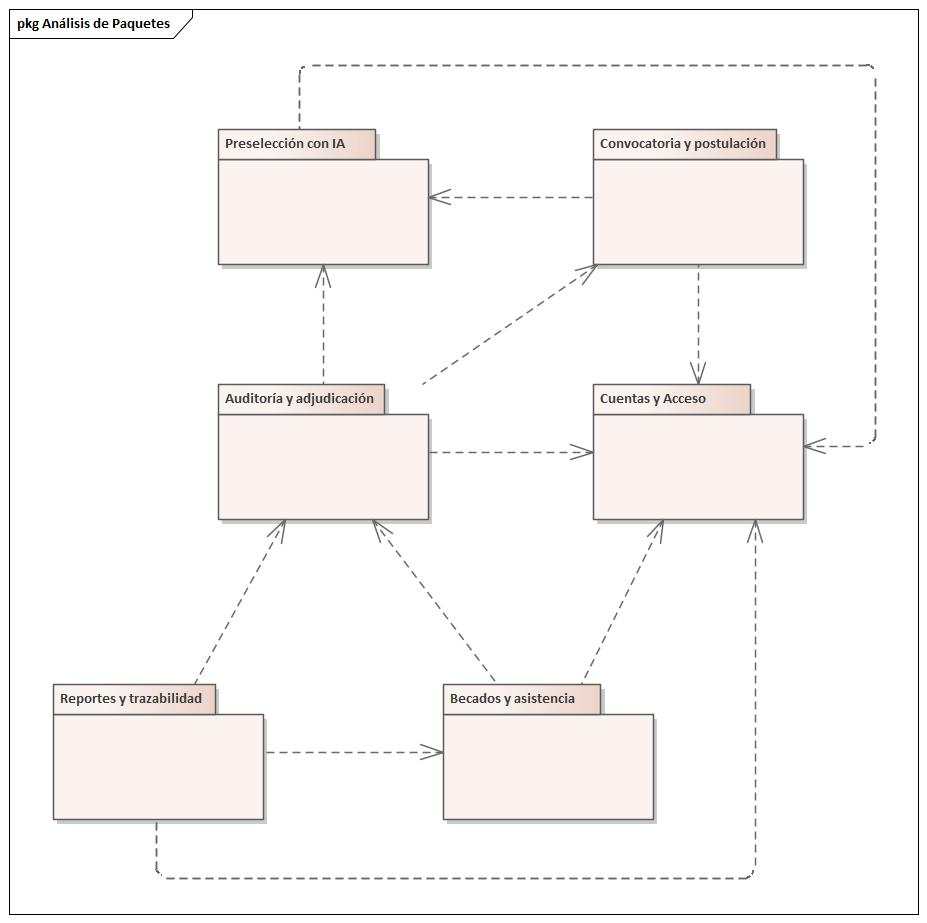
\includegraphics[width=\textwidth,height=0.85\textheight,keepaspectratio]{images/028_Analisis_Paquetes.jpg}

\smallskip
\noindent\raggedright\textit{Nota.} Elaboración propia.
\end{figure}



% ==============================================================================
% 3.4 DISEÑO (flujo de trabajo PUDS)
% Reutiliza el cap. 7 de main.tex.
% ==============================================================================
\subsection{3.4. Diseño}\label{sec:v2_diseno}

Este flujo de trabajo del PUDS define la arquitectura física y lógica, el diagrama de clases, el diseño de datos (lógico y físico), el diseño de cada caso de uso y el diseño de las interfaces.

% ------------------------------------------------------------------------------
% 7.1. DISEÑO DE LA ARQUITECTURA
% ------------------------------------------------------------------------------
\subsection{7.1. Diseño de la Arquitectura}\label{sec:cap7_arquitectura}

% [PENDIENTE]: Redactar la introducción del diseño de la arquitectura.

\subsubsection{7.1.1. Diseño Físico}\label{sec:cap7_diseno_fisico}

El diseño físico describe la arquitectura física del sistema, es decir, su topología: los nodos de hardware y los entornos de ejecución, junto con los artefactos de software que se ejecutan en cada uno y los protocolos de comunicación entre ellos. Se representa mediante un diagrama de despliegue del Lenguaje Unificado de Modelado \parencite{booch2005uml, rumbaugh2004uml}.

El sistema se organiza en tres grupos de nodos. El primero corresponde al cliente: la aplicación web (React y TypeScript), que se ejecuta en el navegador de una computadora personal, y la aplicación móvil (Flutter), que se ejecuta en un dispositivo Android y utiliza la cámara para digitalizar los documentos de la postulación. El segundo grupo corresponde a la nube de Amazon Web Services (AWS), que contiene un servidor de aplicación con Docker Engine, donde se ejecutan en contenedores separados la API REST (Java y Spring Boot, que emite y verifica los tokens JWT de autenticación) y el servicio de preselección en Python; un servidor de base de datos con PostgreSQL; y MinIO (almacenamiento de objetos compatible con S3) para el almacenamiento de los documentos adjuntos, las actas de adjudicación y las planillas de asistencia en formato PDF. El tercer grupo reúne los servicios externos de Firebase, de los cuales se emplea Firebase Cloud Messaging (FCM) para el envío de notificaciones \textit{push} al dispositivo móvil.

Las aplicaciones cliente se comunican con la API REST mediante HTTPS en formato JSON; el módulo de preselección solo es accesible desde la API, mediante una interfaz interna HTTP, y no se expone a los clientes. La API accede a PostgreSQL mediante JDBC, a MinIO mediante su API compatible con S3 y a FCM mediante el SDK de administración de Firebase. La Figura~\ref{fig:diagrama_despliegue} presenta el diagrama de despliegue general del sistema.

\begin{landscape}
\begin{figure}[p]
\caption{Diagrama de despliegue general del sistema}
\label{fig:diagrama_despliegue}
\centering
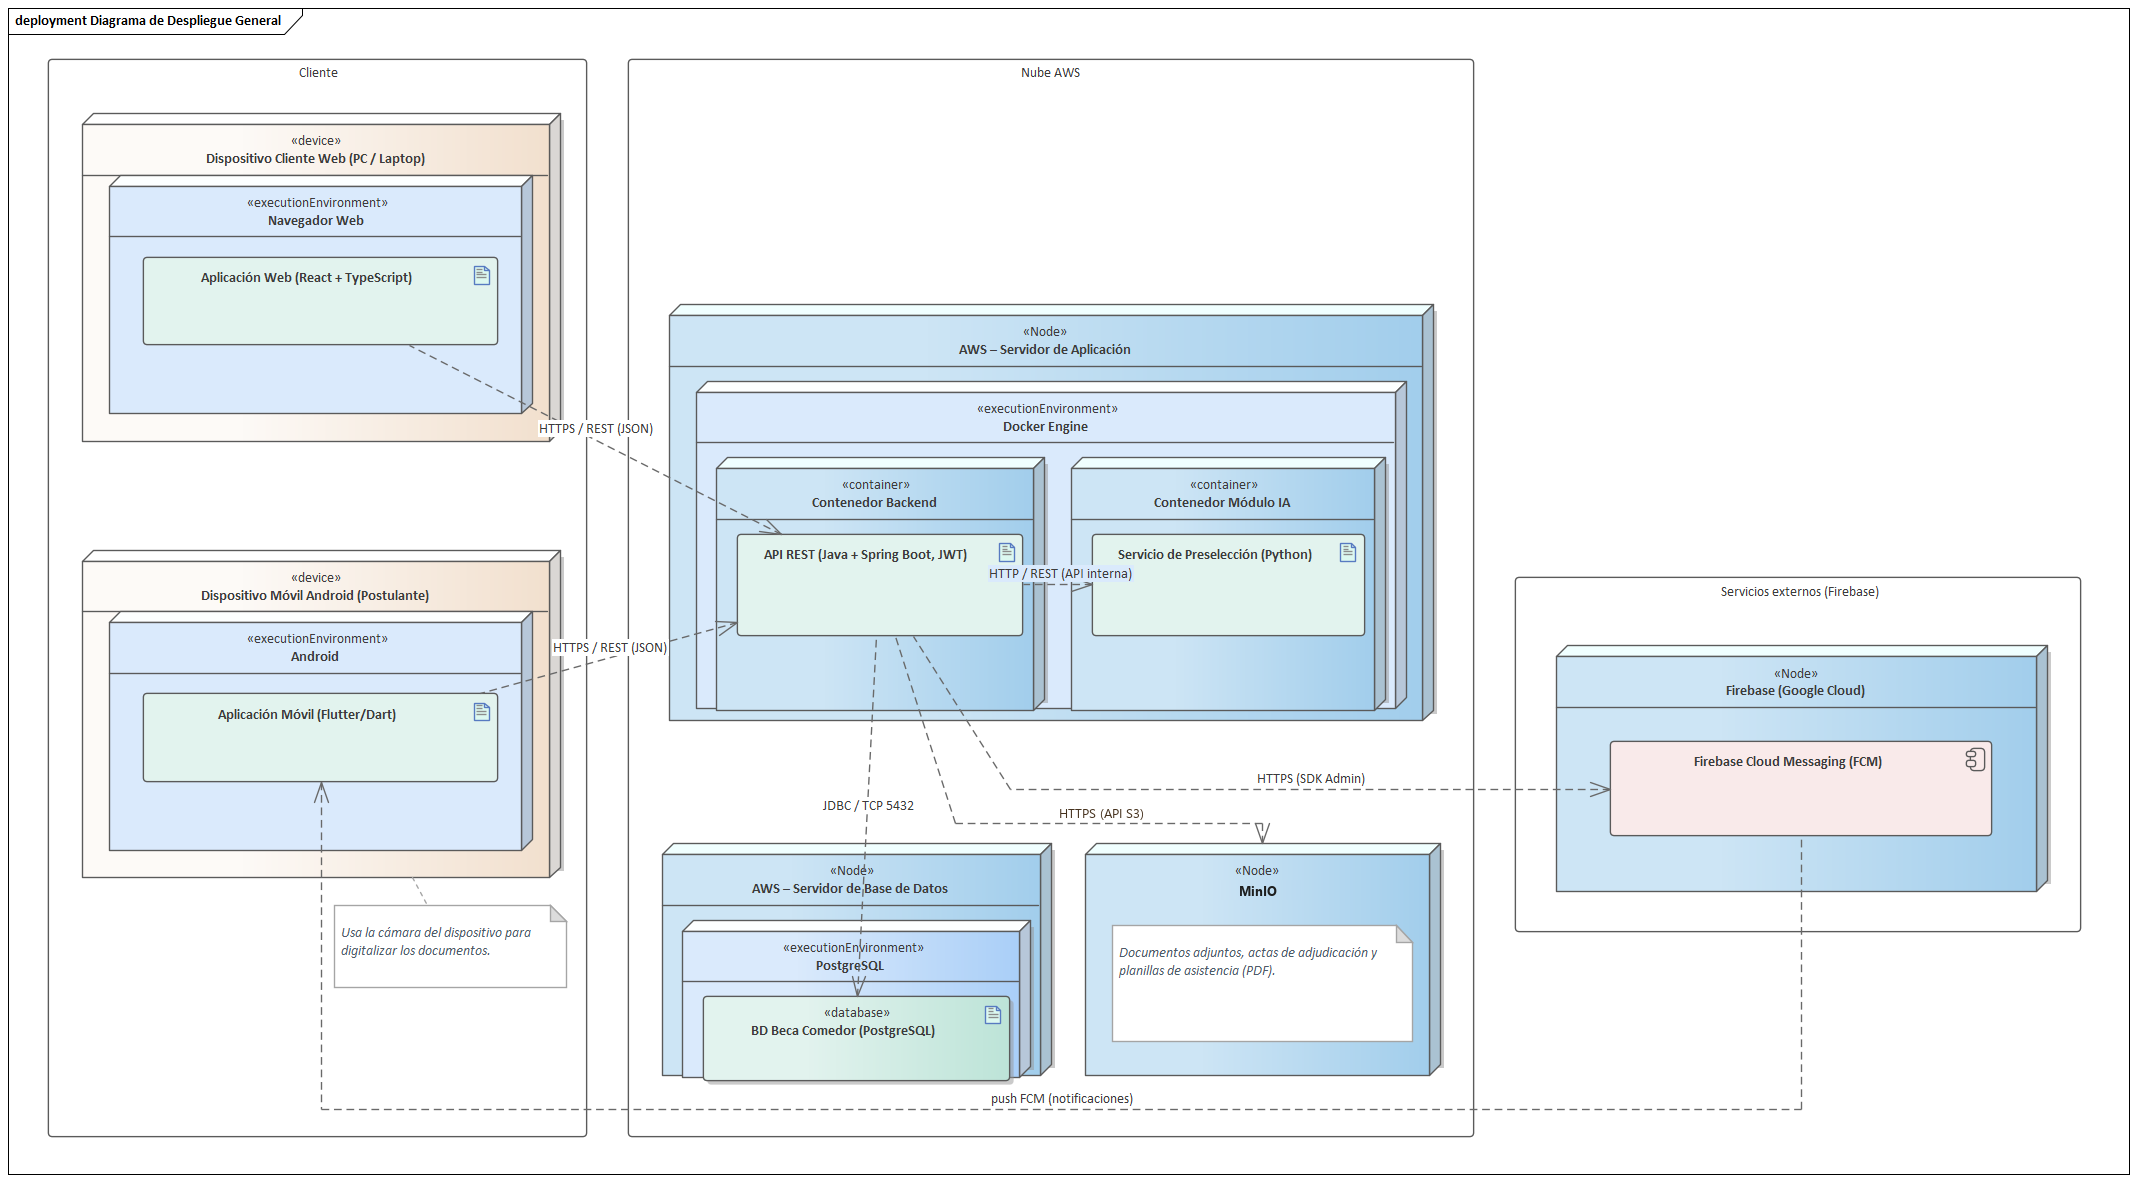
\includegraphics[width=\linewidth,height=0.8\textheight,keepaspectratio]{images/118_Diagrama_Despliegue_General.png}

\smallskip
\noindent\raggedright\textit{Nota.} Elaboración propia.
\end{figure}
\end{landscape}

\subsubsection{7.1.2. Diseño Lógico}\label{sec:cap7_diseno_logico}

El diseño lógico describe la organización interna del sistema en capas y paquetes, independientemente de los nodos físicos en los que se ejecuta (sección~\ref{sec:cap7_diseno_fisico}). Se representa mediante diagramas de paquetes del Lenguaje Unificado de Modelado, en los que cada capa agrupa los paquetes con responsabilidades afines y las dependencias de uso (\textit{use}) se dirigen de las capas superiores hacia las inferiores \parencite{booch2005uml, rumbaugh2004uml}. Este criterio es coherente con el encapsulamiento de los casos de uso en paquetes realizado en el análisis (sección~\ref{sec:cap6_encapsulamiento_cu}), de modo que los seis paquetes funcionales identificados se conservan como módulos de la capa de negocio \parencite{jacobson1999unified}.

\paragraph{Arquitectura lógica general.} La Figura~\ref{fig:diseno_logico_general} presenta la arquitectura lógica general del sistema, organizada en cuatro capas y un paquete de aspectos transversales. La capa de presentación contiene la aplicación web (React y TypeScript) y la aplicación móvil (Flutter), con las que interactúan los usuarios del sistema. La capa de servicios expone la API REST de Spring Boot, con sus controladores y objetos de transferencia de datos, y el mecanismo de autenticación y autorización, que emite y verifica los tokens JWT y aplica el rol del usuario. La capa de negocio agrupa los módulos de cuentas y acceso, convocatoria y postulación, auditoría y adjudicación, becados y asistencia, reportes y trazabilidad, y preselección con inteligencia artificial; este último se implementa en Python como servicio independiente que se consume mediante una API interna. La capa de acceso a datos reúne los repositorios (JPA e Hibernate) y los agentes de servicios externos, que a su vez dependen de la base de datos PostgreSQL y de los servicios externos (notificaciones push, almacenamiento de archivos y módulo de inteligencia artificial). Finalmente, los aspectos transversales (seguridad, bitácora y auditoría de acciones, manejo de errores y validaciones, y notificaciones) son utilizados por todas las capas.

\begin{landscape}
\begin{figure}[p]
\caption{Arquitectura lógica general del sistema en capas}
\label{fig:diseno_logico_general}
\centering
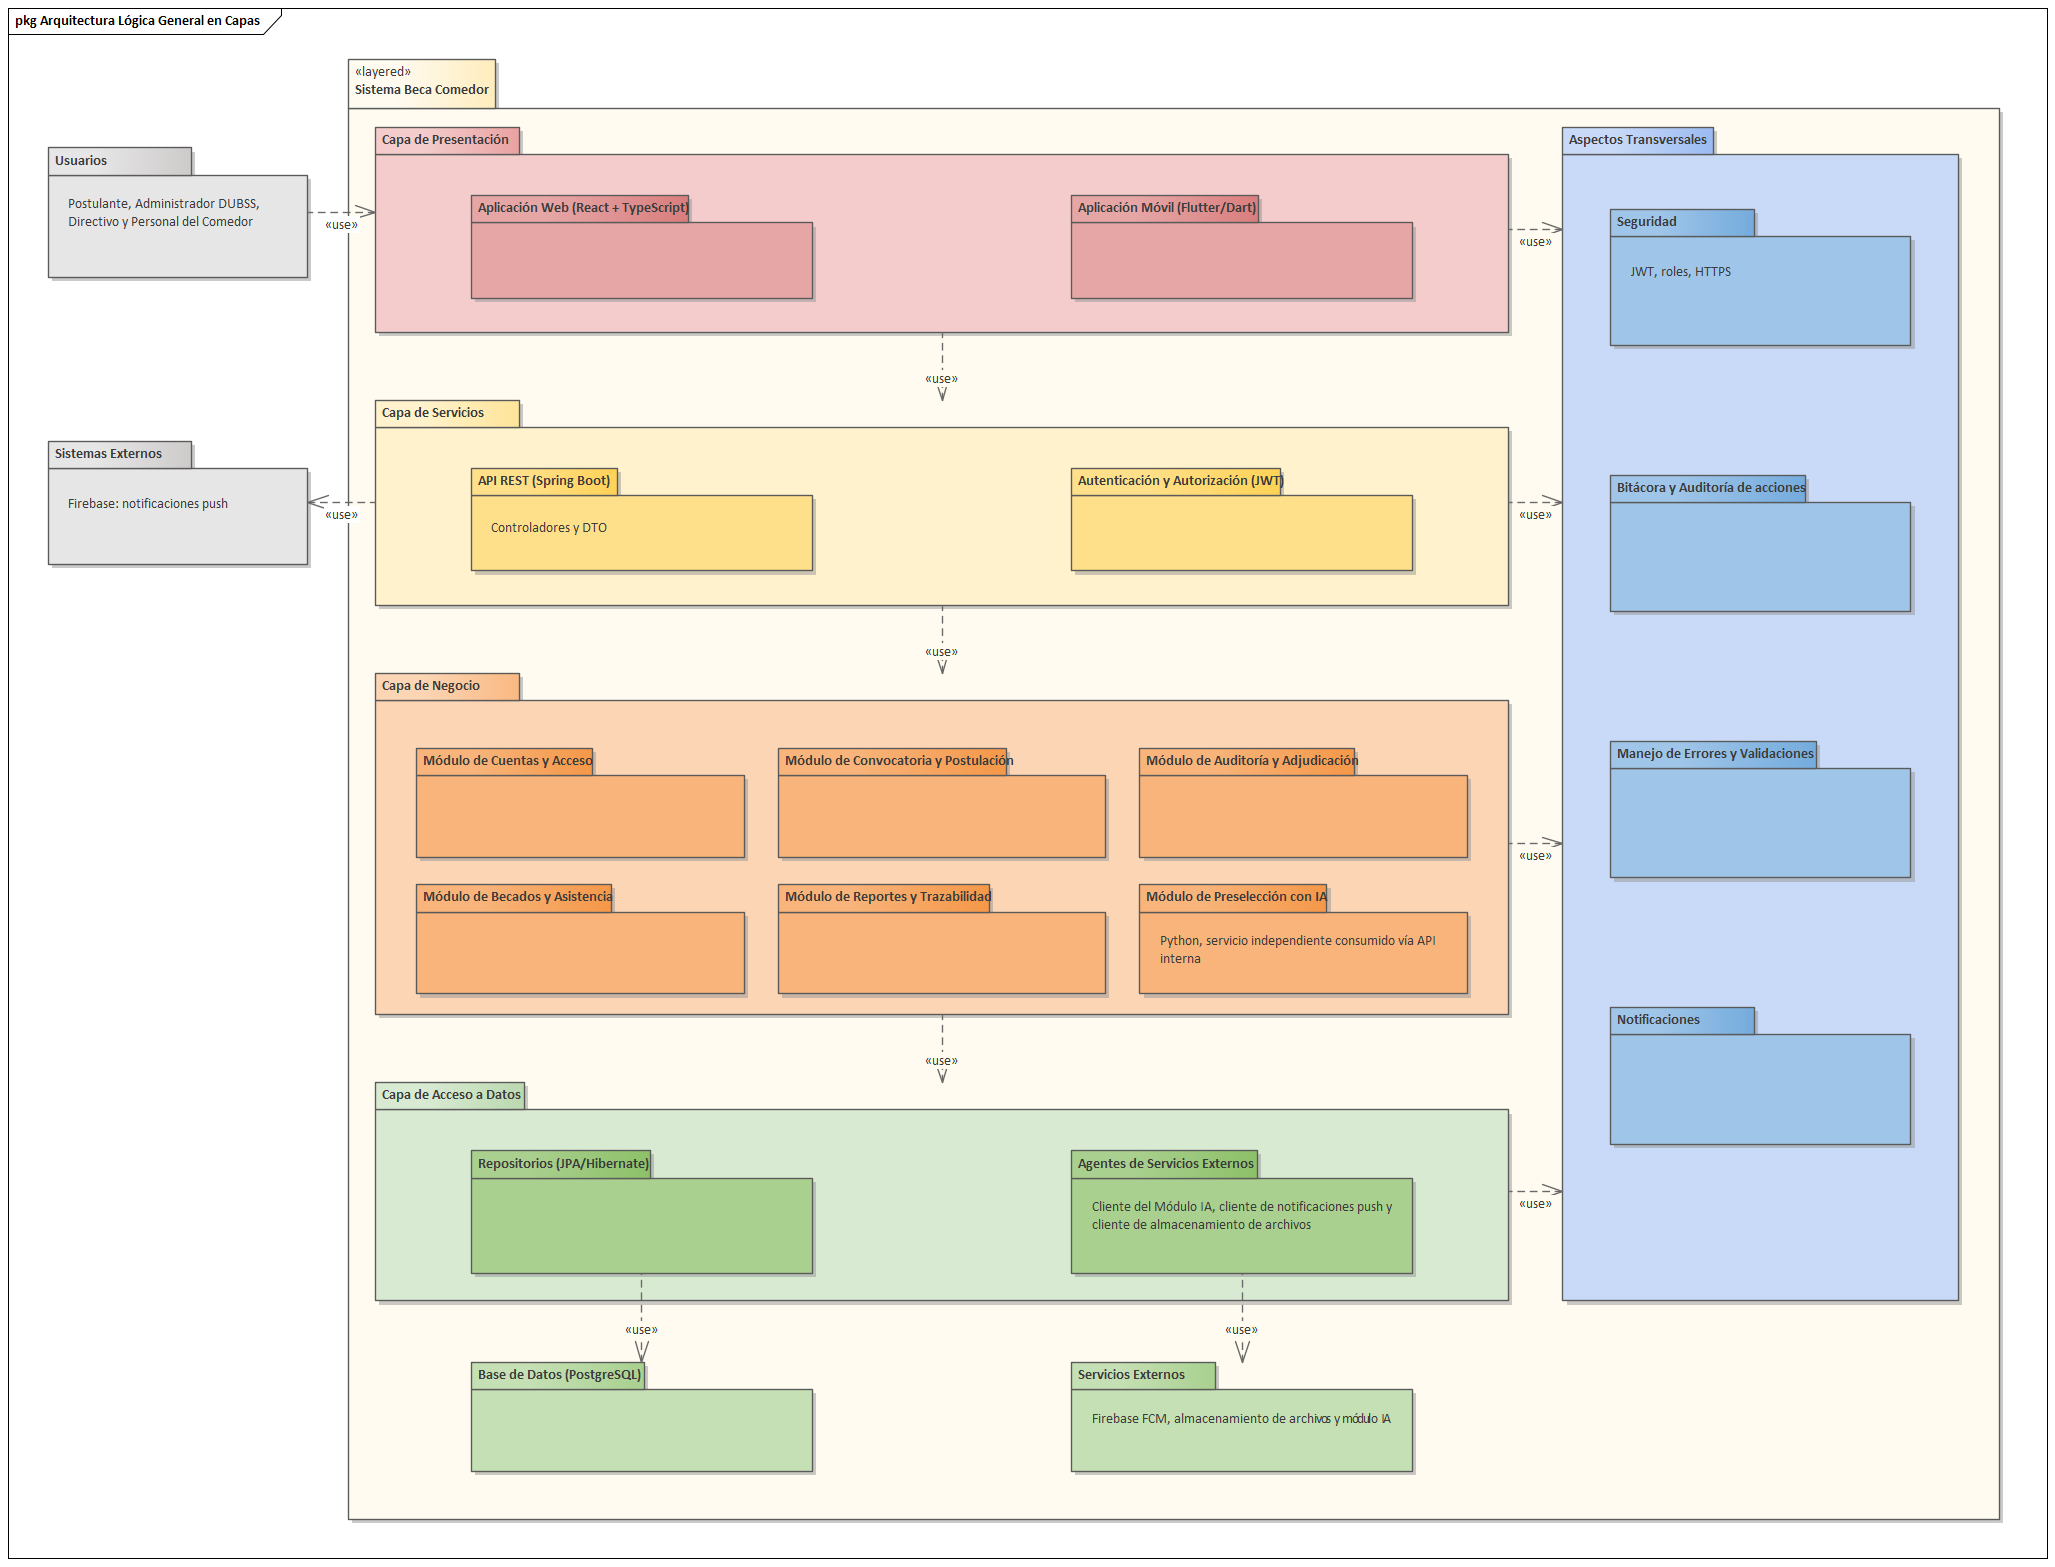
\includegraphics[width=\linewidth,height=0.8\textheight,keepaspectratio]{images/119_Diseno_Logico_Arquitectura_General.png}

\smallskip
\noindent\raggedright\textit{Nota.} Elaboración propia.
\end{figure}
\end{landscape}

\paragraph{Arquitectura lógica del \textit{backend}.} La Figura~\ref{fig:diseno_logico_backend} detalla la organización del \textit{backend} desarrollado con Spring Boot. La capa de presentación (API) contiene los controladores REST y los objetos de transferencia de datos con sus mapeadores; los controladores invocan a los servicios de la capa de lógica de aplicación, que se organizan según los seis paquetes funcionales: cuentas y acceso (P1), convocatoria y postulación (P2), preselección con IA (P3), auditoría y adjudicación (P4), becados y asistencia (P5), y reportes y trazabilidad (P6). Entre estos paquetes existen dependencias que reflejan el flujo del proceso: los servicios de becados y asistencia utilizan los de auditoría y adjudicación, estos utilizan los de convocatoria y postulación, y estos últimos los de preselección con IA. Los servicios operan sobre la capa de dominio, que contiene las entidades y las enumeraciones (por ejemplo, el estado de la postulación), y acceden a la capa de persistencia, conformada por los repositorios JPA, el cliente del módulo de inteligencia artificial y los clientes de notificaciones push y de almacenamiento de archivos. Los repositorios acceden a la base de datos PostgreSQL, y el paquete de seguridad y bitácora es utilizado por todas las capas.

\begin{landscape}
\begin{figure}[p]
\caption{Arquitectura lógica del \textit{backend} (Spring Boot)}
\label{fig:diseno_logico_backend}
\centering
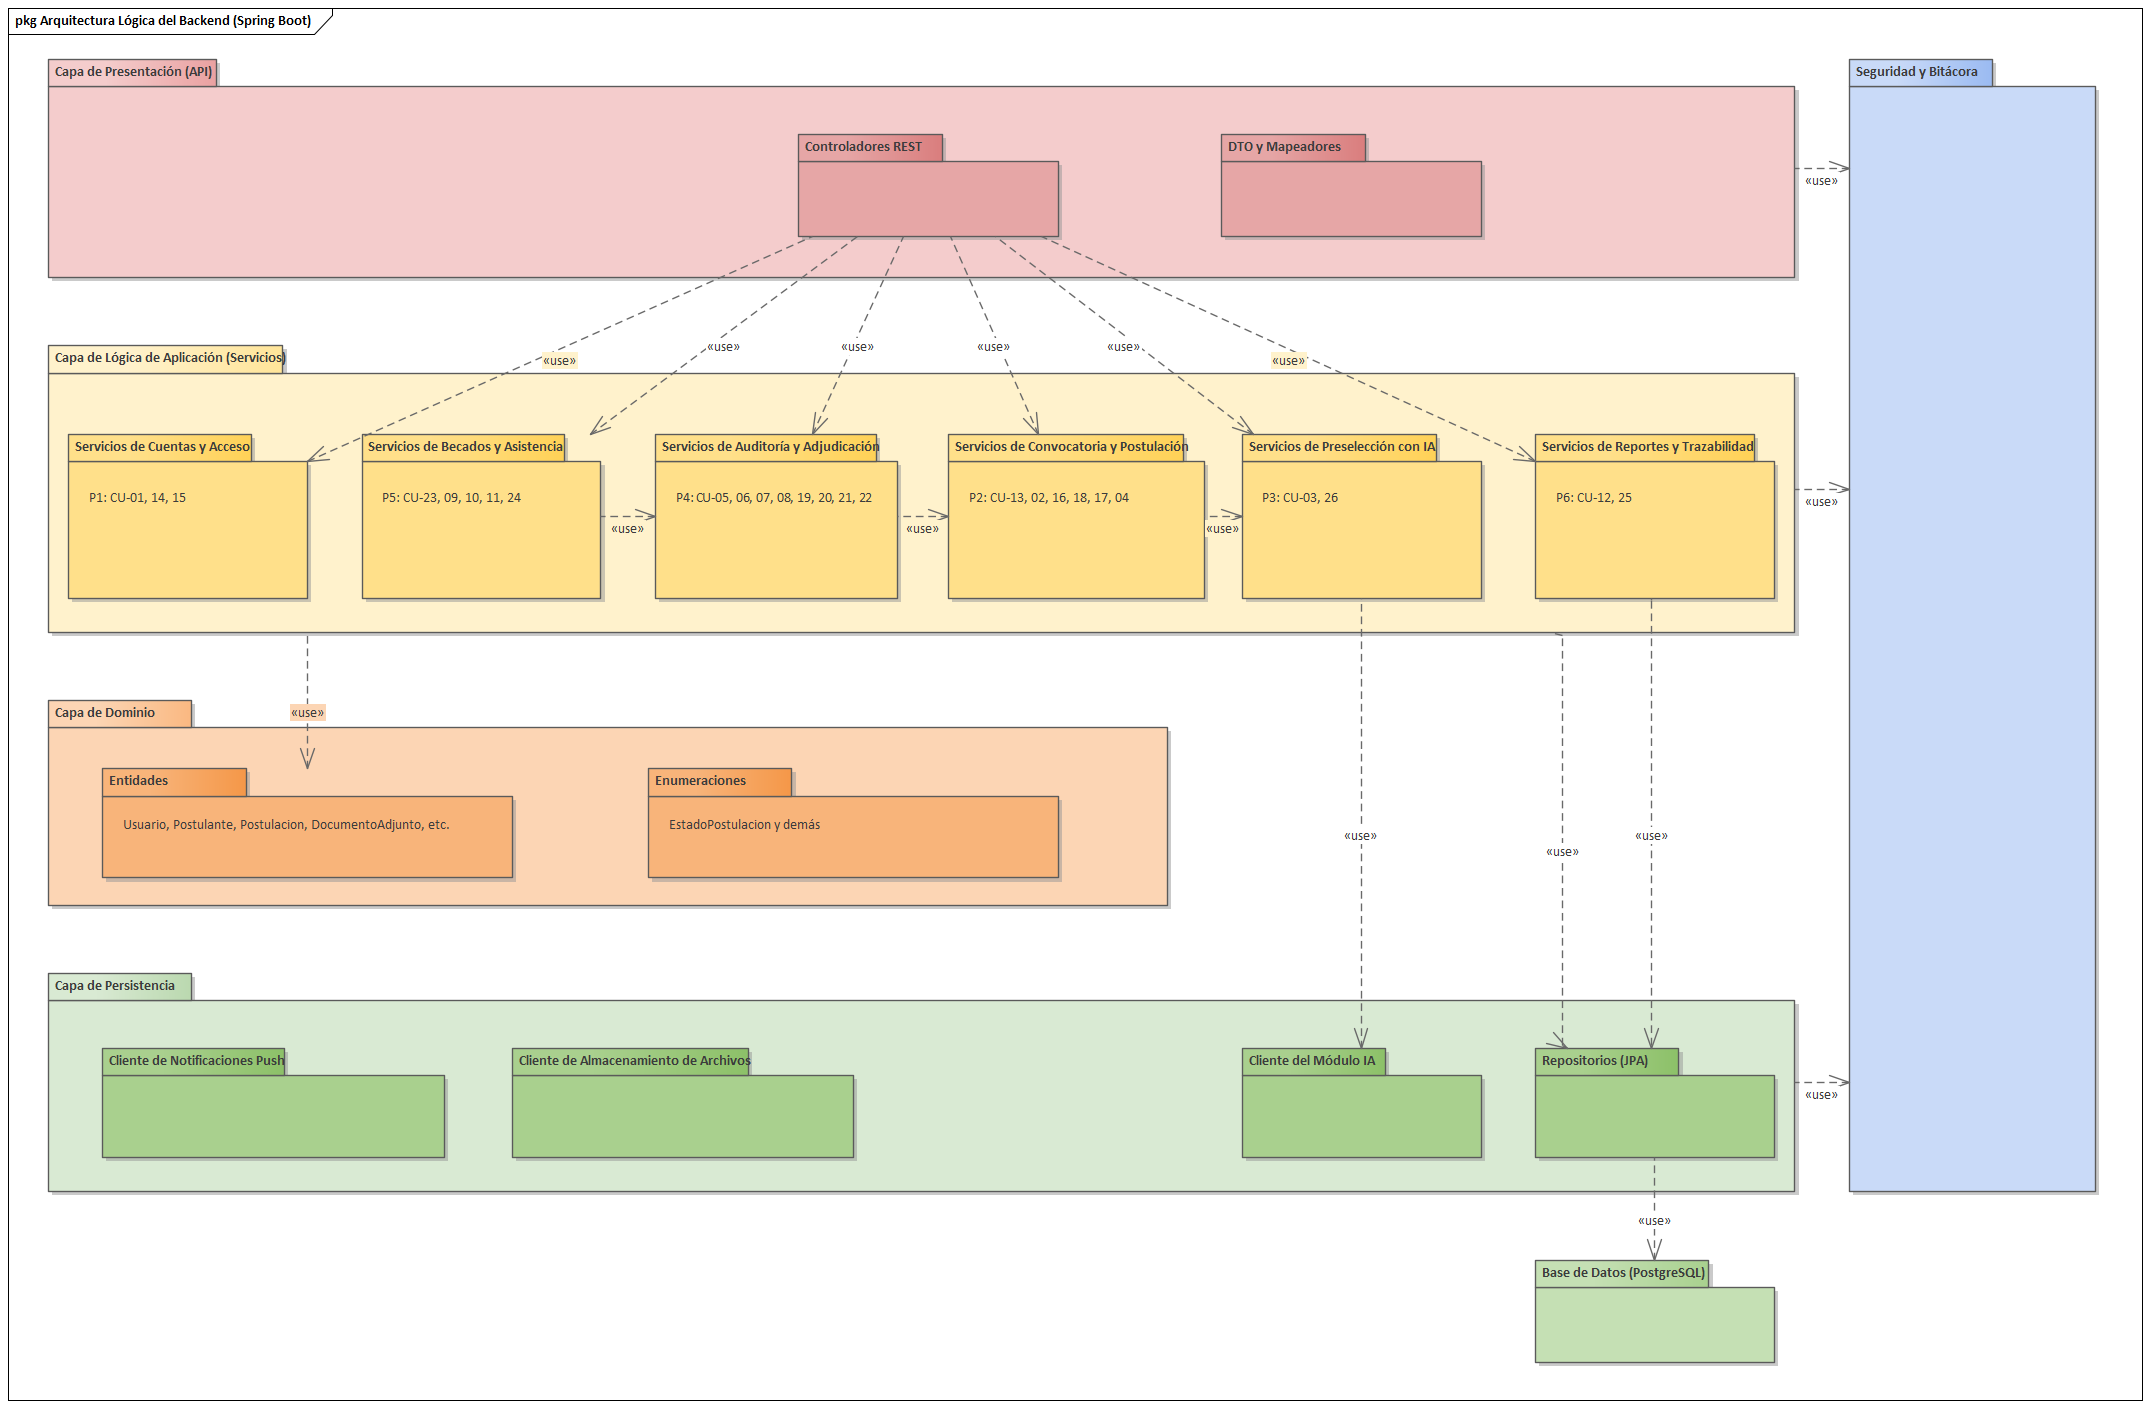
\includegraphics[width=\linewidth,height=0.8\textheight,keepaspectratio]{images/120_Diseno_Logico_Backend.png}

\smallskip
\noindent\raggedright\textit{Nota.} Elaboración propia. P1 a P6 corresponden a los paquetes de casos de uso definidos en el análisis.
\end{figure}
\end{landscape}

% ------------------------------------------------------------------------------
% 7.2. DIAGRAMA DE CLASE
% ------------------------------------------------------------------------------
\wfa{\wn{7}.2. Diagrama de Clase}\label{sec:cap7_diagrama_clase}

El diagrama de clases de diseño integra las clases de entidad identificadas en el análisis de los casos de uso (Capítulo 6) y las refina con sus atributos, tipos de datos, operaciones y relaciones de asociación, composición y herencia, expresadas en el Lenguaje Unificado de Modelado \parencite{booch2005uml}. Las clases representan la información persistente del dominio de la Beca Comedor y se corresponden con las tablas del diseño de datos (sección~\ref{sec:cap7_diseno_datos}); los valores admitidos para los estados y tipos se modelan como enumeraciones.

Todas las clases, excepto \textit{Postulante}, que hereda de \textit{Usuario}, heredan de la clase abstracta \textit{EntidadBase}, que aporta el identificador interno, el código público (UUID) y las fechas de creación, actualización y eliminación lógica; las líneas de esa herencia se omiten en el diagrama para no saturarlo. La Figura~\ref{fig:diagrama_clases} presenta el diagrama de clases del sistema.

\begin{landscape}
\begin{figure}[p]
\caption{Diagrama de clases del sistema}
\label{fig:diagrama_clases}
\centering
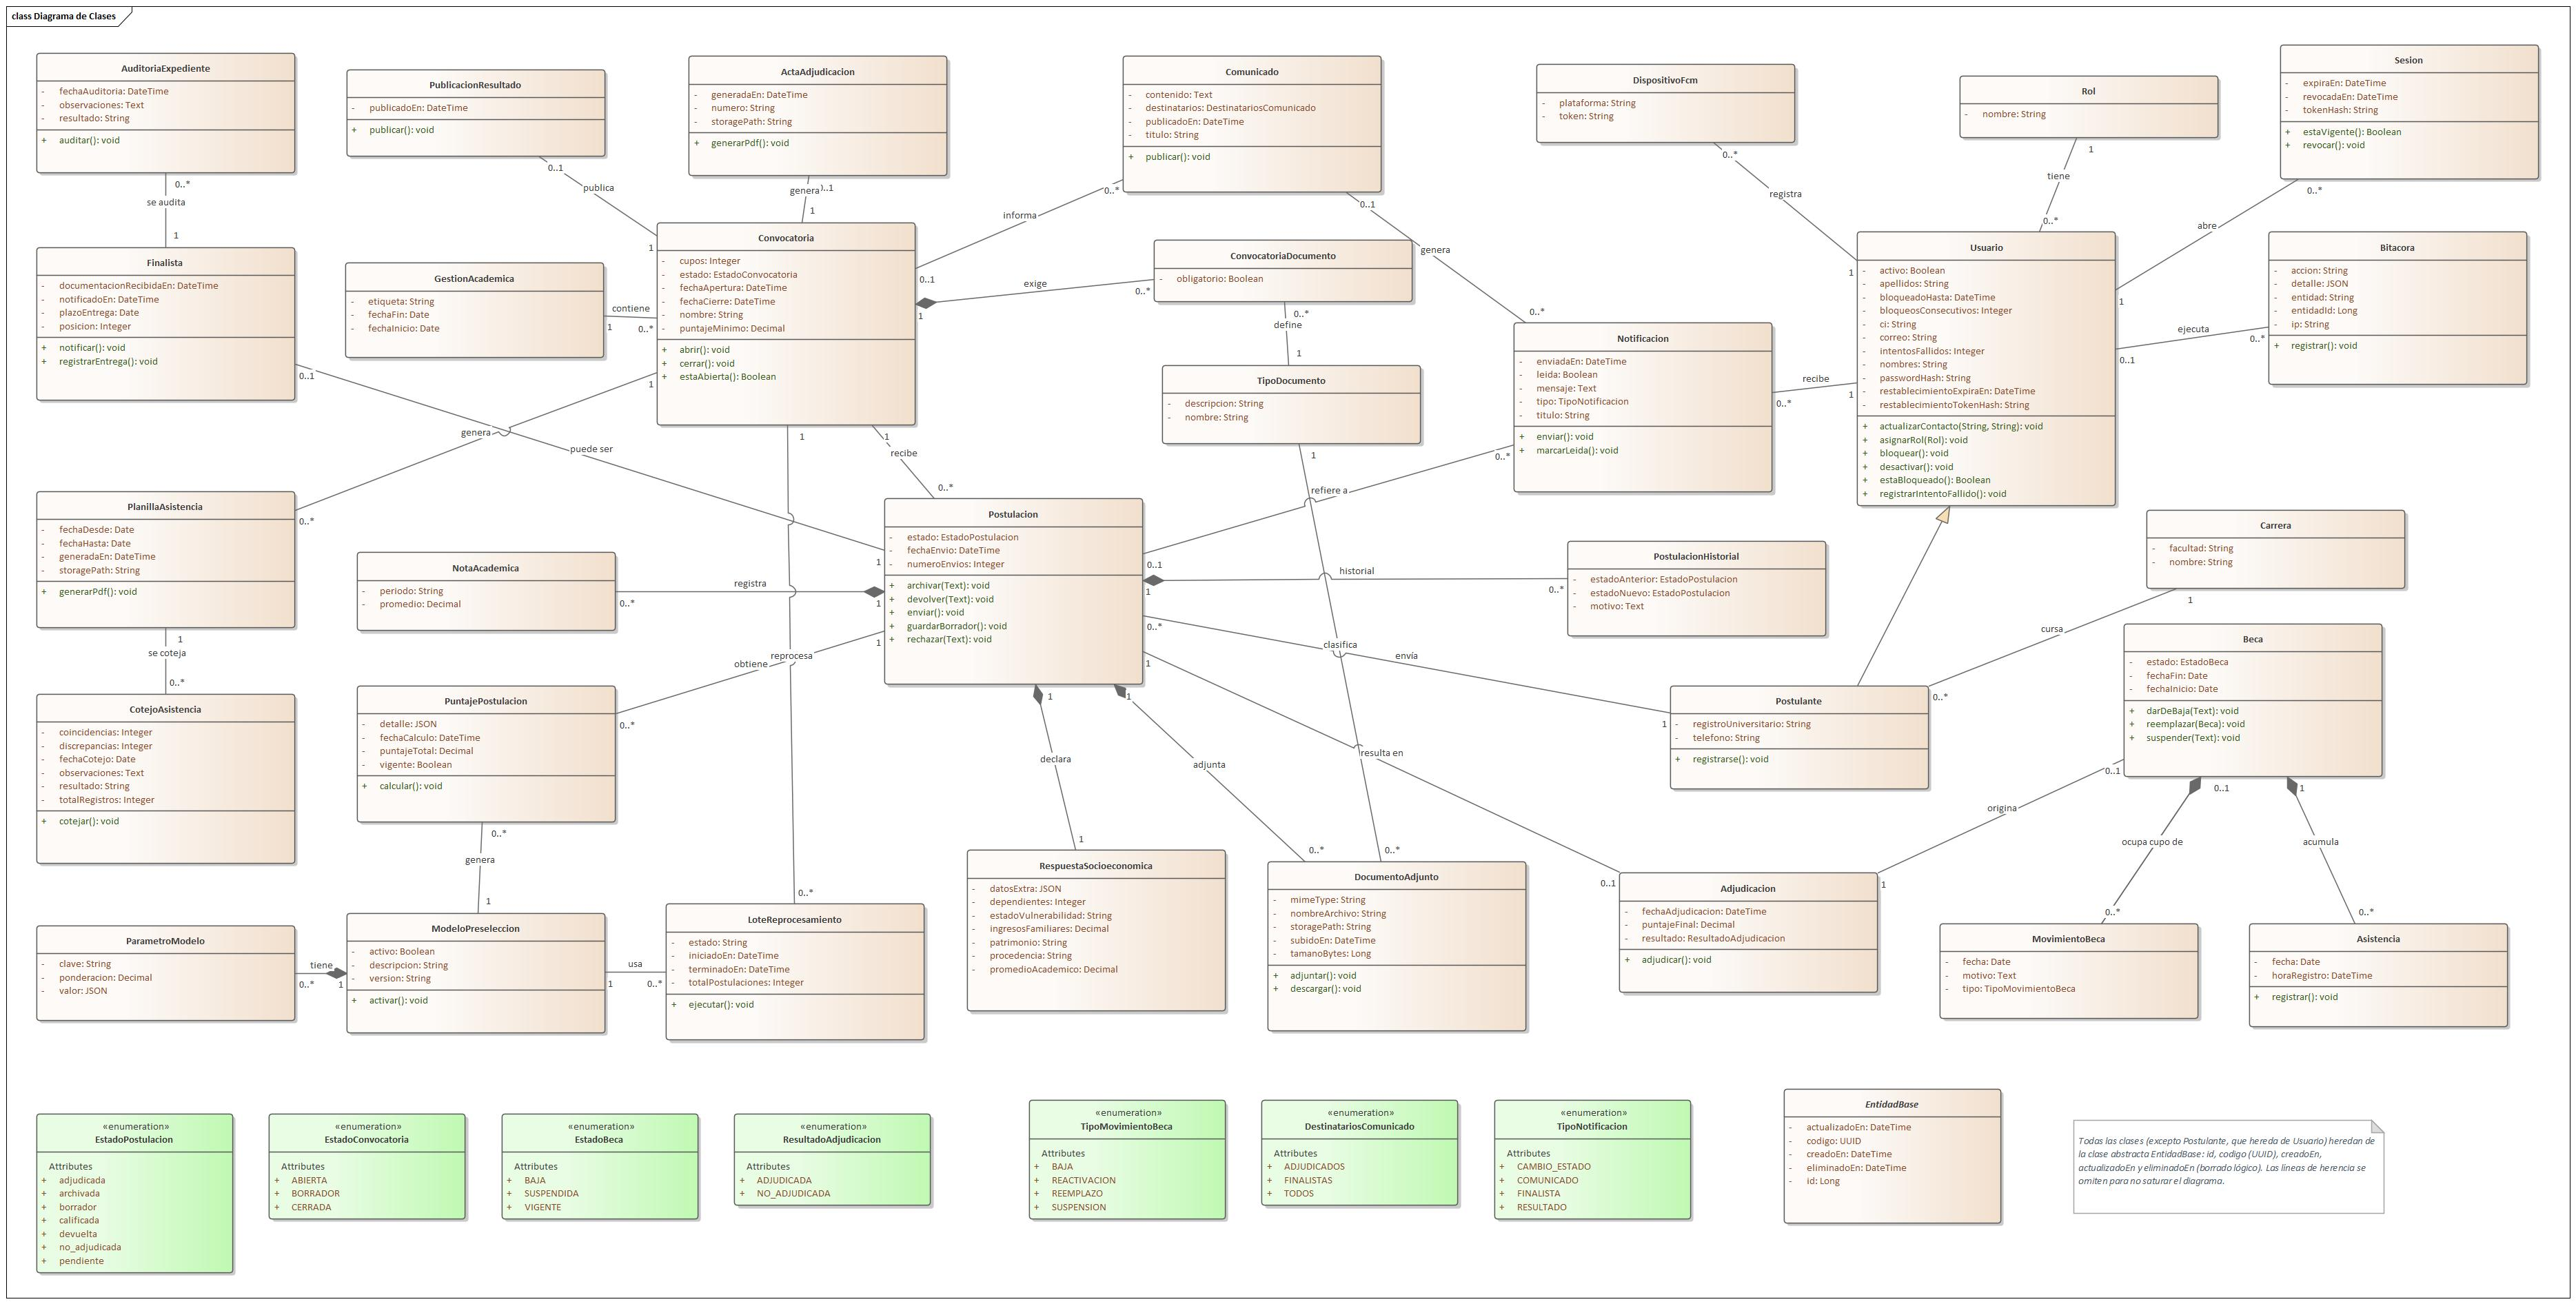
\includegraphics[width=\linewidth,height=0.8\textheight,keepaspectratio]{images/090_Diagrama_de_Clases.jpg}

\smallskip
\noindent\raggedright\textit{Nota.} Elaboración propia.
\end{figure}
\end{landscape}

% ------------------------------------------------------------------------------
% 7.3. DISEÑO DE DATOS
% ------------------------------------------------------------------------------
\wfa{\wn{7}.3. Diseño de Datos}\label{sec:cap7_diseno_datos}

El diseño de datos traduce las clases persistentes del diagrama de clases (sección~\ref{sec:cap7_diagrama_clase}) a un modelo relacional implementado en PostgreSQL. El modelo consta de 31 tablas agrupadas según los seis paquetes del análisis: Cuentas y acceso (4), Convocatoria y postulación (9), Preselección con IA (4), Auditoría y adjudicación (8), Becados y asistencia (5) y Reportes y trazabilidad (1). Los nombres de tablas y columnas se escriben en minúsculas, en singular y separados por guion bajo; cada tabla tiene una clave primaria interna \textit{id} y las claves foráneas se nombran \textit{\textless{}tabla\textgreater{}\_id}.

Todas las tablas incorporan cuatro columnas comunes: \textit{codigo\_\textless{}tabla\textgreater{}}, un identificador público UUID versión 7, único y no nulo, que es el único identificador que se expone a la API y a los clientes web y móvil; \textit{creado\_en} y \textit{actualizado\_en}, que registran la fecha y hora de creación y de la última modificación; y \textit{eliminado\_en}, que implementa el borrado lógico, de modo que ningún registro se elimina físicamente. Las contraseñas no se almacenan en la base de datos, pues las gestiona Firebase Authentication, y los archivos se guardan en Firebase Storage, del que la base de datos solo conserva la ruta.

\wfb{\wn{7}.3.1. Diseño de Datos Lógico}\label{sec:cap7_datos_logico}

\wfc{\wn{7}.3.1.1. Diseño lógico de la Base de Datos.}\label{sec:cap7_logico_bd}
El diseño lógico de la base de datos representa cada tabla con sus columnas, tipos de datos, claves primarias (PK), claves foráneas (FK) y restricciones de unicidad (UQ), así como las relaciones y cardinalidades entre las tablas. La Figura~\ref{fig:diseno_logico_bd} presenta el diagrama del diseño lógico.

\begin{figure}[H]
\caption{Diseño lógico de la base de datos}
\label{fig:diseno_logico_bd}
\centering
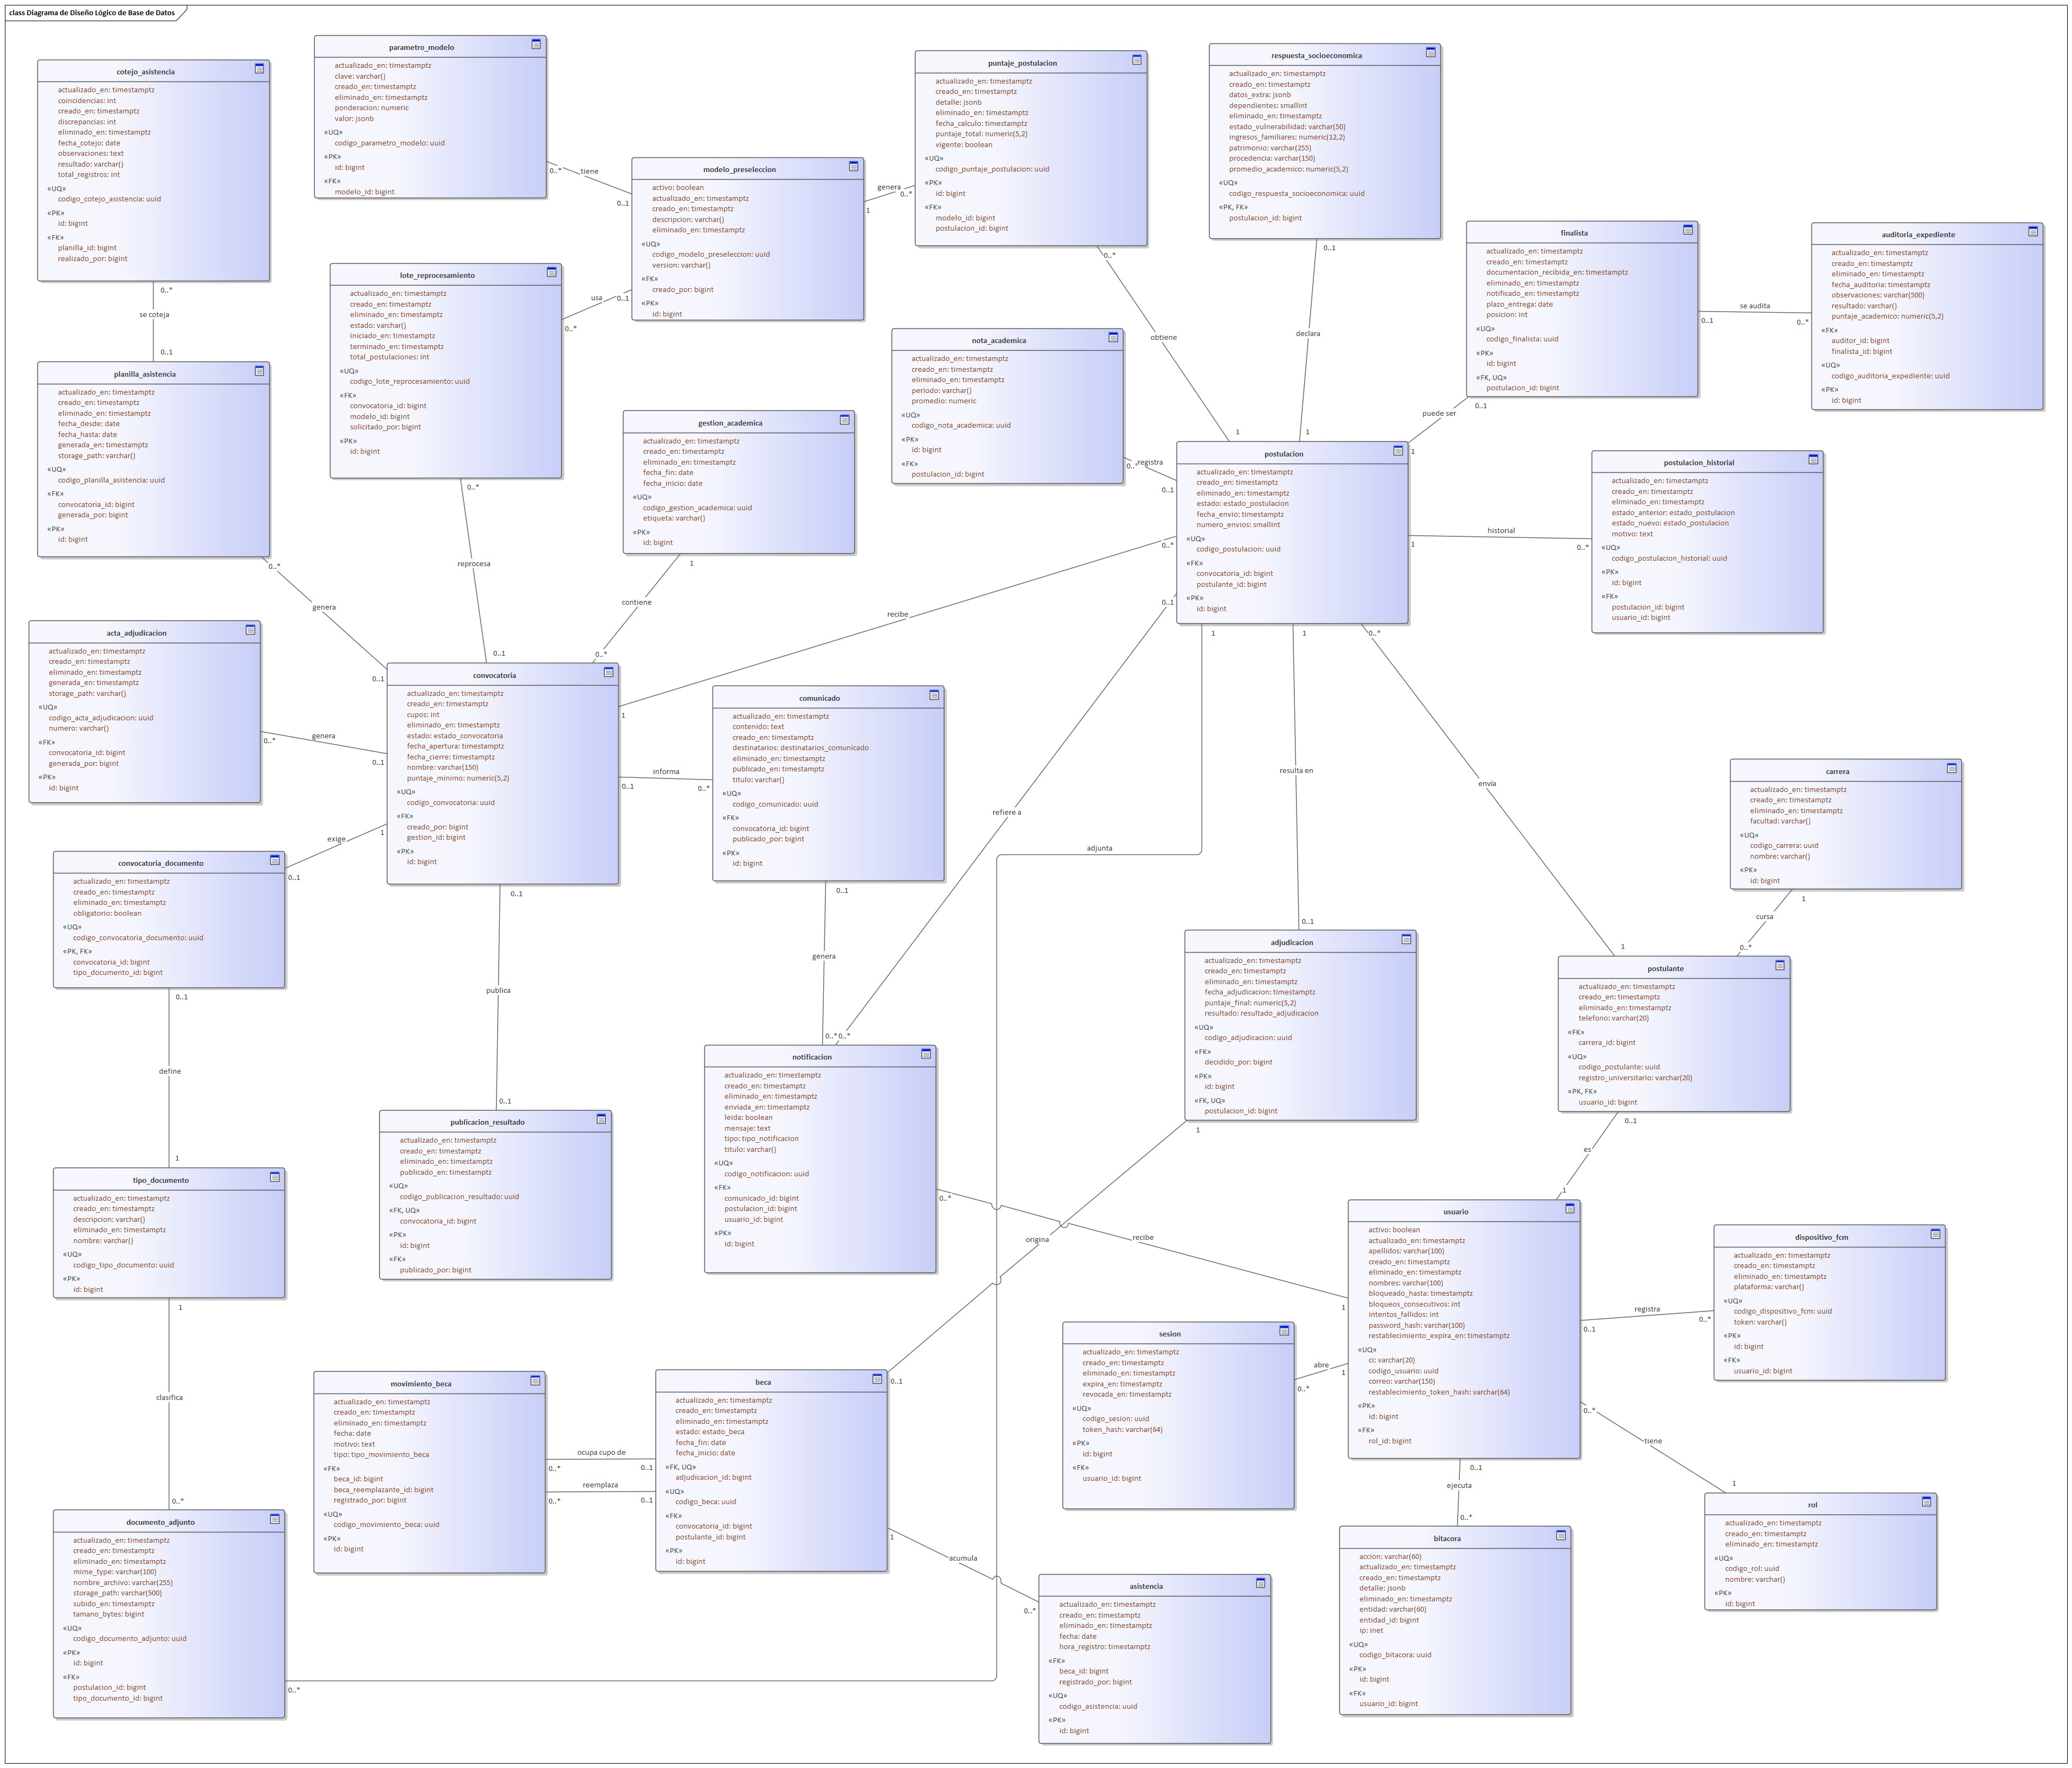
\includegraphics[width=\textwidth,height=0.8\textheight,keepaspectratio]{images/091_Diseno_Logico_Base_de_Datos.jpg}

\smallskip
\noindent\raggedright\textit{Nota.} Elaboración propia.
\end{figure}

\wfc{\wn{7}.3.1.2. Mapeo.}\label{sec:cap7_mapeo}
El mapeo presenta, para cada una de las 31 tablas del diseño lógico, sus atributos y el tipo de dato asignado a cada uno, indicando entre paréntesis las claves primarias (PK), foráneas (FK) y únicas (UQ). Las tablas se presentan agrupadas por paquete, en el mismo orden del diseño lógico.

% ------------------------------------------------------------------------------
% 7.3.1.2. MAPEO (generado a partir del diagrama lógico de la base de datos)
% ------------------------------------------------------------------------------

\begin{table}[H]
\caption{Mapeo de la tabla rol}
\label{tab:mapeo_rol}
\centering
\footnotesize\linespread{1}\selectfont
\renewcommand{\arraystretch}{1.3}
\begin{tabular}{*{5}{>{\centering\arraybackslash}p{2.85cm}}}
\toprule
\textbf{id (PK)} & \textbf{nombre (UQ)} & \textbf{codigo\_\allowbreak{}rol (UQ)} & \textbf{creado\_\allowbreak{}en} & \textbf{actualizado\_\allowbreak{}en} \\
\midrule
bigint & varchar(50) & uuid & timestamptz & timestamptz \\
\bottomrule
\end{tabular}

\vspace{14pt}
\begin{tabular}{*{5}{>{\centering\arraybackslash}p{2.85cm}}}
\toprule
\textbf{eliminado\_\allowbreak{}en} &  &  &  &  \\
\midrule
timestamptz &  &  &  &  \\
\bottomrule
\end{tabular}

\smallskip
\noindent\raggedright\textit{Nota.} Elaboración propia.
\end{table}

\begin{table}[H]
\caption{Mapeo de la tabla usuario}
\label{tab:mapeo_usuario}
\centering
\footnotesize\linespread{1}\selectfont
\renewcommand{\arraystretch}{1.3}
\begin{tabular}{*{5}{>{\centering\arraybackslash}p{2.85cm}}}
\toprule
\textbf{id (PK)} & \textbf{ci (UQ)} & \textbf{correo (UQ)} & \textbf{nombres} & \textbf{apellidos} \\
\midrule
bigint & varchar(20) & varchar(150) & varchar(100) & varchar(100) \\
\bottomrule
\end{tabular}

\vspace{14pt}
\begin{tabular}{*{5}{>{\centering\arraybackslash}p{2.85cm}}}
\toprule
\textbf{password\_\allowbreak{}hash} & \textbf{activo} & \textbf{rol\_\allowbreak{}id (FK)} & \textbf{codigo\_\allowbreak{}usuario (UQ)} & \textbf{intentos\_\allowbreak{}fallidos} \\
\midrule
varchar(100) & boolean & bigint & uuid & integer \\
\bottomrule
\end{tabular}

\vspace{14pt}
\begin{tabular}{*{5}{>{\centering\arraybackslash}p{2.85cm}}}
\toprule
\textbf{bloqueos\_\allowbreak{}consecutivos} & \textbf{bloqueado\_\allowbreak{}hasta} & \textbf{creado\_\allowbreak{}en} & \textbf{actualizado\_\allowbreak{}en} & \textbf{eliminado\_\allowbreak{}en} \\
\midrule
integer & timestamptz & timestamptz & timestamptz & timestamptz \\
\bottomrule
\end{tabular}

\smallskip
\noindent\raggedright\textit{Nota.} Elaboración propia.
\end{table}

\begin{table}[H]
\caption{Mapeo de la tabla carrera}
\label{tab:mapeo_carrera}
\centering
\footnotesize\linespread{1}\selectfont
\renewcommand{\arraystretch}{1.3}
\begin{tabular}{*{5}{>{\centering\arraybackslash}p{2.85cm}}}
\toprule
\textbf{id (PK)} & \textbf{nombre (UQ)} & \textbf{facultad} & \textbf{codigo\_\allowbreak{}carrera (UQ)} & \textbf{creado\_\allowbreak{}en} \\
\midrule
bigint & varchar(150) & varchar(150) & uuid & timestamptz \\
\bottomrule
\end{tabular}

\vspace{14pt}
\begin{tabular}{*{5}{>{\centering\arraybackslash}p{2.85cm}}}
\toprule
\textbf{actualizado\_\allowbreak{}en} & \textbf{eliminado\_\allowbreak{}en} &  &  &  \\
\midrule
timestamptz & timestamptz &  &  &  \\
\bottomrule
\end{tabular}

\smallskip
\noindent\raggedright\textit{Nota.} Elaboración propia.
\end{table}

\begin{table}[H]
\caption{Mapeo de la tabla sesion}
\label{tab:mapeo_sesion}
\centering
\footnotesize\linespread{1}\selectfont
\renewcommand{\arraystretch}{1.3}
\begin{tabular}{*{5}{>{\centering\arraybackslash}p{2.85cm}}}
\toprule
\textbf{id (PK)} & \textbf{usuario\_\allowbreak{}id (FK)} & \textbf{codigo\_\allowbreak{}sesion (UQ)} & \textbf{token\_\allowbreak{}hash (UQ)} & \textbf{expira\_\allowbreak{}en} \\
\midrule
bigint & bigint & uuid & varchar(64) & timestamptz \\
\bottomrule
\end{tabular}

\vspace{14pt}
\begin{tabular}{*{5}{>{\centering\arraybackslash}p{2.85cm}}}
\toprule
\textbf{revocada\_\allowbreak{}en} & \textbf{creado\_\allowbreak{}en} & \textbf{actualizado\_\allowbreak{}en} & \textbf{eliminado\_\allowbreak{}en} &  \\
\midrule
timestamptz & timestamptz & timestamptz & timestamptz &  \\
\bottomrule
\end{tabular}

\smallskip
\noindent\raggedright\textit{Nota.} Elaboración propia.
\end{table}

\begin{table}[H]
\caption{Mapeo de la tabla postulante}
\label{tab:mapeo_postulante}
\centering
\footnotesize\linespread{1}\selectfont
\renewcommand{\arraystretch}{1.3}
\begin{tabular}{*{5}{>{\centering\arraybackslash}p{2.85cm}}}
\toprule
\textbf{usuario\_\allowbreak{}id (PK, FK)} & \textbf{carrera\_\allowbreak{}id (FK)} & \textbf{registro\_\allowbreak{}universitario (UQ)} & \textbf{telefono} & \textbf{codigo\_\allowbreak{}postulante (UQ)} \\
\midrule
bigint & bigint & varchar(20) & varchar(20) & uuid \\
\bottomrule
\end{tabular}

\vspace{14pt}
\begin{tabular}{*{5}{>{\centering\arraybackslash}p{2.85cm}}}
\toprule
\textbf{creado\_\allowbreak{}en} & \textbf{actualizado\_\allowbreak{}en} & \textbf{eliminado\_\allowbreak{}en} &  &  \\
\midrule
timestamptz & timestamptz & timestamptz &  &  \\
\bottomrule
\end{tabular}

\smallskip
\noindent\raggedright\textit{Nota.} Elaboración propia.
\end{table}

\begin{table}[H]
\caption{Mapeo de la tabla gestion\_\allowbreak{}academica}
\label{tab:mapeo_gestion_academica}
\centering
\footnotesize\linespread{1}\selectfont
\renewcommand{\arraystretch}{1.3}
\begin{tabular}{*{5}{>{\centering\arraybackslash}p{2.85cm}}}
\toprule
\textbf{id (PK)} & \textbf{etiqueta (UQ)} & \textbf{fecha\_\allowbreak{}inicio} & \textbf{fecha\_\allowbreak{}fin} & \textbf{codigo\_\allowbreak{}gestion\_\allowbreak{}academica (UQ)} \\
\midrule
bigint & varchar(20) & date & date & uuid \\
\bottomrule
\end{tabular}

\vspace{14pt}
\begin{tabular}{*{5}{>{\centering\arraybackslash}p{2.85cm}}}
\toprule
\textbf{creado\_\allowbreak{}en} & \textbf{actualizado\_\allowbreak{}en} & \textbf{eliminado\_\allowbreak{}en} &  &  \\
\midrule
timestamptz & timestamptz & timestamptz &  &  \\
\bottomrule
\end{tabular}

\smallskip
\noindent\raggedright\textit{Nota.} Elaboración propia.
\end{table}

\begin{table}[H]
\caption{Mapeo de la tabla convocatoria}
\label{tab:mapeo_convocatoria}
\centering
\footnotesize\linespread{1}\selectfont
\renewcommand{\arraystretch}{1.3}
\begin{tabular}{*{5}{>{\centering\arraybackslash}p{2.85cm}}}
\toprule
\textbf{id (PK)} & \textbf{gestion\_\allowbreak{}id (FK)} & \textbf{nombre} & \textbf{fecha\_\allowbreak{}apertura} & \textbf{fecha\_\allowbreak{}cierre} \\
\midrule
bigint & bigint & varchar(150) & timestamptz & timestamptz \\
\bottomrule
\end{tabular}

\vspace{14pt}
\begin{tabular}{*{5}{>{\centering\arraybackslash}p{2.85cm}}}
\toprule
\textbf{cupos} & \textbf{puntaje\_\allowbreak{}minimo} & \textbf{estado} & \textbf{creado\_\allowbreak{}por (FK)} & \textbf{codigo\_\allowbreak{}convocatoria (UQ)} \\
\midrule
integer & numeric(5,2) & estado\_\allowbreak{}convocatoria & bigint & uuid \\
\bottomrule
\end{tabular}

\vspace{14pt}
\begin{tabular}{*{5}{>{\centering\arraybackslash}p{2.85cm}}}
\toprule
\textbf{creado\_\allowbreak{}en} & \textbf{actualizado\_\allowbreak{}en} & \textbf{eliminado\_\allowbreak{}en} &  &  \\
\midrule
timestamptz & timestamptz & timestamptz &  &  \\
\bottomrule
\end{tabular}

\smallskip
\noindent\raggedright\textit{Nota.} Elaboración propia.
\end{table}

\begin{table}[H]
\caption{Mapeo de la tabla tipo\_\allowbreak{}documento}
\label{tab:mapeo_tipo_documento}
\centering
\footnotesize\linespread{1}\selectfont
\renewcommand{\arraystretch}{1.3}
\begin{tabular}{*{5}{>{\centering\arraybackslash}p{2.85cm}}}
\toprule
\textbf{id (PK)} & \textbf{nombre} & \textbf{descripcion} & \textbf{codigo\_\allowbreak{}tipo\_\allowbreak{}documento (UQ)} & \textbf{creado\_\allowbreak{}en} \\
\midrule
bigint & varchar(100) & varchar(255) & uuid & timestamptz \\
\bottomrule
\end{tabular}

\vspace{14pt}
\begin{tabular}{*{5}{>{\centering\arraybackslash}p{2.85cm}}}
\toprule
\textbf{actualizado\_\allowbreak{}en} & \textbf{eliminado\_\allowbreak{}en} &  &  &  \\
\midrule
timestamptz & timestamptz &  &  &  \\
\bottomrule
\end{tabular}

\smallskip
\noindent\raggedright\textit{Nota.} Elaboración propia.
\end{table}

\begin{table}[H]
\caption{Mapeo de la tabla convocatoria\_\allowbreak{}documento}
\label{tab:mapeo_convocatoria_documento}
\centering
\footnotesize\linespread{1}\selectfont
\renewcommand{\arraystretch}{1.3}
\begin{tabular}{*{5}{>{\centering\arraybackslash}p{2.85cm}}}
\toprule
\textbf{convocatoria\_\allowbreak{}id (PK, FK)} & \textbf{tipo\_\allowbreak{}documento\_\allowbreak{}id (PK, FK)} & \textbf{obligatorio} & \textbf{codigo\_\allowbreak{}convocatoria\_\allowbreak{}documento (UQ)} & \textbf{creado\_\allowbreak{}en} \\
\midrule
bigint & bigint & boolean & uuid & timestamptz \\
\bottomrule
\end{tabular}

\vspace{14pt}
\begin{tabular}{*{5}{>{\centering\arraybackslash}p{2.85cm}}}
\toprule
\textbf{actualizado\_\allowbreak{}en} & \textbf{eliminado\_\allowbreak{}en} &  &  &  \\
\midrule
timestamptz & timestamptz &  &  &  \\
\bottomrule
\end{tabular}

\smallskip
\noindent\raggedright\textit{Nota.} Elaboración propia.
\end{table}

\begin{table}[H]
\caption{Mapeo de la tabla postulacion}
\label{tab:mapeo_postulacion}
\centering
\footnotesize\linespread{1}\selectfont
\renewcommand{\arraystretch}{1.3}
\begin{tabular}{*{5}{>{\centering\arraybackslash}p{2.85cm}}}
\toprule
\textbf{id (PK)} & \textbf{postulante\_\allowbreak{}id (FK)} & \textbf{convocatoria\_\allowbreak{}id (FK)} & \textbf{estado} & \textbf{fecha\_\allowbreak{}envio} \\
\midrule
bigint & bigint & bigint & estado\_\allowbreak{}postulacion & timestamptz \\
\bottomrule
\end{tabular}

\vspace{14pt}
\begin{tabular}{*{5}{>{\centering\arraybackslash}p{2.85cm}}}
\toprule
\textbf{numero\_\allowbreak{}envios} & \textbf{codigo\_\allowbreak{}postulacion (UQ)} & \textbf{creado\_\allowbreak{}en} & \textbf{actualizado\_\allowbreak{}en} & \textbf{eliminado\_\allowbreak{}en} \\
\midrule
smallint & uuid & timestamptz & timestamptz & timestamptz \\
\bottomrule
\end{tabular}

\smallskip
\noindent\raggedright\textit{Nota.} Elaboración propia.
\end{table}

\begin{table}[H]
\caption{Mapeo de la tabla respuesta\_\allowbreak{}socioeconomica}
\label{tab:mapeo_respuesta_socioeconomica}
\centering
\footnotesize\linespread{1}\selectfont
\renewcommand{\arraystretch}{1.3}
\begin{tabular}{*{5}{>{\centering\arraybackslash}p{2.85cm}}}
\toprule
\textbf{postulacion\_\allowbreak{}id (PK, FK)} & \textbf{ingresos\_\allowbreak{}familiares} & \textbf{dependientes} & \textbf{procedencia} & \textbf{patrimonio} \\
\midrule
bigint & numeric(12,2) & smallint & varchar(150) & varchar(255) \\
\bottomrule
\end{tabular}

\vspace{14pt}
\begin{tabular}{*{5}{>{\centering\arraybackslash}p{2.85cm}}}
\toprule
\textbf{estado\_\allowbreak{}vulnerabilidad} & \textbf{promedio\_\allowbreak{}academico} & \textbf{datos\_\allowbreak{}extra} & \textbf{codigo\_\allowbreak{}respuesta\_\allowbreak{}socioeconomica (UQ)} & \textbf{creado\_\allowbreak{}en} \\
\midrule
varchar(50) & numeric(5,2) & jsonb & uuid & timestamptz \\
\bottomrule
\end{tabular}

\vspace{14pt}
\begin{tabular}{*{5}{>{\centering\arraybackslash}p{2.85cm}}}
\toprule
\textbf{actualizado\_\allowbreak{}en} & \textbf{eliminado\_\allowbreak{}en} &  &  &  \\
\midrule
timestamptz & timestamptz &  &  &  \\
\bottomrule
\end{tabular}

\smallskip
\noindent\raggedright\textit{Nota.} Elaboración propia.
\end{table}

\begin{table}[H]
\caption{Mapeo de la tabla nota\_\allowbreak{}academica}
\label{tab:mapeo_nota_academica}
\centering
\footnotesize\linespread{1}\selectfont
\renewcommand{\arraystretch}{1.3}
\begin{tabular}{*{5}{>{\centering\arraybackslash}p{2.85cm}}}
\toprule
\textbf{id (PK)} & \textbf{postulacion\_\allowbreak{}id (FK)} & \textbf{periodo} & \textbf{promedio} & \textbf{codigo\_\allowbreak{}nota\_\allowbreak{}academica (UQ)} \\
\midrule
bigint & bigint & varchar(20) & numeric & uuid \\
\bottomrule
\end{tabular}

\vspace{14pt}
\begin{tabular}{*{5}{>{\centering\arraybackslash}p{2.85cm}}}
\toprule
\textbf{creado\_\allowbreak{}en} & \textbf{actualizado\_\allowbreak{}en} & \textbf{eliminado\_\allowbreak{}en} &  &  \\
\midrule
timestamptz & timestamptz & timestamptz &  &  \\
\bottomrule
\end{tabular}

\smallskip
\noindent\raggedright\textit{Nota.} Elaboración propia.
\end{table}

\begin{table}[H]
\caption{Mapeo de la tabla documento\_\allowbreak{}adjunto}
\label{tab:mapeo_documento_adjunto}
\centering
\footnotesize\linespread{1}\selectfont
\renewcommand{\arraystretch}{1.3}
\begin{tabular}{*{5}{>{\centering\arraybackslash}p{2.85cm}}}
\toprule
\textbf{id (PK)} & \textbf{postulacion\_\allowbreak{}id (FK)} & \textbf{tipo\_\allowbreak{}documento\_\allowbreak{}id (FK)} & \textbf{nombre\_\allowbreak{}archivo} & \textbf{storage\_\allowbreak{}path} \\
\midrule
bigint & bigint & bigint & varchar(255) & varchar(500) \\
\bottomrule
\end{tabular}

\vspace{14pt}
\begin{tabular}{*{5}{>{\centering\arraybackslash}p{2.85cm}}}
\toprule
\textbf{mime\_\allowbreak{}type} & \textbf{tamano\_\allowbreak{}bytes} & \textbf{subido\_\allowbreak{}en} & \textbf{codigo\_\allowbreak{}documento\_\allowbreak{}adjunto (UQ)} & \textbf{creado\_\allowbreak{}en} \\
\midrule
varchar(100) & bigint & timestamptz & uuid & timestamptz \\
\bottomrule
\end{tabular}

\vspace{14pt}
\begin{tabular}{*{5}{>{\centering\arraybackslash}p{2.85cm}}}
\toprule
\textbf{actualizado\_\allowbreak{}en} & \textbf{eliminado\_\allowbreak{}en} &  &  &  \\
\midrule
timestamptz & timestamptz &  &  &  \\
\bottomrule
\end{tabular}

\smallskip
\noindent\raggedright\textit{Nota.} Elaboración propia.
\end{table}

\begin{table}[H]
\caption{Mapeo de la tabla postulacion\_\allowbreak{}historial}
\label{tab:mapeo_postulacion_historial}
\centering
\footnotesize\linespread{1}\selectfont
\renewcommand{\arraystretch}{1.3}
\begin{tabular}{*{5}{>{\centering\arraybackslash}p{2.85cm}}}
\toprule
\textbf{id (PK)} & \textbf{postulacion\_\allowbreak{}id (FK)} & \textbf{estado\_\allowbreak{}anterior} & \textbf{estado\_\allowbreak{}nuevo} & \textbf{usuario\_\allowbreak{}id (FK)} \\
\midrule
bigint & bigint & estado\_\allowbreak{}postulacion & estado\_\allowbreak{}postulacion & bigint \\
\bottomrule
\end{tabular}

\vspace{14pt}
\begin{tabular}{*{5}{>{\centering\arraybackslash}p{2.85cm}}}
\toprule
\textbf{motivo} & \textbf{codigo\_\allowbreak{}postulacion\_\allowbreak{}historial (UQ)} & \textbf{creado\_\allowbreak{}en} & \textbf{actualizado\_\allowbreak{}en} & \textbf{eliminado\_\allowbreak{}en} \\
\midrule
text & uuid & timestamptz & timestamptz & timestamptz \\
\bottomrule
\end{tabular}

\smallskip
\noindent\raggedright\textit{Nota.} Elaboración propia.
\end{table}

\begin{table}[H]
\caption{Mapeo de la tabla modelo\_\allowbreak{}preseleccion}
\label{tab:mapeo_modelo_preseleccion}
\centering
\footnotesize\linespread{1}\selectfont
\renewcommand{\arraystretch}{1.3}
\begin{tabular}{*{5}{>{\centering\arraybackslash}p{2.85cm}}}
\toprule
\textbf{id (PK)} & \textbf{version (UQ)} & \textbf{descripcion} & \textbf{activo} & \textbf{creado\_\allowbreak{}por (FK)} \\
\midrule
bigint & varchar(20) & varchar(255) & boolean & bigint \\
\bottomrule
\end{tabular}

\vspace{14pt}
\begin{tabular}{*{5}{>{\centering\arraybackslash}p{2.85cm}}}
\toprule
\textbf{codigo\_\allowbreak{}modelo\_\allowbreak{}preseleccion (UQ)} & \textbf{creado\_\allowbreak{}en} & \textbf{actualizado\_\allowbreak{}en} & \textbf{eliminado\_\allowbreak{}en} &  \\
\midrule
uuid & timestamptz & timestamptz & timestamptz &  \\
\bottomrule
\end{tabular}

\smallskip
\noindent\raggedright\textit{Nota.} Elaboración propia.
\end{table}

\begin{table}[H]
\caption{Mapeo de la tabla parametro\_\allowbreak{}modelo}
\label{tab:mapeo_parametro_modelo}
\centering
\footnotesize\linespread{1}\selectfont
\renewcommand{\arraystretch}{1.3}
\begin{tabular}{*{5}{>{\centering\arraybackslash}p{2.85cm}}}
\toprule
\textbf{id (PK)} & \textbf{modelo\_\allowbreak{}id (FK)} & \textbf{clave} & \textbf{ponderacion} & \textbf{valor} \\
\midrule
bigint & bigint & varchar(100) & numeric & jsonb \\
\bottomrule
\end{tabular}

\vspace{14pt}
\begin{tabular}{*{5}{>{\centering\arraybackslash}p{2.85cm}}}
\toprule
\textbf{codigo\_\allowbreak{}parametro\_\allowbreak{}modelo (UQ)} & \textbf{creado\_\allowbreak{}en} & \textbf{actualizado\_\allowbreak{}en} & \textbf{eliminado\_\allowbreak{}en} &  \\
\midrule
uuid & timestamptz & timestamptz & timestamptz &  \\
\bottomrule
\end{tabular}

\smallskip
\noindent\raggedright\textit{Nota.} Elaboración propia.
\end{table}

\begin{table}[H]
\caption{Mapeo de la tabla puntaje\_\allowbreak{}postulacion}
\label{tab:mapeo_puntaje_postulacion}
\centering
\footnotesize\linespread{1}\selectfont
\renewcommand{\arraystretch}{1.3}
\begin{tabular}{*{5}{>{\centering\arraybackslash}p{2.85cm}}}
\toprule
\textbf{id (PK)} & \textbf{postulacion\_\allowbreak{}id (FK)} & \textbf{modelo\_\allowbreak{}id (FK)} & \textbf{puntaje\_\allowbreak{}total} & \textbf{detalle} \\
\midrule
bigint & bigint & bigint & numeric(5,2) & jsonb \\
\bottomrule
\end{tabular}

\vspace{14pt}
\begin{tabular}{*{5}{>{\centering\arraybackslash}p{2.85cm}}}
\toprule
\textbf{fecha\_\allowbreak{}calculo} & \textbf{vigente} & \textbf{codigo\_\allowbreak{}puntaje\_\allowbreak{}postulacion (UQ)} & \textbf{creado\_\allowbreak{}en} & \textbf{actualizado\_\allowbreak{}en} \\
\midrule
timestamptz & boolean & uuid & timestamptz & timestamptz \\
\bottomrule
\end{tabular}

\vspace{14pt}
\begin{tabular}{*{5}{>{\centering\arraybackslash}p{2.85cm}}}
\toprule
\textbf{eliminado\_\allowbreak{}en} &  &  &  &  \\
\midrule
timestamptz &  &  &  &  \\
\bottomrule
\end{tabular}

\smallskip
\noindent\raggedright\textit{Nota.} Elaboración propia.
\end{table}

\begin{table}[H]
\caption{Mapeo de la tabla lote\_\allowbreak{}reprocesamiento}
\label{tab:mapeo_lote_reprocesamiento}
\centering
\footnotesize\linespread{1}\selectfont
\renewcommand{\arraystretch}{1.3}
\begin{tabular}{*{5}{>{\centering\arraybackslash}p{2.85cm}}}
\toprule
\textbf{id (PK)} & \textbf{convocatoria\_\allowbreak{}id (FK)} & \textbf{modelo\_\allowbreak{}id (FK)} & \textbf{solicitado\_\allowbreak{}por (FK)} & \textbf{estado} \\
\midrule
bigint & bigint & bigint & bigint & varchar(20) \\
\bottomrule
\end{tabular}

\vspace{14pt}
\begin{tabular}{*{5}{>{\centering\arraybackslash}p{2.85cm}}}
\toprule
\textbf{total\_\allowbreak{}postulaciones} & \textbf{iniciado\_\allowbreak{}en} & \textbf{terminado\_\allowbreak{}en} & \textbf{codigo\_\allowbreak{}lote\_\allowbreak{}reprocesamiento (UQ)} & \textbf{creado\_\allowbreak{}en} \\
\midrule
integer & timestamptz & timestamptz & uuid & timestamptz \\
\bottomrule
\end{tabular}

\vspace{14pt}
\begin{tabular}{*{5}{>{\centering\arraybackslash}p{2.85cm}}}
\toprule
\textbf{actualizado\_\allowbreak{}en} & \textbf{eliminado\_\allowbreak{}en} &  &  &  \\
\midrule
timestamptz & timestamptz &  &  &  \\
\bottomrule
\end{tabular}

\smallskip
\noindent\raggedright\textit{Nota.} Elaboración propia.
\end{table}

\begin{table}[H]
\caption{Mapeo de la tabla finalista}
\label{tab:mapeo_finalista}
\centering
\footnotesize\linespread{1}\selectfont
\renewcommand{\arraystretch}{1.3}
\begin{tabular}{*{5}{>{\centering\arraybackslash}p{2.85cm}}}
\toprule
\textbf{id (PK)} & \textbf{postulacion\_\allowbreak{}id (FK, UQ)} & \textbf{posicion} & \textbf{notificado\_\allowbreak{}en} & \textbf{plazo\_\allowbreak{}entrega} \\
\midrule
bigint & bigint & integer & timestamptz & date \\
\bottomrule
\end{tabular}

\vspace{14pt}
\begin{tabular}{*{5}{>{\centering\arraybackslash}p{2.85cm}}}
\toprule
\textbf{documentacion\_\allowbreak{}recibida\_\allowbreak{}en} & \textbf{codigo\_\allowbreak{}finalista (UQ)} & \textbf{creado\_\allowbreak{}en} & \textbf{actualizado\_\allowbreak{}en} & \textbf{eliminado\_\allowbreak{}en} \\
\midrule
timestamptz & uuid & timestamptz & timestamptz & timestamptz \\
\bottomrule
\end{tabular}

\smallskip
\noindent\raggedright\textit{Nota.} Elaboración propia.
\end{table}

\begin{table}[H]
\caption{Mapeo de la tabla auditoria\_\allowbreak{}expediente}
\label{tab:mapeo_auditoria_expediente}
\centering
\footnotesize\linespread{1}\selectfont
\renewcommand{\arraystretch}{1.3}
\begin{tabular}{*{5}{>{\centering\arraybackslash}p{2.85cm}}}
\toprule
\textbf{id (PK)} & \textbf{finalista\_\allowbreak{}id (FK)} & \textbf{auditor\_\allowbreak{}id (FK)} & \textbf{resultado} & \textbf{observaciones} \\
\midrule
bigint & bigint & bigint & varchar(20) & text \\
\bottomrule
\end{tabular}

\vspace{14pt}
\begin{tabular}{*{5}{>{\centering\arraybackslash}p{2.85cm}}}
\toprule
\textbf{fecha\_\allowbreak{}auditoria} & \textbf{codigo\_\allowbreak{}auditoria\_\allowbreak{}expediente (UQ)} & \textbf{creado\_\allowbreak{}en} & \textbf{actualizado\_\allowbreak{}en} & \textbf{eliminado\_\allowbreak{}en} \\
\midrule
timestamptz & uuid & timestamptz & timestamptz & timestamptz \\
\bottomrule
\end{tabular}

\smallskip
\noindent\raggedright\textit{Nota.} Elaboración propia.
\end{table}

\begin{table}[H]
\caption{Mapeo de la tabla adjudicacion}
\label{tab:mapeo_adjudicacion}
\centering
\footnotesize\linespread{1}\selectfont
\renewcommand{\arraystretch}{1.3}
\begin{tabular}{*{5}{>{\centering\arraybackslash}p{2.85cm}}}
\toprule
\textbf{id (PK)} & \textbf{postulacion\_\allowbreak{}id (FK, UQ)} & \textbf{resultado} & \textbf{puntaje\_\allowbreak{}final} & \textbf{decidido\_\allowbreak{}por (FK)} \\
\midrule
bigint & bigint & resultado\_\allowbreak{}adjudicacion & numeric(5,2) & bigint \\
\bottomrule
\end{tabular}

\vspace{14pt}
\begin{tabular}{*{5}{>{\centering\arraybackslash}p{2.85cm}}}
\toprule
\textbf{fecha\_\allowbreak{}adjudicacion} & \textbf{codigo\_\allowbreak{}adjudicacion (UQ)} & \textbf{creado\_\allowbreak{}en} & \textbf{actualizado\_\allowbreak{}en} & \textbf{eliminado\_\allowbreak{}en} \\
\midrule
timestamptz & uuid & timestamptz & timestamptz & timestamptz \\
\bottomrule
\end{tabular}

\smallskip
\noindent\raggedright\textit{Nota.} Elaboración propia.
\end{table}

\begin{table}[H]
\caption{Mapeo de la tabla acta\_\allowbreak{}adjudicacion}
\label{tab:mapeo_acta_adjudicacion}
\centering
\footnotesize\linespread{1}\selectfont
\renewcommand{\arraystretch}{1.3}
\begin{tabular}{*{5}{>{\centering\arraybackslash}p{2.85cm}}}
\toprule
\textbf{id (PK)} & \textbf{convocatoria\_\allowbreak{}id (FK)} & \textbf{numero (UQ)} & \textbf{storage\_\allowbreak{}path} & \textbf{generada\_\allowbreak{}por (FK)} \\
\midrule
bigint & bigint & varchar(30) & varchar(500) & bigint \\
\bottomrule
\end{tabular}

\vspace{14pt}
\begin{tabular}{*{5}{>{\centering\arraybackslash}p{2.85cm}}}
\toprule
\textbf{generada\_\allowbreak{}en} & \textbf{codigo\_\allowbreak{}acta\_\allowbreak{}adjudicacion (UQ)} & \textbf{creado\_\allowbreak{}en} & \textbf{actualizado\_\allowbreak{}en} & \textbf{eliminado\_\allowbreak{}en} \\
\midrule
timestamptz & uuid & timestamptz & timestamptz & timestamptz \\
\bottomrule
\end{tabular}

\smallskip
\noindent\raggedright\textit{Nota.} Elaboración propia.
\end{table}

\begin{table}[H]
\caption{Mapeo de la tabla publicacion\_\allowbreak{}resultado}
\label{tab:mapeo_publicacion_resultado}
\centering
\footnotesize\linespread{1}\selectfont
\renewcommand{\arraystretch}{1.3}
\begin{tabular}{*{5}{>{\centering\arraybackslash}p{2.85cm}}}
\toprule
\textbf{id (PK)} & \textbf{convocatoria\_\allowbreak{}id (FK, UQ)} & \textbf{publicado\_\allowbreak{}por (FK)} & \textbf{publicado\_\allowbreak{}en} & \textbf{codigo\_\allowbreak{}publicacion\_\allowbreak{}resultado (UQ)} \\
\midrule
bigint & bigint & bigint & timestamptz & uuid \\
\bottomrule
\end{tabular}

\vspace{14pt}
\begin{tabular}{*{5}{>{\centering\arraybackslash}p{2.85cm}}}
\toprule
\textbf{creado\_\allowbreak{}en} & \textbf{actualizado\_\allowbreak{}en} & \textbf{eliminado\_\allowbreak{}en} &  &  \\
\midrule
timestamptz & timestamptz & timestamptz &  &  \\
\bottomrule
\end{tabular}

\smallskip
\noindent\raggedright\textit{Nota.} Elaboración propia.
\end{table}

\begin{table}[H]
\caption{Mapeo de la tabla comunicado}
\label{tab:mapeo_comunicado}
\centering
\footnotesize\linespread{1}\selectfont
\renewcommand{\arraystretch}{1.3}
\begin{tabular}{*{5}{>{\centering\arraybackslash}p{2.85cm}}}
\toprule
\textbf{id (PK)} & \textbf{convocatoria\_\allowbreak{}id (FK)} & \textbf{titulo} & \textbf{contenido} & \textbf{destinatarios} \\
\midrule
bigint & bigint & varchar(150) & text & destinatarios\_\allowbreak{}comunicado \\
\bottomrule
\end{tabular}

\vspace{14pt}
\begin{tabular}{*{5}{>{\centering\arraybackslash}p{2.85cm}}}
\toprule
\textbf{publicado\_\allowbreak{}por (FK)} & \textbf{publicado\_\allowbreak{}en} & \textbf{codigo\_\allowbreak{}comunicado (UQ)} & \textbf{creado\_\allowbreak{}en} & \textbf{actualizado\_\allowbreak{}en} \\
\midrule
bigint & timestamptz & uuid & timestamptz & timestamptz \\
\bottomrule
\end{tabular}

\vspace{14pt}
\begin{tabular}{*{5}{>{\centering\arraybackslash}p{2.85cm}}}
\toprule
\textbf{eliminado\_\allowbreak{}en} &  &  &  &  \\
\midrule
timestamptz &  &  &  &  \\
\bottomrule
\end{tabular}

\smallskip
\noindent\raggedright\textit{Nota.} Elaboración propia.
\end{table}

\begin{table}[H]
\caption{Mapeo de la tabla notificacion}
\label{tab:mapeo_notificacion}
\centering
\footnotesize\linespread{1}\selectfont
\renewcommand{\arraystretch}{1.3}
\begin{tabular}{*{5}{>{\centering\arraybackslash}p{2.85cm}}}
\toprule
\textbf{id (PK)} & \textbf{usuario\_\allowbreak{}id (FK)} & \textbf{tipo} & \textbf{titulo} & \textbf{mensaje} \\
\midrule
bigint & bigint & tipo\_\allowbreak{}notificacion & varchar(150) & text \\
\bottomrule
\end{tabular}

\vspace{14pt}
\begin{tabular}{*{5}{>{\centering\arraybackslash}p{2.85cm}}}
\toprule
\textbf{postulacion\_\allowbreak{}id (FK)} & \textbf{comunicado\_\allowbreak{}id (FK)} & \textbf{leida} & \textbf{enviada\_\allowbreak{}en} & \textbf{codigo\_\allowbreak{}notificacion (UQ)} \\
\midrule
bigint & bigint & boolean & timestamptz & uuid \\
\bottomrule
\end{tabular}

\vspace{14pt}
\begin{tabular}{*{5}{>{\centering\arraybackslash}p{2.85cm}}}
\toprule
\textbf{creado\_\allowbreak{}en} & \textbf{actualizado\_\allowbreak{}en} & \textbf{eliminado\_\allowbreak{}en} &  &  \\
\midrule
timestamptz & timestamptz & timestamptz &  &  \\
\bottomrule
\end{tabular}

\smallskip
\noindent\raggedright\textit{Nota.} Elaboración propia.
\end{table}

\begin{table}[H]
\caption{Mapeo de la tabla dispositivo\_\allowbreak{}fcm}
\label{tab:mapeo_dispositivo_fcm}
\centering
\footnotesize\linespread{1}\selectfont
\renewcommand{\arraystretch}{1.3}
\begin{tabular}{*{5}{>{\centering\arraybackslash}p{2.85cm}}}
\toprule
\textbf{id (PK)} & \textbf{usuario\_\allowbreak{}id (FK)} & \textbf{token (UQ)} & \textbf{plataforma} & \textbf{codigo\_\allowbreak{}dispositivo\_\allowbreak{}fcm (UQ)} \\
\midrule
bigint & bigint & varchar(255) & varchar(10) & uuid \\
\bottomrule
\end{tabular}

\vspace{14pt}
\begin{tabular}{*{5}{>{\centering\arraybackslash}p{2.85cm}}}
\toprule
\textbf{creado\_\allowbreak{}en} & \textbf{actualizado\_\allowbreak{}en} & \textbf{eliminado\_\allowbreak{}en} &  &  \\
\midrule
timestamptz & timestamptz & timestamptz &  &  \\
\bottomrule
\end{tabular}

\smallskip
\noindent\raggedright\textit{Nota.} Elaboración propia.
\end{table}

\begin{table}[H]
\caption{Mapeo de la tabla beca}
\label{tab:mapeo_beca}
\centering
\footnotesize\linespread{1}\selectfont
\renewcommand{\arraystretch}{1.3}
\begin{tabular}{*{5}{>{\centering\arraybackslash}p{2.85cm}}}
\toprule
\textbf{id (PK)} & \textbf{adjudicacion\_\allowbreak{}id (FK, UQ)} & \textbf{postulante\_\allowbreak{}id (FK)} & \textbf{convocatoria\_\allowbreak{}id (FK)} & \textbf{estado} \\
\midrule
bigint & bigint & bigint & bigint & estado\_\allowbreak{}beca \\
\bottomrule
\end{tabular}

\vspace{14pt}
\begin{tabular}{*{5}{>{\centering\arraybackslash}p{2.85cm}}}
\toprule
\textbf{fecha\_\allowbreak{}inicio} & \textbf{fecha\_\allowbreak{}fin} & \textbf{codigo\_\allowbreak{}beca (UQ)} & \textbf{creado\_\allowbreak{}en} & \textbf{actualizado\_\allowbreak{}en} \\
\midrule
date & date & uuid & timestamptz & timestamptz \\
\bottomrule
\end{tabular}

\vspace{14pt}
\begin{tabular}{*{5}{>{\centering\arraybackslash}p{2.85cm}}}
\toprule
\textbf{eliminado\_\allowbreak{}en} &  &  &  &  \\
\midrule
timestamptz &  &  &  &  \\
\bottomrule
\end{tabular}

\smallskip
\noindent\raggedright\textit{Nota.} Elaboración propia.
\end{table}

\begin{table}[H]
\caption{Mapeo de la tabla movimiento\_\allowbreak{}beca}
\label{tab:mapeo_movimiento_beca}
\centering
\footnotesize\linespread{1}\selectfont
\renewcommand{\arraystretch}{1.3}
\begin{tabular}{*{5}{>{\centering\arraybackslash}p{2.85cm}}}
\toprule
\textbf{id (PK)} & \textbf{beca\_\allowbreak{}id (FK)} & \textbf{tipo} & \textbf{motivo} & \textbf{beca\_\allowbreak{}reemplazante\_\allowbreak{}id (FK)} \\
\midrule
bigint & bigint & tipo\_\allowbreak{}movimiento\_\allowbreak{}beca & text & bigint \\
\bottomrule
\end{tabular}

\vspace{14pt}
\begin{tabular}{*{5}{>{\centering\arraybackslash}p{2.85cm}}}
\toprule
\textbf{registrado\_\allowbreak{}por (FK)} & \textbf{fecha} & \textbf{codigo\_\allowbreak{}movimiento\_\allowbreak{}beca (UQ)} & \textbf{creado\_\allowbreak{}en} & \textbf{actualizado\_\allowbreak{}en} \\
\midrule
bigint & date & uuid & timestamptz & timestamptz \\
\bottomrule
\end{tabular}

\vspace{14pt}
\begin{tabular}{*{5}{>{\centering\arraybackslash}p{2.85cm}}}
\toprule
\textbf{eliminado\_\allowbreak{}en} &  &  &  &  \\
\midrule
timestamptz &  &  &  &  \\
\bottomrule
\end{tabular}

\smallskip
\noindent\raggedright\textit{Nota.} Elaboración propia.
\end{table}

\begin{table}[H]
\caption{Mapeo de la tabla planilla\_\allowbreak{}asistencia}
\label{tab:mapeo_planilla_asistencia}
\centering
\footnotesize\linespread{1}\selectfont
\renewcommand{\arraystretch}{1.3}
\begin{tabular}{*{5}{>{\centering\arraybackslash}p{2.85cm}}}
\toprule
\textbf{id (PK)} & \textbf{convocatoria\_\allowbreak{}id (FK)} & \textbf{fecha\_\allowbreak{}desde} & \textbf{fecha\_\allowbreak{}hasta} & \textbf{storage\_\allowbreak{}path} \\
\midrule
bigint & bigint & date & date & varchar(500) \\
\bottomrule
\end{tabular}

\vspace{14pt}
\begin{tabular}{*{5}{>{\centering\arraybackslash}p{2.85cm}}}
\toprule
\textbf{generada\_\allowbreak{}por (FK)} & \textbf{generada\_\allowbreak{}en} & \textbf{codigo\_\allowbreak{}planilla\_\allowbreak{}asistencia (UQ)} & \textbf{creado\_\allowbreak{}en} & \textbf{actualizado\_\allowbreak{}en} \\
\midrule
bigint & timestamptz & uuid & timestamptz & timestamptz \\
\bottomrule
\end{tabular}

\vspace{14pt}
\begin{tabular}{*{5}{>{\centering\arraybackslash}p{2.85cm}}}
\toprule
\textbf{eliminado\_\allowbreak{}en} &  &  &  &  \\
\midrule
timestamptz &  &  &  &  \\
\bottomrule
\end{tabular}

\smallskip
\noindent\raggedright\textit{Nota.} Elaboración propia.
\end{table}

\begin{table}[H]
\caption{Mapeo de la tabla asistencia}
\label{tab:mapeo_asistencia}
\centering
\footnotesize\linespread{1}\selectfont
\renewcommand{\arraystretch}{1.3}
\begin{tabular}{*{5}{>{\centering\arraybackslash}p{2.85cm}}}
\toprule
\textbf{id (PK)} & \textbf{beca\_\allowbreak{}id (FK)} & \textbf{fecha} & \textbf{hora\_\allowbreak{}registro} & \textbf{registrado\_\allowbreak{}por (FK)} \\
\midrule
bigint & bigint & date & timestamptz & bigint \\
\bottomrule
\end{tabular}

\vspace{14pt}
\begin{tabular}{*{5}{>{\centering\arraybackslash}p{2.85cm}}}
\toprule
\textbf{codigo\_\allowbreak{}asistencia (UQ)} & \textbf{creado\_\allowbreak{}en} & \textbf{actualizado\_\allowbreak{}en} & \textbf{eliminado\_\allowbreak{}en} &  \\
\midrule
uuid & timestamptz & timestamptz & timestamptz &  \\
\bottomrule
\end{tabular}

\smallskip
\noindent\raggedright\textit{Nota.} Elaboración propia.
\end{table}

\begin{table}[H]
\caption{Mapeo de la tabla cotejo\_\allowbreak{}asistencia}
\label{tab:mapeo_cotejo_asistencia}
\centering
\footnotesize\linespread{1}\selectfont
\renewcommand{\arraystretch}{1.3}
\begin{tabular}{*{5}{>{\centering\arraybackslash}p{2.85cm}}}
\toprule
\textbf{id (PK)} & \textbf{planilla\_\allowbreak{}id (FK)} & \textbf{realizado\_\allowbreak{}por (FK)} & \textbf{fecha\_\allowbreak{}cotejo} & \textbf{total\_\allowbreak{}registros} \\
\midrule
bigint & bigint & bigint & date & integer \\
\bottomrule
\end{tabular}

\vspace{14pt}
\begin{tabular}{*{5}{>{\centering\arraybackslash}p{2.85cm}}}
\toprule
\textbf{coincidencias} & \textbf{discrepancias} & \textbf{observaciones} & \textbf{resultado} & \textbf{codigo\_\allowbreak{}cotejo\_\allowbreak{}asistencia (UQ)} \\
\midrule
integer & integer & text & varchar(20) & uuid \\
\bottomrule
\end{tabular}

\vspace{14pt}
\begin{tabular}{*{5}{>{\centering\arraybackslash}p{2.85cm}}}
\toprule
\textbf{creado\_\allowbreak{}en} & \textbf{actualizado\_\allowbreak{}en} & \textbf{eliminado\_\allowbreak{}en} &  &  \\
\midrule
timestamptz & timestamptz & timestamptz &  &  \\
\bottomrule
\end{tabular}

\smallskip
\noindent\raggedright\textit{Nota.} Elaboración propia.
\end{table}

\begin{table}[H]
\caption{Mapeo de la tabla bitacora}
\label{tab:mapeo_bitacora}
\centering
\footnotesize\linespread{1}\selectfont
\renewcommand{\arraystretch}{1.3}
\begin{tabular}{*{5}{>{\centering\arraybackslash}p{2.85cm}}}
\toprule
\textbf{id (PK)} & \textbf{usuario\_\allowbreak{}id (FK)} & \textbf{accion} & \textbf{entidad} & \textbf{entidad\_\allowbreak{}id} \\
\midrule
bigint & bigint & varchar(60) & varchar(60) & bigint \\
\bottomrule
\end{tabular}

\vspace{14pt}
\begin{tabular}{*{5}{>{\centering\arraybackslash}p{2.85cm}}}
\toprule
\textbf{detalle} & \textbf{ip} & \textbf{codigo\_\allowbreak{}bitacora (UQ)} & \textbf{creado\_\allowbreak{}en} & \textbf{actualizado\_\allowbreak{}en} \\
\midrule
jsonb & inet & uuid & timestamptz & timestamptz \\
\bottomrule
\end{tabular}

\vspace{14pt}
\begin{tabular}{*{5}{>{\centering\arraybackslash}p{2.85cm}}}
\toprule
\textbf{eliminado\_\allowbreak{}en} &  &  &  &  \\
\midrule
timestamptz &  &  &  &  \\
\bottomrule
\end{tabular}

\smallskip
\noindent\raggedright\textit{Nota.} Elaboración propia.
\end{table}



\wfb{\wn{7}.3.2. Diseño de Datos Físico}\label{sec:cap7_datos_fisico}

\wfc{\wn{7}.3.2.1. Volumen.}\label{sec:cap7_volumen}
El volumen detalla cada atributo de las tablas con su tipo de dato, descripción, tamaño (longitud máxima en los tipos \textit{varchar} y precisión y escala en los tipos \textit{numeric}), si admite valores nulos y el tipo de llave. El diseño se dimensiona para un volumen de hasta 20,000 postulaciones por gestión académica.

% ------------------------------------------------------------------------------
% 7.3.2.1. VOLUMEN (generado a partir del diagrama lógico de la base de datos)
% ------------------------------------------------------------------------------

\refstepcounter{table}\label{tab:volumen_rol}
\addcontentsline{lot}{table}{\protect\numberline{\thetable}Volumen de la tabla rol}
\noindent\textbf{Tabla~\thetable}\par\nopagebreak
\noindent\textit{Volumen de la tabla rol}\par\nopagebreak
\begingroup\small\linespread{1}\selectfont\setlength{\tabcolsep}{4pt}
\begin{longtable}{>{\raggedright\arraybackslash}p{3.4cm} >{\raggedright\arraybackslash}p{2.5cm} >{\raggedright\arraybackslash}p{4.8cm} >{\centering\arraybackslash}p{1.6cm}>{\centering\arraybackslash}p{1.1cm} >{\centering\arraybackslash}p{1.3cm}}
\toprule
\textbf{Atributo} & \textbf{Tipo de dato} & \textbf{Descripción} & \textbf{Tamaño} & \textbf{Nulos} & \textbf{Llave} \\
\midrule
\endfirsthead
\toprule
\textbf{Atributo} & \textbf{Tipo de dato} & \textbf{Descripción} & \textbf{Tamaño} & \textbf{Nulos} & \textbf{Llave} \\
\midrule
\endhead
\endfoot
\bottomrule
\multicolumn{6}{l}{\textit{Nota.} Elaboración propia.} \\
\endlastfoot
id & bigint & Identificador interno de la tabla (no se expone en la API) & — & No & PK \\
nombre & varchar(50) & Nombre del rol (POSTULANTE, ADMINISTRADOR\_\allowbreak{}DUBSS, DIRECTIVO o PERSONAL\_\allowbreak{}COMEDOR) & 50 & No & UQ \\
codigo\_\allowbreak{}rol & uuid & Identificador público (UUID v7) usado por la API y los clientes & — & No & UQ \\
creado\_\allowbreak{}en & timestamptz & Fecha y hora de creación del registro & — & No & No \\
actualizado\_\allowbreak{}en & timestamptz & Fecha y hora de la última actualización & — & No & No \\
eliminado\_\allowbreak{}en & timestamptz & Fecha y hora de eliminación lógica (nula si el registro está activo) & — & Sí & No \\
\end{longtable}
\endgroup
\addtocounter{table}{-1}

\refstepcounter{table}\label{tab:volumen_usuario}
\addcontentsline{lot}{table}{\protect\numberline{\thetable}Volumen de la tabla usuario}
\noindent\textbf{Tabla~\thetable}\par\nopagebreak
\noindent\textit{Volumen de la tabla usuario}\par\nopagebreak
\begingroup\small\linespread{1}\selectfont\setlength{\tabcolsep}{4pt}
\begin{longtable}{>{\raggedright\arraybackslash}p{3.4cm} >{\raggedright\arraybackslash}p{2.5cm} >{\raggedright\arraybackslash}p{4.8cm} >{\centering\arraybackslash}p{1.6cm}>{\centering\arraybackslash}p{1.1cm} >{\centering\arraybackslash}p{1.3cm}}
\toprule
\textbf{Atributo} & \textbf{Tipo de dato} & \textbf{Descripción} & \textbf{Tamaño} & \textbf{Nulos} & \textbf{Llave} \\
\midrule
\endfirsthead
\toprule
\textbf{Atributo} & \textbf{Tipo de dato} & \textbf{Descripción} & \textbf{Tamaño} & \textbf{Nulos} & \textbf{Llave} \\
\midrule
\endhead
\endfoot
\bottomrule
\multicolumn{6}{l}{\textit{Nota.} Elaboración propia.} \\
\endlastfoot
id & bigint & Identificador interno de la tabla (no se expone en la API) & — & No & PK \\
ci & varchar(20) & Cédula de identidad del usuario & 20 & No & UQ \\
correo & varchar(150) & Correo electrónico del usuario & 150 & No & UQ \\
nombres & varchar(100) & Nombres del usuario & 100 & No & No \\
apellidos & varchar(100) & Apellidos del usuario & 100 & No & No \\
password\_\allowbreak{}hash & varchar(100) & Hash BCrypt de la contraseña (nunca el texto plano) & 100 & No & No \\
activo & boolean & Indica si la cuenta está habilitada & — & No & No \\
rol\_\allowbreak{}id & bigint & Identificador del rol asignado & — & No & FK \\
codigo\_\allowbreak{}usuario & uuid & Identificador público (UUID v7) usado por la API y los clientes & — & No & UQ \\
intentos\_\allowbreak{}fallidos & integer & Intentos de inicio de sesión fallidos consecutivos & — & No & No \\
bloqueos\_\allowbreak{}consecutivos & integer & Cantidad de bloqueos seguidos, que define la duración del siguiente & — & No & No \\
bloqueado\_\allowbreak{}hasta & timestamptz & Fecha y hora hasta la que la cuenta está bloqueada (nula si no lo está) & — & Sí & No \\
creado\_\allowbreak{}en & timestamptz & Fecha y hora de creación del registro & — & No & No \\
actualizado\_\allowbreak{}en & timestamptz & Fecha y hora de la última actualización & — & No & No \\
eliminado\_\allowbreak{}en & timestamptz & Fecha y hora de eliminación lógica (nula si el registro está activo) & — & Sí & No \\
\end{longtable}
\endgroup
\addtocounter{table}{-1}

\refstepcounter{table}\label{tab:volumen_carrera}
\addcontentsline{lot}{table}{\protect\numberline{\thetable}Volumen de la tabla carrera}
\noindent\textbf{Tabla~\thetable}\par\nopagebreak
\noindent\textit{Volumen de la tabla carrera}\par\nopagebreak
\begingroup\small\linespread{1}\selectfont\setlength{\tabcolsep}{4pt}
\begin{longtable}{>{\raggedright\arraybackslash}p{3.4cm} >{\raggedright\arraybackslash}p{2.5cm} >{\raggedright\arraybackslash}p{4.8cm} >{\centering\arraybackslash}p{1.6cm}>{\centering\arraybackslash}p{1.1cm} >{\centering\arraybackslash}p{1.3cm}}
\toprule
\textbf{Atributo} & \textbf{Tipo de dato} & \textbf{Descripción} & \textbf{Tamaño} & \textbf{Nulos} & \textbf{Llave} \\
\midrule
\endfirsthead
\toprule
\textbf{Atributo} & \textbf{Tipo de dato} & \textbf{Descripción} & \textbf{Tamaño} & \textbf{Nulos} & \textbf{Llave} \\
\midrule
\endhead
\endfoot
\bottomrule
\multicolumn{6}{l}{\textit{Nota.} Elaboración propia.} \\
\endlastfoot
id & bigint & Identificador interno de la tabla (no se expone en la API) & — & No & PK \\
nombre & varchar(150) & Nombre de la carrera & 150 & No & UQ \\
facultad & varchar(150) & Facultad a la que pertenece la carrera & 150 & No & No \\
codigo\_\allowbreak{}carrera & uuid & Identificador público (UUID v7) usado por la API y los clientes & — & No & UQ \\
creado\_\allowbreak{}en & timestamptz & Fecha y hora de creación del registro & — & No & No \\
actualizado\_\allowbreak{}en & timestamptz & Fecha y hora de la última actualización & — & No & No \\
eliminado\_\allowbreak{}en & timestamptz & Fecha y hora de eliminación lógica (nula si el registro está activo) & — & Sí & No \\
\end{longtable}
\endgroup
\addtocounter{table}{-1}

\refstepcounter{table}\label{tab:volumen_sesion}
\addcontentsline{lot}{table}{\protect\numberline{\thetable}Volumen de la tabla sesion}
\noindent\textbf{Tabla~\thetable}\par\nopagebreak
\noindent\textit{Volumen de la tabla sesion}\par\nopagebreak
\begingroup\small\linespread{1}\selectfont\setlength{\tabcolsep}{4pt}
\begin{longtable}{>{\raggedright\arraybackslash}p{3.4cm} >{\raggedright\arraybackslash}p{2.5cm} >{\raggedright\arraybackslash}p{4.8cm} >{\centering\arraybackslash}p{1.6cm}>{\centering\arraybackslash}p{1.1cm} >{\centering\arraybackslash}p{1.3cm}}
\toprule
\textbf{Atributo} & \textbf{Tipo de dato} & \textbf{Descripción} & \textbf{Tamaño} & \textbf{Nulos} & \textbf{Llave} \\
\midrule
\endfirsthead
\toprule
\textbf{Atributo} & \textbf{Tipo de dato} & \textbf{Descripción} & \textbf{Tamaño} & \textbf{Nulos} & \textbf{Llave} \\
\midrule
\endhead
\endfoot
\bottomrule
\multicolumn{6}{l}{\textit{Nota.} Elaboración propia.} \\
\endlastfoot
id & bigint & Identificador interno de la tabla (no se expone en la API) & — & No & PK \\
usuario\_\allowbreak{}id & bigint & Identificador del usuario dueño de la sesión & — & No & FK \\
codigo\_\allowbreak{}sesion & uuid & Identificador público (UUID v7) de la sesión & — & No & UQ \\
token\_\allowbreak{}hash & varchar(64) & Hash SHA-256 del token de renovación (nunca el token) & 64 & No & UQ \\
expira\_\allowbreak{}en & timestamptz & Fecha y hora de vencimiento del token de renovación & — & No & No \\
revocada\_\allowbreak{}en & timestamptz & Fecha y hora en que se revocó la sesión (nula si sigue vigente) & — & Sí & No \\
creado\_\allowbreak{}en & timestamptz & Fecha y hora de creación del registro & — & No & No \\
actualizado\_\allowbreak{}en & timestamptz & Fecha y hora de la última actualización & — & No & No \\
eliminado\_\allowbreak{}en & timestamptz & Fecha y hora de eliminación lógica (nula si el registro está activo) & — & Sí & No \\
\end{longtable}
\endgroup
\addtocounter{table}{-1}

\refstepcounter{table}\label{tab:volumen_postulante}
\addcontentsline{lot}{table}{\protect\numberline{\thetable}Volumen de la tabla postulante}
\noindent\textbf{Tabla~\thetable}\par\nopagebreak
\noindent\textit{Volumen de la tabla postulante}\par\nopagebreak
\begingroup\small\linespread{1}\selectfont\setlength{\tabcolsep}{4pt}
\begin{longtable}{>{\raggedright\arraybackslash}p{3.4cm} >{\raggedright\arraybackslash}p{2.5cm} >{\raggedright\arraybackslash}p{4.8cm} >{\centering\arraybackslash}p{1.6cm}>{\centering\arraybackslash}p{1.1cm} >{\centering\arraybackslash}p{1.3cm}}
\toprule
\textbf{Atributo} & \textbf{Tipo de dato} & \textbf{Descripción} & \textbf{Tamaño} & \textbf{Nulos} & \textbf{Llave} \\
\midrule
\endfirsthead
\toprule
\textbf{Atributo} & \textbf{Tipo de dato} & \textbf{Descripción} & \textbf{Tamaño} & \textbf{Nulos} & \textbf{Llave} \\
\midrule
\endhead
\endfoot
\bottomrule
\multicolumn{6}{l}{\textit{Nota.} Elaboración propia.} \\
\endlastfoot
usuario\_\allowbreak{}id & bigint & Identificador del usuario (clave primaria y foránea) & — & No & PK, FK \\
carrera\_\allowbreak{}id & bigint & Identificador de la carrera que cursa & — & No & FK \\
registro\_\allowbreak{}universitario & varchar(20) & Registro universitario del estudiante (formato por definir con la DUBSS) & 20 & Sí & UQ \\
telefono & varchar(20) & Teléfono de contacto & 20 & Sí & No \\
codigo\_\allowbreak{}postulante & uuid & Identificador público (UUID v7) usado por la API y los clientes & — & No & UQ \\
creado\_\allowbreak{}en & timestamptz & Fecha y hora de creación del registro & — & No & No \\
actualizado\_\allowbreak{}en & timestamptz & Fecha y hora de la última actualización & — & No & No \\
eliminado\_\allowbreak{}en & timestamptz & Fecha y hora de eliminación lógica (nula si el registro está activo) & — & Sí & No \\
\end{longtable}
\endgroup
\addtocounter{table}{-1}

\refstepcounter{table}\label{tab:volumen_gestion_academica}
\addcontentsline{lot}{table}{\protect\numberline{\thetable}Volumen de la tabla gestion\_\allowbreak{}academica}
\noindent\textbf{Tabla~\thetable}\par\nopagebreak
\noindent\textit{Volumen de la tabla gestion\_\allowbreak{}academica}\par\nopagebreak
\begingroup\small\linespread{1}\selectfont\setlength{\tabcolsep}{4pt}
\begin{longtable}{>{\raggedright\arraybackslash}p{3.4cm} >{\raggedright\arraybackslash}p{2.5cm} >{\raggedright\arraybackslash}p{4.8cm} >{\centering\arraybackslash}p{1.6cm}>{\centering\arraybackslash}p{1.1cm} >{\centering\arraybackslash}p{1.3cm}}
\toprule
\textbf{Atributo} & \textbf{Tipo de dato} & \textbf{Descripción} & \textbf{Tamaño} & \textbf{Nulos} & \textbf{Llave} \\
\midrule
\endfirsthead
\toprule
\textbf{Atributo} & \textbf{Tipo de dato} & \textbf{Descripción} & \textbf{Tamaño} & \textbf{Nulos} & \textbf{Llave} \\
\midrule
\endhead
\endfoot
\bottomrule
\multicolumn{6}{l}{\textit{Nota.} Elaboración propia.} \\
\endlastfoot
id & bigint & Identificador interno de la tabla (no se expone en la API) & — & No & PK \\
etiqueta & varchar(20) & Identificación de la gestión, p. ej. 2026-II (formato por definir con la DUBSS) & 20 & No & UQ \\
fecha\_\allowbreak{}inicio & date & Fecha de inicio de la gestión & — & No & No \\
fecha\_\allowbreak{}fin & date & Fecha de finalización de la gestión & — & No & No \\
codigo\_\allowbreak{}gestion\_\allowbreak{}academica & uuid & Identificador público (UUID v7) usado por la API y los clientes & — & No & UQ \\
creado\_\allowbreak{}en & timestamptz & Fecha y hora de creación del registro & — & No & No \\
actualizado\_\allowbreak{}en & timestamptz & Fecha y hora de la última actualización & — & No & No \\
eliminado\_\allowbreak{}en & timestamptz & Fecha y hora de eliminación lógica (nula si el registro está activo) & — & Sí & No \\
\end{longtable}
\endgroup
\addtocounter{table}{-1}

\refstepcounter{table}\label{tab:volumen_convocatoria}
\addcontentsline{lot}{table}{\protect\numberline{\thetable}Volumen de la tabla convocatoria}
\noindent\textbf{Tabla~\thetable}\par\nopagebreak
\noindent\textit{Volumen de la tabla convocatoria}\par\nopagebreak
\begingroup\small\linespread{1}\selectfont\setlength{\tabcolsep}{4pt}
\begin{longtable}{>{\raggedright\arraybackslash}p{3.4cm} >{\raggedright\arraybackslash}p{2.5cm} >{\raggedright\arraybackslash}p{4.8cm} >{\centering\arraybackslash}p{1.6cm}>{\centering\arraybackslash}p{1.1cm} >{\centering\arraybackslash}p{1.3cm}}
\toprule
\textbf{Atributo} & \textbf{Tipo de dato} & \textbf{Descripción} & \textbf{Tamaño} & \textbf{Nulos} & \textbf{Llave} \\
\midrule
\endfirsthead
\toprule
\textbf{Atributo} & \textbf{Tipo de dato} & \textbf{Descripción} & \textbf{Tamaño} & \textbf{Nulos} & \textbf{Llave} \\
\midrule
\endhead
\endfoot
\bottomrule
\multicolumn{6}{l}{\textit{Nota.} Elaboración propia.} \\
\endlastfoot
id & bigint & Identificador interno de la tabla (no se expone en la API) & — & No & PK \\
gestion\_\allowbreak{}id & bigint & Identificador de la gestión académica & — & No & FK \\
nombre & varchar(150) & Nombre de la convocatoria & 150 & No & No \\
fecha\_\allowbreak{}apertura & timestamptz & Fecha y hora de apertura de la convocatoria & — & No & No \\
fecha\_\allowbreak{}cierre & timestamptz & Fecha y hora de cierre de la convocatoria & — & No & No \\
cupos & integer & Número de becas disponibles (por definir con la DUBSS) & — & Sí & No \\
puntaje\_\allowbreak{}minimo & numeric(5,2) & Puntaje mínimo requerido para adjudicar (por definir con la DUBSS) & 5,2 & Sí & No \\
estado & estado\_\allowbreak{}convocatoria & Estado de la convocatoria (BORRADOR, ABIERTA o CERRADA) & — & No & No \\
creado\_\allowbreak{}por & bigint & Identificador del administrador que registró la convocatoria & — & No & FK \\
codigo\_\allowbreak{}convocatoria & uuid & Identificador público (UUID v7) usado por la API y los clientes & — & No & UQ \\
creado\_\allowbreak{}en & timestamptz & Fecha y hora de creación del registro & — & No & No \\
actualizado\_\allowbreak{}en & timestamptz & Fecha y hora de la última actualización & — & No & No \\
eliminado\_\allowbreak{}en & timestamptz & Fecha y hora de eliminación lógica (nula si el registro está activo) & — & Sí & No \\
\end{longtable}
\endgroup
\addtocounter{table}{-1}

\refstepcounter{table}\label{tab:volumen_tipo_documento}
\addcontentsline{lot}{table}{\protect\numberline{\thetable}Volumen de la tabla tipo\_\allowbreak{}documento}
\noindent\textbf{Tabla~\thetable}\par\nopagebreak
\noindent\textit{Volumen de la tabla tipo\_\allowbreak{}documento}\par\nopagebreak
\begingroup\small\linespread{1}\selectfont\setlength{\tabcolsep}{4pt}
\begin{longtable}{>{\raggedright\arraybackslash}p{3.4cm} >{\raggedright\arraybackslash}p{2.5cm} >{\raggedright\arraybackslash}p{4.8cm} >{\centering\arraybackslash}p{1.6cm}>{\centering\arraybackslash}p{1.1cm} >{\centering\arraybackslash}p{1.3cm}}
\toprule
\textbf{Atributo} & \textbf{Tipo de dato} & \textbf{Descripción} & \textbf{Tamaño} & \textbf{Nulos} & \textbf{Llave} \\
\midrule
\endfirsthead
\toprule
\textbf{Atributo} & \textbf{Tipo de dato} & \textbf{Descripción} & \textbf{Tamaño} & \textbf{Nulos} & \textbf{Llave} \\
\midrule
\endhead
\endfoot
\bottomrule
\multicolumn{6}{l}{\textit{Nota.} Elaboración propia.} \\
\endlastfoot
id & bigint & Identificador interno de la tabla (no se expone en la API) & — & No & PK \\
nombre & varchar(100) & Nombre del tipo de documento (por definir con la DUBSS) & 100 & No & No \\
descripcion & varchar(255) & Descripción del tipo de documento & 255 & Sí & No \\
codigo\_\allowbreak{}tipo\_\allowbreak{}documento & uuid & Identificador público (UUID v7) usado por la API y los clientes & — & No & UQ \\
creado\_\allowbreak{}en & timestamptz & Fecha y hora de creación del registro & — & No & No \\
actualizado\_\allowbreak{}en & timestamptz & Fecha y hora de la última actualización & — & No & No \\
eliminado\_\allowbreak{}en & timestamptz & Fecha y hora de eliminación lógica (nula si el registro está activo) & — & Sí & No \\
\end{longtable}
\endgroup
\addtocounter{table}{-1}

\refstepcounter{table}\label{tab:volumen_convocatoria_documento}
\addcontentsline{lot}{table}{\protect\numberline{\thetable}Volumen de la tabla convocatoria\_\allowbreak{}documento}
\noindent\textbf{Tabla~\thetable}\par\nopagebreak
\noindent\textit{Volumen de la tabla convocatoria\_\allowbreak{}documento}\par\nopagebreak
\begingroup\small\linespread{1}\selectfont\setlength{\tabcolsep}{4pt}
\begin{longtable}{>{\raggedright\arraybackslash}p{3.4cm} >{\raggedright\arraybackslash}p{2.5cm} >{\raggedright\arraybackslash}p{4.8cm} >{\centering\arraybackslash}p{1.6cm}>{\centering\arraybackslash}p{1.1cm} >{\centering\arraybackslash}p{1.3cm}}
\toprule
\textbf{Atributo} & \textbf{Tipo de dato} & \textbf{Descripción} & \textbf{Tamaño} & \textbf{Nulos} & \textbf{Llave} \\
\midrule
\endfirsthead
\toprule
\textbf{Atributo} & \textbf{Tipo de dato} & \textbf{Descripción} & \textbf{Tamaño} & \textbf{Nulos} & \textbf{Llave} \\
\midrule
\endhead
\endfoot
\bottomrule
\multicolumn{6}{l}{\textit{Nota.} Elaboración propia.} \\
\endlastfoot
convocatoria\_\allowbreak{}id & bigint & Identificador de la convocatoria (clave primaria compuesta) & — & No & PK, FK \\
tipo\_\allowbreak{}documento\_\allowbreak{}id & bigint & Identificador del tipo de documento (clave primaria compuesta) & — & No & PK, FK \\
obligatorio & boolean & Indica si el documento es obligatorio & — & No & No \\
codigo\_\allowbreak{}convocatoria\_\allowbreak{}documento & uuid & Identificador público (UUID v7) usado por la API y los clientes & — & No & UQ \\
creado\_\allowbreak{}en & timestamptz & Fecha y hora de creación del registro & — & No & No \\
actualizado\_\allowbreak{}en & timestamptz & Fecha y hora de la última actualización & — & No & No \\
eliminado\_\allowbreak{}en & timestamptz & Fecha y hora de eliminación lógica (nula si el registro está activo) & — & Sí & No \\
\end{longtable}
\endgroup
\addtocounter{table}{-1}

\refstepcounter{table}\label{tab:volumen_postulacion}
\addcontentsline{lot}{table}{\protect\numberline{\thetable}Volumen de la tabla postulacion}
\noindent\textbf{Tabla~\thetable}\par\nopagebreak
\noindent\textit{Volumen de la tabla postulacion}\par\nopagebreak
\begingroup\small\linespread{1}\selectfont\setlength{\tabcolsep}{4pt}
\begin{longtable}{>{\raggedright\arraybackslash}p{3.4cm} >{\raggedright\arraybackslash}p{2.5cm} >{\raggedright\arraybackslash}p{4.8cm} >{\centering\arraybackslash}p{1.6cm}>{\centering\arraybackslash}p{1.1cm} >{\centering\arraybackslash}p{1.3cm}}
\toprule
\textbf{Atributo} & \textbf{Tipo de dato} & \textbf{Descripción} & \textbf{Tamaño} & \textbf{Nulos} & \textbf{Llave} \\
\midrule
\endfirsthead
\toprule
\textbf{Atributo} & \textbf{Tipo de dato} & \textbf{Descripción} & \textbf{Tamaño} & \textbf{Nulos} & \textbf{Llave} \\
\midrule
\endhead
\endfoot
\bottomrule
\multicolumn{6}{l}{\textit{Nota.} Elaboración propia.} \\
\endlastfoot
id & bigint & Identificador interno de la tabla (no se expone en la API) & — & No & PK \\
postulante\_\allowbreak{}id & bigint & Identificador del postulante & — & No & FK \\
convocatoria\_\allowbreak{}id & bigint & Identificador de la convocatoria & — & No & FK \\
estado & estado\_\allowbreak{}postulacion & Estado de la postulación & — & No & No \\
fecha\_\allowbreak{}envio & timestamptz & Fecha y hora del último envío (nula mientras es borrador) & — & Sí & No \\
numero\_\allowbreak{}envios & smallint & Cantidad de envíos (aumenta con cada reenvío tras una devolución) & — & No & No \\
codigo\_\allowbreak{}postulacion & uuid & Identificador público (UUID v7) usado por la API y los clientes & — & No & UQ \\
creado\_\allowbreak{}en & timestamptz & Fecha y hora de creación del registro & — & No & No \\
actualizado\_\allowbreak{}en & timestamptz & Fecha y hora de la última actualización & — & No & No \\
eliminado\_\allowbreak{}en & timestamptz & Fecha y hora de eliminación lógica (nula si el registro está activo) & — & Sí & No \\
\end{longtable}
\endgroup
\addtocounter{table}{-1}

\refstepcounter{table}\label{tab:volumen_respuesta_socioeconomica}
\addcontentsline{lot}{table}{\protect\numberline{\thetable}Volumen de la tabla respuesta\_\allowbreak{}socioeconomica}
\noindent\textbf{Tabla~\thetable}\par\nopagebreak
\noindent\textit{Volumen de la tabla respuesta\_\allowbreak{}socioeconomica}\par\nopagebreak
\begingroup\small\linespread{1}\selectfont\setlength{\tabcolsep}{4pt}
\begin{longtable}{>{\raggedright\arraybackslash}p{3.4cm} >{\raggedright\arraybackslash}p{2.5cm} >{\raggedright\arraybackslash}p{4.8cm} >{\centering\arraybackslash}p{1.6cm}>{\centering\arraybackslash}p{1.1cm} >{\centering\arraybackslash}p{1.3cm}}
\toprule
\textbf{Atributo} & \textbf{Tipo de dato} & \textbf{Descripción} & \textbf{Tamaño} & \textbf{Nulos} & \textbf{Llave} \\
\midrule
\endfirsthead
\toprule
\textbf{Atributo} & \textbf{Tipo de dato} & \textbf{Descripción} & \textbf{Tamaño} & \textbf{Nulos} & \textbf{Llave} \\
\midrule
\endhead
\endfoot
\bottomrule
\multicolumn{6}{l}{\textit{Nota.} Elaboración propia.} \\
\endlastfoot
postulacion\_\allowbreak{}id & bigint & Identificador de la postulación (clave primaria y foránea) & — & No & PK, FK \\
ingresos\_\allowbreak{}familiares & numeric(12,2) & Ingresos familiares declarados & 12,2 & Sí & No \\
dependientes & smallint & Número de dependientes del grupo familiar & — & Sí & No \\
procedencia & varchar(150) & Lugar de procedencia del postulante & 150 & Sí & No \\
patrimonio & varchar(255) & Descripción o categoría del patrimonio (por definir con la DUBSS) & 255 & Sí & No \\
estado\_\allowbreak{}vulnerabilidad & varchar(50) & Estado de vulnerabilidad declarado (catálogo por definir con la DUBSS) & 50 & Sí & No \\
promedio\_\allowbreak{}academico & numeric(5,2) & Promedio académico declarado & 5,2 & Sí & No \\
datos\_\allowbreak{}extra & jsonb & Variables adicionales del formulario & — & Sí & No \\
codigo\_\allowbreak{}respuesta\_\allowbreak{}socioeconomica & uuid & Identificador público (UUID v7) usado por la API y los clientes & — & No & UQ \\
creado\_\allowbreak{}en & timestamptz & Fecha y hora de creación del registro & — & No & No \\
actualizado\_\allowbreak{}en & timestamptz & Fecha y hora de la última actualización & — & No & No \\
eliminado\_\allowbreak{}en & timestamptz & Fecha y hora de eliminación lógica (nula si el registro está activo) & — & Sí & No \\
\end{longtable}
\endgroup
\addtocounter{table}{-1}

\refstepcounter{table}\label{tab:volumen_nota_academica}
\addcontentsline{lot}{table}{\protect\numberline{\thetable}Volumen de la tabla nota\_\allowbreak{}academica}
\noindent\textbf{Tabla~\thetable}\par\nopagebreak
\noindent\textit{Volumen de la tabla nota\_\allowbreak{}academica}\par\nopagebreak
\begingroup\small\linespread{1}\selectfont\setlength{\tabcolsep}{4pt}
\begin{longtable}{>{\raggedright\arraybackslash}p{3.4cm} >{\raggedright\arraybackslash}p{2.5cm} >{\raggedright\arraybackslash}p{4.8cm} >{\centering\arraybackslash}p{1.6cm}>{\centering\arraybackslash}p{1.1cm} >{\centering\arraybackslash}p{1.3cm}}
\toprule
\textbf{Atributo} & \textbf{Tipo de dato} & \textbf{Descripción} & \textbf{Tamaño} & \textbf{Nulos} & \textbf{Llave} \\
\midrule
\endfirsthead
\toprule
\textbf{Atributo} & \textbf{Tipo de dato} & \textbf{Descripción} & \textbf{Tamaño} & \textbf{Nulos} & \textbf{Llave} \\
\midrule
\endhead
\endfoot
\bottomrule
\multicolumn{6}{l}{\textit{Nota.} Elaboración propia.} \\
\endlastfoot
id & bigint & Identificador interno de la tabla (no se expone en la API) & — & No & PK \\
postulacion\_\allowbreak{}id & bigint & Identificador de la postulación & — & No & FK \\
periodo & varchar(20) & Periodo académico de la nota & 20 & No & No \\
promedio & numeric & Promedio obtenido en el periodo & — & No & No \\
codigo\_\allowbreak{}nota\_\allowbreak{}academica & uuid & Identificador público (UUID v7) usado por la API y los clientes & — & No & UQ \\
creado\_\allowbreak{}en & timestamptz & Fecha y hora de creación del registro & — & No & No \\
actualizado\_\allowbreak{}en & timestamptz & Fecha y hora de la última actualización & — & No & No \\
eliminado\_\allowbreak{}en & timestamptz & Fecha y hora de eliminación lógica (nula si el registro está activo) & — & Sí & No \\
\end{longtable}
\endgroup
\addtocounter{table}{-1}

\refstepcounter{table}\label{tab:volumen_documento_adjunto}
\addcontentsline{lot}{table}{\protect\numberline{\thetable}Volumen de la tabla documento\_\allowbreak{}adjunto}
\noindent\textbf{Tabla~\thetable}\par\nopagebreak
\noindent\textit{Volumen de la tabla documento\_\allowbreak{}adjunto}\par\nopagebreak
\begingroup\small\linespread{1}\selectfont\setlength{\tabcolsep}{4pt}
\begin{longtable}{>{\raggedright\arraybackslash}p{3.4cm} >{\raggedright\arraybackslash}p{2.5cm} >{\raggedright\arraybackslash}p{4.8cm} >{\centering\arraybackslash}p{1.6cm}>{\centering\arraybackslash}p{1.1cm} >{\centering\arraybackslash}p{1.3cm}}
\toprule
\textbf{Atributo} & \textbf{Tipo de dato} & \textbf{Descripción} & \textbf{Tamaño} & \textbf{Nulos} & \textbf{Llave} \\
\midrule
\endfirsthead
\toprule
\textbf{Atributo} & \textbf{Tipo de dato} & \textbf{Descripción} & \textbf{Tamaño} & \textbf{Nulos} & \textbf{Llave} \\
\midrule
\endhead
\endfoot
\bottomrule
\multicolumn{6}{l}{\textit{Nota.} Elaboración propia.} \\
\endlastfoot
id & bigint & Identificador interno de la tabla (no se expone en la API) & — & No & PK \\
postulacion\_\allowbreak{}id & bigint & Identificador de la postulación & — & No & FK \\
tipo\_\allowbreak{}documento\_\allowbreak{}id & bigint & Identificador del tipo de documento & — & No & FK \\
nombre\_\allowbreak{}archivo & varchar(255) & Nombre original del archivo & 255 & No & No \\
storage\_\allowbreak{}path & varchar(500) & Ruta del archivo en Firebase Storage & 500 & No & No \\
mime\_\allowbreak{}type & varchar(100) & Tipo de contenido del archivo & 100 & No & No \\
tamano\_\allowbreak{}bytes & bigint & Tamaño del archivo en bytes & — & No & No \\
subido\_\allowbreak{}en & timestamptz & Fecha y hora de carga del archivo & — & No & No \\
codigo\_\allowbreak{}documento\_\allowbreak{}adjunto & uuid & Identificador público (UUID v7) usado por la API y los clientes & — & No & UQ \\
creado\_\allowbreak{}en & timestamptz & Fecha y hora de creación del registro & — & No & No \\
actualizado\_\allowbreak{}en & timestamptz & Fecha y hora de la última actualización & — & No & No \\
eliminado\_\allowbreak{}en & timestamptz & Fecha y hora de eliminación lógica (nula si el registro está activo) & — & Sí & No \\
\end{longtable}
\endgroup
\addtocounter{table}{-1}

\refstepcounter{table}\label{tab:volumen_postulacion_historial}
\addcontentsline{lot}{table}{\protect\numberline{\thetable}Volumen de la tabla postulacion\_\allowbreak{}historial}
\noindent\textbf{Tabla~\thetable}\par\nopagebreak
\noindent\textit{Volumen de la tabla postulacion\_\allowbreak{}historial}\par\nopagebreak
\begingroup\small\linespread{1}\selectfont\setlength{\tabcolsep}{4pt}
\begin{longtable}{>{\raggedright\arraybackslash}p{3.4cm} >{\raggedright\arraybackslash}p{2.5cm} >{\raggedright\arraybackslash}p{4.8cm} >{\centering\arraybackslash}p{1.6cm}>{\centering\arraybackslash}p{1.1cm} >{\centering\arraybackslash}p{1.3cm}}
\toprule
\textbf{Atributo} & \textbf{Tipo de dato} & \textbf{Descripción} & \textbf{Tamaño} & \textbf{Nulos} & \textbf{Llave} \\
\midrule
\endfirsthead
\toprule
\textbf{Atributo} & \textbf{Tipo de dato} & \textbf{Descripción} & \textbf{Tamaño} & \textbf{Nulos} & \textbf{Llave} \\
\midrule
\endhead
\endfoot
\bottomrule
\multicolumn{6}{l}{\textit{Nota.} Elaboración propia.} \\
\endlastfoot
id & bigint & Identificador interno de la tabla (no se expone en la API) & — & No & PK \\
postulacion\_\allowbreak{}id & bigint & Identificador de la postulación & — & No & FK \\
estado\_\allowbreak{}anterior & estado\_\allowbreak{}postulacion & Estado previo al cambio (nulo en el primer registro) & — & Sí & No \\
estado\_\allowbreak{}nuevo & estado\_\allowbreak{}postulacion & Estado resultante del cambio & — & No & No \\
usuario\_\allowbreak{}id & bigint & Identificador del usuario que realizó el cambio (nulo si fue el sistema) & — & Sí & FK \\
motivo & text & Motivo u observaciones del cambio (obligatorio al devolver, archivar o rechazar) & — & Sí & No \\
codigo\_\allowbreak{}postulacion\_\allowbreak{}historial & uuid & Identificador público (UUID v7) usado por la API y los clientes & — & No & UQ \\
creado\_\allowbreak{}en & timestamptz & Fecha y hora de creación del registro & — & No & No \\
actualizado\_\allowbreak{}en & timestamptz & Fecha y hora de la última actualización & — & No & No \\
eliminado\_\allowbreak{}en & timestamptz & Fecha y hora de eliminación lógica (nula si el registro está activo) & — & Sí & No \\
\end{longtable}
\endgroup
\addtocounter{table}{-1}

\refstepcounter{table}\label{tab:volumen_modelo_preseleccion}
\addcontentsline{lot}{table}{\protect\numberline{\thetable}Volumen de la tabla modelo\_\allowbreak{}preseleccion}
\noindent\textbf{Tabla~\thetable}\par\nopagebreak
\noindent\textit{Volumen de la tabla modelo\_\allowbreak{}preseleccion}\par\nopagebreak
\begingroup\small\linespread{1}\selectfont\setlength{\tabcolsep}{4pt}
\begin{longtable}{>{\raggedright\arraybackslash}p{3.4cm} >{\raggedright\arraybackslash}p{2.5cm} >{\raggedright\arraybackslash}p{4.8cm} >{\centering\arraybackslash}p{1.6cm}>{\centering\arraybackslash}p{1.1cm} >{\centering\arraybackslash}p{1.3cm}}
\toprule
\textbf{Atributo} & \textbf{Tipo de dato} & \textbf{Descripción} & \textbf{Tamaño} & \textbf{Nulos} & \textbf{Llave} \\
\midrule
\endfirsthead
\toprule
\textbf{Atributo} & \textbf{Tipo de dato} & \textbf{Descripción} & \textbf{Tamaño} & \textbf{Nulos} & \textbf{Llave} \\
\midrule
\endhead
\endfoot
\bottomrule
\multicolumn{6}{l}{\textit{Nota.} Elaboración propia.} \\
\endlastfoot
id & bigint & Identificador interno de la tabla (no se expone en la API) & — & No & PK \\
version & varchar(20) & Versión del modelo & 20 & No & UQ \\
descripcion & varchar(255) & Descripción de la versión del modelo & 255 & Sí & No \\
activo & boolean & Indica si es la versión vigente (solo una activa) & — & No & No \\
creado\_\allowbreak{}por & bigint & Identificador del administrador que registró la versión & — & Sí & FK \\
codigo\_\allowbreak{}modelo\_\allowbreak{}preseleccion & uuid & Identificador público (UUID v7) usado por la API y los clientes & — & No & UQ \\
creado\_\allowbreak{}en & timestamptz & Fecha y hora de creación del registro & — & No & No \\
actualizado\_\allowbreak{}en & timestamptz & Fecha y hora de la última actualización & — & No & No \\
eliminado\_\allowbreak{}en & timestamptz & Fecha y hora de eliminación lógica (nula si el registro está activo) & — & Sí & No \\
\end{longtable}
\endgroup
\addtocounter{table}{-1}

\refstepcounter{table}\label{tab:volumen_parametro_modelo}
\addcontentsline{lot}{table}{\protect\numberline{\thetable}Volumen de la tabla parametro\_\allowbreak{}modelo}
\noindent\textbf{Tabla~\thetable}\par\nopagebreak
\noindent\textit{Volumen de la tabla parametro\_\allowbreak{}modelo}\par\nopagebreak
\begingroup\small\linespread{1}\selectfont\setlength{\tabcolsep}{4pt}
\begin{longtable}{>{\raggedright\arraybackslash}p{3.4cm} >{\raggedright\arraybackslash}p{2.5cm} >{\raggedright\arraybackslash}p{4.8cm} >{\centering\arraybackslash}p{1.6cm}>{\centering\arraybackslash}p{1.1cm} >{\centering\arraybackslash}p{1.3cm}}
\toprule
\textbf{Atributo} & \textbf{Tipo de dato} & \textbf{Descripción} & \textbf{Tamaño} & \textbf{Nulos} & \textbf{Llave} \\
\midrule
\endfirsthead
\toprule
\textbf{Atributo} & \textbf{Tipo de dato} & \textbf{Descripción} & \textbf{Tamaño} & \textbf{Nulos} & \textbf{Llave} \\
\midrule
\endhead
\endfoot
\bottomrule
\multicolumn{6}{l}{\textit{Nota.} Elaboración propia.} \\
\endlastfoot
id & bigint & Identificador interno de la tabla (no se expone en la API) & — & No & PK \\
modelo\_\allowbreak{}id & bigint & Identificador del modelo de preselección & — & No & FK \\
clave & varchar(100) & Nombre del criterio o variable & 100 & No & No \\
ponderacion & numeric & Ponderación del criterio (por definir con la DUBSS) & — & Sí & No \\
valor & jsonb & Valores o rangos adicionales del parámetro & — & Sí & No \\
codigo\_\allowbreak{}parametro\_\allowbreak{}modelo & uuid & Identificador público (UUID v7) usado por la API y los clientes & — & No & UQ \\
creado\_\allowbreak{}en & timestamptz & Fecha y hora de creación del registro & — & No & No \\
actualizado\_\allowbreak{}en & timestamptz & Fecha y hora de la última actualización & — & No & No \\
eliminado\_\allowbreak{}en & timestamptz & Fecha y hora de eliminación lógica (nula si el registro está activo) & — & Sí & No \\
\end{longtable}
\endgroup
\addtocounter{table}{-1}

\refstepcounter{table}\label{tab:volumen_puntaje_postulacion}
\addcontentsline{lot}{table}{\protect\numberline{\thetable}Volumen de la tabla puntaje\_\allowbreak{}postulacion}
\noindent\textbf{Tabla~\thetable}\par\nopagebreak
\noindent\textit{Volumen de la tabla puntaje\_\allowbreak{}postulacion}\par\nopagebreak
\begingroup\small\linespread{1}\selectfont\setlength{\tabcolsep}{4pt}
\begin{longtable}{>{\raggedright\arraybackslash}p{3.4cm} >{\raggedright\arraybackslash}p{2.5cm} >{\raggedright\arraybackslash}p{4.8cm} >{\centering\arraybackslash}p{1.6cm}>{\centering\arraybackslash}p{1.1cm} >{\centering\arraybackslash}p{1.3cm}}
\toprule
\textbf{Atributo} & \textbf{Tipo de dato} & \textbf{Descripción} & \textbf{Tamaño} & \textbf{Nulos} & \textbf{Llave} \\
\midrule
\endfirsthead
\toprule
\textbf{Atributo} & \textbf{Tipo de dato} & \textbf{Descripción} & \textbf{Tamaño} & \textbf{Nulos} & \textbf{Llave} \\
\midrule
\endhead
\endfoot
\bottomrule
\multicolumn{6}{l}{\textit{Nota.} Elaboración propia.} \\
\endlastfoot
id & bigint & Identificador interno de la tabla (no se expone en la API) & — & No & PK \\
postulacion\_\allowbreak{}id & bigint & Identificador de la postulación & — & No & FK \\
modelo\_\allowbreak{}id & bigint & Identificador de la versión del modelo que calculó el puntaje & — & No & FK \\
puntaje\_\allowbreak{}total & numeric(5,2) & Puntaje de vulnerabilidad obtenido & 5,2 & No & No \\
detalle & jsonb & Desglose del puntaje por variable & — & Sí & No \\
fecha\_\allowbreak{}calculo & timestamptz & Fecha y hora del cálculo & — & No & No \\
vigente & boolean & Indica si es el puntaje vigente de la postulación & — & No & No \\
codigo\_\allowbreak{}puntaje\_\allowbreak{}postulacion & uuid & Identificador público (UUID v7) usado por la API y los clientes & — & No & UQ \\
creado\_\allowbreak{}en & timestamptz & Fecha y hora de creación del registro & — & No & No \\
actualizado\_\allowbreak{}en & timestamptz & Fecha y hora de la última actualización & — & No & No \\
eliminado\_\allowbreak{}en & timestamptz & Fecha y hora de eliminación lógica (nula si el registro está activo) & — & Sí & No \\
\end{longtable}
\endgroup
\addtocounter{table}{-1}

\refstepcounter{table}\label{tab:volumen_lote_reprocesamiento}
\addcontentsline{lot}{table}{\protect\numberline{\thetable}Volumen de la tabla lote\_\allowbreak{}reprocesamiento}
\noindent\textbf{Tabla~\thetable}\par\nopagebreak
\noindent\textit{Volumen de la tabla lote\_\allowbreak{}reprocesamiento}\par\nopagebreak
\begingroup\small\linespread{1}\selectfont\setlength{\tabcolsep}{4pt}
\begin{longtable}{>{\raggedright\arraybackslash}p{3.4cm} >{\raggedright\arraybackslash}p{2.5cm} >{\raggedright\arraybackslash}p{4.8cm} >{\centering\arraybackslash}p{1.6cm}>{\centering\arraybackslash}p{1.1cm} >{\centering\arraybackslash}p{1.3cm}}
\toprule
\textbf{Atributo} & \textbf{Tipo de dato} & \textbf{Descripción} & \textbf{Tamaño} & \textbf{Nulos} & \textbf{Llave} \\
\midrule
\endfirsthead
\toprule
\textbf{Atributo} & \textbf{Tipo de dato} & \textbf{Descripción} & \textbf{Tamaño} & \textbf{Nulos} & \textbf{Llave} \\
\midrule
\endhead
\endfoot
\bottomrule
\multicolumn{6}{l}{\textit{Nota.} Elaboración propia.} \\
\endlastfoot
id & bigint & Identificador interno de la tabla (no se expone en la API) & — & No & PK \\
convocatoria\_\allowbreak{}id & bigint & Identificador de la convocatoria reprocesada & — & No & FK \\
modelo\_\allowbreak{}id & bigint & Identificador de la versión del modelo aplicada & — & No & FK \\
solicitado\_\allowbreak{}por & bigint & Identificador del administrador que solicitó el reprocesamiento & — & No & FK \\
estado & varchar(20) & Estado del lote (PENDIENTE, EN\_\allowbreak{}PROCESO, COMPLETADO o FALLIDO) & 20 & No & No \\
total\_\allowbreak{}postulaciones & integer & Cantidad de postulaciones del lote & — & No & No \\
iniciado\_\allowbreak{}en & timestamptz & Fecha y hora de inicio del procesamiento & — & Sí & No \\
terminado\_\allowbreak{}en & timestamptz & Fecha y hora de finalización del procesamiento & — & Sí & No \\
codigo\_\allowbreak{}lote\_\allowbreak{}reprocesamiento & uuid & Identificador público (UUID v7) usado por la API y los clientes & — & No & UQ \\
creado\_\allowbreak{}en & timestamptz & Fecha y hora de creación del registro & — & No & No \\
actualizado\_\allowbreak{}en & timestamptz & Fecha y hora de la última actualización & — & No & No \\
eliminado\_\allowbreak{}en & timestamptz & Fecha y hora de eliminación lógica (nula si el registro está activo) & — & Sí & No \\
\end{longtable}
\endgroup
\addtocounter{table}{-1}

\refstepcounter{table}\label{tab:volumen_finalista}
\addcontentsline{lot}{table}{\protect\numberline{\thetable}Volumen de la tabla finalista}
\noindent\textbf{Tabla~\thetable}\par\nopagebreak
\noindent\textit{Volumen de la tabla finalista}\par\nopagebreak
\begingroup\small\linespread{1}\selectfont\setlength{\tabcolsep}{4pt}
\begin{longtable}{>{\raggedright\arraybackslash}p{3.4cm} >{\raggedright\arraybackslash}p{2.5cm} >{\raggedright\arraybackslash}p{4.8cm} >{\centering\arraybackslash}p{1.6cm}>{\centering\arraybackslash}p{1.1cm} >{\centering\arraybackslash}p{1.3cm}}
\toprule
\textbf{Atributo} & \textbf{Tipo de dato} & \textbf{Descripción} & \textbf{Tamaño} & \textbf{Nulos} & \textbf{Llave} \\
\midrule
\endfirsthead
\toprule
\textbf{Atributo} & \textbf{Tipo de dato} & \textbf{Descripción} & \textbf{Tamaño} & \textbf{Nulos} & \textbf{Llave} \\
\midrule
\endhead
\endfoot
\bottomrule
\multicolumn{6}{l}{\textit{Nota.} Elaboración propia.} \\
\endlastfoot
id & bigint & Identificador interno de la tabla (no se expone en la API) & — & No & PK \\
postulacion\_\allowbreak{}id & bigint & Identificador de la postulación & — & No & FK, UQ \\
posicion & integer & Posición en la lista priorizada al ser seleccionada & — & No & No \\
notificado\_\allowbreak{}en & timestamptz & Fecha y hora de la notificación al finalista & — & Sí & No \\
plazo\_\allowbreak{}entrega & date & Plazo de entrega de la documentación física (por definir con la DUBSS) & — & Sí & No \\
documentacion\_\allowbreak{}recibida\_\allowbreak{}en & timestamptz & Fecha y hora de recepción de la documentación física & — & Sí & No \\
codigo\_\allowbreak{}finalista & uuid & Identificador público (UUID v7) usado por la API y los clientes & — & No & UQ \\
creado\_\allowbreak{}en & timestamptz & Fecha y hora de creación del registro & — & No & No \\
actualizado\_\allowbreak{}en & timestamptz & Fecha y hora de la última actualización & — & No & No \\
eliminado\_\allowbreak{}en & timestamptz & Fecha y hora de eliminación lógica (nula si el registro está activo) & — & Sí & No \\
\end{longtable}
\endgroup
\addtocounter{table}{-1}

\refstepcounter{table}\label{tab:volumen_auditoria_expediente}
\addcontentsline{lot}{table}{\protect\numberline{\thetable}Volumen de la tabla auditoria\_\allowbreak{}expediente}
\noindent\textbf{Tabla~\thetable}\par\nopagebreak
\noindent\textit{Volumen de la tabla auditoria\_\allowbreak{}expediente}\par\nopagebreak
\begingroup\small\linespread{1}\selectfont\setlength{\tabcolsep}{4pt}
\begin{longtable}{>{\raggedright\arraybackslash}p{3.4cm} >{\raggedright\arraybackslash}p{2.5cm} >{\raggedright\arraybackslash}p{4.8cm} >{\centering\arraybackslash}p{1.6cm}>{\centering\arraybackslash}p{1.1cm} >{\centering\arraybackslash}p{1.3cm}}
\toprule
\textbf{Atributo} & \textbf{Tipo de dato} & \textbf{Descripción} & \textbf{Tamaño} & \textbf{Nulos} & \textbf{Llave} \\
\midrule
\endfirsthead
\toprule
\textbf{Atributo} & \textbf{Tipo de dato} & \textbf{Descripción} & \textbf{Tamaño} & \textbf{Nulos} & \textbf{Llave} \\
\midrule
\endhead
\endfoot
\bottomrule
\multicolumn{6}{l}{\textit{Nota.} Elaboración propia.} \\
\endlastfoot
id & bigint & Identificador interno de la tabla (no se expone en la API) & — & No & PK \\
finalista\_\allowbreak{}id & bigint & Identificador del finalista auditado & — & No & FK \\
auditor\_\allowbreak{}id & bigint & Identificador del administrador que auditó & — & No & FK \\
resultado & varchar(20) & Resultado de la auditoría (VALIDADO, OBSERVADO o NO\_\allowbreak{}VALIDO) & 20 & No & No \\
observaciones & text & Observaciones de la auditoría & — & Sí & No \\
fecha\_\allowbreak{}auditoria & timestamptz & Fecha y hora de la auditoría & — & No & No \\
codigo\_\allowbreak{}auditoria\_\allowbreak{}expediente & uuid & Identificador público (UUID v7) usado por la API y los clientes & — & No & UQ \\
creado\_\allowbreak{}en & timestamptz & Fecha y hora de creación del registro & — & No & No \\
actualizado\_\allowbreak{}en & timestamptz & Fecha y hora de la última actualización & — & No & No \\
eliminado\_\allowbreak{}en & timestamptz & Fecha y hora de eliminación lógica (nula si el registro está activo) & — & Sí & No \\
\end{longtable}
\endgroup
\addtocounter{table}{-1}

\refstepcounter{table}\label{tab:volumen_adjudicacion}
\addcontentsline{lot}{table}{\protect\numberline{\thetable}Volumen de la tabla adjudicacion}
\noindent\textbf{Tabla~\thetable}\par\nopagebreak
\noindent\textit{Volumen de la tabla adjudicacion}\par\nopagebreak
\begingroup\small\linespread{1}\selectfont\setlength{\tabcolsep}{4pt}
\begin{longtable}{>{\raggedright\arraybackslash}p{3.4cm} >{\raggedright\arraybackslash}p{2.5cm} >{\raggedright\arraybackslash}p{4.8cm} >{\centering\arraybackslash}p{1.6cm}>{\centering\arraybackslash}p{1.1cm} >{\centering\arraybackslash}p{1.3cm}}
\toprule
\textbf{Atributo} & \textbf{Tipo de dato} & \textbf{Descripción} & \textbf{Tamaño} & \textbf{Nulos} & \textbf{Llave} \\
\midrule
\endfirsthead
\toprule
\textbf{Atributo} & \textbf{Tipo de dato} & \textbf{Descripción} & \textbf{Tamaño} & \textbf{Nulos} & \textbf{Llave} \\
\midrule
\endhead
\endfoot
\bottomrule
\multicolumn{6}{l}{\textit{Nota.} Elaboración propia.} \\
\endlastfoot
id & bigint & Identificador interno de la tabla (no se expone en la API) & — & No & PK \\
postulacion\_\allowbreak{}id & bigint & Identificador de la postulación & — & No & FK, UQ \\
resultado & resultado\_\allowbreak{}adjudicacion & Resultado (ADJUDICADA o NO\_\allowbreak{}ADJUDICADA) & — & No & No \\
puntaje\_\allowbreak{}final & numeric(5,2) & Puntaje vigente al momento de la decisión & 5,2 & Sí & No \\
decidido\_\allowbreak{}por & bigint & Identificador del administrador que decidió & — & No & FK \\
fecha\_\allowbreak{}adjudicacion & timestamptz & Fecha y hora de la adjudicación & — & No & No \\
codigo\_\allowbreak{}adjudicacion & uuid & Identificador público (UUID v7) usado por la API y los clientes & — & No & UQ \\
creado\_\allowbreak{}en & timestamptz & Fecha y hora de creación del registro & — & No & No \\
actualizado\_\allowbreak{}en & timestamptz & Fecha y hora de la última actualización & — & No & No \\
eliminado\_\allowbreak{}en & timestamptz & Fecha y hora de eliminación lógica (nula si el registro está activo) & — & Sí & No \\
\end{longtable}
\endgroup
\addtocounter{table}{-1}

\refstepcounter{table}\label{tab:volumen_acta_adjudicacion}
\addcontentsline{lot}{table}{\protect\numberline{\thetable}Volumen de la tabla acta\_\allowbreak{}adjudicacion}
\noindent\textbf{Tabla~\thetable}\par\nopagebreak
\noindent\textit{Volumen de la tabla acta\_\allowbreak{}adjudicacion}\par\nopagebreak
\begingroup\small\linespread{1}\selectfont\setlength{\tabcolsep}{4pt}
\begin{longtable}{>{\raggedright\arraybackslash}p{3.4cm} >{\raggedright\arraybackslash}p{2.5cm} >{\raggedright\arraybackslash}p{4.8cm} >{\centering\arraybackslash}p{1.6cm}>{\centering\arraybackslash}p{1.1cm} >{\centering\arraybackslash}p{1.3cm}}
\toprule
\textbf{Atributo} & \textbf{Tipo de dato} & \textbf{Descripción} & \textbf{Tamaño} & \textbf{Nulos} & \textbf{Llave} \\
\midrule
\endfirsthead
\toprule
\textbf{Atributo} & \textbf{Tipo de dato} & \textbf{Descripción} & \textbf{Tamaño} & \textbf{Nulos} & \textbf{Llave} \\
\midrule
\endhead
\endfoot
\bottomrule
\multicolumn{6}{l}{\textit{Nota.} Elaboración propia.} \\
\endlastfoot
id & bigint & Identificador interno de la tabla (no se expone en la API) & — & No & PK \\
convocatoria\_\allowbreak{}id & bigint & Identificador de la convocatoria & — & No & FK \\
numero & varchar(30) & Número único del acta & 30 & No & UQ \\
storage\_\allowbreak{}path & varchar(500) & Ruta del PDF del acta en Firebase Storage & 500 & No & No \\
generada\_\allowbreak{}por & bigint & Identificador del administrador que generó el acta & — & No & FK \\
generada\_\allowbreak{}en & timestamptz & Fecha y hora de generación del acta & — & No & No \\
codigo\_\allowbreak{}acta\_\allowbreak{}adjudicacion & uuid & Identificador público (UUID v7) usado por la API y los clientes & — & No & UQ \\
creado\_\allowbreak{}en & timestamptz & Fecha y hora de creación del registro & — & No & No \\
actualizado\_\allowbreak{}en & timestamptz & Fecha y hora de la última actualización & — & No & No \\
eliminado\_\allowbreak{}en & timestamptz & Fecha y hora de eliminación lógica (nula si el registro está activo) & — & Sí & No \\
\end{longtable}
\endgroup
\addtocounter{table}{-1}

\refstepcounter{table}\label{tab:volumen_publicacion_resultado}
\addcontentsline{lot}{table}{\protect\numberline{\thetable}Volumen de la tabla publicacion\_\allowbreak{}resultado}
\noindent\textbf{Tabla~\thetable}\par\nopagebreak
\noindent\textit{Volumen de la tabla publicacion\_\allowbreak{}resultado}\par\nopagebreak
\begingroup\small\linespread{1}\selectfont\setlength{\tabcolsep}{4pt}
\begin{longtable}{>{\raggedright\arraybackslash}p{3.4cm} >{\raggedright\arraybackslash}p{2.5cm} >{\raggedright\arraybackslash}p{4.8cm} >{\centering\arraybackslash}p{1.6cm}>{\centering\arraybackslash}p{1.1cm} >{\centering\arraybackslash}p{1.3cm}}
\toprule
\textbf{Atributo} & \textbf{Tipo de dato} & \textbf{Descripción} & \textbf{Tamaño} & \textbf{Nulos} & \textbf{Llave} \\
\midrule
\endfirsthead
\toprule
\textbf{Atributo} & \textbf{Tipo de dato} & \textbf{Descripción} & \textbf{Tamaño} & \textbf{Nulos} & \textbf{Llave} \\
\midrule
\endhead
\endfoot
\bottomrule
\multicolumn{6}{l}{\textit{Nota.} Elaboración propia.} \\
\endlastfoot
id & bigint & Identificador interno de la tabla (no se expone en la API) & — & No & PK \\
convocatoria\_\allowbreak{}id & bigint & Identificador de la convocatoria & — & No & FK, UQ \\
publicado\_\allowbreak{}por & bigint & Identificador del administrador que publicó & — & No & FK \\
publicado\_\allowbreak{}en & timestamptz & Fecha y hora de la publicación & — & No & No \\
codigo\_\allowbreak{}publicacion\_\allowbreak{}resultado & uuid & Identificador público (UUID v7) usado por la API y los clientes & — & No & UQ \\
creado\_\allowbreak{}en & timestamptz & Fecha y hora de creación del registro & — & No & No \\
actualizado\_\allowbreak{}en & timestamptz & Fecha y hora de la última actualización & — & No & No \\
eliminado\_\allowbreak{}en & timestamptz & Fecha y hora de eliminación lógica (nula si el registro está activo) & — & Sí & No \\
\end{longtable}
\endgroup
\addtocounter{table}{-1}

\refstepcounter{table}\label{tab:volumen_comunicado}
\addcontentsline{lot}{table}{\protect\numberline{\thetable}Volumen de la tabla comunicado}
\noindent\textbf{Tabla~\thetable}\par\nopagebreak
\noindent\textit{Volumen de la tabla comunicado}\par\nopagebreak
\begingroup\small\linespread{1}\selectfont\setlength{\tabcolsep}{4pt}
\begin{longtable}{>{\raggedright\arraybackslash}p{3.4cm} >{\raggedright\arraybackslash}p{2.5cm} >{\raggedright\arraybackslash}p{4.8cm} >{\centering\arraybackslash}p{1.6cm}>{\centering\arraybackslash}p{1.1cm} >{\centering\arraybackslash}p{1.3cm}}
\toprule
\textbf{Atributo} & \textbf{Tipo de dato} & \textbf{Descripción} & \textbf{Tamaño} & \textbf{Nulos} & \textbf{Llave} \\
\midrule
\endfirsthead
\toprule
\textbf{Atributo} & \textbf{Tipo de dato} & \textbf{Descripción} & \textbf{Tamaño} & \textbf{Nulos} & \textbf{Llave} \\
\midrule
\endhead
\endfoot
\bottomrule
\multicolumn{6}{l}{\textit{Nota.} Elaboración propia.} \\
\endlastfoot
id & bigint & Identificador interno de la tabla (no se expone en la API) & — & No & PK \\
convocatoria\_\allowbreak{}id & bigint & Identificador de la convocatoria relacionada (opcional) & — & Sí & FK \\
titulo & varchar(150) & Título del comunicado & 150 & No & No \\
contenido & text & Contenido del comunicado & — & No & No \\
destinatarios & destinatarios\_\allowbreak{}comunicado & Destinatarios (TODOS, FINALISTAS o ADJUDICADOS) & — & No & No \\
publicado\_\allowbreak{}por & bigint & Identificador del administrador que publicó & — & No & FK \\
publicado\_\allowbreak{}en & timestamptz & Fecha y hora de publicación & — & No & No \\
codigo\_\allowbreak{}comunicado & uuid & Identificador público (UUID v7) usado por la API y los clientes & — & No & UQ \\
creado\_\allowbreak{}en & timestamptz & Fecha y hora de creación del registro & — & No & No \\
actualizado\_\allowbreak{}en & timestamptz & Fecha y hora de la última actualización & — & No & No \\
eliminado\_\allowbreak{}en & timestamptz & Fecha y hora de eliminación lógica (nula si el registro está activo) & — & Sí & No \\
\end{longtable}
\endgroup
\addtocounter{table}{-1}

\refstepcounter{table}\label{tab:volumen_notificacion}
\addcontentsline{lot}{table}{\protect\numberline{\thetable}Volumen de la tabla notificacion}
\noindent\textbf{Tabla~\thetable}\par\nopagebreak
\noindent\textit{Volumen de la tabla notificacion}\par\nopagebreak
\begingroup\small\linespread{1}\selectfont\setlength{\tabcolsep}{4pt}
\begin{longtable}{>{\raggedright\arraybackslash}p{3.4cm} >{\raggedright\arraybackslash}p{2.5cm} >{\raggedright\arraybackslash}p{4.8cm} >{\centering\arraybackslash}p{1.6cm}>{\centering\arraybackslash}p{1.1cm} >{\centering\arraybackslash}p{1.3cm}}
\toprule
\textbf{Atributo} & \textbf{Tipo de dato} & \textbf{Descripción} & \textbf{Tamaño} & \textbf{Nulos} & \textbf{Llave} \\
\midrule
\endfirsthead
\toprule
\textbf{Atributo} & \textbf{Tipo de dato} & \textbf{Descripción} & \textbf{Tamaño} & \textbf{Nulos} & \textbf{Llave} \\
\midrule
\endhead
\endfoot
\bottomrule
\multicolumn{6}{l}{\textit{Nota.} Elaboración propia.} \\
\endlastfoot
id & bigint & Identificador interno de la tabla (no se expone en la API) & — & No & PK \\
usuario\_\allowbreak{}id & bigint & Identificador del usuario destinatario & — & No & FK \\
tipo & tipo\_\allowbreak{}notificacion & Tipo de notificación & — & No & No \\
titulo & varchar(150) & Título de la notificación & 150 & No & No \\
mensaje & text & Mensaje de la notificación & — & No & No \\
postulacion\_\allowbreak{}id & bigint & Identificador de la postulación relacionada (opcional) & — & Sí & FK \\
comunicado\_\allowbreak{}id & bigint & Identificador del comunicado relacionado (opcional) & — & Sí & FK \\
leida & boolean & Indica si el usuario leyó la notificación & — & No & No \\
enviada\_\allowbreak{}en & timestamptz & Fecha y hora de envío del push (nula si falló) & — & Sí & No \\
codigo\_\allowbreak{}notificacion & uuid & Identificador público (UUID v7) usado por la API y los clientes & — & No & UQ \\
creado\_\allowbreak{}en & timestamptz & Fecha y hora de creación del registro & — & No & No \\
actualizado\_\allowbreak{}en & timestamptz & Fecha y hora de la última actualización & — & No & No \\
eliminado\_\allowbreak{}en & timestamptz & Fecha y hora de eliminación lógica (nula si el registro está activo) & — & Sí & No \\
\end{longtable}
\endgroup
\addtocounter{table}{-1}

\refstepcounter{table}\label{tab:volumen_dispositivo_fcm}
\addcontentsline{lot}{table}{\protect\numberline{\thetable}Volumen de la tabla dispositivo\_\allowbreak{}fcm}
\noindent\textbf{Tabla~\thetable}\par\nopagebreak
\noindent\textit{Volumen de la tabla dispositivo\_\allowbreak{}fcm}\par\nopagebreak
\begingroup\small\linespread{1}\selectfont\setlength{\tabcolsep}{4pt}
\begin{longtable}{>{\raggedright\arraybackslash}p{3.4cm} >{\raggedright\arraybackslash}p{2.5cm} >{\raggedright\arraybackslash}p{4.8cm} >{\centering\arraybackslash}p{1.6cm}>{\centering\arraybackslash}p{1.1cm} >{\centering\arraybackslash}p{1.3cm}}
\toprule
\textbf{Atributo} & \textbf{Tipo de dato} & \textbf{Descripción} & \textbf{Tamaño} & \textbf{Nulos} & \textbf{Llave} \\
\midrule
\endfirsthead
\toprule
\textbf{Atributo} & \textbf{Tipo de dato} & \textbf{Descripción} & \textbf{Tamaño} & \textbf{Nulos} & \textbf{Llave} \\
\midrule
\endhead
\endfoot
\bottomrule
\multicolumn{6}{l}{\textit{Nota.} Elaboración propia.} \\
\endlastfoot
id & bigint & Identificador interno de la tabla (no se expone en la API) & — & No & PK \\
usuario\_\allowbreak{}id & bigint & Identificador del usuario propietario del dispositivo & — & No & FK \\
token & varchar(255) & Token de Firebase Cloud Messaging del dispositivo & 255 & No & UQ \\
plataforma & varchar(10) & Plataforma del dispositivo (ANDROID, IOS o WEB) & 10 & No & No \\
codigo\_\allowbreak{}dispositivo\_\allowbreak{}fcm & uuid & Identificador público (UUID v7) usado por la API y los clientes & — & No & UQ \\
creado\_\allowbreak{}en & timestamptz & Fecha y hora de creación del registro & — & No & No \\
actualizado\_\allowbreak{}en & timestamptz & Fecha y hora de la última actualización & — & No & No \\
eliminado\_\allowbreak{}en & timestamptz & Fecha y hora de eliminación lógica (nula si el registro está activo) & — & Sí & No \\
\end{longtable}
\endgroup
\addtocounter{table}{-1}

\refstepcounter{table}\label{tab:volumen_beca}
\addcontentsline{lot}{table}{\protect\numberline{\thetable}Volumen de la tabla beca}
\noindent\textbf{Tabla~\thetable}\par\nopagebreak
\noindent\textit{Volumen de la tabla beca}\par\nopagebreak
\begingroup\small\linespread{1}\selectfont\setlength{\tabcolsep}{4pt}
\begin{longtable}{>{\raggedright\arraybackslash}p{3.4cm} >{\raggedright\arraybackslash}p{2.5cm} >{\raggedright\arraybackslash}p{4.8cm} >{\centering\arraybackslash}p{1.6cm}>{\centering\arraybackslash}p{1.1cm} >{\centering\arraybackslash}p{1.3cm}}
\toprule
\textbf{Atributo} & \textbf{Tipo de dato} & \textbf{Descripción} & \textbf{Tamaño} & \textbf{Nulos} & \textbf{Llave} \\
\midrule
\endfirsthead
\toprule
\textbf{Atributo} & \textbf{Tipo de dato} & \textbf{Descripción} & \textbf{Tamaño} & \textbf{Nulos} & \textbf{Llave} \\
\midrule
\endhead
\endfoot
\bottomrule
\multicolumn{6}{l}{\textit{Nota.} Elaboración propia.} \\
\endlastfoot
id & bigint & Identificador interno de la tabla (no se expone en la API) & — & No & PK \\
adjudicacion\_\allowbreak{}id & bigint & Identificador de la adjudicación que origina la beca & — & No & FK, UQ \\
postulante\_\allowbreak{}id & bigint & Identificador del postulante becado & — & No & FK \\
convocatoria\_\allowbreak{}id & bigint & Identificador de la convocatoria & — & No & FK \\
estado & estado\_\allowbreak{}beca & Estado de la beca (VIGENTE, SUSPENDIDA o BAJA) & — & No & No \\
fecha\_\allowbreak{}inicio & date & Fecha de inicio del beneficio & — & No & No \\
fecha\_\allowbreak{}fin & date & Fecha de finalización del beneficio & — & Sí & No \\
codigo\_\allowbreak{}beca & uuid & Identificador público (UUID v7) usado por la API y los clientes & — & No & UQ \\
creado\_\allowbreak{}en & timestamptz & Fecha y hora de creación del registro & — & No & No \\
actualizado\_\allowbreak{}en & timestamptz & Fecha y hora de la última actualización & — & No & No \\
eliminado\_\allowbreak{}en & timestamptz & Fecha y hora de eliminación lógica (nula si el registro está activo) & — & Sí & No \\
\end{longtable}
\endgroup
\addtocounter{table}{-1}

\refstepcounter{table}\label{tab:volumen_movimiento_beca}
\addcontentsline{lot}{table}{\protect\numberline{\thetable}Volumen de la tabla movimiento\_\allowbreak{}beca}
\noindent\textbf{Tabla~\thetable}\par\nopagebreak
\noindent\textit{Volumen de la tabla movimiento\_\allowbreak{}beca}\par\nopagebreak
\begingroup\small\linespread{1}\selectfont\setlength{\tabcolsep}{4pt}
\begin{longtable}{>{\raggedright\arraybackslash}p{3.4cm} >{\raggedright\arraybackslash}p{2.5cm} >{\raggedright\arraybackslash}p{4.8cm} >{\centering\arraybackslash}p{1.6cm}>{\centering\arraybackslash}p{1.1cm} >{\centering\arraybackslash}p{1.3cm}}
\toprule
\textbf{Atributo} & \textbf{Tipo de dato} & \textbf{Descripción} & \textbf{Tamaño} & \textbf{Nulos} & \textbf{Llave} \\
\midrule
\endfirsthead
\toprule
\textbf{Atributo} & \textbf{Tipo de dato} & \textbf{Descripción} & \textbf{Tamaño} & \textbf{Nulos} & \textbf{Llave} \\
\midrule
\endhead
\endfoot
\bottomrule
\multicolumn{6}{l}{\textit{Nota.} Elaboración propia.} \\
\endlastfoot
id & bigint & Identificador interno de la tabla (no se expone en la API) & — & No & PK \\
beca\_\allowbreak{}id & bigint & Identificador de la beca afectada & — & No & FK \\
tipo & tipo\_\allowbreak{}movimiento\_\allowbreak{}beca & Tipo de movimiento & — & No & No \\
motivo & text & Motivo del movimiento & — & No & No \\
beca\_\allowbreak{}reemplazante\_\allowbreak{}id & bigint & Identificador de la beca que ocupa el cupo liberado (solo en reemplazos) & — & Sí & FK \\
registrado\_\allowbreak{}por & bigint & Identificador del administrador que registró el movimiento & — & No & FK \\
fecha & date & Fecha del movimiento & — & No & No \\
codigo\_\allowbreak{}movimiento\_\allowbreak{}beca & uuid & Identificador público (UUID v7) usado por la API y los clientes & — & No & UQ \\
creado\_\allowbreak{}en & timestamptz & Fecha y hora de creación del registro & — & No & No \\
actualizado\_\allowbreak{}en & timestamptz & Fecha y hora de la última actualización & — & No & No \\
eliminado\_\allowbreak{}en & timestamptz & Fecha y hora de eliminación lógica (nula si el registro está activo) & — & Sí & No \\
\end{longtable}
\endgroup
\addtocounter{table}{-1}

\refstepcounter{table}\label{tab:volumen_planilla_asistencia}
\addcontentsline{lot}{table}{\protect\numberline{\thetable}Volumen de la tabla planilla\_\allowbreak{}asistencia}
\noindent\textbf{Tabla~\thetable}\par\nopagebreak
\noindent\textit{Volumen de la tabla planilla\_\allowbreak{}asistencia}\par\nopagebreak
\begingroup\small\linespread{1}\selectfont\setlength{\tabcolsep}{4pt}
\begin{longtable}{>{\raggedright\arraybackslash}p{3.4cm} >{\raggedright\arraybackslash}p{2.5cm} >{\raggedright\arraybackslash}p{4.8cm} >{\centering\arraybackslash}p{1.6cm}>{\centering\arraybackslash}p{1.1cm} >{\centering\arraybackslash}p{1.3cm}}
\toprule
\textbf{Atributo} & \textbf{Tipo de dato} & \textbf{Descripción} & \textbf{Tamaño} & \textbf{Nulos} & \textbf{Llave} \\
\midrule
\endfirsthead
\toprule
\textbf{Atributo} & \textbf{Tipo de dato} & \textbf{Descripción} & \textbf{Tamaño} & \textbf{Nulos} & \textbf{Llave} \\
\midrule
\endhead
\endfoot
\bottomrule
\multicolumn{6}{l}{\textit{Nota.} Elaboración propia.} \\
\endlastfoot
id & bigint & Identificador interno de la tabla (no se expone en la API) & — & No & PK \\
convocatoria\_\allowbreak{}id & bigint & Identificador de la convocatoria & — & No & FK \\
fecha\_\allowbreak{}desde & date & Fecha inicial del periodo de la planilla & — & No & No \\
fecha\_\allowbreak{}hasta & date & Fecha final del periodo de la planilla & — & No & No \\
storage\_\allowbreak{}path & varchar(500) & Ruta del PDF de la planilla en Firebase Storage & 500 & No & No \\
generada\_\allowbreak{}por & bigint & Identificador del administrador que generó la planilla & — & No & FK \\
generada\_\allowbreak{}en & timestamptz & Fecha y hora de generación & — & No & No \\
codigo\_\allowbreak{}planilla\_\allowbreak{}asistencia & uuid & Identificador público (UUID v7) usado por la API y los clientes & — & No & UQ \\
creado\_\allowbreak{}en & timestamptz & Fecha y hora de creación del registro & — & No & No \\
actualizado\_\allowbreak{}en & timestamptz & Fecha y hora de la última actualización & — & No & No \\
eliminado\_\allowbreak{}en & timestamptz & Fecha y hora de eliminación lógica (nula si el registro está activo) & — & Sí & No \\
\end{longtable}
\endgroup
\addtocounter{table}{-1}

\refstepcounter{table}\label{tab:volumen_asistencia}
\addcontentsline{lot}{table}{\protect\numberline{\thetable}Volumen de la tabla asistencia}
\noindent\textbf{Tabla~\thetable}\par\nopagebreak
\noindent\textit{Volumen de la tabla asistencia}\par\nopagebreak
\begingroup\small\linespread{1}\selectfont\setlength{\tabcolsep}{4pt}
\begin{longtable}{>{\raggedright\arraybackslash}p{3.4cm} >{\raggedright\arraybackslash}p{2.5cm} >{\raggedright\arraybackslash}p{4.8cm} >{\centering\arraybackslash}p{1.6cm}>{\centering\arraybackslash}p{1.1cm} >{\centering\arraybackslash}p{1.3cm}}
\toprule
\textbf{Atributo} & \textbf{Tipo de dato} & \textbf{Descripción} & \textbf{Tamaño} & \textbf{Nulos} & \textbf{Llave} \\
\midrule
\endfirsthead
\toprule
\textbf{Atributo} & \textbf{Tipo de dato} & \textbf{Descripción} & \textbf{Tamaño} & \textbf{Nulos} & \textbf{Llave} \\
\midrule
\endhead
\endfoot
\bottomrule
\multicolumn{6}{l}{\textit{Nota.} Elaboración propia.} \\
\endlastfoot
id & bigint & Identificador interno de la tabla (no se expone en la API) & — & No & PK \\
beca\_\allowbreak{}id & bigint & Identificador de la beca & — & No & FK \\
fecha & date & Fecha de la asistencia & — & No & No \\
hora\_\allowbreak{}registro & timestamptz & Fecha y hora del registro & — & No & No \\
registrado\_\allowbreak{}por & bigint & Identificador del personal del comedor que registró & — & No & FK \\
codigo\_\allowbreak{}asistencia & uuid & Identificador público (UUID v7) usado por la API y los clientes & — & No & UQ \\
creado\_\allowbreak{}en & timestamptz & Fecha y hora de creación del registro & — & No & No \\
actualizado\_\allowbreak{}en & timestamptz & Fecha y hora de la última actualización & — & No & No \\
eliminado\_\allowbreak{}en & timestamptz & Fecha y hora de eliminación lógica (nula si el registro está activo) & — & Sí & No \\
\end{longtable}
\endgroup
\addtocounter{table}{-1}

\refstepcounter{table}\label{tab:volumen_cotejo_asistencia}
\addcontentsline{lot}{table}{\protect\numberline{\thetable}Volumen de la tabla cotejo\_\allowbreak{}asistencia}
\noindent\textbf{Tabla~\thetable}\par\nopagebreak
\noindent\textit{Volumen de la tabla cotejo\_\allowbreak{}asistencia}\par\nopagebreak
\begingroup\small\linespread{1}\selectfont\setlength{\tabcolsep}{4pt}
\begin{longtable}{>{\raggedright\arraybackslash}p{3.4cm} >{\raggedright\arraybackslash}p{2.5cm} >{\raggedright\arraybackslash}p{4.8cm} >{\centering\arraybackslash}p{1.6cm}>{\centering\arraybackslash}p{1.1cm} >{\centering\arraybackslash}p{1.3cm}}
\toprule
\textbf{Atributo} & \textbf{Tipo de dato} & \textbf{Descripción} & \textbf{Tamaño} & \textbf{Nulos} & \textbf{Llave} \\
\midrule
\endfirsthead
\toprule
\textbf{Atributo} & \textbf{Tipo de dato} & \textbf{Descripción} & \textbf{Tamaño} & \textbf{Nulos} & \textbf{Llave} \\
\midrule
\endhead
\endfoot
\bottomrule
\multicolumn{6}{l}{\textit{Nota.} Elaboración propia.} \\
\endlastfoot
id & bigint & Identificador interno de la tabla (no se expone en la API) & — & No & PK \\
planilla\_\allowbreak{}id & bigint & Identificador de la planilla cotejada & — & No & FK \\
realizado\_\allowbreak{}por & bigint & Identificador del administrador que realizó el cotejo & — & No & FK \\
fecha\_\allowbreak{}cotejo & date & Fecha del cotejo & — & No & No \\
total\_\allowbreak{}registros & integer & Cantidad de registros cotejados & — & No & No \\
coincidencias & integer & Cantidad de registros coincidentes & — & No & No \\
discrepancias & integer & Cantidad de registros con discrepancias & — & No & No \\
observaciones & text & Observaciones del cotejo & — & Sí & No \\
resultado & varchar(20) & Resultado del cotejo (CONFORME o CON\_\allowbreak{}DISCREPANCIAS) & 20 & No & No \\
codigo\_\allowbreak{}cotejo\_\allowbreak{}asistencia & uuid & Identificador público (UUID v7) usado por la API y los clientes & — & No & UQ \\
creado\_\allowbreak{}en & timestamptz & Fecha y hora de creación del registro & — & No & No \\
actualizado\_\allowbreak{}en & timestamptz & Fecha y hora de la última actualización & — & No & No \\
eliminado\_\allowbreak{}en & timestamptz & Fecha y hora de eliminación lógica (nula si el registro está activo) & — & Sí & No \\
\end{longtable}
\endgroup
\addtocounter{table}{-1}

\refstepcounter{table}\label{tab:volumen_bitacora}
\addcontentsline{lot}{table}{\protect\numberline{\thetable}Volumen de la tabla bitacora}
\noindent\textbf{Tabla~\thetable}\par\nopagebreak
\noindent\textit{Volumen de la tabla bitacora}\par\nopagebreak
\begingroup\small\linespread{1}\selectfont\setlength{\tabcolsep}{4pt}
\begin{longtable}{>{\raggedright\arraybackslash}p{3.4cm} >{\raggedright\arraybackslash}p{2.5cm} >{\raggedright\arraybackslash}p{4.8cm} >{\centering\arraybackslash}p{1.6cm}>{\centering\arraybackslash}p{1.1cm} >{\centering\arraybackslash}p{1.3cm}}
\toprule
\textbf{Atributo} & \textbf{Tipo de dato} & \textbf{Descripción} & \textbf{Tamaño} & \textbf{Nulos} & \textbf{Llave} \\
\midrule
\endfirsthead
\toprule
\textbf{Atributo} & \textbf{Tipo de dato} & \textbf{Descripción} & \textbf{Tamaño} & \textbf{Nulos} & \textbf{Llave} \\
\midrule
\endhead
\endfoot
\bottomrule
\multicolumn{6}{l}{\textit{Nota.} Elaboración propia.} \\
\endlastfoot
id & bigint & Identificador interno de la tabla (no se expone en la API) & — & No & PK \\
usuario\_\allowbreak{}id & bigint & Identificador del usuario que ejecutó la acción (nulo si fue el sistema) & — & Sí & FK \\
accion & varchar(60) & Acción realizada (p. ej. AUDITAR, DEVOLVER, ADJUDICAR) & 60 & No & No \\
entidad & varchar(60) & Tabla o entidad afectada & 60 & No & No \\
entidad\_\allowbreak{}id & bigint & Identificador del registro afectado & — & Sí & No \\
detalle & jsonb & Valores anteriores y posteriores a la acción & — & Sí & No \\
ip & inet & Dirección IP desde la que se realizó la acción & — & Sí & No \\
codigo\_\allowbreak{}bitacora & uuid & Identificador público (UUID v7) usado por la API y los clientes & — & No & UQ \\
creado\_\allowbreak{}en & timestamptz & Fecha y hora de creación del registro & — & No & No \\
actualizado\_\allowbreak{}en & timestamptz & Fecha y hora de la última actualización & — & No & No \\
eliminado\_\allowbreak{}en & timestamptz & Fecha y hora de eliminación lógica (nula si el registro está activo) & — & Sí & No \\
\end{longtable}
\endgroup
\addtocounter{table}{-1}



\wfc{\wn{7}.3.2.2. Script.}\label{sec:cap7_script}
El script de creación de la base de datos, escrito para PostgreSQL 18, crea en orden de dependencias los tipos enumerados, las 31 tablas con sus claves y restricciones de verificación, los índices únicos parciales que respetan el borrado lógico (por ejemplo, una sola postulación por postulante y convocatoria, y un solo registro de asistencia por becado y día), los índices de consulta, el disparador que actualiza la columna \textit{actualizado\_en}, la protección de las tablas de solo inserción y la vista materializada que alimenta el dashboard de indicadores.

\lstinputlisting{scripts/beca_comedor_postgresql.sql}

% ------------------------------------------------------------------------------
% 7.4. DISEÑAR CASO DE USO
% ------------------------------------------------------------------------------
\subsection{7.4. Diseñar Caso de Uso}\label{sec:cap7_disenar_cu}

El diseño de cada caso de uso se expresa mediante diagramas de secuencia, que muestran el orden temporal de los mensajes intercambiados entre el actor y los objetos que realizan el caso de uso \parencite{booch2005uml}. Siguiendo el Proceso Unificado de Desarrollo de Software, cada diagrama de secuencia refina el diagrama de colaboración del análisis (sección~\ref{sec:cap6_analisis_cu}) y conserva sus clases de interfaz (\textit{View}), control (\textit{Controller}) y entidad, incorporando los mensajes de retorno y los fragmentos combinados que representan las alternativas del flujo \parencite{jacobson1999unified}.

A continuación se presenta el diseño de los veintiséis casos de uso del sistema, en el orden de su numeración (CU-01 a CU-26).

\Needspace{0.9\textheight}
\subsubsection{7.4.1. Diseñar CU-01 Registrarse y autenticarse}\label{sec:cap7_disenar_cu01}

La Figura~\ref{fig:secuencia_cu01} presenta el diagrama de secuencia del CU-01.

\begin{figure}[H]
\caption{Diagrama de secuencia del CU-01 Registrarse y autenticarse}
\label{fig:secuencia_cu01}
\centering
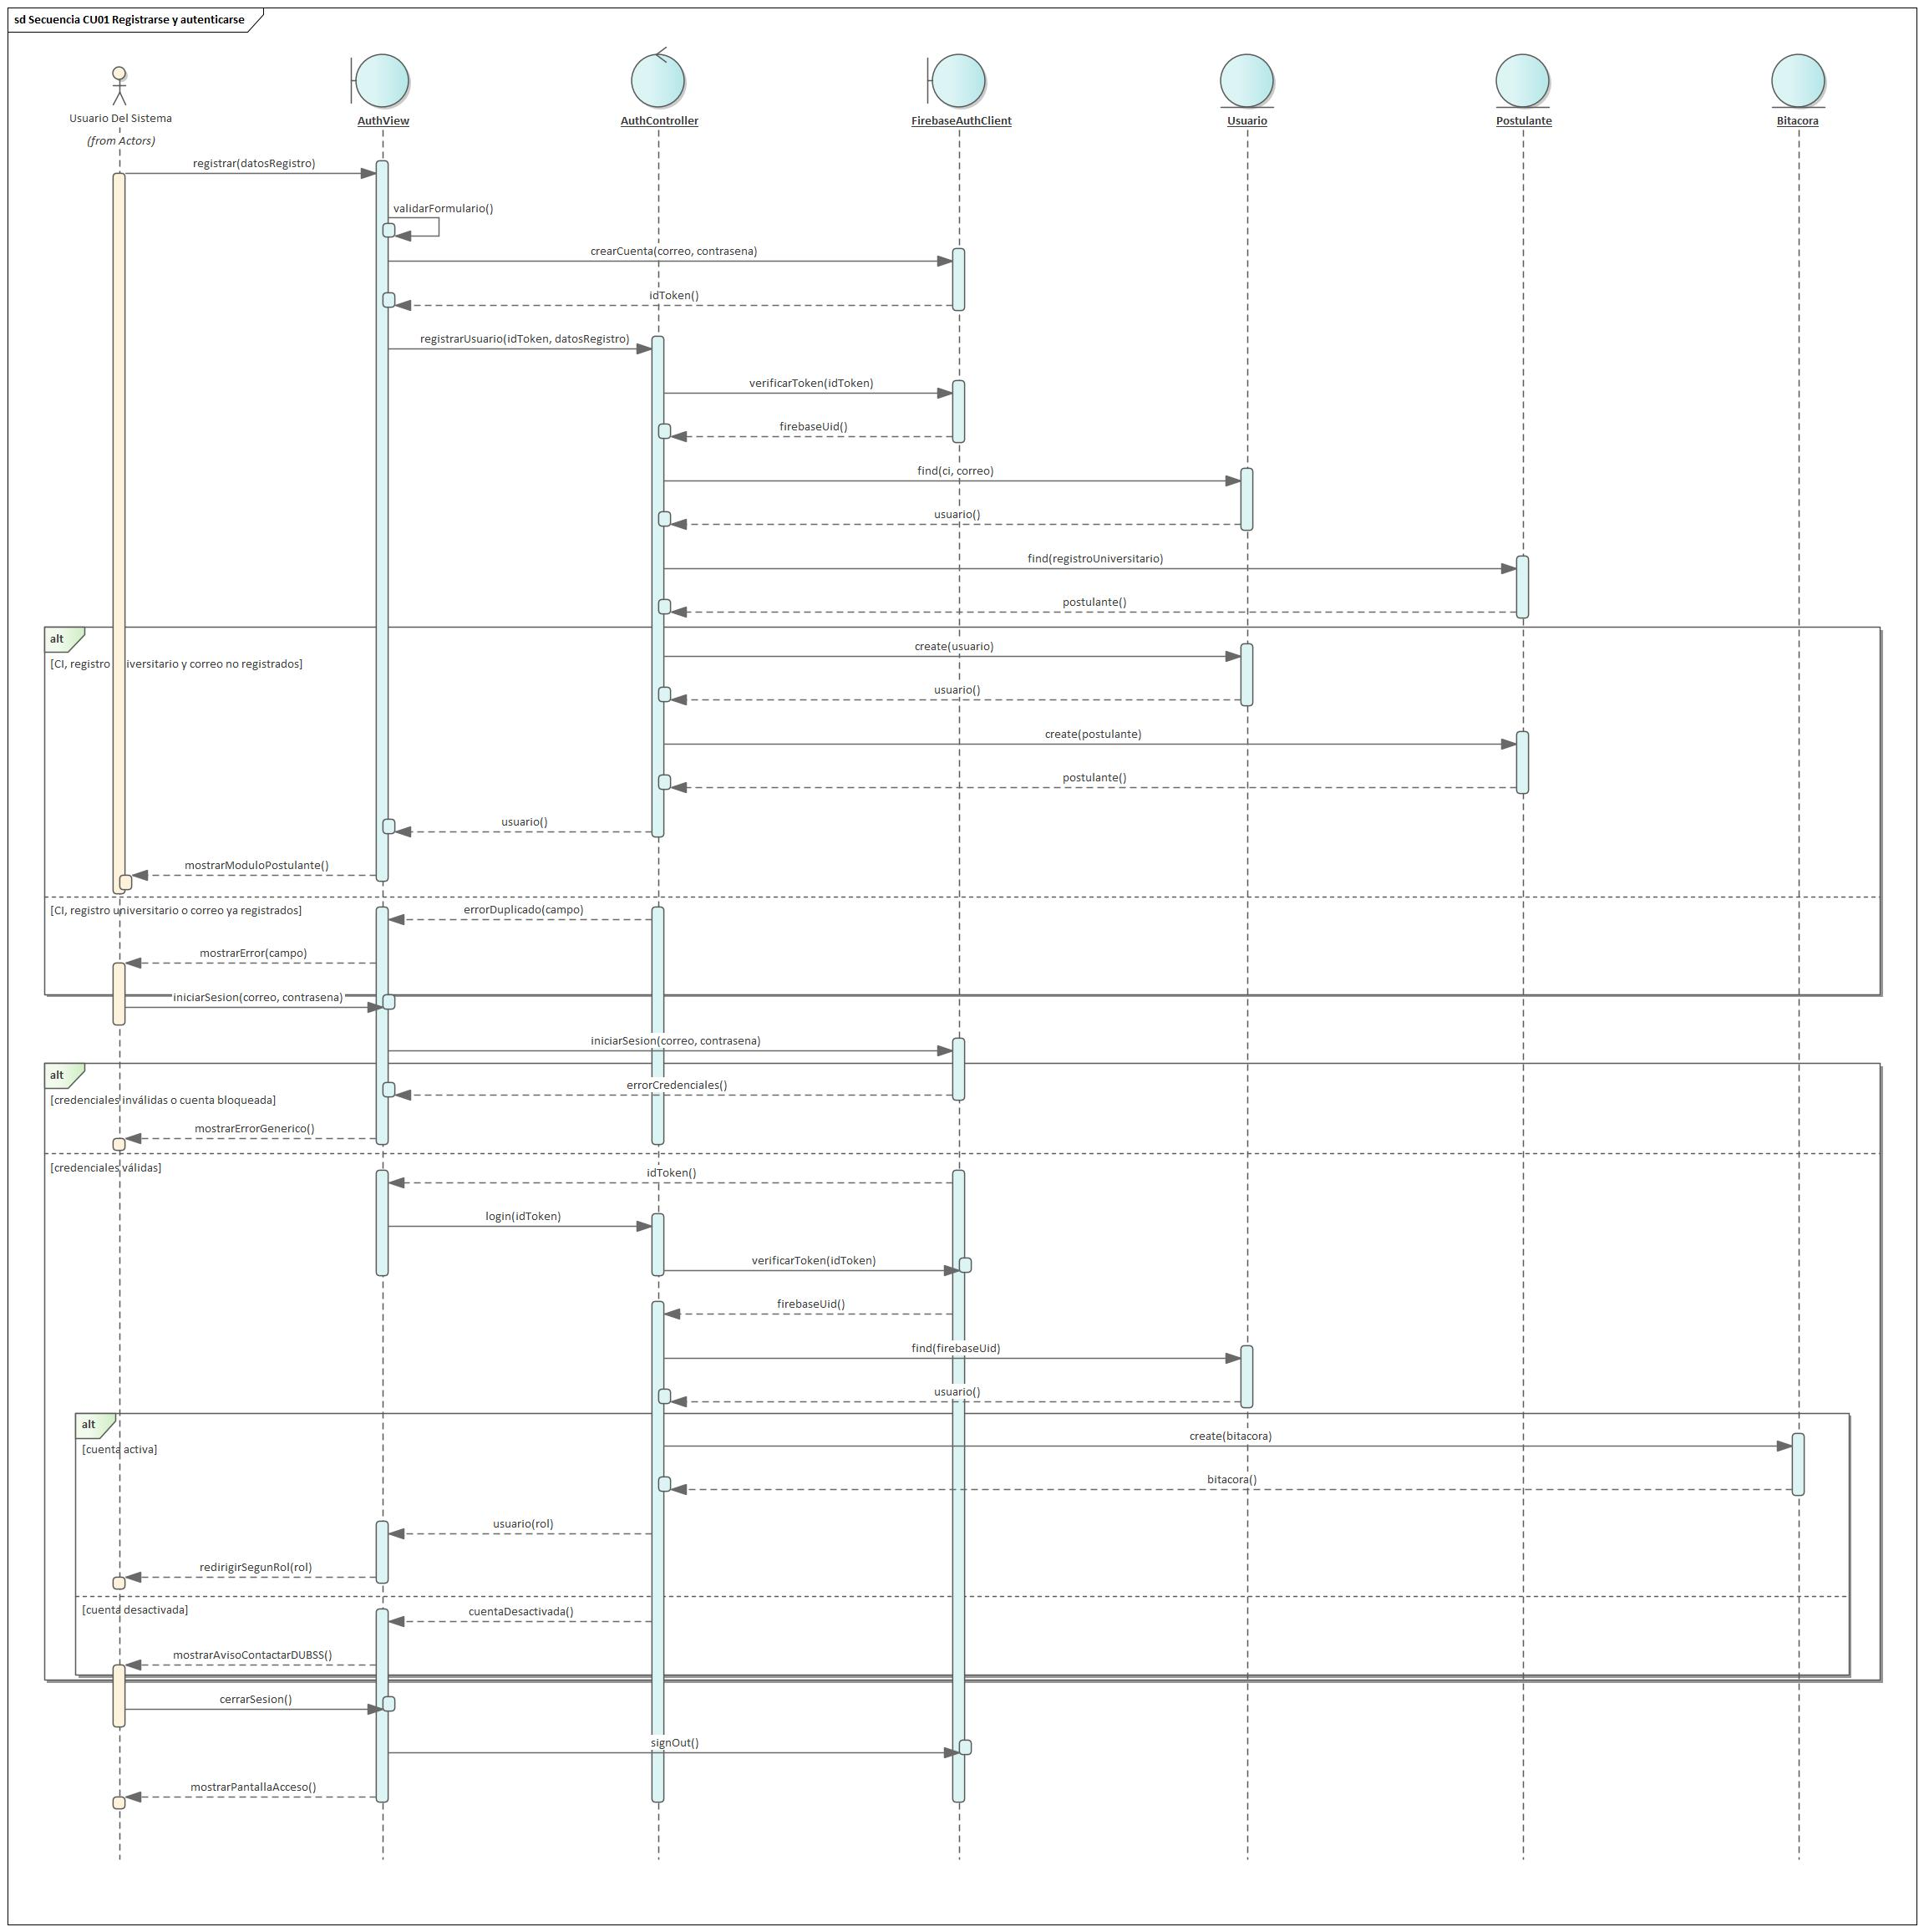
\includegraphics[width=\textwidth,height=0.75\textheight,keepaspectratio]{images/121_Secuencia_CU01_Registrarse_Autenticarse.jpg}

\smallskip
\noindent\raggedright\textit{Nota.} Elaboración propia.
\end{figure}

En el registro, el cliente envía los datos al backend; \textit{AuthController} comprueba que el CI, el registro universitario y el correo electrónico no existan, crea el \textit{Usuario} con el rol Postulante y la contraseña almacenada como hash, crea su perfil de \textit{Postulante} (con registro universitario y teléfono), abre la \textit{Sesion}, anota en la bitácora el registro y el inicio de sesión, y devuelve el token de acceso, el token de renovación y el usuario; si alguno de esos datos ya existe, informa el campo en conflicto y no crea la cuenta. En el inicio de sesión, el controlador busca al \textit{Usuario} por su correo electrónico; si las credenciales no son válidas o la cuenta está bloqueada, actualiza el contador de intentos fallidos y el bloqueo y responde con un mismo mensaje de error. Si son válidas y la cuenta está activa, abre la \textit{Sesion}, anota el acceso en la bitácora y devuelve los tokens y el usuario con su rol, según el cual se redirige al módulo correspondiente; si la cuenta está desactivada, niega el acceso e indica que debe comunicarse con la DUBSS. Cuando el token de acceso vence, el cliente solicita su renovación con el token de renovación: el controlador busca la \textit{Sesion} por el hash del token, la revoca y crea una nueva con un token de renovación nuevo; si la sesión no es válida, el usuario vuelve a la pantalla de acceso. Para cerrar sesión, el controlador revoca la \textit{Sesion} del dispositivo, sin afectar las de otros dispositivos. La contraseña (mínimo de 6 caracteres) se almacena solo como hash y el bloqueo tras 5 intentos fallidos consecutivos lo aplica el propio sistema.


\Needspace{0.9\textheight}
\subsubsection{7.4.2. Diseñar CU-02 Enviar postulación a Beca Comedor}\label{sec:cap7_disenar_cu02}

La Figura~\ref{fig:secuencia_cu02} presenta el diagrama de secuencia del CU-02.

\begin{figure}[H]
\caption{Diagrama de secuencia del CU-02 Enviar postulación a Beca Comedor}
\label{fig:secuencia_cu02}
\centering
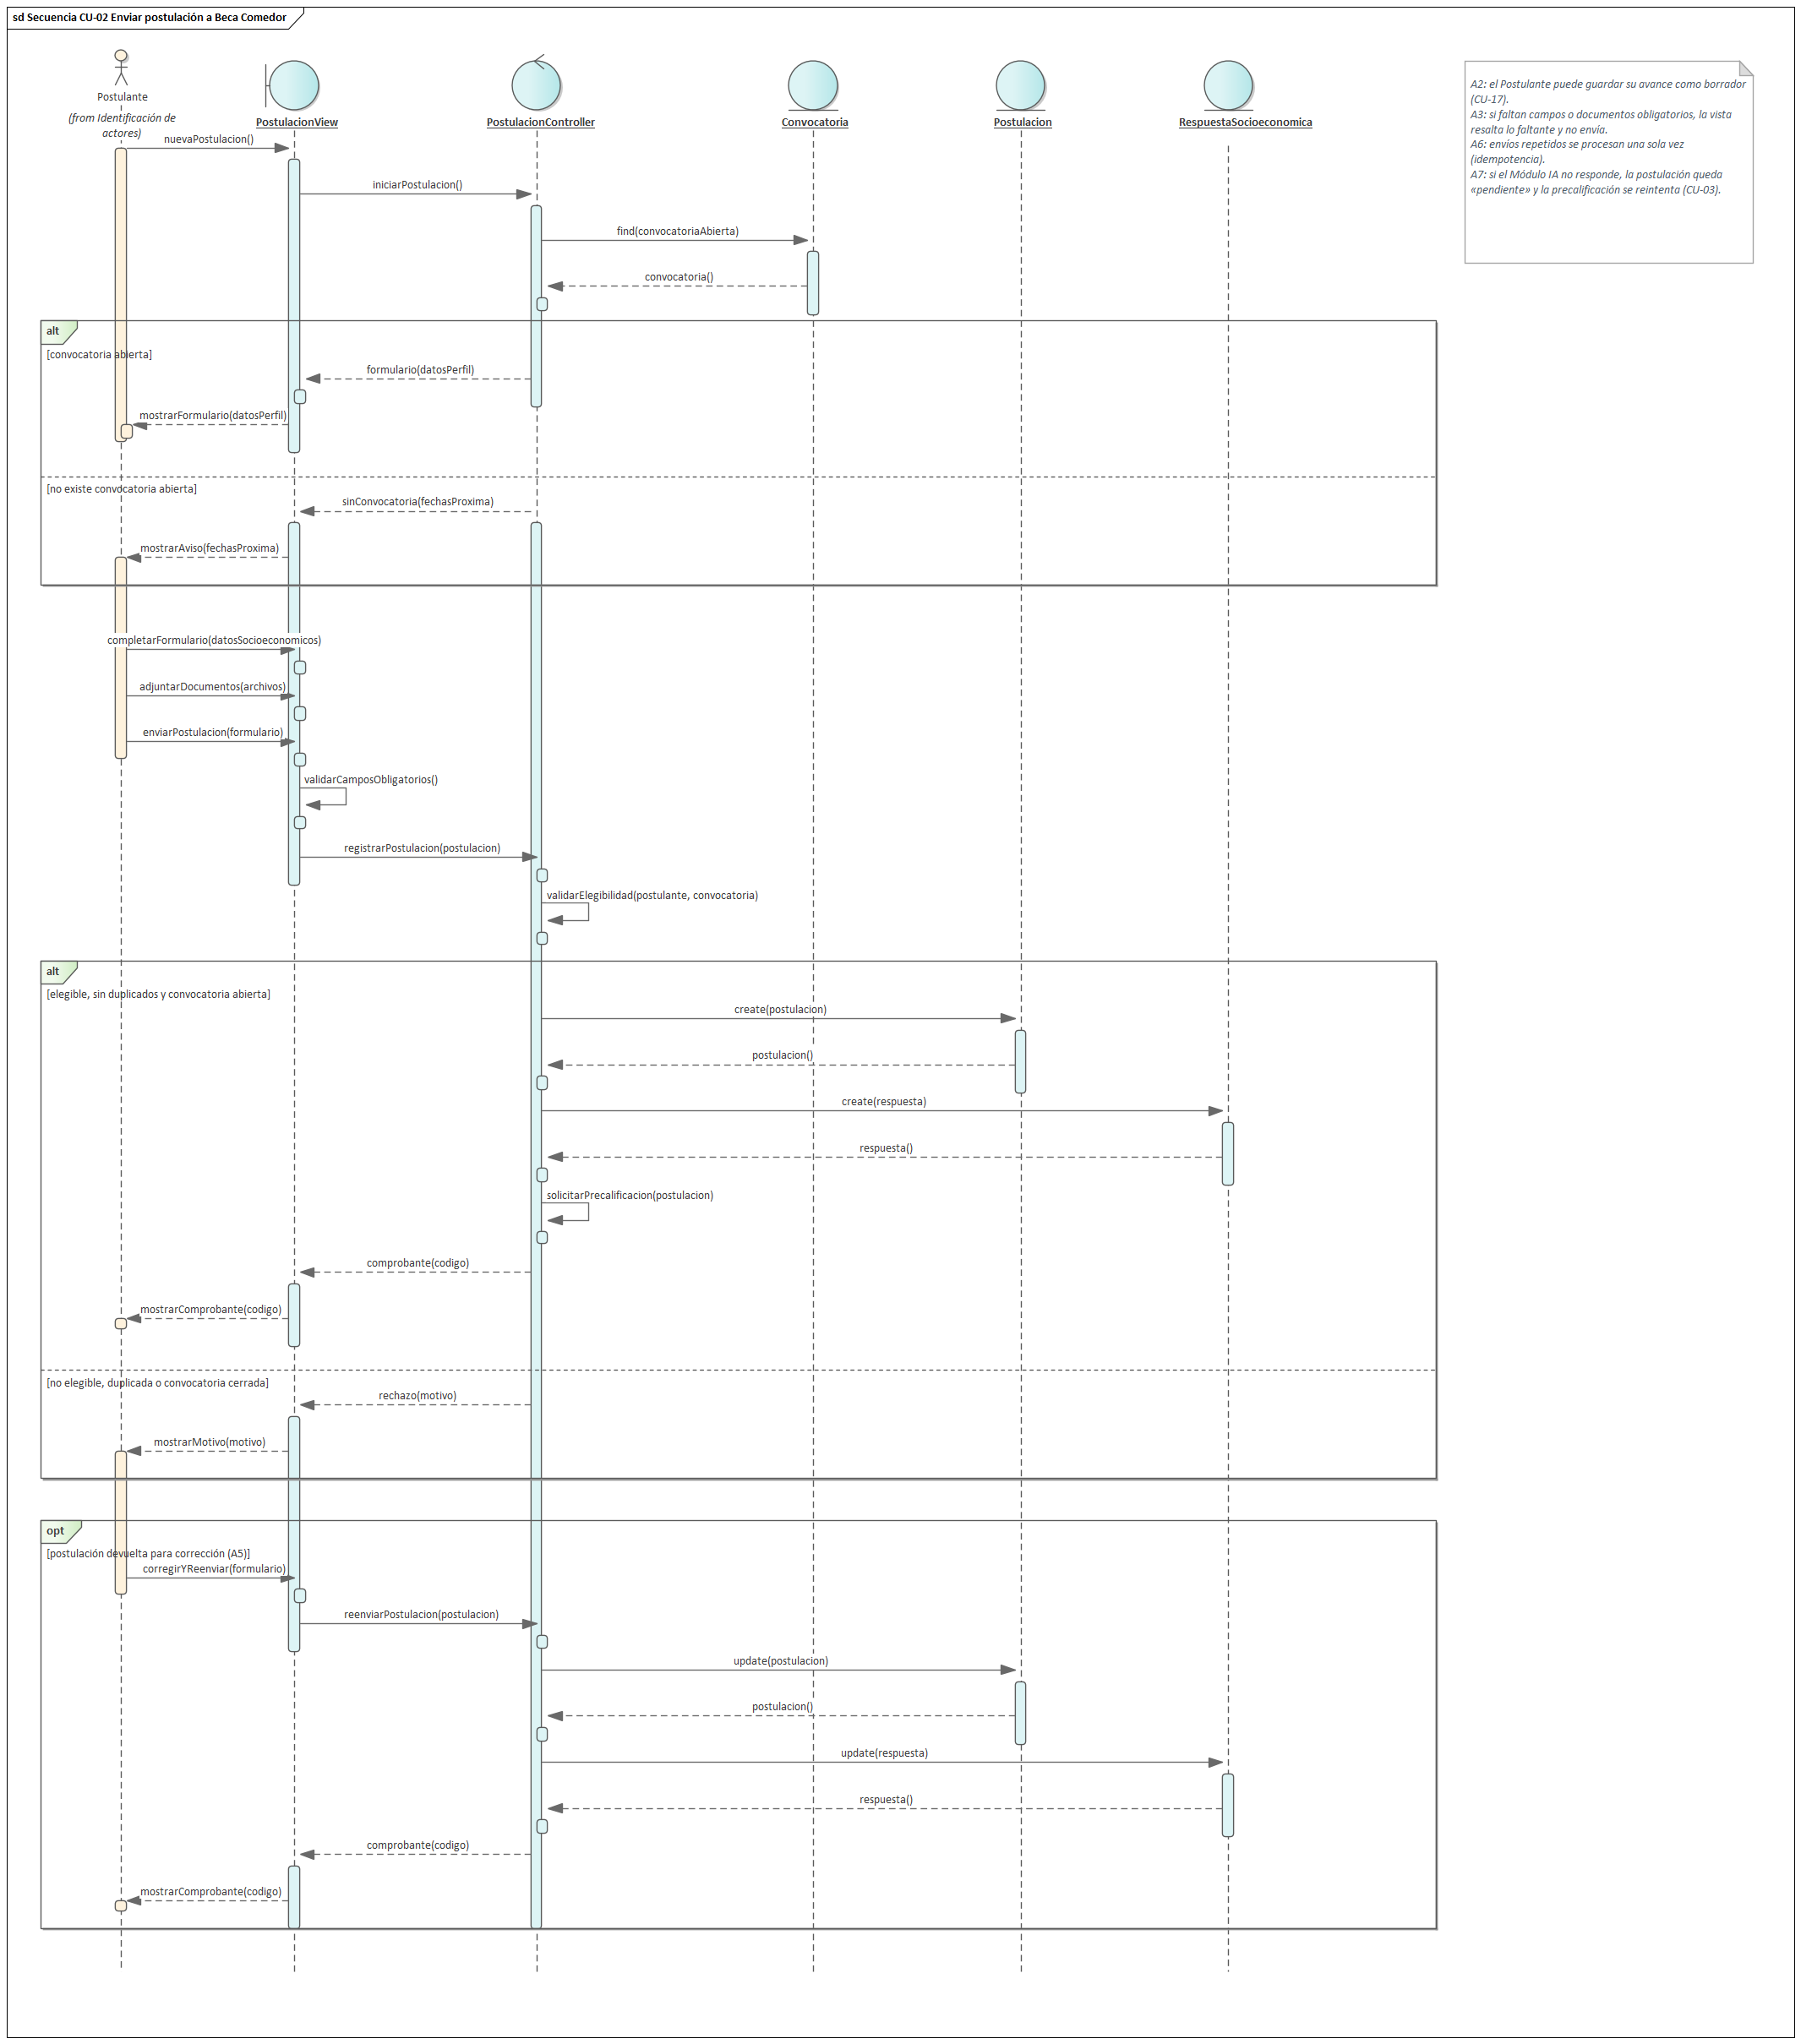
\includegraphics[width=\textwidth,height=0.75\textheight,keepaspectratio]{images/122_Secuencia_CU02_Enviar_Postulacion_Beca_Comedor.png}

\smallskip
\noindent\raggedright\textit{Nota.} Elaboración propia.
\end{figure}


\Needspace{0.9\textheight}
\subsubsection{7.4.3. Diseñar CU-03 Precalificar postulación con Inteligencia Artificial}\label{sec:cap7_disenar_cu03}

La Figura~\ref{fig:secuencia_cu03} presenta el diagrama de secuencia del CU-03.

\begin{figure}[H]
\caption{Diagrama de secuencia del CU-03 Precalificar postulación con Inteligencia Artificial}
\label{fig:secuencia_cu03}
\centering
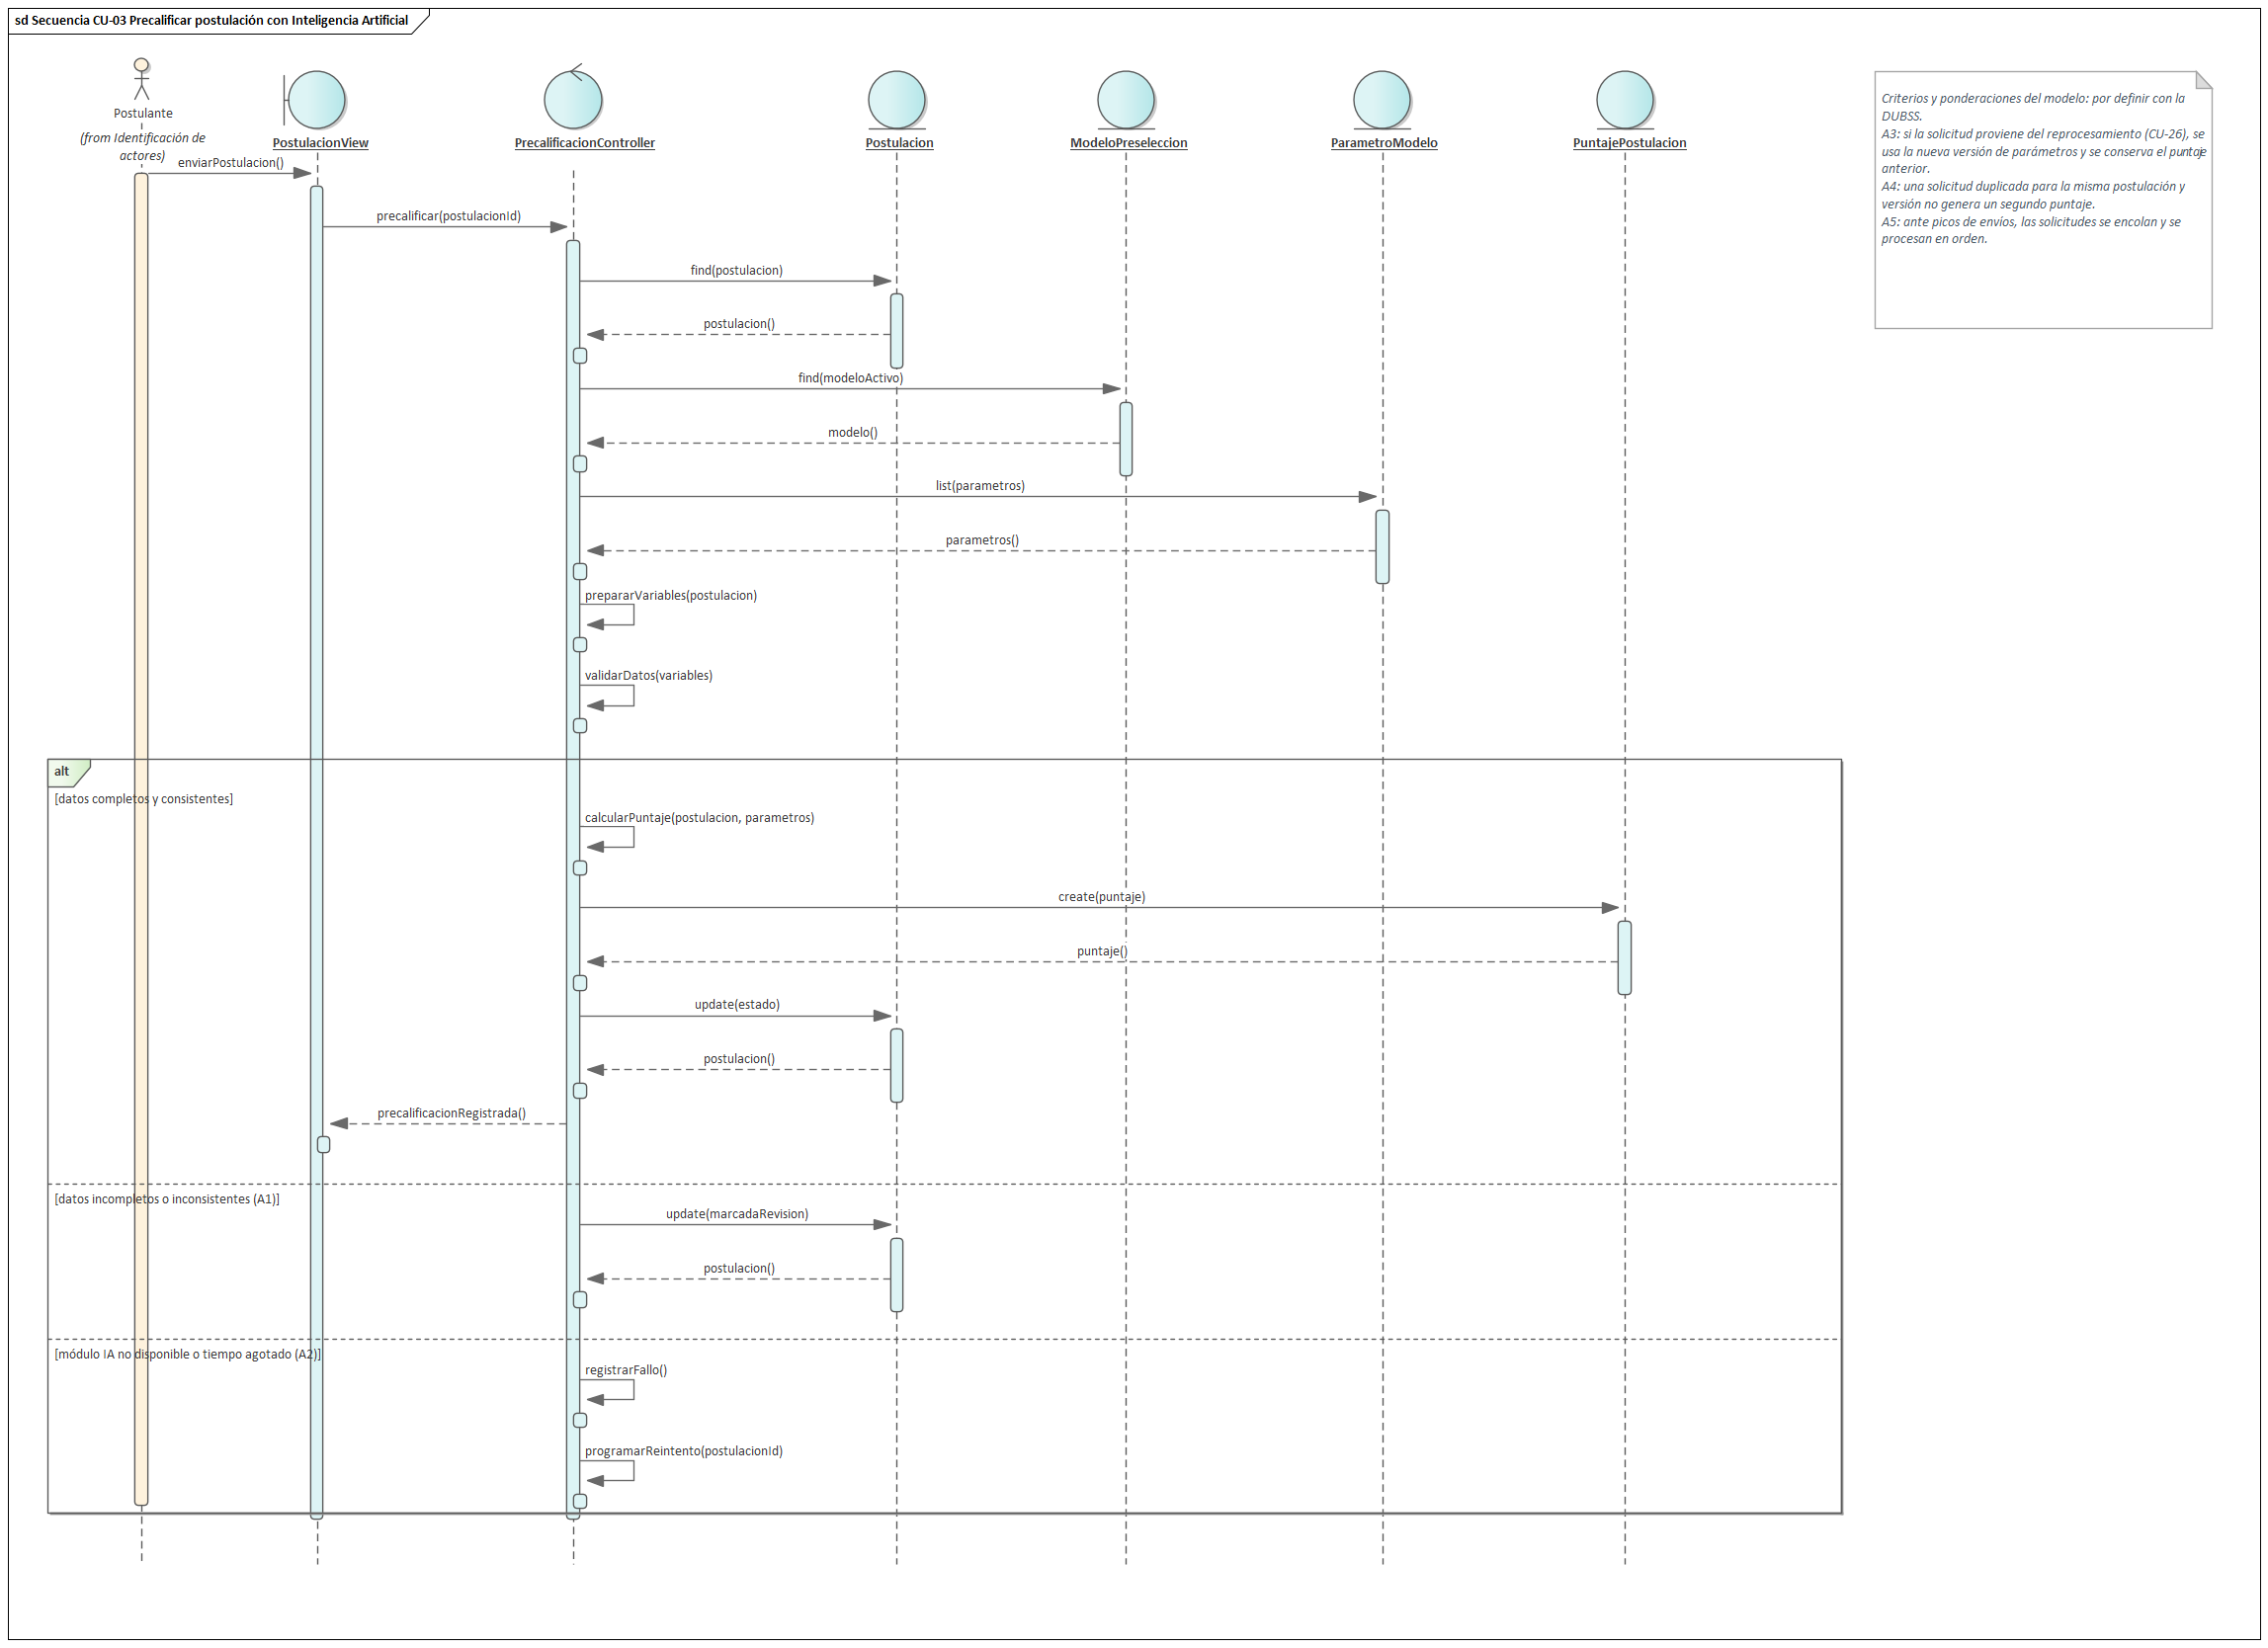
\includegraphics[width=\textwidth,height=0.75\textheight,keepaspectratio]{images/123_Secuencia_CU03_Precalificar_Postulacion_IA.png}

\smallskip
\noindent\raggedright\textit{Nota.} Elaboración propia.
\end{figure}


\Needspace{0.9\textheight}
\subsubsection{7.4.4. Diseñar CU-04 Consultar estado de postulación}\label{sec:cap7_disenar_cu04}

La Figura~\ref{fig:secuencia_cu04} presenta el diagrama de secuencia del CU-04.

\begin{figure}[H]
\caption{Diagrama de secuencia del CU-04 Consultar estado de postulación}
\label{fig:secuencia_cu04}
\centering
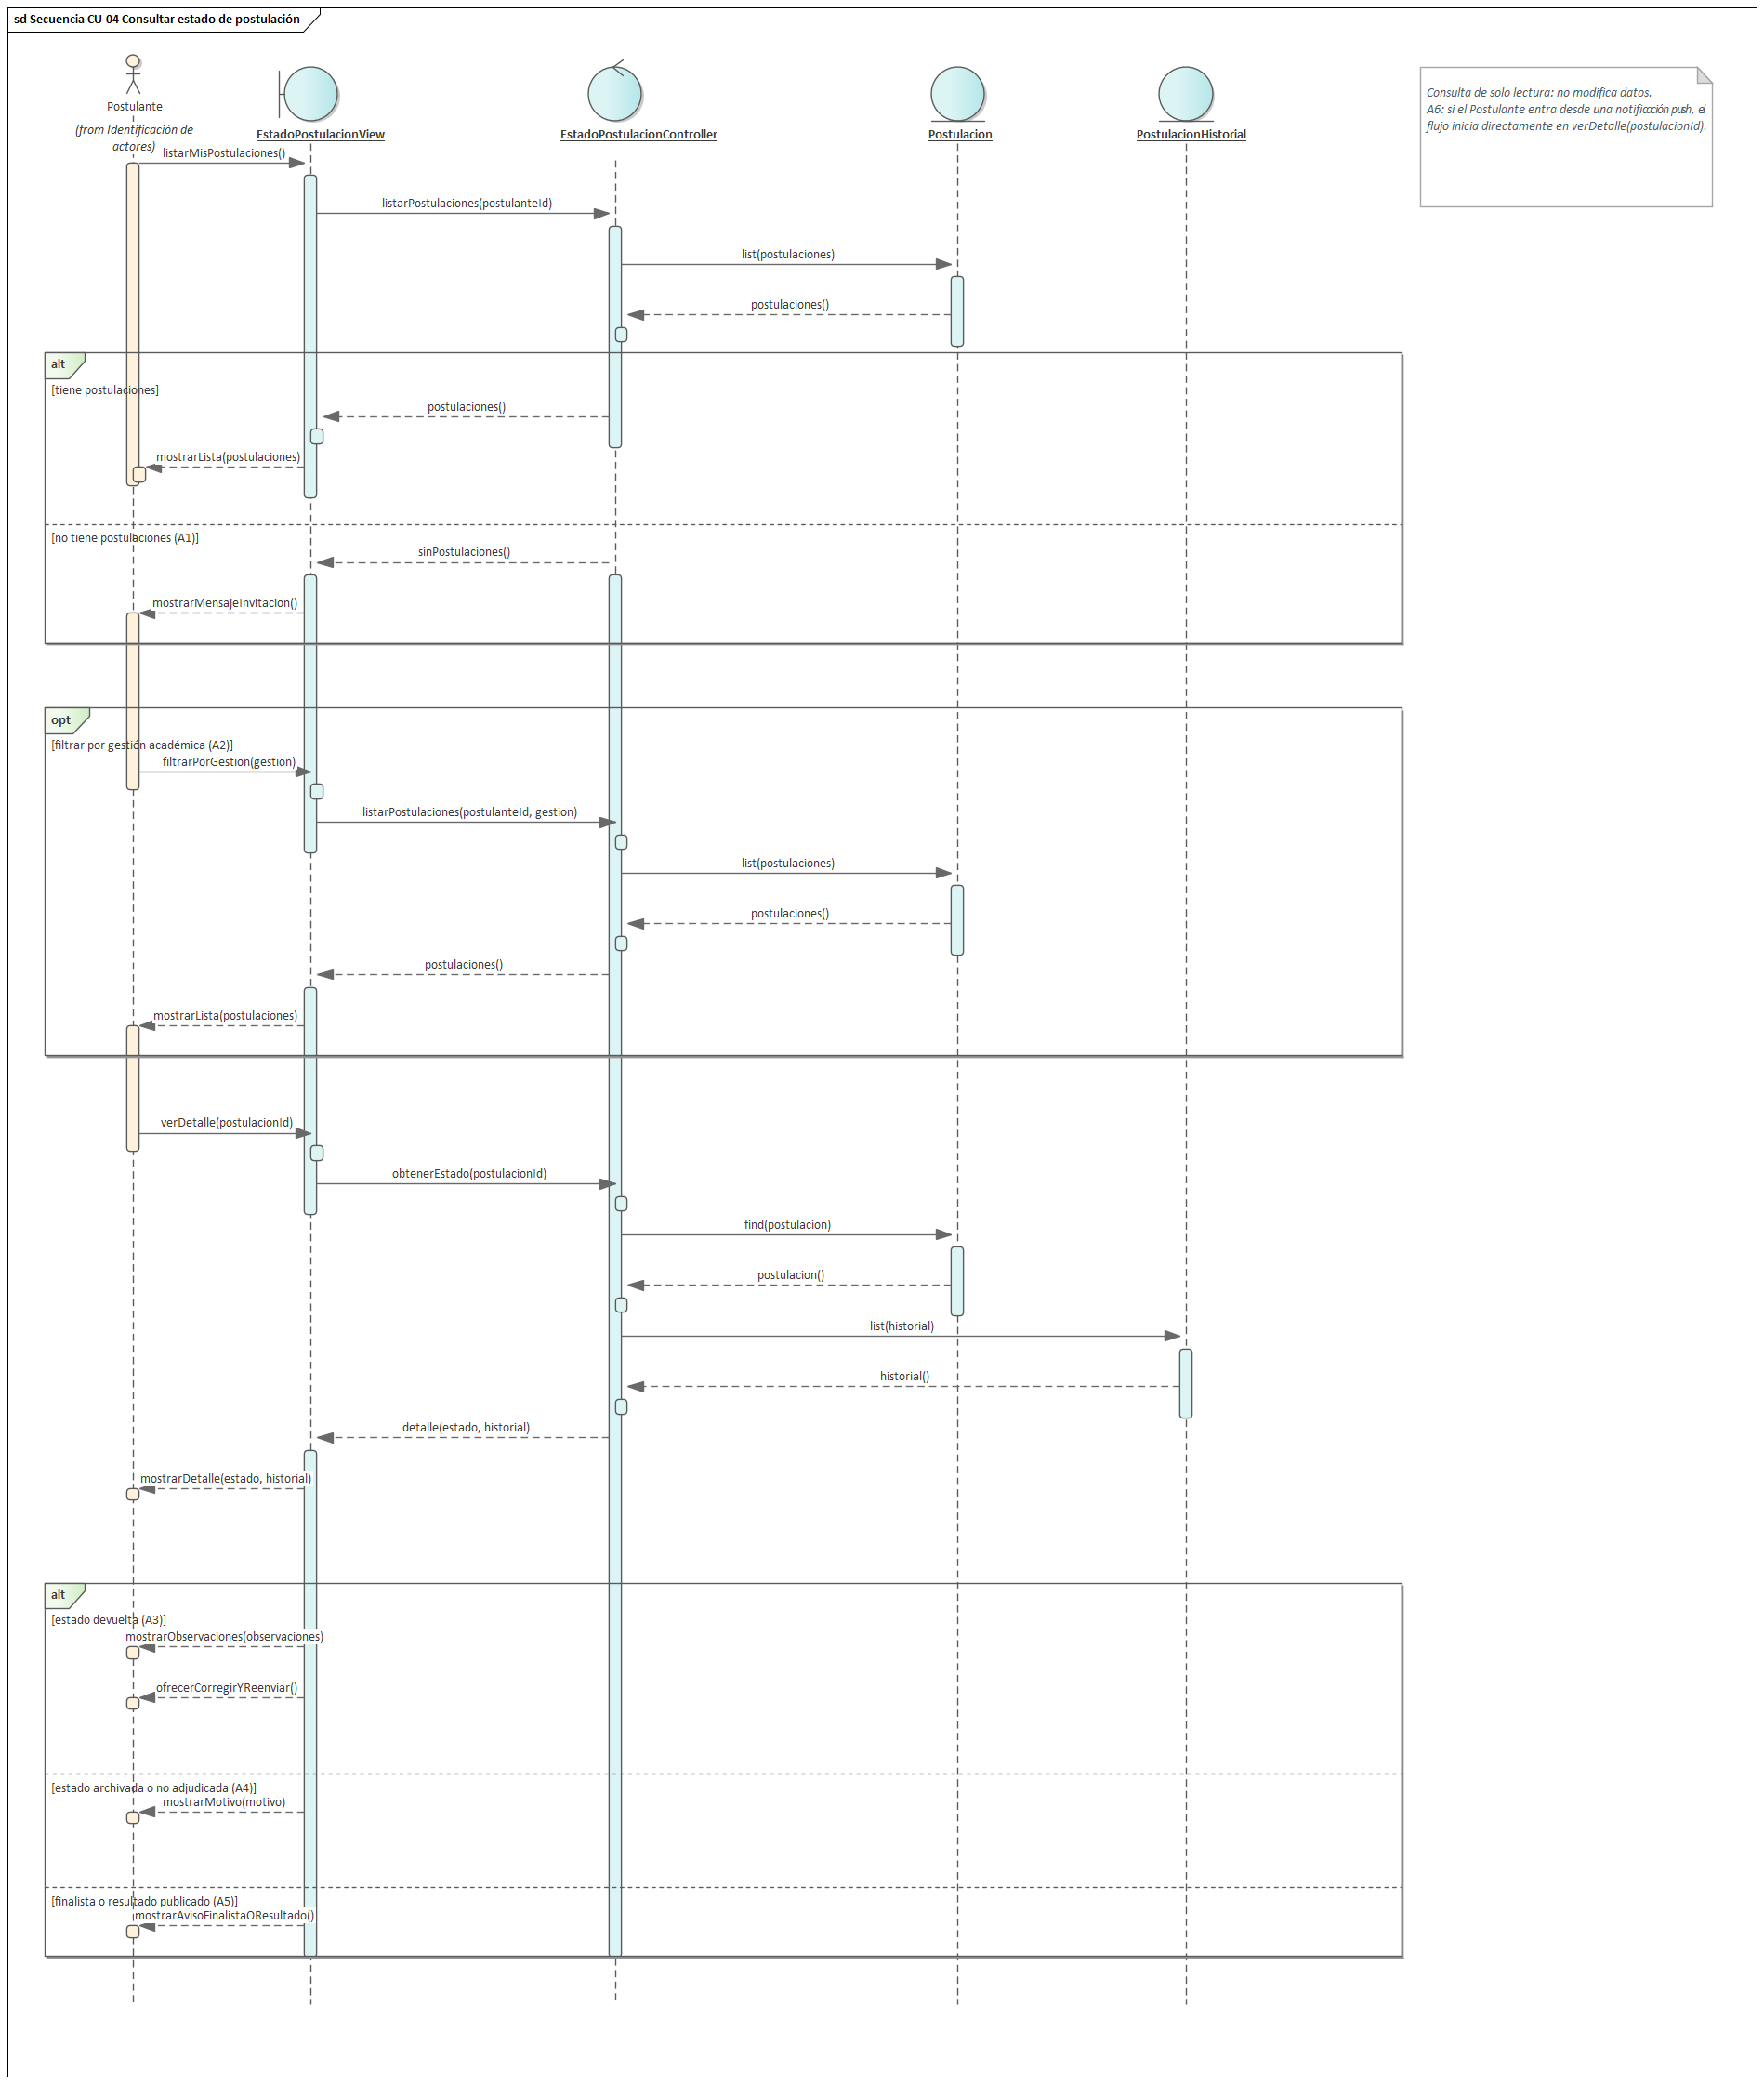
\includegraphics[width=\textwidth,height=0.75\textheight,keepaspectratio]{images/124_Secuencia_CU04_Consultar_Estado_Postulacion.png}

\smallskip
\noindent\raggedright\textit{Nota.} Elaboración propia.
\end{figure}


\Needspace{0.9\textheight}
\subsubsection{7.4.5. Diseñar CU-05 Auditar y adjudicar becas}\label{sec:cap7_disenar_cu05}

La Figura~\ref{fig:secuencia_cu05} presenta el diagrama de secuencia del CU-05.

\begin{figure}[H]
\caption{Diagrama de secuencia del CU-05 Auditar y adjudicar becas}
\label{fig:secuencia_cu05}
\centering
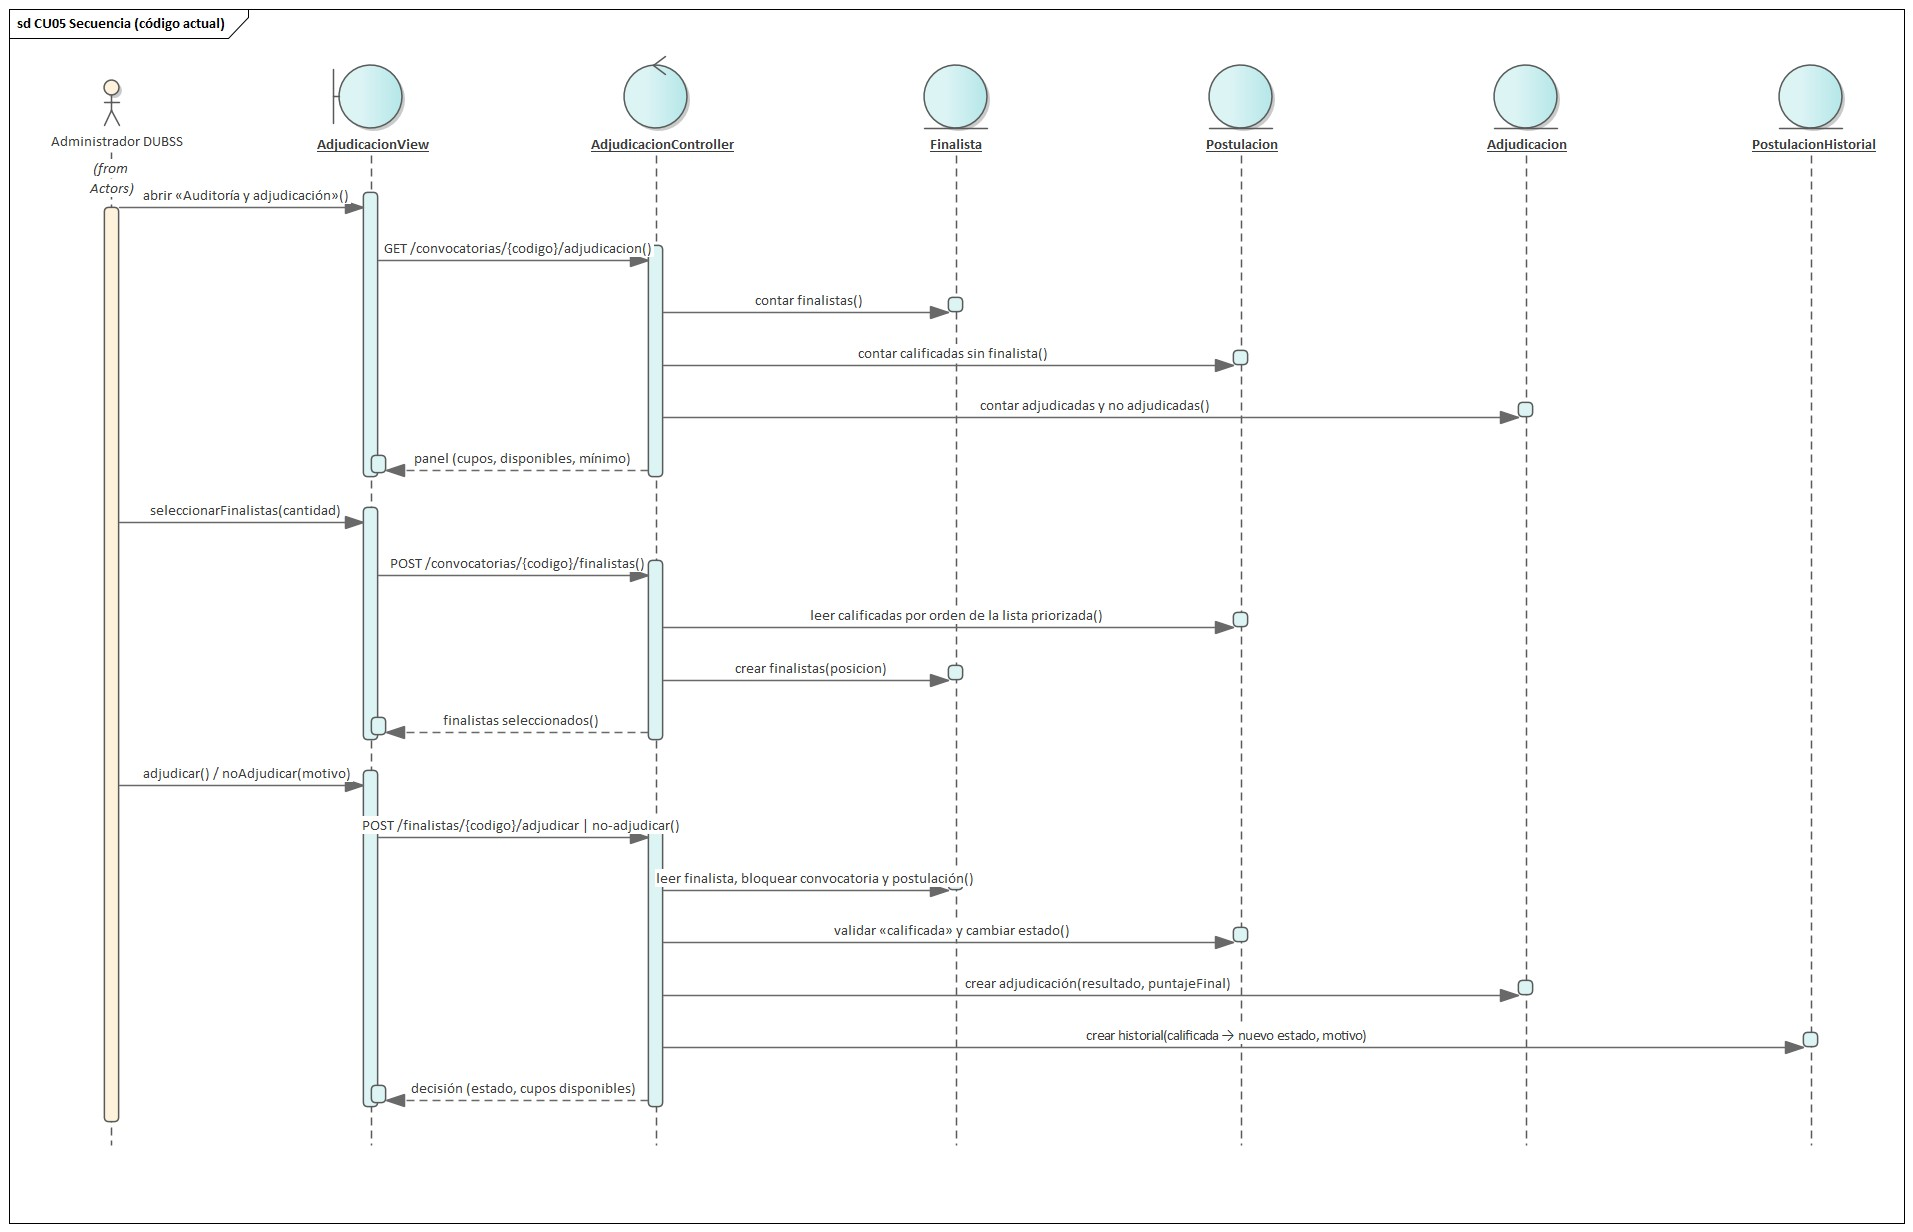
\includegraphics[width=\textwidth,height=0.75\textheight,keepaspectratio]{images/092_Secuencia_CU05_Auditar_Adjudicar_Becas.jpg}

\smallskip
\noindent\raggedright\textit{Nota.} Elaboración propia.
\end{figure}


\Needspace{0.9\textheight}
\subsubsection{7.4.6. Diseñar CU-06 Visualizar lista priorizada de postulantes}\label{sec:cap7_disenar_cu06}

La Figura~\ref{fig:secuencia_cu06} presenta el diagrama de secuencia del CU-06.

\begin{figure}[H]
\caption{Diagrama de secuencia del CU-06 Visualizar lista priorizada de postulantes}
\label{fig:secuencia_cu06}
\centering
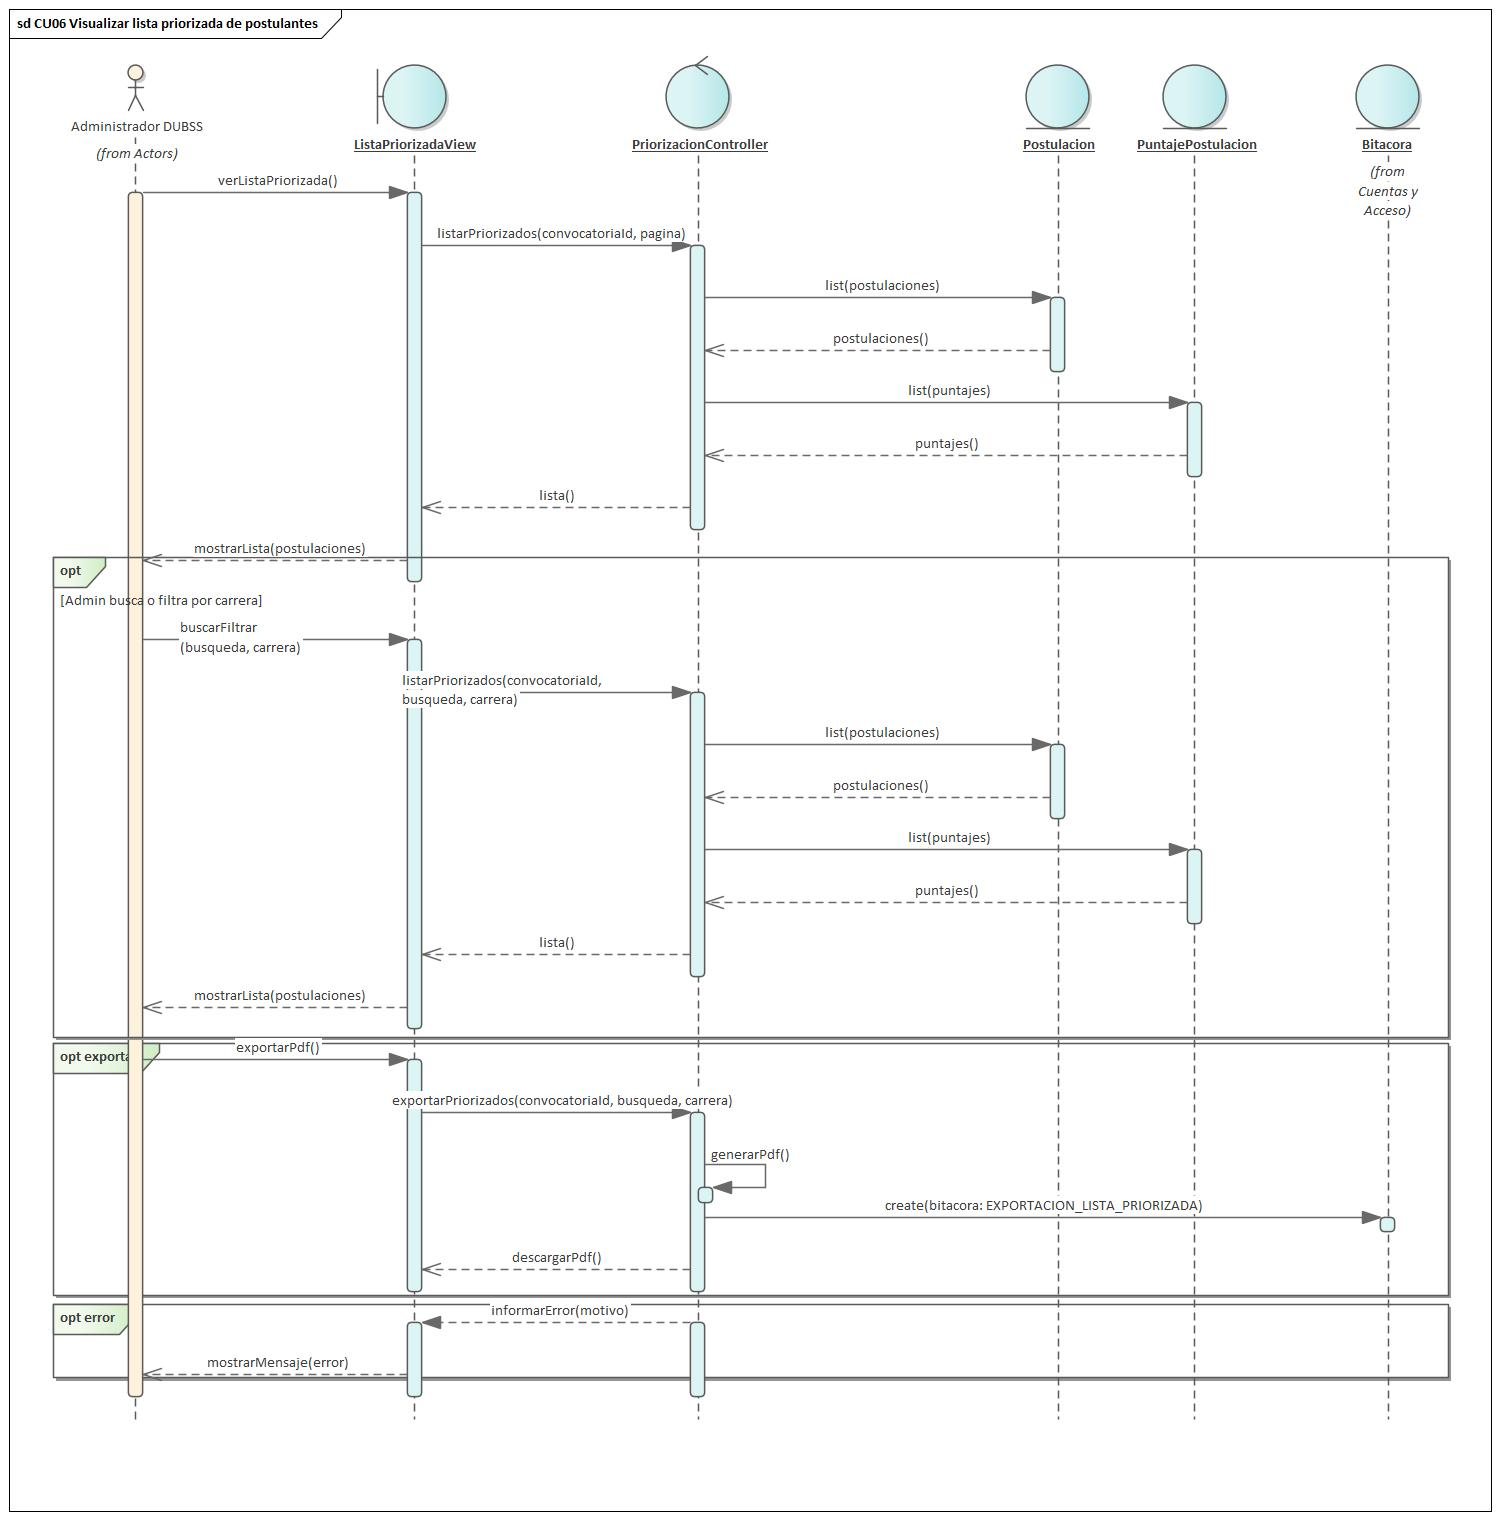
\includegraphics[width=\textwidth,height=0.75\textheight,keepaspectratio]{images/093_Secuencia_CU06_Visualizar_Lista_Priorizada_Postulantes.jpg}

\smallskip
\noindent\raggedright\textit{Nota.} Elaboración propia.
\end{figure}


\Needspace{0.9\textheight}
\subsubsection{7.4.7. Diseñar CU-07 Auditar expediente finalista}\label{sec:cap7_disenar_cu07}

La Figura~\ref{fig:secuencia_cu07} presenta el diagrama de secuencia del CU-07.

\begin{figure}[H]
\caption{Diagrama de secuencia del CU-07 Auditar expediente finalista}
\label{fig:secuencia_cu07}
\centering
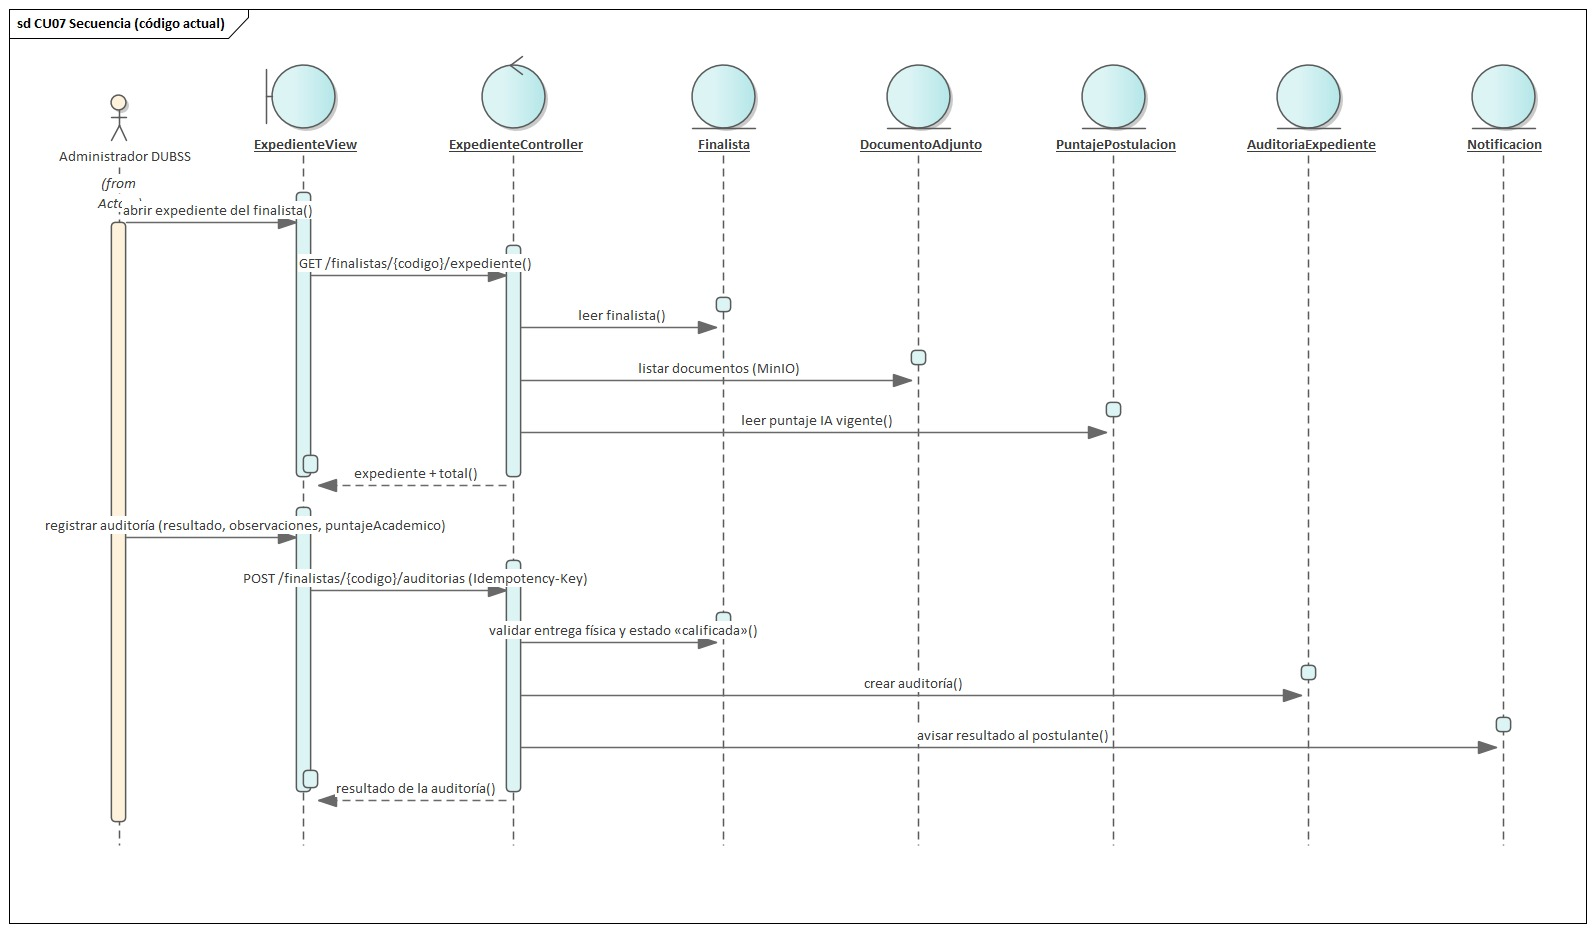
\includegraphics[width=\textwidth,height=0.75\textheight,keepaspectratio]{images/094_Secuencia_CU07_Auditar_Expediente_Finalista.jpg}

\smallskip
\noindent\raggedright\textit{Nota.} Elaboración propia.
\end{figure}


\Needspace{0.9\textheight}
\subsubsection{7.4.8. Diseñar CU-08 Generar acta de adjudicación}\label{sec:cap7_disenar_cu08}

La Figura~\ref{fig:secuencia_cu08} presenta el diagrama de secuencia del CU-08.

\begin{figure}[H]
\caption{Diagrama de secuencia del CU-08 Generar acta de adjudicación}
\label{fig:secuencia_cu08}
\centering
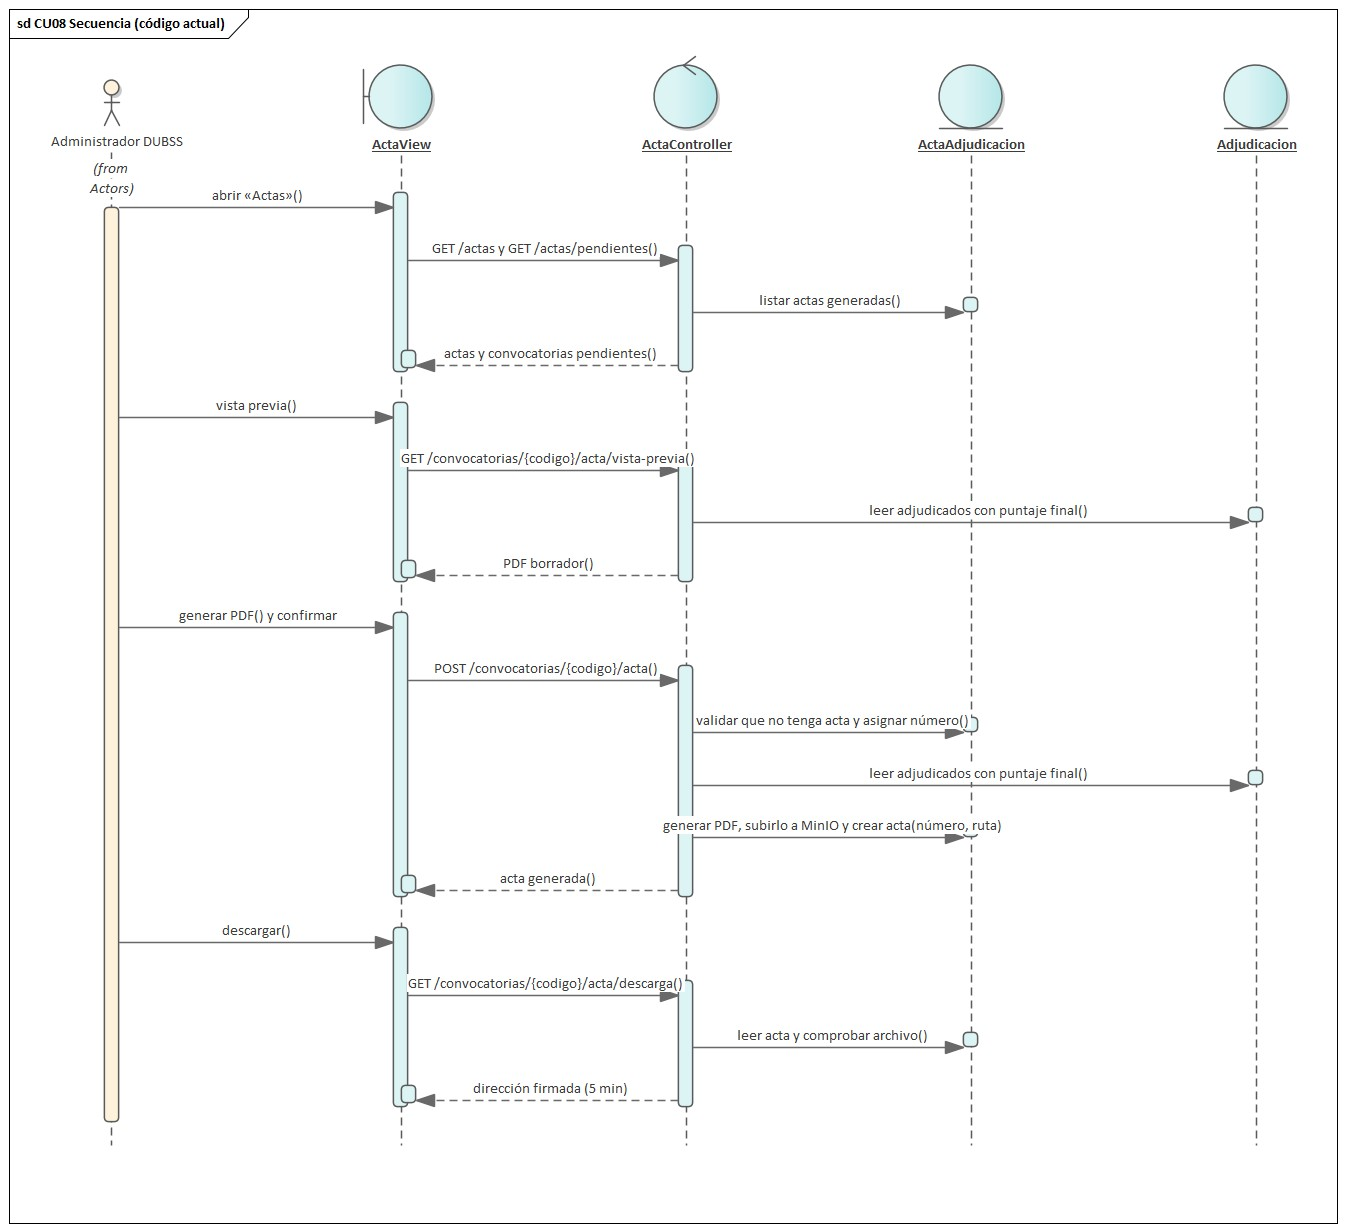
\includegraphics[width=\textwidth,height=0.75\textheight,keepaspectratio]{images/095_Secuencia_CU08_Generar_Acta_Adjudicacion.jpg}

\smallskip
\noindent\raggedright\textit{Nota.} Elaboración propia.
\end{figure}


\Needspace{0.9\textheight}
\subsubsection{7.4.9. Diseñar CU-09 Generar planilla de asistencia}\label{sec:cap7_disenar_cu09}

La Figura~\ref{fig:secuencia_cu09} presenta el diagrama de secuencia del CU-09.

\begin{figure}[H]
\caption{Diagrama de secuencia del CU-09 Generar planilla de asistencia}
\label{fig:secuencia_cu09}
\centering
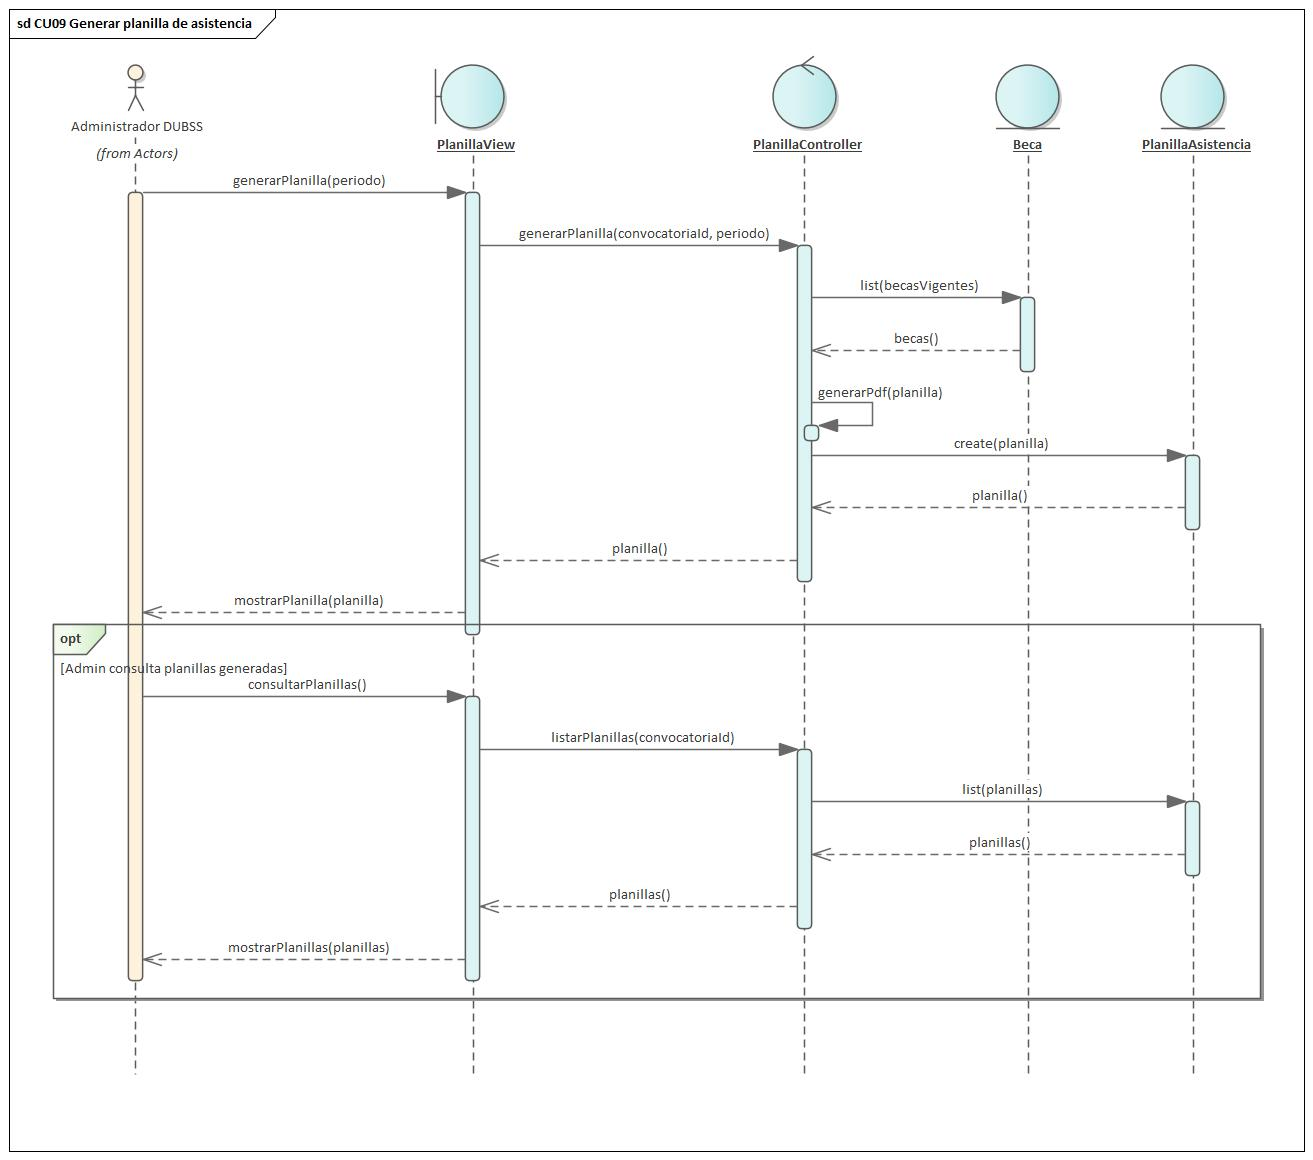
\includegraphics[width=\textwidth,height=0.75\textheight,keepaspectratio]{images/096_Secuencia_CU09_Generar_Planilla_Asistencia.jpg}

\smallskip
\noindent\raggedright\textit{Nota.} Elaboración propia.
\end{figure}


\Needspace{0.9\textheight}
\subsubsection{7.4.10. Diseñar CU-10 Registrar asistencia digital}\label{sec:cap7_disenar_cu10}

La Figura~\ref{fig:secuencia_cu10} presenta el diagrama de secuencia del CU-10.

\begin{figure}[H]
\caption{Diagrama de secuencia del CU-10 Registrar asistencia digital}
\label{fig:secuencia_cu10}
\centering
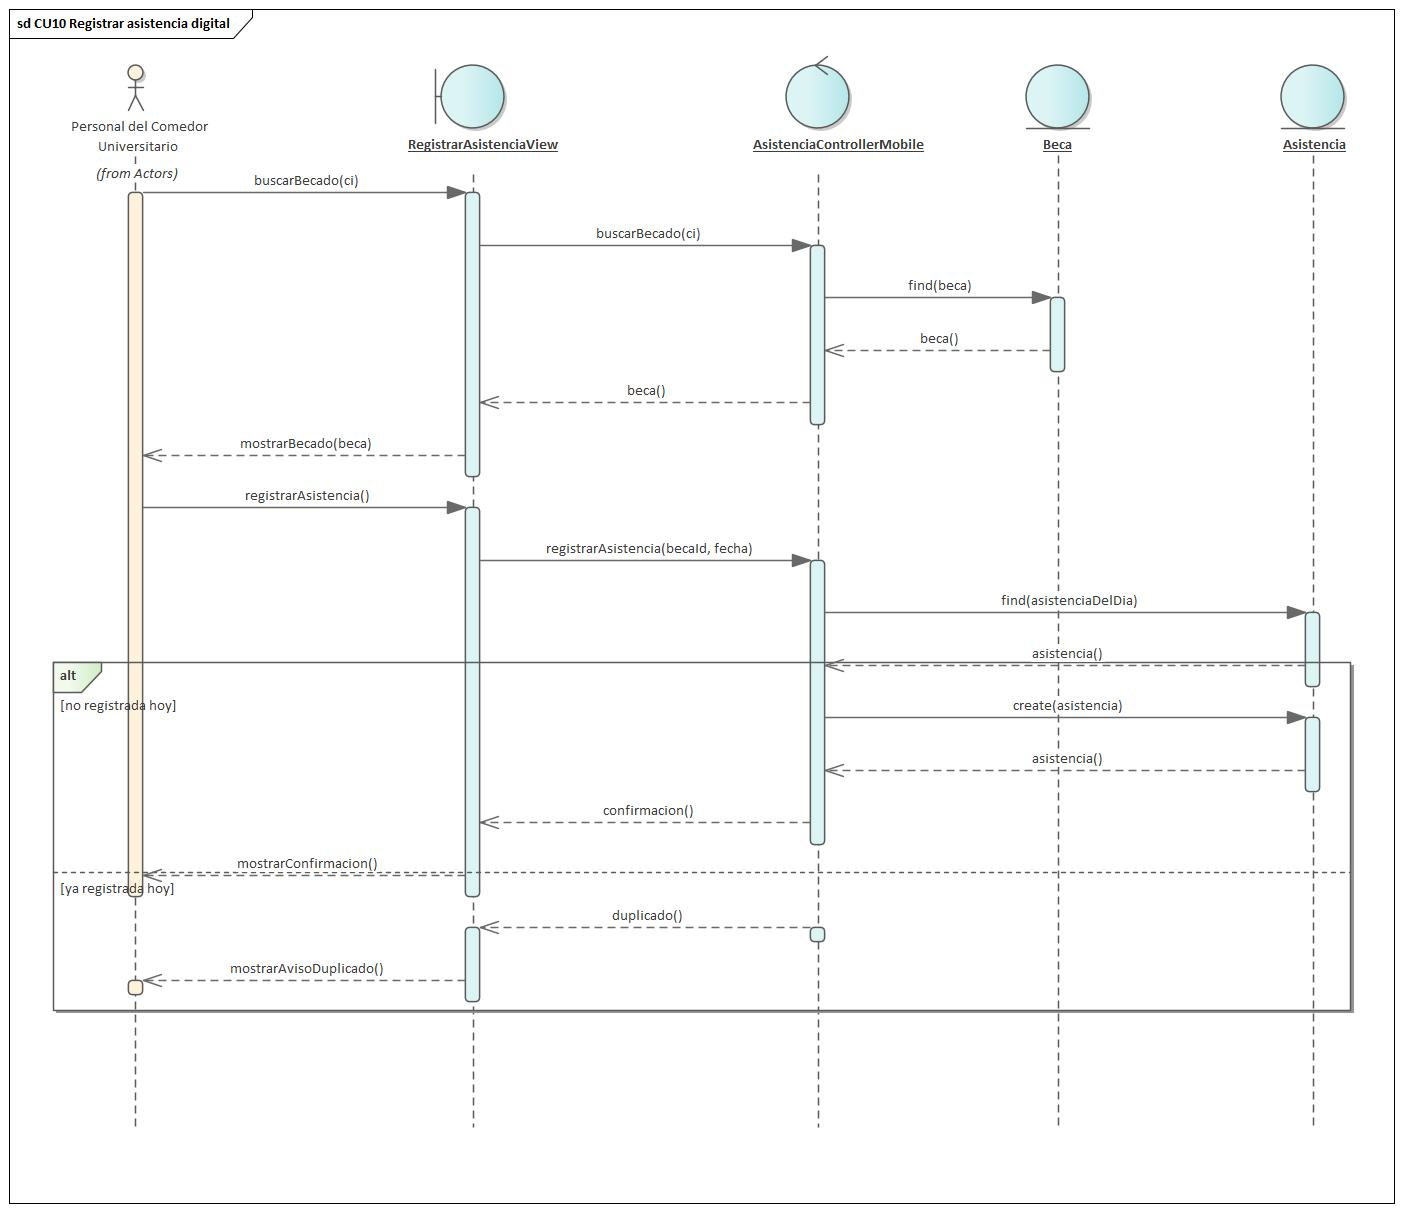
\includegraphics[width=\textwidth,height=0.75\textheight,keepaspectratio]{images/097_Secuencia_CU10_Registrar_Asistencia_Digital.jpg}

\smallskip
\noindent\raggedright\textit{Nota.} Elaboración propia.
\end{figure}


\Needspace{0.9\textheight}
\subsubsection{7.4.11. Diseñar CU-11 Cotejar registro contra respaldo físico}\label{sec:cap7_disenar_cu11}

La Figura~\ref{fig:secuencia_cu11} presenta el diagrama de secuencia del CU-11.

\begin{figure}[H]
\caption{Diagrama de secuencia del CU-11 Cotejar registro contra respaldo físico}
\label{fig:secuencia_cu11}
\centering
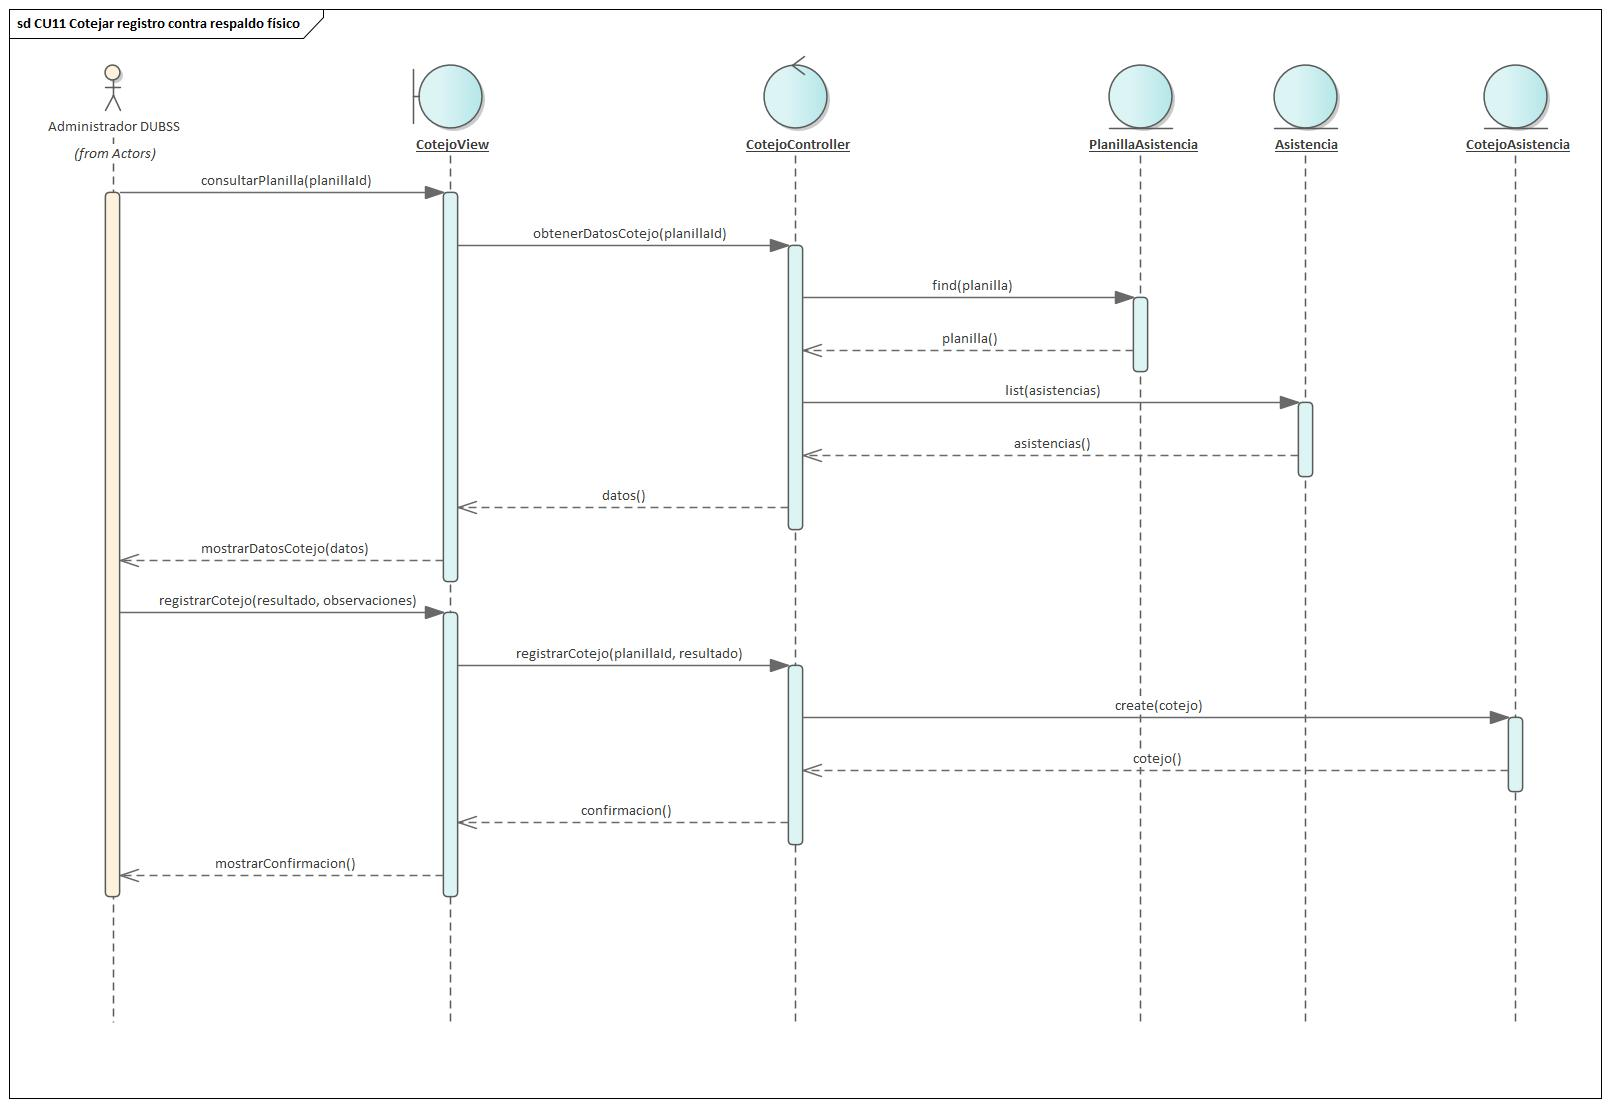
\includegraphics[width=\textwidth,height=0.75\textheight,keepaspectratio]{images/098_Secuencia_CU11_Cotejar_Registro_Respaldo_Fisico.jpg}

\smallskip
\noindent\raggedright\textit{Nota.} Elaboración propia.
\end{figure}


\Needspace{0.9\textheight}
\subsubsection{7.4.12. Diseñar CU-12 Visualizar dashboard de indicadores BI}\label{sec:cap7_disenar_cu12}

La Figura~\ref{fig:secuencia_cu12} presenta el diagrama de secuencia del CU-12.

\begin{figure}[H]
\caption{Diagrama de secuencia del CU-12 Visualizar dashboard de indicadores BI}
\label{fig:secuencia_cu12}
\centering
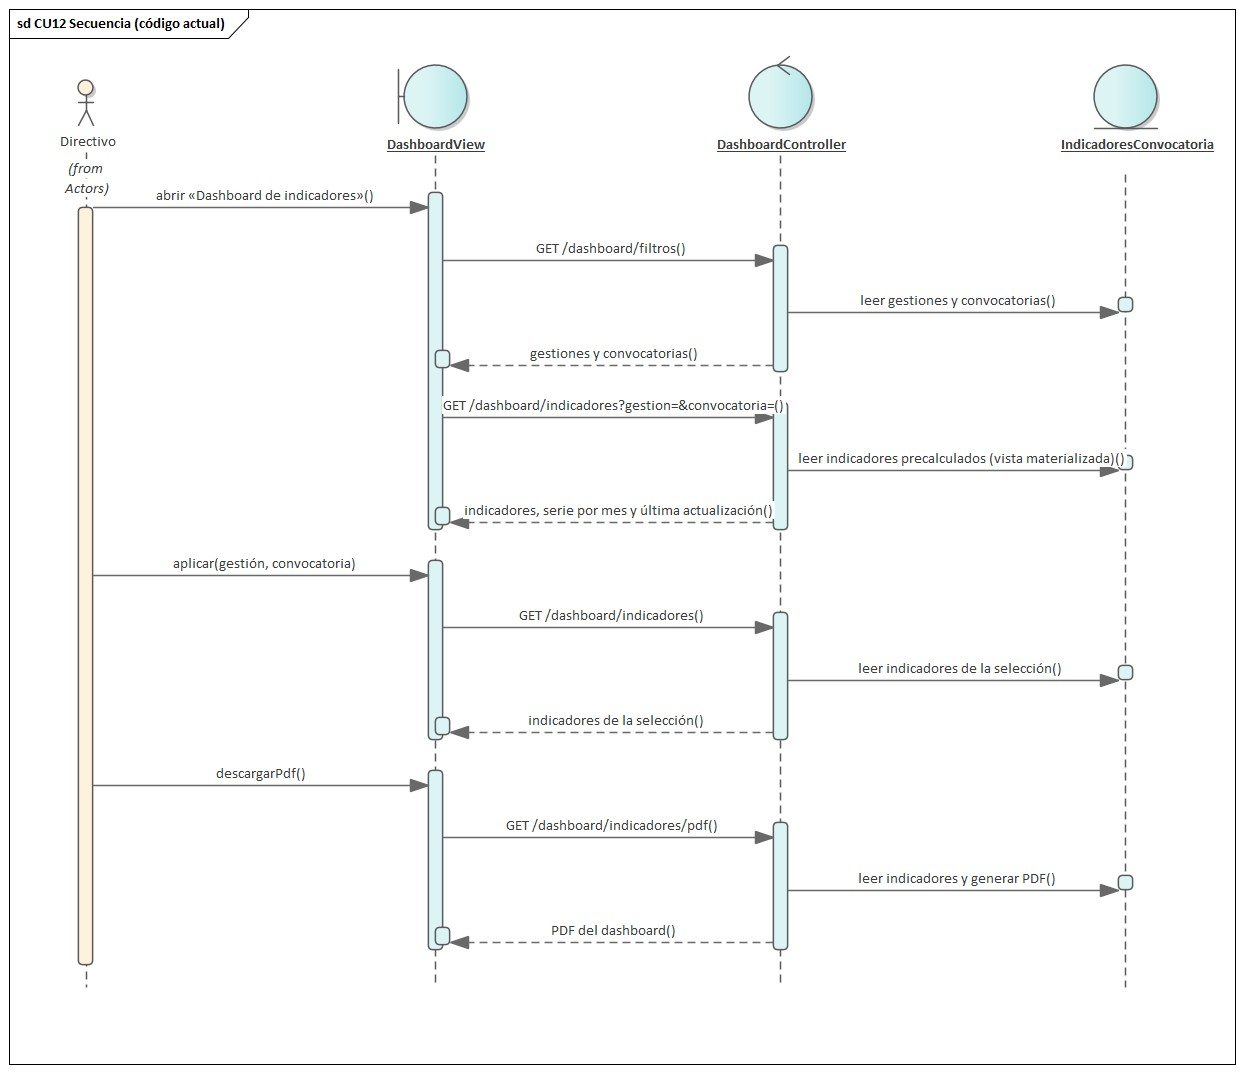
\includegraphics[width=\textwidth,height=0.75\textheight,keepaspectratio]{images/099_Secuencia_CU12_Visualizar_Dashboard_Indicadores_BI.jpg}

\smallskip
\noindent\raggedright\textit{Nota.} Elaboración propia.
\end{figure}


\Needspace{0.9\textheight}
\subsubsection{7.4.13. Diseñar CU-13 Gestionar convocatoria y gestión académica}\label{sec:cap7_disenar_cu13}

La Figura~\ref{fig:secuencia_cu13} presenta el diagrama de secuencia del CU-13.

\begin{figure}[H]
\caption{Diagrama de secuencia del CU-13 Gestionar convocatoria y gestión académica}
\label{fig:secuencia_cu13}
\centering
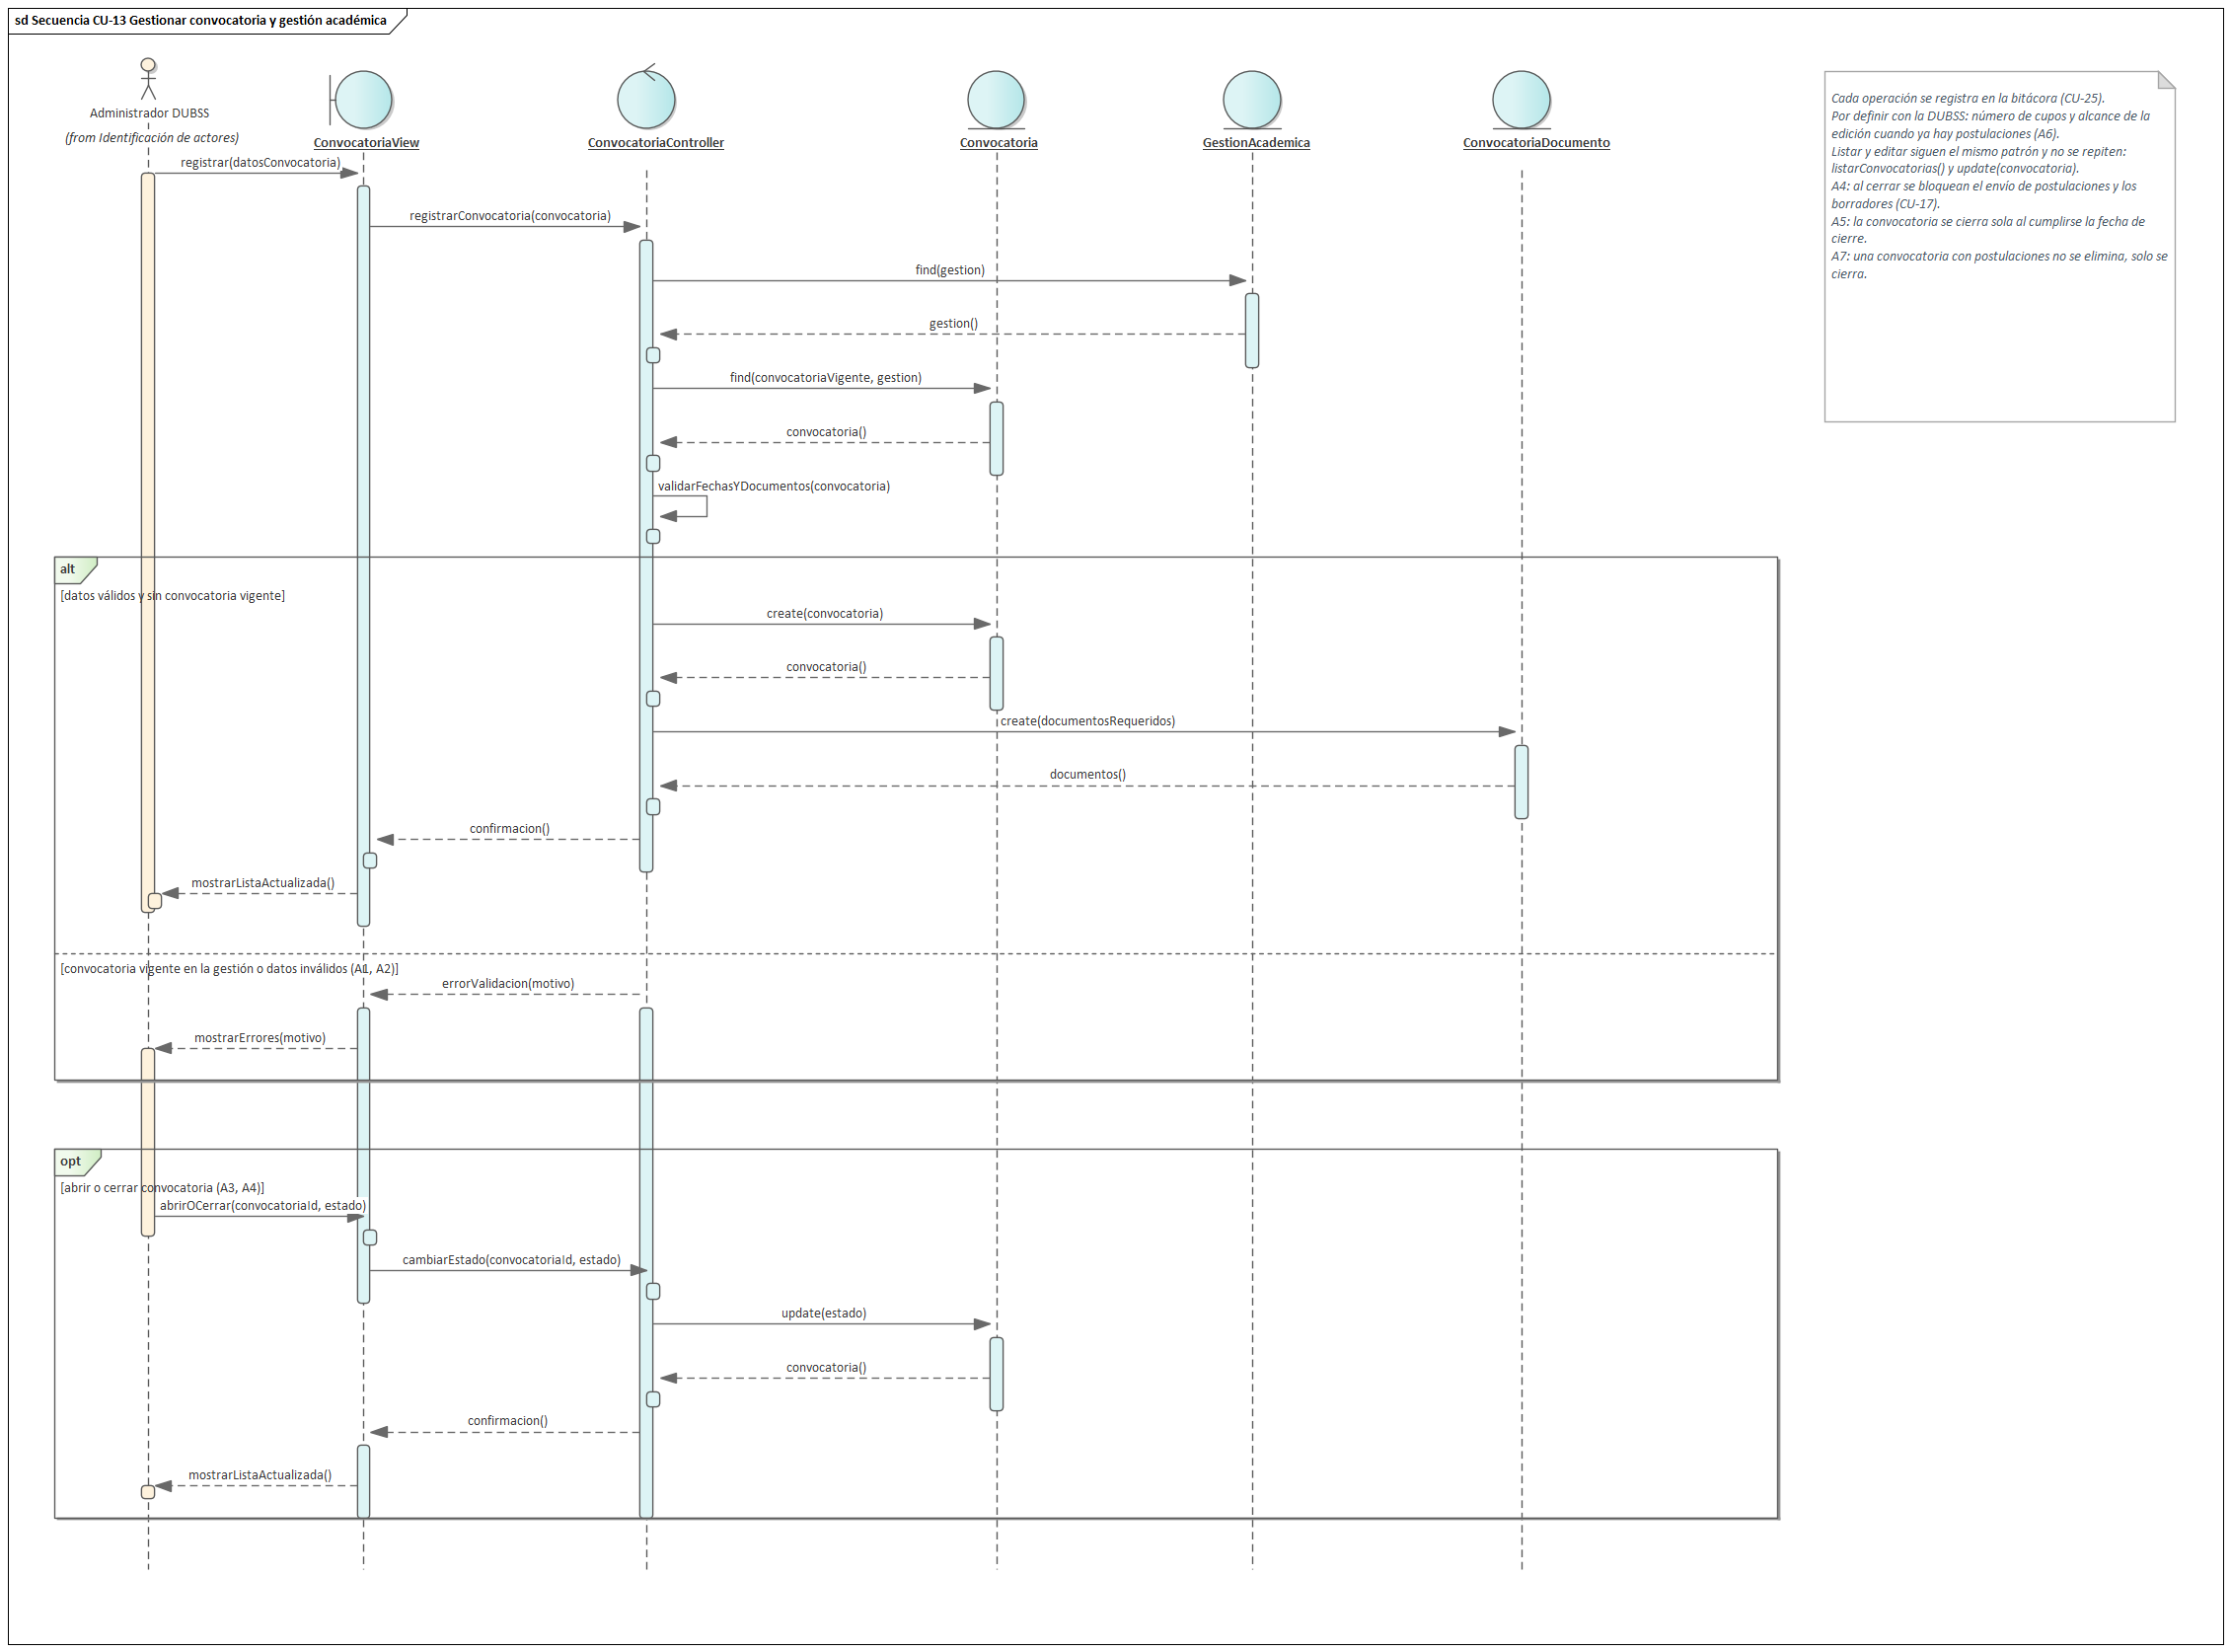
\includegraphics[width=\textwidth,height=0.75\textheight,keepaspectratio]{images/125_Secuencia_CU13_Gestionar_Convocatoria_Gestion_Academica.png}

\smallskip
\noindent\raggedright\textit{Nota.} Elaboración propia.
\end{figure}


\Needspace{0.9\textheight}
\subsubsection{7.4.14. Diseñar CU-14 Gestionar usuarios y roles}\label{sec:cap7_disenar_cu14}

La Figura~\ref{fig:secuencia_cu14} presenta el diagrama de secuencia del CU-14.

\begin{figure}[H]
\caption{Diagrama de secuencia del CU-14 Gestionar usuarios y roles}
\label{fig:secuencia_cu14}
\centering
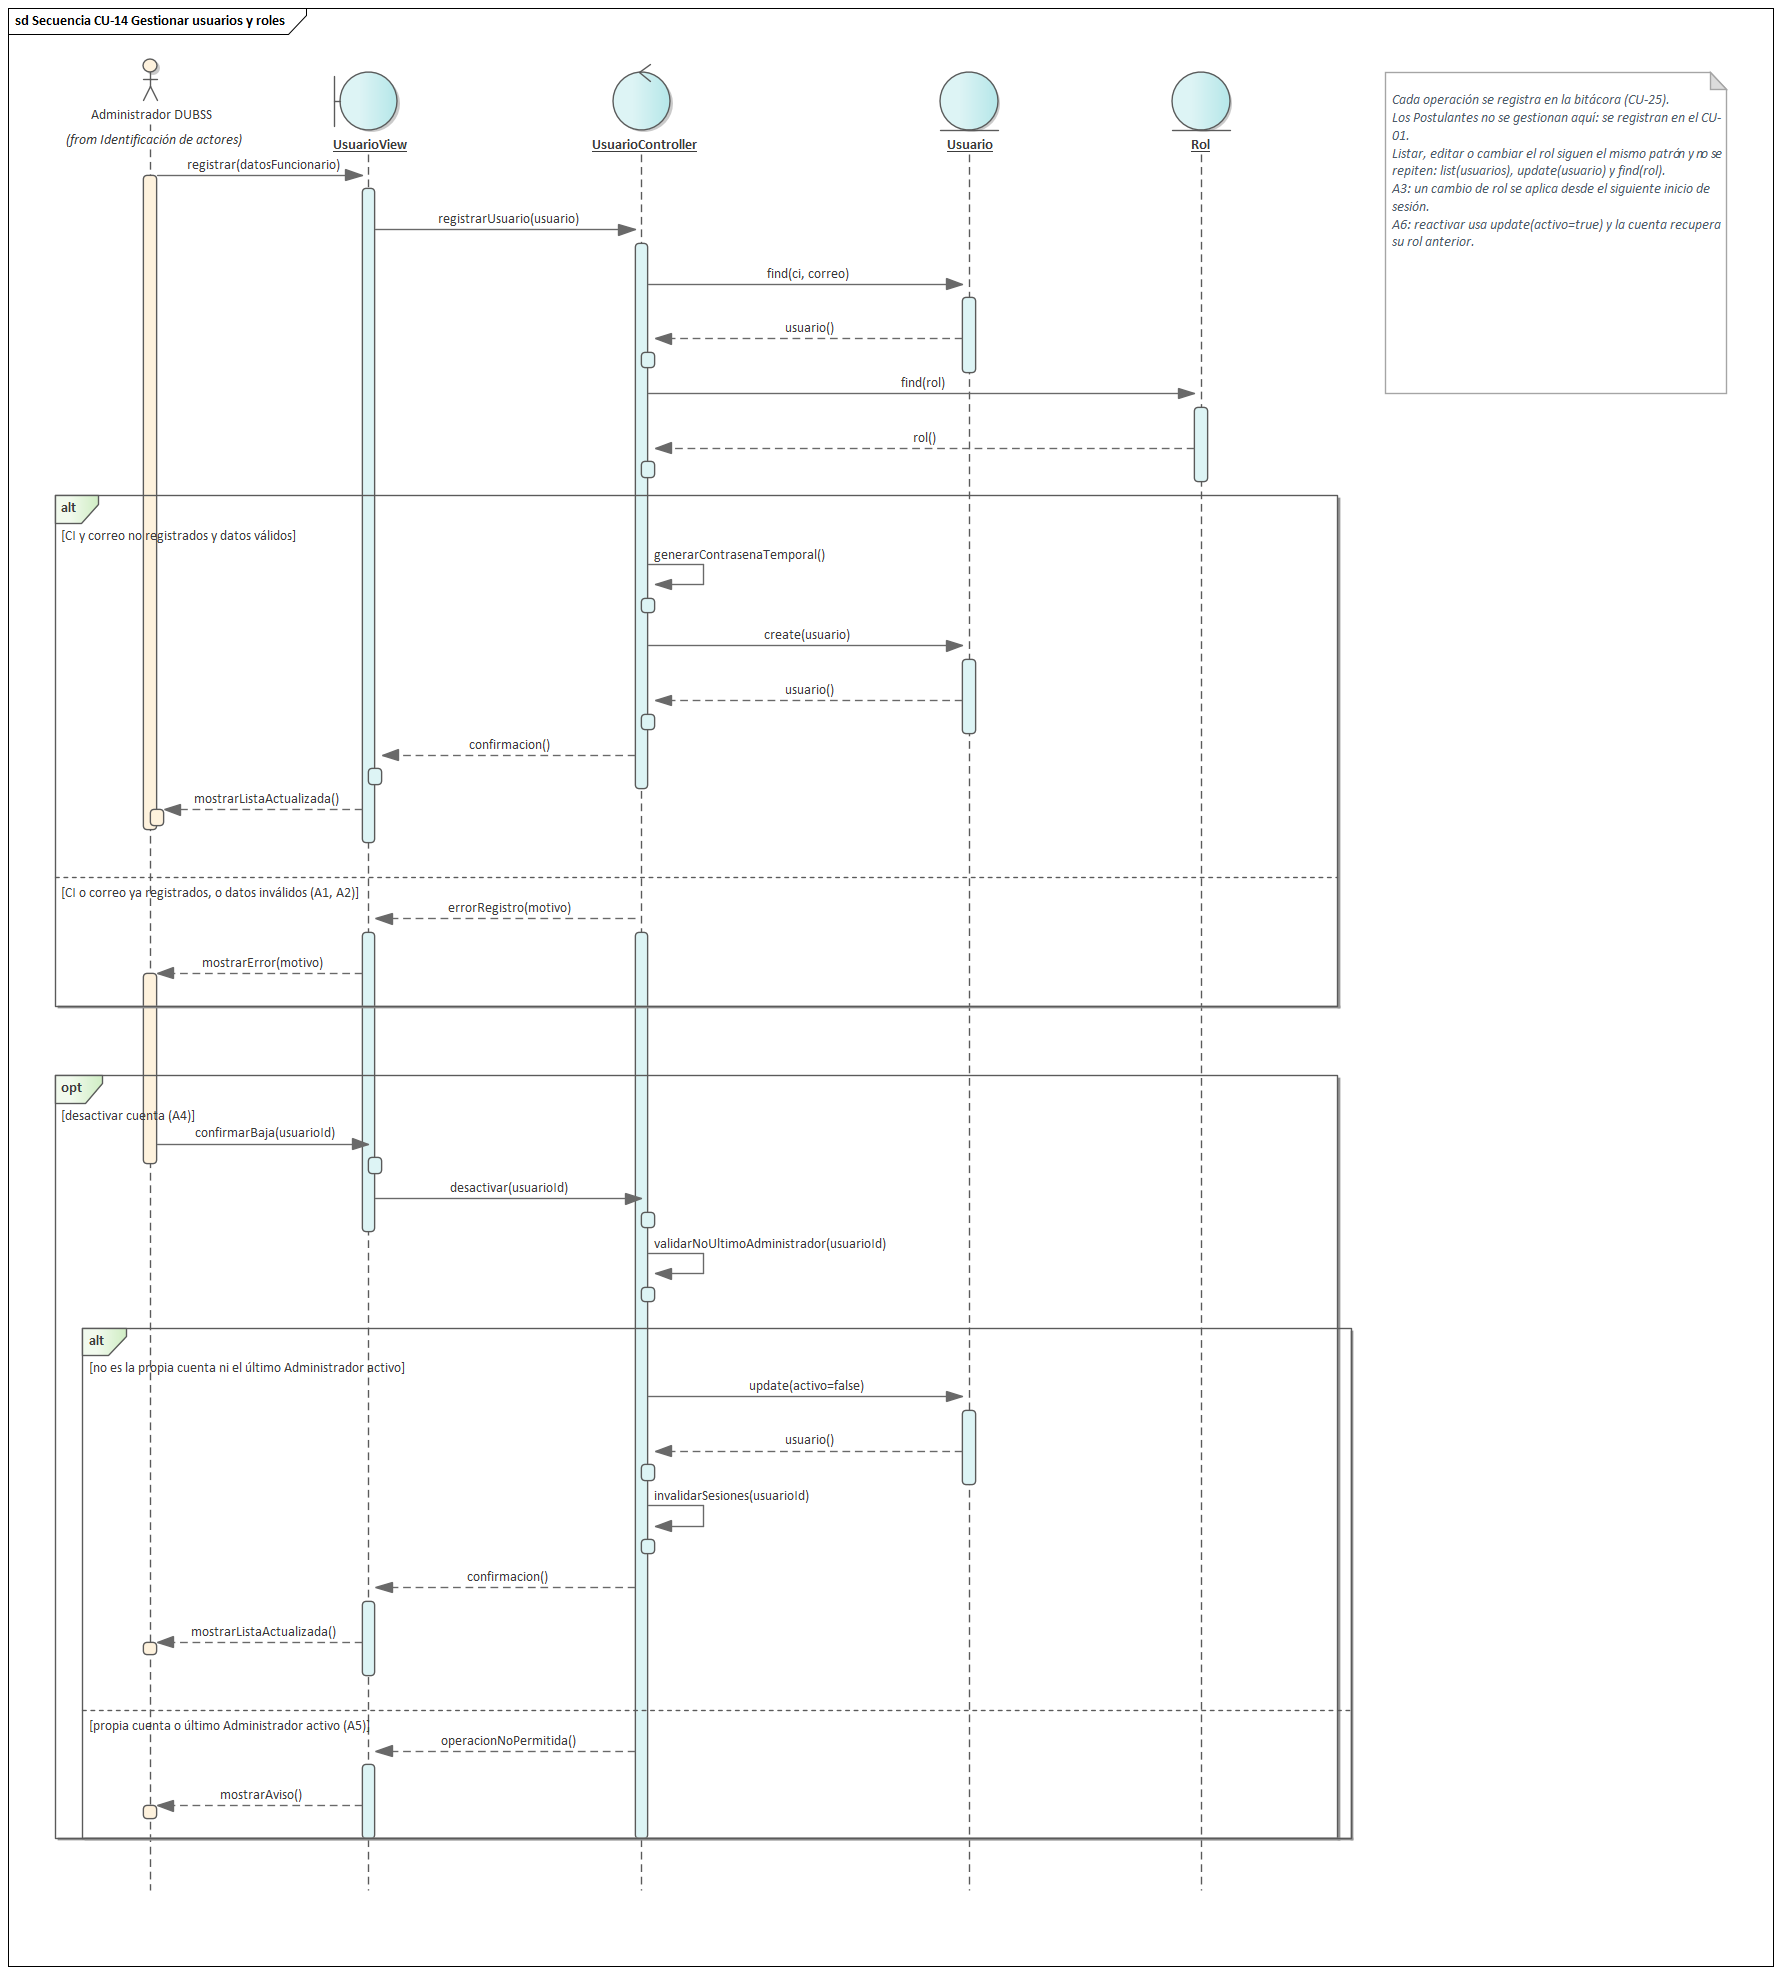
\includegraphics[width=\textwidth,height=0.75\textheight,keepaspectratio]{images/126_Secuencia_CU14_Gestionar_Usuarios_Roles.png}

\smallskip
\noindent\raggedright\textit{Nota.} Elaboración propia.
\end{figure}


\Needspace{0.9\textheight}
\subsubsection{7.4.15. Diseñar CU-15 Recuperar contraseña / gestionar perfil}\label{sec:cap7_disenar_cu15}

La Figura~\ref{fig:secuencia_cu15} presenta el diagrama de secuencia del CU-15.

\begin{figure}[H]
\caption{Diagrama de secuencia del CU-15 Recuperar contraseña / gestionar perfil}
\label{fig:secuencia_cu15}
\centering
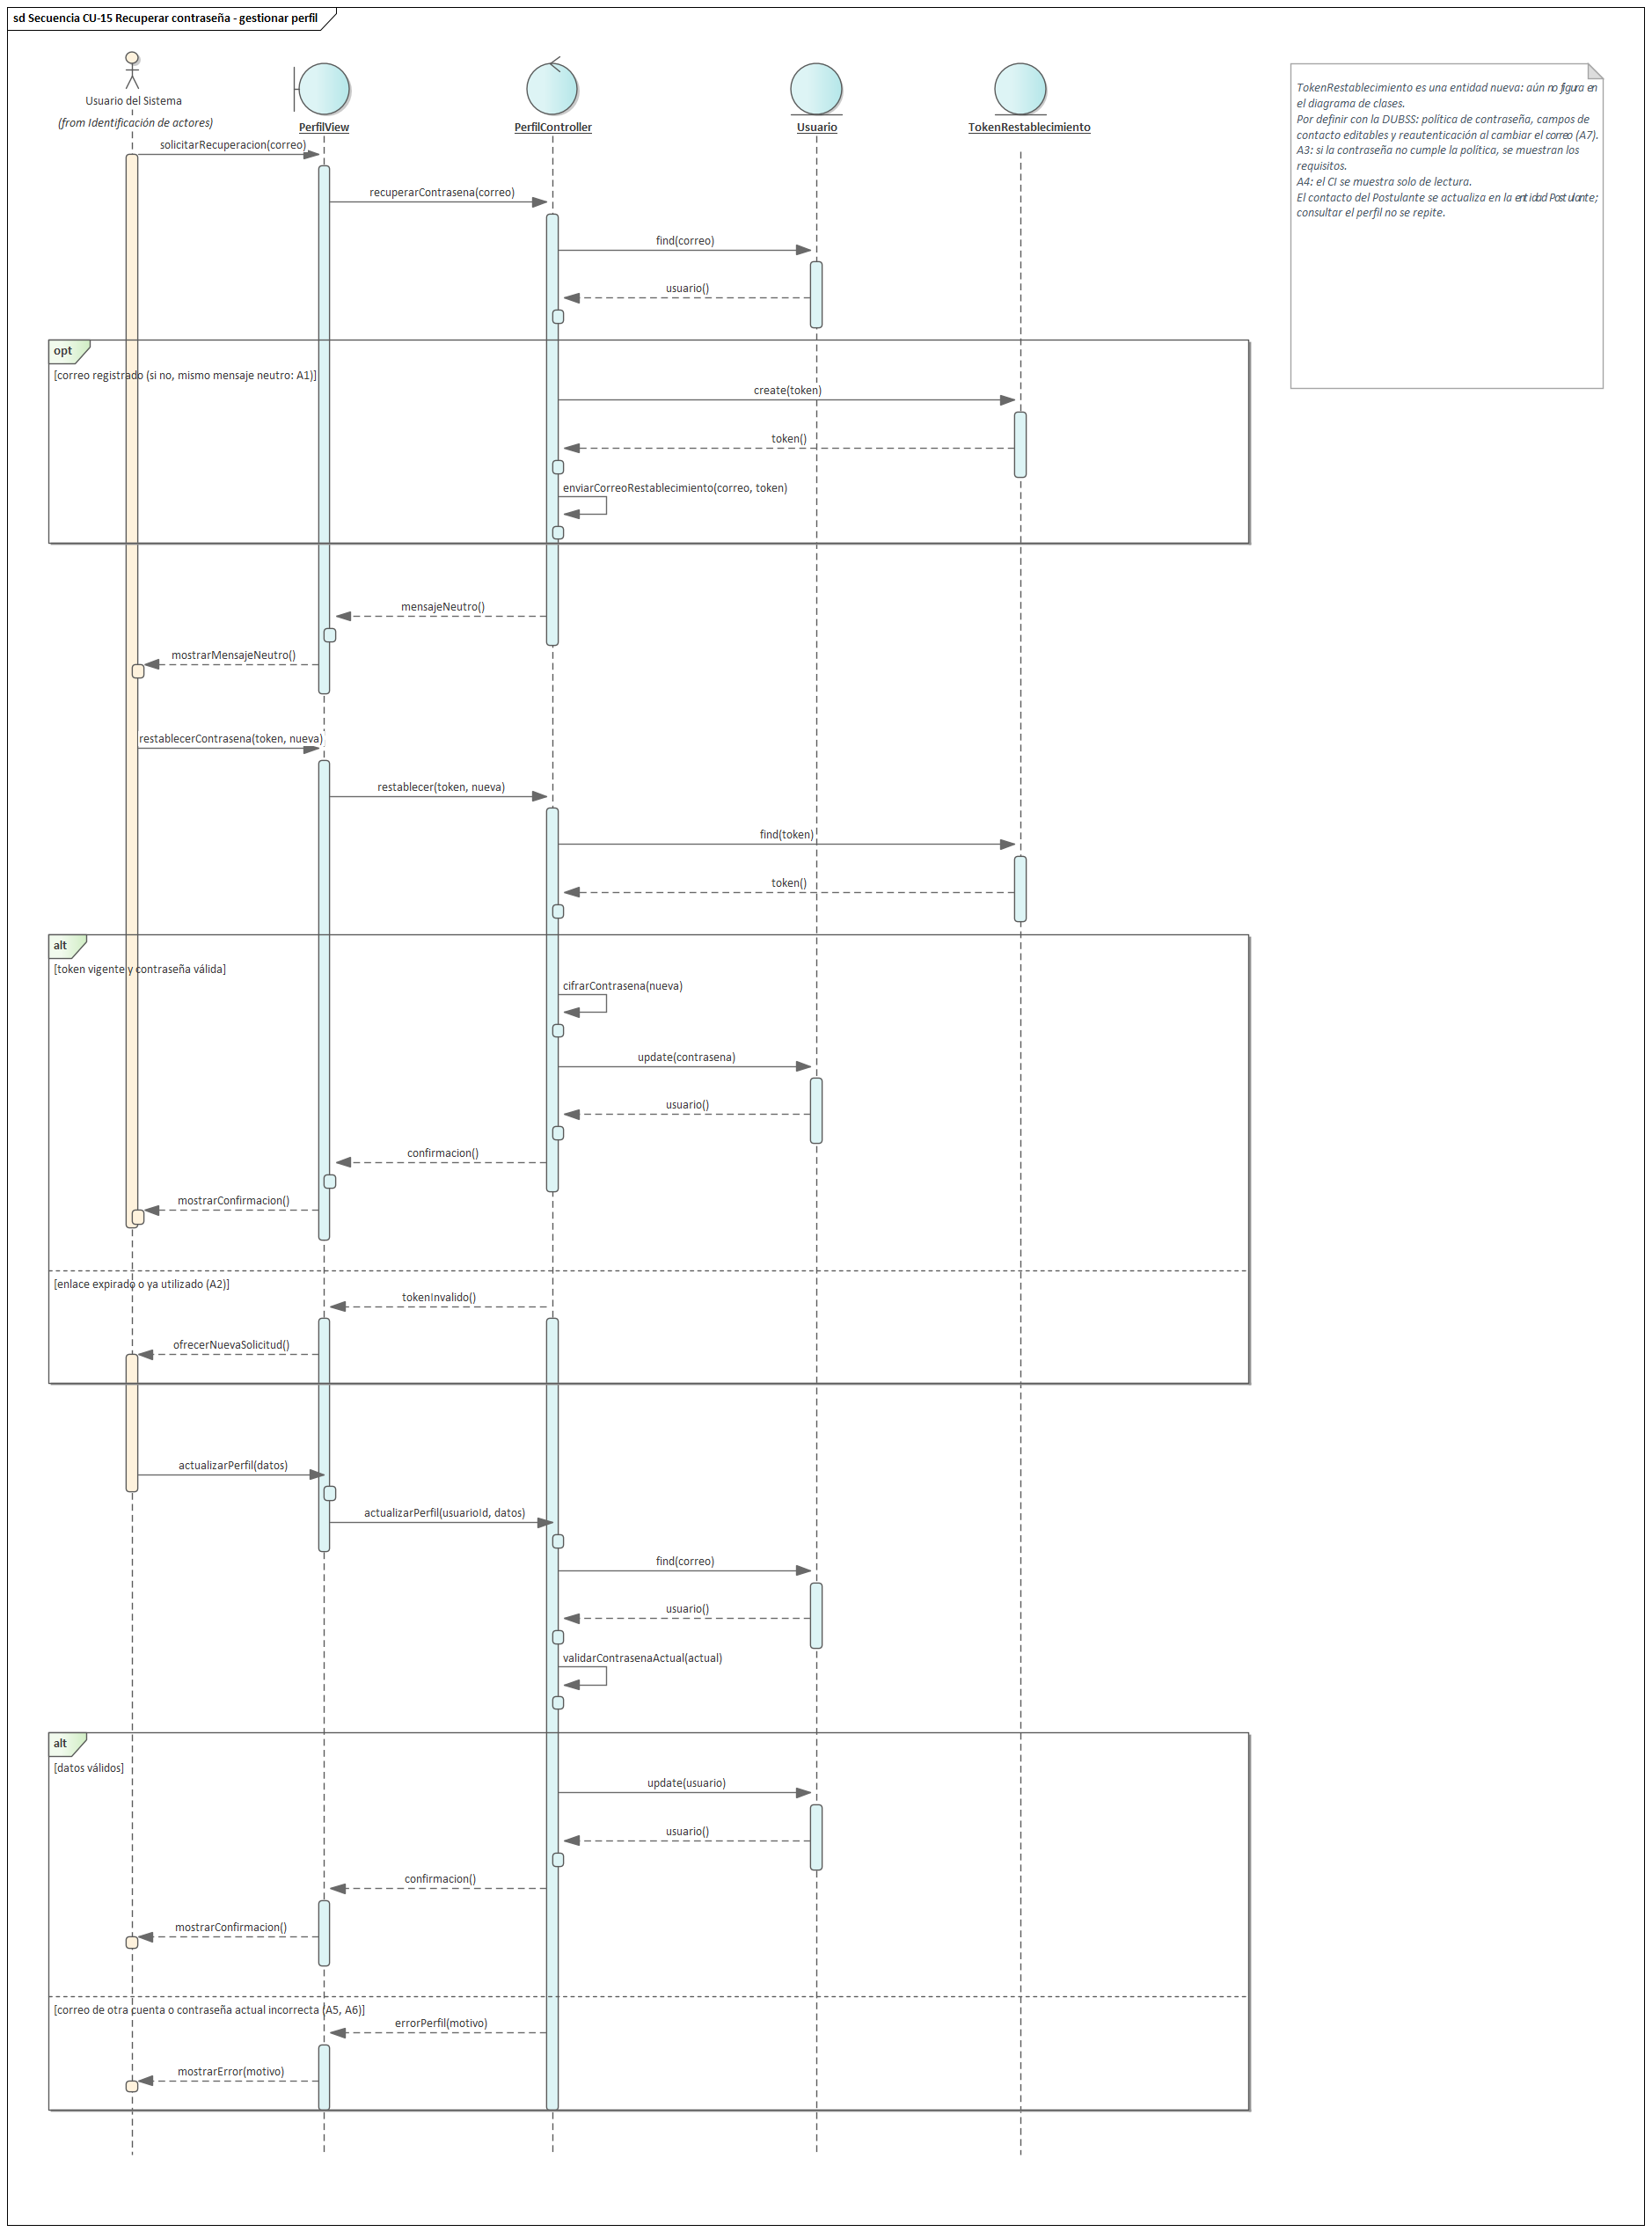
\includegraphics[width=\textwidth,height=0.75\textheight,keepaspectratio]{images/127_Secuencia_CU15_Recuperar_Contrasena_Gestionar_Perfil.png}

\smallskip
\noindent\raggedright\textit{Nota.} Elaboración propia.
\end{figure}


\Needspace{0.9\textheight}
\subsubsection{7.4.16. Diseñar CU-16 Digitalizar y adjuntar documentos}\label{sec:cap7_disenar_cu16}

La Figura~\ref{fig:secuencia_cu16} presenta el diagrama de secuencia del CU-16.

\begin{figure}[H]
\caption{Diagrama de secuencia del CU-16 Digitalizar y adjuntar documentos}
\label{fig:secuencia_cu16}
\centering
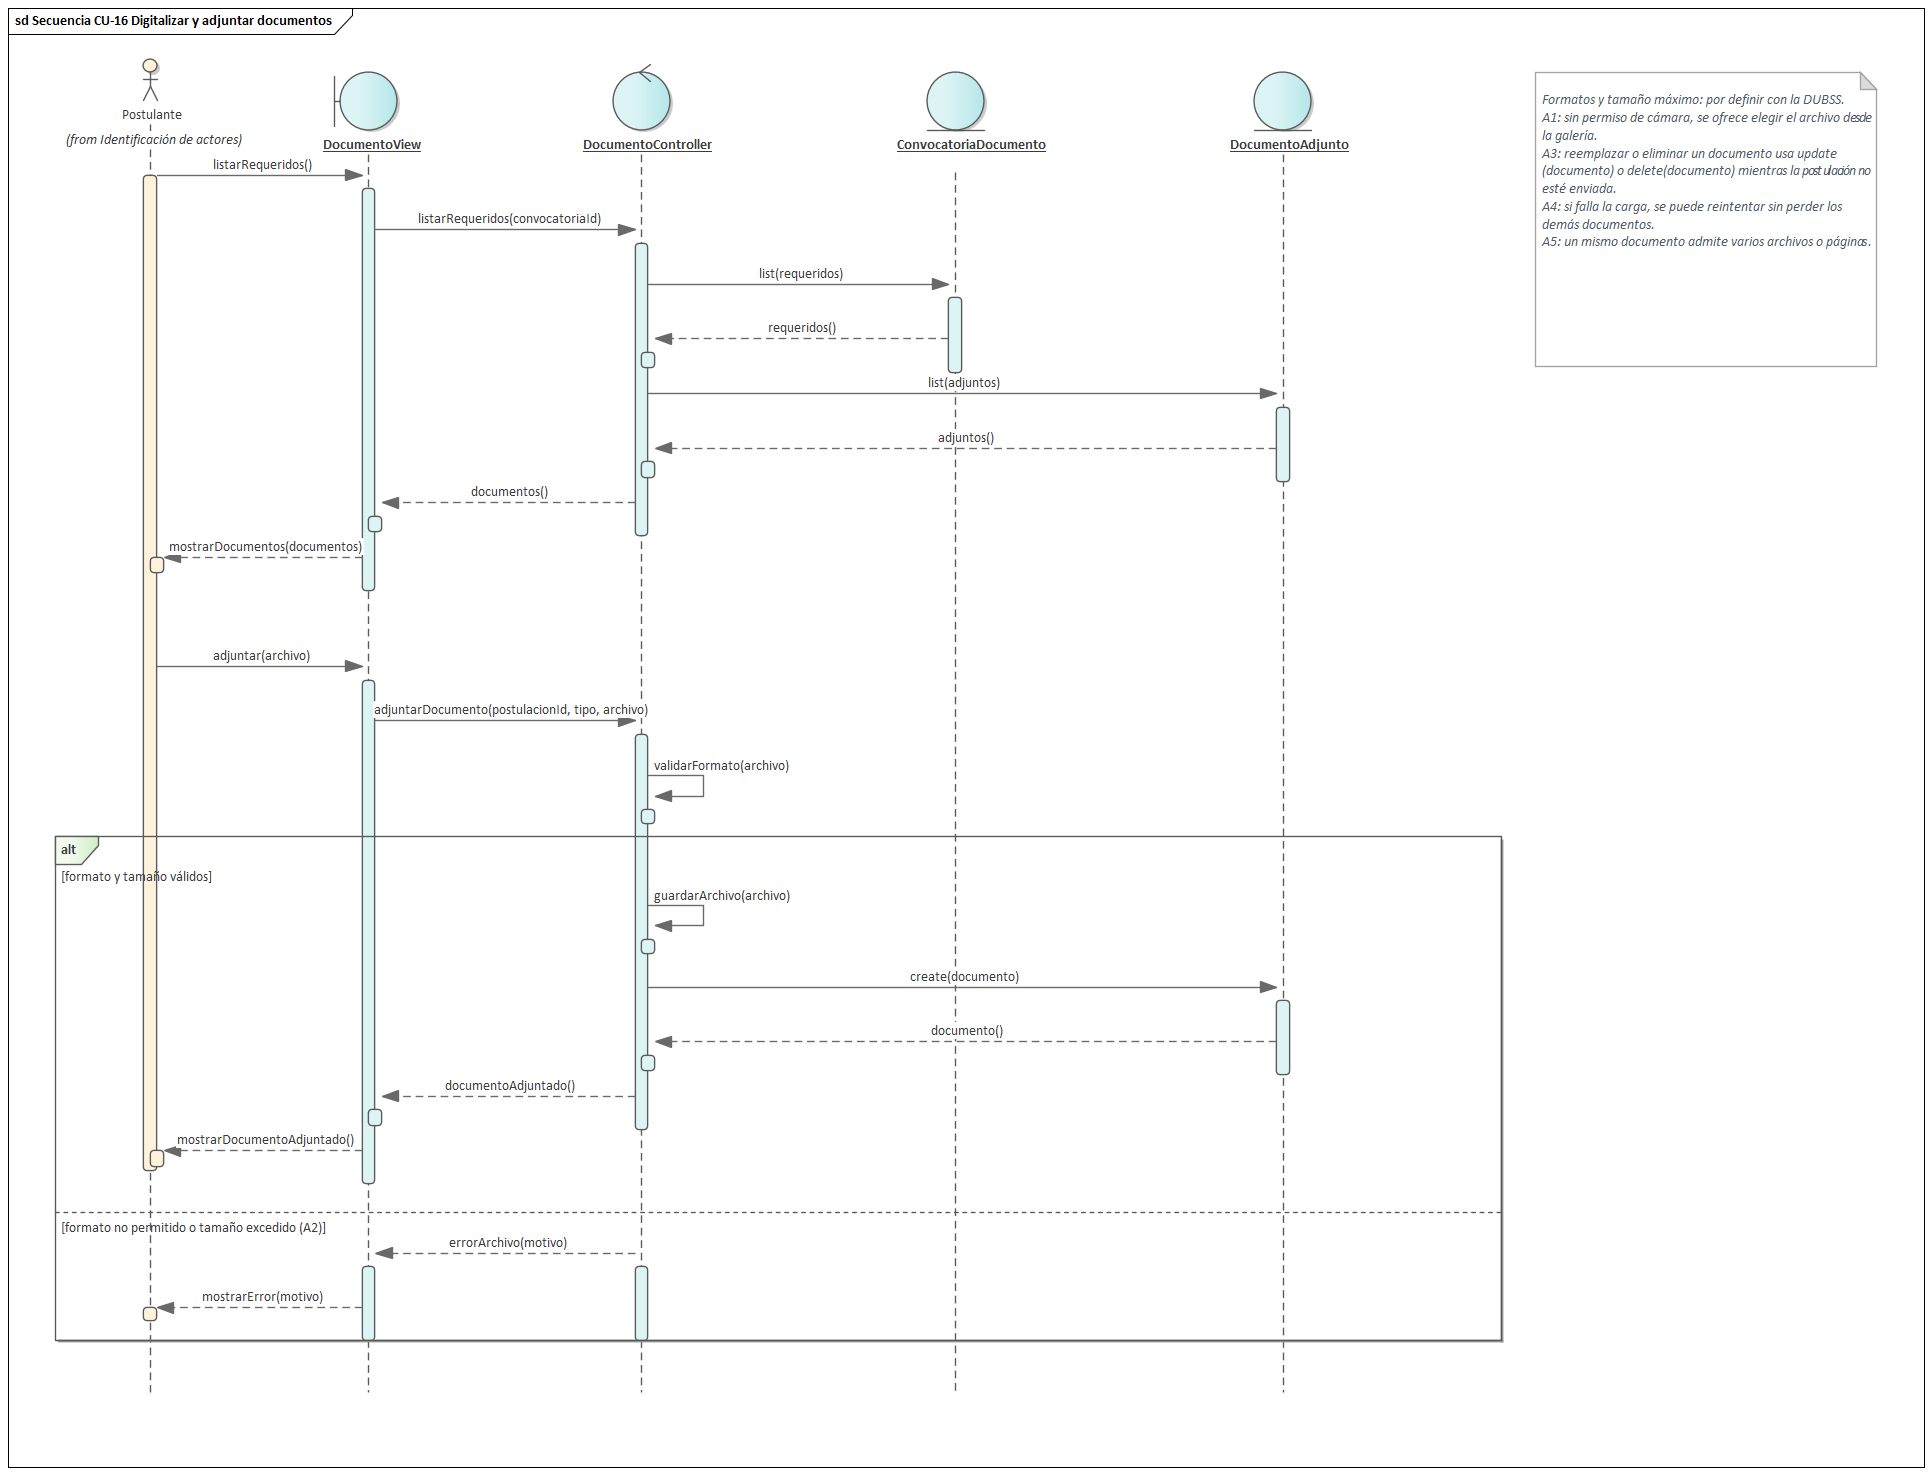
\includegraphics[width=\textwidth,height=0.75\textheight,keepaspectratio]{images/128_Secuencia_CU16_Digitalizar_Adjuntar_Documentos.png}

\smallskip
\noindent\raggedright\textit{Nota.} Elaboración propia.
\end{figure}


\Needspace{0.9\textheight}
\subsubsection{7.4.17. Diseñar CU-17 Guardar borrador de postulación}\label{sec:cap7_disenar_cu17}

La Figura~\ref{fig:secuencia_cu17} presenta el diagrama de secuencia del CU-17.

\begin{figure}[H]
\caption{Diagrama de secuencia del CU-17 Guardar borrador de postulación}
\label{fig:secuencia_cu17}
\centering
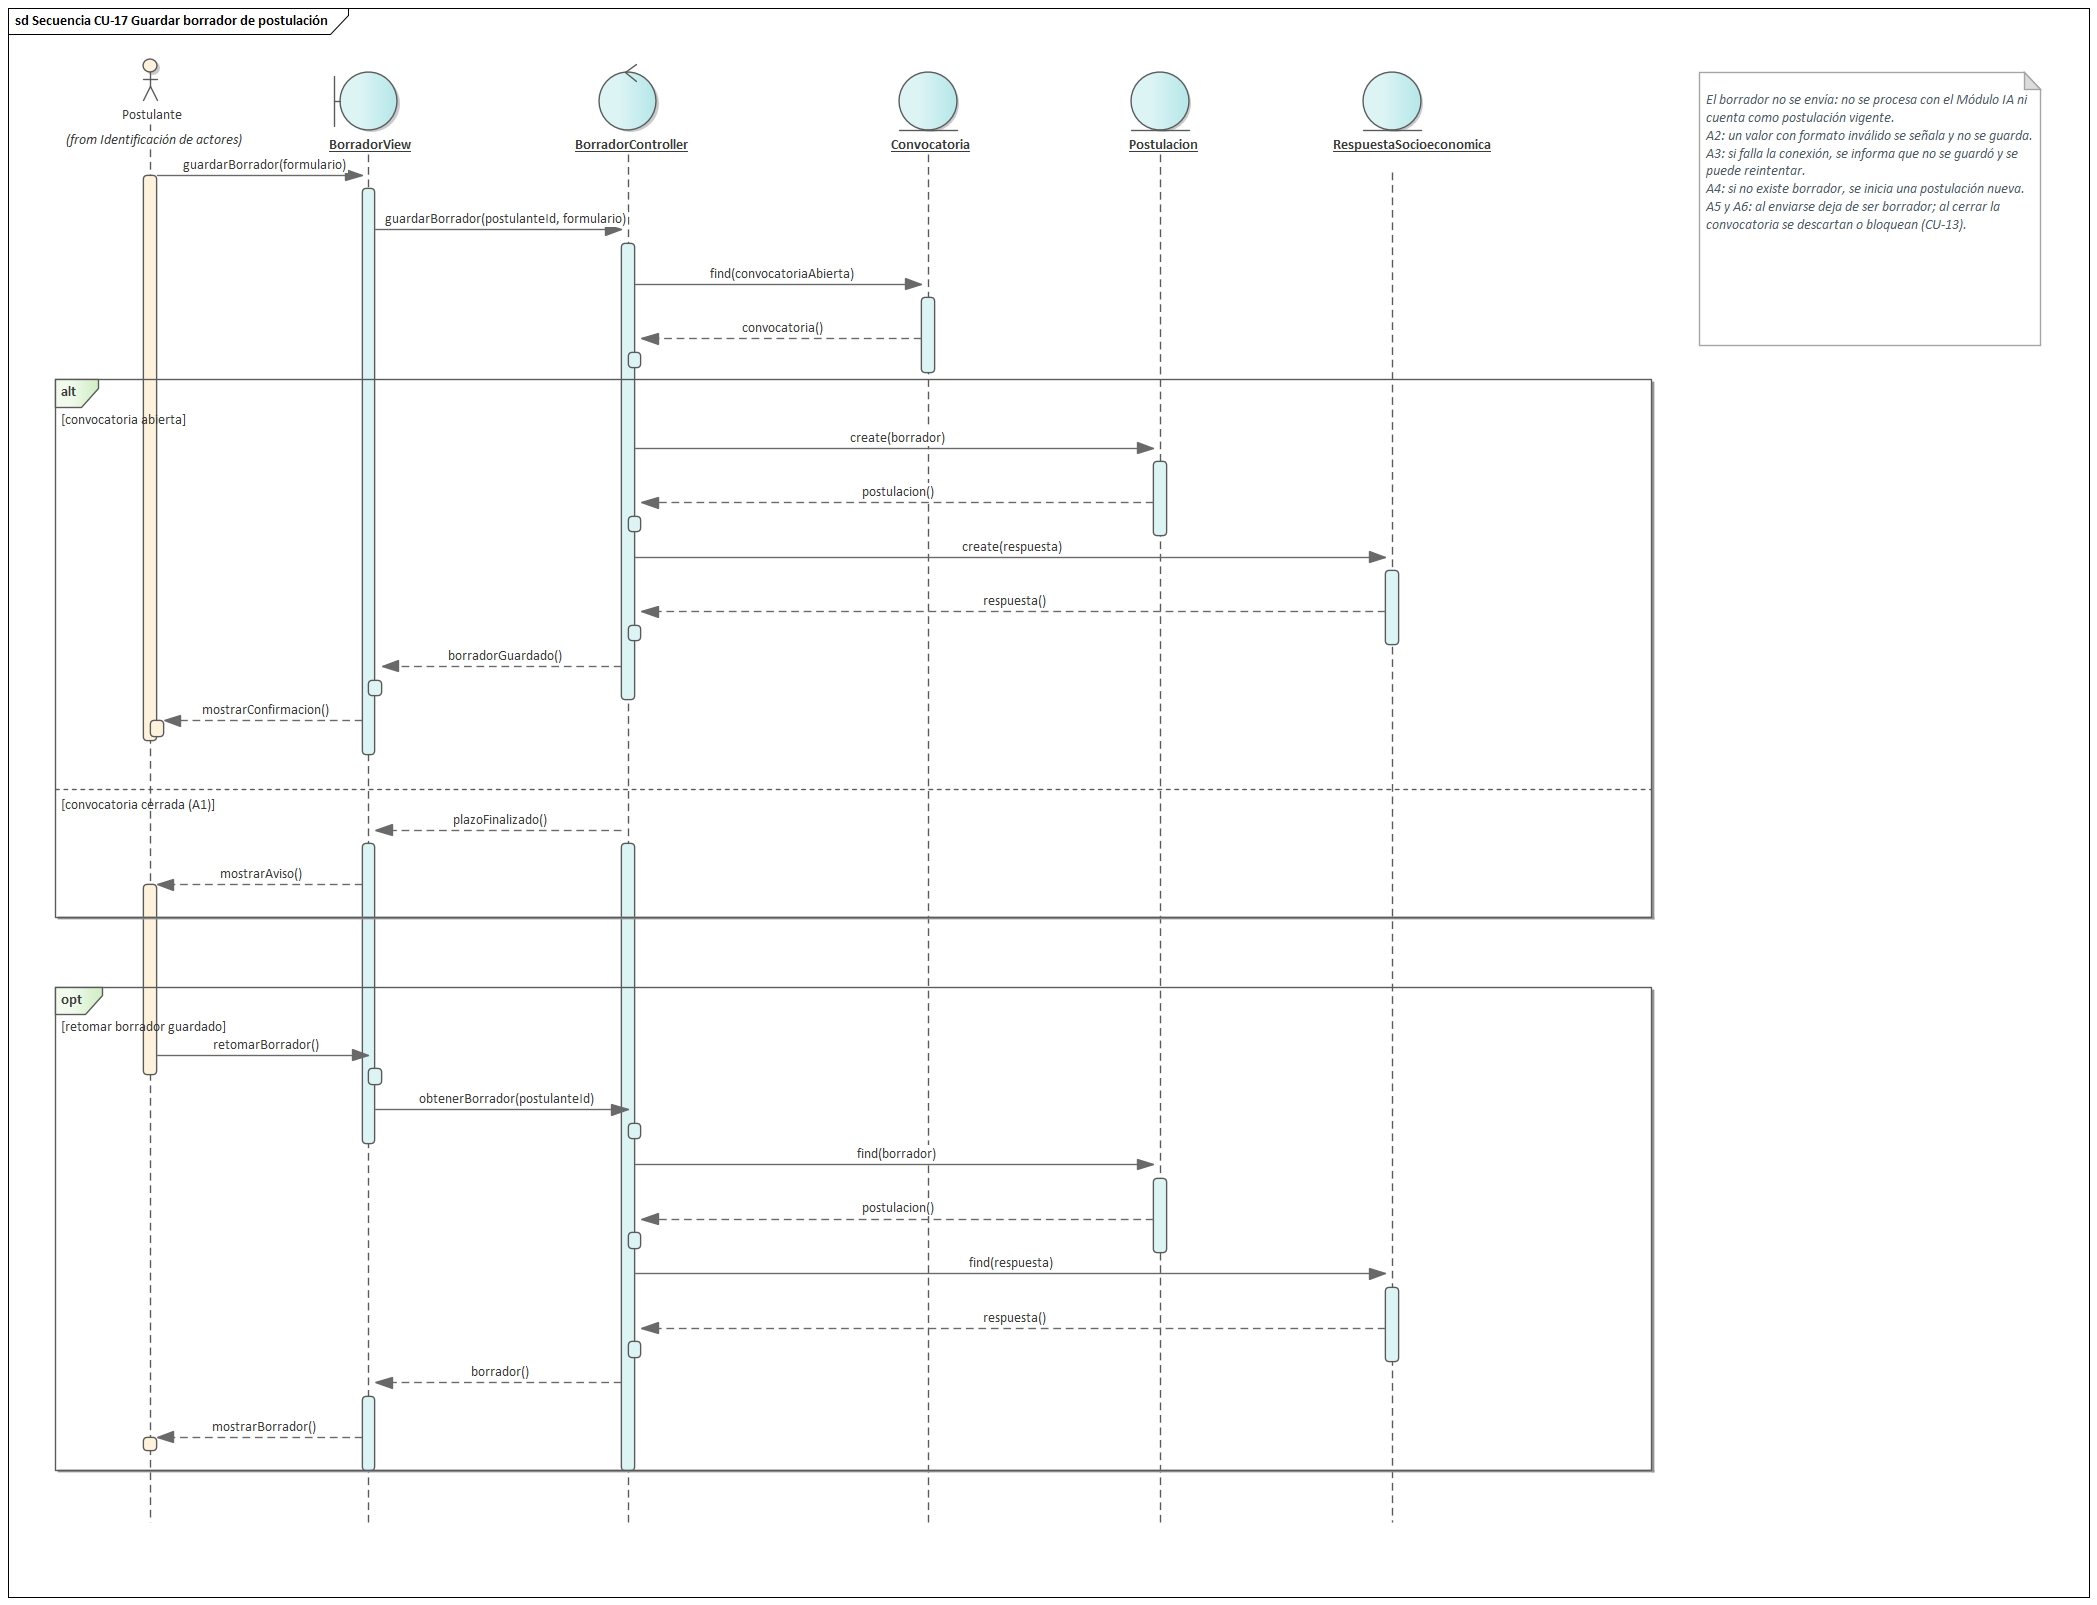
\includegraphics[width=\textwidth,height=0.75\textheight,keepaspectratio]{images/129_Secuencia_CU17_Guardar_Borrador_Postulacion.png}

\smallskip
\noindent\raggedright\textit{Nota.} Elaboración propia.
\end{figure}


\Needspace{0.9\textheight}
\subsubsection{7.4.18. Diseñar CU-18 Validar elegibilidad y duplicados}\label{sec:cap7_disenar_cu18}

La Figura~\ref{fig:secuencia_cu18} presenta el diagrama de secuencia del CU-18.

\begin{figure}[H]
\caption{Diagrama de secuencia del CU-18 Validar elegibilidad y duplicados}
\label{fig:secuencia_cu18}
\centering
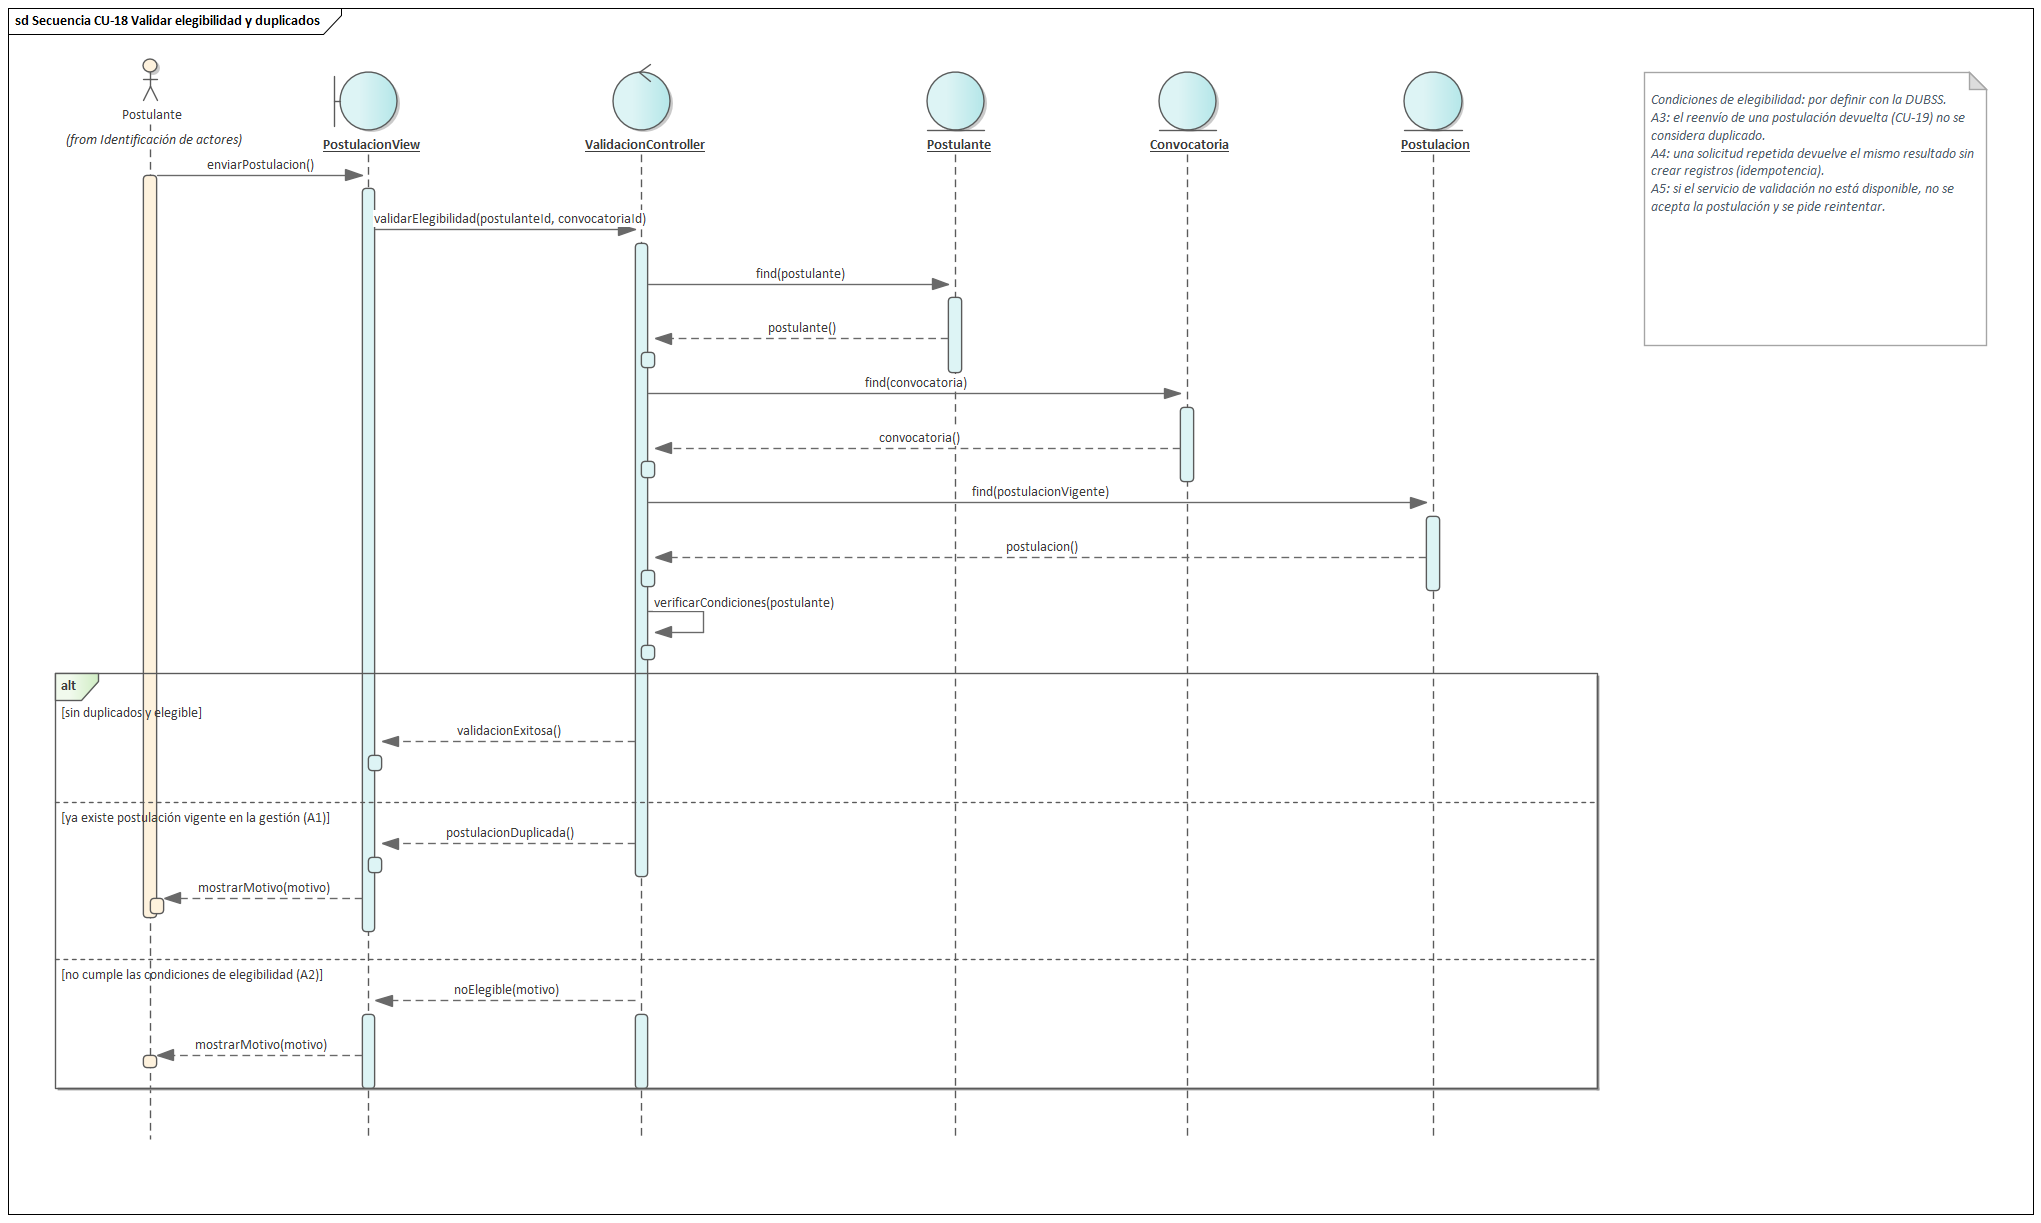
\includegraphics[width=\textwidth,height=0.75\textheight,keepaspectratio]{images/130_Secuencia_CU18_Validar_Elegibilidad_Duplicados.png}

\smallskip
\noindent\raggedright\textit{Nota.} Elaboración propia.
\end{figure}


\Needspace{0.9\textheight}
\subsubsection{7.4.19. Diseñar CU-19 Devolver postulación para corrección}\label{sec:cap7_disenar_cu19}

La Figura~\ref{fig:secuencia_cu19} presenta el diagrama de secuencia del CU-19.

\begin{figure}[H]
\caption{Diagrama de secuencia del CU-19 Devolver postulación para corrección}
\label{fig:secuencia_cu19}
\centering
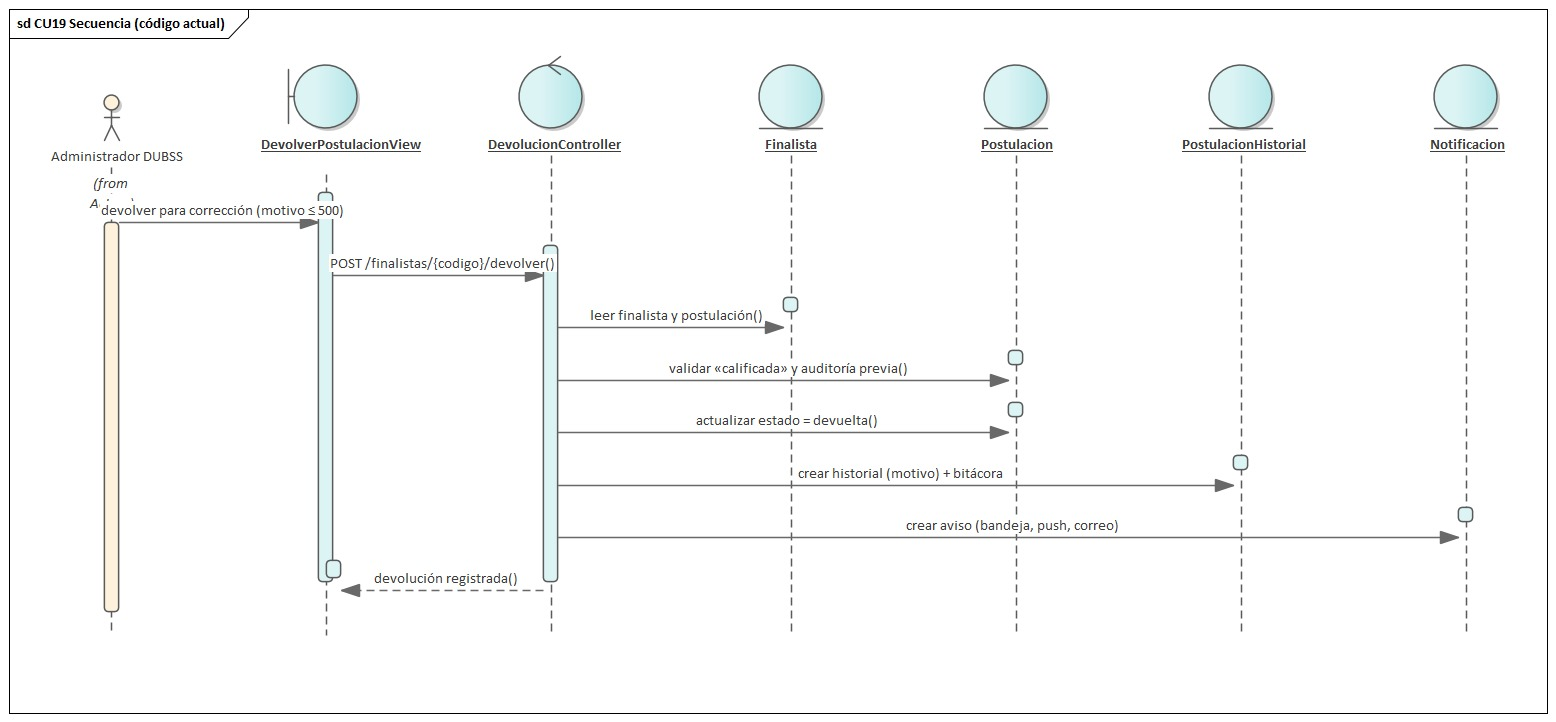
\includegraphics[width=\textwidth,height=0.75\textheight,keepaspectratio]{images/100_Secuencia_CU19_Devolver_Postulacion_Correccion.jpg}

\smallskip
\noindent\raggedright\textit{Nota.} Elaboración propia.
\end{figure}


\Needspace{0.9\textheight}
\subsubsection{7.4.20. Diseñar CU-20 Archivar o rechazar postulación}\label{sec:cap7_disenar_cu20}

La Figura~\ref{fig:secuencia_cu20} presenta el diagrama de secuencia del CU-20.

\begin{figure}[H]
\caption{Diagrama de secuencia del CU-20 Archivar o rechazar postulación}
\label{fig:secuencia_cu20}
\centering
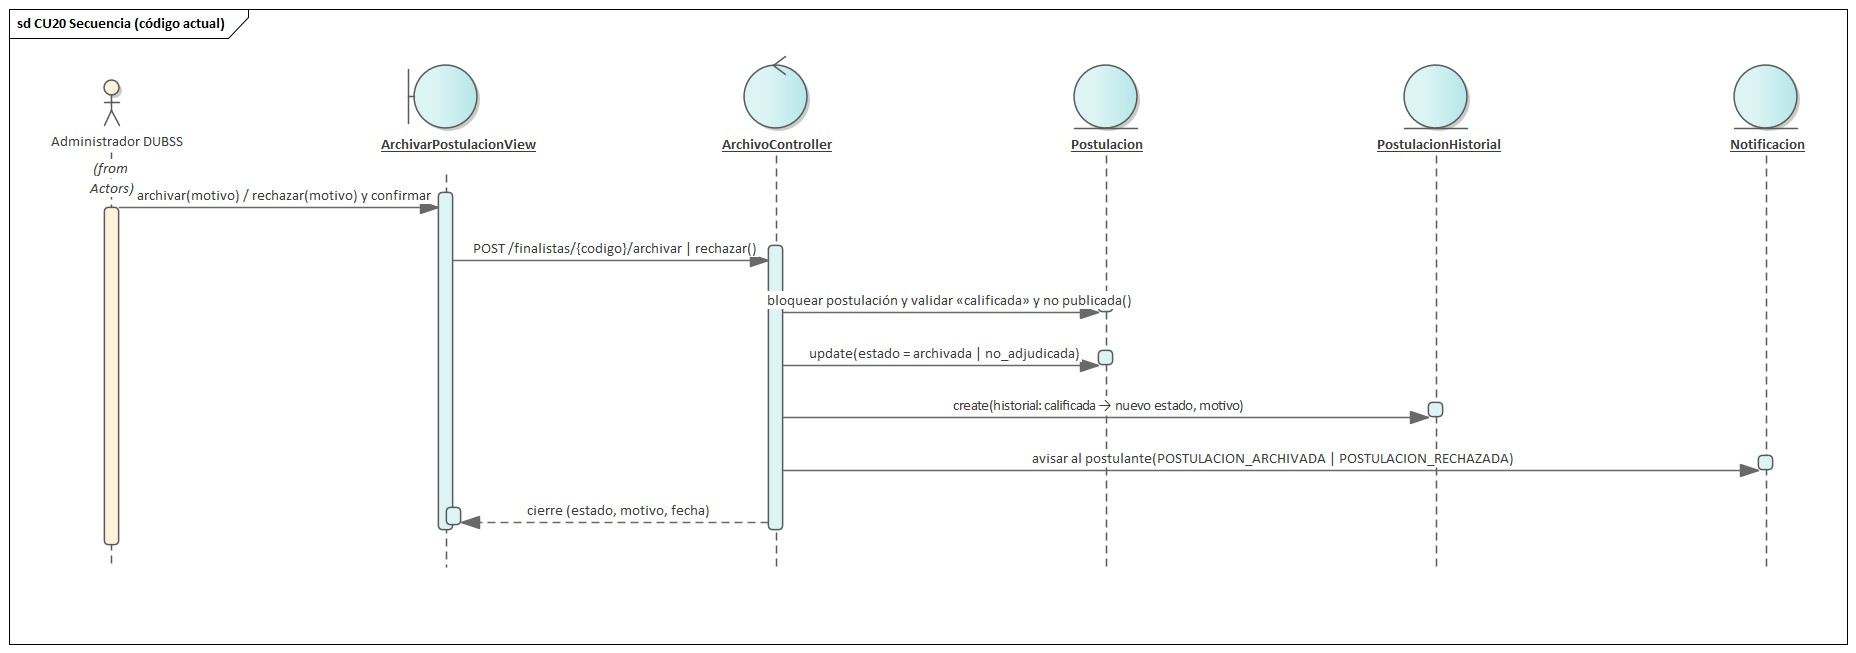
\includegraphics[width=\textwidth,height=0.75\textheight,keepaspectratio]{images/101_Secuencia_CU20_Archivar_Rechazar_Postulacion.jpg}

\smallskip
\noindent\raggedright\textit{Nota.} Elaboración propia.
\end{figure}


\Needspace{0.9\textheight}
\subsubsection{7.4.21. Diseñar CU-21 Notificar finalistas, registrar entrega de documentación física y publicar comunicados/avisos}\label{sec:cap7_disenar_cu21}

La Figura~\ref{fig:secuencia_cu21} presenta el diagrama de secuencia del CU-21.

\begin{figure}[H]
\caption{Diagrama de secuencia del CU-21 Notificar finalistas, registrar entrega de documentación física y publicar comunicados/avisos}
\label{fig:secuencia_cu21}
\centering
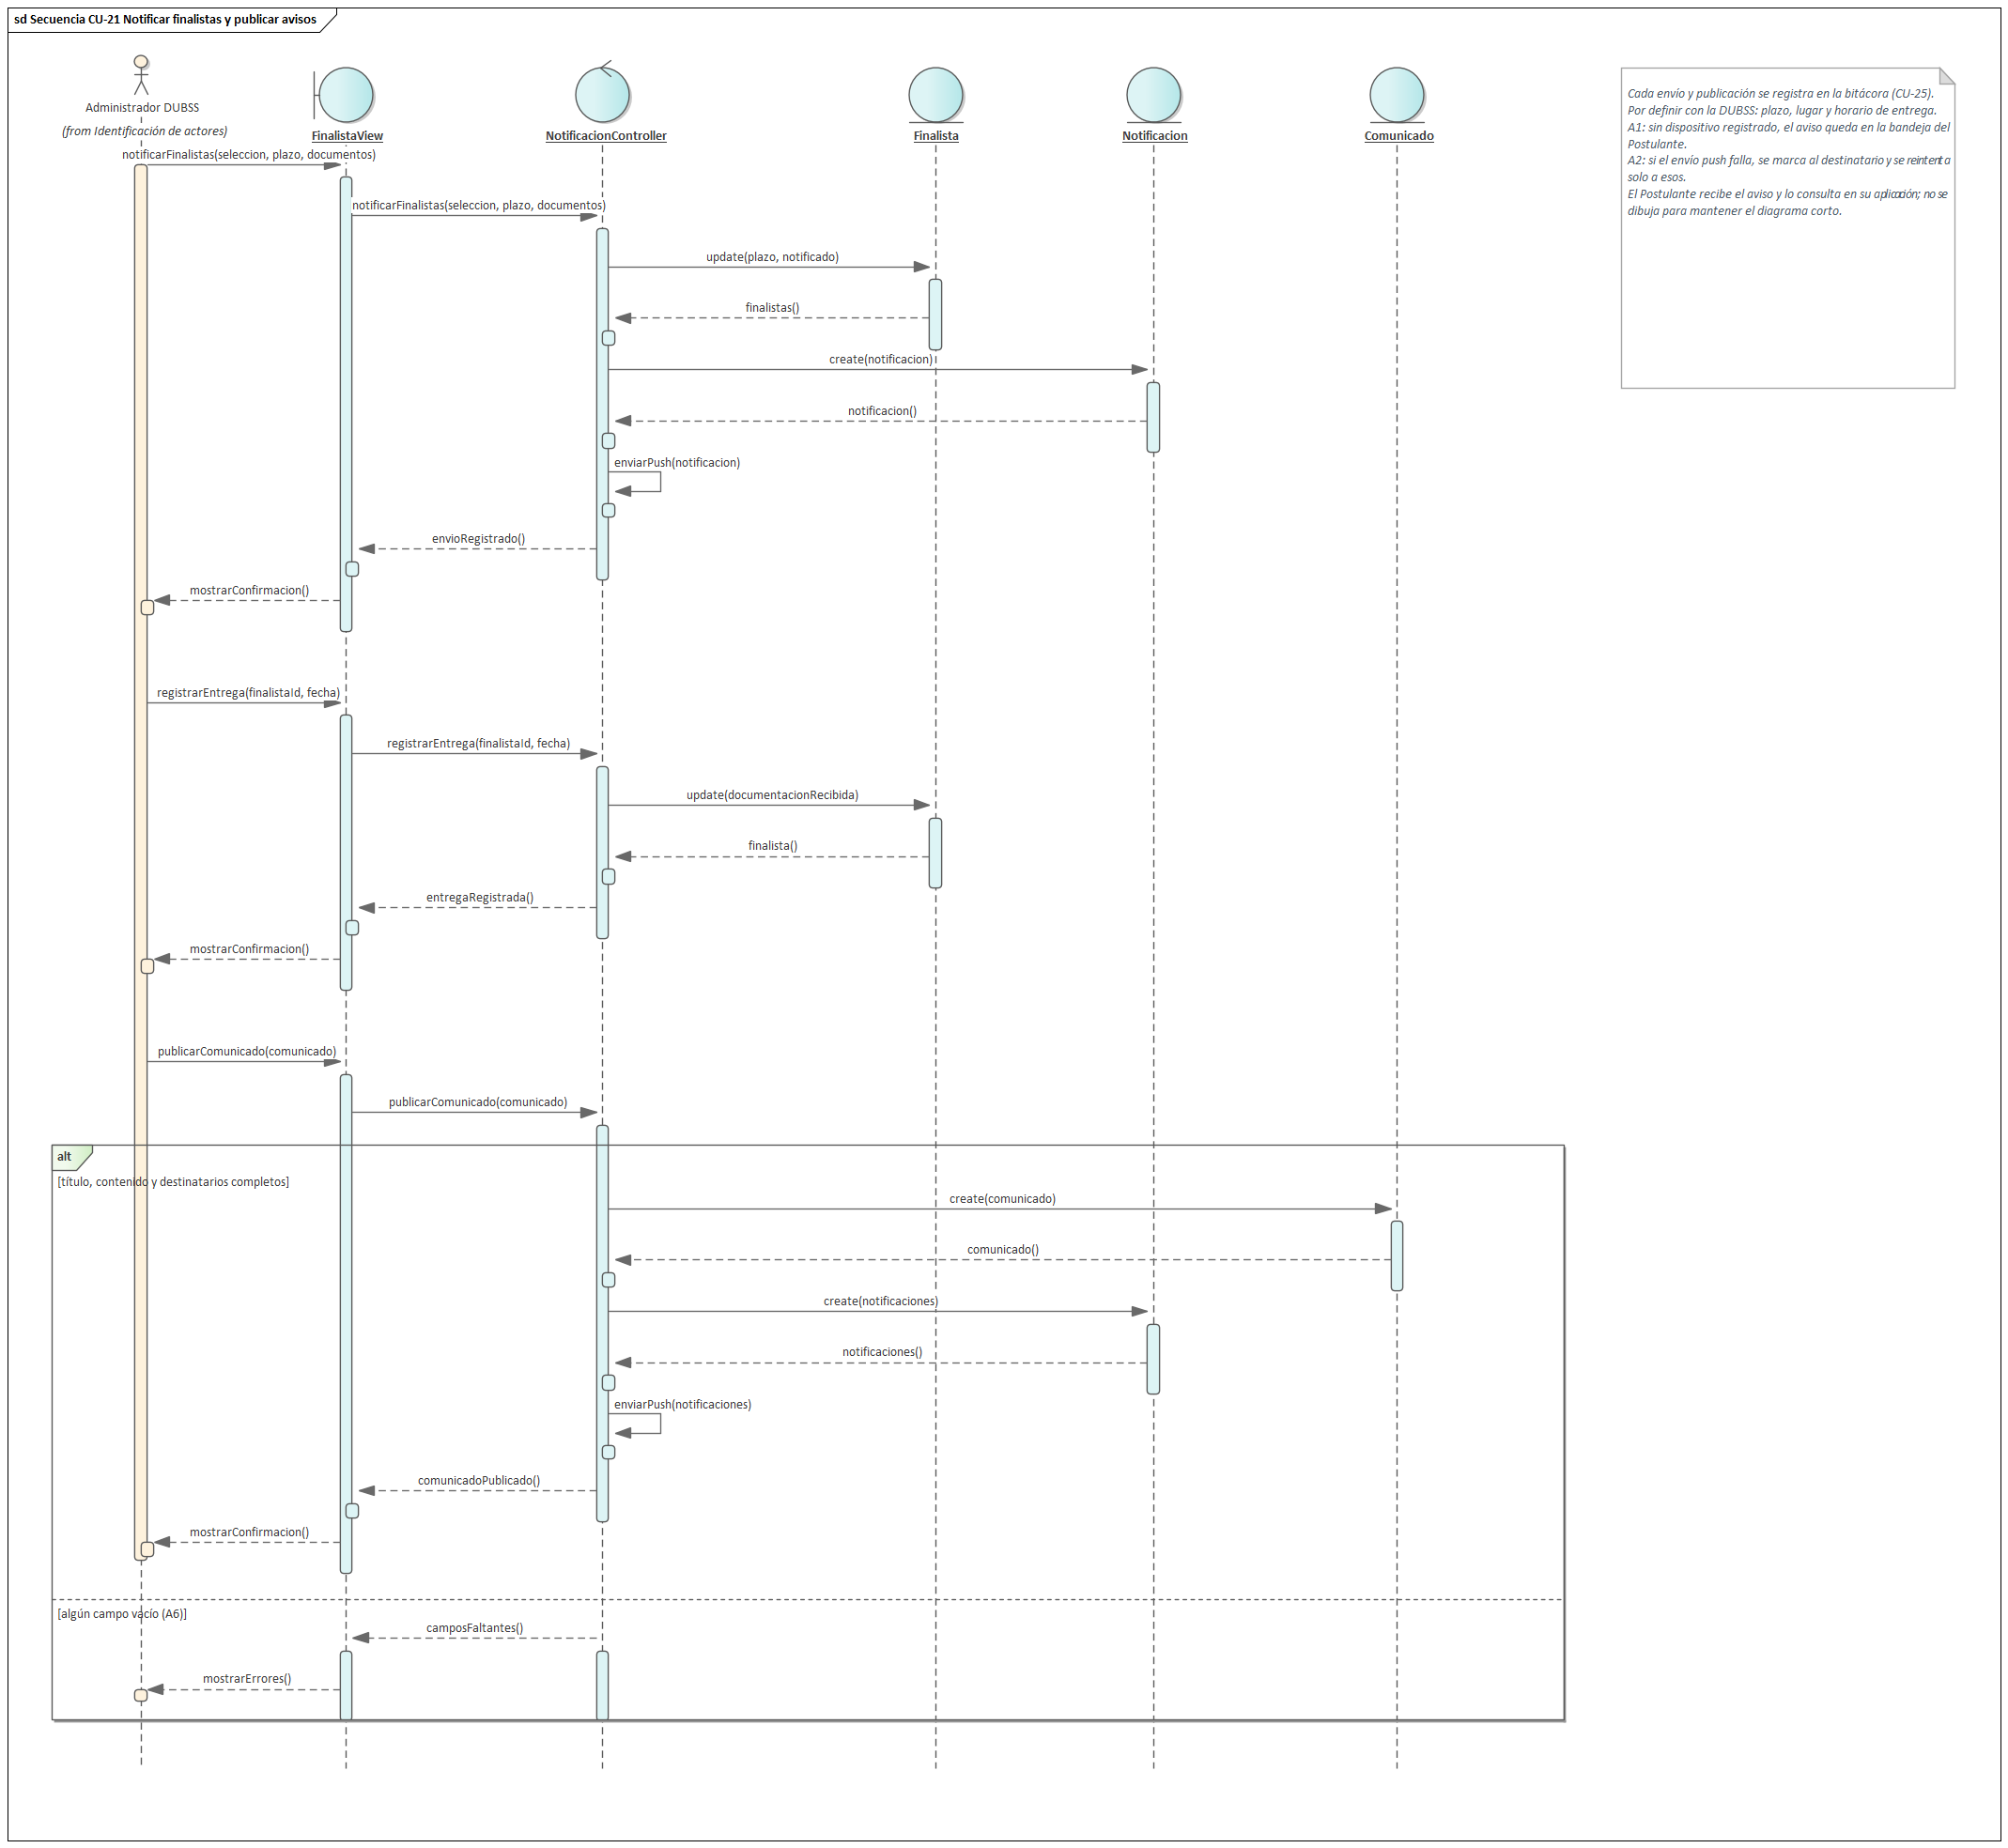
\includegraphics[width=\textwidth,height=0.75\textheight,keepaspectratio]{images/131_Secuencia_CU21_Notificar_Finalistas_Publicar_Avisos.png}

\smallskip
\noindent\raggedright\textit{Nota.} Elaboración propia.
\end{figure}


\Needspace{0.9\textheight}
\subsubsection{7.4.22. Diseñar CU-22 Publicar resultados de adjudicación}\label{sec:cap7_disenar_cu22}

La Figura~\ref{fig:secuencia_cu22} presenta el diagrama de secuencia del CU-22.

\begin{figure}[H]
\caption{Diagrama de secuencia del CU-22 Publicar resultados de adjudicación}
\label{fig:secuencia_cu22}
\centering
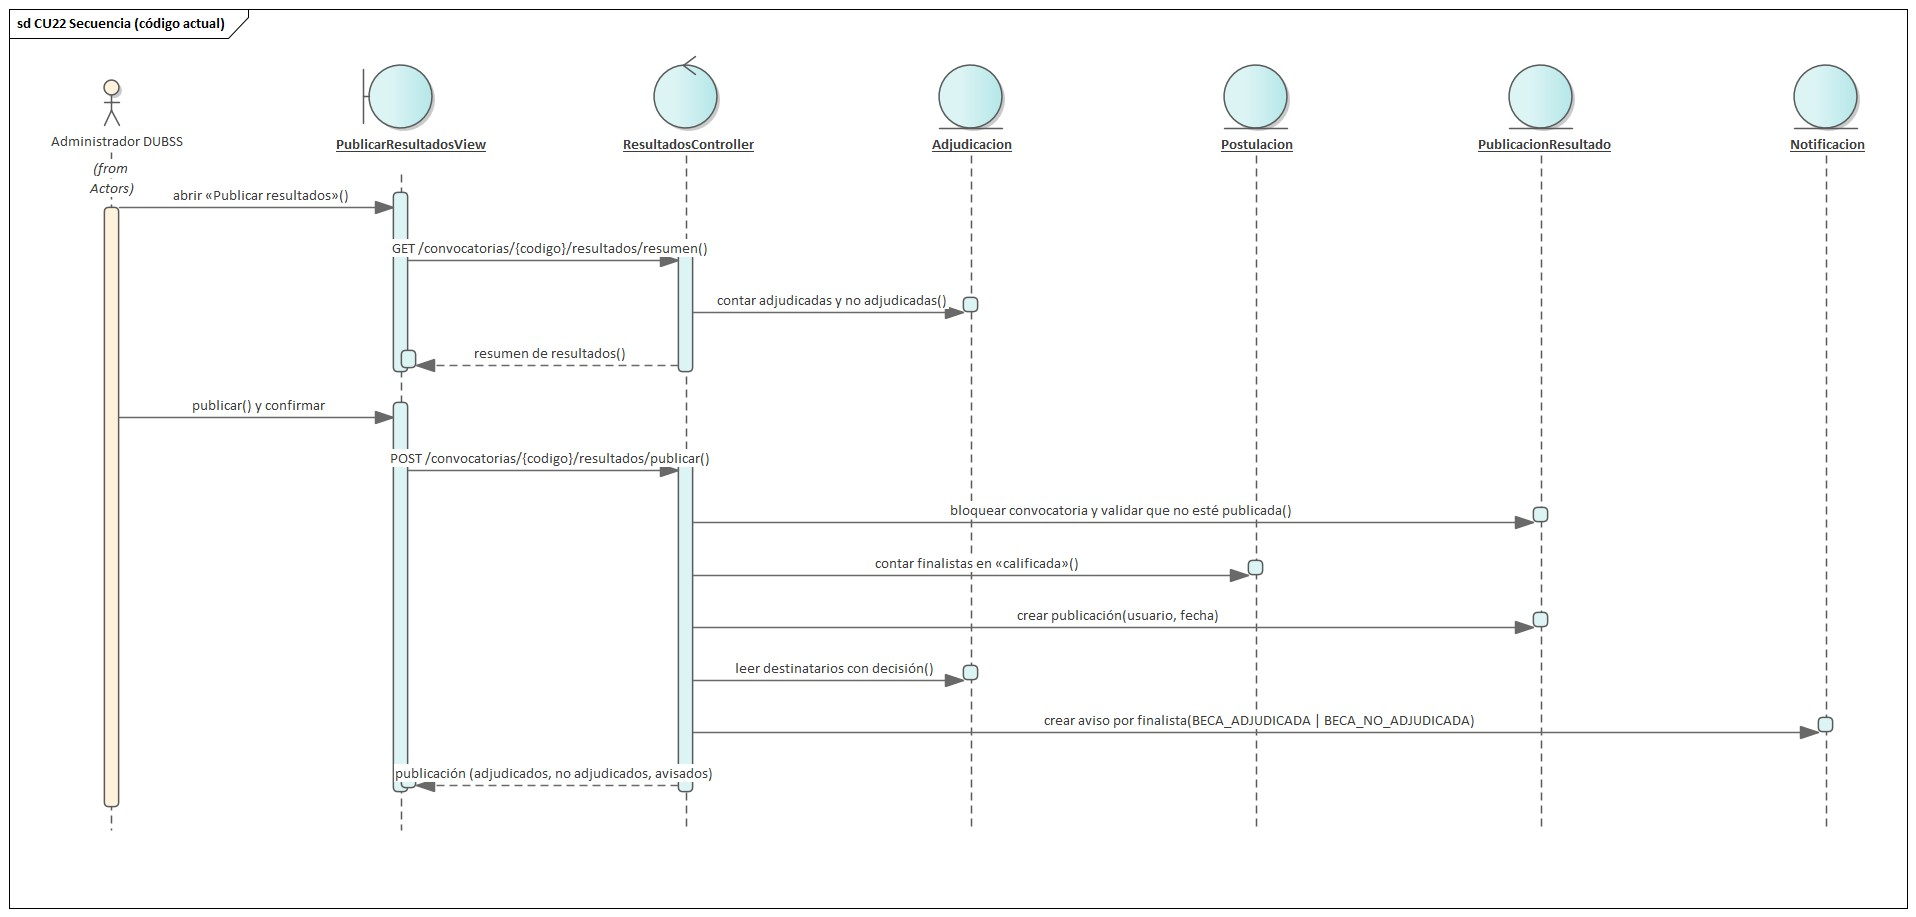
\includegraphics[width=\textwidth,height=0.75\textheight,keepaspectratio]{images/102_Secuencia_CU22_Publicar_Resultados_Adjudicacion.jpg}

\smallskip
\noindent\raggedright\textit{Nota.} Elaboración propia.
\end{figure}


\Needspace{0.9\textheight}
\subsubsection{7.4.23. Diseñar CU-23 Gestionar padrón de becados (baja, suspensión, reemplazo)}\label{sec:cap7_disenar_cu23}

La Figura~\ref{fig:secuencia_cu23} presenta el diagrama de secuencia del CU-23.

\begin{figure}[H]
\caption{Diagrama de secuencia del CU-23 Gestionar padrón de becados (baja, suspensión, reemplazo)}
\label{fig:secuencia_cu23}
\centering
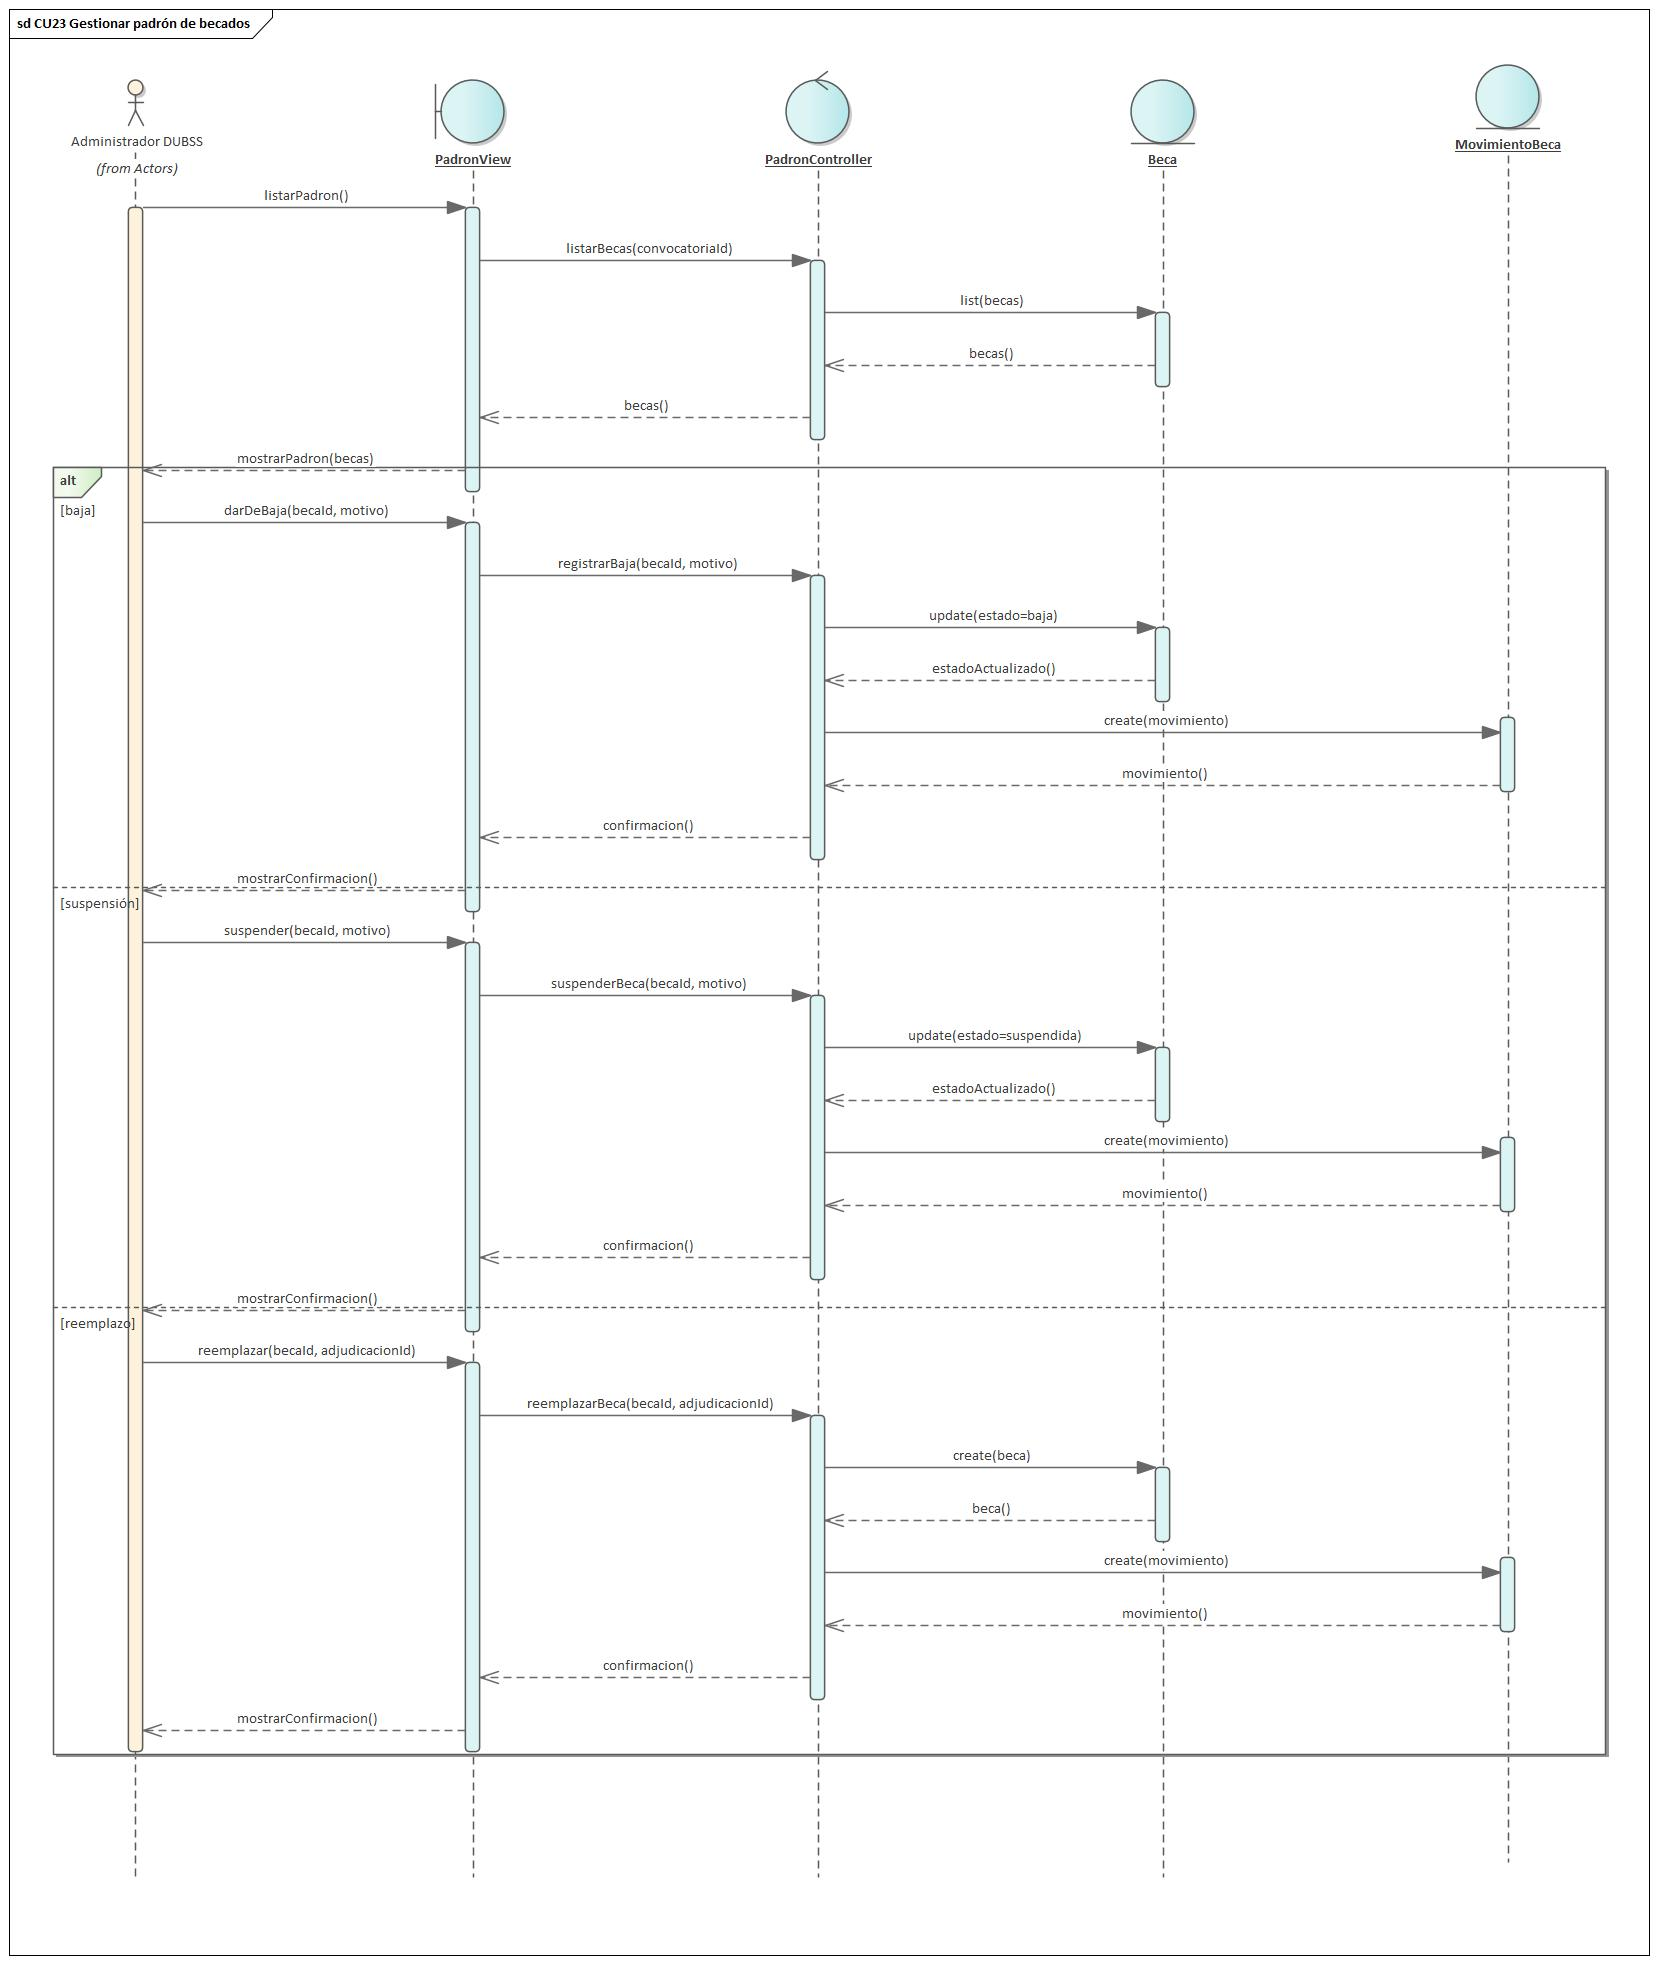
\includegraphics[width=\textwidth,height=0.75\textheight,keepaspectratio]{images/103_Secuencia_CU23_Gestionar_Padron_Becados.jpg}

\smallskip
\noindent\raggedright\textit{Nota.} Elaboración propia.
\end{figure}


\Needspace{0.9\textheight}
\subsubsection{7.4.24. Diseñar CU-24 Consultar historial de asistencia y estado de beca}\label{sec:cap7_disenar_cu24}

La Figura~\ref{fig:secuencia_cu24} presenta el diagrama de secuencia del CU-24.

\begin{figure}[H]
\caption{Diagrama de secuencia del CU-24 Consultar historial de asistencia y estado de beca}
\label{fig:secuencia_cu24}
\centering
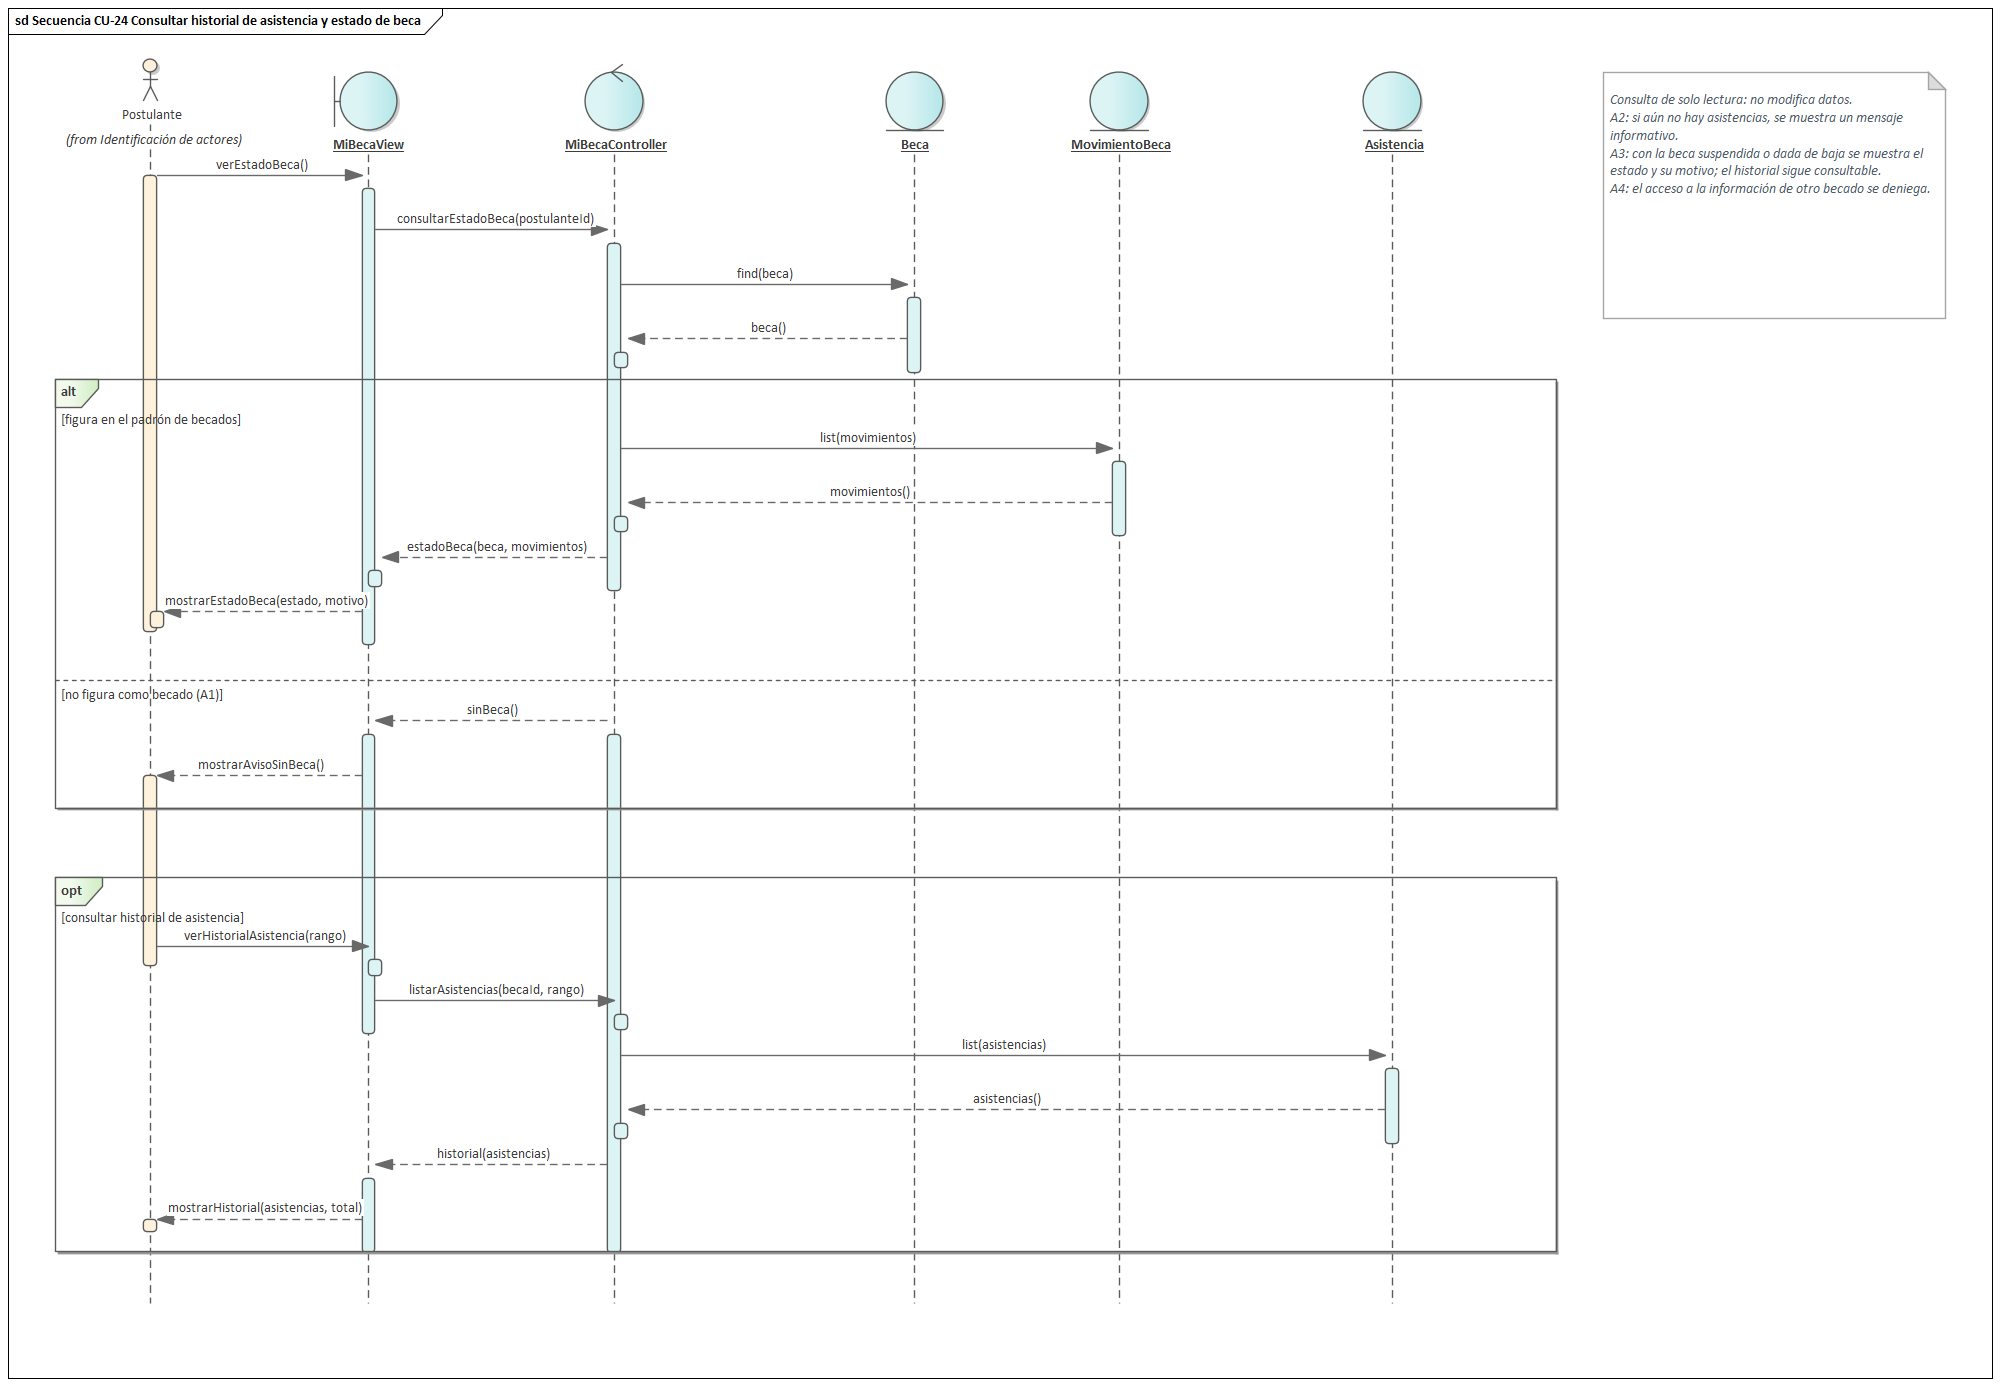
\includegraphics[width=\textwidth,height=0.75\textheight,keepaspectratio]{images/132_Secuencia_CU24_Consultar_Historial_Asistencia_Beca.png}

\smallskip
\noindent\raggedright\textit{Nota.} Elaboración propia.
\end{figure}


\Needspace{0.9\textheight}
\subsubsection{7.4.25. Diseñar CU-25 Consultar bitácora de acciones}\label{sec:cap7_disenar_cu25}

La Figura~\ref{fig:secuencia_cu25} presenta el diagrama de secuencia del CU-25.

\begin{figure}[H]
\caption{Diagrama de secuencia del CU-25 Consultar bitácora de acciones}
\label{fig:secuencia_cu25}
\centering
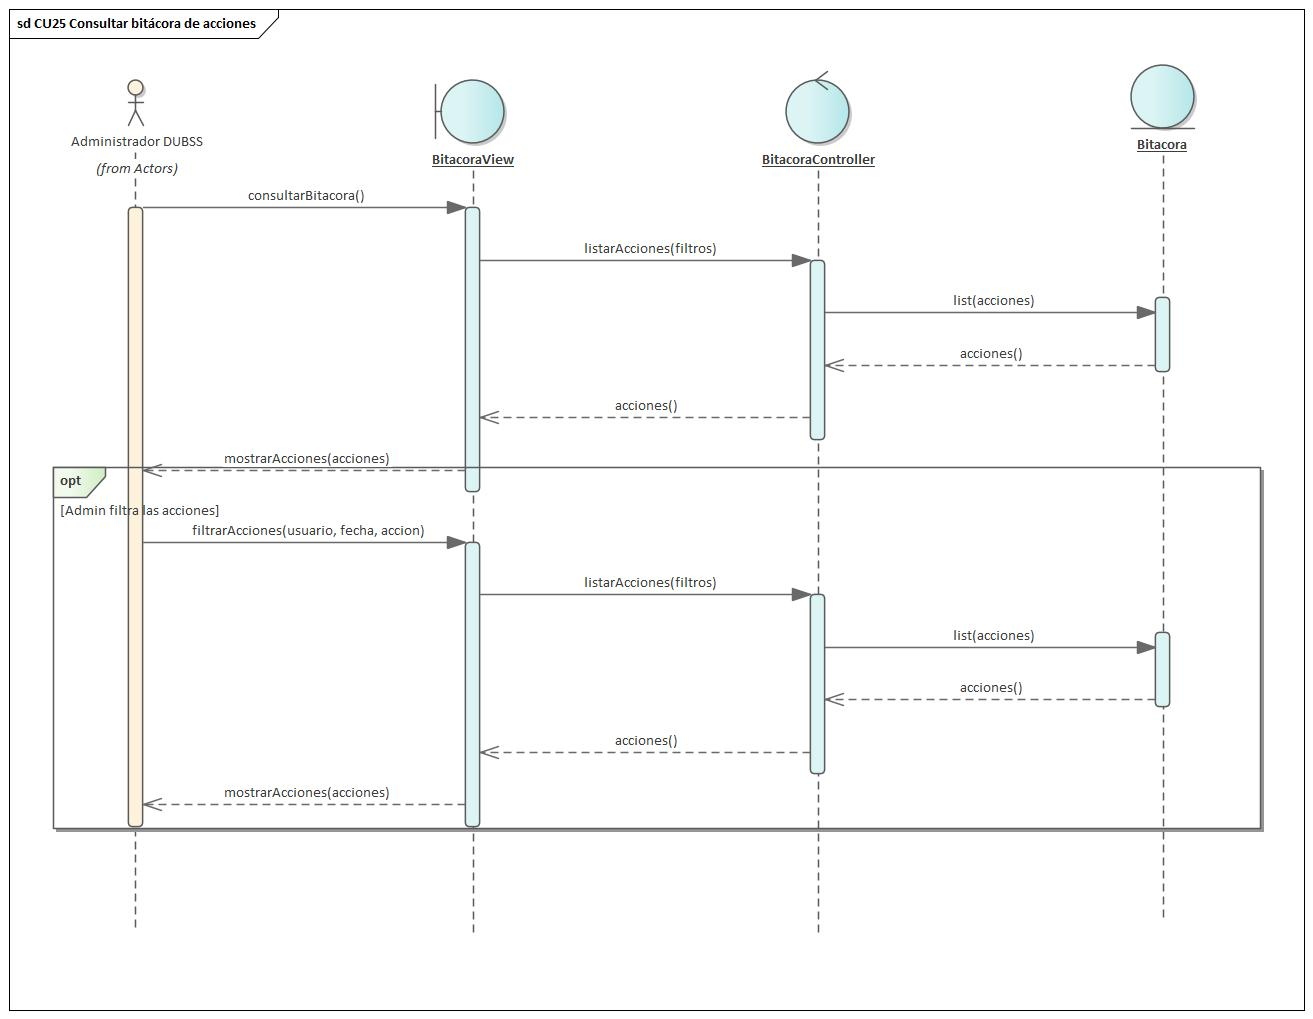
\includegraphics[width=\textwidth,height=0.75\textheight,keepaspectratio]{images/104_Secuencia_CU25_Consultar_Bitacora_Acciones.jpg}

\smallskip
\noindent\raggedright\textit{Nota.} Elaboración propia.
\end{figure}


\Needspace{0.9\textheight}
\subsubsection{7.4.26. Diseñar CU-26 Parametrizar modelo de preselección y reprocesar puntajes}\label{sec:cap7_disenar_cu26}

La Figura~\ref{fig:secuencia_cu26} presenta el diagrama de secuencia del CU-26.

\begin{figure}[H]
\caption{Diagrama de secuencia del CU-26 Parametrizar modelo de preselección y reprocesar puntajes}
\label{fig:secuencia_cu26}
\centering
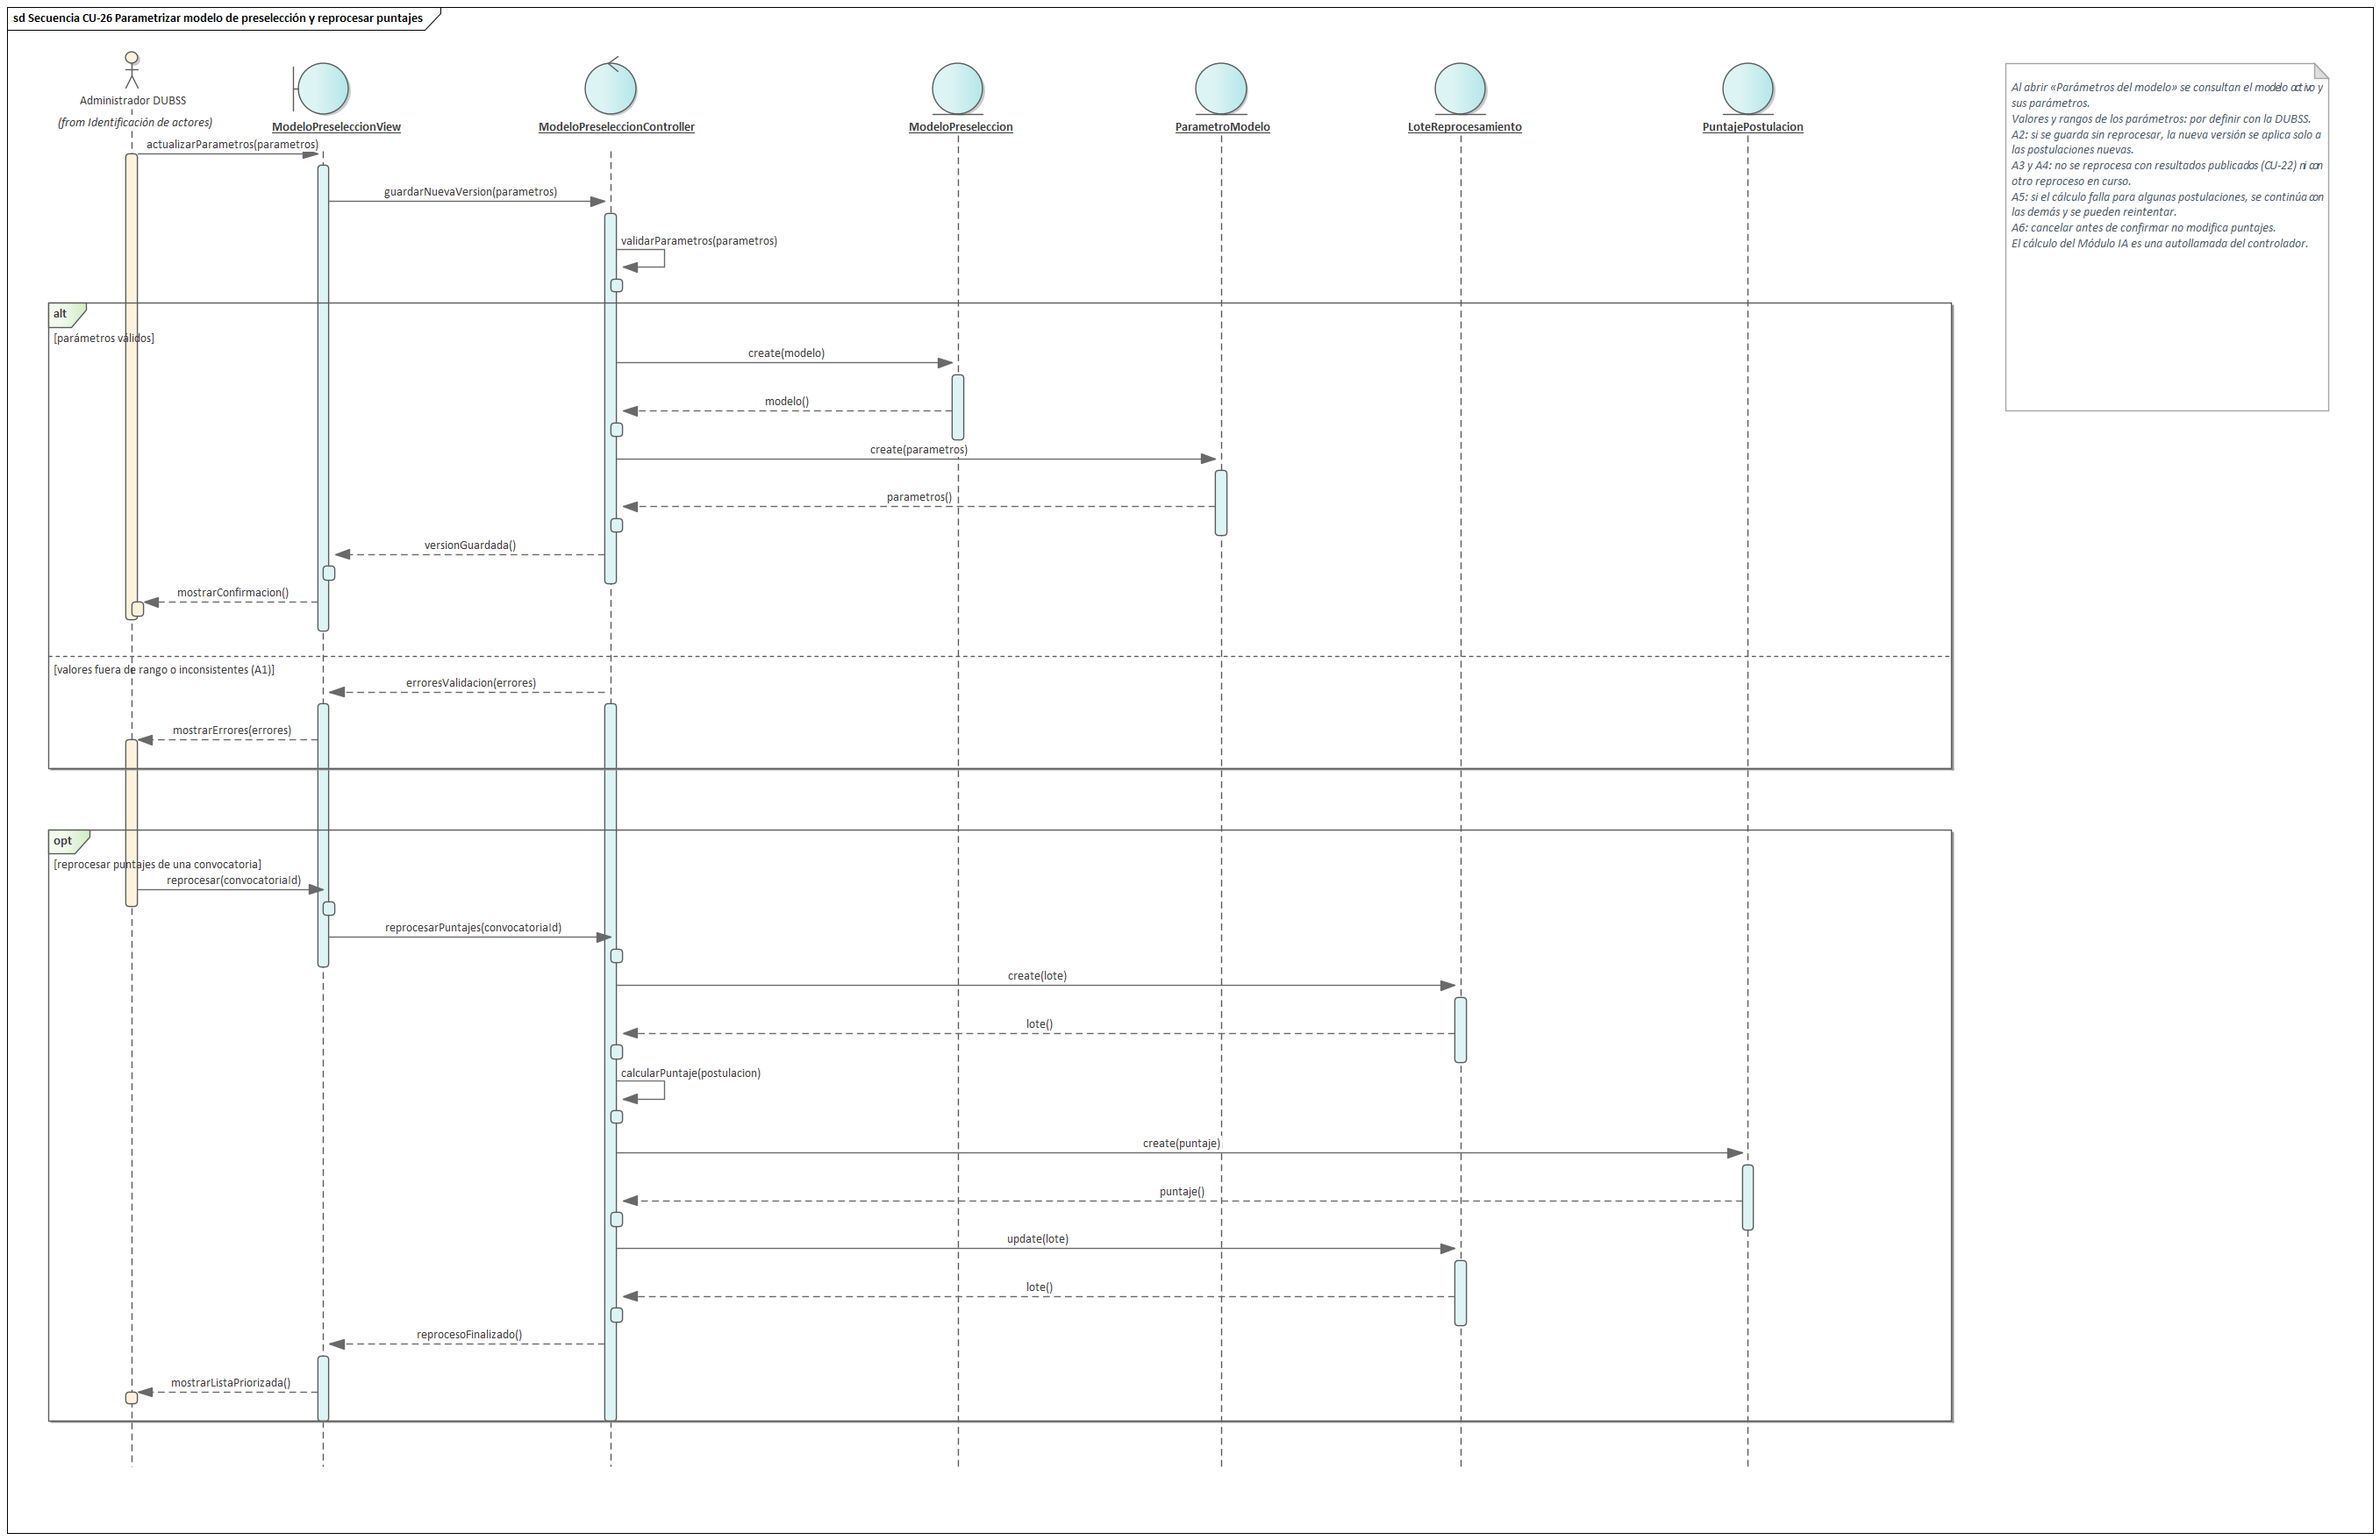
\includegraphics[width=\textwidth,height=0.75\textheight,keepaspectratio]{images/133_Secuencia_CU26_Parametrizar_Modelo_Preseleccion.png}

\smallskip
\noindent\raggedright\textit{Nota.} Elaboración propia.
\end{figure}


% ------------------------------------------------------------------------------
% 7.5. DISEÑO DE INTERFACES
% ------------------------------------------------------------------------------
\wfa{\wn{7}.5. Diseño de Interfaces}\label{sec:cap7_diseno_interfaces}

El diseño de interfaces expresa, mediante maquetas (\textit{mockups}), la disposición de los elementos visuales con los que el actor interactúa en cada caso de uso, de modo que las clases de interfaz (\textit{View}) identificadas en el análisis cuenten con una representación concreta \parencite{jacobson1999unified}.

A continuación se presenta el diseño de interfaces de los veintiséis casos de uso del sistema, en el orden de su numeración (CU-01 a CU-26).

\Needspace{0.9\textheight}
\wfb{\wn{7}.5.1. Interfaz CU-01 Registrarse y autenticarse}\label{sec:cap7_interfaz_cu01}

La Figura~\ref{fig:mockup_cu01} presenta la maqueta de interfaz del CU-01.

\begin{figure}[H]
\caption{Maqueta de interfaz del CU-01 Registrarse y autenticarse}
\label{fig:mockup_cu01}
\centering
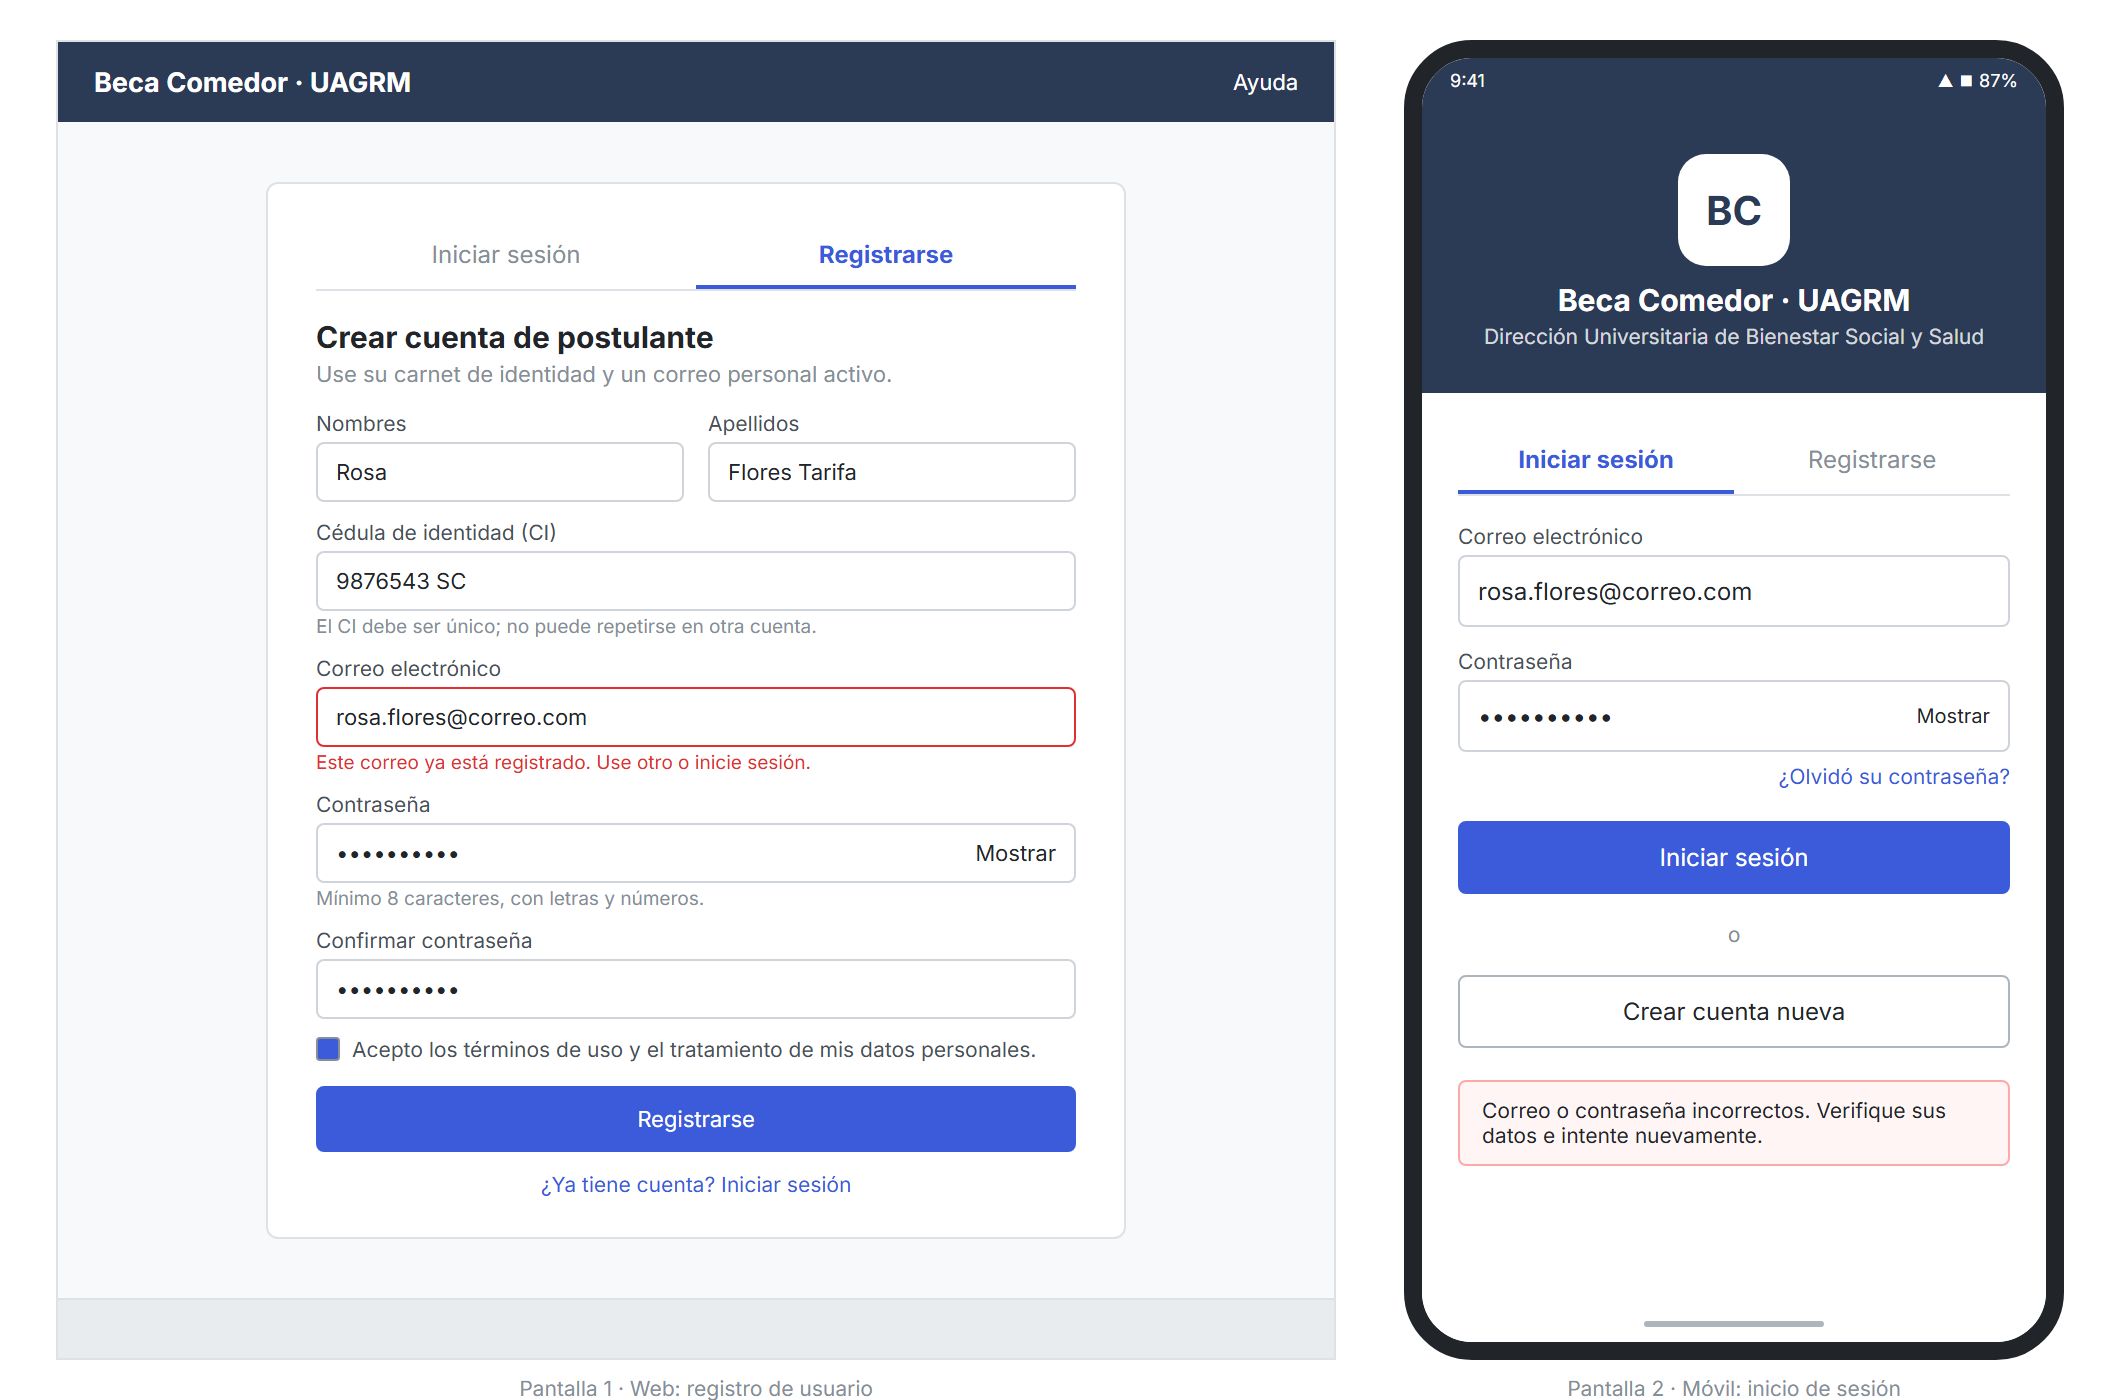
\includegraphics[width=\textwidth,height=0.75\textheight,keepaspectratio]{images/134_Mockup_CU01_Registrarse_autenticarse.png}

\smallskip
\noindent\raggedright\textit{Nota.} Elaboración propia.
\end{figure}



\Needspace{0.9\textheight}
\wfb{\wn{7}.5.2. Interfaz CU-02 Enviar postulación a Beca Comedor}\label{sec:cap7_interfaz_cu02}

La Figura~\ref{fig:mockup_cu02} presenta la maqueta de interfaz del CU-02.

\begin{figure}[H]
\caption{Maqueta de interfaz del CU-02 Enviar postulación a Beca Comedor}
\label{fig:mockup_cu02}
\centering
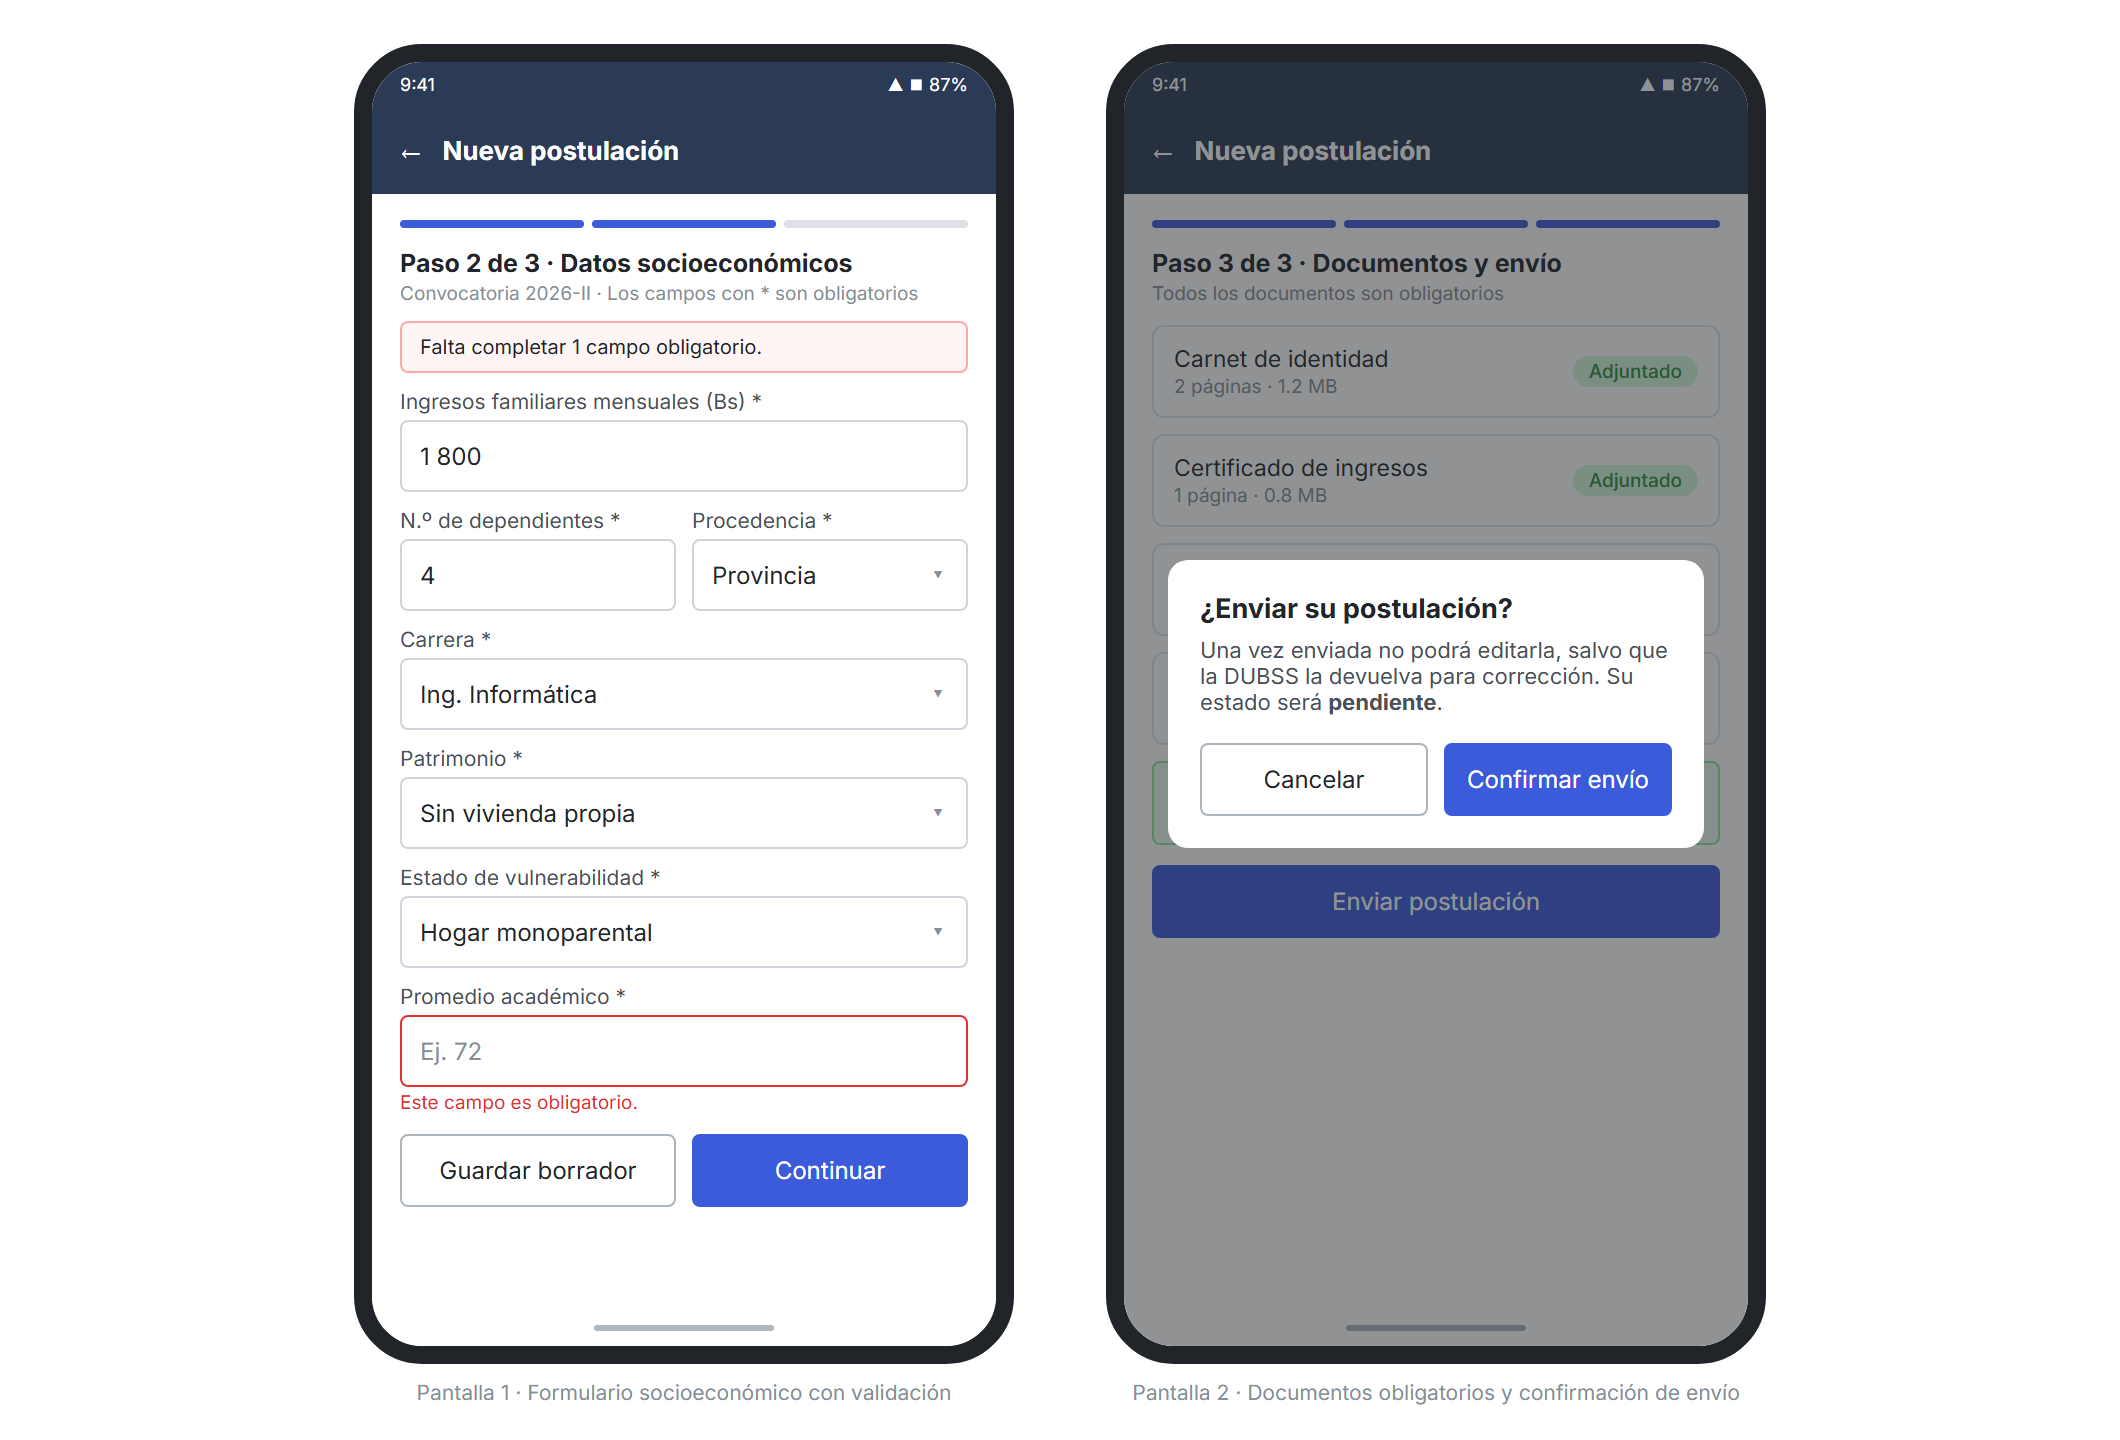
\includegraphics[width=\textwidth,height=0.75\textheight,keepaspectratio]{images/135_Mockup_CU02_Enviar_postulacion.png}

\smallskip
\noindent\raggedright\textit{Nota.} Elaboración propia.
\end{figure}



\Needspace{0.9\textheight}
\wfb{\wn{7}.5.3. Interfaz CU-03 Precalificar postulación con Inteligencia Artificial}\label{sec:cap7_interfaz_cu03}

La Figura~\ref{fig:mockup_cu03} presenta la maqueta de interfaz del CU-03.

\begin{figure}[H]
\caption{Maqueta de interfaz del CU-03 Precalificar postulación con Inteligencia Artificial}
\label{fig:mockup_cu03}
\centering
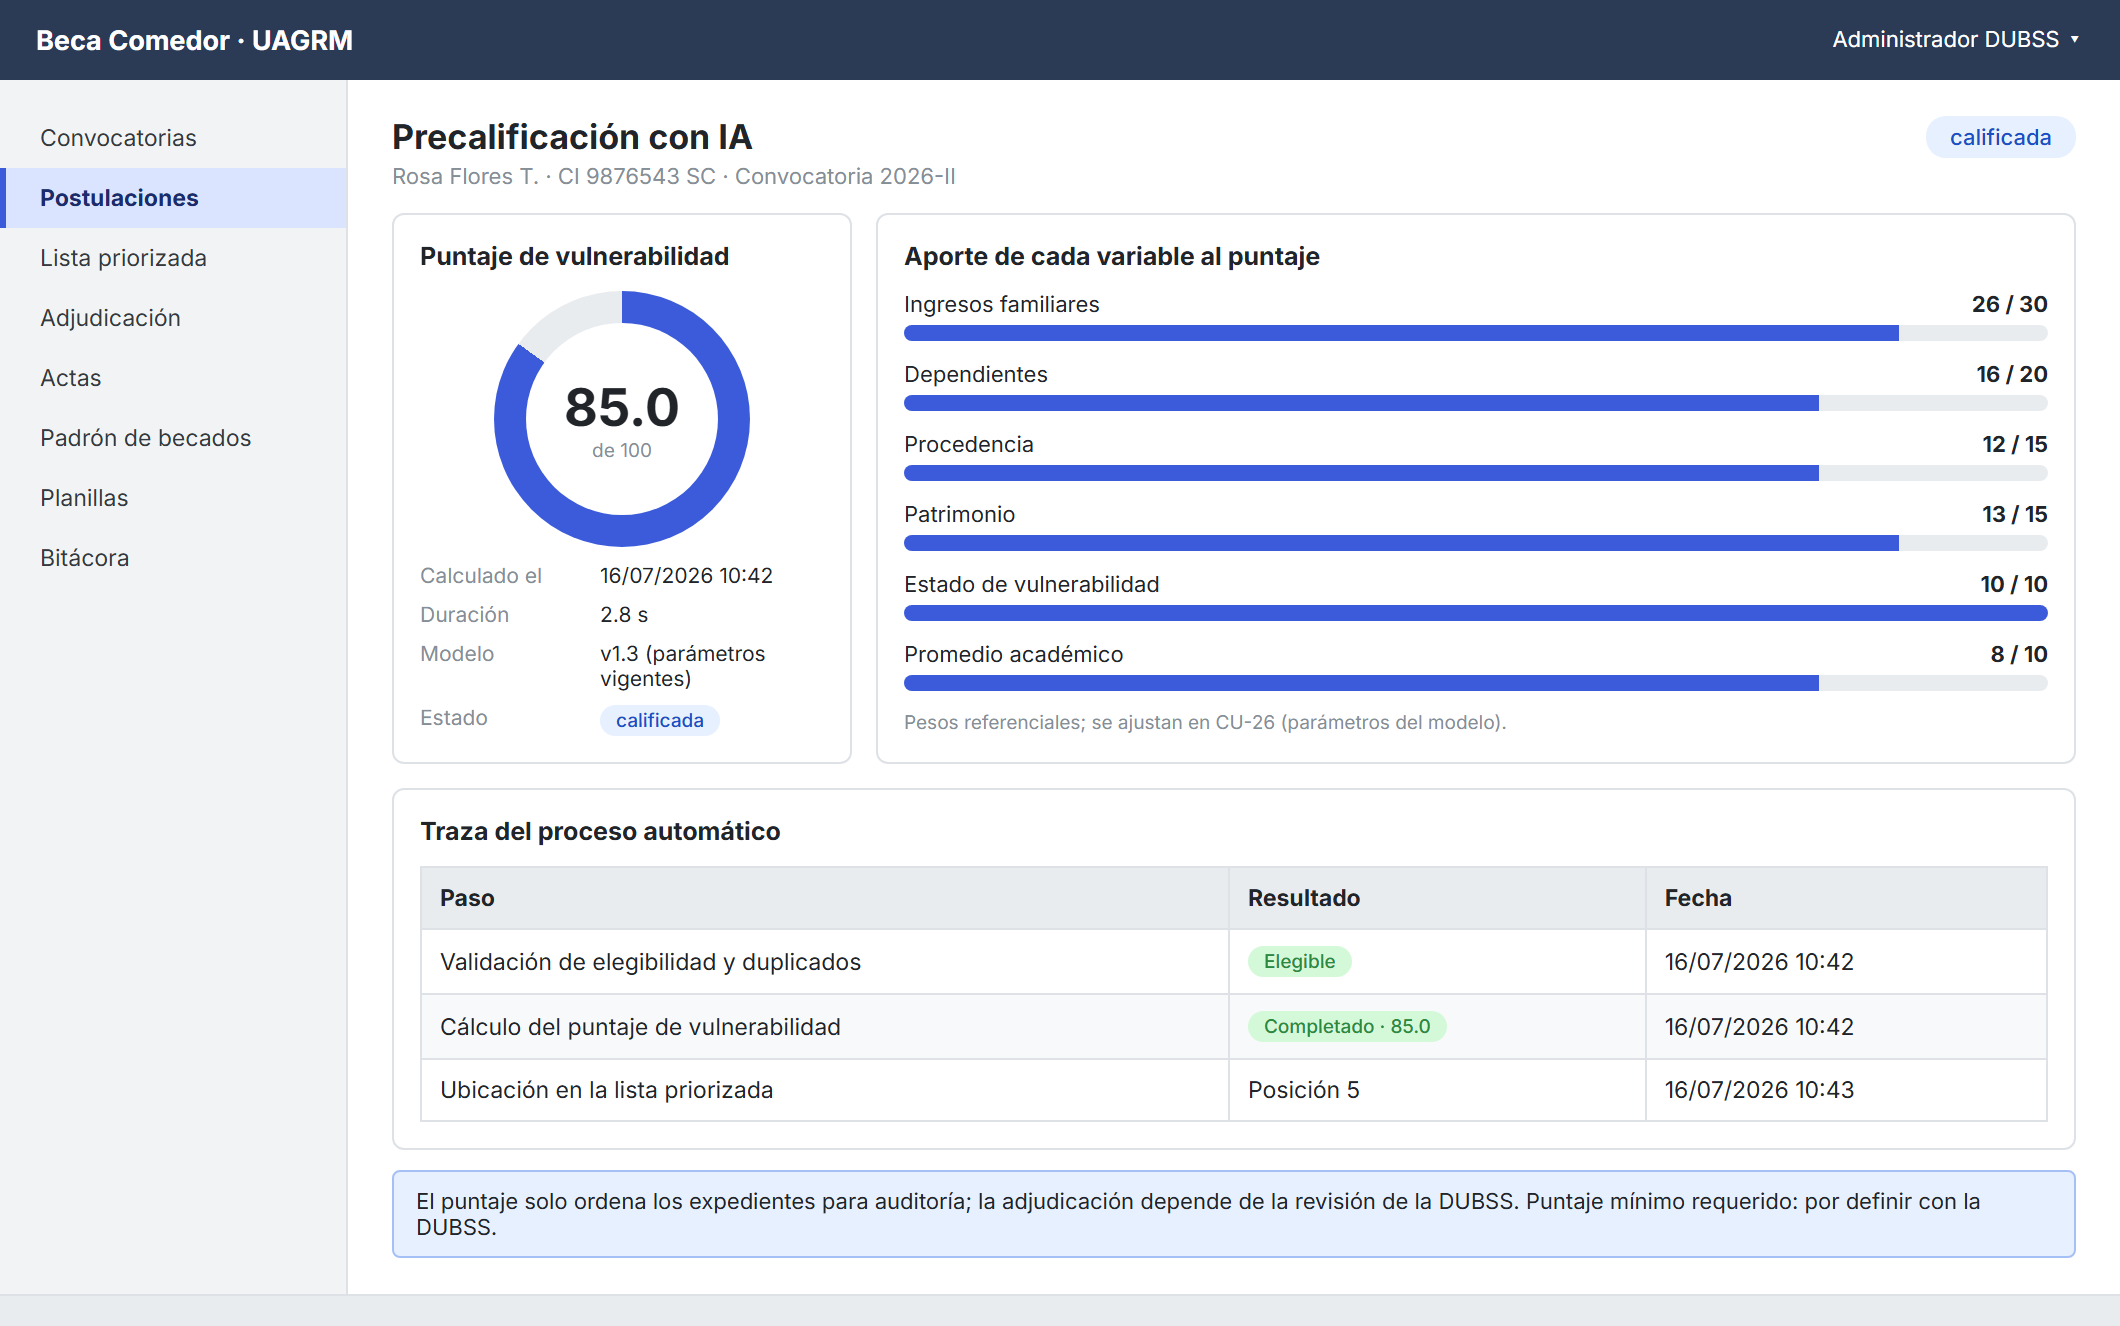
\includegraphics[width=\textwidth,height=0.75\textheight,keepaspectratio]{images/136_Mockup_CU03_Precalificar_IA.png}

\smallskip
\noindent\raggedright\textit{Nota.} Elaboración propia.
\end{figure}



\Needspace{0.9\textheight}
\wfb{\wn{7}.5.4. Interfaz CU-04 Consultar estado de postulación}\label{sec:cap7_interfaz_cu04}

La Figura~\ref{fig:mockup_cu04} presenta la maqueta de interfaz del CU-04.

\begin{figure}[H]
\caption{Maqueta de interfaz del CU-04 Consultar estado de postulación}
\label{fig:mockup_cu04}
\centering
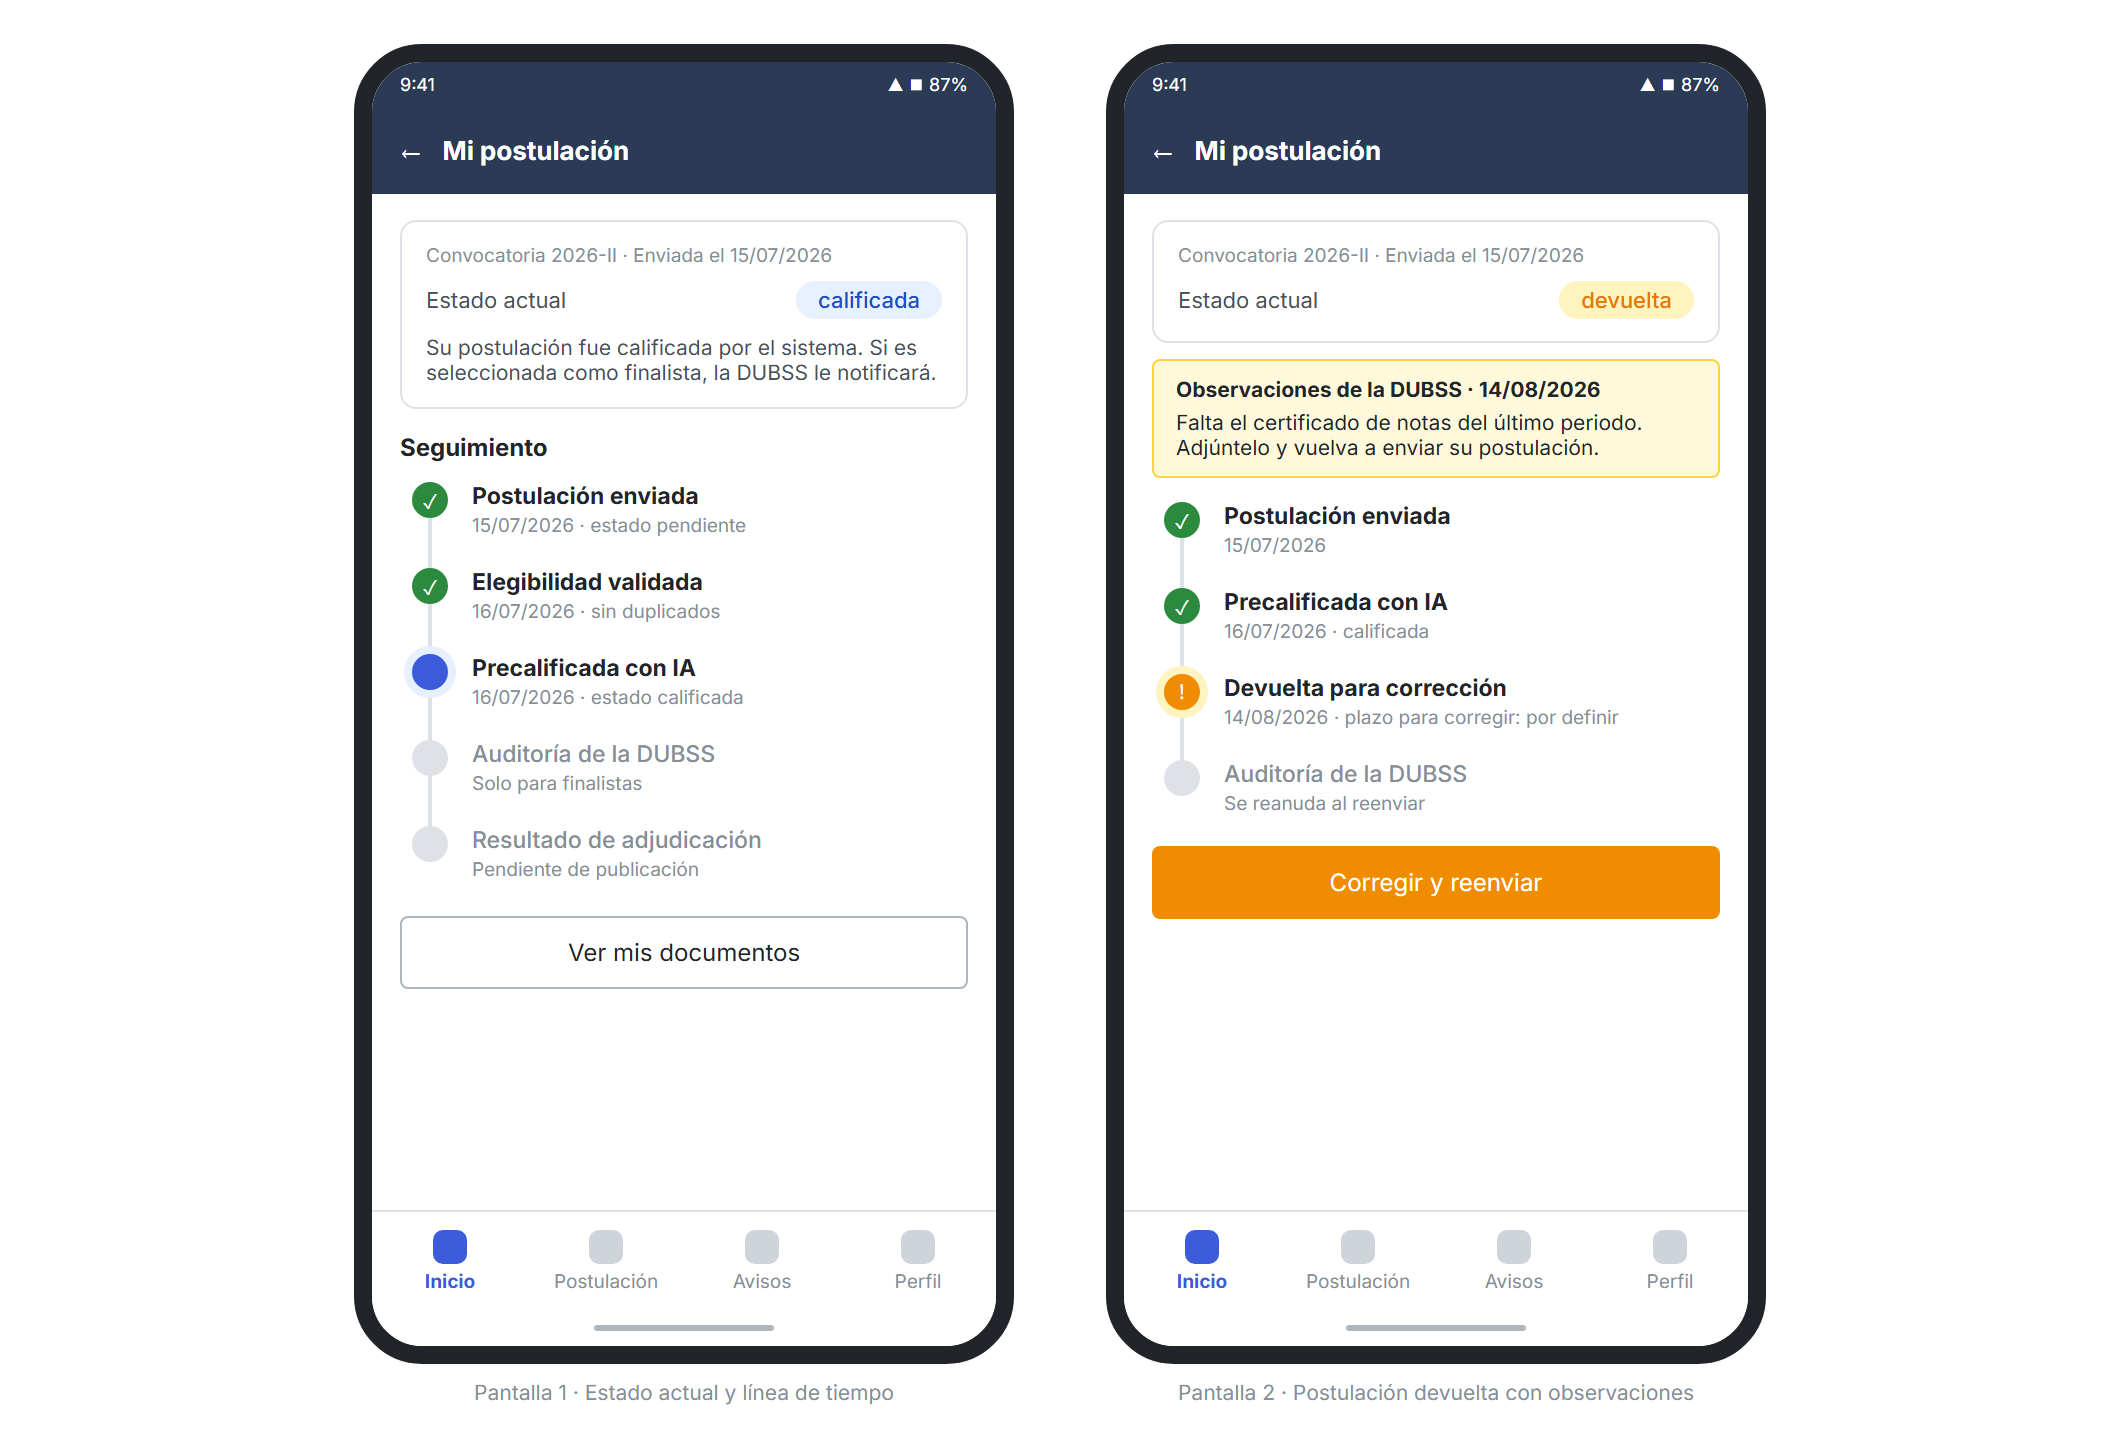
\includegraphics[width=\textwidth,height=0.75\textheight,keepaspectratio]{images/137_Mockup_CU04_Consultar_estado.png}

\smallskip
\noindent\raggedright\textit{Nota.} Elaboración propia.
\end{figure}



\Needspace{0.9\textheight}
\wfb{\wn{7}.5.5. Interfaz CU-05 Auditar y adjudicar becas}\label{sec:cap7_interfaz_cu05}

La Figura~\ref{fig:mockup_cu05} presenta la maqueta de interfaz del CU-05.

\begin{figure}[H]
\caption{Maqueta de interfaz del CU-05 Auditar y adjudicar becas}
\label{fig:mockup_cu05}
\centering
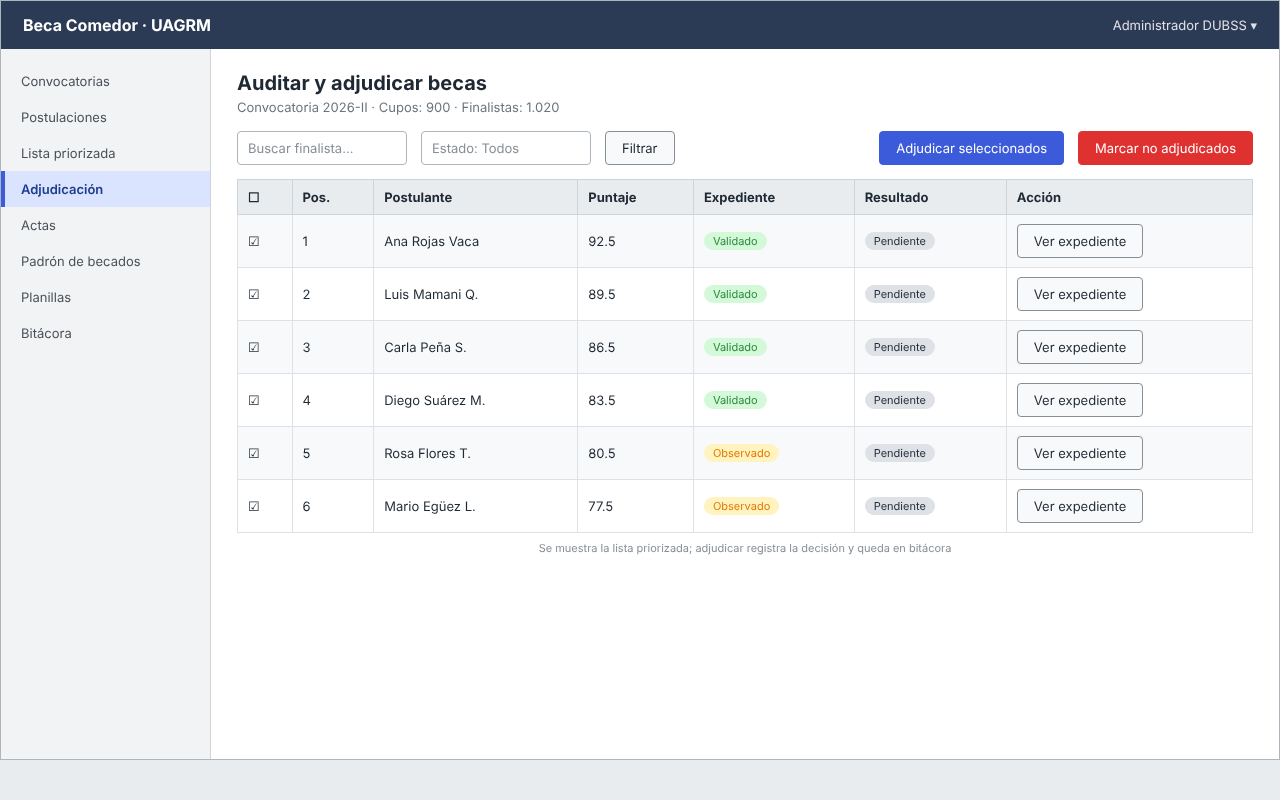
\includegraphics[width=\textwidth,height=0.75\textheight,keepaspectratio]{images/105_Mockup_CU05_Auditar_y_adjudicar_becas.png}

\smallskip
\noindent\raggedright\textit{Nota.} Elaboración propia.
\end{figure}


\Needspace{0.9\textheight}
\wfb{\wn{7}.5.6. Interfaz CU-06 Visualizar lista priorizada de postulantes}\label{sec:cap7_interfaz_cu06}

La Figura~\ref{fig:mockup_cu06} presenta la maqueta de interfaz del CU-06.

\begin{figure}[H]
\caption{Maqueta de interfaz del CU-06 Visualizar lista priorizada de postulantes}
\label{fig:mockup_cu06}
\centering
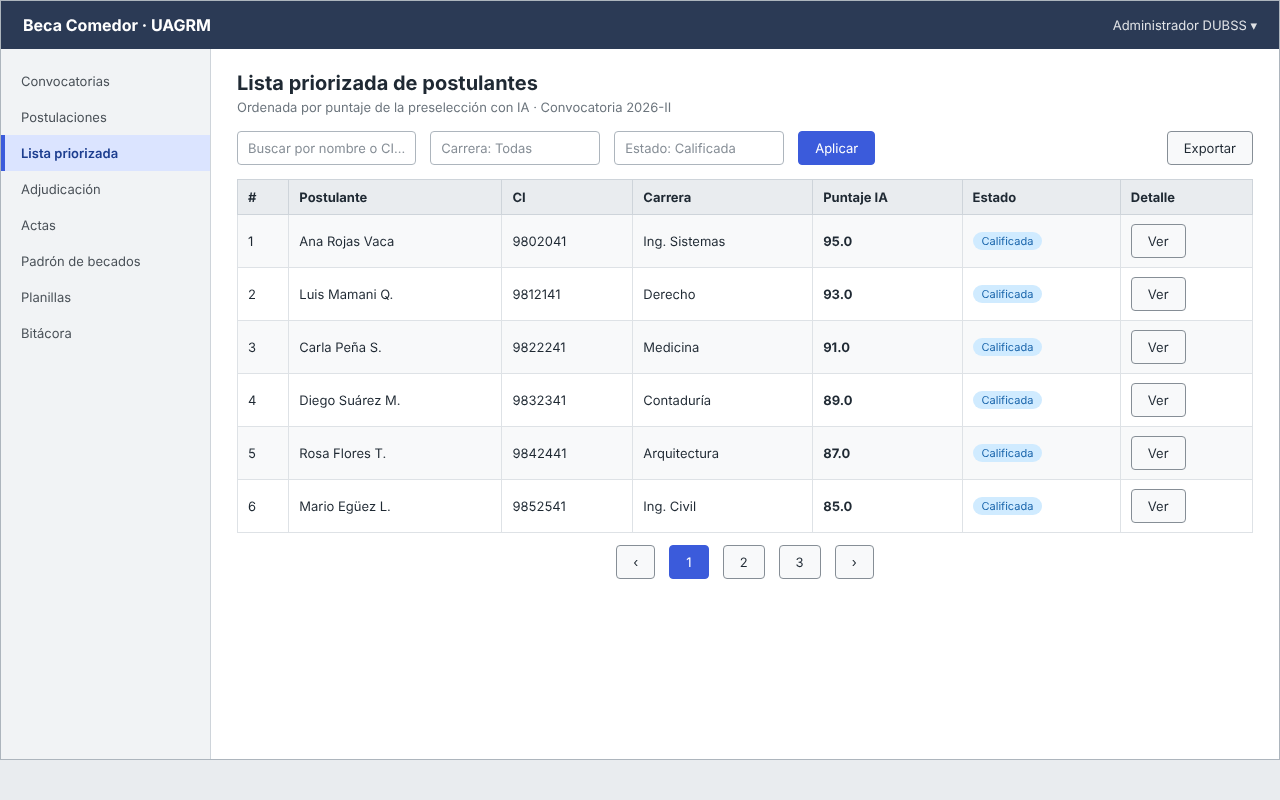
\includegraphics[width=\textwidth,height=0.75\textheight,keepaspectratio]{images/106_Mockup_CU06_Lista_priorizada.png}

\smallskip
\noindent\raggedright\textit{Nota.} Elaboración propia.
\end{figure}


\Needspace{0.9\textheight}
\wfb{\wn{7}.5.7. Interfaz CU-07 Auditar expediente finalista}\label{sec:cap7_interfaz_cu07}

La Figura~\ref{fig:mockup_cu07} presenta la maqueta de interfaz del CU-07.

\begin{figure}[H]
\caption{Maqueta de interfaz del CU-07 Auditar expediente finalista}
\label{fig:mockup_cu07}
\centering
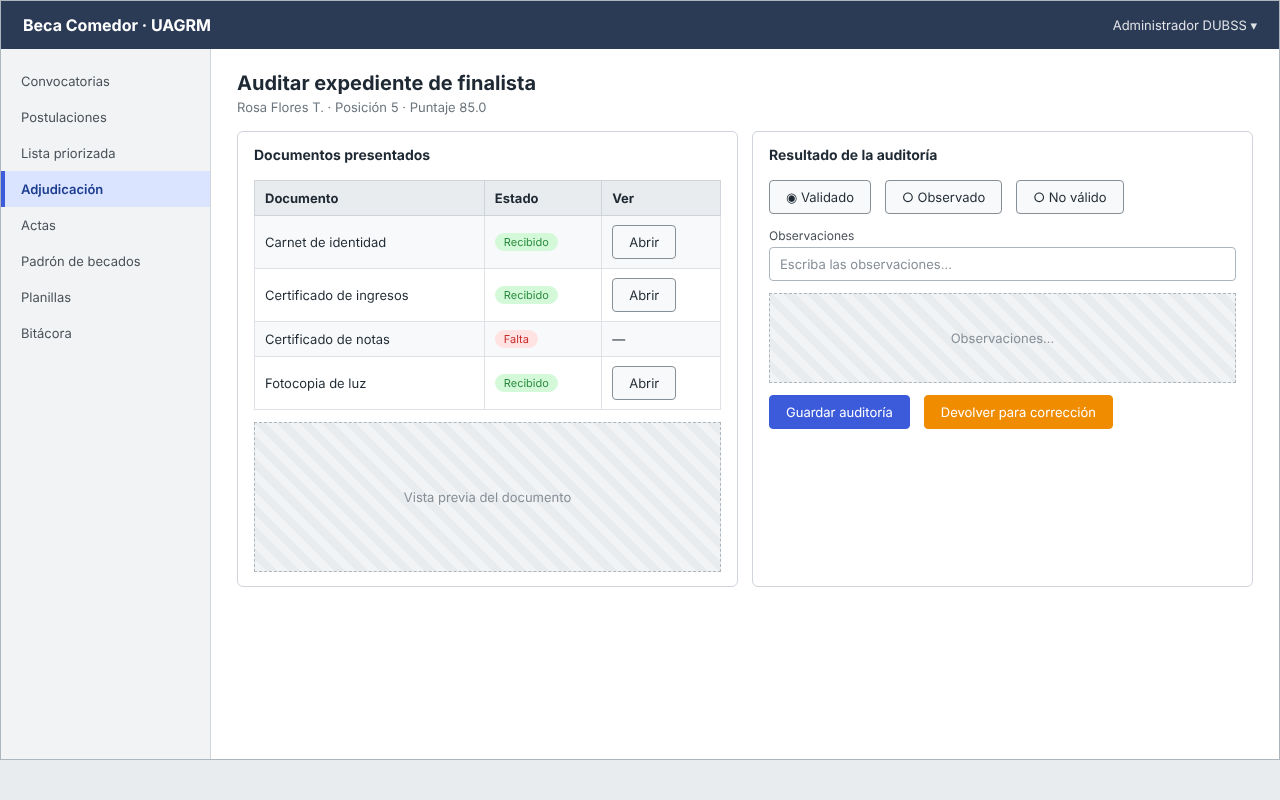
\includegraphics[width=\textwidth,height=0.75\textheight,keepaspectratio]{images/107_Mockup_CU07_Auditar_expediente_finalista.png}

\smallskip
\noindent\raggedright\textit{Nota.} Elaboración propia.
\end{figure}


\Needspace{0.9\textheight}
\wfb{\wn{7}.5.8. Interfaz CU-08 Generar acta de adjudicación}\label{sec:cap7_interfaz_cu08}

La Figura~\ref{fig:mockup_cu08} presenta la maqueta de interfaz del CU-08.

\begin{figure}[H]
\caption{Maqueta de interfaz del CU-08 Generar acta de adjudicación}
\label{fig:mockup_cu08}
\centering
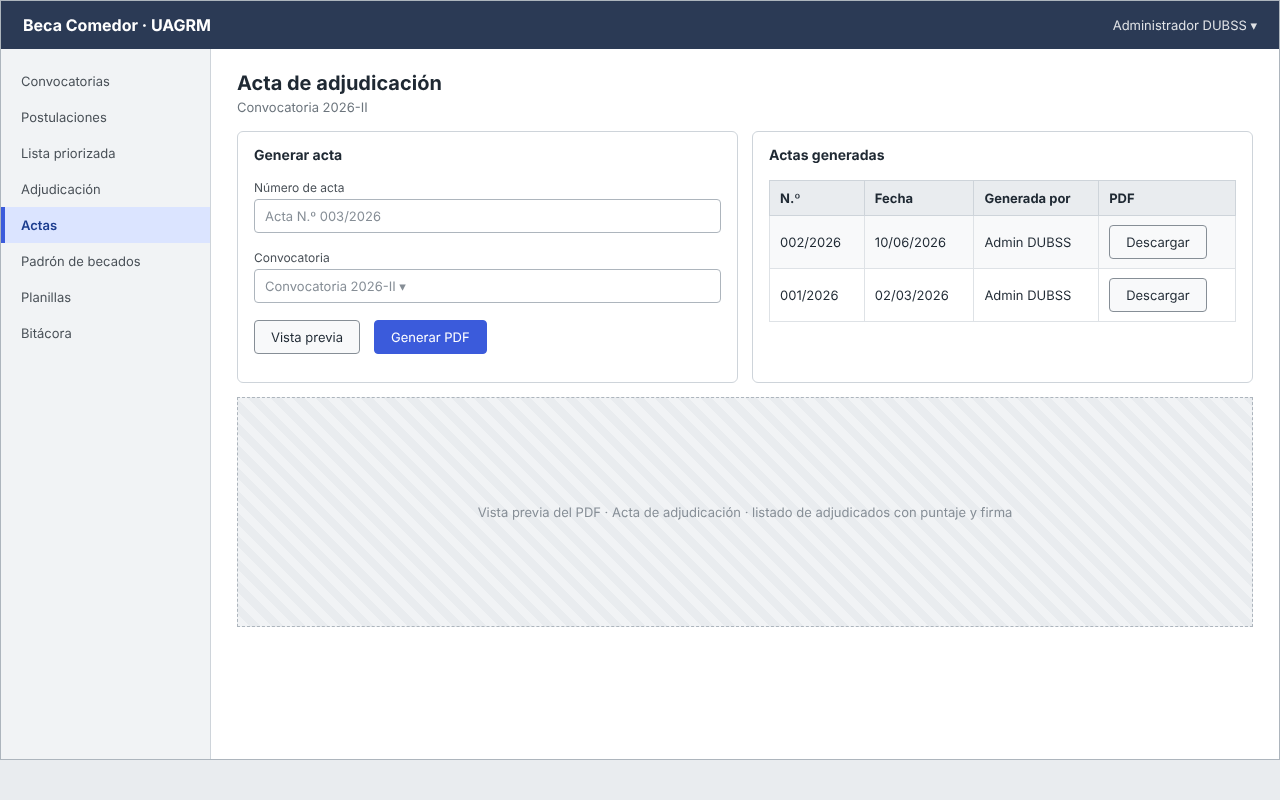
\includegraphics[width=\textwidth,height=0.75\textheight,keepaspectratio]{images/108_Mockup_CU08_Acta_de_adjudicacion.png}

\smallskip
\noindent\raggedright\textit{Nota.} Elaboración propia.
\end{figure}


\Needspace{0.9\textheight}
\wfb{\wn{7}.5.9. Interfaz CU-09 Generar planilla de asistencia}\label{sec:cap7_interfaz_cu09}

La Figura~\ref{fig:mockup_cu09} presenta la maqueta de interfaz del CU-09.

\begin{figure}[H]
\caption{Maqueta de interfaz del CU-09 Generar planilla de asistencia}
\label{fig:mockup_cu09}
\centering
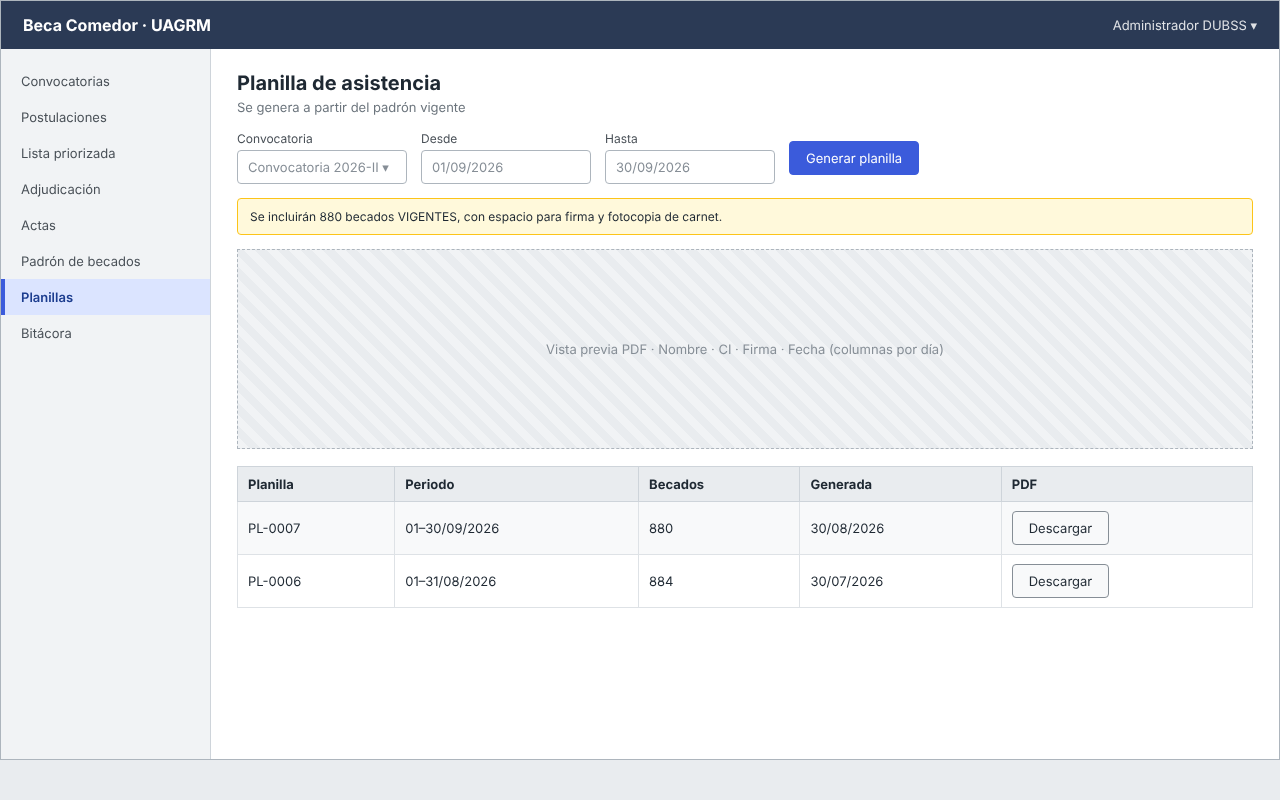
\includegraphics[width=\textwidth,height=0.75\textheight,keepaspectratio]{images/109_Mockup_CU09_Planilla_de_asistencia.png}

\smallskip
\noindent\raggedright\textit{Nota.} Elaboración propia.
\end{figure}


\Needspace{0.9\textheight}
\wfb{\wn{7}.5.10. Interfaz CU-10 Registrar asistencia digital}\label{sec:cap7_interfaz_cu10}

La Figura~\ref{fig:mockup_cu10} presenta la maqueta de interfaz del CU-10.

\begin{figure}[H]
\caption{Maqueta de interfaz del CU-10 Registrar asistencia digital}
\label{fig:mockup_cu10}
\centering
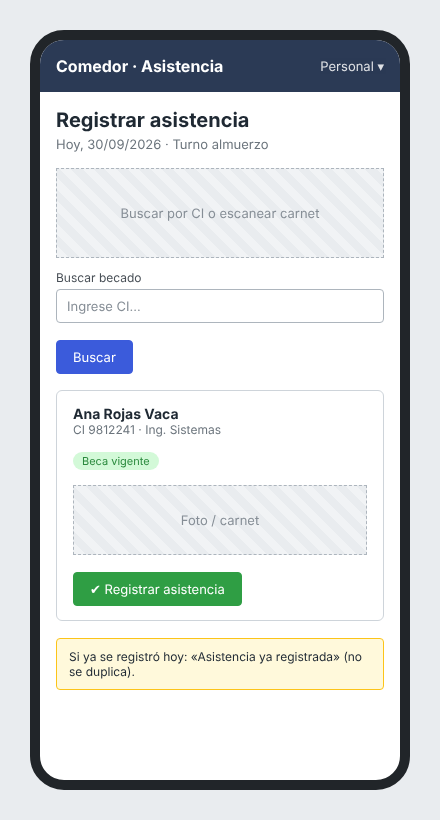
\includegraphics[width=\textwidth,height=0.75\textheight,keepaspectratio]{images/110_Mockup_CU10_Registrar_asistencia_digital.png}

\smallskip
\noindent\raggedright\textit{Nota.} Elaboración propia.
\end{figure}


\Needspace{0.9\textheight}
\wfb{\wn{7}.5.11. Interfaz CU-11 Cotejar registro contra respaldo físico}\label{sec:cap7_interfaz_cu11}

La Figura~\ref{fig:mockup_cu11} presenta la maqueta de interfaz del CU-11.

\begin{figure}[H]
\caption{Maqueta de interfaz del CU-11 Cotejar registro contra respaldo físico}
\label{fig:mockup_cu11}
\centering
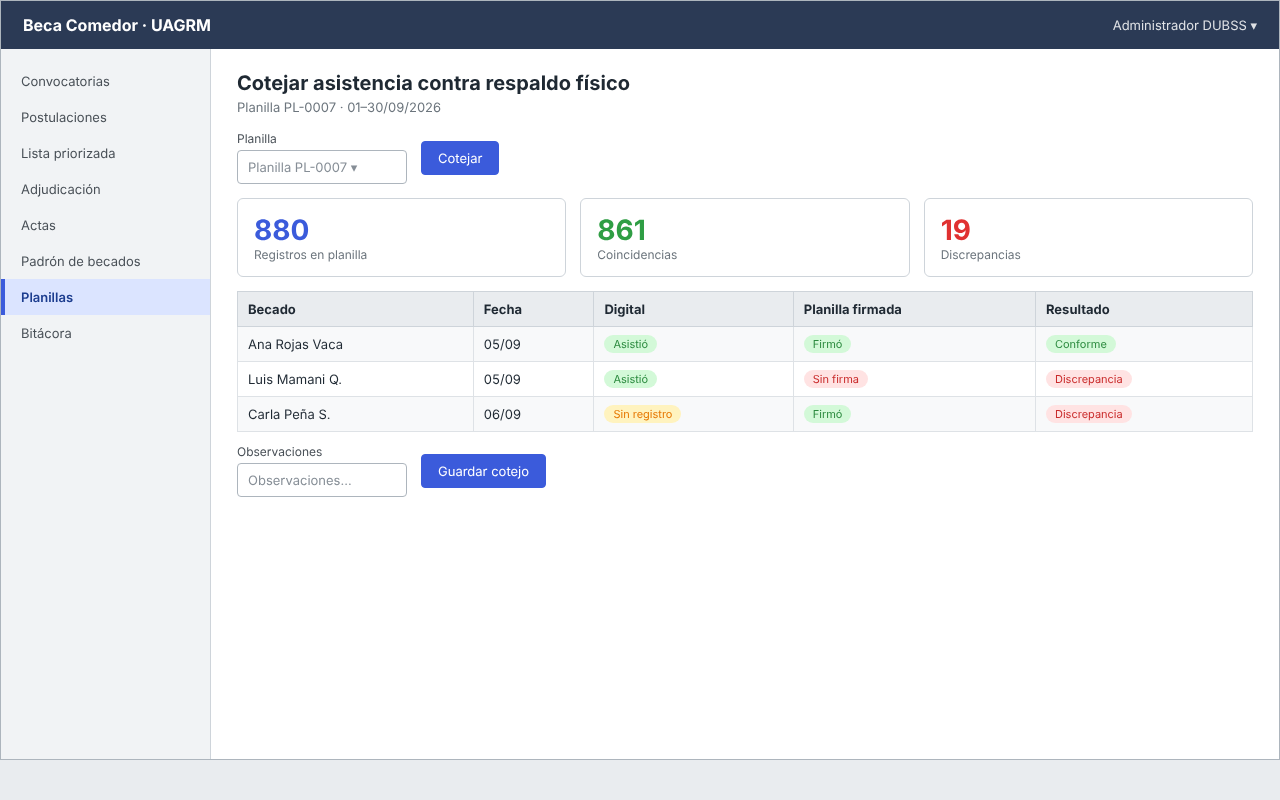
\includegraphics[width=\textwidth,height=0.75\textheight,keepaspectratio]{images/111_Mockup_CU11_Cotejar_contra_respaldo_fisico.png}

\smallskip
\noindent\raggedright\textit{Nota.} Elaboración propia.
\end{figure}


\Needspace{0.9\textheight}
\wfb{\wn{7}.5.12. Interfaz CU-12 Visualizar dashboard de indicadores BI}\label{sec:cap7_interfaz_cu12}

La Figura~\ref{fig:mockup_cu12} presenta la maqueta de interfaz del CU-12.

\begin{figure}[H]
\caption{Maqueta de interfaz del CU-12 Visualizar dashboard de indicadores BI}
\label{fig:mockup_cu12}
\centering
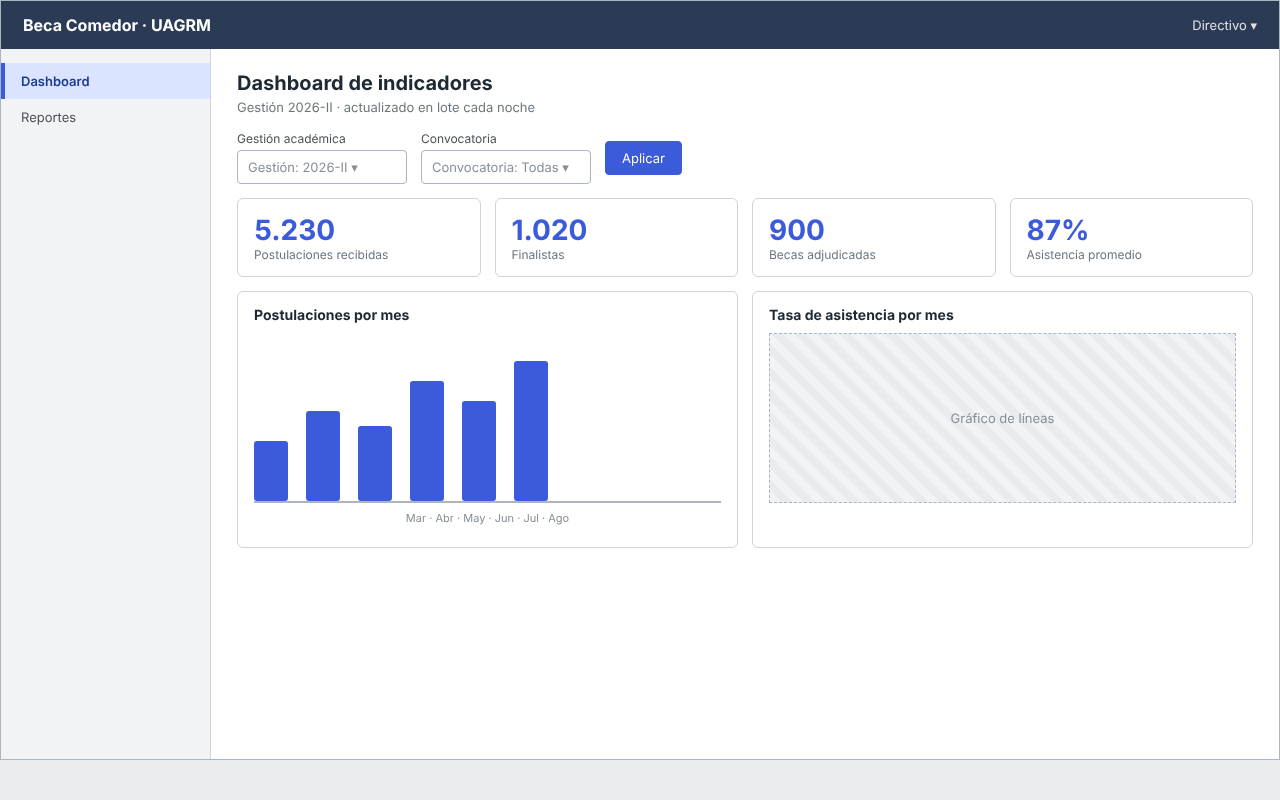
\includegraphics[width=\textwidth,height=0.75\textheight,keepaspectratio]{images/112_Mockup_CU12_Dashboard_BI.png}

\smallskip
\noindent\raggedright\textit{Nota.} Elaboración propia.
\end{figure}


\Needspace{0.9\textheight}
\wfb{\wn{7}.5.13. Interfaz CU-13 Gestionar convocatoria y gestión académica}\label{sec:cap7_interfaz_cu13}

La Figura~\ref{fig:mockup_cu13} presenta la maqueta de interfaz del CU-13.

\begin{figure}[H]
\caption{Maqueta de interfaz del CU-13 Gestionar convocatoria y gestión académica}
\label{fig:mockup_cu13}
\centering
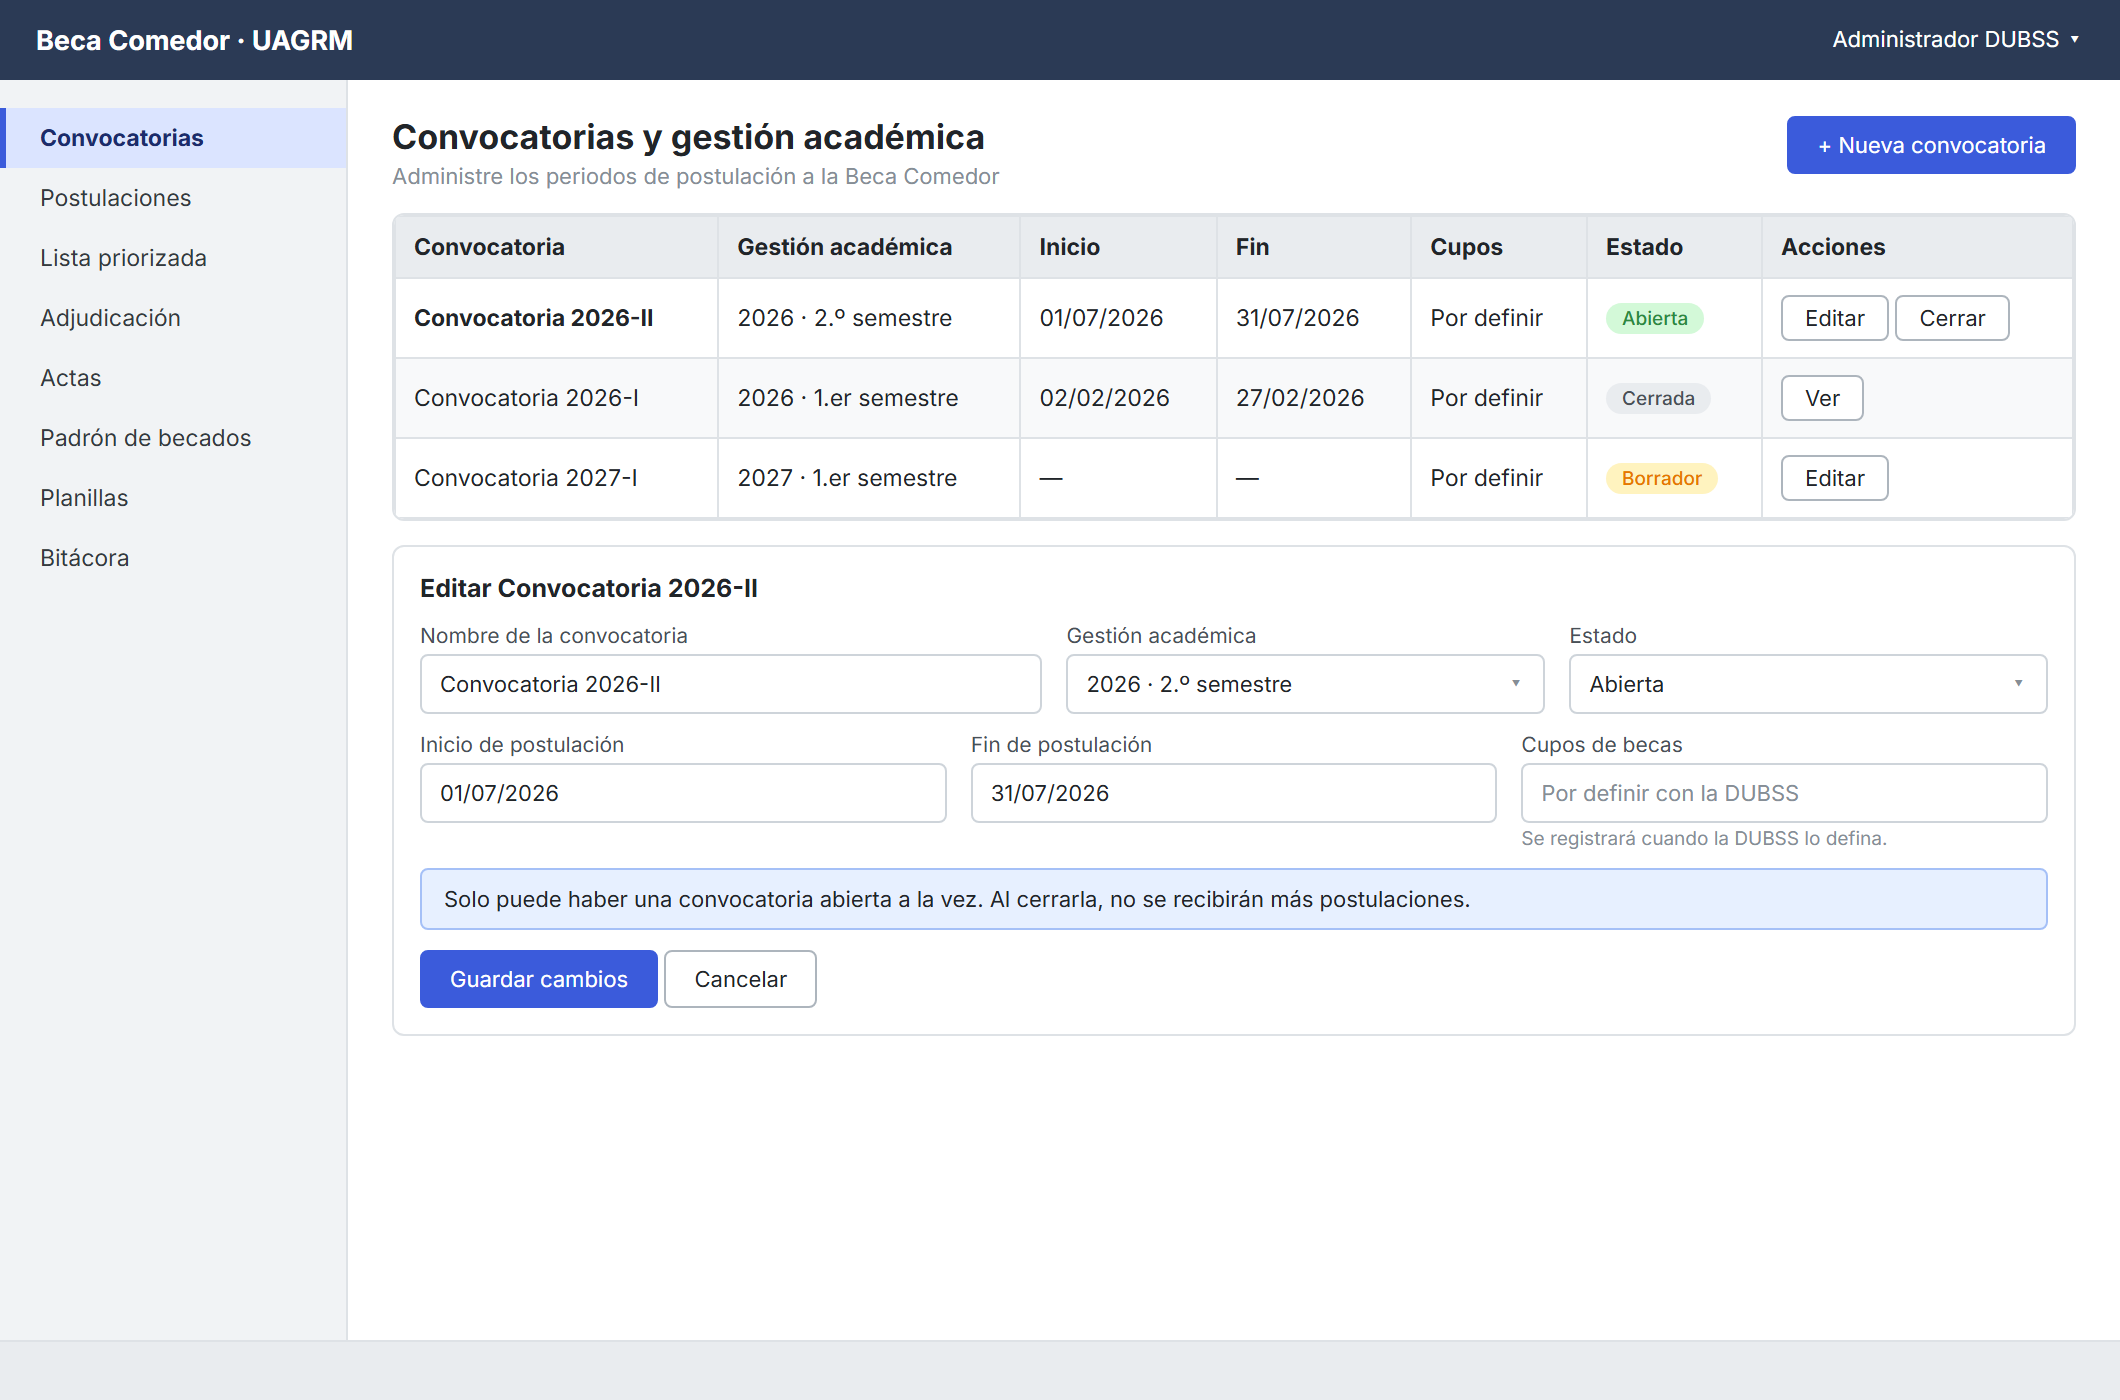
\includegraphics[width=\textwidth,height=0.75\textheight,keepaspectratio]{images/138_Mockup_CU13_Gestionar_convocatoria.png}

\smallskip
\noindent\raggedright\textit{Nota.} Elaboración propia.
\end{figure}



\Needspace{0.9\textheight}
\wfb{\wn{7}.5.14. Interfaz CU-14 Gestionar usuarios y roles}\label{sec:cap7_interfaz_cu14}

La Figura~\ref{fig:mockup_cu14} presenta la maqueta de interfaz del CU-14.

\begin{figure}[H]
\caption{Maqueta de interfaz del CU-14 Gestionar usuarios y roles}
\label{fig:mockup_cu14}
\centering
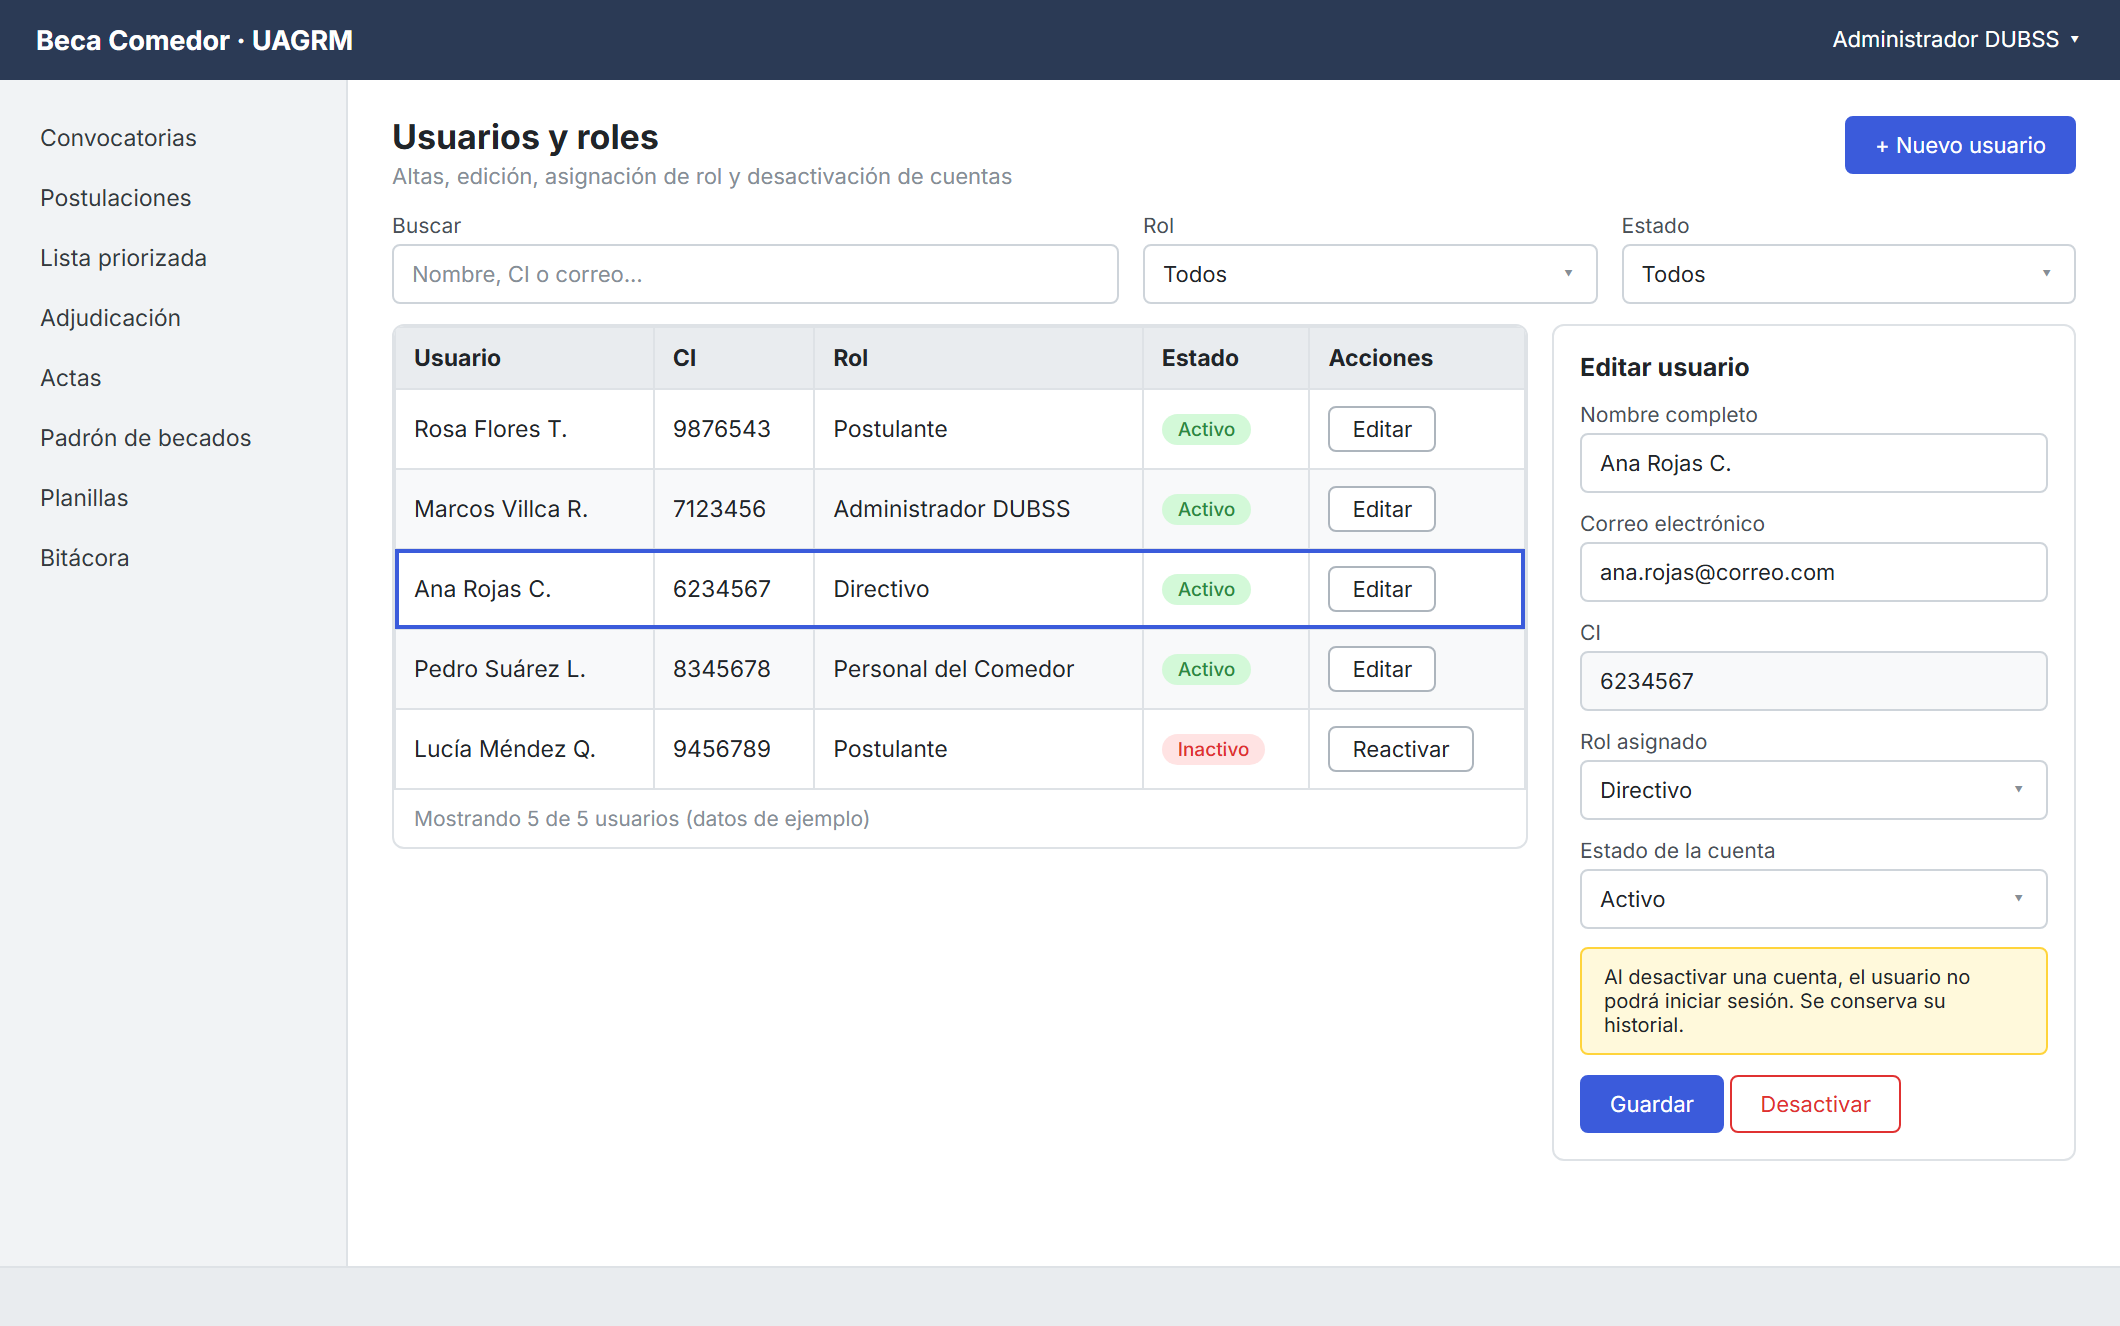
\includegraphics[width=\textwidth,height=0.75\textheight,keepaspectratio]{images/139_Mockup_CU14_Gestionar_usuarios_roles.png}

\smallskip
\noindent\raggedright\textit{Nota.} Elaboración propia.
\end{figure}



\Needspace{0.9\textheight}
\wfb{\wn{7}.5.15. Interfaz CU-15 Recuperar contraseña / gestionar perfil}\label{sec:cap7_interfaz_cu15}

La Figura~\ref{fig:mockup_cu15} presenta la maqueta de interfaz del CU-15.

\begin{figure}[H]
\caption{Maqueta de interfaz del CU-15 Recuperar contraseña / gestionar perfil}
\label{fig:mockup_cu15}
\centering
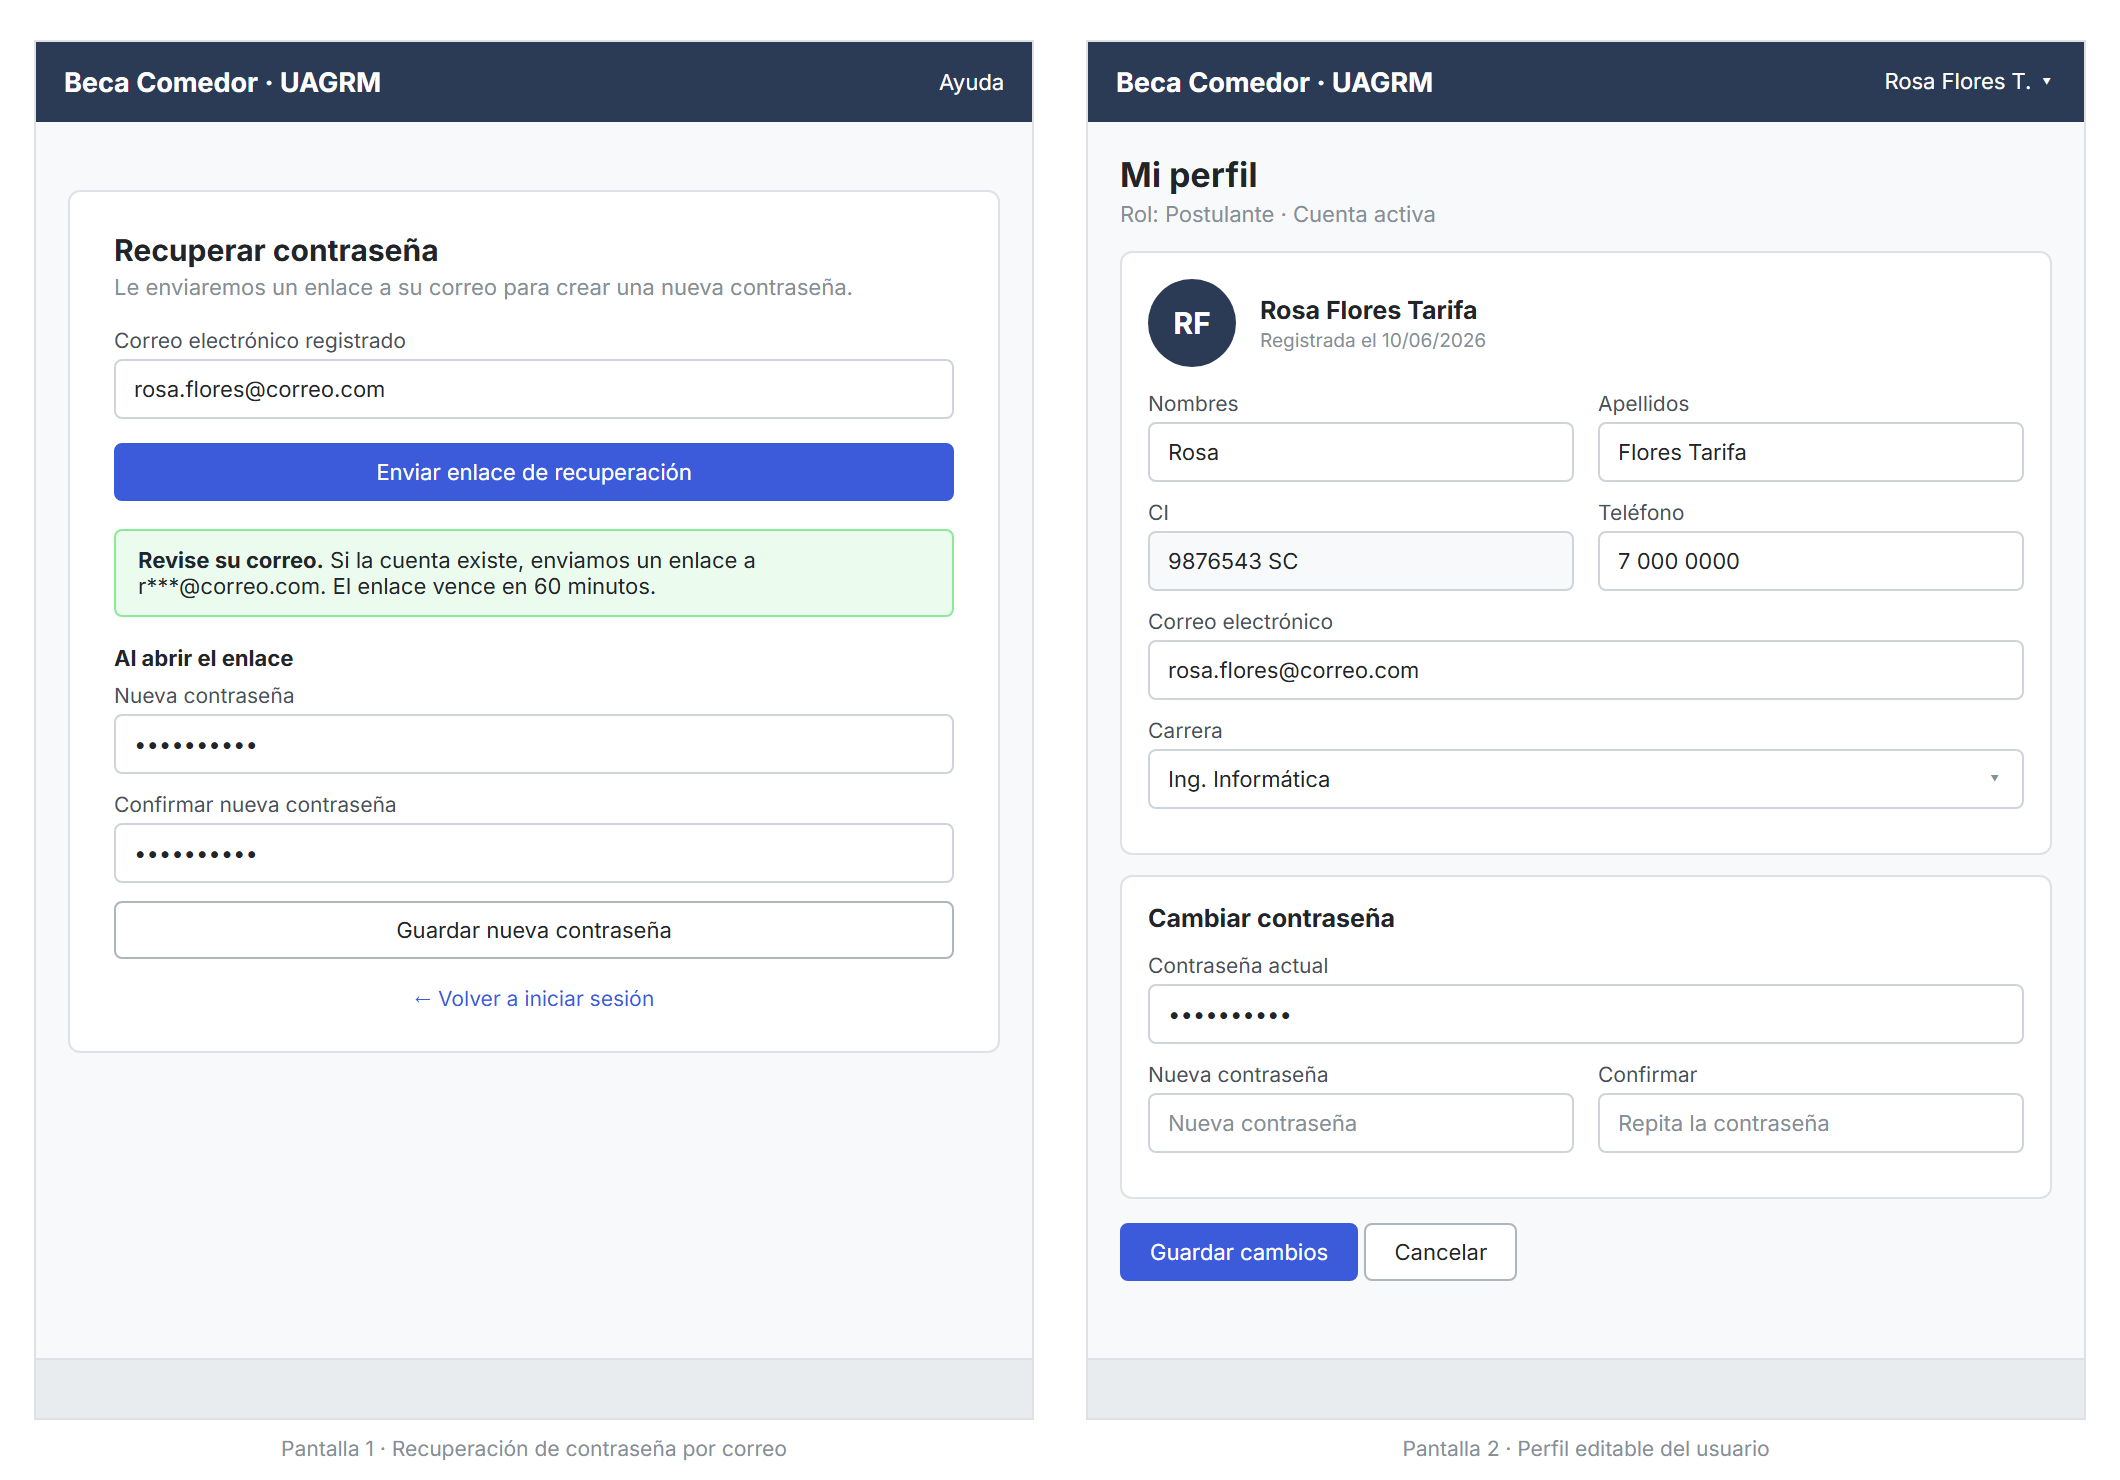
\includegraphics[width=\textwidth,height=0.75\textheight,keepaspectratio]{images/140_Mockup_CU15_Recuperar_contrasena_perfil.png}

\smallskip
\noindent\raggedright\textit{Nota.} Elaboración propia.
\end{figure}



\Needspace{0.9\textheight}
\wfb{\wn{7}.5.16. Interfaz CU-16 Digitalizar y adjuntar documentos}\label{sec:cap7_interfaz_cu16}

La Figura~\ref{fig:mockup_cu16} presenta la maqueta de interfaz del CU-16.

\begin{figure}[H]
\caption{Maqueta de interfaz del CU-16 Digitalizar y adjuntar documentos}
\label{fig:mockup_cu16}
\centering
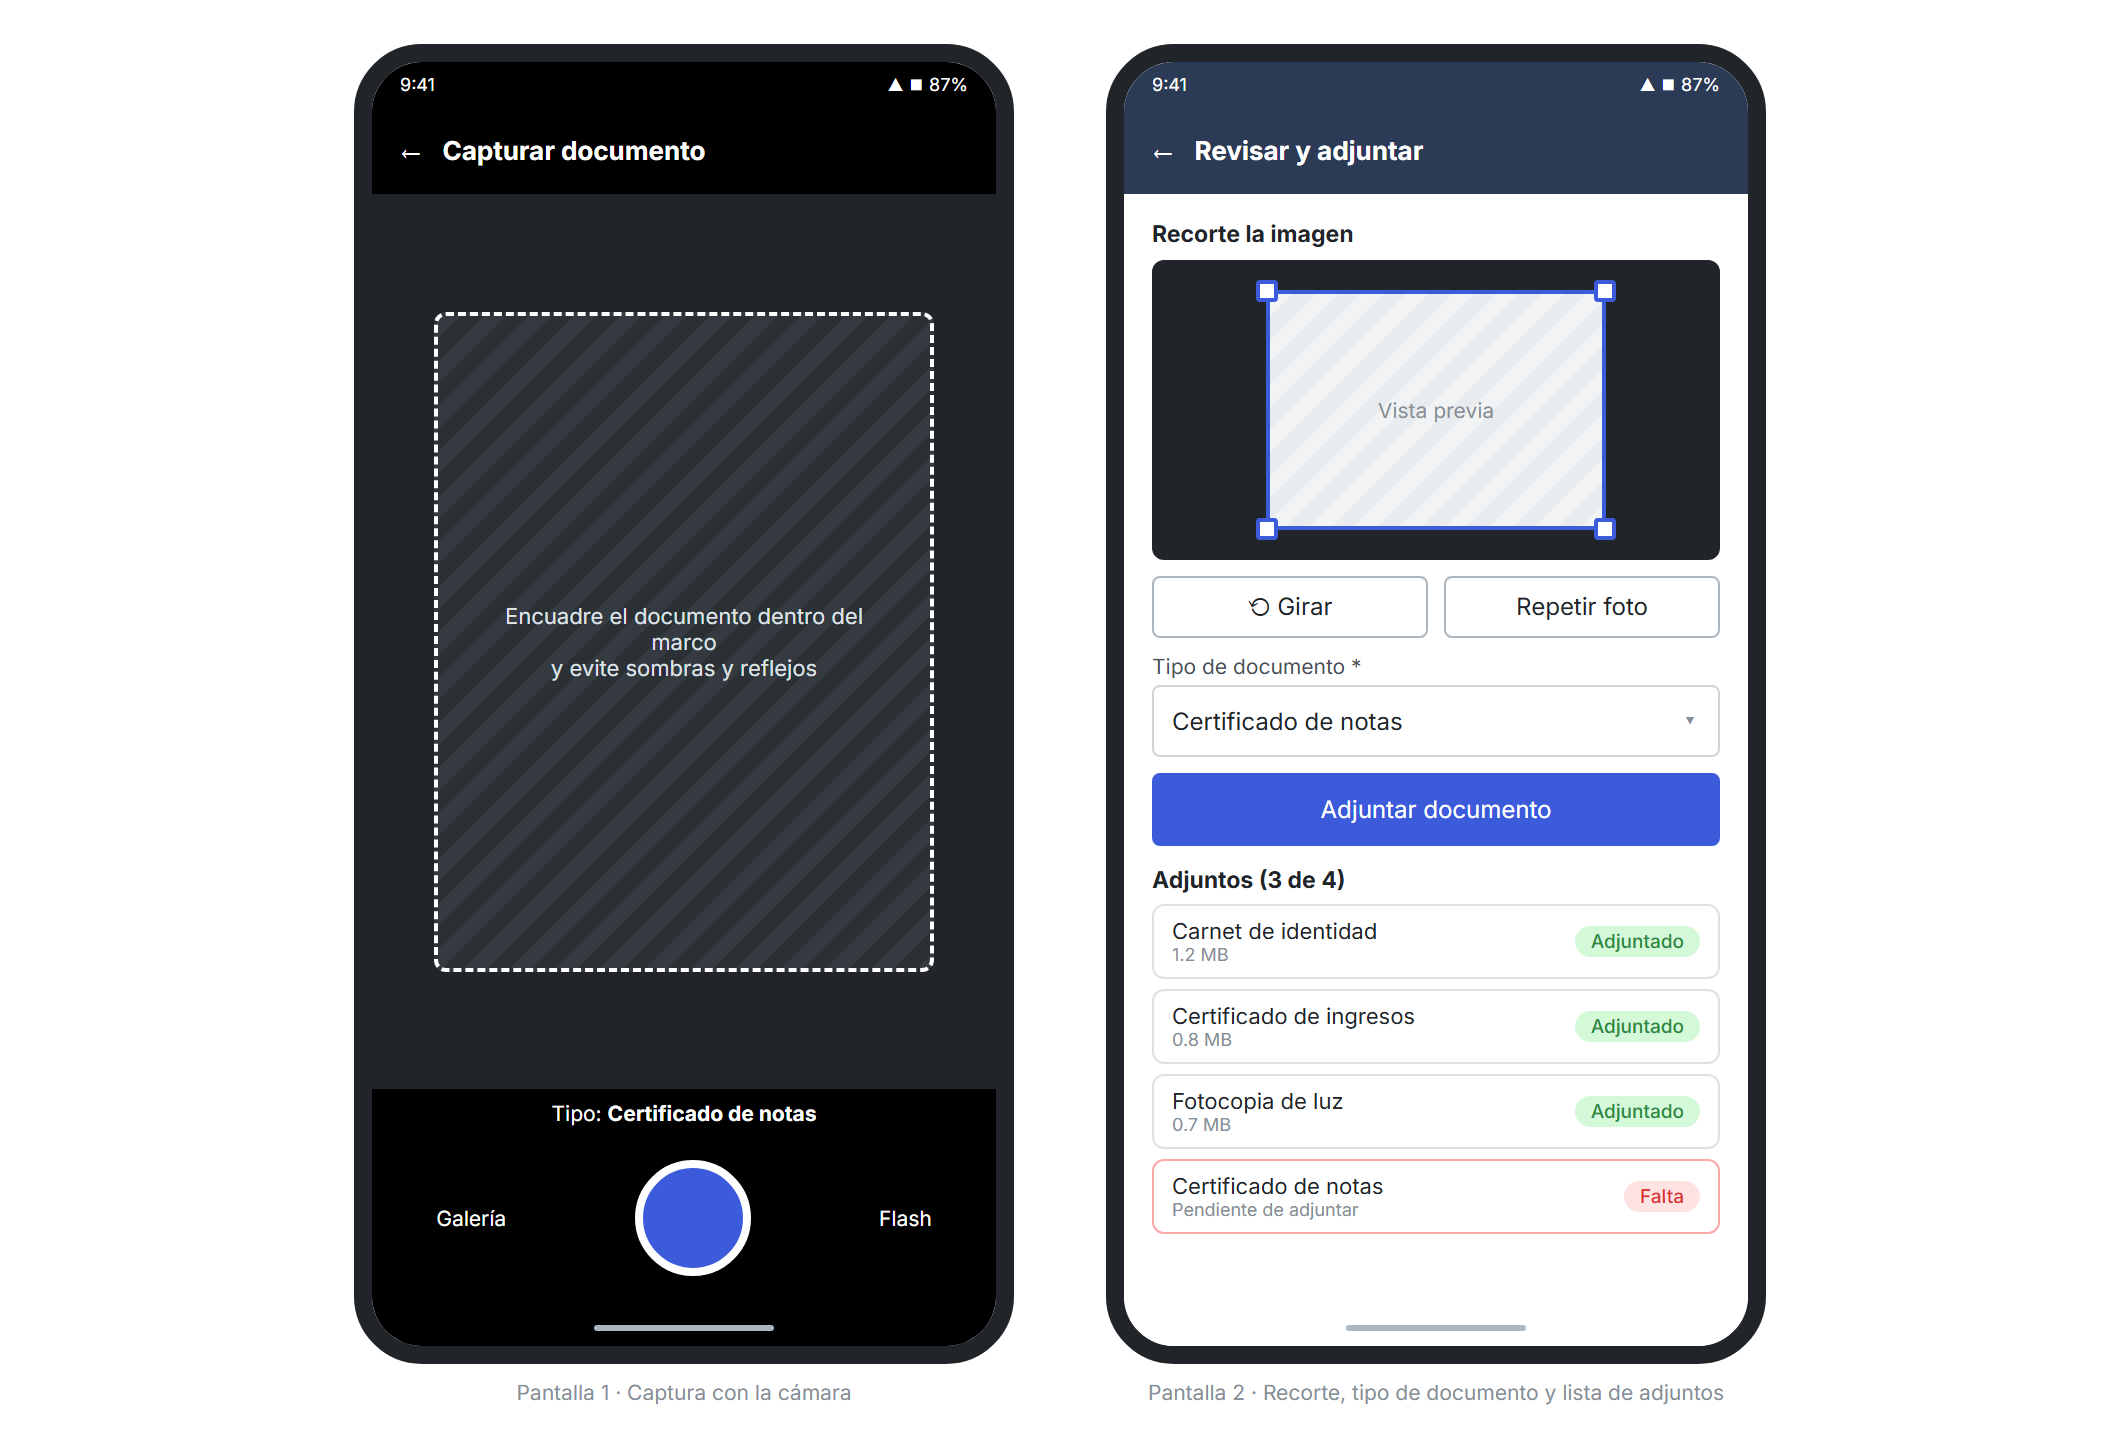
\includegraphics[width=\textwidth,height=0.75\textheight,keepaspectratio]{images/141_Mockup_CU16_Digitalizar_documentos.png}

\smallskip
\noindent\raggedright\textit{Nota.} Elaboración propia.
\end{figure}



\Needspace{0.9\textheight}
\wfb{\wn{7}.5.17. Interfaz CU-17 Guardar borrador de postulación}\label{sec:cap7_interfaz_cu17}

La Figura~\ref{fig:mockup_cu17} presenta la maqueta de interfaz del CU-17.

\begin{figure}[H]
\caption{Maqueta de interfaz del CU-17 Guardar borrador de postulación}
\label{fig:mockup_cu17}
\centering
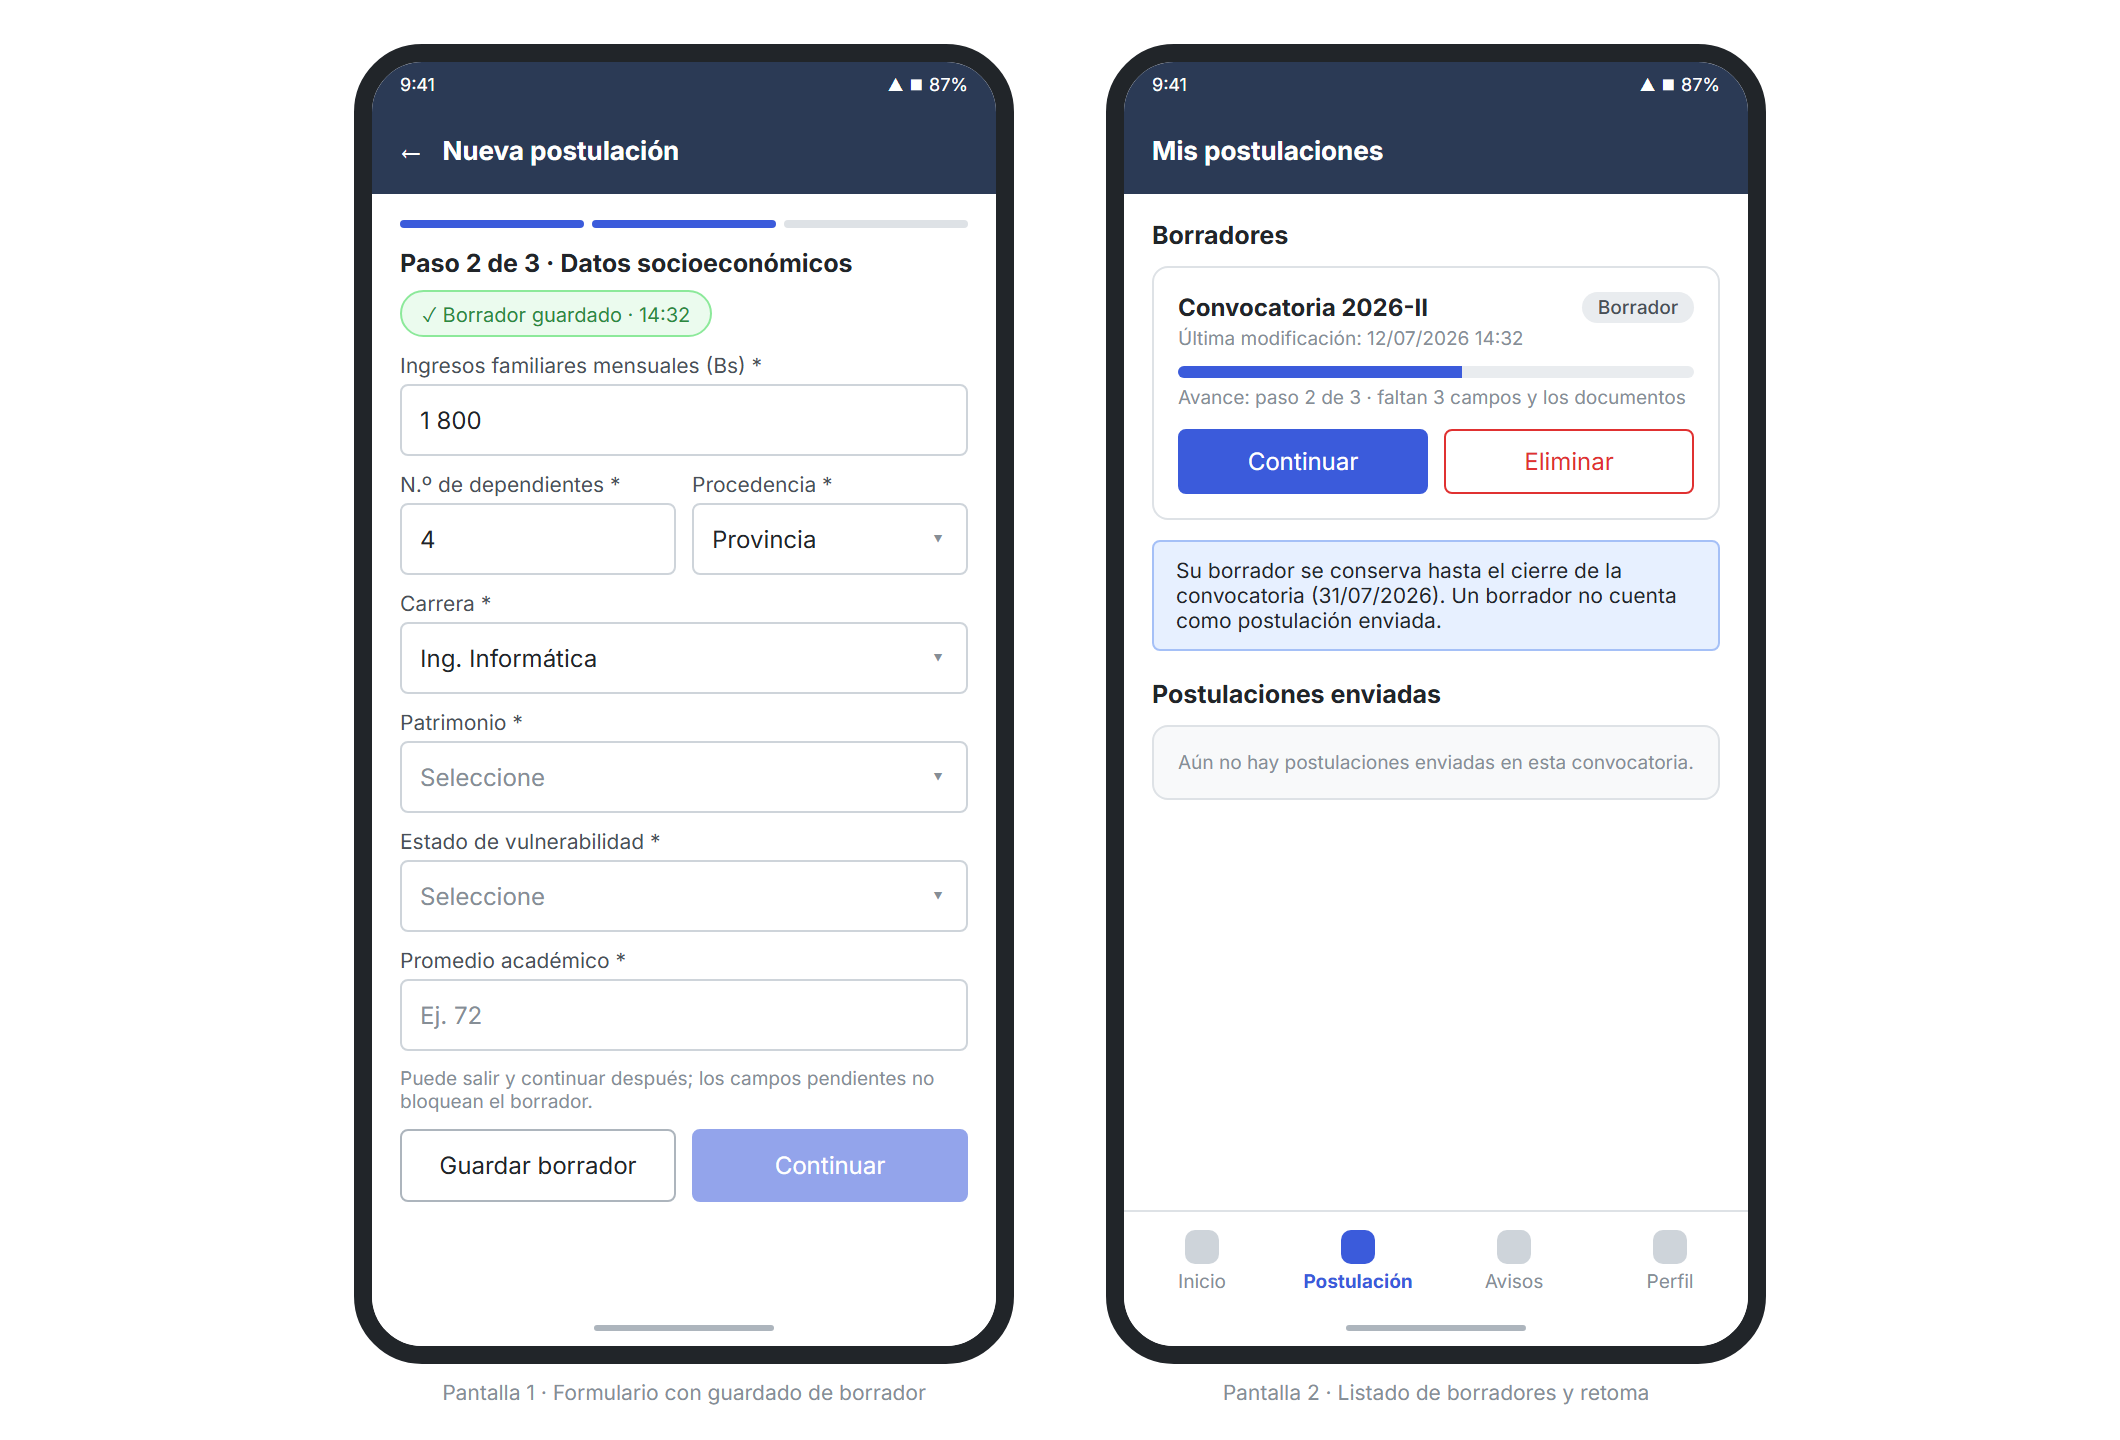
\includegraphics[width=\textwidth,height=0.75\textheight,keepaspectratio]{images/142_Mockup_CU17_Guardar_borrador.png}

\smallskip
\noindent\raggedright\textit{Nota.} Elaboración propia.
\end{figure}



\Needspace{0.9\textheight}
\wfb{\wn{7}.5.18. Interfaz CU-18 Validar elegibilidad y duplicados}\label{sec:cap7_interfaz_cu18}

La Figura~\ref{fig:mockup_cu18} presenta la maqueta de interfaz del CU-18.

\begin{figure}[H]
\caption{Maqueta de interfaz del CU-18 Validar elegibilidad y duplicados}
\label{fig:mockup_cu18}
\centering
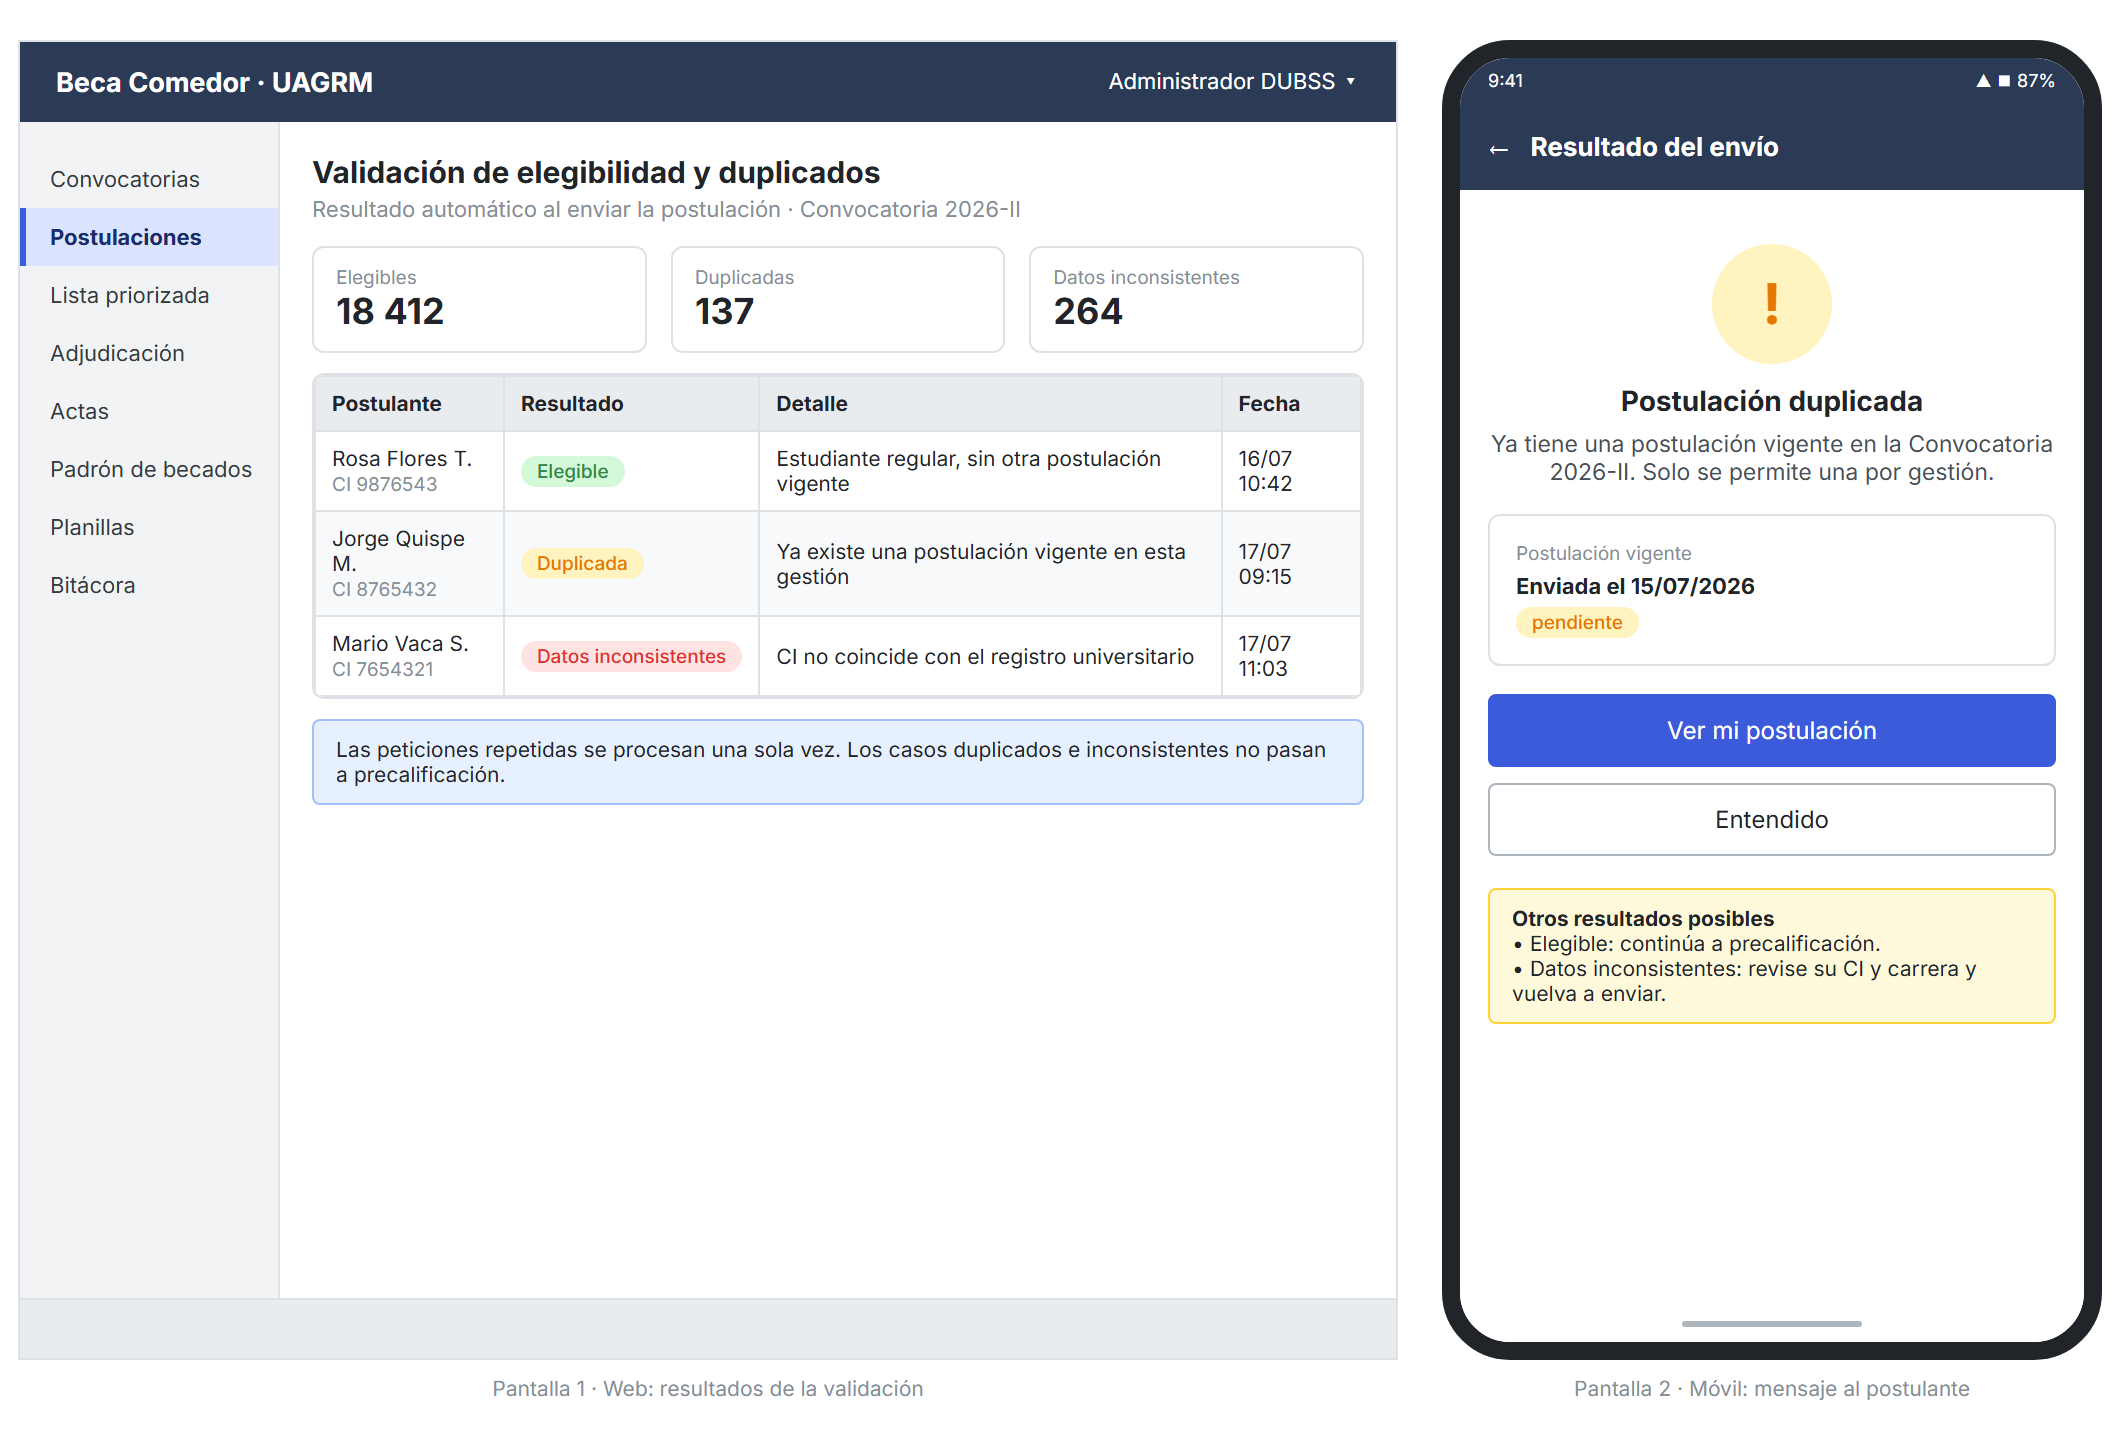
\includegraphics[width=\textwidth,height=0.75\textheight,keepaspectratio]{images/143_Mockup_CU18_Validar_elegibilidad.png}

\smallskip
\noindent\raggedright\textit{Nota.} Elaboración propia.
\end{figure}



\Needspace{0.9\textheight}
\wfb{\wn{7}.5.19. Interfaz CU-19 Devolver postulación para corrección}\label{sec:cap7_interfaz_cu19}

La Figura~\ref{fig:mockup_cu19} presenta la maqueta de interfaz del CU-19.

\begin{figure}[H]
\caption{Maqueta de interfaz del CU-19 Devolver postulación para corrección}
\label{fig:mockup_cu19}
\centering
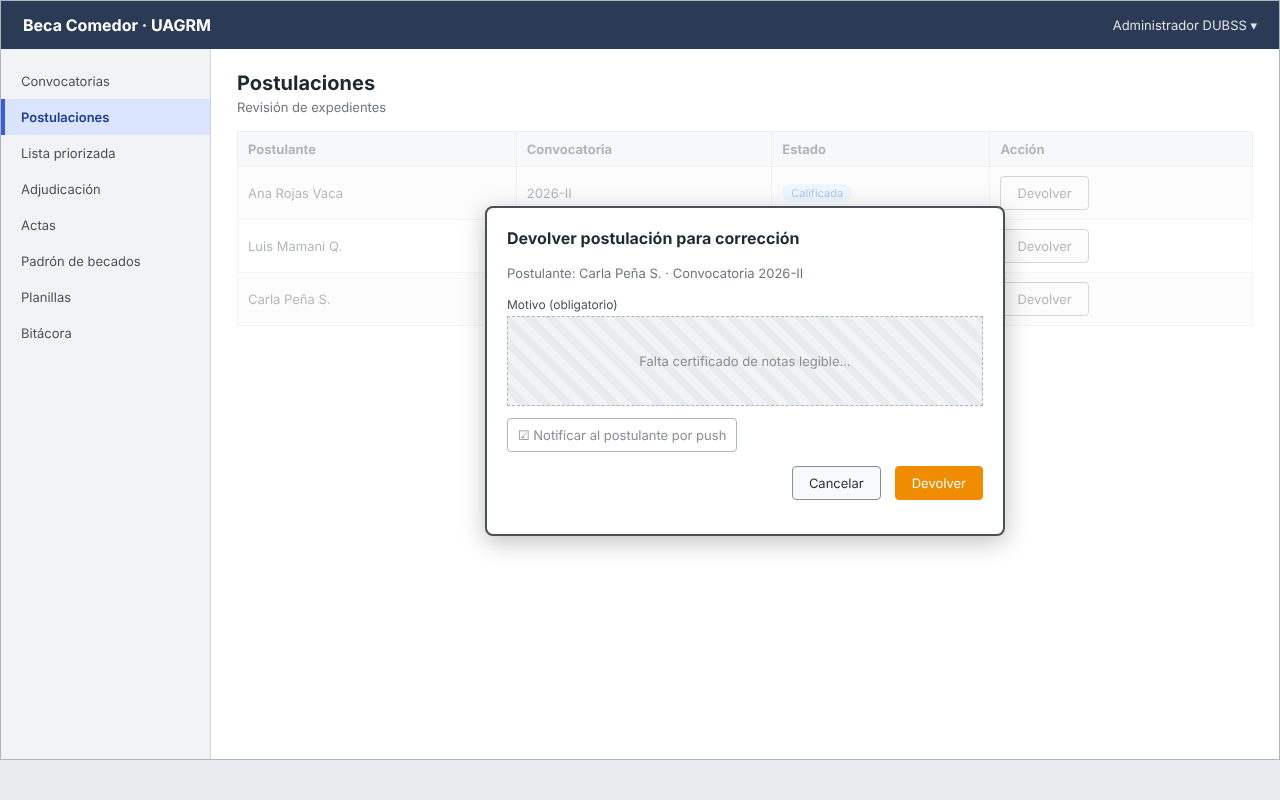
\includegraphics[width=\textwidth,height=0.75\textheight,keepaspectratio]{images/113_Mockup_CU19_Devolver_para_correccion.png}

\smallskip
\noindent\raggedright\textit{Nota.} Elaboración propia.
\end{figure}


\Needspace{0.9\textheight}
\wfb{\wn{7}.5.20. Interfaz CU-20 Archivar o rechazar postulación}\label{sec:cap7_interfaz_cu20}

La Figura~\ref{fig:mockup_cu20} presenta la maqueta de interfaz del CU-20.

\begin{figure}[H]
\caption{Maqueta de interfaz del CU-20 Archivar o rechazar postulación}
\label{fig:mockup_cu20}
\centering
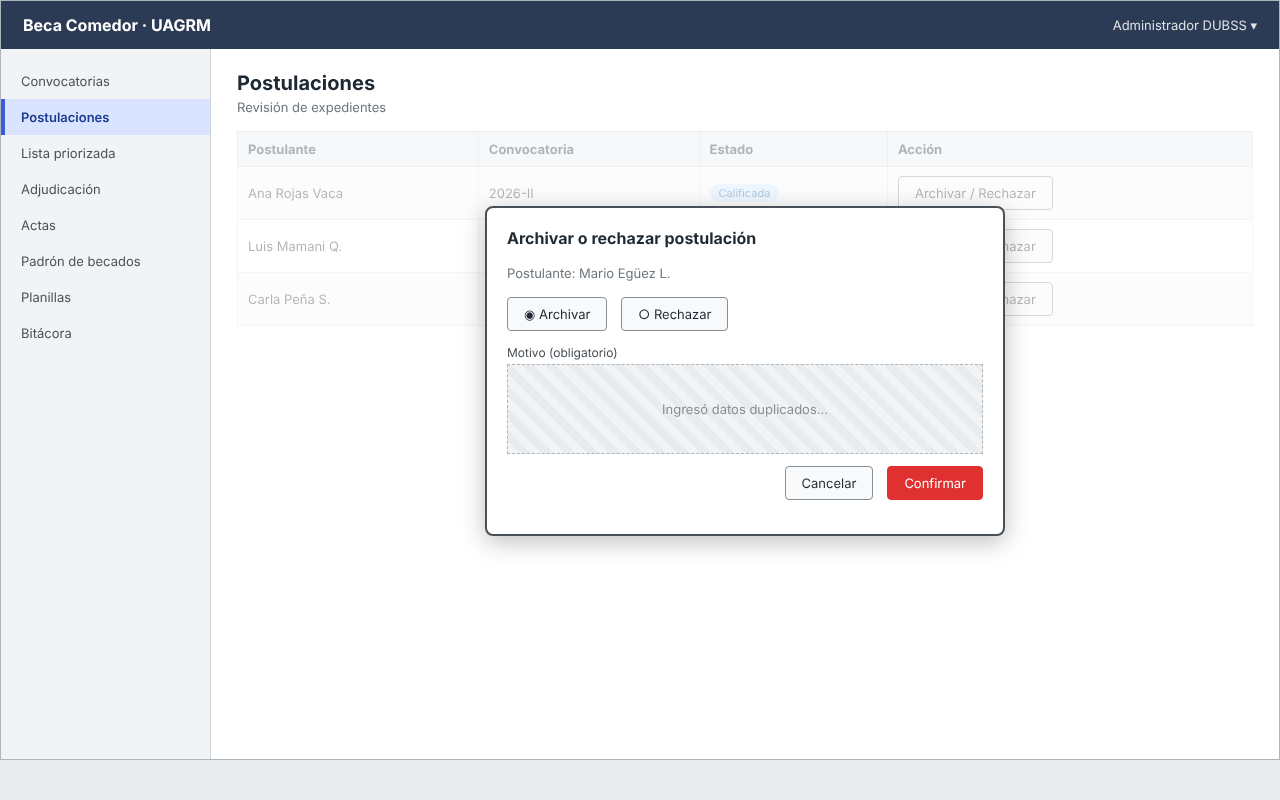
\includegraphics[width=\textwidth,height=0.75\textheight,keepaspectratio]{images/114_Mockup_CU20_Archivar_o_rechazar_postulacion.png}

\smallskip
\noindent\raggedright\textit{Nota.} Elaboración propia.
\end{figure}


\Needspace{0.9\textheight}
\wfb{\wn{7}.5.21. Interfaz CU-21 Notificar finalistas, registrar entrega de documentación física y publicar comunicados/avisos}\label{sec:cap7_interfaz_cu21}

La Figura~\ref{fig:mockup_cu21} presenta la maqueta de interfaz del CU-21.

\begin{figure}[H]
\caption{Maqueta de interfaz del CU-21 Notificar finalistas, registrar entrega de documentación física y publicar comunicados/avisos}
\label{fig:mockup_cu21}
\centering
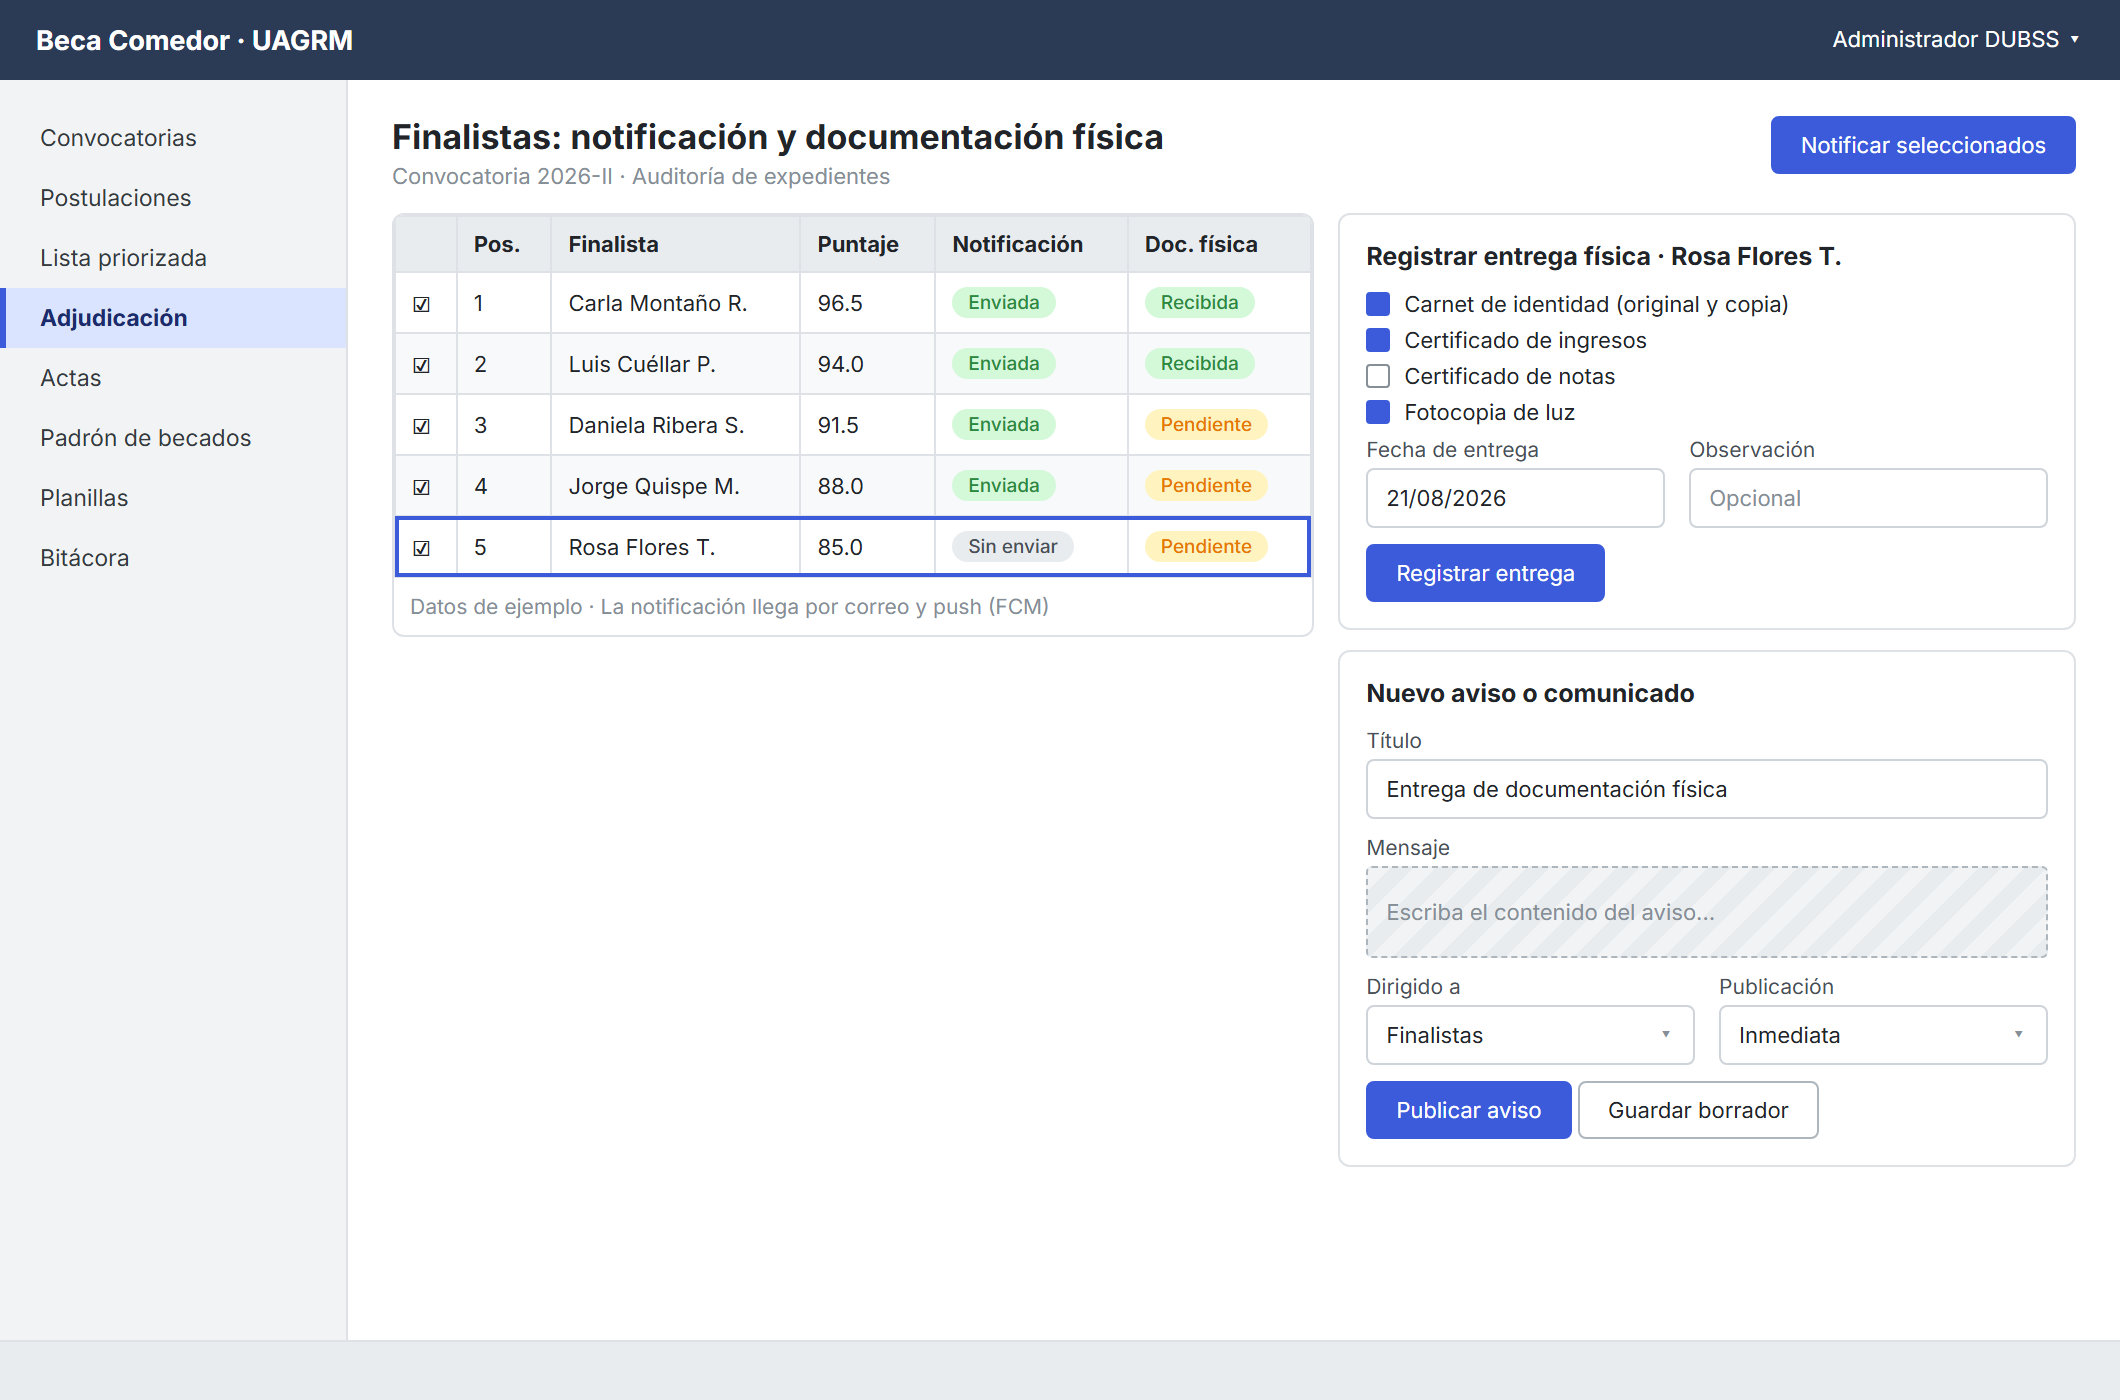
\includegraphics[width=\textwidth,height=0.75\textheight,keepaspectratio]{images/144_Mockup_CU21_Notificar_finalistas_avisos.png}

\smallskip
\noindent\raggedright\textit{Nota.} Elaboración propia.
\end{figure}



\Needspace{0.9\textheight}
\wfb{\wn{7}.5.22. Interfaz CU-22 Publicar resultados de adjudicación}\label{sec:cap7_interfaz_cu22}

La Figura~\ref{fig:mockup_cu22} presenta la maqueta de interfaz del CU-22.

\begin{figure}[H]
\caption{Maqueta de interfaz del CU-22 Publicar resultados de adjudicación}
\label{fig:mockup_cu22}
\centering
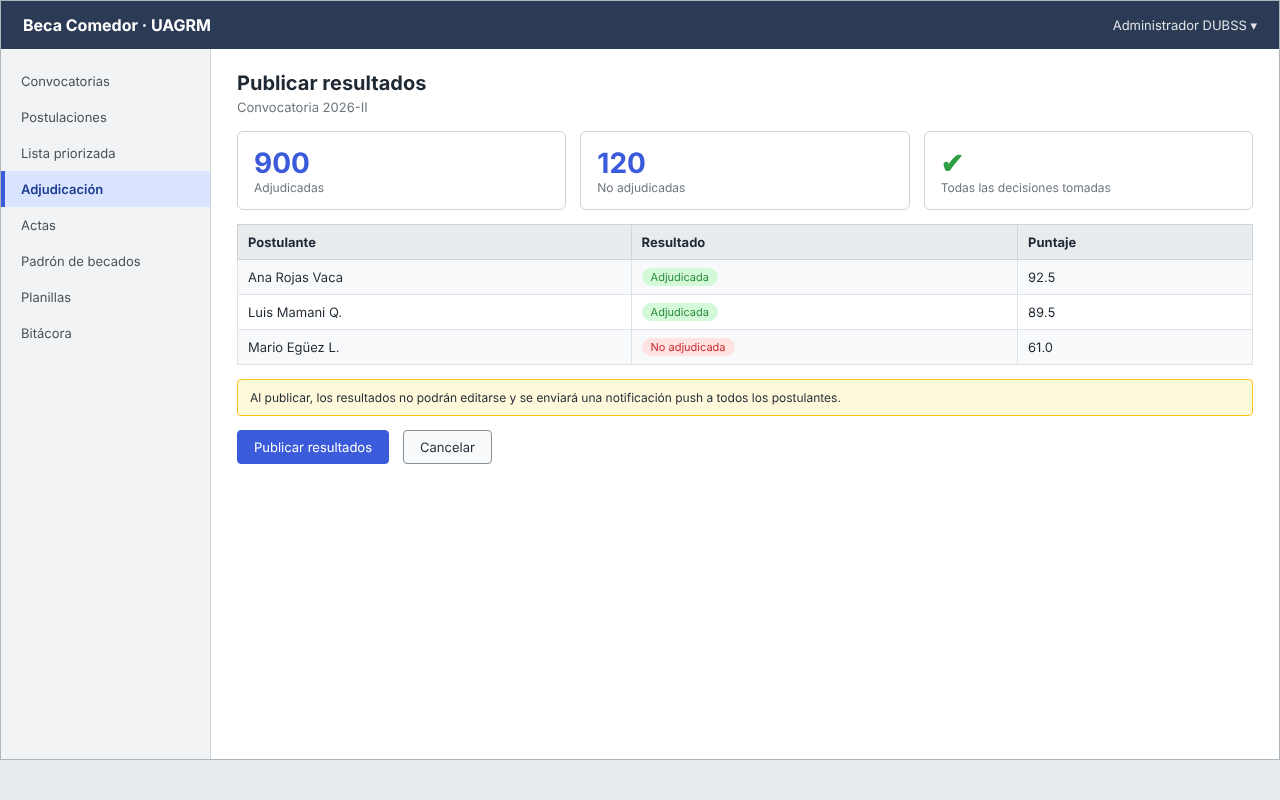
\includegraphics[width=\textwidth,height=0.75\textheight,keepaspectratio]{images/115_Mockup_CU22_Publicar_resultados.png}

\smallskip
\noindent\raggedright\textit{Nota.} Elaboración propia.
\end{figure}


\Needspace{0.9\textheight}
\wfb{\wn{7}.5.23. Interfaz CU-23 Gestionar padrón de becados (baja, suspensión, reemplazo)}\label{sec:cap7_interfaz_cu23}

La Figura~\ref{fig:mockup_cu23} presenta la maqueta de interfaz del CU-23.

\begin{figure}[H]
\caption{Maqueta de interfaz del CU-23 Gestionar padrón de becados (baja, suspensión, reemplazo)}
\label{fig:mockup_cu23}
\centering
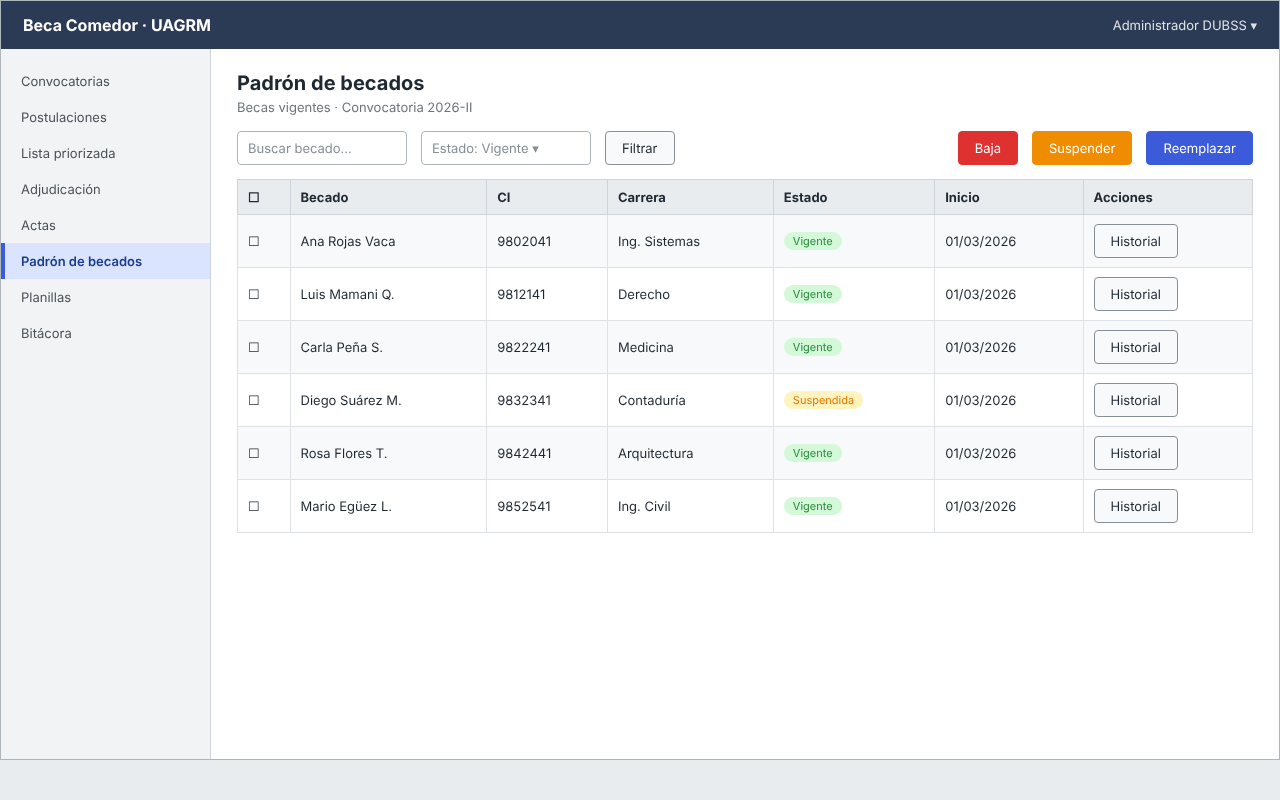
\includegraphics[width=\textwidth,height=0.75\textheight,keepaspectratio]{images/116_Mockup_CU23_Padron_de_becados.png}

\smallskip
\noindent\raggedright\textit{Nota.} Elaboración propia.
\end{figure}


\Needspace{0.9\textheight}
\wfb{\wn{7}.5.24. Interfaz CU-24 Consultar historial de asistencia y estado de beca}\label{sec:cap7_interfaz_cu24}

La Figura~\ref{fig:mockup_cu24} presenta la maqueta de interfaz del CU-24.

\begin{figure}[H]
\caption{Maqueta de interfaz del CU-24 Consultar historial de asistencia y estado de beca}
\label{fig:mockup_cu24}
\centering
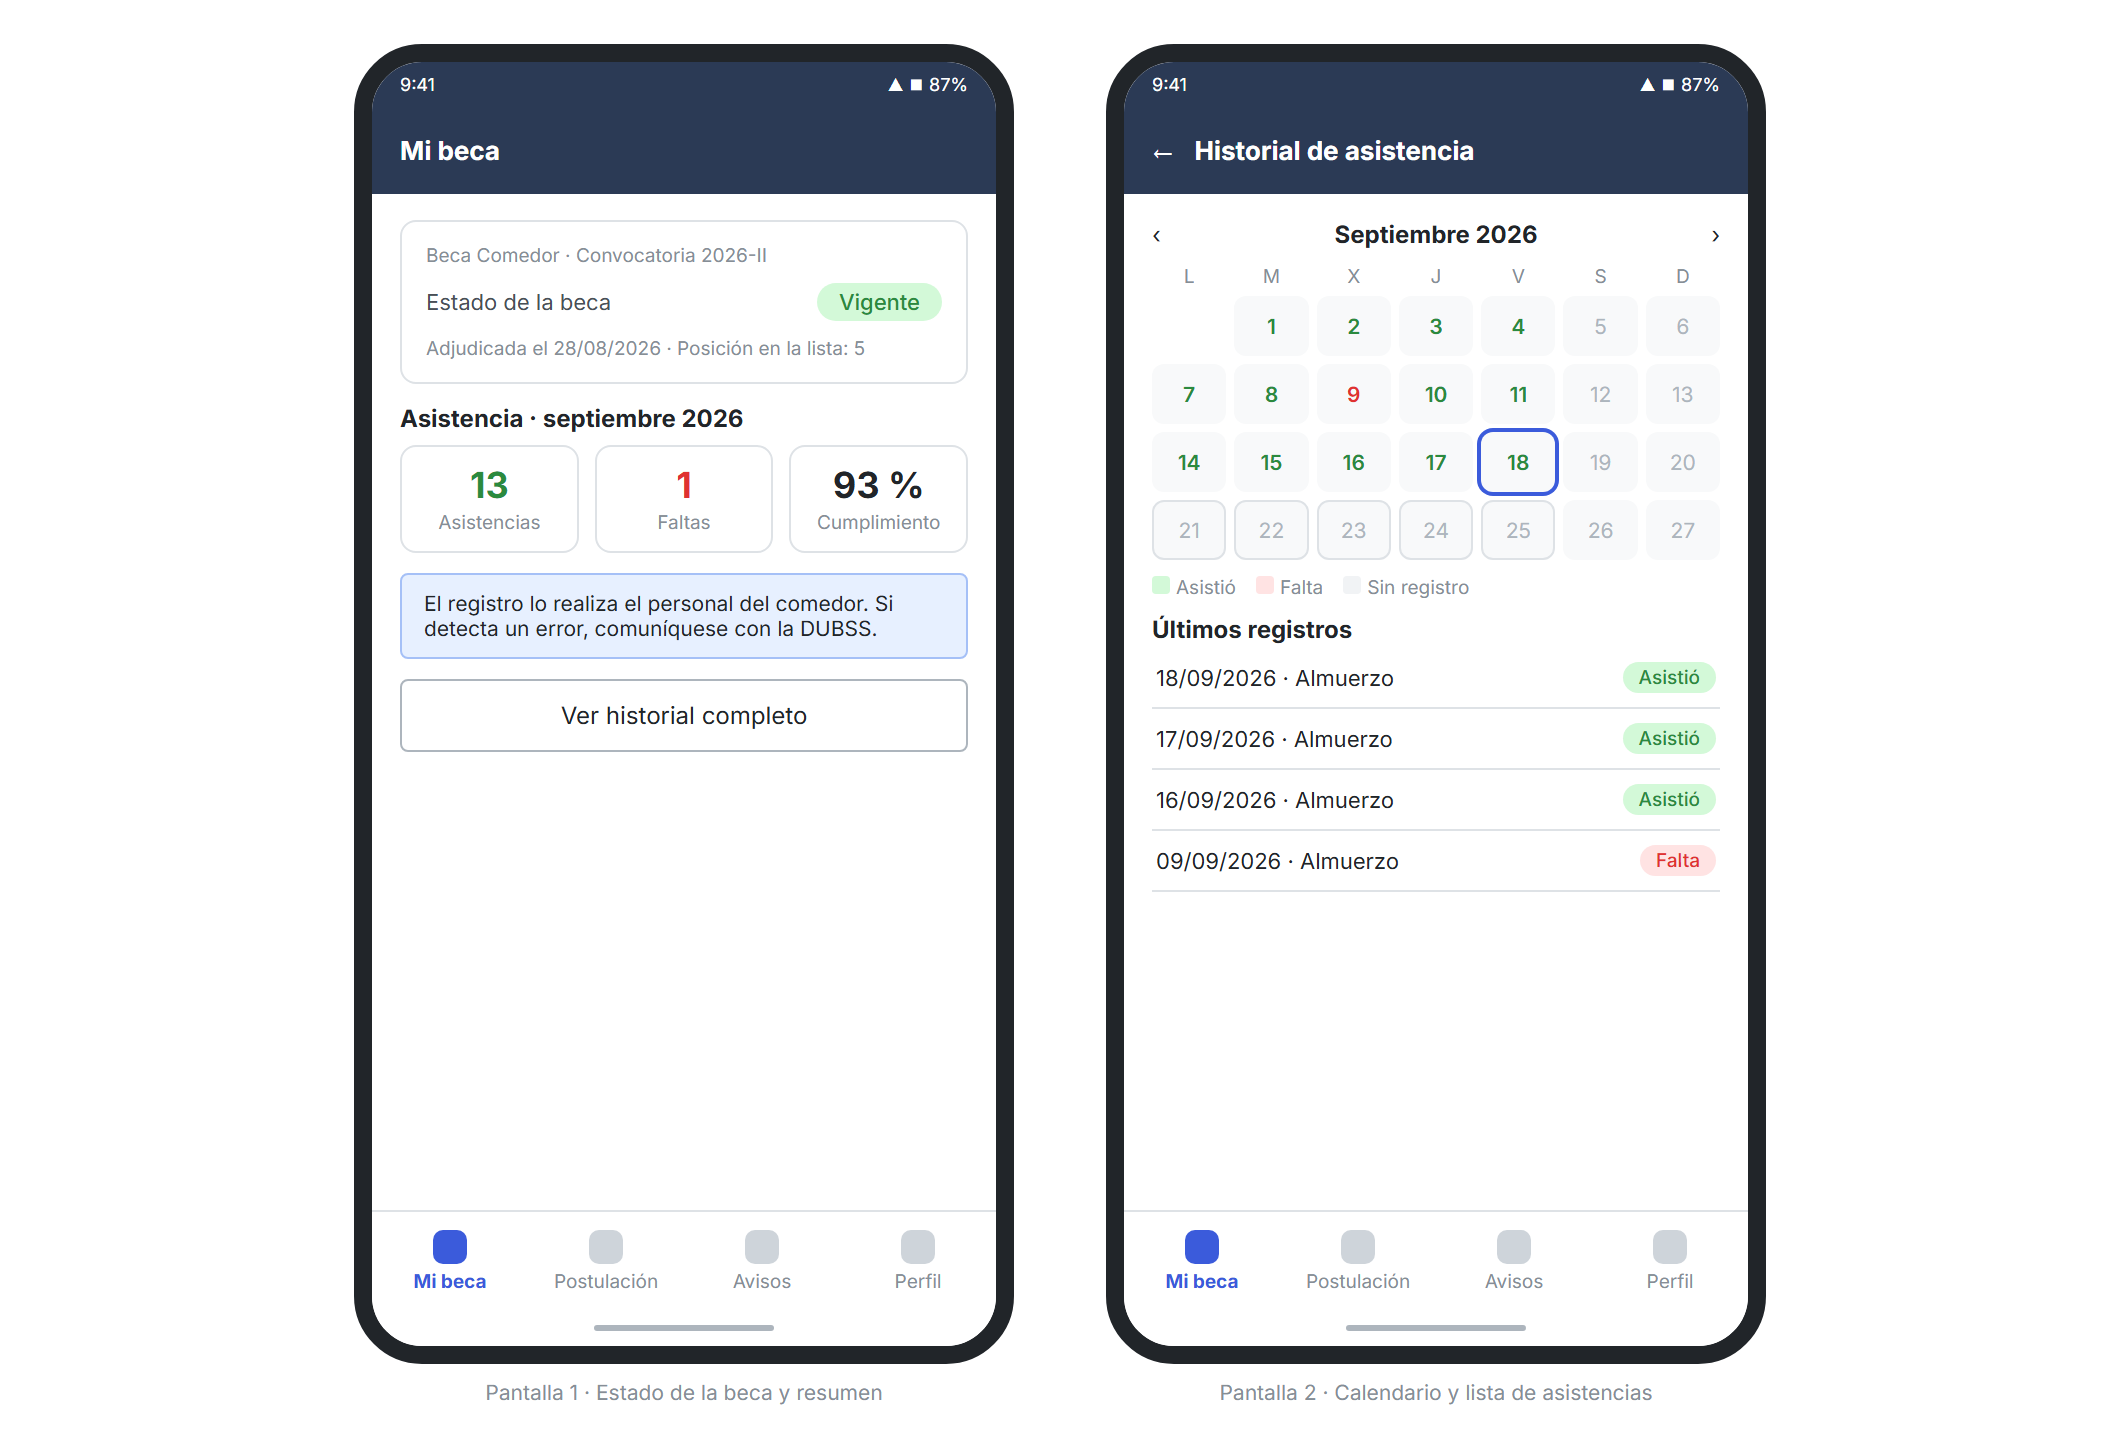
\includegraphics[width=\textwidth,height=0.75\textheight,keepaspectratio]{images/145_Mockup_CU24_Historial_asistencia.png}

\smallskip
\noindent\raggedright\textit{Nota.} Elaboración propia.
\end{figure}



\Needspace{0.9\textheight}
\wfb{\wn{7}.5.25. Interfaz CU-25 Consultar bitácora de acciones}\label{sec:cap7_interfaz_cu25}

La Figura~\ref{fig:mockup_cu25} presenta la maqueta de interfaz del CU-25.

\begin{figure}[H]
\caption{Maqueta de interfaz del CU-25 Consultar bitácora de acciones}
\label{fig:mockup_cu25}
\centering
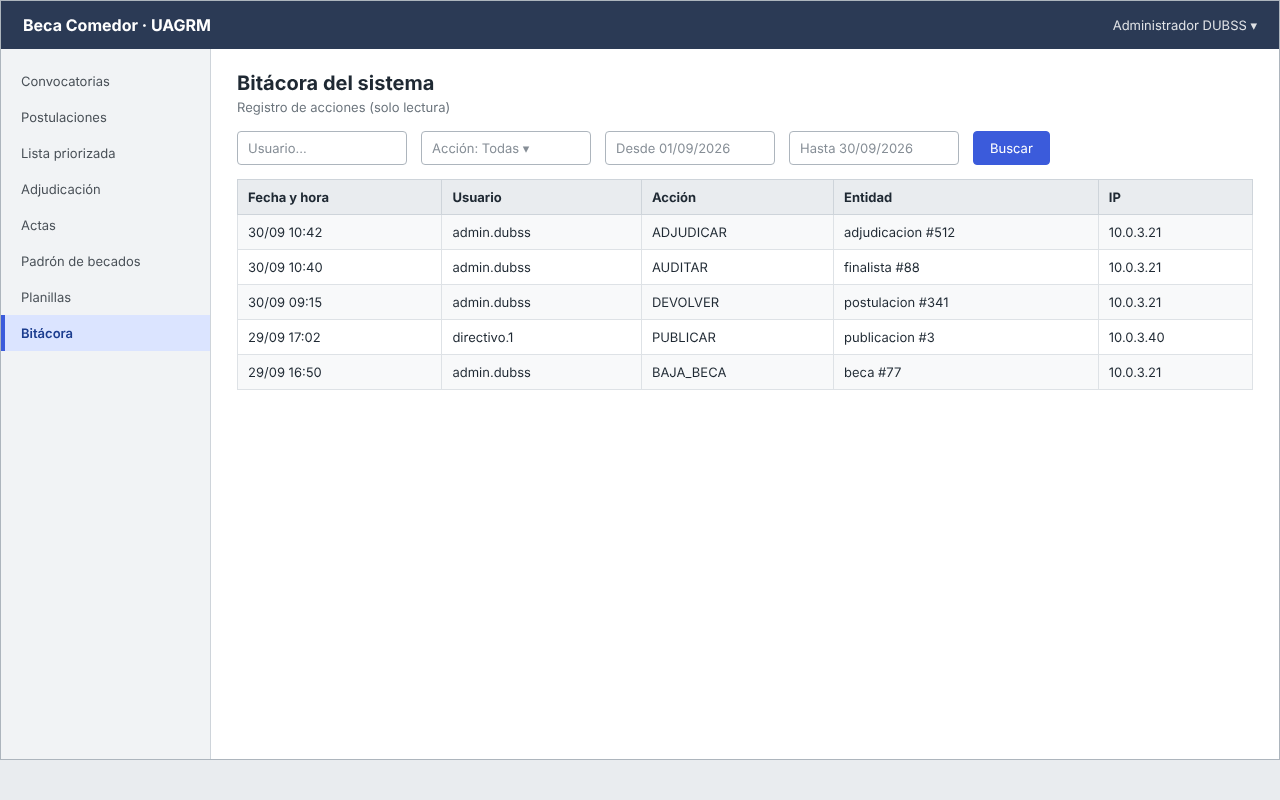
\includegraphics[width=\textwidth,height=0.75\textheight,keepaspectratio]{images/117_Mockup_CU25_Bitacora.png}

\smallskip
\noindent\raggedright\textit{Nota.} Elaboración propia.
\end{figure}


\Needspace{0.9\textheight}
\wfb{\wn{7}.5.26. Interfaz CU-26 Parametrizar modelo de preselección y reprocesar puntajes}\label{sec:cap7_interfaz_cu26}

La Figura~\ref{fig:mockup_cu26} presenta la maqueta de interfaz del CU-26.

\begin{figure}[H]
\caption{Maqueta de interfaz del CU-26 Parametrizar modelo de preselección y reprocesar puntajes}
\label{fig:mockup_cu26}
\centering
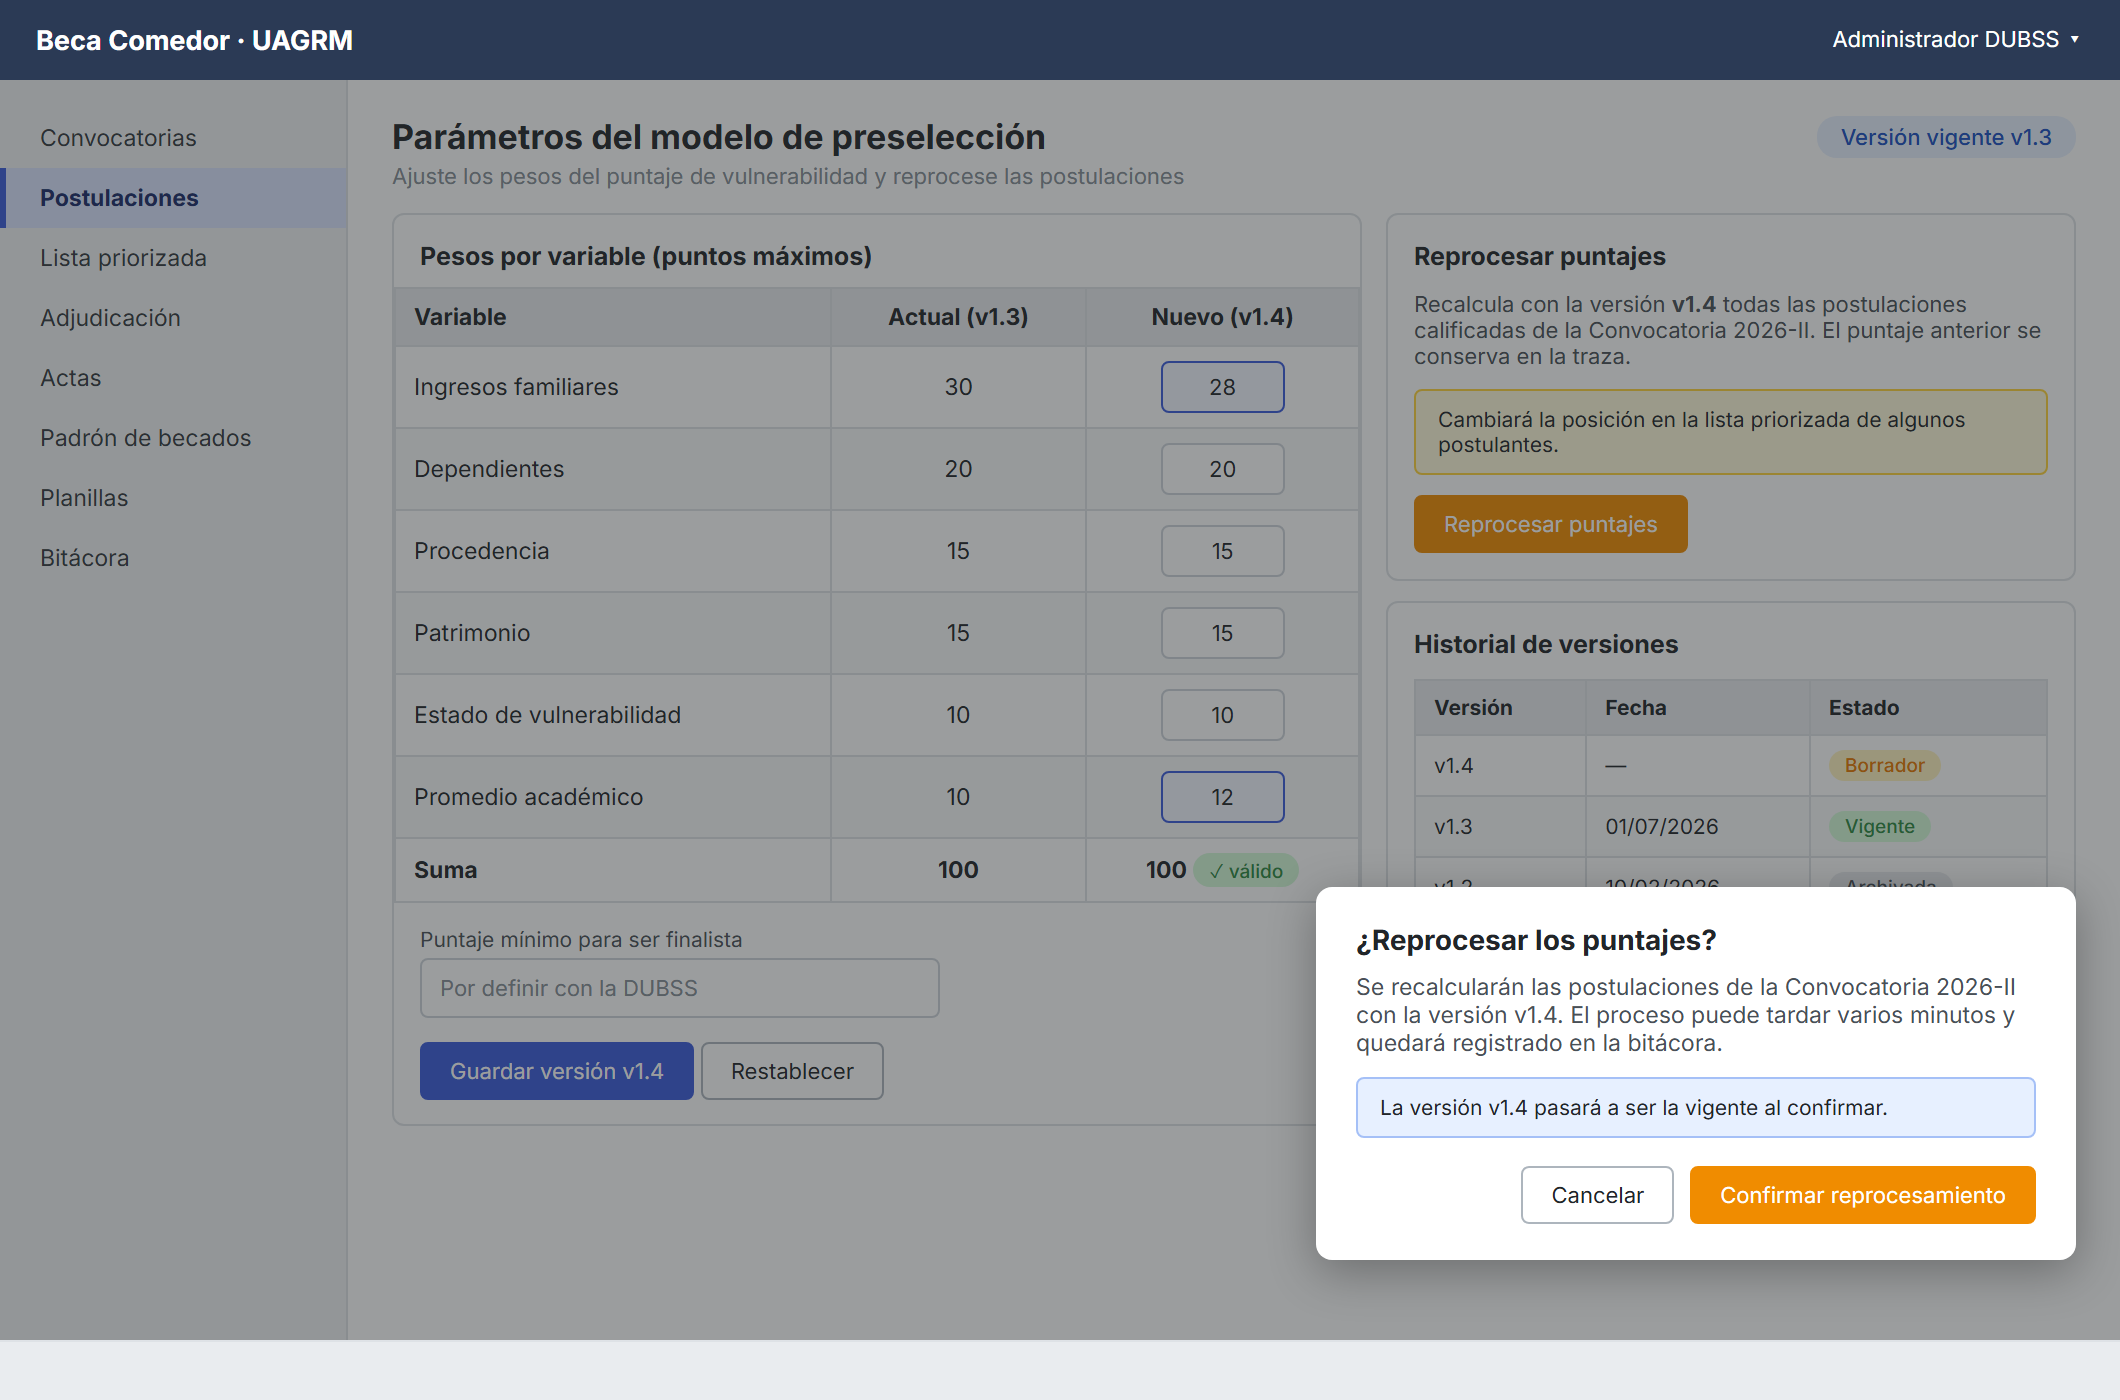
\includegraphics[width=\textwidth,height=0.75\textheight,keepaspectratio]{images/146_Mockup_CU26_Parametrizar_modelo.png}

\smallskip
\noindent\raggedright\textit{Nota.} Elaboración propia.
\end{figure}





% ==============================================================================
% 3.5 IMPLEMENTACIÓN (flujo de trabajo PUDS dentro del Capítulo 3)
% ==============================================================================
\subsection{3.5. Implementación}\label{cap:implementacion}

% [INSTRUCCIÓN]: Flujo de trabajo de Implementación del PUDS. Los seis paquetes corresponden a los paquetes identificados en la sección 3.3 (Análisis).

\subsubsection{3.5.1. Estrategia de Implementación}

% [PENDIENTE]: Redactar "Estrategia de Implementación".

\subsubsection{3.5.2. Estándares de Codificación}

Los estándares de codificación y de comentarios aplicados se definen en la sección 2.12 del Capítulo 2.

\subsubsection{3.5.3. Modelo de Implementación}

\paragraph{3.5.3.1. Diagrama de componentes}

% [PENDIENTE]: Redactar "Diagrama de componentes".

\paragraph{3.5.3.2. Diagrama de despliegue}

% [PENDIENTE]: Redactar "Diagrama de despliegue".

\subsubsection{3.5.4. Implementación por Paquetes}

\paragraph{3.5.4.1. Paquete Cuentas y Acceso}

% [PENDIENTE]: Redactar "Paquete Cuentas y Acceso".

\paragraph{3.5.4.2. Paquete Convocatoria y Postulación}

% [PENDIENTE]: Redactar "Paquete Convocatoria y Postulación".

\paragraph{3.5.4.3. Paquete Preselección con IA}

% [PENDIENTE]: Redactar "Paquete Preselección con IA".

\paragraph{3.5.4.4. Paquete Auditoría y Adjudicación}

% [PENDIENTE]: Redactar "Paquete Auditoría y Adjudicación".

\paragraph{3.5.4.5. Paquete Becados y Asistencia}

% [PENDIENTE]: Redactar "Paquete Becados y Asistencia".

\paragraph{3.5.4.6. Paquete Reportes y Trazabilidad}

% [PENDIENTE]: Redactar "Paquete Reportes y Trazabilidad".

\subsubsection{3.5.5. Integración y Construcción del Sistema}

% [PENDIENTE]: Redactar "Integración y Construcción del Sistema".

\subsubsection{3.5.6. Interfaces Implementadas}

\paragraph{3.5.6.1. Aplicación web}

% [PENDIENTE]: Redactar "Aplicación web".

\paragraph{3.5.6.2. Aplicación móvil}

% [PENDIENTE]: Redactar "Aplicación móvil".


% ==============================================================================
% 3.6 PRUEBAS (flujo de trabajo PUDS dentro del Capítulo 3)
% Las pruebas sobre el producto terminado y los mecanismos de prueba se desarrollan en el Capítulo 9.
% [PENDIENTE: CONFIRMAR] Los apartados 3.6.1 a 3.6.6 siguen las actividades del flujo de
% trabajo de Pruebas del Proceso Unificado; ajustarlos si el PUDS de la cátedra usa otros títulos.
% ==============================================================================
\subsection{3.6. Pruebas}\label{sec:v2_flujo_pruebas}

Este flujo de trabajo del PUDS verifica que el sistema implementado cumpla los requisitos especificados en la sección 3.2. Las pruebas sobre el producto terminado y los mecanismos de prueba utilizados se desarrollan en el Capítulo 9.

\subsubsection{3.6.1. Planificar las pruebas}

% [PENDIENTE]: Redactar "Planificar las pruebas".

\subsubsection{3.6.2. Diseñar las pruebas}

% [PENDIENTE]: Redactar "Diseñar las pruebas" (casos de prueba derivados de los casos de uso).

\subsubsection{3.6.3. Implementar las pruebas}

% [PENDIENTE]: Redactar "Implementar las pruebas".

\subsubsection{3.6.4. Realizar las pruebas de integración}

% [PENDIENTE]: Redactar "Realizar las pruebas de integración".

\subsubsection{3.6.5. Realizar las pruebas de sistema}

% [PENDIENTE]: Redactar "Realizar las pruebas de sistema".

\subsubsection{3.6.6. Evaluar las pruebas}

% [PENDIENTE]: Redactar "Evaluar las pruebas".


% ==============================================================================
% 3.7 a 3.9: ITERACIONES (PUDS)
% ==============================================================================
\subsection{3.7. Iteración 1}

\subsubsection{3.7.1. Planificación de la Iteración}

\paragraph{3.7.1.1. Casos de uso asignados.}

% [PENDIENTE]: Redactar "Casos de uso asignados".

\paragraph{3.7.1.2. Objetivo de la iteración.}

% [PENDIENTE]: Redactar "Objetivo de la iteración".

\paragraph{3.7.1.3. Proceso de desarrollo.}

\subparagraph{3.7.1.3.1. Diseño de la base de datos.}

% [PENDIENTE]: Redactar "Diseño de la base de datos".

\subparagraph{3.7.1.3.2. Diseño de la arquitectura.}

% [PENDIENTE]: Redactar "Diseño de la arquitectura".

\paragraph{3.7.1.4. Lista de tareas de la iteración.}

% [PENDIENTE]: Redactar "Lista de tareas de la iteración".

\subsubsection{3.7.2. Revisión de la Iteración}

% [PENDIENTE]: Redactar "Revisión de la Iteración".

\subsubsection{3.7.3. Retrospectiva de la Iteración}

% [PENDIENTE]: Redactar "Retrospectiva de la Iteración".

\subsection{3.8. Iteración 2}

\subsubsection{3.8.1. Planificación de la Iteración}

\paragraph{3.8.1.1. Casos de uso asignados.}

% [PENDIENTE]: Redactar "Casos de uso asignados".

\paragraph{3.8.1.2. Objetivo de la iteración.}

% [PENDIENTE]: Redactar "Objetivo de la iteración".

\paragraph{3.8.1.3. Proceso de desarrollo.}

\subparagraph{3.8.1.3.1. Diseño de la base de datos.}

% [PENDIENTE]: Redactar "Diseño de la base de datos".

\subparagraph{3.8.1.3.2. Diseño de la arquitectura.}

% [PENDIENTE]: Redactar "Diseño de la arquitectura".

\paragraph{3.8.1.4. Lista de tareas de la iteración.}

% [PENDIENTE]: Redactar "Lista de tareas de la iteración".

\subsubsection{3.8.2. Revisión de la Iteración}

% [PENDIENTE]: Redactar "Revisión de la Iteración".

\subsubsection{3.8.3. Retrospectiva de la Iteración}

% [PENDIENTE]: Redactar "Retrospectiva de la Iteración".

\subsection{3.9. Iteración 3}

\subsubsection{3.9.1. Planificación de la Iteración}

\paragraph{3.9.1.1. Casos de uso asignados.}

% [PENDIENTE]: Redactar "Casos de uso asignados".

\paragraph{3.9.1.2. Objetivo de la iteración.}

% [PENDIENTE]: Redactar "Objetivo de la iteración".

\paragraph{3.9.1.3. Proceso de desarrollo.}

\subparagraph{3.9.1.3.1. Diseño de la base de datos.}

% [PENDIENTE]: Redactar "Diseño de la base de datos".

\subparagraph{3.9.1.3.2. Diseño de la arquitectura.}

% [PENDIENTE]: Redactar "Diseño de la arquitectura".

\paragraph{3.9.1.4. Lista de tareas de la iteración.}

% [PENDIENTE]: Redactar "Lista de tareas de la iteración".

\subsubsection{3.9.2. Revisión de la Iteración}

% [PENDIENTE]: Redactar "Revisión de la Iteración".

\subsubsection{3.9.3. Retrospectiva de la Iteración}

% [PENDIENTE]: Redactar "Retrospectiva de la Iteración".

